\documentclass{article}
\usepackage[table]{xcolor}
\usepackage{tabularx} % for responsive width columns
\usepackage{array}
\usepackage{arxiv}

\usepackage{lipsum}
\usepackage{pgfgantt}
\usepackage[utf8]{inputenc} % allow utf-8 input
\usepackage[T1]{fontenc}    % use 8-bit T1 fonts
\usepackage{hyperref}       % hyperlinks
\usepackage{url}            % simple URL typesetting
\usepackage{booktabs}       % professional-quality tables
\usepackage{amsfonts}       % blackboard math symbols
\usepackage{nicefrac}       % compact symbols for 1/2, etc.
\usepackage{microtype}      % microtypography
\usepackage{graphicx}
\usepackage{pgf}
\usepackage{import}
\usepackage{longtable}
\usepackage[colorinlistoftodos]{todonotes}
\graphicspath{ {./images/} }

\usepackage[numbers,square]{natbib}
\usepackage{amsmath}
\usepackage{cleveref}
\usepackage{amssymb}
\usepackage{amsthm}
\usepackage{stmaryrd}
\usepackage{algorithmic,algorithm}
\usepackage{graphicx}
\usepackage{caption}
\usepackage{subcaption}
\usepackage{tikz}
\usetikzlibrary{positioning}
\usepackage{comment}


\Crefname{figure}{Figure}{Figures} % For capitalized (start of sentence)
\crefname{figure}{Figure}{Figures} % For lowercase
\Crefname{table}{Table}{Tables} % For capitalized (start of sentence)
\crefname{table}{Table}{Tables} % For lowercase

\definecolor{lightblue}{rgb}{0.93, 0.95, 1.0}
\definecolor{matplotlibblue}{rgb}{0.12, 0.47, 0.71}
\definecolor{lightyellow}{rgb}{1.0, 1.0, 0.6}
\definecolor{lightgreen}{rgb}{0.67, 0.88, 0.69}
\definecolor{weekend}{rgb}{0.83, 0.83, 0.83}
\definecolor{work}{rgb}{0.36, 0.54, 0.66}
% Define a new column type 'Y' that is like 'X' but with vertical centering
\newcolumntype{Y}{>{\centering\arraybackslash}X}

\newcommand{\cX}{\mathcal{X}}
\newcommand{\cL}{\mathcal{L}}
\newcommand{\cY}{\mathcal{Y}}

\newcommand{\bX}{\mathbf{X}}
\newcommand{\bY}{\mathbf{Y}}

% Caption spacing
% \setlength{\abovecaptionskip}{20pt} % Space above the caption
% \setlength{\belowcaptionskip}{20pt} % Space below the scaption


\newtheorem{definition}{Definition}
\newtheorem{remark}{Remark}
\newtheorem{proposition}{Proposition}
\newtheorem{corollary}{Corollary}

% \title{The First Line of my Research Proposal Title\\is Followed by the Optional Second Line of the\\Research Proposal Title}
\title{Topic Modeling of OpenML Dataset Descriptions}


\author{
 Ivan, Germanov \\
 ID: 1483838 \\
 Artificial Intelligence and Data Engineering Lab\\
Eindhoven University of Technology\\
  \texttt{i.germanov@student.tue.nl} \\
}

\begin{document}
\maketitle
\begin{abstract}
    {
        \color{red}
        Provide an informative summary of your proposal (topic, approach and potential importance of the results) in no more than three hundred words.
        %
        Make sure to provide an informative and relevant abstract, as this is often the first part of your proposal that reviewers will read. The abstract should clearly describe what you are going to investigate, why you are going to investigate this subject and which results you expect to find.
        %
        The abstract should have no more than 300 words and should contain a single paragraph.
        %
        This proposal should be self-contained and has a limit of pages per section. \textbf{Title page, Abstract, Sections 1 and 2 have a combined limit of 8 pages. Section 3 has a limit of 8 pages. Section 4 has a limit of 2 pages. References and Appendices are unlimited.} You should not change the overall format considerably. Please do not change the margins nor introduce considerable LaTeX code that try to compress the content. You may use the appendices for any further information that you want to provide. While there is no page limit in the appendix, reviewers are not obliged to read all your appendix content.

        \noindent\textbf{Wordcount: 190}
    }
\end{abstract}

%%------------------------------------------------------------------------------
\section{Overall aim and goals}
\label{sec:goals}
%%------------------------------------------------------------------------------
\subsection{Motivation and Challenges}
% {
% \color{red}
% This section provides a motivation for the project, which may come from a business case, a scientific interest from the research community, or any other motivation. It is useful to explain the problem here and contextualise it, explain the (scientific) relevance and challenges, as well as the originality and innovative character. In some cases, it might be preferable to reorder the subsections within the same Section~\ref{sec:goals}. This is a valid change to the template.
% }

Topic modeling is a rapidly growing field with applications in various contexts that include text corpora - social media posts \cite{curiskis_evaluation_2020,paul_discovering_2014,pennacchiotti_investigating_2011}, books \cite{raj_p_m_sentiment_2022}, newspapers \cite{jacobi_quantitative_2018,nicholson_search_2020,marjanen_topic_2020}, legal documents \cite{silveira_topic_nodate,oneill_analysis_2016}, research papers \cite{asmussen_smart_2019} and financial reports \cite{el_mokhtari_using_2020,garcia-mendez_automatic_2023}, to name a few. Topic models can take a large corpus of documents as input and extract the latent topics present therein \cite{blei_latent_2001}. A topic refers to a recurring pattern of words or phrases that commonly occur together in a set of documents \cite{abdelrazek_topic_2022}.

\citet{churchill_evolution_2022} define a topic model to be a mathematical model that takes as input a set of documents $D$, and returns a set of topics $T$ that represent the content of $D$ in an accurate and coherent manner. The documents within the collection can subsequently be tagged with these identified topics. This process enables users to discern the importance of each topic both within individual documents and across the entire collection.

OpenML \cite{vanschoren_openml_2014} is a platform designed for machine learning researchers to share and manage data. It facilitates global collaboration by allowing users to present new datasets for analysis and share their findings, including code, models, predictions, and evaluations. OpenML ensures the clear definition of tasks and organizes all contributions online for easy accessibility, reuse, and discussion.

For each dataset, OpenML provides a dedicated page that contains detailed information such as a general dataset description, attribution details, and characteristics of the data, as well as statistics on the data distribution. Additionally, OpenML supports the use of tags on datasets, facilitating easier filtering and searchability.

\subsubsection{Motivation}
In OpenML, datasets are currently categorized using manual tagging. However, many datasets lack semantic tags that are readable by humans. This situation presents an opportunity for a Master's thesis project aimed at developing an automated system for tagging datasets. Given that most datasets come with descriptions, applying topic modeling to extract topics can be an innovative approach to generate and assign relevant tags.

Applying topic modeling to extract topics as tags could enhance how users interact with the OpenML platform. Specifically, it could make the process of searching and filtering through the extensive collection of datasets more efficient, thus enhancing dataset discoverability. The addition of semantic tags based on the topics identified in the descriptions could also lead to better organization and management of datasets, thereby improving data governance on the platform.

Automating the process of tagging can save considerable time for researchers and data scientists who would otherwise have to tag datasets manually. This method ensures consistency in the tags applied and enriches the datasets' metadata, making them more useful and accessible.

Furthermore, previous work by \citeauthor{das_openmlscripts_nodate} has shown the potential of using scripts to automate the tagging of datasets in OpenML \cite{das_openmlscripts_nodate}. \citeauthor{das_openmlscripts_nodate}'s approach involved using dataset descriptions and a predefined list of tags to prompt GPT-3.5-turbo to assign relevant semantic tags to each dataset. This method demonstrated the feasibility of classifying datasets with a set of predefined tags, similar to the dataset tags in the Wolfram Data Repository \cite{noauthor_wolfram_nodate}.

This research aims to explore the potential of topic modeling when applied to dataset descriptions, an area that to our knowledge has not been extensively studied. By doing so, it seeks to contribute new insights to the field of topic modeling, which has been applied in various contexts but not extensively in the categorization of datasets based on their descriptions.

\subsubsection{Challenges}
One challenge encountered is the absence of comprehensive descriptions for datasets on OpenML. A significant number of these datasets lack descriptions or possess only short ones. Furthermore, the available descriptions often present difficulties in topic extraction due to their semi-structured nature, incorporating elements such as author names, dates, and attribute information. To address this issue, it may be necessary to . To address this issue, it may be necessary to identify additional datasets with adequate descriptions for training the topic model, while excluding datasets with inadequate descriptions from topic extraction and tagging process.

The absence of ground truth values for evaluating the performance of the proposed topic model presents another challenge. A ground truth value, such as "Economics" for a dataset containing longitudinal S\&P 500 price data, is an example of what is missing from the OpenML datasets. Consequently, identifying and selecting appropriate evaluation metrics to measure the extracted topics and tags' quality is necessary.

% \todo[inline]{

% - Speak about business case in OpenML (\citet{vanschoren_openml_2014}) - semantic tagging.

% - Talk about application of ChatGPT to classify topics by Taniya - this demonstrates potential of project.

% - Speak about originality and innovative character - nobody has applied topic modeling on dataset descriptions.

% Taniya:
% for Motivation we can also include 
% 1. Organising large corpus of datasets, enhancing discoverability. we can now provide users with a more comprehensive set of keywords and topics associated with each dataset. so improved search. 
% 2. Automated topic/tag generation would be uniform across datasets. 
% 3. enriches already present metadata information.

% Challenges:
% Need to mention challenges. Some could be:
% 1. dataset description can be ambiguous/ lack enough details sometimes. 
% 2. finding an appropriate training data for topic model. Available datasets might not be sufficient. 
% 3. In our use case, we do not have ground truth values (directly, but can be found in some cases using the original repo url), so need to find good evaluation measures.
% etc.
% }


%%------------------------------------------------------------------------------
\subsection{Broad Literature Analysis}\label{sec:broadliterature}
% {
% \color{red}
% This part presents some background for the project, including a broad literature analysis that puts the proposal in context. It describes previous work in general terms, but typically does not go deep into the technical details, which are instead later presented in the Background (Section~\ref{sec:background}). This can include, for instance, a complete literature analysis and description of the approaches that could be compared, such as baselines and competitors, to the research proposed here. These citations in the end of this sentence make no sense with the rest of the text here but are given as example of how to cite other papers~\citep{al2019predicting,alotaibi2020applications}.

% This is an example of an equation:
% \begin{eqnarray}
%     \label{eq:example}
%     \cX + \cY & \leq & \left[ \cL \cdot (\bX \times \bY) \right]\\
%     a + b & = & c + d \nonumber
% \end{eqnarray}
% \noindent
% and it is possible to make a comment about Expression~\eqref{eq:example} in the text. Typically equations are seldom present in a broad literature analysis and often appear in a more in-depth background section. Yet, there are exceptions to this rule, in particular when those technical details are needed to build the case for the proposal and to describe the formulation of the problem and objectives clearly.
% }

\subsubsection{Early Foundations and Probabilistic Models}
The origins of topic models can be traced back to the early 1990s with the development of Latent Semantic Indexing (LSI), introduced by \citet{deerwester_indexing_1990}. LSI creates a word-document matrix from a given vocabulary and a collection of documents. This matrix records how frequently each word in the vocabulary appears in the documents. The key step in LSI is the use of singular value decomposition (SVD). SVD compresses the dimensionality of documents, while still maintaining the meaning of the words.

LSI served as a precursor to topic models. In 1999, \citet{hofmann_probabilistic_1999} introduced Probabilistic Latent Semantic Indexing (pLSI). In pLSI, the SVD component of LSI was replaced with a generative data model known as an \textit{aspect model}. This change enabled the training of the model using an expectation maximization algorithm. Instead of deriving topics through SVD, \citeauthor{hofmann_probabilistic_1999}'s approach allowed topics to emerge as probabilistic mixtures of words. These mixtures were based on the joint probabilities of words and documents. This probabilistic framework marked a departure from the earlier matrix factorization approach of LSI and laid the groundwork for more advanced topic modeling techniques.

In 2000, \citet{nigam_text_2000} explored how to integrate unlabeled data into text classification, leading to the development of the Dirichlet Multinomial Mixture (DMM). They employed expectation maximization in conjunction with the Dirichlet distribution \cite{de_theorie_1814}. The Dirichlet distribution is a multivariate extension of the Beta distribution. Unlike the Beta distribution, which is defined by parameters $\alpha$ and $\beta$, the Dirichlet distribution is characterized by a parameter $k$. This $k$ represents the number of dimensions in the Dirichlet distribution. These dimensions collectively form a normalized probability distribution, which is adjusted using the parameter $\alpha$. The Dirichlet distribution is particularly suitable for topic modeling, as each topic can be represented as one of the $k$ dimensions in the distribution.

\subsubsection{Latent Dirichlet Allocation}
The term "topic model" was coined by \citet{blei_latent_2001} in their seminal 2001 paper on Latent Dirichlet Allocation (LDA). This work adopted the use of a generative model in a similar way to pLSI, but bases its model on the Dirichlet distribution. LDA introduced the concept that documents can be associated with multiple topics, rather than a single topic, as was the case with previous models. Furthermore, a key advancement of LDA was its capacity to be applied to new, unseen documents. The influence of LDA in topic modeling has been substantial, leading to numerous works improving upon LDA, and on the creation of LDA variants adapted for various tasks \cite{jelodar_latent_2019, teh_sharing_2004, lafferty_correlated_2005, blei_dynamic_2006, chemudugunta_modeling_2006, nallapati_multiscale_2007, wang_continuous_2012, iwata_topic_2009, banerjee_topic_2007, porteous_fast_2008, yao_efficient_2009, hoffman_online_2010}.

Most topic models, including LDA, are unsupervised. However, for some tasks, supervision is required. To address this, a variant of LDA named Supervised Latent Dirichlet Allocation (sLDA) was developed, which transforms LDA into a supervised model \citet{mcauliffe_supervised_2007}. sLDA extends LDA by associating a response variable with each document. The aim of sLDA is to discover latent topics that are both descriptive of the documents and predictive of the response variable. It achieves this by using a generalized linear model to connect the response variable with the topic proportions in each document.

The evolution of topic models has been influenced by changes in the types of data being analyzed, as noted by \citet{churchill_evolution_2022}. In the 2000s, the primary data sources for topic models were scientific articles, books, and newspapers. However, the landscape has shifted in recent years, with an increasing focus on digital and social media content such as tweets, blog posts, and Reddit posts.

Despite the change in data types, LDA and its variants have remained prevalent in the field. These models have been recognized as best practices for various data types and continue to be relevant. However, the field of topic modeling has progressed to include newer models beyond LDA.

\subsubsection{Non-negative Matrix Factorization and Other Topic Models}
Non-negative Matrix Factorization (NMF) represents one of the newer advancements in topic modeling, as highlighted by \citet{churchill_evolution_2022}. NMF is a technique where an original matrix, consisting of non-negative values, is decomposed into two distinct matrices. The fundamental principle of NMF is that the product of these two matrices approximates the original matrix. This decomposition is a form of dimensionality reduction. The large original matrix typically represents a set of documents, with each document being a vector of words. The two resultant matrices in NMF are the topic-word matrix and the topic-document matrix. The topic-word matrix shows the association between topics and words, while the topic-document matrix shows the relationship between topics and individual documents.

The application of NMF in topic modeling was first demonstrated by \citet{shahnaz_document_2006}. They showcased the potential of NMF as a tool for extracting topics from a collection of documents. Following this, \cite{kasiviswanathan_emerging_2011} expanded the application of NMF to temporal topic models. \citet{yan_learning_2013} later augmented NMF by replacing the document-term matrix with a term correlation matrix to detect topics in short texts.

In their 2013 study, \citet{yan_biterm_2013} presented the Biterm Topic Model (BTM). This model is specifically tailored for analyzing short texts, like tweets and social media updates. Instead of focusing on patterns within entire documents, BTM works by identifying and analyzing pairs of words, termed 'biterms'. These biterms are formed based on a distribution of topics and words.

In 2015, \citet{quan_short_2015} introduced the Self-Aggregating Topic Model (SATM), aimed at improving the topic modeling of short texts. SATM comprises two steps. Initially, it runs LDA on short texts. Subsequently, it uses the topics generated in the first step to create longer pseudo-texts. A pseudo-text in this context refers to the concatenation of shorter documents into a single, longer document.

In 2014, \citet{yin_dirichlet_2014} augmented the Dirichlet Multinomial Mixture (DMM) by introducing the Gibbs Sampling DMM. This adaptation incorporated the Gibbs sampling algorithm, specifically aimed at more effective modeling of short texts. This innovative approach to the established DMM model paved the way for further advanced variations of DMM.

Following this advancement, \citet{li_topic_2016} proposed two models: the Generalized Polya Urn Dirichlet Multinomial Mixture (GPUDMM) and the Generalized Polya Urn Poisson-based Dirichlet Multinomial Mixture (GPUPDMM). These models, similar to the approach by \citet{nguyen_improving_2015}, integrate word embeddings into the classic DMM model. In the GPU approach, when a word is selected, a copy of that word along with similar words are added back to the topic. This mechanism leads to clusters of similar words rising to the forefront of a topic, thus creating topics with more coherent and related sets of words. Regarding the DMM aspect of their models, \citeauthor{li_topic_2016} directly draw from \cite{yin_dirichlet_2014}'s GSDMM \citeauthor{yin_dirichlet_2014}.

Building upon DMM, \citet{li_filtering_2018} developed the Common Semantics Topic Model (CSTM). In this model, they introduced a concept known as 'common topics', designed to capture words that are prevalent across all topics. CSTM then creates topics by combining words from a single specific topic with words from these common topics.

\subsubsection{Graph-based Topic Models}
Graph-based models are another approach to topic modeling that followed LDA. In these models, words are represented as nodes in a graph, with their co-occurrences indicated by weighted edges. This method diverges from previous generative models by not assuming any underlying topic distribution, which facilitates the discovery of topics of varying sizes.

\citet{cataldi_emerging_2010} were among the first to implement a graph-based model using a directed graph to detect emerging topics. Subsequently, \citet{de_arruda_topic_2016} developed a topic model known as Topic Segmentation (TS), which was based on an undirected graph. In 2018, the Topic Flow Model (TFM) was introduced by \citet{churchill_temporal_2018}, applying graph-based methods to track the evolution of topics over time. Following this, \citet{churchill_percolation-based_2020} proposed the Percolation-based Topic Model (PTM), a graph-based model designed to detect topics within noisy datasets.

\subsubsection{Word Embedding Topic Models}
The integration of natural language processing (NLP) techniques into topic models marks a recent advancement in the field, diverging from earlier statistical models like LDA. A key development in this area has been the use of pre-trained NLP models to augment the capabilities of unsupervised topic models.

According to \citet{almeida_word_2023}, the most prominent form of NLP models employed in this context is word embedding spaces. The inception of word embeddings can be traced back to the early 2000s with the work of \citet{bengio_neural_2000}, who proposed a neural model for learning distributed representations of words.

A seminal study in the field of NLP for creating word embeddings is Word2Vec by \citet{mikolov_efficient_2013}. This study demonstrated the efficacy of word vectors in identifying semantically similar words. Word2Vec itself comprises two distinct architectures that facilitate the learning of high-quality word embeddings: Skip-gram and Continuous Bag of Words (CBOW).

\citet{nguyen_improving_2015} later enhanced the LDA and DMM models by incorporating word embeddings, resulting in two new models: Latent Feature LDA (LF-LDA) and Latent Feature DMM (LF-DMM). In these models, they added a word embedding component to the topic-word distribution of LDA and DMM. LF-LDA and LF-DMM maintain the original structure of LDA and DMM, but integrate a word embedding for each word in their distributions. When generating words for a document, the model can select words either from the topic's distribution or from the word embedding associated with that topic. This approach effectively enlarges the selection pool of words. The addition of the word embedding component improves the models' performance, especially when dealing with short texts.

\citet{qiang_topic_2017} developed the Embedding-based Topic Model (ETM), which leverages Word2Vec and introduces a new distance metric known as Word Mover's Distance (WMD). WMD calculates the minimum cumulative distance that words in one document need to travel to match the closest corresponding words in another document. After computing WMD, ETM combines short documents into longer pseudo-texts. Subsequently, LDA is applied to these pseudo-texts to determine topic assignments. The model then constructs an undirected graph to create a Markov Random Field. In this framework, similar words appearing in the same pseudo-text are more likely to be assigned to the same topic.

\citet{bunk_welda_2018} proposed another enhancement to LDA, termed Word Embedding LDA (WELDA). This approach involves integrating a pretrained word embedding model with a slightly modified version of LDA.

\citet{li_dirichlet_2019} further adapted the Dirichlet Multinomial Mixture (DMM) model to better suit short texts, creating the Laplacian DMM (LapDMM). This model integrates variational manifold regularization to maintain the local neighborhood structure inherent in short texts. Before training LapDMM, a graph is constructed to measure the distances between documents, identifying their nearest neighbors. This graph's Laplacian matrix is then utilized as a constraint in the topic assignment process. This ensures that documents assigned to the same topic contain words that are located in similar neighborhoods within the graph. To calculate the distances between documents, the authors employ Word2Vec along with WMD.

In 2016, \citet{miao_neural_2016} introduced the Neural Variational Document Model (NVDM), which employs a neural network to perform a multinomial logistic regression. This process is used to generate a word embedding for each document.

In the same year, \citet{moody_mixing_2016} developed Ida2Vec, a model that integrates Word2Vec with the traditional LDA model. Ida2Vec generates vectors for both documents and words, enabling the measurement of similarity between documents as well as between documents and words or phrases. In this model, each topic is represented as a vector in the same space as the word and document vectors. The resultant topic vector can then be compared with word vectors to identify words most closely related to the topic.

\citeauthor{le_distributed_2014} later extended their Word2Vec model by introducing Doc2Vec \cite{le_distributed_2014}. Doc2Vec extends Word2Vec by introducing a novel framework that allows for the generation of vector representations not just for words, but for larger blocks of text such as sentences, paragraphs, or entire documents. While Word2Vec models (both Skip-gram and Continuous Bag of Words (CBOW)) are efficient at capturing the semantic similarity between words based on their context, they do not directly provide a method for aggregating these word vectors into meaningful representations for larger texts. Doc2Vec addresses this limitation through its architecture, enabling the capture of document-level context.

In 2020, \citet{angelov_top2vec_2020} introduced Top2Vec. Top2Vec extends Word2Vec and Doc2Vec by leveraging their distributed representations of words and documents to model topics. It utilizes Doc2Vec to create semantic embeddings of documents and words, embedding them jointly in the same space, where the proximity between document and word vectors represents semantic similarity. This joint embedding allows for the identification of dense clusters of document vectors, assumed to represent topics. Top2Vec calculates topic vectors as centroids of these clusters and identifies topic words by finding the closest word vectors to each topic vector. This approach provides a more nuanced understanding of topics by exploiting the semantic relationships inherent in the distributed representations of words and documents.

In 2016, \citet{zuo_topic_2016} improved their original STM model by introducing the Pseudo-document-based Topic Model (PTM). PTM aggregates multiple short texts into a single pseudo-document. This approach results in a condensed word co-occurrence matrix, which in turn leads to a more accurate approximation of the topics.

In 2017, \citet{bicalho_general_2017} introduced the Distributed representation-based expansion (DREx) technique. This method involves expanding a given document by incorporating the closest n-grams found in the embedding space that are similar to the n-grams present in the document.

\citeauthor{viegas_cluwords_2019} introduced two topic models, CluWords \cite{viegas_cluwords_2019} and CluHTM \cite{viegas_cluhtm_2020}, both of which utilize clusters of words and the Term Frequency-Inverse Document Frequency (TF-IDF) method to generate topics. TF-IDF is a widely used metric in text mining that indicates the relevance of a word to a document within a collection or corpus. The core concept in these models is a 'CluWord', which is essentially a cluster of words defined within an embedding space. The process begins by determining CluWords for each word in the vocabulary. Then, in each document, every word is replaced by its corresponding CluWord. Following this replacement, the TF-IDF values of the CluWords are calculated. CluHTM extends the concept of CluWords by combining it with NMF to facilitate hierarchical topic modeling.

\citeauthor{dieng_topic_2020} introduced two models: the Embedded Topic Model (ETM) \cite{dieng_topic_2020} and the Dynamic Embedded Topic Model (D-ETM) \cite{dieng_dynamic_2019}. In both models, topics and words are represented within an embedding space. Like LDA, ETM draws a topic for each document, but it diverges from LDA by using the logistic-normal distribution instead of the Dirichlet distribution. For each word in a document, ETM assigns a topic, and then the observed word is drawn based on this topic assignment. This means that words are selected from their embeddings rather than based on their proximity to other words in the document. The D-ETM model extends this concept by adding a time-varying component to the framework. It runs the generative process at each time step, maintaining $k$ topics at each step, but all of these topics are still projected onto the same embedding space.

\subsubsection{Transformer-based models}
The Transformer model \cite{vaswani_attention_2017}, introduced by \citeauthor{vaswani_attention_2017}, marked another seminal step in the field of NLP. It is an architecture that significantly improves upon the efficiency and effectiveness of previous models for machine translation and other sequence-to-sequence tasks. Groundbreaking for its exclusive use of attention mechanisms, the Transformer eliminates the need for recurrence and convolutions. It obviates the sequential data processing inherent in recurrent neural networks (RNNs) and the fixed receptive fields of convolutional neural networks (CNNs), enabling much greater parallelization of computation. This architecture sets new state-of-the-art benchmarks on translation tasks, demonstrating its superior ability to handle long-range dependencies within text. The Transformer model has since influenced the development of numerous NLP models and frameworks, marking a pivotal shift in the approach to sequence modeling and machine learning. Its relevance to topic modeling is indirect but significant. Transformer models process text in a way that captures deeper semantic meanings, which can be leveraged for identifying coherent topics in large text corpora.

Following \citet{vaswani_attention_2017}, OpenAI introduced the GPT-1, GPT-2 and GPT-3 models \cite{radford_improving_nodate}, \cite{radford_language_nodate}, \cite{brown_language_2020}. These models set state-of-the-art results, primarily through increases in the size of the training datasets together with an increased model size (parameter count).

In their 2019 work, \citet{devlin_bert_2019} introduced BERT (Bidirectional Encoder Representations from Transformers), a model leveraging the Transformer architecture to pre-train deep bidirectional representations from unlabeled text. Unlike the original Transformer by \citet{vaswani_attention_2017}, which processes text in a unidirectional manner, BERT enhances understanding by evaluating both left and right contexts across all layers, achieving a more comprehensive grasp of language nuances.

There were a few seminal papers on BERT after \citeauthor{devlin_bert_2019}'s paper, namely RoBERTa \cite{liu_roberta_2019} and Sentence-BERT (SBERT) \cite{reimers_sentence-bert_2019}.

In their research, the authors identified that the original BERT model had not been fully optimized in its training regimen. To address this, RoBERTa was developed, refining BERT’s training by eliminating the next-sentence prediction objective, utilizing larger mini-batches and higher learning rates, and extending training over a substantially larger dataset. These strategic enhancements markedly boosted RoBERTa’s performance, setting new benchmarks across a wide spectrum of NLP tasks.

In the former paper, the authors noticed that the original BERT model was undertrained, and so used RoBERTa refines BERT's training process by removing the next-sentence prediction objective, using larger mini-batches and learning rates, and training on much more data. These optimizations lead to significantly improved performance across a variety of NLP benchmarks.

Sentence-BERT, proposed by \citet{reimers_sentence-bert_2019}, adapts BERT for efficient computation of sentence embeddings. By using a siamese network structure, SBERT generates embeddings that can be compared using cosine similarity, facilitating tasks like semantic textual similarity assessment and clustering with reduced computational resources and time.

In the context of topic modeling, \citet{thompson_topic_2020} later proposed using BERT \cite{devlin_bert_2019} to produce topics. The authors use k-means to cluster tokens observed in the data set based on their contextual vectors drawn from BERT. This clustering task differs from previous models such as GloVe \cite{pennington_glove_2014} and Word2Vec which are context-free embedding spaces with a single embedding representation for each word.


\citet{grootendorst_bertopic_2022} later devised BERTopic, which is a state-of-the-art topic model that is based on the clustering idea. BERTopic employs pre-trained transformer models for creating document embeddings, clusters these embeddings, and utilizes a class-based variation of TF-IDF, termed c-TF-IDF, for generating topic representations. This method ensures the generation of coherent topics and remains competitive in benchmarks against both traditional and modern clustering-based topic modeling approaches.


% \todo[inline]{

% - Divide them by sections instead of many paragraphs wall of text.

% - Move some of these to 3.1? Or don't move but delve deeper into specific ones that are going to be used in 3.1.

% - Talk about BERT, SentenceBERT and BERTopic. In 3.1. dig deeper.

% Taniya:
% - Add more description about the newest models (topic2vec etc), and some other models which you will be experimenting with . Also include info about GPT-based models. Maybe a little less history.
% }

%%------------------------------------------------------------------------------
\subsection{Formulation of the problem and objectives}
% {
% \color{red}
% Include a description of the overall aim and key objectives. Explain your research questions as well as possible. Identify potential general tasks that will need to be tackled in order to complete the project successfully.

% As a general rule-of-thumb, a potential evaluator would be asked to summarise the strong and weak points of the proposal as a whole. They will consider the strengths and weaknesses in such a way that they are comprehensible and substantiated for a broader scientific group. They will assess the quality, innovative character and academic impact of the proposal, including the challenging content, originality of the topic, scientific elements, potential to make an important contribution, effectiveness of proposed methodology, importance of the proposed research topic, etc.

%% THESE CITATION (nocite) ARE USED ONLY TO ILLUSTRATE THE REFERENCES. YOU SHOULD USE \cite (OR THE APPROPRIATE DERIVATION SUCH AS \citep \citet etc) WITHIN YOUR TEXT AS NEEDED
% \nocite{arias2016scalable}
% \nocite{batal2013efficient}
% \nocite{bi2013inferring}
% \nocite{bielza2011multi}
% \begin{figure}[!h]
% \begin{center}
% \begin{tikzpicture}[align = center, node distance=30mm, thick, main/.style = {draw, circle}] 
% \node[main, fill=green] (x1) {$X_1$}; 
% \node[main, fill=green] (x2) [right of=x1] {$X_2$}; 
% \node[main, fill=green] (x3) [right of=x2] {$X_3$}; 
% \node[main, fill=green] (x4) [right of=x3] {$X_4$}; 
% \node[main, fill=green] (x5) [right of=x4] {$X_5$}; 
% \node[main, fill=cyan] (y1) [above right of=x1] {$\bar{Y}_1$}; 
% \node[main, fill=cyan] (y2) [above right of=x2] {$\bar{Y}_2$}; 
% \node[main, fill=cyan] (y3) [above right of=x3] {$\bar{Y}_3$}; 
% \node[main, fill=cyan] (y4) [above right of=x4] {$\bar{Y}_4$}; 
% \draw[draw=black,->] (y1) -- (x1); 
% \draw[draw=black,->] (y2) -- (x2); 
% \draw[draw=black,->] (y2) -- (x3); 
% \draw[draw=black,->] (y3) -- (x4); 
% \draw[draw=black,->] (y4) -- (x4);
% \draw[draw=black,->] (y4) -- (x5); 
% \draw[draw=black,->] (x2) -- (x1);
% \draw[draw=black,->] (x2) -- (x3);
% \draw[draw=black,->] (x4) -- (x3);
% \draw[draw=black,->] (x5) -- (x4);
% \draw [draw=black,-latex] (x5) to [bend left=20] (x3);
% \draw[draw=cyan,->] (y1) -- (y2); 
% \draw[draw=cyan,->] (y3) -- (y4); 
% \end{tikzpicture} 
% \caption{Just an example of graph using tikz, by V.L.Nguyen.}
% \label{fig:examplegraph}
% \end{center}
% \end{figure}
% }

To address the challenge of enhancing OpenML dataset discoverability through automated tagging, this project proposes to leverage topic modeling techniques on dataset descriptions. The aim is to develop a system that automates tag generation while enriching dataset metadata. In addition, automating the process of tagging can save considerable time for researchers and data scientists who would otherwise have to tag datasets manually. Key objectives include analyzing current topic modeling approaches, identifying and training a topic model for topic extraction, and establishing evaluation metrics and baselines for model performance.

% {
% \color{blue}
% The current state-of-the-art cardinality estimators lack an efficient mechanism to maintain the statistics at run-time.
% This is a considerable optimization bottleneck because the databases mainly function in a dynamic environment where
% the data is frequently modified (inserted / deleted / updated). Certainly, underperforming statistics maintenance can
% negatively impact the choice of an optimal execution plan for a given query. Therefore, most graph database engines
% compute the cardinality estimation, and after a certain period of time, it has to be recomputed from scratch. This is due
% to the statistics’ accuracy drop caused by the regular alternation of the stored data. The goal is to research and develop a
% dynamic cardinality estimation framework for graph databases. This framework will update the relevant statistics after
% data has been inserted, deleted, or updated.
% }


\textbf{Objectives} - Based on the importance of training an effective topic model for extracting useful topics for tag generation, we define the following objectives:
% \textcolor{blue}{Inspired by the importance of selecting an optimal execution plan for a query and improving one of the key components responsible for this task - the cardinality estimator, we define the following main objectives:} 
\begin{enumerate}
    \item{\textbf{OB1} - Perform a comprehensive analysis of the different approaches for extracting coherent tags from the OpenML dataset descriptions.
          % \textcolor{blue}{Perform a comprehensive analysis of the different possible approaches for developing a dynamic cardinality estimation framework for graph databases.}
          }
    \item{\textbf{OB2} - Develop and implement a topic model that effectively identifies and extracts high-quality topics suitable for generating tags.
          % \textcolor{blue}{Research and develop a framework for dynamic cardinality estimation. The key goal here is to develop a framework that can maintain sufficiently accurate statistics even when the data has been altered.}
          }
    \item{\textbf{OB3} - Research, define and implement appropriate evaluation metrics and benchmarks to compare the efficacy of the proposed topic model.
          % \textcolor{blue}{Compare the accuracy of the dynamic framework’s statistics to the statistics of a static cardinality estimator. Mainly, we want to validate whether the dynamic behavior of the cardinality estimator gives reasonably better estimates after data alternation.}
          }
\end{enumerate}

% \todo[inline]{- Define objectives}
% {
% \color{blue}
% Generally, there are several potential tasks that will be tackled throughout the execution of this research. Firstly, we
% need to see and understand the environment in which the dynamic framework will be tested. Secondly, we need to
% analyze the accuracy of the static cardinality estimator with different data alternation loads. This will give us a starting
% point from which we can see the improvements in the dynamic framework. Lastly, we need to research, develop and
% document the dynamic framework.
% }



%%------------------------------------------------------------------------------
\section{Research approach}
\label{sec:approach}
%%------------------------------------------------------------------------------
\subsection{Overall methodology and decomposition}
% {
% \color{red}
% This subsection should explain the methodology that will be used during the project. You do not need to enter into details of the methods, tools, techniques (this will appear in the next subsection) but to explain the high-level methodology, including potentially how you will break the problem into smaller parts in order to attack it properly.
% }

The research involves three phases: research, development, and evaluation.

During the research phase, the focus is on understanding the existing literature related to the project. This phase also includes setting up a development environment. This environment will be important for building models, testing them using evaluation metrics, and for defining baseline models. Additionally, this phase involves analyzing potential implementation methods and conducting exploratory data analysis on OpenML dataset descriptions.

The development phase centers on preparing the OpenML dataset descriptions for use. This preparation involves cleaning and preparing the data. In this phase, the insights gained from the research phase are applied to create topic models using the OpenML dataset descriptions.

Finally, in the evaluation phase, appropriate metrics are selected to assess the model's performance. These metrics help in understanding the quality of the developed model. Also, baseline models will be defined to be used as a point of comparison with the proposed model.

At each step, the findings will be documented in the Master's thesis report.


%%------------------------------------------------------------------------------
\subsection{Methods and techniques}
% {
% \color{red}
% This subsection is devoted to explaining the methods and techniques that are central to the development of the proposed research. The amount of detail will depend on the requirements, but in general this is provided in a general level as the goal is not to give a detailed view of methods and techniques but enough information to support the ideas and feasibility line of research and how the challenges will be tackled. You must measure yourself how much information is required to convey that message. There is an opportunity later to be more focused and detailed in the section about the background material (Section~\ref{sec:background}).
% }

To be more precise about the methods and techniques which will be used during this research:

\begin{itemize}
    % \item \textcolor{blue}{We will focus on studying and understanding the paper "A General Cardinality Estimation Framework for Subgraph Matching in Property Graphs" [17]. By using their approach, we can enhance the cardinality estimates collection to support a dynamic behavior and have statistics which are modifiable at run-time.}
    \item \textbf{Data cleaning} - We will begin by cleaning the dataset descriptions to remove noise. This may include purging inadequate data points (e.g., descriptions that are too short), removing of stop words, stemming and lemmatization (for models which require them, such as LDA).

          % \item \textcolor{blue}{We will use AvantGraph [21] to run the experiments of the dynamic cardinality estimator. AvantGraph is a query processing engine which operates on graph databases. This engine is developed in the TU Eindhoven and is concerned with innovation development in three components - query planner, cardinality estimator, and execution engine.}
    \item \textbf{Evaluation metrics and baselines} - We will define appropriate evaluation metrics and baselines. Evaluation metrics may include coherence, perplexity, and diversity, but manual inspection of the topics will also be used to assess the quality of the generated topics and their alignment with the datasets' content. Baselines will include traditional topic modeling approaches such as LDA and NMF. These models are known for their capability in identifying thematic structures within large text corpora and will serve as benchmarks to evaluate the performance of the proposed model.

    \item \textbf{Topic modeling} - After establishing baselines, we focus on employing BERTopic, since it leverages transformer-based embeddings for improved topic detection. BERTopic is expected to offer superior performance in terms of topic coherence and relevance due to its nuanced understanding of context and semantics.

    \item \textbf{Model optimization} - Both baseline models and BERTopic will undergo hyperparameter tuning to optimize performance.

    \item \textbf{Tag generation} - Relevant and coherent topics identified will be converted into tags.
\end{itemize}

% \todo[inline]{- Define methods and techniques here!!!}
%%------------------------------------------------------------------------------
\subsection{Research plan and timeline}
% {
% \color{red}
% This section should include a clear workplan and timeline for the work. It is often useful to break the research into work packages and describe them precisely and concisely. Use this part to describe a practical timetable over the master project period. You may or not include the preparation phase (and its itemized details) in this plan, depending on your agreements with your MSc supervisor. Include a clear work plan (in narrative form), explaining what will be done in each phase/step of the project. You may want to present milestones and deliverables that you expect to produce and when they will be ready. Use a table or Gantt chart to convey your message about the timeline. An example is given in Table~\ref{tab1}. Note that Table~\ref{tab1} is not a template table but simply an example -- feel free to present this information in a different type of table or chart. Moreover, the amount of details given in Table~\ref{tab1} is barely enough to explain the timeline of the project, so it is important that you make it as detailed as possible.

% \begin{table}[htp]
% \caption{\textcolor{red}{In this table you could show what you will do in each of the part of the project. Note that this table is not a template, just an example! Do alter the table, its shape, content, etc, as you think is best for your research proposal.}}\label{tab1}
% \begin{center}
% \begin{tabular}{c|l|l|l}
% \textcolor{red}{Week} & \textcolor{red}{Description} & \textcolor{red}{Expected Result} & \textcolor{red}{Deliverable}\\
% \hline
% \textcolor{red}{1--2} & \textcolor{red}{Stuff} & \textcolor{red}{results} & \textcolor{red}{draft ideas}\\
% \textcolor{red}{3--4} & \textcolor{red}{Stuff} & \textcolor{red}{results} & \textcolor{red}{preliminary code}\\
% \textcolor{red}{5--8} & \textcolor{red}{Stuff} & \textcolor{red}{results} & \textcolor{red}{more code}\\
% \textcolor{red}{9--10} & \textcolor{red}{Definitely stuff} & \textcolor{red}{results} & \textcolor{red}{lots of graphs}\\
% \textcolor{red}{11--14} & \textcolor{red}{More stuff} & \textcolor{red}{results} & \textcolor{red}{lots of analyses}\\
% \textcolor{red}{15--19} & \textcolor{red}{Almost there} & \textcolor{red}{Some results} & \textcolor{red}{nothing}\\
% \textcolor{red}{20} & \textcolor{red}{Defence} & \textcolor{red}{Great results} &\textcolor{red}{thesis}\\
% \hline
% \end{tabular}
% \end{center}
% \end{table}
% }

The Gantt chart (see \cref{fig:gantt_chart}) shows the scheduled timeline for conducting this research. Each row in the chart corresponds to a particular task within the research, and each column represents one week. The outcome of each phase is classified as either a milestone or a deliverable. Detailed information for each task is provided as follows:

\begin{itemize}
    \item (\textbf{A}) Literature analysis - This involves thorough reading of the relevant literature on topic modeling. \textbf{Milestone:} Better understanding of current state-of-the-art topic models, and gaining deeper insight into methods for modeling the OpenML dataset descriptions.

    \item (\textbf{B}) Environment setup - This task involves establishing the coding environment, which includes installing necessary Python packages for topic modeling and configuring the OpenML library. Additionally, a brief exploration of the OpenML Python API will be performed. A version control system (Git) will be set up. \textbf{Milestone:} Operational development environment.

    \item (\textbf{C}) Exploratory data analysis (EDA) - In this phase, an EDA will be conducted on the dataset descriptions. This will involve identifying challenges and limitations inherent in the data. A statistical analysis will be performed. \textbf{Deliverable:} Explanation, graphs and charts describing the data and its limitations.

    \item (\textbf{D}) Data cleaning and preparation - During this phase, the tasks of data cleaning and data preparation will be performed, making the data suitable for use by the topic models. \textbf{Deliverable:} Explanation, graphs and charts of the prepared dataset.

    \item (\textbf{E}) - Experiment design - In this phase, suitable evaluation metrics and baselines will be defined. The proposed model will be evaluated based on those metrics and baselines. \textbf{Deliverable:} Definition and justification of experiment design.

    \item (\textbf{F}) - Topic model development - This main phase focuses on creating the topic model that will extract semantic tags from the dataset descriptions. This will include hyperparameter tuning. \textbf{Deliverable:} A detailed explanation of the model's steps and architectural decisions, hyperparameters, along with the results when applied to OpenML descriptions.

    \item (\textbf{G}) - Experiment results - during this phase, the developed topic model will be evaluated based on the evaluation metrics. Baseline model(s) will be initialized for comparison with the model. \textbf{Deliverable:} Results from the evaluation metrics and comparison between the developed topic model and the baseline model(s).

    \item (\textbf{H}) and (\textbf{I}) Defense preparation and Defense presentation - These steps are designated for preparing and presenting the project defense. \textbf{Milestone:} Preparation for the Thesis presentation.

    \item (\textbf{J}) Thesis writing - This phase will take place throughout the entire research process. The objective is to document the discoveries, examine the data, summarize the conclusions, identify challenges, and record the outcomes of the research. \textbf{Deliverable:} Master’s thesis.
\end{itemize}

\begin{figure}[h]
    \centering
    \begin{ganttchart}[
            vgrid, hgrid,
            expand chart=\linewidth,
            title height=1,
            title label font=\bfseries\footnotesize,
            title/.append style={fill=lightblue},
            bar/.append style={fill=matplotlibblue},
            bar height=0.7,
            group right shift=0,
            group top shift=0.7,
            group height=.3,
            group peaks width={0.2},
            y unit title=.5cm,
            y unit chart=0.75cm,
            x unit=0.75cm,
            % bar top shift=0,
            % bar height=1
        ]{1}{20}
        \gantttitle{Weeks}{20} \\
        \gantttitlelist{1,...,20}{1} \\
        \ganttbar{(\textbf{A}) Literature analysis }{1}{3} \\
        \ganttbar{(\textbf{B}) Environment setup }{4}{4} \\
        \ganttbar{(\textbf{C}) Exploratory data analysis }{5}{6} \\
        \ganttbar{(\textbf{D}) Data cleaning and preparation}{6}{7} \\
        \ganttbar{(\textbf{E}) Experiment design}{8}{9} \\
        \ganttbar{(\textbf{F}) Topic model development}{10}{14} \\
        \ganttbar{(\textbf{G}) Experiment results}{15}{17} \\
        \ganttbar{(\textbf{H}) Defense preparation }{18}{19} \\
        \ganttbar{(\textbf{I}) Defense presentation }{20}{20} \\
        \ganttbar{(\textbf{J}) Thesis writing }{2}{2}
        \ganttbar{}{4}{4}
        \ganttbar{}{6}{6}
        \ganttbar{}{8}{8}
        \ganttbar{}{10}{10}
        \ganttbar{}{12}{12}
        \ganttbar{}{14}{14}
        \ganttbar{}{16}{16}
        \ganttbar{}{18}{19}
    \end{ganttchart}
    \caption{Gantt chart: Research timeline} % Caption for the Gantt chart
    \label{fig:gantt_chart} % Label for referencing
\end{figure}


%%------------------------------------------------------------------------------
\subsection{Identified risks and their mitigation}
% {
% \color{red}
% Every project has some risky parts which may require attention and mitigation procedures. This subsection can be used to explain your plan to mitigate potential pitfalls. It can explain potential alternative routes, and/or to describe why some parts do need attention or not in that respect.
% }

\Cref{table:project-risks} presents the identified risks for this project. The second column denotes the likelihood of each specific risk occurrence. The third column provides concise descriptions for each identified risk. The last column outlines potential mitigations for each risk.

\begin{table}[h!]
    \centering
    \captionsetup{skip=5pt}
    \caption{Project risks}
    \label{table:project-risks}
    \renewcommand{\arraystretch}{1.5} % Adjust the 1.5 to increase or decrease padding
    \begin{tabularx}{\textwidth} {
        | >{\raggedright\arraybackslash}m{0.20\textwidth} |
        >{\raggedright\arraybackslash}m{0.10\textwidth} |
        >{\raggedright\arraybackslash}m{0.294\textwidth} |
        >{\raggedright\arraybackslash}m{0.30\textwidth} |}
        \hline
        \rowcolor{lightblue}
        \multicolumn{1}{|c|}{\textbf{Risk label}} & \multicolumn{1}{c|}{\textbf{Likelihood}} & \multicolumn{1}{c|}{\textbf{Risk description}}                                                                                                                                                                                 & \multicolumn{1}{c|}{\textbf{Risk mitigation}}                                                                                                                                                                                                                                                                                                               \\
        \hline
        Low model performance                     & \cellcolor{lightyellow} Medium           & The implemented topic modeling approach for OpenML dataset descriptions may perform sub-optimally.                                                                                                                             & Maintain regular communication with supervisors to discuss project progress and explore alternative solutions as needed.                                                                                                                                                                                                                                    \\
        \hline
        Low data quality                          & \cellcolor{lightyellow} Medium           & The OpenML dataset descriptions may be too short or contain many undesirable artifacts (e.g., author names, arcane symbols, or other uninterpretable by topic models text). This may indirectly lead to low model performance. & Apply dataset cleaning prior to training the topic models (e.g., removal of too short descriptions, identification and removal of artifacts, stemming, lemmatization). Perform an initial exploratory data analysis (EDA) to ascertain the data quality.                                                                                                    \\
        \hline
        Hardware Limitation for Topic Modeling    & \cellcolor{lightyellow} Medium           & The student's personal computer may not possess the requisite computational capacity to run certain topic models, particularly those involving Large Language Models (LLMs).                                                   & The student will explore the use of quantized models \cite{zhu_survey_2023} to reduce computational demands. Should this approach prove insufficient, the student will request access to the hardware facilities provided by the TU/e. Alternatively, a subscription for Google Colab will be purchased, which offers the required computational resources.
        \\
        \hline
        Time constraints                          & \cellcolor{lightyellow}Medium            & Pertains to the possibility that the student may be unable to fulfill the research requirements within the designated time frame.                                                                                              & The planning outlined in the Gantt chart (\cref{fig:gantt_chart}) will be followed. Should there be deviations from the planned activities that require additional time, a request for an extension of will be submitted.                                                                                                                                   \\
        \hline
        Unavailability                            & \cellcolor{lightgreen}Low                & Arises in the event that the student becomes unavailable, leading to an inability to complete the Thesis project.                                                                                                              & The supervisors will undertake the responsibility of identifying and engaging another Master’s student to assume the project and drive it to completion or abandon the project.                                                                                                                                                                             \\
        \hline
        Ill-defined scope                         & \cellcolor{lightgreen}Low                & Associated with the student's challenge in accurately defining the project's scope, resulting in an overly ambitious (too large) or an insufficiently comprehensive (too small) scope.                                         & The student will collaborate with the supervisors to define the project’s scope and goals. Additionally, the student will establish a schedule of deliverables and milestones.                                                                                                                                                                              \\
        \hline
        Lack of communication                     & \cellcolor{lightgreen}Low                & Arises from insufficient communication between the student and the supervisors, leading to misunderstandings or gaps in the supervision process.                                                                               & Bi-weekly meetings will be organized to discuss project progress and outline activities planned for the forthcoming weeks. Additionally, frequent contact will be maintained through MS Teams/Slack to facilitate real-time communication and prompt resolution of any emerging issues.
        \\
        \hline
    \end{tabularx}
\end{table}



%%------------------------------------------------------------------------------
\subsection{Knowledge utilisation/ valorisation / expected contributions and impact}
% {
% \color{red}
% This section regards knowledge transfer to others and purposeful interaction with knowledge users, like industry, society and public organisations. You may however indicate that knowledge utilisation cannot be expected given the nature of the research project. In that case, we ask you to assess the argumentation of not foreseeing any knowledge utilisation. Knowledge utilisation consists of two elements:

% \begin{enumerate}
% \item Potential: contribution to your and other academic areas, society and/or organisations that might benefit from the results.
% \item Implementation: how outcomes of the project benefit potential knowledge users; if and how potential users will be involved; (concrete) outcomes for society, science and/or industry.
% \end{enumerate}
% }

This research is expected to contribute to the evolving field of topic modeling. Existing applications of topic modeling span a range of contexts involving text corpora. Yet, there appears to be a lack of research applying topic modeling to dataset descriptions. Addressing this gap could enhance the originality of the Master's thesis. The study aims to evaluate the efficacy of topic models in the context of dataset descriptions and to identify potential challenges and considerations for future researchers or practitioners undertaking similar work.

In the context of OpenML, this research could improve the user experience by facilitating practitioners' efficient filtering of OpenML's thousands of datasets. The process of filtering could enhance dataset discovery, and the incorporation of semantic tags could improve data governance by introducing a more structured approach to dataset organization within the OpenML platform.


Furthermore, the automation of semantic tagging could offer considerable time savings for researchers and data scientists, who would otherwise exert effort on manual tagging. This approach ensures the use of consistent tags and enriches the metadata, further advancing the utility and accessibility of datasets.

% \todo[inline]{
% Taniya:
% Good points. Also automated semantic tagging would save a lot of time of researchers and data scientists otherwise spent manually tagging. Also introduces consistent tags. 
% enriched meta data
% }

%%------------------------------------------------------------------------------
\section{Evidence that your research can succeed}\label{sec:evidence}
% {
% \color{red}
% This section has little weight in the grades for those who are only taking the seminar without the preparation phase, since at this stage of the project there might be situations were evidence is not available yet. Yet, the existence of any type of evidence will certainly make a stronger case for your proposal. For students who are also doing a preparation phase, Section~\ref{sec:evidence} is of central importance. It is here that one shows the details about the study that is performed during the preparation phase and the achieved outcomes. It is expected that the outcomes obtained here can be later transferred in a way or another to the final report (assuming that the preparation phase is approved and the study continues until defence and graduation).
% }
\subsection{Background and In-depth Literature Analysis}\label{sec:background}
% {
% \color{red}
% This subsection contains details about previous work, methods, ideas, that are useful for the understanding and development of this proposed research. The idea of this section is to go as deep as needed to support the study that was performed during the initial phase of the graduation project. While the literature analysis of Section~\ref{sec:broadliterature} has the goal of supporting the motivation, problem formulation and description of the methodology, this section aims at deepening the understanding of the current existing ideas, their functioning and relation to the project. Research is inherently incremental, as we build on the results of the past. This section shall provide all the necessary information about the foundations for the project, as well as to setup baselines for comparisons (when appropriate).
% }

This section will delve more into the details for the models, benchmarks and evaluation metrics which will be used during the course of the Master's thesis.

Namely, the plan is to use BERTopic as the base, proposed model, and LDA, NMF and Top2Vec as baseline models. Each of the baseline models will be briefly described in terms of their internal mechanisms, while a more detailed explanation will be dedicated to BERTopic. Furthermore, the models will be compared based on the evaluation metrics that are explained in this section.

\subsubsection{LDA}
\cite{blei_latent_2001}

\subsubsection{NMF}
\cite{shahnaz_document_2006}, \cite{kasiviswanathan_emerging_2011}, \cite{yan_learning_2013}
\subsubsection{Top2Vec}
A limitation of LDA and NMF is that they disregard semantic relationships between words, thus neglecting context. As a result, text embedding techniques have become popular as an NLP technique.

\cite{angelov_top2vec_2020}

\subsubsection{BERTopic}
Top2Vec simplifies the process of generating topics by clustering embeddings of words and documents. BERTopic \cite{grootendorst_bertopic_2022} is a state-of-the-art topic model that builds on top of the clutering embeddings approach. It employs a variation of c-TF-IDF for classes to generate representations of topics.


BERTopic generates representations of topics through a six-step process. Initially, it transforms each document into an embedding using a pre-trained language model. Before the clustering process, the dimensionality of these embeddings is reduced. Following this, the embeddings are clustered. Subsequently, a bag-of-words representation is generated for each cluster, containing the frequency of every word. Next, topic representations are derived from these clusters using a specialized class-based version of TF-IDF. The final step optionally fine-tunes these topic representations.


While these steps are the default, BERTopic offers a degree of modularity. Each step in the process is relatively independent from the others. For instance, the tokenization step does not depend on the specific embedding model used for document conversion, which provides flexibility in how tokenization is executed.

This flexibility is particularly important during the clustering step. Clustering models such as HDBSCAN are built on the premise that clusters can vary in shape and form. Consequently, employing a centroid-based technique for modeling topic representations may not be appropriate, as the centroid may not accurately reflect the nature of these clusters. In contrast, a bag-of-words approach assumes minimal knowledge about the cluster's shape and form.

As a result, BERTopic is highly modular, maintaining its ability to generate topics across different sub-models. This means that BERTopic effectively allows for the construction of customized topic models. \Cref{fig:modularity_modified} illustrates the six steps of BERTopic, presented from bottom to top. It highlights the possibility of employing various techniques at each step of the process. For example, one could choose between SBERT or SpaCy for document embedding, UMAP or PCA for dimensionality reduction, and GPT or KeyBERT for the fine-tuning phase.

\begin{figure}[h] % adjust placement if needed
    \centering
    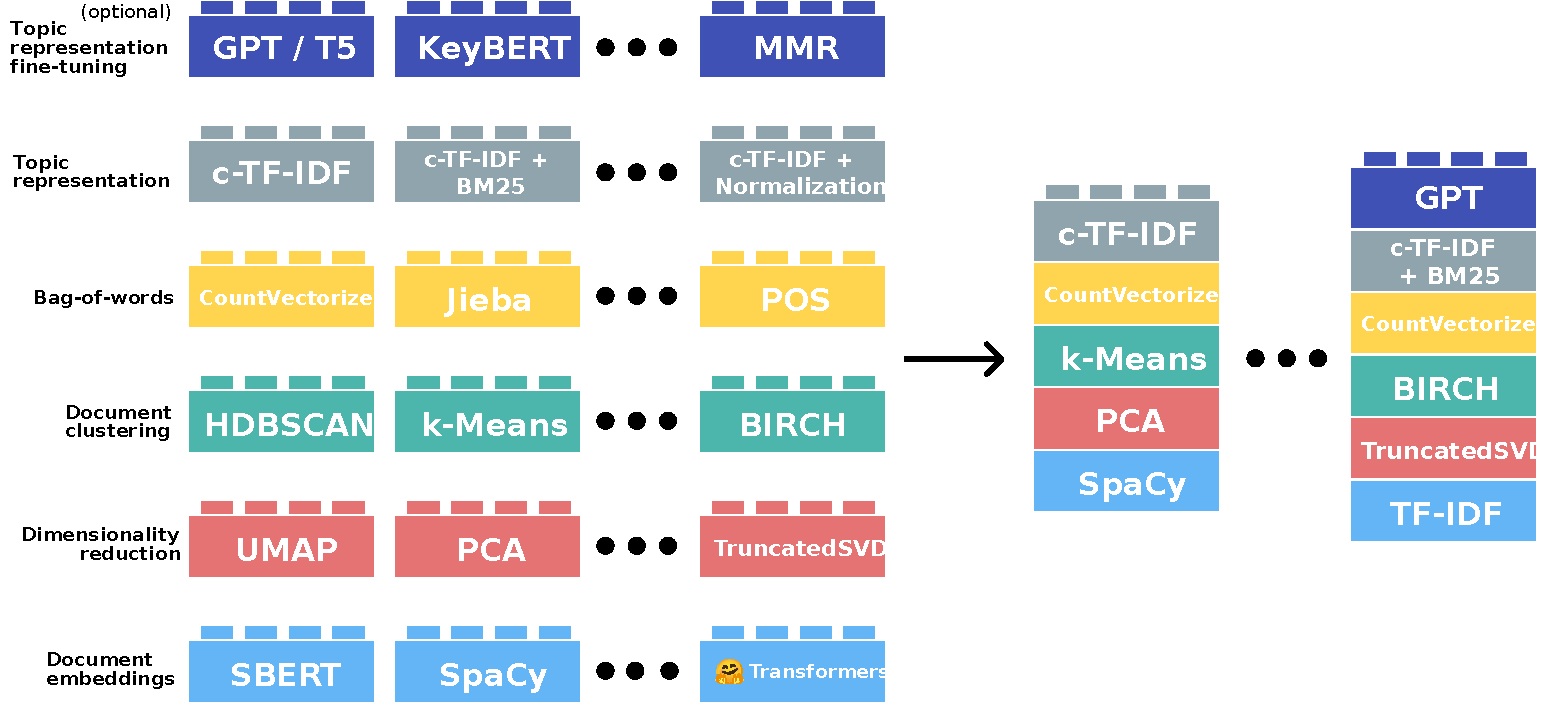
\includegraphics[width=\textwidth]{images/modularity_modified.pdf}
    \caption{BERTopic modularity (inspired by \cite{grootendorst_algorithm_nodate})}
    \label{fig:modularity_modified}
\end{figure}

\textbf{Document embeddings}

In BERTopic, documents are transformed into embeddings to create vector space representations for semantic comparison. It is based on the idea that documents sharing the same topic will have similar semantics. For this embedding step, BERTopic utilizes the SBERT framework \citet{reimers_sentence-bert_2019}. SBERT enables the conversion of sentences and paragraphs into dense vector representations by employing pre-trained language models. This achieves top performance on several sentence embedding tasks \cite{reimers_making_2020}. The embeddings are mainly used for clustering documents with semantic similarities rather than directly for topic generation. BERTopic can use any embedding technique, provided the language model used for generating document embeddings is fine-tuned for semantic similarity. Hence, the quality of BERTopic's clustering improves as more advanced language models are developed, allowing BERTopic to evolve alongside advancements in embedding techniques.

\textbf{Dimensionality reduction}

As the dimensionality of data increases, the distance to the nearest data point tends to become similar to the distance to the farthest data point \cite{aggarwal_surprising_2001, beyer_when_1999}. This phenomenon implies that in high-dimensional spaces, the notion of spatial locality becomes unclear, and distances between points show minimal variation. While several clustering methods have been developed to address the curse of dimensionality \cite{pandove_systematic_2018, steinbach_challenges_2004}, a simpler strategy involves reducing the dimensionality of embeddings. Although PCA and t-SNE are popular dimensionality reduction techniques, UMAP has been found to better preserve the local and global characteristics of high-dimensional data in its lower-dimensional representations \cite{mcinnes_umap_2020}. Furthermore, UMAP's flexibility regarding the dimensions of embeddings allows its application across various language models.

\textbf{Document clustering}

The reduced embeddings are clustered using HDBSCAN \cite{mcinnes_hdbscan_2017}. HDBSCAN is built on top of DBSCAN and is designed to identify clusters of various densities by transforming DBSCAN into a hierarchical clustering algorithm. It employs a soft-clustering approach, which allows for the treatment of noise as outliers. This method helps to prevent unrelated documents from being grouped into any cluster, which is expected to improve the quality of topic representations. Furthermore, \citet{allaoui_considerably_2020} showed that the performance of well-known clustering algorithms, including k-Means and HDBSCAN, can be significantly improved by reducing the dimensionality of high-dimensional embeddings with UMAP, in terms of both clustering accuracy and computational time.

\textbf{Bag-of-words}

Before creating topic representations in BERTopic, it is necessary to select a technique that supports the algorithm's modular nature. When using HDBSCAN, we assume that clusters may vary in density and shape, indicating that techniques based on centroid models may not be suitable. The desired method should ideally make minimal assumptions about the cluster structures.

The process begins by combining all documents within a cluster into a single document, which then represents the entire cluster. Subsequently, the frequency of each word within this single document is counted, resulting in a bag-of-words representation that reflects the word frequencies at the cluster level rather than the individual document level. The adoption of a bag-of-words approach ensures that no assumptions are made about the density and shape of the clusters. Additionally, this representation is L1-normalized to account for the varying sizes of clusters.

\textbf{Topic representation}

The classic TF-IDF \cite{joachims_probabilistic_1997} method combines term frequency and inverse document frequency to calculate a weight $W_{t,d}$ for term $t$ in document $d$ as follows:

$$ W_{t,d} = tf_{t,d} \cdot \log\left(\frac{N}{df_t}\right) $$

Here, term frequency $tf_{t,d}$ represents the frequency of term $t$ in document $d$, and inverse document frequency measures $t$'s importance across documents, calculated by the logarithm of the ratio of the total number of documents $N$ to the number of documents containing $t$.


BERTopic extends the TF-IDF concept to clusters of documents by introducing c-TF-IDF. In this approach, documents within a cluster are concatenated into a single document, and the TF-IDF formula is modified for cluster-level representation:

$$W_{t,c} = tf_{t,c} \cdot \log\left(1 + \frac{A}{tf_t}\right)$$

In this formula, term frequency $tf_{t,c}$ now models the frequency of term $t$ within a cluster $c$, treated as a single document. The inverse document frequency is substituted with an inverse class frequency, which assesses the term's importance to a cluster. This is calculated by the logarithm of the average number of words per cluster $A$ divided by the term's frequency $tf_t$ across all clusters, with $1$ added inside the logarithm to ensure positive values. This adaptation of TF-IDF to clusters allows us to model the importance of words in clusters instead of individual documents. Furthermore, by iteratively merging c-TF-IDF representations of less prevalent topics with their closest topics, the total number of topics can be reduced to meet a predefined threshold.

\textbf{(Optional) Topic representation fine-tuning}

After generating the c-TF-IDF representations, we obtain a collection of words that describe a collection of documents. c-TF-IDF is a method for quickly producing accurate topic representations. Nonetheless, the field of NLP is rapidly advancing, with frequent new developments. To make use of these developments, BERTopic offers the option to refine c-TF-IDF topics further using GPT, KeyBERT \cite{grootendorst_maartengrkeybert_2024}, spaCy \cite{noauthor_explosionspacy_nodate}, and other techniques, many of which are integrated within the BERTopic library.

In particular, the topics generated through c-TF-IDF can be viewed as canditate topics, comprising a set of keywords and representative documents. These can serve as a foundation for further refinement of topic representations. The availability of representative documents for each topic can be useful, as it enables fine-tuning on a reduced number of documents, thereby reducing computational demands. This makes the use of large models like GPT more viable in production environments, often resulting in shorter processing times compared to the steps of dimensionality reduction and clustering.

\subsubsection{Evaluation metrics}

According to \citet{abdelrazek_topic_2022}, topic models, which are applicable across a variety of domains, can undergo evaluation through two distinct approaches: extrinsic and intrinsic. Extrinsic evaluation assesses performance based on the specific domain of application, whereas intrinsic evaluation focuses on the qualities of the generated topics themselves, independent of any domain. This makes intrinsic evaluation more universally applicable. The various models are distinguished by their simplicity, computational efficiency, and underlying assumptions, which influence their performance across different corpora and applications. However, there is a lack of agreement on the criteria for evaluating topic models, and multiple methods exist for evaluating the same quality.

\citet{abdelrazek_topic_2022} highlight a range of criteria for evaluating topic models, including quality, interpretability, stability, diversity, efficiency, and flexibility, as illustrated in \cref{fig:evaluation_criteria}. We will focus on quality, interpretability, and diversity, given their relevance to our specific use case.

\begin{figure}[h] % adjust placement if needed
    \centering
    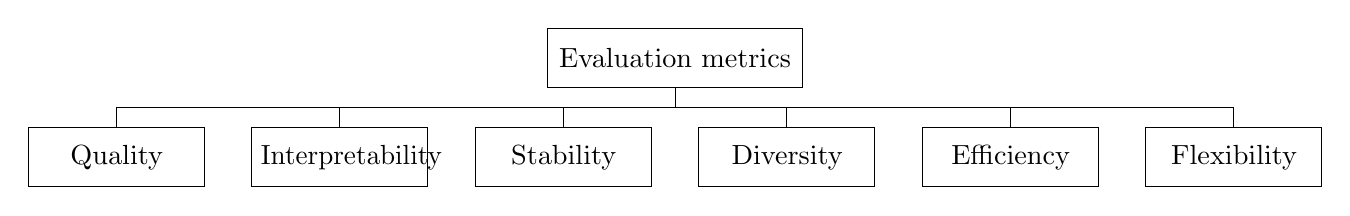
\begin{tikzpicture}
        \node (eval) [rectangle, draw, text width=3cm, text centered, minimum height=0.75cm] {Evaluation metrics};

        \node (quality) [rectangle, draw, below left=of eval, text width=2cm, text centered, minimum height=0.75cm, xshift=-3.35cm, yshift=0.5cm] {Quality};
        \node (interpretability) [rectangle, draw, right=of quality, text width=2cm, text centered, minimum height=0.75cm, xshift=-0.41cm] {Interpretability};
        \node (stability) [rectangle, draw, right=of interpretability, text width=2cm, text centered, minimum height=0.75cm, xshift=-0.41cm] {Stability};
        \node (diversity) [rectangle, draw, right=of stability, text width=2cm, text centered, minimum height=0.75cm, xshift=-0.41cm] {Diversity};
        \node (efficiency) [rectangle, draw, right=of diversity, text width=2cm, text centered, minimum height=0.75cm, xshift=-0.41cm] {Efficiency};
        \node (flexibility) [rectangle, draw, right=of efficiency, text width=2cm, text centered, minimum height=0.75cm, xshift=-0.41cm] {Flexibility};

        \draw[-] (eval.south) -- ++(0,-0.25) -| (quality.north);
        \draw[-] (eval.south) -- ++(0,-0.25) -| (interpretability.north);
        \draw[-] (eval.south) -- ++(0,-0.25) -| (stability.north);
        \draw[-] (eval.south) -- ++(0,-0.25) -| (diversity.north);
        \draw[-] (eval.south) -- ++(0,-0.25) -| (efficiency.north);
        \draw[-] (eval.south) -- ++(0,-0.25) -| (flexibility.north);
    \end{tikzpicture}
    \caption{Topic models evaluation criteria \cite{abdelrazek_topic_2022}}
    \label{fig:evaluation_criteria}
\end{figure}

\textbf{Quality and Perplexity}

Perplexity measures a model's ability to reproduce the documents in a corpus using the learned topics. It evaluates the model's predictive capability rather than its ability to uncover the latent structure, indicating how effectively the model explains the data. A lower perplexity suggests a model is more effective in explaining the observed documents, as it implies a higher information gain from predicting the outcome of the random variable.

However, using perplexity as an evaluation metric for our use case has several drawbacks. Firstly, perplexity needs to be normalized for the size of the corpus vocabulary, as it varies with different corpus and topic sizes. This is a consideration especially since BERTopic may not consistently extract the same number of topics without specific instructions to limit topic quantity. Additionally, perplexity has not been found to be correlated with human judgment \cite{chang_reading_2009}. Furthermore, non-generative models like NMF do not have a defined perplexity score because they do not provide probabilities of word sequences.

\textbf{Interpretability and Topic coherence}

A topic is defined as a discrete distribution over words, with the expectation that this word set is interpretable by humans. For interpretability, the words generated should collectively convey a single semantic meaning. Topic coherence metrics evaluate how related the top-k words of a topic are to one another.

\citet{newman_automatic_2010} measure coherence by examining the lexical similarity between word pairs, employing various similarity measures and identifying mutual information as the most reliably performing measure. The pointwise mutual information, $PMI$, between a pair of words $(w_i, w_j)$ is calculated as follows:

$$PMI(w_i, w_j) = \frac{\log p(w_i, w_j)}{p(w_i)p(w_j)}$$

This formula quantifies the difference between the probability of $w_i$ and $w_j$ occurring together compared to the probabilities of them appearing independently within the corpus. Here, $p(w_i,w_j)$ represents the joint probability of both words occurring together, while $p(w_i)$ and $p(w_j)$ are the individual probabilities $w_i$ and $w_j$ occurring in the corpus.

A known trade-off exists between coherence and perplexity \cite{chang_reading_2009}, where optimizing for lower perplexity often results in decreased coherence.

\textbf{Topic diversity}

Topic diversity refers to the semantic diversity among the generated topics. A method to assess diversity, as proposed by \citet{dieng_topic_2020}, considers it as the proportion of unique words within the top 25 words across all topics. So, in general, diversity metrics aim to quantify the variation among the top-k words within a topic. A high score in topic diversity suggests that a topic model successfully generates diverse topics, whereas a low score may indicate the presence of redundant topics, showing the model's inability to clearly differentiate the themes within the corpus. It is important to note that the choice of the number of topics in a model significantly influences topic diversity. Choosing too many topics might lead to similar topics with overlapping words, while too few topics can result in overly broad topics that lack interpretability.

\textbf{Classification evaluation metrics}

The evaluation metrics discussed previously pertain to topic modeling as an unsupervised learning task. If through experimentation we establish that the BERTopic model underperforms, we might approach the problem as a (semi-)supervised task, in which case different evaluation metrics would be used. Beyond well-known metrics such as accuracy, precision, recall, and F1 score, coverage and purity would also be considered \cite{churchill_evolution_2022}.

Coverage examines the extent to which the concepts within the document collection are captured by the model. It can be divided into topic coverage and document coverage. Topic coverage measures how good the model is at identifying the topics in a document corpus. The most popular measure for topic coverage is topic recall, which denotes the proportion of ground truth topics identified by the topic model. Conversely, document coverage focuses on how well documents are represented by the topics. Topic model accuracy is a frequently used measure, which is the proportion of documents accurately labeled by the model. For evaluating both topic recall and accuracy, ground truth topics are required.

When ground truth topics are missing, alternative metrics like purity are used. Purity measures the model's accuracy under the assumption that documents are always assigned to the dominant topic. This metric aims to penalize models that assign a large number of low probability topics to documents, in contrast to models that assign a high probability to a single topic from the document corpus.

\textbf{OCTIS}

OCTIS (Optimizing and Comparing Topic models Is Simple) \cite{terragni_octis_2021} is an open-source framework for the training, analysis, and comparison of topic models across various datasets and evaluation metrics.

It allows for the optimization of model hyper-parameters for experimental comparison. OCTIS introduces a pipeline for topic modeling (\cref{fig:octis}), which includes dataset preprocessing, training topic models, evaluation metrics, hyperparameter optimization, and visualization through an interactive web dashboard.

OCTIS offers a range of evaluation metrics for assessing topic models, such as coherence, significance, diversity, and classification metrics.

The discovery of optimal hyper-parameter settings relies on a Bayesian Optimization (BO) approach \cite{archetti_bayesian_2019, galuzzi_hyperparameter_2020, snoek_practical_2012}, where the objective can be any of the available evaluation metrics. Given the potential variability in performance outcomes due to noise, the objective function is defined as the median performance across multiple runs of the model under the same hyperparameter settings for the chosen evaluation metric.

BO is a sequential, model-based optimization technique for noisy black-box functions that are costly and complex to evaluate directly, such as topic models. Its main idea involves using all previously evaluated hyperparameter settings to approximate the performance metric's value, and then selecting new, likely better hyperparameter settings for the next run. The approximation is done by a probabilistic \textit{surrogate model}, which has a prior belief of the objective function based on observed hyperparameter settings. The selection of the next hyperparameter settings is driven by optimizing an \textit{acquisition function}, which uses the uncertainty within the posterior distribution to guide the exploration of the parameter space.

\begin{figure}[h] % adjust placement if needed
    \centering
    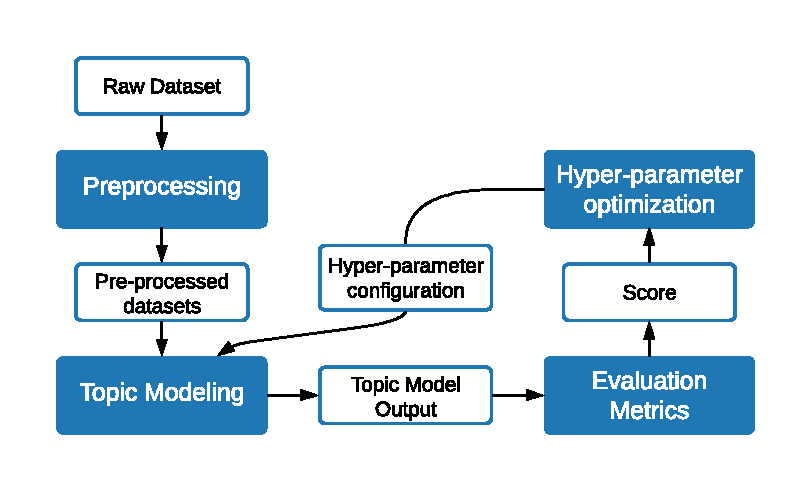
\includegraphics[width=0.7\textwidth]{images/octis.pdf}
    \caption{Workflow of the OCTIS framework \cite{terragni_octis_2021}}
    \label{fig:octis}
\end{figure}

OCTIS could be useful for the Master's thesis, as it provides a unified framework for training the proposed BERTopic model alongside the baseline models, facilitating their comparison across a variety of evaluation metrics. In fact, in the original BERTopic paper, \citet{grootendorst_bertopic_2022} employed OCTIS to evaluate the model's performance.

% \todo[inline]{

%     - Go deeper into the models that will be used. I.e., BERTopic.

%     - Discuss metrics more in depth.

%     - Discuss baselines - LDA, T2V, NMF. What could be some other baselines?

%     Taniya:
%     - For baselines, we can refer to the papers and include models which are generally used as a baseline (for easy comparison)>
%     so LDA, T2V, NMF, etc.
% }

\subsection{Preliminary studies and analyses}
% {
% \color{red}
% This subsection can be used to show any designs, developments, outcomes and tangible results that you may have obtained in the initial part of the MSc project, and/or any other type of evidence to suggest that your research can succeed during the continuation.

% In Figure~\ref{fig:2}, we show that our results are promising, even though they have no relation to the rest of the text here and are presented only as an example of a figure. You should use any type of visual aide available to support your studies and analyses.
% \begin{figure}[htp]
% \centering
%  \begin{tabular}{r}
% 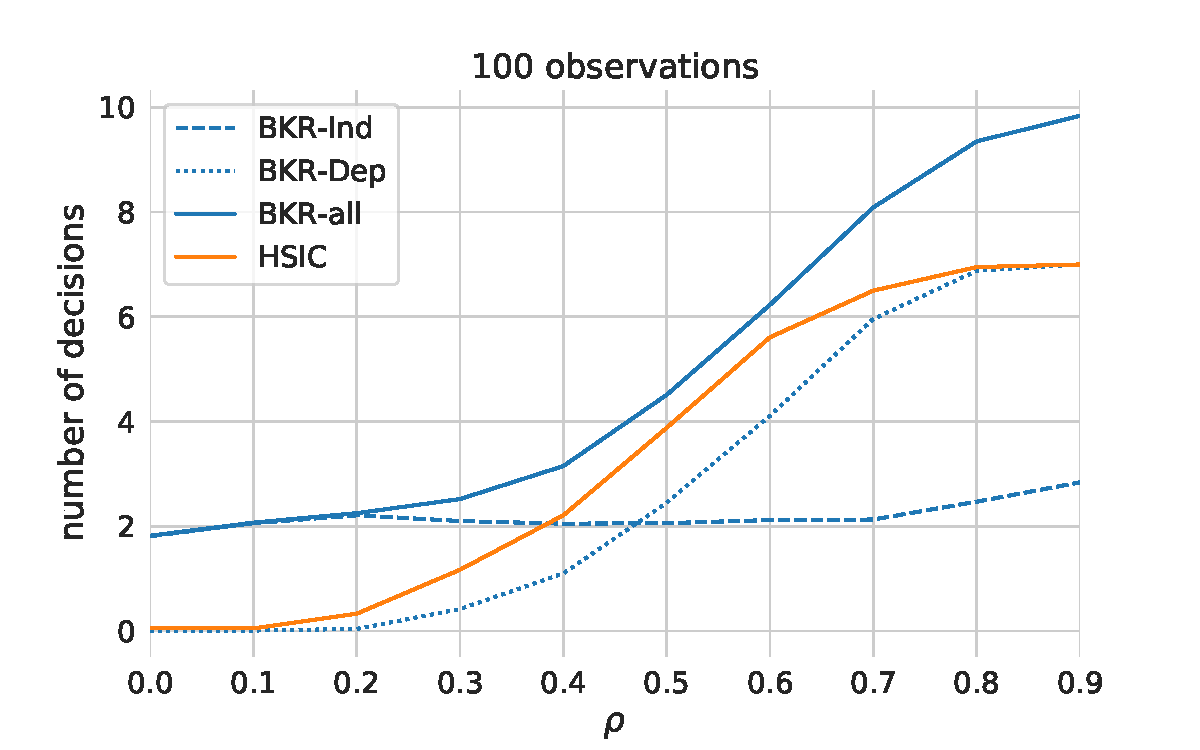
\includegraphics[height=1.9in]{100.pdf}
% 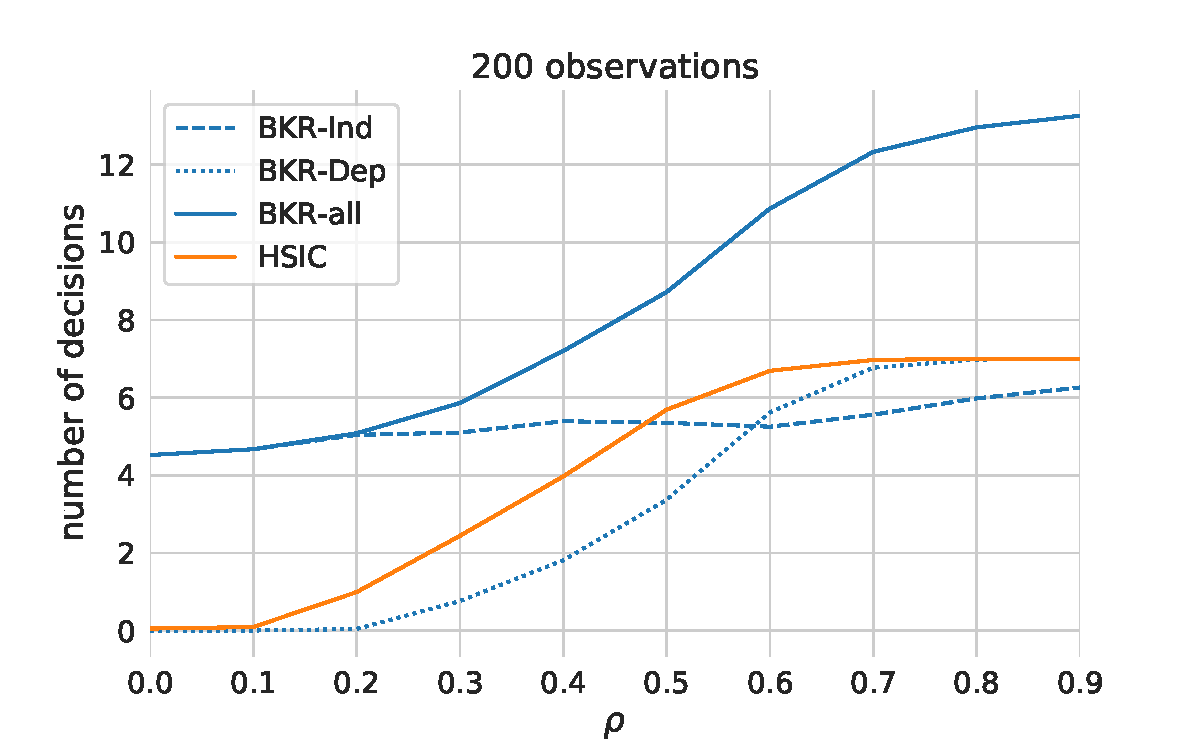
\includegraphics[height=1.9in]{200.pdf}
% \end{tabular}
% \caption{Synthetic dataset D1. \textbf{Just an example of figures.}}
% \label{fig:2}
% \end{figure}
% }

Two initial developments illustrate the potential of the Master's thesis. The first approach, by \citeauthor{das_openmlscripts_nodate} \cite{das_openmlscripts_nodate}, employs OpenML's dataset descriptions along with GPT-3.5-turbo for dataset tagging. The second development utilized BERTopic, primarily with default parameters.

\subsubsection{Tag assignment using GPT 3.5}

Previous research by \citeauthor{das_openmlscripts_nodate} has explored the automation of dataset tagging on OpenML using GPT-3.5-turbo for assigning semantic tags based on dataset descriptions and a set list of tags. \citeauthor{das_openmlscripts_nodate}'s approach demonstrated the feasibility of classifying datasets with a set of predefined tags, similar to the dataset tags in the Wolfram Data Repository \cite{noauthor_wolfram_nodate}.

Specifically, the predefined tags were - \textit{Agriculture}, \textit{Astronomy}, \textit{Chemistry}, \textit{Computational Universe}, \textit{Computer Systems}, \textit{Culture}, \textit{Demographics}, \textit{Earth Science}, \textit{Economics}, \textit{Education}, \textit{Geography}, \textit{Government}, \textit{Health}, \textit{History}, \textit{Human Activities}, \textit{Images}, \textit{Language}, \textit{Life Science}, \textit{Machine Learning}, \textit{Manufacturing}, \textit{Mathematics}, \textit{Medicine}, \textit{Meteorology}, \textit{Physical Sciences}, \textit{Politics}, \textit{Social Media}, \textit{Sociology}, \textit{Statistics}, \textit{Text \& Literature}, \textit{Transportation}

To illustrate the potential of using language models for automated dataset classification, the researcher developed a Python script that utilized the OpenAI GPT-3.5-turbo API and spaCy's natural language processing library. The script downloaded the descriptions of all datasets available on OpenML and used the GPT-3.5-turbo API to generate semantic tags for each dataset based on its description and the predefined list of tags.

To process the generated tags, the script employed spaCy to clean and standardize the tags, ensuring that they matched the predefined list of tags. While the script did not include an evaluation of the automated tagging system, it demonstrated the feasibility of using language models for dataset classification and the potential for improving the efficiency of the tagging process.

\cref{table:tag-occurrence} demonstrates the distribution of semantic tags across the OpenML datasets, where "Machine Learning" is the most prevalent tag with a percentage of 20.72\%, followed by "Life Science" at 16.22\%, and "Chemistry" at 12.87\%. These tags indicate the primary areas of focus within the dataset, highlighting the significant emphasis on machine learning techniques, life science research, and chemical studies.

\begin{table}[htb]
    \caption{Percentage of occurrence for each tag}
    \begin{subtable}{.5\textwidth}
        \centering
        \begin{tabular}{@{\extracolsep{4pt}}lc}
            \toprule
            \textbf{Tag}       & \multicolumn{1}{c}{\textbf{Percentage (\%)}} \\
            \midrule
            Manufacturing      & 1.45                                         \\
            Machine Learning   & 20.72                                        \\
            Mathematics        & 2.69                                         \\
            Economics          & 5.01                                         \\
            Education          & 0.93                                         \\
            Medicine           & 2.88                                         \\
            Images             & 1.99                                         \\
            Health             & 2.35                                         \\
            Demographics       & 2.77                                         \\
            Life Science       & 16.22                                        \\
            Agriculture        & 1.05                                         \\
            Statistics         & 5.26                                         \\
            Human Activities   & 0.41                                         \\
            Physical Sciences  & 0.72                                         \\
            Chemistry          & 12.87                                        \\
            Text \& Literature & 0.55                                         \\
            \hline                                                            \\
        \end{tabular}
    \end{subtable}%
    \begin{subtable}{.5\textwidth}
        \centering
        \begin{tabular}{@{\extracolsep{4pt}}lc}
            \toprule
            \textbf{Tag}           & \multicolumn{1}{c}{\textbf{Percentage (\%)}} \\
            \midrule
            Transportation         & 2.35                                         \\
            Government             & 1.27                                         \\
            Politics               & 0.19                                         \\
            No description         & 2.55                                         \\
            Computer Systems       & 7.62                                         \\
            Astronomy              & 0.67                                         \\
            Earth Science          & 1.12                                         \\
            Social Media           & 2.07                                         \\
            Meteorology            & 1.40                                         \\
            Geography              & 0.99                                         \\
            Language               & 0.46                                         \\
            Computational Universe & 0.90                                         \\
            History                & 0.12                                         \\
            Culture                & 0.17                                         \\
            Sociology              & 0.22                                         \\
            \hline                                                                \\
        \end{tabular}
    \end{subtable}
    \label{table:tag-occurrence}
\end{table}


\subsubsection{Topic modeling proof of concept using BERTopic}

The second stage involved utilizing BERTopic to assess the feasibility of topic extraction. BERTopic was applied in an unsupervised manner to identify latent topics within the dataset descriptions.

Initial cleaning of the datasets involved removing those without descriptions, those with descriptions shorter than 100 characters, and those with repeated dataset descriptions. Datasets with identical descriptions typically represented different versions of the same dataset, where the descriptions did not vary between versions. It should be highlighted that while some datasets do update their descriptions across versions, in the majority of cases, descriptions were very similar.

\Cref{fig:description_length_histogram} illustrates the distribution of description lengths by character count. It reveals that most datasets have descriptions under 2000 characters. This observation is not seen as a limitation, given the successful application of topic models on brief texts, such as tweets, in previous studies.

\begin{figure}[h] % adjust placement if needed
    \centering
    %% Creator: Matplotlib, PGF backend
%%
%% To include the figure in your LaTeX document, write
%%   \input{<filename>.pgf}
%%
%% Make sure the required packages are loaded in your preamble
%%   \usepackage{pgf}
%%
%% Also ensure that all the required font packages are loaded; for instance,
%% the lmodern package is sometimes necessary when using math font.
%%   \usepackage{lmodern}
%%
%% Figures using additional raster images can only be included by \input if
%% they are in the same directory as the main LaTeX file. For loading figures
%% from other directories you can use the `import` package
%%   \usepackage{import}
%%
%% and then include the figures with
%%   \import{<path to file>}{<filename>.pgf}
%%
%% Matplotlib used the following preamble
%%   \def\mathdefault#1{#1}
%%   \everymath=\expandafter{\the\everymath\displaystyle}
%%   
%%   \makeatletter\@ifpackageloaded{underscore}{}{\usepackage[strings]{underscore}}\makeatother
%%
\begingroup%
\makeatletter%
\begin{pgfpicture}%
\pgfpathrectangle{\pgfpointorigin}{\pgfqpoint{4.650000in}{3.000000in}}%
\pgfusepath{use as bounding box, clip}%
\begin{pgfscope}%
\pgfsetbuttcap%
\pgfsetmiterjoin%
\definecolor{currentfill}{rgb}{1.000000,1.000000,1.000000}%
\pgfsetfillcolor{currentfill}%
\pgfsetlinewidth{0.000000pt}%
\definecolor{currentstroke}{rgb}{1.000000,1.000000,1.000000}%
\pgfsetstrokecolor{currentstroke}%
\pgfsetdash{}{0pt}%
\pgfpathmoveto{\pgfqpoint{0.000000in}{0.000000in}}%
\pgfpathlineto{\pgfqpoint{4.650000in}{0.000000in}}%
\pgfpathlineto{\pgfqpoint{4.650000in}{3.000000in}}%
\pgfpathlineto{\pgfqpoint{0.000000in}{3.000000in}}%
\pgfpathlineto{\pgfqpoint{0.000000in}{0.000000in}}%
\pgfpathclose%
\pgfusepath{fill}%
\end{pgfscope}%
\begin{pgfscope}%
\pgfsetbuttcap%
\pgfsetmiterjoin%
\definecolor{currentfill}{rgb}{1.000000,1.000000,1.000000}%
\pgfsetfillcolor{currentfill}%
\pgfsetlinewidth{0.000000pt}%
\definecolor{currentstroke}{rgb}{0.000000,0.000000,0.000000}%
\pgfsetstrokecolor{currentstroke}%
\pgfsetstrokeopacity{0.000000}%
\pgfsetdash{}{0pt}%
\pgfpathmoveto{\pgfqpoint{0.581250in}{0.450000in}}%
\pgfpathlineto{\pgfqpoint{4.185000in}{0.450000in}}%
\pgfpathlineto{\pgfqpoint{4.185000in}{2.640000in}}%
\pgfpathlineto{\pgfqpoint{0.581250in}{2.640000in}}%
\pgfpathlineto{\pgfqpoint{0.581250in}{0.450000in}}%
\pgfpathclose%
\pgfusepath{fill}%
\end{pgfscope}%
\begin{pgfscope}%
\pgfpathrectangle{\pgfqpoint{0.581250in}{0.450000in}}{\pgfqpoint{3.603750in}{2.190000in}}%
\pgfusepath{clip}%
\pgfsetbuttcap%
\pgfsetmiterjoin%
\definecolor{currentfill}{rgb}{0.121569,0.466667,0.705882}%
\pgfsetfillcolor{currentfill}%
\pgfsetlinewidth{0.000000pt}%
\definecolor{currentstroke}{rgb}{0.000000,0.000000,0.000000}%
\pgfsetstrokecolor{currentstroke}%
\pgfsetstrokeopacity{0.000000}%
\pgfsetdash{}{0pt}%
\pgfpathmoveto{\pgfqpoint{0.745057in}{0.450000in}}%
\pgfpathlineto{\pgfqpoint{0.777818in}{0.450000in}}%
\pgfpathlineto{\pgfqpoint{0.777818in}{0.778814in}}%
\pgfpathlineto{\pgfqpoint{0.745057in}{0.778814in}}%
\pgfpathlineto{\pgfqpoint{0.745057in}{0.450000in}}%
\pgfpathclose%
\pgfusepath{fill}%
\end{pgfscope}%
\begin{pgfscope}%
\pgfpathrectangle{\pgfqpoint{0.581250in}{0.450000in}}{\pgfqpoint{3.603750in}{2.190000in}}%
\pgfusepath{clip}%
\pgfsetbuttcap%
\pgfsetmiterjoin%
\definecolor{currentfill}{rgb}{0.121569,0.466667,0.705882}%
\pgfsetfillcolor{currentfill}%
\pgfsetlinewidth{0.000000pt}%
\definecolor{currentstroke}{rgb}{0.000000,0.000000,0.000000}%
\pgfsetstrokecolor{currentstroke}%
\pgfsetstrokeopacity{0.000000}%
\pgfsetdash{}{0pt}%
\pgfpathmoveto{\pgfqpoint{0.777818in}{0.450000in}}%
\pgfpathlineto{\pgfqpoint{0.810580in}{0.450000in}}%
\pgfpathlineto{\pgfqpoint{0.810580in}{1.233352in}}%
\pgfpathlineto{\pgfqpoint{0.777818in}{1.233352in}}%
\pgfpathlineto{\pgfqpoint{0.777818in}{0.450000in}}%
\pgfpathclose%
\pgfusepath{fill}%
\end{pgfscope}%
\begin{pgfscope}%
\pgfpathrectangle{\pgfqpoint{0.581250in}{0.450000in}}{\pgfqpoint{3.603750in}{2.190000in}}%
\pgfusepath{clip}%
\pgfsetbuttcap%
\pgfsetmiterjoin%
\definecolor{currentfill}{rgb}{0.121569,0.466667,0.705882}%
\pgfsetfillcolor{currentfill}%
\pgfsetlinewidth{0.000000pt}%
\definecolor{currentstroke}{rgb}{0.000000,0.000000,0.000000}%
\pgfsetstrokecolor{currentstroke}%
\pgfsetstrokeopacity{0.000000}%
\pgfsetdash{}{0pt}%
\pgfpathmoveto{\pgfqpoint{0.810580in}{0.450000in}}%
\pgfpathlineto{\pgfqpoint{0.843341in}{0.450000in}}%
\pgfpathlineto{\pgfqpoint{0.843341in}{0.840064in}}%
\pgfpathlineto{\pgfqpoint{0.810580in}{0.840064in}}%
\pgfpathlineto{\pgfqpoint{0.810580in}{0.450000in}}%
\pgfpathclose%
\pgfusepath{fill}%
\end{pgfscope}%
\begin{pgfscope}%
\pgfpathrectangle{\pgfqpoint{0.581250in}{0.450000in}}{\pgfqpoint{3.603750in}{2.190000in}}%
\pgfusepath{clip}%
\pgfsetbuttcap%
\pgfsetmiterjoin%
\definecolor{currentfill}{rgb}{0.121569,0.466667,0.705882}%
\pgfsetfillcolor{currentfill}%
\pgfsetlinewidth{0.000000pt}%
\definecolor{currentstroke}{rgb}{0.000000,0.000000,0.000000}%
\pgfsetstrokecolor{currentstroke}%
\pgfsetstrokeopacity{0.000000}%
\pgfsetdash{}{0pt}%
\pgfpathmoveto{\pgfqpoint{0.843341in}{0.450000in}}%
\pgfpathlineto{\pgfqpoint{0.876102in}{0.450000in}}%
\pgfpathlineto{\pgfqpoint{0.876102in}{0.764308in}}%
\pgfpathlineto{\pgfqpoint{0.843341in}{0.764308in}}%
\pgfpathlineto{\pgfqpoint{0.843341in}{0.450000in}}%
\pgfpathclose%
\pgfusepath{fill}%
\end{pgfscope}%
\begin{pgfscope}%
\pgfpathrectangle{\pgfqpoint{0.581250in}{0.450000in}}{\pgfqpoint{3.603750in}{2.190000in}}%
\pgfusepath{clip}%
\pgfsetbuttcap%
\pgfsetmiterjoin%
\definecolor{currentfill}{rgb}{0.121569,0.466667,0.705882}%
\pgfsetfillcolor{currentfill}%
\pgfsetlinewidth{0.000000pt}%
\definecolor{currentstroke}{rgb}{0.000000,0.000000,0.000000}%
\pgfsetstrokecolor{currentstroke}%
\pgfsetstrokeopacity{0.000000}%
\pgfsetdash{}{0pt}%
\pgfpathmoveto{\pgfqpoint{0.876102in}{0.450000in}}%
\pgfpathlineto{\pgfqpoint{0.908864in}{0.450000in}}%
\pgfpathlineto{\pgfqpoint{0.908864in}{2.535714in}}%
\pgfpathlineto{\pgfqpoint{0.876102in}{2.535714in}}%
\pgfpathlineto{\pgfqpoint{0.876102in}{0.450000in}}%
\pgfpathclose%
\pgfusepath{fill}%
\end{pgfscope}%
\begin{pgfscope}%
\pgfpathrectangle{\pgfqpoint{0.581250in}{0.450000in}}{\pgfqpoint{3.603750in}{2.190000in}}%
\pgfusepath{clip}%
\pgfsetbuttcap%
\pgfsetmiterjoin%
\definecolor{currentfill}{rgb}{0.121569,0.466667,0.705882}%
\pgfsetfillcolor{currentfill}%
\pgfsetlinewidth{0.000000pt}%
\definecolor{currentstroke}{rgb}{0.000000,0.000000,0.000000}%
\pgfsetstrokecolor{currentstroke}%
\pgfsetstrokeopacity{0.000000}%
\pgfsetdash{}{0pt}%
\pgfpathmoveto{\pgfqpoint{0.908864in}{0.450000in}}%
\pgfpathlineto{\pgfqpoint{0.941625in}{0.450000in}}%
\pgfpathlineto{\pgfqpoint{0.941625in}{0.659539in}}%
\pgfpathlineto{\pgfqpoint{0.908864in}{0.659539in}}%
\pgfpathlineto{\pgfqpoint{0.908864in}{0.450000in}}%
\pgfpathclose%
\pgfusepath{fill}%
\end{pgfscope}%
\begin{pgfscope}%
\pgfpathrectangle{\pgfqpoint{0.581250in}{0.450000in}}{\pgfqpoint{3.603750in}{2.190000in}}%
\pgfusepath{clip}%
\pgfsetbuttcap%
\pgfsetmiterjoin%
\definecolor{currentfill}{rgb}{0.121569,0.466667,0.705882}%
\pgfsetfillcolor{currentfill}%
\pgfsetlinewidth{0.000000pt}%
\definecolor{currentstroke}{rgb}{0.000000,0.000000,0.000000}%
\pgfsetstrokecolor{currentstroke}%
\pgfsetstrokeopacity{0.000000}%
\pgfsetdash{}{0pt}%
\pgfpathmoveto{\pgfqpoint{0.941625in}{0.450000in}}%
\pgfpathlineto{\pgfqpoint{0.974386in}{0.450000in}}%
\pgfpathlineto{\pgfqpoint{0.974386in}{0.656315in}}%
\pgfpathlineto{\pgfqpoint{0.941625in}{0.656315in}}%
\pgfpathlineto{\pgfqpoint{0.941625in}{0.450000in}}%
\pgfpathclose%
\pgfusepath{fill}%
\end{pgfscope}%
\begin{pgfscope}%
\pgfpathrectangle{\pgfqpoint{0.581250in}{0.450000in}}{\pgfqpoint{3.603750in}{2.190000in}}%
\pgfusepath{clip}%
\pgfsetbuttcap%
\pgfsetmiterjoin%
\definecolor{currentfill}{rgb}{0.121569,0.466667,0.705882}%
\pgfsetfillcolor{currentfill}%
\pgfsetlinewidth{0.000000pt}%
\definecolor{currentstroke}{rgb}{0.000000,0.000000,0.000000}%
\pgfsetstrokecolor{currentstroke}%
\pgfsetstrokeopacity{0.000000}%
\pgfsetdash{}{0pt}%
\pgfpathmoveto{\pgfqpoint{0.974386in}{0.450000in}}%
\pgfpathlineto{\pgfqpoint{1.007148in}{0.450000in}}%
\pgfpathlineto{\pgfqpoint{1.007148in}{0.595065in}}%
\pgfpathlineto{\pgfqpoint{0.974386in}{0.595065in}}%
\pgfpathlineto{\pgfqpoint{0.974386in}{0.450000in}}%
\pgfpathclose%
\pgfusepath{fill}%
\end{pgfscope}%
\begin{pgfscope}%
\pgfpathrectangle{\pgfqpoint{0.581250in}{0.450000in}}{\pgfqpoint{3.603750in}{2.190000in}}%
\pgfusepath{clip}%
\pgfsetbuttcap%
\pgfsetmiterjoin%
\definecolor{currentfill}{rgb}{0.121569,0.466667,0.705882}%
\pgfsetfillcolor{currentfill}%
\pgfsetlinewidth{0.000000pt}%
\definecolor{currentstroke}{rgb}{0.000000,0.000000,0.000000}%
\pgfsetstrokecolor{currentstroke}%
\pgfsetstrokeopacity{0.000000}%
\pgfsetdash{}{0pt}%
\pgfpathmoveto{\pgfqpoint{1.007148in}{0.450000in}}%
\pgfpathlineto{\pgfqpoint{1.039909in}{0.450000in}}%
\pgfpathlineto{\pgfqpoint{1.039909in}{0.632137in}}%
\pgfpathlineto{\pgfqpoint{1.007148in}{0.632137in}}%
\pgfpathlineto{\pgfqpoint{1.007148in}{0.450000in}}%
\pgfpathclose%
\pgfusepath{fill}%
\end{pgfscope}%
\begin{pgfscope}%
\pgfpathrectangle{\pgfqpoint{0.581250in}{0.450000in}}{\pgfqpoint{3.603750in}{2.190000in}}%
\pgfusepath{clip}%
\pgfsetbuttcap%
\pgfsetmiterjoin%
\definecolor{currentfill}{rgb}{0.121569,0.466667,0.705882}%
\pgfsetfillcolor{currentfill}%
\pgfsetlinewidth{0.000000pt}%
\definecolor{currentstroke}{rgb}{0.000000,0.000000,0.000000}%
\pgfsetstrokecolor{currentstroke}%
\pgfsetstrokeopacity{0.000000}%
\pgfsetdash{}{0pt}%
\pgfpathmoveto{\pgfqpoint{1.039909in}{0.450000in}}%
\pgfpathlineto{\pgfqpoint{1.072670in}{0.450000in}}%
\pgfpathlineto{\pgfqpoint{1.072670in}{0.564440in}}%
\pgfpathlineto{\pgfqpoint{1.039909in}{0.564440in}}%
\pgfpathlineto{\pgfqpoint{1.039909in}{0.450000in}}%
\pgfpathclose%
\pgfusepath{fill}%
\end{pgfscope}%
\begin{pgfscope}%
\pgfpathrectangle{\pgfqpoint{0.581250in}{0.450000in}}{\pgfqpoint{3.603750in}{2.190000in}}%
\pgfusepath{clip}%
\pgfsetbuttcap%
\pgfsetmiterjoin%
\definecolor{currentfill}{rgb}{0.121569,0.466667,0.705882}%
\pgfsetfillcolor{currentfill}%
\pgfsetlinewidth{0.000000pt}%
\definecolor{currentstroke}{rgb}{0.000000,0.000000,0.000000}%
\pgfsetstrokecolor{currentstroke}%
\pgfsetstrokeopacity{0.000000}%
\pgfsetdash{}{0pt}%
\pgfpathmoveto{\pgfqpoint{1.072670in}{0.450000in}}%
\pgfpathlineto{\pgfqpoint{1.105432in}{0.450000in}}%
\pgfpathlineto{\pgfqpoint{1.105432in}{0.725624in}}%
\pgfpathlineto{\pgfqpoint{1.072670in}{0.725624in}}%
\pgfpathlineto{\pgfqpoint{1.072670in}{0.450000in}}%
\pgfpathclose%
\pgfusepath{fill}%
\end{pgfscope}%
\begin{pgfscope}%
\pgfpathrectangle{\pgfqpoint{0.581250in}{0.450000in}}{\pgfqpoint{3.603750in}{2.190000in}}%
\pgfusepath{clip}%
\pgfsetbuttcap%
\pgfsetmiterjoin%
\definecolor{currentfill}{rgb}{0.121569,0.466667,0.705882}%
\pgfsetfillcolor{currentfill}%
\pgfsetlinewidth{0.000000pt}%
\definecolor{currentstroke}{rgb}{0.000000,0.000000,0.000000}%
\pgfsetstrokecolor{currentstroke}%
\pgfsetstrokeopacity{0.000000}%
\pgfsetdash{}{0pt}%
\pgfpathmoveto{\pgfqpoint{1.105432in}{0.450000in}}%
\pgfpathlineto{\pgfqpoint{1.138193in}{0.450000in}}%
\pgfpathlineto{\pgfqpoint{1.138193in}{0.667598in}}%
\pgfpathlineto{\pgfqpoint{1.105432in}{0.667598in}}%
\pgfpathlineto{\pgfqpoint{1.105432in}{0.450000in}}%
\pgfpathclose%
\pgfusepath{fill}%
\end{pgfscope}%
\begin{pgfscope}%
\pgfpathrectangle{\pgfqpoint{0.581250in}{0.450000in}}{\pgfqpoint{3.603750in}{2.190000in}}%
\pgfusepath{clip}%
\pgfsetbuttcap%
\pgfsetmiterjoin%
\definecolor{currentfill}{rgb}{0.121569,0.466667,0.705882}%
\pgfsetfillcolor{currentfill}%
\pgfsetlinewidth{0.000000pt}%
\definecolor{currentstroke}{rgb}{0.000000,0.000000,0.000000}%
\pgfsetstrokecolor{currentstroke}%
\pgfsetstrokeopacity{0.000000}%
\pgfsetdash{}{0pt}%
\pgfpathmoveto{\pgfqpoint{1.138193in}{0.450000in}}%
\pgfpathlineto{\pgfqpoint{1.170955in}{0.450000in}}%
\pgfpathlineto{\pgfqpoint{1.170955in}{0.659539in}}%
\pgfpathlineto{\pgfqpoint{1.138193in}{0.659539in}}%
\pgfpathlineto{\pgfqpoint{1.138193in}{0.450000in}}%
\pgfpathclose%
\pgfusepath{fill}%
\end{pgfscope}%
\begin{pgfscope}%
\pgfpathrectangle{\pgfqpoint{0.581250in}{0.450000in}}{\pgfqpoint{3.603750in}{2.190000in}}%
\pgfusepath{clip}%
\pgfsetbuttcap%
\pgfsetmiterjoin%
\definecolor{currentfill}{rgb}{0.121569,0.466667,0.705882}%
\pgfsetfillcolor{currentfill}%
\pgfsetlinewidth{0.000000pt}%
\definecolor{currentstroke}{rgb}{0.000000,0.000000,0.000000}%
\pgfsetstrokecolor{currentstroke}%
\pgfsetstrokeopacity{0.000000}%
\pgfsetdash{}{0pt}%
\pgfpathmoveto{\pgfqpoint{1.170955in}{0.450000in}}%
\pgfpathlineto{\pgfqpoint{1.203716in}{0.450000in}}%
\pgfpathlineto{\pgfqpoint{1.203716in}{0.508026in}}%
\pgfpathlineto{\pgfqpoint{1.170955in}{0.508026in}}%
\pgfpathlineto{\pgfqpoint{1.170955in}{0.450000in}}%
\pgfpathclose%
\pgfusepath{fill}%
\end{pgfscope}%
\begin{pgfscope}%
\pgfpathrectangle{\pgfqpoint{0.581250in}{0.450000in}}{\pgfqpoint{3.603750in}{2.190000in}}%
\pgfusepath{clip}%
\pgfsetbuttcap%
\pgfsetmiterjoin%
\definecolor{currentfill}{rgb}{0.121569,0.466667,0.705882}%
\pgfsetfillcolor{currentfill}%
\pgfsetlinewidth{0.000000pt}%
\definecolor{currentstroke}{rgb}{0.000000,0.000000,0.000000}%
\pgfsetstrokecolor{currentstroke}%
\pgfsetstrokeopacity{0.000000}%
\pgfsetdash{}{0pt}%
\pgfpathmoveto{\pgfqpoint{1.203716in}{0.450000in}}%
\pgfpathlineto{\pgfqpoint{1.236477in}{0.450000in}}%
\pgfpathlineto{\pgfqpoint{1.236477in}{0.495131in}}%
\pgfpathlineto{\pgfqpoint{1.203716in}{0.495131in}}%
\pgfpathlineto{\pgfqpoint{1.203716in}{0.450000in}}%
\pgfpathclose%
\pgfusepath{fill}%
\end{pgfscope}%
\begin{pgfscope}%
\pgfpathrectangle{\pgfqpoint{0.581250in}{0.450000in}}{\pgfqpoint{3.603750in}{2.190000in}}%
\pgfusepath{clip}%
\pgfsetbuttcap%
\pgfsetmiterjoin%
\definecolor{currentfill}{rgb}{0.121569,0.466667,0.705882}%
\pgfsetfillcolor{currentfill}%
\pgfsetlinewidth{0.000000pt}%
\definecolor{currentstroke}{rgb}{0.000000,0.000000,0.000000}%
\pgfsetstrokecolor{currentstroke}%
\pgfsetstrokeopacity{0.000000}%
\pgfsetdash{}{0pt}%
\pgfpathmoveto{\pgfqpoint{1.236477in}{0.450000in}}%
\pgfpathlineto{\pgfqpoint{1.269239in}{0.450000in}}%
\pgfpathlineto{\pgfqpoint{1.269239in}{1.222069in}}%
\pgfpathlineto{\pgfqpoint{1.236477in}{1.222069in}}%
\pgfpathlineto{\pgfqpoint{1.236477in}{0.450000in}}%
\pgfpathclose%
\pgfusepath{fill}%
\end{pgfscope}%
\begin{pgfscope}%
\pgfpathrectangle{\pgfqpoint{0.581250in}{0.450000in}}{\pgfqpoint{3.603750in}{2.190000in}}%
\pgfusepath{clip}%
\pgfsetbuttcap%
\pgfsetmiterjoin%
\definecolor{currentfill}{rgb}{0.121569,0.466667,0.705882}%
\pgfsetfillcolor{currentfill}%
\pgfsetlinewidth{0.000000pt}%
\definecolor{currentstroke}{rgb}{0.000000,0.000000,0.000000}%
\pgfsetstrokecolor{currentstroke}%
\pgfsetstrokeopacity{0.000000}%
\pgfsetdash{}{0pt}%
\pgfpathmoveto{\pgfqpoint{1.269239in}{0.450000in}}%
\pgfpathlineto{\pgfqpoint{1.302000in}{0.450000in}}%
\pgfpathlineto{\pgfqpoint{1.302000in}{0.606348in}}%
\pgfpathlineto{\pgfqpoint{1.269239in}{0.606348in}}%
\pgfpathlineto{\pgfqpoint{1.269239in}{0.450000in}}%
\pgfpathclose%
\pgfusepath{fill}%
\end{pgfscope}%
\begin{pgfscope}%
\pgfpathrectangle{\pgfqpoint{0.581250in}{0.450000in}}{\pgfqpoint{3.603750in}{2.190000in}}%
\pgfusepath{clip}%
\pgfsetbuttcap%
\pgfsetmiterjoin%
\definecolor{currentfill}{rgb}{0.121569,0.466667,0.705882}%
\pgfsetfillcolor{currentfill}%
\pgfsetlinewidth{0.000000pt}%
\definecolor{currentstroke}{rgb}{0.000000,0.000000,0.000000}%
\pgfsetstrokecolor{currentstroke}%
\pgfsetstrokeopacity{0.000000}%
\pgfsetdash{}{0pt}%
\pgfpathmoveto{\pgfqpoint{1.302000in}{0.450000in}}%
\pgfpathlineto{\pgfqpoint{1.334761in}{0.450000in}}%
\pgfpathlineto{\pgfqpoint{1.334761in}{0.487072in}}%
\pgfpathlineto{\pgfqpoint{1.302000in}{0.487072in}}%
\pgfpathlineto{\pgfqpoint{1.302000in}{0.450000in}}%
\pgfpathclose%
\pgfusepath{fill}%
\end{pgfscope}%
\begin{pgfscope}%
\pgfpathrectangle{\pgfqpoint{0.581250in}{0.450000in}}{\pgfqpoint{3.603750in}{2.190000in}}%
\pgfusepath{clip}%
\pgfsetbuttcap%
\pgfsetmiterjoin%
\definecolor{currentfill}{rgb}{0.121569,0.466667,0.705882}%
\pgfsetfillcolor{currentfill}%
\pgfsetlinewidth{0.000000pt}%
\definecolor{currentstroke}{rgb}{0.000000,0.000000,0.000000}%
\pgfsetstrokecolor{currentstroke}%
\pgfsetstrokeopacity{0.000000}%
\pgfsetdash{}{0pt}%
\pgfpathmoveto{\pgfqpoint{1.334761in}{0.450000in}}%
\pgfpathlineto{\pgfqpoint{1.367523in}{0.450000in}}%
\pgfpathlineto{\pgfqpoint{1.367523in}{0.498355in}}%
\pgfpathlineto{\pgfqpoint{1.334761in}{0.498355in}}%
\pgfpathlineto{\pgfqpoint{1.334761in}{0.450000in}}%
\pgfpathclose%
\pgfusepath{fill}%
\end{pgfscope}%
\begin{pgfscope}%
\pgfpathrectangle{\pgfqpoint{0.581250in}{0.450000in}}{\pgfqpoint{3.603750in}{2.190000in}}%
\pgfusepath{clip}%
\pgfsetbuttcap%
\pgfsetmiterjoin%
\definecolor{currentfill}{rgb}{0.121569,0.466667,0.705882}%
\pgfsetfillcolor{currentfill}%
\pgfsetlinewidth{0.000000pt}%
\definecolor{currentstroke}{rgb}{0.000000,0.000000,0.000000}%
\pgfsetstrokecolor{currentstroke}%
\pgfsetstrokeopacity{0.000000}%
\pgfsetdash{}{0pt}%
\pgfpathmoveto{\pgfqpoint{1.367523in}{0.450000in}}%
\pgfpathlineto{\pgfqpoint{1.400284in}{0.450000in}}%
\pgfpathlineto{\pgfqpoint{1.400284in}{0.553157in}}%
\pgfpathlineto{\pgfqpoint{1.367523in}{0.553157in}}%
\pgfpathlineto{\pgfqpoint{1.367523in}{0.450000in}}%
\pgfpathclose%
\pgfusepath{fill}%
\end{pgfscope}%
\begin{pgfscope}%
\pgfpathrectangle{\pgfqpoint{0.581250in}{0.450000in}}{\pgfqpoint{3.603750in}{2.190000in}}%
\pgfusepath{clip}%
\pgfsetbuttcap%
\pgfsetmiterjoin%
\definecolor{currentfill}{rgb}{0.121569,0.466667,0.705882}%
\pgfsetfillcolor{currentfill}%
\pgfsetlinewidth{0.000000pt}%
\definecolor{currentstroke}{rgb}{0.000000,0.000000,0.000000}%
\pgfsetstrokecolor{currentstroke}%
\pgfsetstrokeopacity{0.000000}%
\pgfsetdash{}{0pt}%
\pgfpathmoveto{\pgfqpoint{1.400284in}{0.450000in}}%
\pgfpathlineto{\pgfqpoint{1.433045in}{0.450000in}}%
\pgfpathlineto{\pgfqpoint{1.433045in}{0.483849in}}%
\pgfpathlineto{\pgfqpoint{1.400284in}{0.483849in}}%
\pgfpathlineto{\pgfqpoint{1.400284in}{0.450000in}}%
\pgfpathclose%
\pgfusepath{fill}%
\end{pgfscope}%
\begin{pgfscope}%
\pgfpathrectangle{\pgfqpoint{0.581250in}{0.450000in}}{\pgfqpoint{3.603750in}{2.190000in}}%
\pgfusepath{clip}%
\pgfsetbuttcap%
\pgfsetmiterjoin%
\definecolor{currentfill}{rgb}{0.121569,0.466667,0.705882}%
\pgfsetfillcolor{currentfill}%
\pgfsetlinewidth{0.000000pt}%
\definecolor{currentstroke}{rgb}{0.000000,0.000000,0.000000}%
\pgfsetstrokecolor{currentstroke}%
\pgfsetstrokeopacity{0.000000}%
\pgfsetdash{}{0pt}%
\pgfpathmoveto{\pgfqpoint{1.433045in}{0.450000in}}%
\pgfpathlineto{\pgfqpoint{1.465807in}{0.450000in}}%
\pgfpathlineto{\pgfqpoint{1.465807in}{0.482237in}}%
\pgfpathlineto{\pgfqpoint{1.433045in}{0.482237in}}%
\pgfpathlineto{\pgfqpoint{1.433045in}{0.450000in}}%
\pgfpathclose%
\pgfusepath{fill}%
\end{pgfscope}%
\begin{pgfscope}%
\pgfpathrectangle{\pgfqpoint{0.581250in}{0.450000in}}{\pgfqpoint{3.603750in}{2.190000in}}%
\pgfusepath{clip}%
\pgfsetbuttcap%
\pgfsetmiterjoin%
\definecolor{currentfill}{rgb}{0.121569,0.466667,0.705882}%
\pgfsetfillcolor{currentfill}%
\pgfsetlinewidth{0.000000pt}%
\definecolor{currentstroke}{rgb}{0.000000,0.000000,0.000000}%
\pgfsetstrokecolor{currentstroke}%
\pgfsetstrokeopacity{0.000000}%
\pgfsetdash{}{0pt}%
\pgfpathmoveto{\pgfqpoint{1.465807in}{0.450000in}}%
\pgfpathlineto{\pgfqpoint{1.498568in}{0.450000in}}%
\pgfpathlineto{\pgfqpoint{1.498568in}{0.485460in}}%
\pgfpathlineto{\pgfqpoint{1.465807in}{0.485460in}}%
\pgfpathlineto{\pgfqpoint{1.465807in}{0.450000in}}%
\pgfpathclose%
\pgfusepath{fill}%
\end{pgfscope}%
\begin{pgfscope}%
\pgfpathrectangle{\pgfqpoint{0.581250in}{0.450000in}}{\pgfqpoint{3.603750in}{2.190000in}}%
\pgfusepath{clip}%
\pgfsetbuttcap%
\pgfsetmiterjoin%
\definecolor{currentfill}{rgb}{0.121569,0.466667,0.705882}%
\pgfsetfillcolor{currentfill}%
\pgfsetlinewidth{0.000000pt}%
\definecolor{currentstroke}{rgb}{0.000000,0.000000,0.000000}%
\pgfsetstrokecolor{currentstroke}%
\pgfsetstrokeopacity{0.000000}%
\pgfsetdash{}{0pt}%
\pgfpathmoveto{\pgfqpoint{1.498568in}{0.450000in}}%
\pgfpathlineto{\pgfqpoint{1.531330in}{0.450000in}}%
\pgfpathlineto{\pgfqpoint{1.531330in}{0.485460in}}%
\pgfpathlineto{\pgfqpoint{1.498568in}{0.485460in}}%
\pgfpathlineto{\pgfqpoint{1.498568in}{0.450000in}}%
\pgfpathclose%
\pgfusepath{fill}%
\end{pgfscope}%
\begin{pgfscope}%
\pgfpathrectangle{\pgfqpoint{0.581250in}{0.450000in}}{\pgfqpoint{3.603750in}{2.190000in}}%
\pgfusepath{clip}%
\pgfsetbuttcap%
\pgfsetmiterjoin%
\definecolor{currentfill}{rgb}{0.121569,0.466667,0.705882}%
\pgfsetfillcolor{currentfill}%
\pgfsetlinewidth{0.000000pt}%
\definecolor{currentstroke}{rgb}{0.000000,0.000000,0.000000}%
\pgfsetstrokecolor{currentstroke}%
\pgfsetstrokeopacity{0.000000}%
\pgfsetdash{}{0pt}%
\pgfpathmoveto{\pgfqpoint{1.531330in}{0.450000in}}%
\pgfpathlineto{\pgfqpoint{1.564091in}{0.450000in}}%
\pgfpathlineto{\pgfqpoint{1.564091in}{0.509638in}}%
\pgfpathlineto{\pgfqpoint{1.531330in}{0.509638in}}%
\pgfpathlineto{\pgfqpoint{1.531330in}{0.450000in}}%
\pgfpathclose%
\pgfusepath{fill}%
\end{pgfscope}%
\begin{pgfscope}%
\pgfpathrectangle{\pgfqpoint{0.581250in}{0.450000in}}{\pgfqpoint{3.603750in}{2.190000in}}%
\pgfusepath{clip}%
\pgfsetbuttcap%
\pgfsetmiterjoin%
\definecolor{currentfill}{rgb}{0.121569,0.466667,0.705882}%
\pgfsetfillcolor{currentfill}%
\pgfsetlinewidth{0.000000pt}%
\definecolor{currentstroke}{rgb}{0.000000,0.000000,0.000000}%
\pgfsetstrokecolor{currentstroke}%
\pgfsetstrokeopacity{0.000000}%
\pgfsetdash{}{0pt}%
\pgfpathmoveto{\pgfqpoint{1.564091in}{0.450000in}}%
\pgfpathlineto{\pgfqpoint{1.596852in}{0.450000in}}%
\pgfpathlineto{\pgfqpoint{1.596852in}{0.501579in}}%
\pgfpathlineto{\pgfqpoint{1.564091in}{0.501579in}}%
\pgfpathlineto{\pgfqpoint{1.564091in}{0.450000in}}%
\pgfpathclose%
\pgfusepath{fill}%
\end{pgfscope}%
\begin{pgfscope}%
\pgfpathrectangle{\pgfqpoint{0.581250in}{0.450000in}}{\pgfqpoint{3.603750in}{2.190000in}}%
\pgfusepath{clip}%
\pgfsetbuttcap%
\pgfsetmiterjoin%
\definecolor{currentfill}{rgb}{0.121569,0.466667,0.705882}%
\pgfsetfillcolor{currentfill}%
\pgfsetlinewidth{0.000000pt}%
\definecolor{currentstroke}{rgb}{0.000000,0.000000,0.000000}%
\pgfsetstrokecolor{currentstroke}%
\pgfsetstrokeopacity{0.000000}%
\pgfsetdash{}{0pt}%
\pgfpathmoveto{\pgfqpoint{1.596852in}{0.450000in}}%
\pgfpathlineto{\pgfqpoint{1.629614in}{0.450000in}}%
\pgfpathlineto{\pgfqpoint{1.629614in}{0.480625in}}%
\pgfpathlineto{\pgfqpoint{1.596852in}{0.480625in}}%
\pgfpathlineto{\pgfqpoint{1.596852in}{0.450000in}}%
\pgfpathclose%
\pgfusepath{fill}%
\end{pgfscope}%
\begin{pgfscope}%
\pgfpathrectangle{\pgfqpoint{0.581250in}{0.450000in}}{\pgfqpoint{3.603750in}{2.190000in}}%
\pgfusepath{clip}%
\pgfsetbuttcap%
\pgfsetmiterjoin%
\definecolor{currentfill}{rgb}{0.121569,0.466667,0.705882}%
\pgfsetfillcolor{currentfill}%
\pgfsetlinewidth{0.000000pt}%
\definecolor{currentstroke}{rgb}{0.000000,0.000000,0.000000}%
\pgfsetstrokecolor{currentstroke}%
\pgfsetstrokeopacity{0.000000}%
\pgfsetdash{}{0pt}%
\pgfpathmoveto{\pgfqpoint{1.629614in}{0.450000in}}%
\pgfpathlineto{\pgfqpoint{1.662375in}{0.450000in}}%
\pgfpathlineto{\pgfqpoint{1.662375in}{0.475789in}}%
\pgfpathlineto{\pgfqpoint{1.629614in}{0.475789in}}%
\pgfpathlineto{\pgfqpoint{1.629614in}{0.450000in}}%
\pgfpathclose%
\pgfusepath{fill}%
\end{pgfscope}%
\begin{pgfscope}%
\pgfpathrectangle{\pgfqpoint{0.581250in}{0.450000in}}{\pgfqpoint{3.603750in}{2.190000in}}%
\pgfusepath{clip}%
\pgfsetbuttcap%
\pgfsetmiterjoin%
\definecolor{currentfill}{rgb}{0.121569,0.466667,0.705882}%
\pgfsetfillcolor{currentfill}%
\pgfsetlinewidth{0.000000pt}%
\definecolor{currentstroke}{rgb}{0.000000,0.000000,0.000000}%
\pgfsetstrokecolor{currentstroke}%
\pgfsetstrokeopacity{0.000000}%
\pgfsetdash{}{0pt}%
\pgfpathmoveto{\pgfqpoint{1.662375in}{0.450000in}}%
\pgfpathlineto{\pgfqpoint{1.695136in}{0.450000in}}%
\pgfpathlineto{\pgfqpoint{1.695136in}{0.506414in}}%
\pgfpathlineto{\pgfqpoint{1.662375in}{0.506414in}}%
\pgfpathlineto{\pgfqpoint{1.662375in}{0.450000in}}%
\pgfpathclose%
\pgfusepath{fill}%
\end{pgfscope}%
\begin{pgfscope}%
\pgfpathrectangle{\pgfqpoint{0.581250in}{0.450000in}}{\pgfqpoint{3.603750in}{2.190000in}}%
\pgfusepath{clip}%
\pgfsetbuttcap%
\pgfsetmiterjoin%
\definecolor{currentfill}{rgb}{0.121569,0.466667,0.705882}%
\pgfsetfillcolor{currentfill}%
\pgfsetlinewidth{0.000000pt}%
\definecolor{currentstroke}{rgb}{0.000000,0.000000,0.000000}%
\pgfsetstrokecolor{currentstroke}%
\pgfsetstrokeopacity{0.000000}%
\pgfsetdash{}{0pt}%
\pgfpathmoveto{\pgfqpoint{1.695136in}{0.450000in}}%
\pgfpathlineto{\pgfqpoint{1.727898in}{0.450000in}}%
\pgfpathlineto{\pgfqpoint{1.727898in}{0.464507in}}%
\pgfpathlineto{\pgfqpoint{1.695136in}{0.464507in}}%
\pgfpathlineto{\pgfqpoint{1.695136in}{0.450000in}}%
\pgfpathclose%
\pgfusepath{fill}%
\end{pgfscope}%
\begin{pgfscope}%
\pgfpathrectangle{\pgfqpoint{0.581250in}{0.450000in}}{\pgfqpoint{3.603750in}{2.190000in}}%
\pgfusepath{clip}%
\pgfsetbuttcap%
\pgfsetmiterjoin%
\definecolor{currentfill}{rgb}{0.121569,0.466667,0.705882}%
\pgfsetfillcolor{currentfill}%
\pgfsetlinewidth{0.000000pt}%
\definecolor{currentstroke}{rgb}{0.000000,0.000000,0.000000}%
\pgfsetstrokecolor{currentstroke}%
\pgfsetstrokeopacity{0.000000}%
\pgfsetdash{}{0pt}%
\pgfpathmoveto{\pgfqpoint{1.727898in}{0.450000in}}%
\pgfpathlineto{\pgfqpoint{1.760659in}{0.450000in}}%
\pgfpathlineto{\pgfqpoint{1.760659in}{0.466118in}}%
\pgfpathlineto{\pgfqpoint{1.727898in}{0.466118in}}%
\pgfpathlineto{\pgfqpoint{1.727898in}{0.450000in}}%
\pgfpathclose%
\pgfusepath{fill}%
\end{pgfscope}%
\begin{pgfscope}%
\pgfpathrectangle{\pgfqpoint{0.581250in}{0.450000in}}{\pgfqpoint{3.603750in}{2.190000in}}%
\pgfusepath{clip}%
\pgfsetbuttcap%
\pgfsetmiterjoin%
\definecolor{currentfill}{rgb}{0.121569,0.466667,0.705882}%
\pgfsetfillcolor{currentfill}%
\pgfsetlinewidth{0.000000pt}%
\definecolor{currentstroke}{rgb}{0.000000,0.000000,0.000000}%
\pgfsetstrokecolor{currentstroke}%
\pgfsetstrokeopacity{0.000000}%
\pgfsetdash{}{0pt}%
\pgfpathmoveto{\pgfqpoint{1.760659in}{0.450000in}}%
\pgfpathlineto{\pgfqpoint{1.793420in}{0.450000in}}%
\pgfpathlineto{\pgfqpoint{1.793420in}{0.490296in}}%
\pgfpathlineto{\pgfqpoint{1.760659in}{0.490296in}}%
\pgfpathlineto{\pgfqpoint{1.760659in}{0.450000in}}%
\pgfpathclose%
\pgfusepath{fill}%
\end{pgfscope}%
\begin{pgfscope}%
\pgfpathrectangle{\pgfqpoint{0.581250in}{0.450000in}}{\pgfqpoint{3.603750in}{2.190000in}}%
\pgfusepath{clip}%
\pgfsetbuttcap%
\pgfsetmiterjoin%
\definecolor{currentfill}{rgb}{0.121569,0.466667,0.705882}%
\pgfsetfillcolor{currentfill}%
\pgfsetlinewidth{0.000000pt}%
\definecolor{currentstroke}{rgb}{0.000000,0.000000,0.000000}%
\pgfsetstrokecolor{currentstroke}%
\pgfsetstrokeopacity{0.000000}%
\pgfsetdash{}{0pt}%
\pgfpathmoveto{\pgfqpoint{1.793420in}{0.450000in}}%
\pgfpathlineto{\pgfqpoint{1.826182in}{0.450000in}}%
\pgfpathlineto{\pgfqpoint{1.826182in}{0.530592in}}%
\pgfpathlineto{\pgfqpoint{1.793420in}{0.530592in}}%
\pgfpathlineto{\pgfqpoint{1.793420in}{0.450000in}}%
\pgfpathclose%
\pgfusepath{fill}%
\end{pgfscope}%
\begin{pgfscope}%
\pgfpathrectangle{\pgfqpoint{0.581250in}{0.450000in}}{\pgfqpoint{3.603750in}{2.190000in}}%
\pgfusepath{clip}%
\pgfsetbuttcap%
\pgfsetmiterjoin%
\definecolor{currentfill}{rgb}{0.121569,0.466667,0.705882}%
\pgfsetfillcolor{currentfill}%
\pgfsetlinewidth{0.000000pt}%
\definecolor{currentstroke}{rgb}{0.000000,0.000000,0.000000}%
\pgfsetstrokecolor{currentstroke}%
\pgfsetstrokeopacity{0.000000}%
\pgfsetdash{}{0pt}%
\pgfpathmoveto{\pgfqpoint{1.826182in}{0.450000in}}%
\pgfpathlineto{\pgfqpoint{1.858943in}{0.450000in}}%
\pgfpathlineto{\pgfqpoint{1.858943in}{0.456447in}}%
\pgfpathlineto{\pgfqpoint{1.826182in}{0.456447in}}%
\pgfpathlineto{\pgfqpoint{1.826182in}{0.450000in}}%
\pgfpathclose%
\pgfusepath{fill}%
\end{pgfscope}%
\begin{pgfscope}%
\pgfpathrectangle{\pgfqpoint{0.581250in}{0.450000in}}{\pgfqpoint{3.603750in}{2.190000in}}%
\pgfusepath{clip}%
\pgfsetbuttcap%
\pgfsetmiterjoin%
\definecolor{currentfill}{rgb}{0.121569,0.466667,0.705882}%
\pgfsetfillcolor{currentfill}%
\pgfsetlinewidth{0.000000pt}%
\definecolor{currentstroke}{rgb}{0.000000,0.000000,0.000000}%
\pgfsetstrokecolor{currentstroke}%
\pgfsetstrokeopacity{0.000000}%
\pgfsetdash{}{0pt}%
\pgfpathmoveto{\pgfqpoint{1.858943in}{0.450000in}}%
\pgfpathlineto{\pgfqpoint{1.891705in}{0.450000in}}%
\pgfpathlineto{\pgfqpoint{1.891705in}{0.467730in}}%
\pgfpathlineto{\pgfqpoint{1.858943in}{0.467730in}}%
\pgfpathlineto{\pgfqpoint{1.858943in}{0.450000in}}%
\pgfpathclose%
\pgfusepath{fill}%
\end{pgfscope}%
\begin{pgfscope}%
\pgfpathrectangle{\pgfqpoint{0.581250in}{0.450000in}}{\pgfqpoint{3.603750in}{2.190000in}}%
\pgfusepath{clip}%
\pgfsetbuttcap%
\pgfsetmiterjoin%
\definecolor{currentfill}{rgb}{0.121569,0.466667,0.705882}%
\pgfsetfillcolor{currentfill}%
\pgfsetlinewidth{0.000000pt}%
\definecolor{currentstroke}{rgb}{0.000000,0.000000,0.000000}%
\pgfsetstrokecolor{currentstroke}%
\pgfsetstrokeopacity{0.000000}%
\pgfsetdash{}{0pt}%
\pgfpathmoveto{\pgfqpoint{1.891705in}{0.450000in}}%
\pgfpathlineto{\pgfqpoint{1.924466in}{0.450000in}}%
\pgfpathlineto{\pgfqpoint{1.924466in}{0.453224in}}%
\pgfpathlineto{\pgfqpoint{1.891705in}{0.453224in}}%
\pgfpathlineto{\pgfqpoint{1.891705in}{0.450000in}}%
\pgfpathclose%
\pgfusepath{fill}%
\end{pgfscope}%
\begin{pgfscope}%
\pgfpathrectangle{\pgfqpoint{0.581250in}{0.450000in}}{\pgfqpoint{3.603750in}{2.190000in}}%
\pgfusepath{clip}%
\pgfsetbuttcap%
\pgfsetmiterjoin%
\definecolor{currentfill}{rgb}{0.121569,0.466667,0.705882}%
\pgfsetfillcolor{currentfill}%
\pgfsetlinewidth{0.000000pt}%
\definecolor{currentstroke}{rgb}{0.000000,0.000000,0.000000}%
\pgfsetstrokecolor{currentstroke}%
\pgfsetstrokeopacity{0.000000}%
\pgfsetdash{}{0pt}%
\pgfpathmoveto{\pgfqpoint{1.924466in}{0.450000in}}%
\pgfpathlineto{\pgfqpoint{1.957227in}{0.450000in}}%
\pgfpathlineto{\pgfqpoint{1.957227in}{0.456447in}}%
\pgfpathlineto{\pgfqpoint{1.924466in}{0.456447in}}%
\pgfpathlineto{\pgfqpoint{1.924466in}{0.450000in}}%
\pgfpathclose%
\pgfusepath{fill}%
\end{pgfscope}%
\begin{pgfscope}%
\pgfpathrectangle{\pgfqpoint{0.581250in}{0.450000in}}{\pgfqpoint{3.603750in}{2.190000in}}%
\pgfusepath{clip}%
\pgfsetbuttcap%
\pgfsetmiterjoin%
\definecolor{currentfill}{rgb}{0.121569,0.466667,0.705882}%
\pgfsetfillcolor{currentfill}%
\pgfsetlinewidth{0.000000pt}%
\definecolor{currentstroke}{rgb}{0.000000,0.000000,0.000000}%
\pgfsetstrokecolor{currentstroke}%
\pgfsetstrokeopacity{0.000000}%
\pgfsetdash{}{0pt}%
\pgfpathmoveto{\pgfqpoint{1.957227in}{0.450000in}}%
\pgfpathlineto{\pgfqpoint{1.989989in}{0.450000in}}%
\pgfpathlineto{\pgfqpoint{1.989989in}{0.466118in}}%
\pgfpathlineto{\pgfqpoint{1.957227in}{0.466118in}}%
\pgfpathlineto{\pgfqpoint{1.957227in}{0.450000in}}%
\pgfpathclose%
\pgfusepath{fill}%
\end{pgfscope}%
\begin{pgfscope}%
\pgfpathrectangle{\pgfqpoint{0.581250in}{0.450000in}}{\pgfqpoint{3.603750in}{2.190000in}}%
\pgfusepath{clip}%
\pgfsetbuttcap%
\pgfsetmiterjoin%
\definecolor{currentfill}{rgb}{0.121569,0.466667,0.705882}%
\pgfsetfillcolor{currentfill}%
\pgfsetlinewidth{0.000000pt}%
\definecolor{currentstroke}{rgb}{0.000000,0.000000,0.000000}%
\pgfsetstrokecolor{currentstroke}%
\pgfsetstrokeopacity{0.000000}%
\pgfsetdash{}{0pt}%
\pgfpathmoveto{\pgfqpoint{1.989989in}{0.450000in}}%
\pgfpathlineto{\pgfqpoint{2.022750in}{0.450000in}}%
\pgfpathlineto{\pgfqpoint{2.022750in}{0.454836in}}%
\pgfpathlineto{\pgfqpoint{1.989989in}{0.454836in}}%
\pgfpathlineto{\pgfqpoint{1.989989in}{0.450000in}}%
\pgfpathclose%
\pgfusepath{fill}%
\end{pgfscope}%
\begin{pgfscope}%
\pgfpathrectangle{\pgfqpoint{0.581250in}{0.450000in}}{\pgfqpoint{3.603750in}{2.190000in}}%
\pgfusepath{clip}%
\pgfsetbuttcap%
\pgfsetmiterjoin%
\definecolor{currentfill}{rgb}{0.121569,0.466667,0.705882}%
\pgfsetfillcolor{currentfill}%
\pgfsetlinewidth{0.000000pt}%
\definecolor{currentstroke}{rgb}{0.000000,0.000000,0.000000}%
\pgfsetstrokecolor{currentstroke}%
\pgfsetstrokeopacity{0.000000}%
\pgfsetdash{}{0pt}%
\pgfpathmoveto{\pgfqpoint{2.022750in}{0.450000in}}%
\pgfpathlineto{\pgfqpoint{2.055511in}{0.450000in}}%
\pgfpathlineto{\pgfqpoint{2.055511in}{0.459671in}}%
\pgfpathlineto{\pgfqpoint{2.022750in}{0.459671in}}%
\pgfpathlineto{\pgfqpoint{2.022750in}{0.450000in}}%
\pgfpathclose%
\pgfusepath{fill}%
\end{pgfscope}%
\begin{pgfscope}%
\pgfpathrectangle{\pgfqpoint{0.581250in}{0.450000in}}{\pgfqpoint{3.603750in}{2.190000in}}%
\pgfusepath{clip}%
\pgfsetbuttcap%
\pgfsetmiterjoin%
\definecolor{currentfill}{rgb}{0.121569,0.466667,0.705882}%
\pgfsetfillcolor{currentfill}%
\pgfsetlinewidth{0.000000pt}%
\definecolor{currentstroke}{rgb}{0.000000,0.000000,0.000000}%
\pgfsetstrokecolor{currentstroke}%
\pgfsetstrokeopacity{0.000000}%
\pgfsetdash{}{0pt}%
\pgfpathmoveto{\pgfqpoint{2.055511in}{0.450000in}}%
\pgfpathlineto{\pgfqpoint{2.088273in}{0.450000in}}%
\pgfpathlineto{\pgfqpoint{2.088273in}{0.459671in}}%
\pgfpathlineto{\pgfqpoint{2.055511in}{0.459671in}}%
\pgfpathlineto{\pgfqpoint{2.055511in}{0.450000in}}%
\pgfpathclose%
\pgfusepath{fill}%
\end{pgfscope}%
\begin{pgfscope}%
\pgfpathrectangle{\pgfqpoint{0.581250in}{0.450000in}}{\pgfqpoint{3.603750in}{2.190000in}}%
\pgfusepath{clip}%
\pgfsetbuttcap%
\pgfsetmiterjoin%
\definecolor{currentfill}{rgb}{0.121569,0.466667,0.705882}%
\pgfsetfillcolor{currentfill}%
\pgfsetlinewidth{0.000000pt}%
\definecolor{currentstroke}{rgb}{0.000000,0.000000,0.000000}%
\pgfsetstrokecolor{currentstroke}%
\pgfsetstrokeopacity{0.000000}%
\pgfsetdash{}{0pt}%
\pgfpathmoveto{\pgfqpoint{2.088273in}{0.450000in}}%
\pgfpathlineto{\pgfqpoint{2.121034in}{0.450000in}}%
\pgfpathlineto{\pgfqpoint{2.121034in}{0.458059in}}%
\pgfpathlineto{\pgfqpoint{2.088273in}{0.458059in}}%
\pgfpathlineto{\pgfqpoint{2.088273in}{0.450000in}}%
\pgfpathclose%
\pgfusepath{fill}%
\end{pgfscope}%
\begin{pgfscope}%
\pgfpathrectangle{\pgfqpoint{0.581250in}{0.450000in}}{\pgfqpoint{3.603750in}{2.190000in}}%
\pgfusepath{clip}%
\pgfsetbuttcap%
\pgfsetmiterjoin%
\definecolor{currentfill}{rgb}{0.121569,0.466667,0.705882}%
\pgfsetfillcolor{currentfill}%
\pgfsetlinewidth{0.000000pt}%
\definecolor{currentstroke}{rgb}{0.000000,0.000000,0.000000}%
\pgfsetstrokecolor{currentstroke}%
\pgfsetstrokeopacity{0.000000}%
\pgfsetdash{}{0pt}%
\pgfpathmoveto{\pgfqpoint{2.121034in}{0.450000in}}%
\pgfpathlineto{\pgfqpoint{2.153795in}{0.450000in}}%
\pgfpathlineto{\pgfqpoint{2.153795in}{0.453224in}}%
\pgfpathlineto{\pgfqpoint{2.121034in}{0.453224in}}%
\pgfpathlineto{\pgfqpoint{2.121034in}{0.450000in}}%
\pgfpathclose%
\pgfusepath{fill}%
\end{pgfscope}%
\begin{pgfscope}%
\pgfpathrectangle{\pgfqpoint{0.581250in}{0.450000in}}{\pgfqpoint{3.603750in}{2.190000in}}%
\pgfusepath{clip}%
\pgfsetbuttcap%
\pgfsetmiterjoin%
\definecolor{currentfill}{rgb}{0.121569,0.466667,0.705882}%
\pgfsetfillcolor{currentfill}%
\pgfsetlinewidth{0.000000pt}%
\definecolor{currentstroke}{rgb}{0.000000,0.000000,0.000000}%
\pgfsetstrokecolor{currentstroke}%
\pgfsetstrokeopacity{0.000000}%
\pgfsetdash{}{0pt}%
\pgfpathmoveto{\pgfqpoint{2.153795in}{0.450000in}}%
\pgfpathlineto{\pgfqpoint{2.186557in}{0.450000in}}%
\pgfpathlineto{\pgfqpoint{2.186557in}{0.454836in}}%
\pgfpathlineto{\pgfqpoint{2.153795in}{0.454836in}}%
\pgfpathlineto{\pgfqpoint{2.153795in}{0.450000in}}%
\pgfpathclose%
\pgfusepath{fill}%
\end{pgfscope}%
\begin{pgfscope}%
\pgfpathrectangle{\pgfqpoint{0.581250in}{0.450000in}}{\pgfqpoint{3.603750in}{2.190000in}}%
\pgfusepath{clip}%
\pgfsetbuttcap%
\pgfsetmiterjoin%
\definecolor{currentfill}{rgb}{0.121569,0.466667,0.705882}%
\pgfsetfillcolor{currentfill}%
\pgfsetlinewidth{0.000000pt}%
\definecolor{currentstroke}{rgb}{0.000000,0.000000,0.000000}%
\pgfsetstrokecolor{currentstroke}%
\pgfsetstrokeopacity{0.000000}%
\pgfsetdash{}{0pt}%
\pgfpathmoveto{\pgfqpoint{2.186557in}{0.450000in}}%
\pgfpathlineto{\pgfqpoint{2.219318in}{0.450000in}}%
\pgfpathlineto{\pgfqpoint{2.219318in}{0.453224in}}%
\pgfpathlineto{\pgfqpoint{2.186557in}{0.453224in}}%
\pgfpathlineto{\pgfqpoint{2.186557in}{0.450000in}}%
\pgfpathclose%
\pgfusepath{fill}%
\end{pgfscope}%
\begin{pgfscope}%
\pgfpathrectangle{\pgfqpoint{0.581250in}{0.450000in}}{\pgfqpoint{3.603750in}{2.190000in}}%
\pgfusepath{clip}%
\pgfsetbuttcap%
\pgfsetmiterjoin%
\definecolor{currentfill}{rgb}{0.121569,0.466667,0.705882}%
\pgfsetfillcolor{currentfill}%
\pgfsetlinewidth{0.000000pt}%
\definecolor{currentstroke}{rgb}{0.000000,0.000000,0.000000}%
\pgfsetstrokecolor{currentstroke}%
\pgfsetstrokeopacity{0.000000}%
\pgfsetdash{}{0pt}%
\pgfpathmoveto{\pgfqpoint{2.219318in}{0.450000in}}%
\pgfpathlineto{\pgfqpoint{2.252080in}{0.450000in}}%
\pgfpathlineto{\pgfqpoint{2.252080in}{0.453224in}}%
\pgfpathlineto{\pgfqpoint{2.219318in}{0.453224in}}%
\pgfpathlineto{\pgfqpoint{2.219318in}{0.450000in}}%
\pgfpathclose%
\pgfusepath{fill}%
\end{pgfscope}%
\begin{pgfscope}%
\pgfpathrectangle{\pgfqpoint{0.581250in}{0.450000in}}{\pgfqpoint{3.603750in}{2.190000in}}%
\pgfusepath{clip}%
\pgfsetbuttcap%
\pgfsetmiterjoin%
\definecolor{currentfill}{rgb}{0.121569,0.466667,0.705882}%
\pgfsetfillcolor{currentfill}%
\pgfsetlinewidth{0.000000pt}%
\definecolor{currentstroke}{rgb}{0.000000,0.000000,0.000000}%
\pgfsetstrokecolor{currentstroke}%
\pgfsetstrokeopacity{0.000000}%
\pgfsetdash{}{0pt}%
\pgfpathmoveto{\pgfqpoint{2.252080in}{0.450000in}}%
\pgfpathlineto{\pgfqpoint{2.284841in}{0.450000in}}%
\pgfpathlineto{\pgfqpoint{2.284841in}{0.453224in}}%
\pgfpathlineto{\pgfqpoint{2.252080in}{0.453224in}}%
\pgfpathlineto{\pgfqpoint{2.252080in}{0.450000in}}%
\pgfpathclose%
\pgfusepath{fill}%
\end{pgfscope}%
\begin{pgfscope}%
\pgfpathrectangle{\pgfqpoint{0.581250in}{0.450000in}}{\pgfqpoint{3.603750in}{2.190000in}}%
\pgfusepath{clip}%
\pgfsetbuttcap%
\pgfsetmiterjoin%
\definecolor{currentfill}{rgb}{0.121569,0.466667,0.705882}%
\pgfsetfillcolor{currentfill}%
\pgfsetlinewidth{0.000000pt}%
\definecolor{currentstroke}{rgb}{0.000000,0.000000,0.000000}%
\pgfsetstrokecolor{currentstroke}%
\pgfsetstrokeopacity{0.000000}%
\pgfsetdash{}{0pt}%
\pgfpathmoveto{\pgfqpoint{2.284841in}{0.450000in}}%
\pgfpathlineto{\pgfqpoint{2.317602in}{0.450000in}}%
\pgfpathlineto{\pgfqpoint{2.317602in}{0.451612in}}%
\pgfpathlineto{\pgfqpoint{2.284841in}{0.451612in}}%
\pgfpathlineto{\pgfqpoint{2.284841in}{0.450000in}}%
\pgfpathclose%
\pgfusepath{fill}%
\end{pgfscope}%
\begin{pgfscope}%
\pgfpathrectangle{\pgfqpoint{0.581250in}{0.450000in}}{\pgfqpoint{3.603750in}{2.190000in}}%
\pgfusepath{clip}%
\pgfsetbuttcap%
\pgfsetmiterjoin%
\definecolor{currentfill}{rgb}{0.121569,0.466667,0.705882}%
\pgfsetfillcolor{currentfill}%
\pgfsetlinewidth{0.000000pt}%
\definecolor{currentstroke}{rgb}{0.000000,0.000000,0.000000}%
\pgfsetstrokecolor{currentstroke}%
\pgfsetstrokeopacity{0.000000}%
\pgfsetdash{}{0pt}%
\pgfpathmoveto{\pgfqpoint{2.317602in}{0.450000in}}%
\pgfpathlineto{\pgfqpoint{2.350364in}{0.450000in}}%
\pgfpathlineto{\pgfqpoint{2.350364in}{0.459671in}}%
\pgfpathlineto{\pgfqpoint{2.317602in}{0.459671in}}%
\pgfpathlineto{\pgfqpoint{2.317602in}{0.450000in}}%
\pgfpathclose%
\pgfusepath{fill}%
\end{pgfscope}%
\begin{pgfscope}%
\pgfpathrectangle{\pgfqpoint{0.581250in}{0.450000in}}{\pgfqpoint{3.603750in}{2.190000in}}%
\pgfusepath{clip}%
\pgfsetbuttcap%
\pgfsetmiterjoin%
\definecolor{currentfill}{rgb}{0.121569,0.466667,0.705882}%
\pgfsetfillcolor{currentfill}%
\pgfsetlinewidth{0.000000pt}%
\definecolor{currentstroke}{rgb}{0.000000,0.000000,0.000000}%
\pgfsetstrokecolor{currentstroke}%
\pgfsetstrokeopacity{0.000000}%
\pgfsetdash{}{0pt}%
\pgfpathmoveto{\pgfqpoint{2.350364in}{0.450000in}}%
\pgfpathlineto{\pgfqpoint{2.383125in}{0.450000in}}%
\pgfpathlineto{\pgfqpoint{2.383125in}{0.456447in}}%
\pgfpathlineto{\pgfqpoint{2.350364in}{0.456447in}}%
\pgfpathlineto{\pgfqpoint{2.350364in}{0.450000in}}%
\pgfpathclose%
\pgfusepath{fill}%
\end{pgfscope}%
\begin{pgfscope}%
\pgfpathrectangle{\pgfqpoint{0.581250in}{0.450000in}}{\pgfqpoint{3.603750in}{2.190000in}}%
\pgfusepath{clip}%
\pgfsetbuttcap%
\pgfsetmiterjoin%
\definecolor{currentfill}{rgb}{0.121569,0.466667,0.705882}%
\pgfsetfillcolor{currentfill}%
\pgfsetlinewidth{0.000000pt}%
\definecolor{currentstroke}{rgb}{0.000000,0.000000,0.000000}%
\pgfsetstrokecolor{currentstroke}%
\pgfsetstrokeopacity{0.000000}%
\pgfsetdash{}{0pt}%
\pgfpathmoveto{\pgfqpoint{2.383125in}{0.450000in}}%
\pgfpathlineto{\pgfqpoint{2.415886in}{0.450000in}}%
\pgfpathlineto{\pgfqpoint{2.415886in}{0.453224in}}%
\pgfpathlineto{\pgfqpoint{2.383125in}{0.453224in}}%
\pgfpathlineto{\pgfqpoint{2.383125in}{0.450000in}}%
\pgfpathclose%
\pgfusepath{fill}%
\end{pgfscope}%
\begin{pgfscope}%
\pgfpathrectangle{\pgfqpoint{0.581250in}{0.450000in}}{\pgfqpoint{3.603750in}{2.190000in}}%
\pgfusepath{clip}%
\pgfsetbuttcap%
\pgfsetmiterjoin%
\definecolor{currentfill}{rgb}{0.121569,0.466667,0.705882}%
\pgfsetfillcolor{currentfill}%
\pgfsetlinewidth{0.000000pt}%
\definecolor{currentstroke}{rgb}{0.000000,0.000000,0.000000}%
\pgfsetstrokecolor{currentstroke}%
\pgfsetstrokeopacity{0.000000}%
\pgfsetdash{}{0pt}%
\pgfpathmoveto{\pgfqpoint{2.415886in}{0.450000in}}%
\pgfpathlineto{\pgfqpoint{2.448648in}{0.450000in}}%
\pgfpathlineto{\pgfqpoint{2.448648in}{0.450000in}}%
\pgfpathlineto{\pgfqpoint{2.415886in}{0.450000in}}%
\pgfpathlineto{\pgfqpoint{2.415886in}{0.450000in}}%
\pgfpathclose%
\pgfusepath{fill}%
\end{pgfscope}%
\begin{pgfscope}%
\pgfpathrectangle{\pgfqpoint{0.581250in}{0.450000in}}{\pgfqpoint{3.603750in}{2.190000in}}%
\pgfusepath{clip}%
\pgfsetbuttcap%
\pgfsetmiterjoin%
\definecolor{currentfill}{rgb}{0.121569,0.466667,0.705882}%
\pgfsetfillcolor{currentfill}%
\pgfsetlinewidth{0.000000pt}%
\definecolor{currentstroke}{rgb}{0.000000,0.000000,0.000000}%
\pgfsetstrokecolor{currentstroke}%
\pgfsetstrokeopacity{0.000000}%
\pgfsetdash{}{0pt}%
\pgfpathmoveto{\pgfqpoint{2.448648in}{0.450000in}}%
\pgfpathlineto{\pgfqpoint{2.481409in}{0.450000in}}%
\pgfpathlineto{\pgfqpoint{2.481409in}{0.454836in}}%
\pgfpathlineto{\pgfqpoint{2.448648in}{0.454836in}}%
\pgfpathlineto{\pgfqpoint{2.448648in}{0.450000in}}%
\pgfpathclose%
\pgfusepath{fill}%
\end{pgfscope}%
\begin{pgfscope}%
\pgfpathrectangle{\pgfqpoint{0.581250in}{0.450000in}}{\pgfqpoint{3.603750in}{2.190000in}}%
\pgfusepath{clip}%
\pgfsetbuttcap%
\pgfsetmiterjoin%
\definecolor{currentfill}{rgb}{0.121569,0.466667,0.705882}%
\pgfsetfillcolor{currentfill}%
\pgfsetlinewidth{0.000000pt}%
\definecolor{currentstroke}{rgb}{0.000000,0.000000,0.000000}%
\pgfsetstrokecolor{currentstroke}%
\pgfsetstrokeopacity{0.000000}%
\pgfsetdash{}{0pt}%
\pgfpathmoveto{\pgfqpoint{2.481409in}{0.450000in}}%
\pgfpathlineto{\pgfqpoint{2.514170in}{0.450000in}}%
\pgfpathlineto{\pgfqpoint{2.514170in}{0.450000in}}%
\pgfpathlineto{\pgfqpoint{2.481409in}{0.450000in}}%
\pgfpathlineto{\pgfqpoint{2.481409in}{0.450000in}}%
\pgfpathclose%
\pgfusepath{fill}%
\end{pgfscope}%
\begin{pgfscope}%
\pgfpathrectangle{\pgfqpoint{0.581250in}{0.450000in}}{\pgfqpoint{3.603750in}{2.190000in}}%
\pgfusepath{clip}%
\pgfsetbuttcap%
\pgfsetmiterjoin%
\definecolor{currentfill}{rgb}{0.121569,0.466667,0.705882}%
\pgfsetfillcolor{currentfill}%
\pgfsetlinewidth{0.000000pt}%
\definecolor{currentstroke}{rgb}{0.000000,0.000000,0.000000}%
\pgfsetstrokecolor{currentstroke}%
\pgfsetstrokeopacity{0.000000}%
\pgfsetdash{}{0pt}%
\pgfpathmoveto{\pgfqpoint{2.514170in}{0.450000in}}%
\pgfpathlineto{\pgfqpoint{2.546932in}{0.450000in}}%
\pgfpathlineto{\pgfqpoint{2.546932in}{0.451612in}}%
\pgfpathlineto{\pgfqpoint{2.514170in}{0.451612in}}%
\pgfpathlineto{\pgfqpoint{2.514170in}{0.450000in}}%
\pgfpathclose%
\pgfusepath{fill}%
\end{pgfscope}%
\begin{pgfscope}%
\pgfpathrectangle{\pgfqpoint{0.581250in}{0.450000in}}{\pgfqpoint{3.603750in}{2.190000in}}%
\pgfusepath{clip}%
\pgfsetbuttcap%
\pgfsetmiterjoin%
\definecolor{currentfill}{rgb}{0.121569,0.466667,0.705882}%
\pgfsetfillcolor{currentfill}%
\pgfsetlinewidth{0.000000pt}%
\definecolor{currentstroke}{rgb}{0.000000,0.000000,0.000000}%
\pgfsetstrokecolor{currentstroke}%
\pgfsetstrokeopacity{0.000000}%
\pgfsetdash{}{0pt}%
\pgfpathmoveto{\pgfqpoint{2.546932in}{0.450000in}}%
\pgfpathlineto{\pgfqpoint{2.579693in}{0.450000in}}%
\pgfpathlineto{\pgfqpoint{2.579693in}{0.450000in}}%
\pgfpathlineto{\pgfqpoint{2.546932in}{0.450000in}}%
\pgfpathlineto{\pgfqpoint{2.546932in}{0.450000in}}%
\pgfpathclose%
\pgfusepath{fill}%
\end{pgfscope}%
\begin{pgfscope}%
\pgfpathrectangle{\pgfqpoint{0.581250in}{0.450000in}}{\pgfqpoint{3.603750in}{2.190000in}}%
\pgfusepath{clip}%
\pgfsetbuttcap%
\pgfsetmiterjoin%
\definecolor{currentfill}{rgb}{0.121569,0.466667,0.705882}%
\pgfsetfillcolor{currentfill}%
\pgfsetlinewidth{0.000000pt}%
\definecolor{currentstroke}{rgb}{0.000000,0.000000,0.000000}%
\pgfsetstrokecolor{currentstroke}%
\pgfsetstrokeopacity{0.000000}%
\pgfsetdash{}{0pt}%
\pgfpathmoveto{\pgfqpoint{2.579693in}{0.450000in}}%
\pgfpathlineto{\pgfqpoint{2.612455in}{0.450000in}}%
\pgfpathlineto{\pgfqpoint{2.612455in}{0.451612in}}%
\pgfpathlineto{\pgfqpoint{2.579693in}{0.451612in}}%
\pgfpathlineto{\pgfqpoint{2.579693in}{0.450000in}}%
\pgfpathclose%
\pgfusepath{fill}%
\end{pgfscope}%
\begin{pgfscope}%
\pgfpathrectangle{\pgfqpoint{0.581250in}{0.450000in}}{\pgfqpoint{3.603750in}{2.190000in}}%
\pgfusepath{clip}%
\pgfsetbuttcap%
\pgfsetmiterjoin%
\definecolor{currentfill}{rgb}{0.121569,0.466667,0.705882}%
\pgfsetfillcolor{currentfill}%
\pgfsetlinewidth{0.000000pt}%
\definecolor{currentstroke}{rgb}{0.000000,0.000000,0.000000}%
\pgfsetstrokecolor{currentstroke}%
\pgfsetstrokeopacity{0.000000}%
\pgfsetdash{}{0pt}%
\pgfpathmoveto{\pgfqpoint{2.612455in}{0.450000in}}%
\pgfpathlineto{\pgfqpoint{2.645216in}{0.450000in}}%
\pgfpathlineto{\pgfqpoint{2.645216in}{0.454836in}}%
\pgfpathlineto{\pgfqpoint{2.612455in}{0.454836in}}%
\pgfpathlineto{\pgfqpoint{2.612455in}{0.450000in}}%
\pgfpathclose%
\pgfusepath{fill}%
\end{pgfscope}%
\begin{pgfscope}%
\pgfpathrectangle{\pgfqpoint{0.581250in}{0.450000in}}{\pgfqpoint{3.603750in}{2.190000in}}%
\pgfusepath{clip}%
\pgfsetbuttcap%
\pgfsetmiterjoin%
\definecolor{currentfill}{rgb}{0.121569,0.466667,0.705882}%
\pgfsetfillcolor{currentfill}%
\pgfsetlinewidth{0.000000pt}%
\definecolor{currentstroke}{rgb}{0.000000,0.000000,0.000000}%
\pgfsetstrokecolor{currentstroke}%
\pgfsetstrokeopacity{0.000000}%
\pgfsetdash{}{0pt}%
\pgfpathmoveto{\pgfqpoint{2.645216in}{0.450000in}}%
\pgfpathlineto{\pgfqpoint{2.677977in}{0.450000in}}%
\pgfpathlineto{\pgfqpoint{2.677977in}{0.450000in}}%
\pgfpathlineto{\pgfqpoint{2.645216in}{0.450000in}}%
\pgfpathlineto{\pgfqpoint{2.645216in}{0.450000in}}%
\pgfpathclose%
\pgfusepath{fill}%
\end{pgfscope}%
\begin{pgfscope}%
\pgfpathrectangle{\pgfqpoint{0.581250in}{0.450000in}}{\pgfqpoint{3.603750in}{2.190000in}}%
\pgfusepath{clip}%
\pgfsetbuttcap%
\pgfsetmiterjoin%
\definecolor{currentfill}{rgb}{0.121569,0.466667,0.705882}%
\pgfsetfillcolor{currentfill}%
\pgfsetlinewidth{0.000000pt}%
\definecolor{currentstroke}{rgb}{0.000000,0.000000,0.000000}%
\pgfsetstrokecolor{currentstroke}%
\pgfsetstrokeopacity{0.000000}%
\pgfsetdash{}{0pt}%
\pgfpathmoveto{\pgfqpoint{2.677977in}{0.450000in}}%
\pgfpathlineto{\pgfqpoint{2.710739in}{0.450000in}}%
\pgfpathlineto{\pgfqpoint{2.710739in}{0.450000in}}%
\pgfpathlineto{\pgfqpoint{2.677977in}{0.450000in}}%
\pgfpathlineto{\pgfqpoint{2.677977in}{0.450000in}}%
\pgfpathclose%
\pgfusepath{fill}%
\end{pgfscope}%
\begin{pgfscope}%
\pgfpathrectangle{\pgfqpoint{0.581250in}{0.450000in}}{\pgfqpoint{3.603750in}{2.190000in}}%
\pgfusepath{clip}%
\pgfsetbuttcap%
\pgfsetmiterjoin%
\definecolor{currentfill}{rgb}{0.121569,0.466667,0.705882}%
\pgfsetfillcolor{currentfill}%
\pgfsetlinewidth{0.000000pt}%
\definecolor{currentstroke}{rgb}{0.000000,0.000000,0.000000}%
\pgfsetstrokecolor{currentstroke}%
\pgfsetstrokeopacity{0.000000}%
\pgfsetdash{}{0pt}%
\pgfpathmoveto{\pgfqpoint{2.710739in}{0.450000in}}%
\pgfpathlineto{\pgfqpoint{2.743500in}{0.450000in}}%
\pgfpathlineto{\pgfqpoint{2.743500in}{0.450000in}}%
\pgfpathlineto{\pgfqpoint{2.710739in}{0.450000in}}%
\pgfpathlineto{\pgfqpoint{2.710739in}{0.450000in}}%
\pgfpathclose%
\pgfusepath{fill}%
\end{pgfscope}%
\begin{pgfscope}%
\pgfpathrectangle{\pgfqpoint{0.581250in}{0.450000in}}{\pgfqpoint{3.603750in}{2.190000in}}%
\pgfusepath{clip}%
\pgfsetbuttcap%
\pgfsetmiterjoin%
\definecolor{currentfill}{rgb}{0.121569,0.466667,0.705882}%
\pgfsetfillcolor{currentfill}%
\pgfsetlinewidth{0.000000pt}%
\definecolor{currentstroke}{rgb}{0.000000,0.000000,0.000000}%
\pgfsetstrokecolor{currentstroke}%
\pgfsetstrokeopacity{0.000000}%
\pgfsetdash{}{0pt}%
\pgfpathmoveto{\pgfqpoint{2.743500in}{0.450000in}}%
\pgfpathlineto{\pgfqpoint{2.776261in}{0.450000in}}%
\pgfpathlineto{\pgfqpoint{2.776261in}{0.451612in}}%
\pgfpathlineto{\pgfqpoint{2.743500in}{0.451612in}}%
\pgfpathlineto{\pgfqpoint{2.743500in}{0.450000in}}%
\pgfpathclose%
\pgfusepath{fill}%
\end{pgfscope}%
\begin{pgfscope}%
\pgfpathrectangle{\pgfqpoint{0.581250in}{0.450000in}}{\pgfqpoint{3.603750in}{2.190000in}}%
\pgfusepath{clip}%
\pgfsetbuttcap%
\pgfsetmiterjoin%
\definecolor{currentfill}{rgb}{0.121569,0.466667,0.705882}%
\pgfsetfillcolor{currentfill}%
\pgfsetlinewidth{0.000000pt}%
\definecolor{currentstroke}{rgb}{0.000000,0.000000,0.000000}%
\pgfsetstrokecolor{currentstroke}%
\pgfsetstrokeopacity{0.000000}%
\pgfsetdash{}{0pt}%
\pgfpathmoveto{\pgfqpoint{2.776261in}{0.450000in}}%
\pgfpathlineto{\pgfqpoint{2.809023in}{0.450000in}}%
\pgfpathlineto{\pgfqpoint{2.809023in}{0.451612in}}%
\pgfpathlineto{\pgfqpoint{2.776261in}{0.451612in}}%
\pgfpathlineto{\pgfqpoint{2.776261in}{0.450000in}}%
\pgfpathclose%
\pgfusepath{fill}%
\end{pgfscope}%
\begin{pgfscope}%
\pgfpathrectangle{\pgfqpoint{0.581250in}{0.450000in}}{\pgfqpoint{3.603750in}{2.190000in}}%
\pgfusepath{clip}%
\pgfsetbuttcap%
\pgfsetmiterjoin%
\definecolor{currentfill}{rgb}{0.121569,0.466667,0.705882}%
\pgfsetfillcolor{currentfill}%
\pgfsetlinewidth{0.000000pt}%
\definecolor{currentstroke}{rgb}{0.000000,0.000000,0.000000}%
\pgfsetstrokecolor{currentstroke}%
\pgfsetstrokeopacity{0.000000}%
\pgfsetdash{}{0pt}%
\pgfpathmoveto{\pgfqpoint{2.809023in}{0.450000in}}%
\pgfpathlineto{\pgfqpoint{2.841784in}{0.450000in}}%
\pgfpathlineto{\pgfqpoint{2.841784in}{0.464507in}}%
\pgfpathlineto{\pgfqpoint{2.809023in}{0.464507in}}%
\pgfpathlineto{\pgfqpoint{2.809023in}{0.450000in}}%
\pgfpathclose%
\pgfusepath{fill}%
\end{pgfscope}%
\begin{pgfscope}%
\pgfpathrectangle{\pgfqpoint{0.581250in}{0.450000in}}{\pgfqpoint{3.603750in}{2.190000in}}%
\pgfusepath{clip}%
\pgfsetbuttcap%
\pgfsetmiterjoin%
\definecolor{currentfill}{rgb}{0.121569,0.466667,0.705882}%
\pgfsetfillcolor{currentfill}%
\pgfsetlinewidth{0.000000pt}%
\definecolor{currentstroke}{rgb}{0.000000,0.000000,0.000000}%
\pgfsetstrokecolor{currentstroke}%
\pgfsetstrokeopacity{0.000000}%
\pgfsetdash{}{0pt}%
\pgfpathmoveto{\pgfqpoint{2.841784in}{0.450000in}}%
\pgfpathlineto{\pgfqpoint{2.874545in}{0.450000in}}%
\pgfpathlineto{\pgfqpoint{2.874545in}{0.451612in}}%
\pgfpathlineto{\pgfqpoint{2.841784in}{0.451612in}}%
\pgfpathlineto{\pgfqpoint{2.841784in}{0.450000in}}%
\pgfpathclose%
\pgfusepath{fill}%
\end{pgfscope}%
\begin{pgfscope}%
\pgfpathrectangle{\pgfqpoint{0.581250in}{0.450000in}}{\pgfqpoint{3.603750in}{2.190000in}}%
\pgfusepath{clip}%
\pgfsetbuttcap%
\pgfsetmiterjoin%
\definecolor{currentfill}{rgb}{0.121569,0.466667,0.705882}%
\pgfsetfillcolor{currentfill}%
\pgfsetlinewidth{0.000000pt}%
\definecolor{currentstroke}{rgb}{0.000000,0.000000,0.000000}%
\pgfsetstrokecolor{currentstroke}%
\pgfsetstrokeopacity{0.000000}%
\pgfsetdash{}{0pt}%
\pgfpathmoveto{\pgfqpoint{2.874545in}{0.450000in}}%
\pgfpathlineto{\pgfqpoint{2.907307in}{0.450000in}}%
\pgfpathlineto{\pgfqpoint{2.907307in}{0.450000in}}%
\pgfpathlineto{\pgfqpoint{2.874545in}{0.450000in}}%
\pgfpathlineto{\pgfqpoint{2.874545in}{0.450000in}}%
\pgfpathclose%
\pgfusepath{fill}%
\end{pgfscope}%
\begin{pgfscope}%
\pgfpathrectangle{\pgfqpoint{0.581250in}{0.450000in}}{\pgfqpoint{3.603750in}{2.190000in}}%
\pgfusepath{clip}%
\pgfsetbuttcap%
\pgfsetmiterjoin%
\definecolor{currentfill}{rgb}{0.121569,0.466667,0.705882}%
\pgfsetfillcolor{currentfill}%
\pgfsetlinewidth{0.000000pt}%
\definecolor{currentstroke}{rgb}{0.000000,0.000000,0.000000}%
\pgfsetstrokecolor{currentstroke}%
\pgfsetstrokeopacity{0.000000}%
\pgfsetdash{}{0pt}%
\pgfpathmoveto{\pgfqpoint{2.907307in}{0.450000in}}%
\pgfpathlineto{\pgfqpoint{2.940068in}{0.450000in}}%
\pgfpathlineto{\pgfqpoint{2.940068in}{0.451612in}}%
\pgfpathlineto{\pgfqpoint{2.907307in}{0.451612in}}%
\pgfpathlineto{\pgfqpoint{2.907307in}{0.450000in}}%
\pgfpathclose%
\pgfusepath{fill}%
\end{pgfscope}%
\begin{pgfscope}%
\pgfpathrectangle{\pgfqpoint{0.581250in}{0.450000in}}{\pgfqpoint{3.603750in}{2.190000in}}%
\pgfusepath{clip}%
\pgfsetbuttcap%
\pgfsetmiterjoin%
\definecolor{currentfill}{rgb}{0.121569,0.466667,0.705882}%
\pgfsetfillcolor{currentfill}%
\pgfsetlinewidth{0.000000pt}%
\definecolor{currentstroke}{rgb}{0.000000,0.000000,0.000000}%
\pgfsetstrokecolor{currentstroke}%
\pgfsetstrokeopacity{0.000000}%
\pgfsetdash{}{0pt}%
\pgfpathmoveto{\pgfqpoint{2.940068in}{0.450000in}}%
\pgfpathlineto{\pgfqpoint{2.972830in}{0.450000in}}%
\pgfpathlineto{\pgfqpoint{2.972830in}{0.451612in}}%
\pgfpathlineto{\pgfqpoint{2.940068in}{0.451612in}}%
\pgfpathlineto{\pgfqpoint{2.940068in}{0.450000in}}%
\pgfpathclose%
\pgfusepath{fill}%
\end{pgfscope}%
\begin{pgfscope}%
\pgfpathrectangle{\pgfqpoint{0.581250in}{0.450000in}}{\pgfqpoint{3.603750in}{2.190000in}}%
\pgfusepath{clip}%
\pgfsetbuttcap%
\pgfsetmiterjoin%
\definecolor{currentfill}{rgb}{0.121569,0.466667,0.705882}%
\pgfsetfillcolor{currentfill}%
\pgfsetlinewidth{0.000000pt}%
\definecolor{currentstroke}{rgb}{0.000000,0.000000,0.000000}%
\pgfsetstrokecolor{currentstroke}%
\pgfsetstrokeopacity{0.000000}%
\pgfsetdash{}{0pt}%
\pgfpathmoveto{\pgfqpoint{2.972830in}{0.450000in}}%
\pgfpathlineto{\pgfqpoint{3.005591in}{0.450000in}}%
\pgfpathlineto{\pgfqpoint{3.005591in}{0.453224in}}%
\pgfpathlineto{\pgfqpoint{2.972830in}{0.453224in}}%
\pgfpathlineto{\pgfqpoint{2.972830in}{0.450000in}}%
\pgfpathclose%
\pgfusepath{fill}%
\end{pgfscope}%
\begin{pgfscope}%
\pgfpathrectangle{\pgfqpoint{0.581250in}{0.450000in}}{\pgfqpoint{3.603750in}{2.190000in}}%
\pgfusepath{clip}%
\pgfsetbuttcap%
\pgfsetmiterjoin%
\definecolor{currentfill}{rgb}{0.121569,0.466667,0.705882}%
\pgfsetfillcolor{currentfill}%
\pgfsetlinewidth{0.000000pt}%
\definecolor{currentstroke}{rgb}{0.000000,0.000000,0.000000}%
\pgfsetstrokecolor{currentstroke}%
\pgfsetstrokeopacity{0.000000}%
\pgfsetdash{}{0pt}%
\pgfpathmoveto{\pgfqpoint{3.005591in}{0.450000in}}%
\pgfpathlineto{\pgfqpoint{3.038352in}{0.450000in}}%
\pgfpathlineto{\pgfqpoint{3.038352in}{0.450000in}}%
\pgfpathlineto{\pgfqpoint{3.005591in}{0.450000in}}%
\pgfpathlineto{\pgfqpoint{3.005591in}{0.450000in}}%
\pgfpathclose%
\pgfusepath{fill}%
\end{pgfscope}%
\begin{pgfscope}%
\pgfpathrectangle{\pgfqpoint{0.581250in}{0.450000in}}{\pgfqpoint{3.603750in}{2.190000in}}%
\pgfusepath{clip}%
\pgfsetbuttcap%
\pgfsetmiterjoin%
\definecolor{currentfill}{rgb}{0.121569,0.466667,0.705882}%
\pgfsetfillcolor{currentfill}%
\pgfsetlinewidth{0.000000pt}%
\definecolor{currentstroke}{rgb}{0.000000,0.000000,0.000000}%
\pgfsetstrokecolor{currentstroke}%
\pgfsetstrokeopacity{0.000000}%
\pgfsetdash{}{0pt}%
\pgfpathmoveto{\pgfqpoint{3.038352in}{0.450000in}}%
\pgfpathlineto{\pgfqpoint{3.071114in}{0.450000in}}%
\pgfpathlineto{\pgfqpoint{3.071114in}{0.588618in}}%
\pgfpathlineto{\pgfqpoint{3.038352in}{0.588618in}}%
\pgfpathlineto{\pgfqpoint{3.038352in}{0.450000in}}%
\pgfpathclose%
\pgfusepath{fill}%
\end{pgfscope}%
\begin{pgfscope}%
\pgfpathrectangle{\pgfqpoint{0.581250in}{0.450000in}}{\pgfqpoint{3.603750in}{2.190000in}}%
\pgfusepath{clip}%
\pgfsetbuttcap%
\pgfsetmiterjoin%
\definecolor{currentfill}{rgb}{0.121569,0.466667,0.705882}%
\pgfsetfillcolor{currentfill}%
\pgfsetlinewidth{0.000000pt}%
\definecolor{currentstroke}{rgb}{0.000000,0.000000,0.000000}%
\pgfsetstrokecolor{currentstroke}%
\pgfsetstrokeopacity{0.000000}%
\pgfsetdash{}{0pt}%
\pgfpathmoveto{\pgfqpoint{3.071114in}{0.450000in}}%
\pgfpathlineto{\pgfqpoint{3.103875in}{0.450000in}}%
\pgfpathlineto{\pgfqpoint{3.103875in}{0.450000in}}%
\pgfpathlineto{\pgfqpoint{3.071114in}{0.450000in}}%
\pgfpathlineto{\pgfqpoint{3.071114in}{0.450000in}}%
\pgfpathclose%
\pgfusepath{fill}%
\end{pgfscope}%
\begin{pgfscope}%
\pgfpathrectangle{\pgfqpoint{0.581250in}{0.450000in}}{\pgfqpoint{3.603750in}{2.190000in}}%
\pgfusepath{clip}%
\pgfsetbuttcap%
\pgfsetmiterjoin%
\definecolor{currentfill}{rgb}{0.121569,0.466667,0.705882}%
\pgfsetfillcolor{currentfill}%
\pgfsetlinewidth{0.000000pt}%
\definecolor{currentstroke}{rgb}{0.000000,0.000000,0.000000}%
\pgfsetstrokecolor{currentstroke}%
\pgfsetstrokeopacity{0.000000}%
\pgfsetdash{}{0pt}%
\pgfpathmoveto{\pgfqpoint{3.103875in}{0.450000in}}%
\pgfpathlineto{\pgfqpoint{3.136636in}{0.450000in}}%
\pgfpathlineto{\pgfqpoint{3.136636in}{0.451612in}}%
\pgfpathlineto{\pgfqpoint{3.103875in}{0.451612in}}%
\pgfpathlineto{\pgfqpoint{3.103875in}{0.450000in}}%
\pgfpathclose%
\pgfusepath{fill}%
\end{pgfscope}%
\begin{pgfscope}%
\pgfpathrectangle{\pgfqpoint{0.581250in}{0.450000in}}{\pgfqpoint{3.603750in}{2.190000in}}%
\pgfusepath{clip}%
\pgfsetbuttcap%
\pgfsetmiterjoin%
\definecolor{currentfill}{rgb}{0.121569,0.466667,0.705882}%
\pgfsetfillcolor{currentfill}%
\pgfsetlinewidth{0.000000pt}%
\definecolor{currentstroke}{rgb}{0.000000,0.000000,0.000000}%
\pgfsetstrokecolor{currentstroke}%
\pgfsetstrokeopacity{0.000000}%
\pgfsetdash{}{0pt}%
\pgfpathmoveto{\pgfqpoint{3.136636in}{0.450000in}}%
\pgfpathlineto{\pgfqpoint{3.169398in}{0.450000in}}%
\pgfpathlineto{\pgfqpoint{3.169398in}{0.451612in}}%
\pgfpathlineto{\pgfqpoint{3.136636in}{0.451612in}}%
\pgfpathlineto{\pgfqpoint{3.136636in}{0.450000in}}%
\pgfpathclose%
\pgfusepath{fill}%
\end{pgfscope}%
\begin{pgfscope}%
\pgfpathrectangle{\pgfqpoint{0.581250in}{0.450000in}}{\pgfqpoint{3.603750in}{2.190000in}}%
\pgfusepath{clip}%
\pgfsetbuttcap%
\pgfsetmiterjoin%
\definecolor{currentfill}{rgb}{0.121569,0.466667,0.705882}%
\pgfsetfillcolor{currentfill}%
\pgfsetlinewidth{0.000000pt}%
\definecolor{currentstroke}{rgb}{0.000000,0.000000,0.000000}%
\pgfsetstrokecolor{currentstroke}%
\pgfsetstrokeopacity{0.000000}%
\pgfsetdash{}{0pt}%
\pgfpathmoveto{\pgfqpoint{3.169398in}{0.450000in}}%
\pgfpathlineto{\pgfqpoint{3.202159in}{0.450000in}}%
\pgfpathlineto{\pgfqpoint{3.202159in}{0.450000in}}%
\pgfpathlineto{\pgfqpoint{3.169398in}{0.450000in}}%
\pgfpathlineto{\pgfqpoint{3.169398in}{0.450000in}}%
\pgfpathclose%
\pgfusepath{fill}%
\end{pgfscope}%
\begin{pgfscope}%
\pgfpathrectangle{\pgfqpoint{0.581250in}{0.450000in}}{\pgfqpoint{3.603750in}{2.190000in}}%
\pgfusepath{clip}%
\pgfsetbuttcap%
\pgfsetmiterjoin%
\definecolor{currentfill}{rgb}{0.121569,0.466667,0.705882}%
\pgfsetfillcolor{currentfill}%
\pgfsetlinewidth{0.000000pt}%
\definecolor{currentstroke}{rgb}{0.000000,0.000000,0.000000}%
\pgfsetstrokecolor{currentstroke}%
\pgfsetstrokeopacity{0.000000}%
\pgfsetdash{}{0pt}%
\pgfpathmoveto{\pgfqpoint{3.202159in}{0.450000in}}%
\pgfpathlineto{\pgfqpoint{3.234920in}{0.450000in}}%
\pgfpathlineto{\pgfqpoint{3.234920in}{0.451612in}}%
\pgfpathlineto{\pgfqpoint{3.202159in}{0.451612in}}%
\pgfpathlineto{\pgfqpoint{3.202159in}{0.450000in}}%
\pgfpathclose%
\pgfusepath{fill}%
\end{pgfscope}%
\begin{pgfscope}%
\pgfpathrectangle{\pgfqpoint{0.581250in}{0.450000in}}{\pgfqpoint{3.603750in}{2.190000in}}%
\pgfusepath{clip}%
\pgfsetbuttcap%
\pgfsetmiterjoin%
\definecolor{currentfill}{rgb}{0.121569,0.466667,0.705882}%
\pgfsetfillcolor{currentfill}%
\pgfsetlinewidth{0.000000pt}%
\definecolor{currentstroke}{rgb}{0.000000,0.000000,0.000000}%
\pgfsetstrokecolor{currentstroke}%
\pgfsetstrokeopacity{0.000000}%
\pgfsetdash{}{0pt}%
\pgfpathmoveto{\pgfqpoint{3.234920in}{0.450000in}}%
\pgfpathlineto{\pgfqpoint{3.267682in}{0.450000in}}%
\pgfpathlineto{\pgfqpoint{3.267682in}{0.450000in}}%
\pgfpathlineto{\pgfqpoint{3.234920in}{0.450000in}}%
\pgfpathlineto{\pgfqpoint{3.234920in}{0.450000in}}%
\pgfpathclose%
\pgfusepath{fill}%
\end{pgfscope}%
\begin{pgfscope}%
\pgfpathrectangle{\pgfqpoint{0.581250in}{0.450000in}}{\pgfqpoint{3.603750in}{2.190000in}}%
\pgfusepath{clip}%
\pgfsetbuttcap%
\pgfsetmiterjoin%
\definecolor{currentfill}{rgb}{0.121569,0.466667,0.705882}%
\pgfsetfillcolor{currentfill}%
\pgfsetlinewidth{0.000000pt}%
\definecolor{currentstroke}{rgb}{0.000000,0.000000,0.000000}%
\pgfsetstrokecolor{currentstroke}%
\pgfsetstrokeopacity{0.000000}%
\pgfsetdash{}{0pt}%
\pgfpathmoveto{\pgfqpoint{3.267682in}{0.450000in}}%
\pgfpathlineto{\pgfqpoint{3.300443in}{0.450000in}}%
\pgfpathlineto{\pgfqpoint{3.300443in}{0.450000in}}%
\pgfpathlineto{\pgfqpoint{3.267682in}{0.450000in}}%
\pgfpathlineto{\pgfqpoint{3.267682in}{0.450000in}}%
\pgfpathclose%
\pgfusepath{fill}%
\end{pgfscope}%
\begin{pgfscope}%
\pgfpathrectangle{\pgfqpoint{0.581250in}{0.450000in}}{\pgfqpoint{3.603750in}{2.190000in}}%
\pgfusepath{clip}%
\pgfsetbuttcap%
\pgfsetmiterjoin%
\definecolor{currentfill}{rgb}{0.121569,0.466667,0.705882}%
\pgfsetfillcolor{currentfill}%
\pgfsetlinewidth{0.000000pt}%
\definecolor{currentstroke}{rgb}{0.000000,0.000000,0.000000}%
\pgfsetstrokecolor{currentstroke}%
\pgfsetstrokeopacity{0.000000}%
\pgfsetdash{}{0pt}%
\pgfpathmoveto{\pgfqpoint{3.300443in}{0.450000in}}%
\pgfpathlineto{\pgfqpoint{3.333205in}{0.450000in}}%
\pgfpathlineto{\pgfqpoint{3.333205in}{0.450000in}}%
\pgfpathlineto{\pgfqpoint{3.300443in}{0.450000in}}%
\pgfpathlineto{\pgfqpoint{3.300443in}{0.450000in}}%
\pgfpathclose%
\pgfusepath{fill}%
\end{pgfscope}%
\begin{pgfscope}%
\pgfpathrectangle{\pgfqpoint{0.581250in}{0.450000in}}{\pgfqpoint{3.603750in}{2.190000in}}%
\pgfusepath{clip}%
\pgfsetbuttcap%
\pgfsetmiterjoin%
\definecolor{currentfill}{rgb}{0.121569,0.466667,0.705882}%
\pgfsetfillcolor{currentfill}%
\pgfsetlinewidth{0.000000pt}%
\definecolor{currentstroke}{rgb}{0.000000,0.000000,0.000000}%
\pgfsetstrokecolor{currentstroke}%
\pgfsetstrokeopacity{0.000000}%
\pgfsetdash{}{0pt}%
\pgfpathmoveto{\pgfqpoint{3.333205in}{0.450000in}}%
\pgfpathlineto{\pgfqpoint{3.365966in}{0.450000in}}%
\pgfpathlineto{\pgfqpoint{3.365966in}{0.450000in}}%
\pgfpathlineto{\pgfqpoint{3.333205in}{0.450000in}}%
\pgfpathlineto{\pgfqpoint{3.333205in}{0.450000in}}%
\pgfpathclose%
\pgfusepath{fill}%
\end{pgfscope}%
\begin{pgfscope}%
\pgfpathrectangle{\pgfqpoint{0.581250in}{0.450000in}}{\pgfqpoint{3.603750in}{2.190000in}}%
\pgfusepath{clip}%
\pgfsetbuttcap%
\pgfsetmiterjoin%
\definecolor{currentfill}{rgb}{0.121569,0.466667,0.705882}%
\pgfsetfillcolor{currentfill}%
\pgfsetlinewidth{0.000000pt}%
\definecolor{currentstroke}{rgb}{0.000000,0.000000,0.000000}%
\pgfsetstrokecolor{currentstroke}%
\pgfsetstrokeopacity{0.000000}%
\pgfsetdash{}{0pt}%
\pgfpathmoveto{\pgfqpoint{3.365966in}{0.450000in}}%
\pgfpathlineto{\pgfqpoint{3.398727in}{0.450000in}}%
\pgfpathlineto{\pgfqpoint{3.398727in}{0.450000in}}%
\pgfpathlineto{\pgfqpoint{3.365966in}{0.450000in}}%
\pgfpathlineto{\pgfqpoint{3.365966in}{0.450000in}}%
\pgfpathclose%
\pgfusepath{fill}%
\end{pgfscope}%
\begin{pgfscope}%
\pgfpathrectangle{\pgfqpoint{0.581250in}{0.450000in}}{\pgfqpoint{3.603750in}{2.190000in}}%
\pgfusepath{clip}%
\pgfsetbuttcap%
\pgfsetmiterjoin%
\definecolor{currentfill}{rgb}{0.121569,0.466667,0.705882}%
\pgfsetfillcolor{currentfill}%
\pgfsetlinewidth{0.000000pt}%
\definecolor{currentstroke}{rgb}{0.000000,0.000000,0.000000}%
\pgfsetstrokecolor{currentstroke}%
\pgfsetstrokeopacity{0.000000}%
\pgfsetdash{}{0pt}%
\pgfpathmoveto{\pgfqpoint{3.398727in}{0.450000in}}%
\pgfpathlineto{\pgfqpoint{3.431489in}{0.450000in}}%
\pgfpathlineto{\pgfqpoint{3.431489in}{0.451612in}}%
\pgfpathlineto{\pgfqpoint{3.398727in}{0.451612in}}%
\pgfpathlineto{\pgfqpoint{3.398727in}{0.450000in}}%
\pgfpathclose%
\pgfusepath{fill}%
\end{pgfscope}%
\begin{pgfscope}%
\pgfpathrectangle{\pgfqpoint{0.581250in}{0.450000in}}{\pgfqpoint{3.603750in}{2.190000in}}%
\pgfusepath{clip}%
\pgfsetbuttcap%
\pgfsetmiterjoin%
\definecolor{currentfill}{rgb}{0.121569,0.466667,0.705882}%
\pgfsetfillcolor{currentfill}%
\pgfsetlinewidth{0.000000pt}%
\definecolor{currentstroke}{rgb}{0.000000,0.000000,0.000000}%
\pgfsetstrokecolor{currentstroke}%
\pgfsetstrokeopacity{0.000000}%
\pgfsetdash{}{0pt}%
\pgfpathmoveto{\pgfqpoint{3.431489in}{0.450000in}}%
\pgfpathlineto{\pgfqpoint{3.464250in}{0.450000in}}%
\pgfpathlineto{\pgfqpoint{3.464250in}{0.450000in}}%
\pgfpathlineto{\pgfqpoint{3.431489in}{0.450000in}}%
\pgfpathlineto{\pgfqpoint{3.431489in}{0.450000in}}%
\pgfpathclose%
\pgfusepath{fill}%
\end{pgfscope}%
\begin{pgfscope}%
\pgfpathrectangle{\pgfqpoint{0.581250in}{0.450000in}}{\pgfqpoint{3.603750in}{2.190000in}}%
\pgfusepath{clip}%
\pgfsetbuttcap%
\pgfsetmiterjoin%
\definecolor{currentfill}{rgb}{0.121569,0.466667,0.705882}%
\pgfsetfillcolor{currentfill}%
\pgfsetlinewidth{0.000000pt}%
\definecolor{currentstroke}{rgb}{0.000000,0.000000,0.000000}%
\pgfsetstrokecolor{currentstroke}%
\pgfsetstrokeopacity{0.000000}%
\pgfsetdash{}{0pt}%
\pgfpathmoveto{\pgfqpoint{3.464250in}{0.450000in}}%
\pgfpathlineto{\pgfqpoint{3.497011in}{0.450000in}}%
\pgfpathlineto{\pgfqpoint{3.497011in}{0.450000in}}%
\pgfpathlineto{\pgfqpoint{3.464250in}{0.450000in}}%
\pgfpathlineto{\pgfqpoint{3.464250in}{0.450000in}}%
\pgfpathclose%
\pgfusepath{fill}%
\end{pgfscope}%
\begin{pgfscope}%
\pgfpathrectangle{\pgfqpoint{0.581250in}{0.450000in}}{\pgfqpoint{3.603750in}{2.190000in}}%
\pgfusepath{clip}%
\pgfsetbuttcap%
\pgfsetmiterjoin%
\definecolor{currentfill}{rgb}{0.121569,0.466667,0.705882}%
\pgfsetfillcolor{currentfill}%
\pgfsetlinewidth{0.000000pt}%
\definecolor{currentstroke}{rgb}{0.000000,0.000000,0.000000}%
\pgfsetstrokecolor{currentstroke}%
\pgfsetstrokeopacity{0.000000}%
\pgfsetdash{}{0pt}%
\pgfpathmoveto{\pgfqpoint{3.497011in}{0.450000in}}%
\pgfpathlineto{\pgfqpoint{3.529773in}{0.450000in}}%
\pgfpathlineto{\pgfqpoint{3.529773in}{0.454836in}}%
\pgfpathlineto{\pgfqpoint{3.497011in}{0.454836in}}%
\pgfpathlineto{\pgfqpoint{3.497011in}{0.450000in}}%
\pgfpathclose%
\pgfusepath{fill}%
\end{pgfscope}%
\begin{pgfscope}%
\pgfpathrectangle{\pgfqpoint{0.581250in}{0.450000in}}{\pgfqpoint{3.603750in}{2.190000in}}%
\pgfusepath{clip}%
\pgfsetbuttcap%
\pgfsetmiterjoin%
\definecolor{currentfill}{rgb}{0.121569,0.466667,0.705882}%
\pgfsetfillcolor{currentfill}%
\pgfsetlinewidth{0.000000pt}%
\definecolor{currentstroke}{rgb}{0.000000,0.000000,0.000000}%
\pgfsetstrokecolor{currentstroke}%
\pgfsetstrokeopacity{0.000000}%
\pgfsetdash{}{0pt}%
\pgfpathmoveto{\pgfqpoint{3.529773in}{0.450000in}}%
\pgfpathlineto{\pgfqpoint{3.562534in}{0.450000in}}%
\pgfpathlineto{\pgfqpoint{3.562534in}{0.450000in}}%
\pgfpathlineto{\pgfqpoint{3.529773in}{0.450000in}}%
\pgfpathlineto{\pgfqpoint{3.529773in}{0.450000in}}%
\pgfpathclose%
\pgfusepath{fill}%
\end{pgfscope}%
\begin{pgfscope}%
\pgfpathrectangle{\pgfqpoint{0.581250in}{0.450000in}}{\pgfqpoint{3.603750in}{2.190000in}}%
\pgfusepath{clip}%
\pgfsetbuttcap%
\pgfsetmiterjoin%
\definecolor{currentfill}{rgb}{0.121569,0.466667,0.705882}%
\pgfsetfillcolor{currentfill}%
\pgfsetlinewidth{0.000000pt}%
\definecolor{currentstroke}{rgb}{0.000000,0.000000,0.000000}%
\pgfsetstrokecolor{currentstroke}%
\pgfsetstrokeopacity{0.000000}%
\pgfsetdash{}{0pt}%
\pgfpathmoveto{\pgfqpoint{3.562534in}{0.450000in}}%
\pgfpathlineto{\pgfqpoint{3.595295in}{0.450000in}}%
\pgfpathlineto{\pgfqpoint{3.595295in}{0.451612in}}%
\pgfpathlineto{\pgfqpoint{3.562534in}{0.451612in}}%
\pgfpathlineto{\pgfqpoint{3.562534in}{0.450000in}}%
\pgfpathclose%
\pgfusepath{fill}%
\end{pgfscope}%
\begin{pgfscope}%
\pgfpathrectangle{\pgfqpoint{0.581250in}{0.450000in}}{\pgfqpoint{3.603750in}{2.190000in}}%
\pgfusepath{clip}%
\pgfsetbuttcap%
\pgfsetmiterjoin%
\definecolor{currentfill}{rgb}{0.121569,0.466667,0.705882}%
\pgfsetfillcolor{currentfill}%
\pgfsetlinewidth{0.000000pt}%
\definecolor{currentstroke}{rgb}{0.000000,0.000000,0.000000}%
\pgfsetstrokecolor{currentstroke}%
\pgfsetstrokeopacity{0.000000}%
\pgfsetdash{}{0pt}%
\pgfpathmoveto{\pgfqpoint{3.595295in}{0.450000in}}%
\pgfpathlineto{\pgfqpoint{3.628057in}{0.450000in}}%
\pgfpathlineto{\pgfqpoint{3.628057in}{0.451612in}}%
\pgfpathlineto{\pgfqpoint{3.595295in}{0.451612in}}%
\pgfpathlineto{\pgfqpoint{3.595295in}{0.450000in}}%
\pgfpathclose%
\pgfusepath{fill}%
\end{pgfscope}%
\begin{pgfscope}%
\pgfpathrectangle{\pgfqpoint{0.581250in}{0.450000in}}{\pgfqpoint{3.603750in}{2.190000in}}%
\pgfusepath{clip}%
\pgfsetbuttcap%
\pgfsetmiterjoin%
\definecolor{currentfill}{rgb}{0.121569,0.466667,0.705882}%
\pgfsetfillcolor{currentfill}%
\pgfsetlinewidth{0.000000pt}%
\definecolor{currentstroke}{rgb}{0.000000,0.000000,0.000000}%
\pgfsetstrokecolor{currentstroke}%
\pgfsetstrokeopacity{0.000000}%
\pgfsetdash{}{0pt}%
\pgfpathmoveto{\pgfqpoint{3.628057in}{0.450000in}}%
\pgfpathlineto{\pgfqpoint{3.660818in}{0.450000in}}%
\pgfpathlineto{\pgfqpoint{3.660818in}{0.450000in}}%
\pgfpathlineto{\pgfqpoint{3.628057in}{0.450000in}}%
\pgfpathlineto{\pgfqpoint{3.628057in}{0.450000in}}%
\pgfpathclose%
\pgfusepath{fill}%
\end{pgfscope}%
\begin{pgfscope}%
\pgfpathrectangle{\pgfqpoint{0.581250in}{0.450000in}}{\pgfqpoint{3.603750in}{2.190000in}}%
\pgfusepath{clip}%
\pgfsetbuttcap%
\pgfsetmiterjoin%
\definecolor{currentfill}{rgb}{0.121569,0.466667,0.705882}%
\pgfsetfillcolor{currentfill}%
\pgfsetlinewidth{0.000000pt}%
\definecolor{currentstroke}{rgb}{0.000000,0.000000,0.000000}%
\pgfsetstrokecolor{currentstroke}%
\pgfsetstrokeopacity{0.000000}%
\pgfsetdash{}{0pt}%
\pgfpathmoveto{\pgfqpoint{3.660818in}{0.450000in}}%
\pgfpathlineto{\pgfqpoint{3.693580in}{0.450000in}}%
\pgfpathlineto{\pgfqpoint{3.693580in}{0.450000in}}%
\pgfpathlineto{\pgfqpoint{3.660818in}{0.450000in}}%
\pgfpathlineto{\pgfqpoint{3.660818in}{0.450000in}}%
\pgfpathclose%
\pgfusepath{fill}%
\end{pgfscope}%
\begin{pgfscope}%
\pgfpathrectangle{\pgfqpoint{0.581250in}{0.450000in}}{\pgfqpoint{3.603750in}{2.190000in}}%
\pgfusepath{clip}%
\pgfsetbuttcap%
\pgfsetmiterjoin%
\definecolor{currentfill}{rgb}{0.121569,0.466667,0.705882}%
\pgfsetfillcolor{currentfill}%
\pgfsetlinewidth{0.000000pt}%
\definecolor{currentstroke}{rgb}{0.000000,0.000000,0.000000}%
\pgfsetstrokecolor{currentstroke}%
\pgfsetstrokeopacity{0.000000}%
\pgfsetdash{}{0pt}%
\pgfpathmoveto{\pgfqpoint{3.693580in}{0.450000in}}%
\pgfpathlineto{\pgfqpoint{3.726341in}{0.450000in}}%
\pgfpathlineto{\pgfqpoint{3.726341in}{0.450000in}}%
\pgfpathlineto{\pgfqpoint{3.693580in}{0.450000in}}%
\pgfpathlineto{\pgfqpoint{3.693580in}{0.450000in}}%
\pgfpathclose%
\pgfusepath{fill}%
\end{pgfscope}%
\begin{pgfscope}%
\pgfpathrectangle{\pgfqpoint{0.581250in}{0.450000in}}{\pgfqpoint{3.603750in}{2.190000in}}%
\pgfusepath{clip}%
\pgfsetbuttcap%
\pgfsetmiterjoin%
\definecolor{currentfill}{rgb}{0.121569,0.466667,0.705882}%
\pgfsetfillcolor{currentfill}%
\pgfsetlinewidth{0.000000pt}%
\definecolor{currentstroke}{rgb}{0.000000,0.000000,0.000000}%
\pgfsetstrokecolor{currentstroke}%
\pgfsetstrokeopacity{0.000000}%
\pgfsetdash{}{0pt}%
\pgfpathmoveto{\pgfqpoint{3.726341in}{0.450000in}}%
\pgfpathlineto{\pgfqpoint{3.759102in}{0.450000in}}%
\pgfpathlineto{\pgfqpoint{3.759102in}{0.451612in}}%
\pgfpathlineto{\pgfqpoint{3.726341in}{0.451612in}}%
\pgfpathlineto{\pgfqpoint{3.726341in}{0.450000in}}%
\pgfpathclose%
\pgfusepath{fill}%
\end{pgfscope}%
\begin{pgfscope}%
\pgfpathrectangle{\pgfqpoint{0.581250in}{0.450000in}}{\pgfqpoint{3.603750in}{2.190000in}}%
\pgfusepath{clip}%
\pgfsetbuttcap%
\pgfsetmiterjoin%
\definecolor{currentfill}{rgb}{0.121569,0.466667,0.705882}%
\pgfsetfillcolor{currentfill}%
\pgfsetlinewidth{0.000000pt}%
\definecolor{currentstroke}{rgb}{0.000000,0.000000,0.000000}%
\pgfsetstrokecolor{currentstroke}%
\pgfsetstrokeopacity{0.000000}%
\pgfsetdash{}{0pt}%
\pgfpathmoveto{\pgfqpoint{3.759102in}{0.450000in}}%
\pgfpathlineto{\pgfqpoint{3.791864in}{0.450000in}}%
\pgfpathlineto{\pgfqpoint{3.791864in}{0.450000in}}%
\pgfpathlineto{\pgfqpoint{3.759102in}{0.450000in}}%
\pgfpathlineto{\pgfqpoint{3.759102in}{0.450000in}}%
\pgfpathclose%
\pgfusepath{fill}%
\end{pgfscope}%
\begin{pgfscope}%
\pgfpathrectangle{\pgfqpoint{0.581250in}{0.450000in}}{\pgfqpoint{3.603750in}{2.190000in}}%
\pgfusepath{clip}%
\pgfsetbuttcap%
\pgfsetmiterjoin%
\definecolor{currentfill}{rgb}{0.121569,0.466667,0.705882}%
\pgfsetfillcolor{currentfill}%
\pgfsetlinewidth{0.000000pt}%
\definecolor{currentstroke}{rgb}{0.000000,0.000000,0.000000}%
\pgfsetstrokecolor{currentstroke}%
\pgfsetstrokeopacity{0.000000}%
\pgfsetdash{}{0pt}%
\pgfpathmoveto{\pgfqpoint{3.791864in}{0.450000in}}%
\pgfpathlineto{\pgfqpoint{3.824625in}{0.450000in}}%
\pgfpathlineto{\pgfqpoint{3.824625in}{0.450000in}}%
\pgfpathlineto{\pgfqpoint{3.791864in}{0.450000in}}%
\pgfpathlineto{\pgfqpoint{3.791864in}{0.450000in}}%
\pgfpathclose%
\pgfusepath{fill}%
\end{pgfscope}%
\begin{pgfscope}%
\pgfpathrectangle{\pgfqpoint{0.581250in}{0.450000in}}{\pgfqpoint{3.603750in}{2.190000in}}%
\pgfusepath{clip}%
\pgfsetbuttcap%
\pgfsetmiterjoin%
\definecolor{currentfill}{rgb}{0.121569,0.466667,0.705882}%
\pgfsetfillcolor{currentfill}%
\pgfsetlinewidth{0.000000pt}%
\definecolor{currentstroke}{rgb}{0.000000,0.000000,0.000000}%
\pgfsetstrokecolor{currentstroke}%
\pgfsetstrokeopacity{0.000000}%
\pgfsetdash{}{0pt}%
\pgfpathmoveto{\pgfqpoint{3.824625in}{0.450000in}}%
\pgfpathlineto{\pgfqpoint{3.857386in}{0.450000in}}%
\pgfpathlineto{\pgfqpoint{3.857386in}{0.450000in}}%
\pgfpathlineto{\pgfqpoint{3.824625in}{0.450000in}}%
\pgfpathlineto{\pgfqpoint{3.824625in}{0.450000in}}%
\pgfpathclose%
\pgfusepath{fill}%
\end{pgfscope}%
\begin{pgfscope}%
\pgfpathrectangle{\pgfqpoint{0.581250in}{0.450000in}}{\pgfqpoint{3.603750in}{2.190000in}}%
\pgfusepath{clip}%
\pgfsetbuttcap%
\pgfsetmiterjoin%
\definecolor{currentfill}{rgb}{0.121569,0.466667,0.705882}%
\pgfsetfillcolor{currentfill}%
\pgfsetlinewidth{0.000000pt}%
\definecolor{currentstroke}{rgb}{0.000000,0.000000,0.000000}%
\pgfsetstrokecolor{currentstroke}%
\pgfsetstrokeopacity{0.000000}%
\pgfsetdash{}{0pt}%
\pgfpathmoveto{\pgfqpoint{3.857386in}{0.450000in}}%
\pgfpathlineto{\pgfqpoint{3.890148in}{0.450000in}}%
\pgfpathlineto{\pgfqpoint{3.890148in}{0.450000in}}%
\pgfpathlineto{\pgfqpoint{3.857386in}{0.450000in}}%
\pgfpathlineto{\pgfqpoint{3.857386in}{0.450000in}}%
\pgfpathclose%
\pgfusepath{fill}%
\end{pgfscope}%
\begin{pgfscope}%
\pgfpathrectangle{\pgfqpoint{0.581250in}{0.450000in}}{\pgfqpoint{3.603750in}{2.190000in}}%
\pgfusepath{clip}%
\pgfsetbuttcap%
\pgfsetmiterjoin%
\definecolor{currentfill}{rgb}{0.121569,0.466667,0.705882}%
\pgfsetfillcolor{currentfill}%
\pgfsetlinewidth{0.000000pt}%
\definecolor{currentstroke}{rgb}{0.000000,0.000000,0.000000}%
\pgfsetstrokecolor{currentstroke}%
\pgfsetstrokeopacity{0.000000}%
\pgfsetdash{}{0pt}%
\pgfpathmoveto{\pgfqpoint{3.890148in}{0.450000in}}%
\pgfpathlineto{\pgfqpoint{3.922909in}{0.450000in}}%
\pgfpathlineto{\pgfqpoint{3.922909in}{0.450000in}}%
\pgfpathlineto{\pgfqpoint{3.890148in}{0.450000in}}%
\pgfpathlineto{\pgfqpoint{3.890148in}{0.450000in}}%
\pgfpathclose%
\pgfusepath{fill}%
\end{pgfscope}%
\begin{pgfscope}%
\pgfpathrectangle{\pgfqpoint{0.581250in}{0.450000in}}{\pgfqpoint{3.603750in}{2.190000in}}%
\pgfusepath{clip}%
\pgfsetbuttcap%
\pgfsetmiterjoin%
\definecolor{currentfill}{rgb}{0.121569,0.466667,0.705882}%
\pgfsetfillcolor{currentfill}%
\pgfsetlinewidth{0.000000pt}%
\definecolor{currentstroke}{rgb}{0.000000,0.000000,0.000000}%
\pgfsetstrokecolor{currentstroke}%
\pgfsetstrokeopacity{0.000000}%
\pgfsetdash{}{0pt}%
\pgfpathmoveto{\pgfqpoint{3.922909in}{0.450000in}}%
\pgfpathlineto{\pgfqpoint{3.955670in}{0.450000in}}%
\pgfpathlineto{\pgfqpoint{3.955670in}{0.451612in}}%
\pgfpathlineto{\pgfqpoint{3.922909in}{0.451612in}}%
\pgfpathlineto{\pgfqpoint{3.922909in}{0.450000in}}%
\pgfpathclose%
\pgfusepath{fill}%
\end{pgfscope}%
\begin{pgfscope}%
\pgfpathrectangle{\pgfqpoint{0.581250in}{0.450000in}}{\pgfqpoint{3.603750in}{2.190000in}}%
\pgfusepath{clip}%
\pgfsetbuttcap%
\pgfsetmiterjoin%
\definecolor{currentfill}{rgb}{0.121569,0.466667,0.705882}%
\pgfsetfillcolor{currentfill}%
\pgfsetlinewidth{0.000000pt}%
\definecolor{currentstroke}{rgb}{0.000000,0.000000,0.000000}%
\pgfsetstrokecolor{currentstroke}%
\pgfsetstrokeopacity{0.000000}%
\pgfsetdash{}{0pt}%
\pgfpathmoveto{\pgfqpoint{3.955670in}{0.450000in}}%
\pgfpathlineto{\pgfqpoint{3.988432in}{0.450000in}}%
\pgfpathlineto{\pgfqpoint{3.988432in}{0.450000in}}%
\pgfpathlineto{\pgfqpoint{3.955670in}{0.450000in}}%
\pgfpathlineto{\pgfqpoint{3.955670in}{0.450000in}}%
\pgfpathclose%
\pgfusepath{fill}%
\end{pgfscope}%
\begin{pgfscope}%
\pgfpathrectangle{\pgfqpoint{0.581250in}{0.450000in}}{\pgfqpoint{3.603750in}{2.190000in}}%
\pgfusepath{clip}%
\pgfsetbuttcap%
\pgfsetmiterjoin%
\definecolor{currentfill}{rgb}{0.121569,0.466667,0.705882}%
\pgfsetfillcolor{currentfill}%
\pgfsetlinewidth{0.000000pt}%
\definecolor{currentstroke}{rgb}{0.000000,0.000000,0.000000}%
\pgfsetstrokecolor{currentstroke}%
\pgfsetstrokeopacity{0.000000}%
\pgfsetdash{}{0pt}%
\pgfpathmoveto{\pgfqpoint{3.988432in}{0.450000in}}%
\pgfpathlineto{\pgfqpoint{4.021193in}{0.450000in}}%
\pgfpathlineto{\pgfqpoint{4.021193in}{0.451612in}}%
\pgfpathlineto{\pgfqpoint{3.988432in}{0.451612in}}%
\pgfpathlineto{\pgfqpoint{3.988432in}{0.450000in}}%
\pgfpathclose%
\pgfusepath{fill}%
\end{pgfscope}%
\begin{pgfscope}%
\pgfpathrectangle{\pgfqpoint{0.581250in}{0.450000in}}{\pgfqpoint{3.603750in}{2.190000in}}%
\pgfusepath{clip}%
\pgfsetbuttcap%
\pgfsetmiterjoin%
\definecolor{currentfill}{rgb}{1.000000,0.498039,0.054902}%
\pgfsetfillcolor{currentfill}%
\pgfsetlinewidth{0.000000pt}%
\definecolor{currentstroke}{rgb}{0.000000,0.000000,0.000000}%
\pgfsetstrokecolor{currentstroke}%
\pgfsetstrokeopacity{0.000000}%
\pgfsetdash{}{0pt}%
\pgfpathmoveto{\pgfqpoint{0.745057in}{0.450000in}}%
\pgfpathlineto{\pgfqpoint{0.777818in}{0.450000in}}%
\pgfpathlineto{\pgfqpoint{0.777818in}{0.778814in}}%
\pgfpathlineto{\pgfqpoint{0.745057in}{0.778814in}}%
\pgfpathlineto{\pgfqpoint{0.745057in}{0.450000in}}%
\pgfpathclose%
\pgfusepath{fill}%
\end{pgfscope}%
\begin{pgfscope}%
\pgfpathrectangle{\pgfqpoint{0.581250in}{0.450000in}}{\pgfqpoint{3.603750in}{2.190000in}}%
\pgfusepath{clip}%
\pgfsetbuttcap%
\pgfsetmiterjoin%
\definecolor{currentfill}{rgb}{1.000000,0.498039,0.054902}%
\pgfsetfillcolor{currentfill}%
\pgfsetlinewidth{0.000000pt}%
\definecolor{currentstroke}{rgb}{0.000000,0.000000,0.000000}%
\pgfsetstrokecolor{currentstroke}%
\pgfsetstrokeopacity{0.000000}%
\pgfsetdash{}{0pt}%
\pgfpathmoveto{\pgfqpoint{0.777818in}{0.450000in}}%
\pgfpathlineto{\pgfqpoint{0.810580in}{0.450000in}}%
\pgfpathlineto{\pgfqpoint{0.810580in}{1.233352in}}%
\pgfpathlineto{\pgfqpoint{0.777818in}{1.233352in}}%
\pgfpathlineto{\pgfqpoint{0.777818in}{0.450000in}}%
\pgfpathclose%
\pgfusepath{fill}%
\end{pgfscope}%
\begin{pgfscope}%
\pgfpathrectangle{\pgfqpoint{0.581250in}{0.450000in}}{\pgfqpoint{3.603750in}{2.190000in}}%
\pgfusepath{clip}%
\pgfsetbuttcap%
\pgfsetmiterjoin%
\definecolor{currentfill}{rgb}{1.000000,0.498039,0.054902}%
\pgfsetfillcolor{currentfill}%
\pgfsetlinewidth{0.000000pt}%
\definecolor{currentstroke}{rgb}{0.000000,0.000000,0.000000}%
\pgfsetstrokecolor{currentstroke}%
\pgfsetstrokeopacity{0.000000}%
\pgfsetdash{}{0pt}%
\pgfpathmoveto{\pgfqpoint{0.810580in}{0.450000in}}%
\pgfpathlineto{\pgfqpoint{0.843341in}{0.450000in}}%
\pgfpathlineto{\pgfqpoint{0.843341in}{0.840064in}}%
\pgfpathlineto{\pgfqpoint{0.810580in}{0.840064in}}%
\pgfpathlineto{\pgfqpoint{0.810580in}{0.450000in}}%
\pgfpathclose%
\pgfusepath{fill}%
\end{pgfscope}%
\begin{pgfscope}%
\pgfpathrectangle{\pgfqpoint{0.581250in}{0.450000in}}{\pgfqpoint{3.603750in}{2.190000in}}%
\pgfusepath{clip}%
\pgfsetbuttcap%
\pgfsetmiterjoin%
\definecolor{currentfill}{rgb}{1.000000,0.498039,0.054902}%
\pgfsetfillcolor{currentfill}%
\pgfsetlinewidth{0.000000pt}%
\definecolor{currentstroke}{rgb}{0.000000,0.000000,0.000000}%
\pgfsetstrokecolor{currentstroke}%
\pgfsetstrokeopacity{0.000000}%
\pgfsetdash{}{0pt}%
\pgfpathmoveto{\pgfqpoint{0.843341in}{0.450000in}}%
\pgfpathlineto{\pgfqpoint{0.876102in}{0.450000in}}%
\pgfpathlineto{\pgfqpoint{0.876102in}{0.764308in}}%
\pgfpathlineto{\pgfqpoint{0.843341in}{0.764308in}}%
\pgfpathlineto{\pgfqpoint{0.843341in}{0.450000in}}%
\pgfpathclose%
\pgfusepath{fill}%
\end{pgfscope}%
\begin{pgfscope}%
\pgfpathrectangle{\pgfqpoint{0.581250in}{0.450000in}}{\pgfqpoint{3.603750in}{2.190000in}}%
\pgfusepath{clip}%
\pgfsetbuttcap%
\pgfsetmiterjoin%
\definecolor{currentfill}{rgb}{1.000000,0.498039,0.054902}%
\pgfsetfillcolor{currentfill}%
\pgfsetlinewidth{0.000000pt}%
\definecolor{currentstroke}{rgb}{0.000000,0.000000,0.000000}%
\pgfsetstrokecolor{currentstroke}%
\pgfsetstrokeopacity{0.000000}%
\pgfsetdash{}{0pt}%
\pgfpathmoveto{\pgfqpoint{0.876102in}{0.450000in}}%
\pgfpathlineto{\pgfqpoint{0.908864in}{0.450000in}}%
\pgfpathlineto{\pgfqpoint{0.908864in}{2.535714in}}%
\pgfpathlineto{\pgfqpoint{0.876102in}{2.535714in}}%
\pgfpathlineto{\pgfqpoint{0.876102in}{0.450000in}}%
\pgfpathclose%
\pgfusepath{fill}%
\end{pgfscope}%
\begin{pgfscope}%
\pgfpathrectangle{\pgfqpoint{0.581250in}{0.450000in}}{\pgfqpoint{3.603750in}{2.190000in}}%
\pgfusepath{clip}%
\pgfsetbuttcap%
\pgfsetmiterjoin%
\definecolor{currentfill}{rgb}{1.000000,0.498039,0.054902}%
\pgfsetfillcolor{currentfill}%
\pgfsetlinewidth{0.000000pt}%
\definecolor{currentstroke}{rgb}{0.000000,0.000000,0.000000}%
\pgfsetstrokecolor{currentstroke}%
\pgfsetstrokeopacity{0.000000}%
\pgfsetdash{}{0pt}%
\pgfpathmoveto{\pgfqpoint{0.908864in}{0.450000in}}%
\pgfpathlineto{\pgfqpoint{0.941625in}{0.450000in}}%
\pgfpathlineto{\pgfqpoint{0.941625in}{0.659539in}}%
\pgfpathlineto{\pgfqpoint{0.908864in}{0.659539in}}%
\pgfpathlineto{\pgfqpoint{0.908864in}{0.450000in}}%
\pgfpathclose%
\pgfusepath{fill}%
\end{pgfscope}%
\begin{pgfscope}%
\pgfpathrectangle{\pgfqpoint{0.581250in}{0.450000in}}{\pgfqpoint{3.603750in}{2.190000in}}%
\pgfusepath{clip}%
\pgfsetbuttcap%
\pgfsetmiterjoin%
\definecolor{currentfill}{rgb}{1.000000,0.498039,0.054902}%
\pgfsetfillcolor{currentfill}%
\pgfsetlinewidth{0.000000pt}%
\definecolor{currentstroke}{rgb}{0.000000,0.000000,0.000000}%
\pgfsetstrokecolor{currentstroke}%
\pgfsetstrokeopacity{0.000000}%
\pgfsetdash{}{0pt}%
\pgfpathmoveto{\pgfqpoint{0.941625in}{0.450000in}}%
\pgfpathlineto{\pgfqpoint{0.974386in}{0.450000in}}%
\pgfpathlineto{\pgfqpoint{0.974386in}{0.656315in}}%
\pgfpathlineto{\pgfqpoint{0.941625in}{0.656315in}}%
\pgfpathlineto{\pgfqpoint{0.941625in}{0.450000in}}%
\pgfpathclose%
\pgfusepath{fill}%
\end{pgfscope}%
\begin{pgfscope}%
\pgfpathrectangle{\pgfqpoint{0.581250in}{0.450000in}}{\pgfqpoint{3.603750in}{2.190000in}}%
\pgfusepath{clip}%
\pgfsetbuttcap%
\pgfsetmiterjoin%
\definecolor{currentfill}{rgb}{1.000000,0.498039,0.054902}%
\pgfsetfillcolor{currentfill}%
\pgfsetlinewidth{0.000000pt}%
\definecolor{currentstroke}{rgb}{0.000000,0.000000,0.000000}%
\pgfsetstrokecolor{currentstroke}%
\pgfsetstrokeopacity{0.000000}%
\pgfsetdash{}{0pt}%
\pgfpathmoveto{\pgfqpoint{0.974386in}{0.450000in}}%
\pgfpathlineto{\pgfqpoint{1.007148in}{0.450000in}}%
\pgfpathlineto{\pgfqpoint{1.007148in}{0.595065in}}%
\pgfpathlineto{\pgfqpoint{0.974386in}{0.595065in}}%
\pgfpathlineto{\pgfqpoint{0.974386in}{0.450000in}}%
\pgfpathclose%
\pgfusepath{fill}%
\end{pgfscope}%
\begin{pgfscope}%
\pgfpathrectangle{\pgfqpoint{0.581250in}{0.450000in}}{\pgfqpoint{3.603750in}{2.190000in}}%
\pgfusepath{clip}%
\pgfsetbuttcap%
\pgfsetmiterjoin%
\definecolor{currentfill}{rgb}{1.000000,0.498039,0.054902}%
\pgfsetfillcolor{currentfill}%
\pgfsetlinewidth{0.000000pt}%
\definecolor{currentstroke}{rgb}{0.000000,0.000000,0.000000}%
\pgfsetstrokecolor{currentstroke}%
\pgfsetstrokeopacity{0.000000}%
\pgfsetdash{}{0pt}%
\pgfpathmoveto{\pgfqpoint{1.007148in}{0.450000in}}%
\pgfpathlineto{\pgfqpoint{1.039909in}{0.450000in}}%
\pgfpathlineto{\pgfqpoint{1.039909in}{0.632137in}}%
\pgfpathlineto{\pgfqpoint{1.007148in}{0.632137in}}%
\pgfpathlineto{\pgfqpoint{1.007148in}{0.450000in}}%
\pgfpathclose%
\pgfusepath{fill}%
\end{pgfscope}%
\begin{pgfscope}%
\pgfpathrectangle{\pgfqpoint{0.581250in}{0.450000in}}{\pgfqpoint{3.603750in}{2.190000in}}%
\pgfusepath{clip}%
\pgfsetbuttcap%
\pgfsetmiterjoin%
\definecolor{currentfill}{rgb}{1.000000,0.498039,0.054902}%
\pgfsetfillcolor{currentfill}%
\pgfsetlinewidth{0.000000pt}%
\definecolor{currentstroke}{rgb}{0.000000,0.000000,0.000000}%
\pgfsetstrokecolor{currentstroke}%
\pgfsetstrokeopacity{0.000000}%
\pgfsetdash{}{0pt}%
\pgfpathmoveto{\pgfqpoint{1.039909in}{0.450000in}}%
\pgfpathlineto{\pgfqpoint{1.072670in}{0.450000in}}%
\pgfpathlineto{\pgfqpoint{1.072670in}{0.564440in}}%
\pgfpathlineto{\pgfqpoint{1.039909in}{0.564440in}}%
\pgfpathlineto{\pgfqpoint{1.039909in}{0.450000in}}%
\pgfpathclose%
\pgfusepath{fill}%
\end{pgfscope}%
\begin{pgfscope}%
\pgfpathrectangle{\pgfqpoint{0.581250in}{0.450000in}}{\pgfqpoint{3.603750in}{2.190000in}}%
\pgfusepath{clip}%
\pgfsetbuttcap%
\pgfsetmiterjoin%
\definecolor{currentfill}{rgb}{1.000000,0.498039,0.054902}%
\pgfsetfillcolor{currentfill}%
\pgfsetlinewidth{0.000000pt}%
\definecolor{currentstroke}{rgb}{0.000000,0.000000,0.000000}%
\pgfsetstrokecolor{currentstroke}%
\pgfsetstrokeopacity{0.000000}%
\pgfsetdash{}{0pt}%
\pgfpathmoveto{\pgfqpoint{1.072670in}{0.450000in}}%
\pgfpathlineto{\pgfqpoint{1.105432in}{0.450000in}}%
\pgfpathlineto{\pgfqpoint{1.105432in}{0.725624in}}%
\pgfpathlineto{\pgfqpoint{1.072670in}{0.725624in}}%
\pgfpathlineto{\pgfqpoint{1.072670in}{0.450000in}}%
\pgfpathclose%
\pgfusepath{fill}%
\end{pgfscope}%
\begin{pgfscope}%
\pgfpathrectangle{\pgfqpoint{0.581250in}{0.450000in}}{\pgfqpoint{3.603750in}{2.190000in}}%
\pgfusepath{clip}%
\pgfsetbuttcap%
\pgfsetmiterjoin%
\definecolor{currentfill}{rgb}{1.000000,0.498039,0.054902}%
\pgfsetfillcolor{currentfill}%
\pgfsetlinewidth{0.000000pt}%
\definecolor{currentstroke}{rgb}{0.000000,0.000000,0.000000}%
\pgfsetstrokecolor{currentstroke}%
\pgfsetstrokeopacity{0.000000}%
\pgfsetdash{}{0pt}%
\pgfpathmoveto{\pgfqpoint{1.105432in}{0.450000in}}%
\pgfpathlineto{\pgfqpoint{1.138193in}{0.450000in}}%
\pgfpathlineto{\pgfqpoint{1.138193in}{0.667598in}}%
\pgfpathlineto{\pgfqpoint{1.105432in}{0.667598in}}%
\pgfpathlineto{\pgfqpoint{1.105432in}{0.450000in}}%
\pgfpathclose%
\pgfusepath{fill}%
\end{pgfscope}%
\begin{pgfscope}%
\pgfpathrectangle{\pgfqpoint{0.581250in}{0.450000in}}{\pgfqpoint{3.603750in}{2.190000in}}%
\pgfusepath{clip}%
\pgfsetbuttcap%
\pgfsetmiterjoin%
\definecolor{currentfill}{rgb}{1.000000,0.498039,0.054902}%
\pgfsetfillcolor{currentfill}%
\pgfsetlinewidth{0.000000pt}%
\definecolor{currentstroke}{rgb}{0.000000,0.000000,0.000000}%
\pgfsetstrokecolor{currentstroke}%
\pgfsetstrokeopacity{0.000000}%
\pgfsetdash{}{0pt}%
\pgfpathmoveto{\pgfqpoint{1.138193in}{0.450000in}}%
\pgfpathlineto{\pgfqpoint{1.170955in}{0.450000in}}%
\pgfpathlineto{\pgfqpoint{1.170955in}{0.659539in}}%
\pgfpathlineto{\pgfqpoint{1.138193in}{0.659539in}}%
\pgfpathlineto{\pgfqpoint{1.138193in}{0.450000in}}%
\pgfpathclose%
\pgfusepath{fill}%
\end{pgfscope}%
\begin{pgfscope}%
\pgfpathrectangle{\pgfqpoint{0.581250in}{0.450000in}}{\pgfqpoint{3.603750in}{2.190000in}}%
\pgfusepath{clip}%
\pgfsetbuttcap%
\pgfsetmiterjoin%
\definecolor{currentfill}{rgb}{1.000000,0.498039,0.054902}%
\pgfsetfillcolor{currentfill}%
\pgfsetlinewidth{0.000000pt}%
\definecolor{currentstroke}{rgb}{0.000000,0.000000,0.000000}%
\pgfsetstrokecolor{currentstroke}%
\pgfsetstrokeopacity{0.000000}%
\pgfsetdash{}{0pt}%
\pgfpathmoveto{\pgfqpoint{1.170955in}{0.450000in}}%
\pgfpathlineto{\pgfqpoint{1.203716in}{0.450000in}}%
\pgfpathlineto{\pgfqpoint{1.203716in}{0.508026in}}%
\pgfpathlineto{\pgfqpoint{1.170955in}{0.508026in}}%
\pgfpathlineto{\pgfqpoint{1.170955in}{0.450000in}}%
\pgfpathclose%
\pgfusepath{fill}%
\end{pgfscope}%
\begin{pgfscope}%
\pgfpathrectangle{\pgfqpoint{0.581250in}{0.450000in}}{\pgfqpoint{3.603750in}{2.190000in}}%
\pgfusepath{clip}%
\pgfsetbuttcap%
\pgfsetmiterjoin%
\definecolor{currentfill}{rgb}{1.000000,0.498039,0.054902}%
\pgfsetfillcolor{currentfill}%
\pgfsetlinewidth{0.000000pt}%
\definecolor{currentstroke}{rgb}{0.000000,0.000000,0.000000}%
\pgfsetstrokecolor{currentstroke}%
\pgfsetstrokeopacity{0.000000}%
\pgfsetdash{}{0pt}%
\pgfpathmoveto{\pgfqpoint{1.203716in}{0.450000in}}%
\pgfpathlineto{\pgfqpoint{1.236477in}{0.450000in}}%
\pgfpathlineto{\pgfqpoint{1.236477in}{0.495131in}}%
\pgfpathlineto{\pgfqpoint{1.203716in}{0.495131in}}%
\pgfpathlineto{\pgfqpoint{1.203716in}{0.450000in}}%
\pgfpathclose%
\pgfusepath{fill}%
\end{pgfscope}%
\begin{pgfscope}%
\pgfpathrectangle{\pgfqpoint{0.581250in}{0.450000in}}{\pgfqpoint{3.603750in}{2.190000in}}%
\pgfusepath{clip}%
\pgfsetbuttcap%
\pgfsetmiterjoin%
\definecolor{currentfill}{rgb}{1.000000,0.498039,0.054902}%
\pgfsetfillcolor{currentfill}%
\pgfsetlinewidth{0.000000pt}%
\definecolor{currentstroke}{rgb}{0.000000,0.000000,0.000000}%
\pgfsetstrokecolor{currentstroke}%
\pgfsetstrokeopacity{0.000000}%
\pgfsetdash{}{0pt}%
\pgfpathmoveto{\pgfqpoint{1.236477in}{0.450000in}}%
\pgfpathlineto{\pgfqpoint{1.269239in}{0.450000in}}%
\pgfpathlineto{\pgfqpoint{1.269239in}{1.222069in}}%
\pgfpathlineto{\pgfqpoint{1.236477in}{1.222069in}}%
\pgfpathlineto{\pgfqpoint{1.236477in}{0.450000in}}%
\pgfpathclose%
\pgfusepath{fill}%
\end{pgfscope}%
\begin{pgfscope}%
\pgfpathrectangle{\pgfqpoint{0.581250in}{0.450000in}}{\pgfqpoint{3.603750in}{2.190000in}}%
\pgfusepath{clip}%
\pgfsetbuttcap%
\pgfsetmiterjoin%
\definecolor{currentfill}{rgb}{1.000000,0.498039,0.054902}%
\pgfsetfillcolor{currentfill}%
\pgfsetlinewidth{0.000000pt}%
\definecolor{currentstroke}{rgb}{0.000000,0.000000,0.000000}%
\pgfsetstrokecolor{currentstroke}%
\pgfsetstrokeopacity{0.000000}%
\pgfsetdash{}{0pt}%
\pgfpathmoveto{\pgfqpoint{1.269239in}{0.450000in}}%
\pgfpathlineto{\pgfqpoint{1.302000in}{0.450000in}}%
\pgfpathlineto{\pgfqpoint{1.302000in}{0.606348in}}%
\pgfpathlineto{\pgfqpoint{1.269239in}{0.606348in}}%
\pgfpathlineto{\pgfqpoint{1.269239in}{0.450000in}}%
\pgfpathclose%
\pgfusepath{fill}%
\end{pgfscope}%
\begin{pgfscope}%
\pgfpathrectangle{\pgfqpoint{0.581250in}{0.450000in}}{\pgfqpoint{3.603750in}{2.190000in}}%
\pgfusepath{clip}%
\pgfsetbuttcap%
\pgfsetmiterjoin%
\definecolor{currentfill}{rgb}{1.000000,0.498039,0.054902}%
\pgfsetfillcolor{currentfill}%
\pgfsetlinewidth{0.000000pt}%
\definecolor{currentstroke}{rgb}{0.000000,0.000000,0.000000}%
\pgfsetstrokecolor{currentstroke}%
\pgfsetstrokeopacity{0.000000}%
\pgfsetdash{}{0pt}%
\pgfpathmoveto{\pgfqpoint{1.302000in}{0.450000in}}%
\pgfpathlineto{\pgfqpoint{1.334761in}{0.450000in}}%
\pgfpathlineto{\pgfqpoint{1.334761in}{0.487072in}}%
\pgfpathlineto{\pgfqpoint{1.302000in}{0.487072in}}%
\pgfpathlineto{\pgfqpoint{1.302000in}{0.450000in}}%
\pgfpathclose%
\pgfusepath{fill}%
\end{pgfscope}%
\begin{pgfscope}%
\pgfpathrectangle{\pgfqpoint{0.581250in}{0.450000in}}{\pgfqpoint{3.603750in}{2.190000in}}%
\pgfusepath{clip}%
\pgfsetbuttcap%
\pgfsetmiterjoin%
\definecolor{currentfill}{rgb}{1.000000,0.498039,0.054902}%
\pgfsetfillcolor{currentfill}%
\pgfsetlinewidth{0.000000pt}%
\definecolor{currentstroke}{rgb}{0.000000,0.000000,0.000000}%
\pgfsetstrokecolor{currentstroke}%
\pgfsetstrokeopacity{0.000000}%
\pgfsetdash{}{0pt}%
\pgfpathmoveto{\pgfqpoint{1.334761in}{0.450000in}}%
\pgfpathlineto{\pgfqpoint{1.367523in}{0.450000in}}%
\pgfpathlineto{\pgfqpoint{1.367523in}{0.498355in}}%
\pgfpathlineto{\pgfqpoint{1.334761in}{0.498355in}}%
\pgfpathlineto{\pgfqpoint{1.334761in}{0.450000in}}%
\pgfpathclose%
\pgfusepath{fill}%
\end{pgfscope}%
\begin{pgfscope}%
\pgfpathrectangle{\pgfqpoint{0.581250in}{0.450000in}}{\pgfqpoint{3.603750in}{2.190000in}}%
\pgfusepath{clip}%
\pgfsetbuttcap%
\pgfsetmiterjoin%
\definecolor{currentfill}{rgb}{1.000000,0.498039,0.054902}%
\pgfsetfillcolor{currentfill}%
\pgfsetlinewidth{0.000000pt}%
\definecolor{currentstroke}{rgb}{0.000000,0.000000,0.000000}%
\pgfsetstrokecolor{currentstroke}%
\pgfsetstrokeopacity{0.000000}%
\pgfsetdash{}{0pt}%
\pgfpathmoveto{\pgfqpoint{1.367523in}{0.450000in}}%
\pgfpathlineto{\pgfqpoint{1.400284in}{0.450000in}}%
\pgfpathlineto{\pgfqpoint{1.400284in}{0.553157in}}%
\pgfpathlineto{\pgfqpoint{1.367523in}{0.553157in}}%
\pgfpathlineto{\pgfqpoint{1.367523in}{0.450000in}}%
\pgfpathclose%
\pgfusepath{fill}%
\end{pgfscope}%
\begin{pgfscope}%
\pgfpathrectangle{\pgfqpoint{0.581250in}{0.450000in}}{\pgfqpoint{3.603750in}{2.190000in}}%
\pgfusepath{clip}%
\pgfsetbuttcap%
\pgfsetmiterjoin%
\definecolor{currentfill}{rgb}{1.000000,0.498039,0.054902}%
\pgfsetfillcolor{currentfill}%
\pgfsetlinewidth{0.000000pt}%
\definecolor{currentstroke}{rgb}{0.000000,0.000000,0.000000}%
\pgfsetstrokecolor{currentstroke}%
\pgfsetstrokeopacity{0.000000}%
\pgfsetdash{}{0pt}%
\pgfpathmoveto{\pgfqpoint{1.400284in}{0.450000in}}%
\pgfpathlineto{\pgfqpoint{1.433045in}{0.450000in}}%
\pgfpathlineto{\pgfqpoint{1.433045in}{0.483849in}}%
\pgfpathlineto{\pgfqpoint{1.400284in}{0.483849in}}%
\pgfpathlineto{\pgfqpoint{1.400284in}{0.450000in}}%
\pgfpathclose%
\pgfusepath{fill}%
\end{pgfscope}%
\begin{pgfscope}%
\pgfpathrectangle{\pgfqpoint{0.581250in}{0.450000in}}{\pgfqpoint{3.603750in}{2.190000in}}%
\pgfusepath{clip}%
\pgfsetbuttcap%
\pgfsetmiterjoin%
\definecolor{currentfill}{rgb}{1.000000,0.498039,0.054902}%
\pgfsetfillcolor{currentfill}%
\pgfsetlinewidth{0.000000pt}%
\definecolor{currentstroke}{rgb}{0.000000,0.000000,0.000000}%
\pgfsetstrokecolor{currentstroke}%
\pgfsetstrokeopacity{0.000000}%
\pgfsetdash{}{0pt}%
\pgfpathmoveto{\pgfqpoint{1.433045in}{0.450000in}}%
\pgfpathlineto{\pgfqpoint{1.465807in}{0.450000in}}%
\pgfpathlineto{\pgfqpoint{1.465807in}{0.482237in}}%
\pgfpathlineto{\pgfqpoint{1.433045in}{0.482237in}}%
\pgfpathlineto{\pgfqpoint{1.433045in}{0.450000in}}%
\pgfpathclose%
\pgfusepath{fill}%
\end{pgfscope}%
\begin{pgfscope}%
\pgfpathrectangle{\pgfqpoint{0.581250in}{0.450000in}}{\pgfqpoint{3.603750in}{2.190000in}}%
\pgfusepath{clip}%
\pgfsetbuttcap%
\pgfsetmiterjoin%
\definecolor{currentfill}{rgb}{1.000000,0.498039,0.054902}%
\pgfsetfillcolor{currentfill}%
\pgfsetlinewidth{0.000000pt}%
\definecolor{currentstroke}{rgb}{0.000000,0.000000,0.000000}%
\pgfsetstrokecolor{currentstroke}%
\pgfsetstrokeopacity{0.000000}%
\pgfsetdash{}{0pt}%
\pgfpathmoveto{\pgfqpoint{1.465807in}{0.450000in}}%
\pgfpathlineto{\pgfqpoint{1.498568in}{0.450000in}}%
\pgfpathlineto{\pgfqpoint{1.498568in}{0.485460in}}%
\pgfpathlineto{\pgfqpoint{1.465807in}{0.485460in}}%
\pgfpathlineto{\pgfqpoint{1.465807in}{0.450000in}}%
\pgfpathclose%
\pgfusepath{fill}%
\end{pgfscope}%
\begin{pgfscope}%
\pgfpathrectangle{\pgfqpoint{0.581250in}{0.450000in}}{\pgfqpoint{3.603750in}{2.190000in}}%
\pgfusepath{clip}%
\pgfsetbuttcap%
\pgfsetmiterjoin%
\definecolor{currentfill}{rgb}{1.000000,0.498039,0.054902}%
\pgfsetfillcolor{currentfill}%
\pgfsetlinewidth{0.000000pt}%
\definecolor{currentstroke}{rgb}{0.000000,0.000000,0.000000}%
\pgfsetstrokecolor{currentstroke}%
\pgfsetstrokeopacity{0.000000}%
\pgfsetdash{}{0pt}%
\pgfpathmoveto{\pgfqpoint{1.498568in}{0.450000in}}%
\pgfpathlineto{\pgfqpoint{1.531330in}{0.450000in}}%
\pgfpathlineto{\pgfqpoint{1.531330in}{0.485460in}}%
\pgfpathlineto{\pgfqpoint{1.498568in}{0.485460in}}%
\pgfpathlineto{\pgfqpoint{1.498568in}{0.450000in}}%
\pgfpathclose%
\pgfusepath{fill}%
\end{pgfscope}%
\begin{pgfscope}%
\pgfpathrectangle{\pgfqpoint{0.581250in}{0.450000in}}{\pgfqpoint{3.603750in}{2.190000in}}%
\pgfusepath{clip}%
\pgfsetbuttcap%
\pgfsetmiterjoin%
\definecolor{currentfill}{rgb}{1.000000,0.498039,0.054902}%
\pgfsetfillcolor{currentfill}%
\pgfsetlinewidth{0.000000pt}%
\definecolor{currentstroke}{rgb}{0.000000,0.000000,0.000000}%
\pgfsetstrokecolor{currentstroke}%
\pgfsetstrokeopacity{0.000000}%
\pgfsetdash{}{0pt}%
\pgfpathmoveto{\pgfqpoint{1.531330in}{0.450000in}}%
\pgfpathlineto{\pgfqpoint{1.564091in}{0.450000in}}%
\pgfpathlineto{\pgfqpoint{1.564091in}{0.509638in}}%
\pgfpathlineto{\pgfqpoint{1.531330in}{0.509638in}}%
\pgfpathlineto{\pgfqpoint{1.531330in}{0.450000in}}%
\pgfpathclose%
\pgfusepath{fill}%
\end{pgfscope}%
\begin{pgfscope}%
\pgfpathrectangle{\pgfqpoint{0.581250in}{0.450000in}}{\pgfqpoint{3.603750in}{2.190000in}}%
\pgfusepath{clip}%
\pgfsetbuttcap%
\pgfsetmiterjoin%
\definecolor{currentfill}{rgb}{1.000000,0.498039,0.054902}%
\pgfsetfillcolor{currentfill}%
\pgfsetlinewidth{0.000000pt}%
\definecolor{currentstroke}{rgb}{0.000000,0.000000,0.000000}%
\pgfsetstrokecolor{currentstroke}%
\pgfsetstrokeopacity{0.000000}%
\pgfsetdash{}{0pt}%
\pgfpathmoveto{\pgfqpoint{1.564091in}{0.450000in}}%
\pgfpathlineto{\pgfqpoint{1.596852in}{0.450000in}}%
\pgfpathlineto{\pgfqpoint{1.596852in}{0.501579in}}%
\pgfpathlineto{\pgfqpoint{1.564091in}{0.501579in}}%
\pgfpathlineto{\pgfqpoint{1.564091in}{0.450000in}}%
\pgfpathclose%
\pgfusepath{fill}%
\end{pgfscope}%
\begin{pgfscope}%
\pgfpathrectangle{\pgfqpoint{0.581250in}{0.450000in}}{\pgfqpoint{3.603750in}{2.190000in}}%
\pgfusepath{clip}%
\pgfsetbuttcap%
\pgfsetmiterjoin%
\definecolor{currentfill}{rgb}{1.000000,0.498039,0.054902}%
\pgfsetfillcolor{currentfill}%
\pgfsetlinewidth{0.000000pt}%
\definecolor{currentstroke}{rgb}{0.000000,0.000000,0.000000}%
\pgfsetstrokecolor{currentstroke}%
\pgfsetstrokeopacity{0.000000}%
\pgfsetdash{}{0pt}%
\pgfpathmoveto{\pgfqpoint{1.596852in}{0.450000in}}%
\pgfpathlineto{\pgfqpoint{1.629614in}{0.450000in}}%
\pgfpathlineto{\pgfqpoint{1.629614in}{0.480625in}}%
\pgfpathlineto{\pgfqpoint{1.596852in}{0.480625in}}%
\pgfpathlineto{\pgfqpoint{1.596852in}{0.450000in}}%
\pgfpathclose%
\pgfusepath{fill}%
\end{pgfscope}%
\begin{pgfscope}%
\pgfpathrectangle{\pgfqpoint{0.581250in}{0.450000in}}{\pgfqpoint{3.603750in}{2.190000in}}%
\pgfusepath{clip}%
\pgfsetbuttcap%
\pgfsetmiterjoin%
\definecolor{currentfill}{rgb}{1.000000,0.498039,0.054902}%
\pgfsetfillcolor{currentfill}%
\pgfsetlinewidth{0.000000pt}%
\definecolor{currentstroke}{rgb}{0.000000,0.000000,0.000000}%
\pgfsetstrokecolor{currentstroke}%
\pgfsetstrokeopacity{0.000000}%
\pgfsetdash{}{0pt}%
\pgfpathmoveto{\pgfqpoint{1.629614in}{0.450000in}}%
\pgfpathlineto{\pgfqpoint{1.662375in}{0.450000in}}%
\pgfpathlineto{\pgfqpoint{1.662375in}{0.475789in}}%
\pgfpathlineto{\pgfqpoint{1.629614in}{0.475789in}}%
\pgfpathlineto{\pgfqpoint{1.629614in}{0.450000in}}%
\pgfpathclose%
\pgfusepath{fill}%
\end{pgfscope}%
\begin{pgfscope}%
\pgfpathrectangle{\pgfqpoint{0.581250in}{0.450000in}}{\pgfqpoint{3.603750in}{2.190000in}}%
\pgfusepath{clip}%
\pgfsetbuttcap%
\pgfsetmiterjoin%
\definecolor{currentfill}{rgb}{1.000000,0.498039,0.054902}%
\pgfsetfillcolor{currentfill}%
\pgfsetlinewidth{0.000000pt}%
\definecolor{currentstroke}{rgb}{0.000000,0.000000,0.000000}%
\pgfsetstrokecolor{currentstroke}%
\pgfsetstrokeopacity{0.000000}%
\pgfsetdash{}{0pt}%
\pgfpathmoveto{\pgfqpoint{1.662375in}{0.450000in}}%
\pgfpathlineto{\pgfqpoint{1.695136in}{0.450000in}}%
\pgfpathlineto{\pgfqpoint{1.695136in}{0.506414in}}%
\pgfpathlineto{\pgfqpoint{1.662375in}{0.506414in}}%
\pgfpathlineto{\pgfqpoint{1.662375in}{0.450000in}}%
\pgfpathclose%
\pgfusepath{fill}%
\end{pgfscope}%
\begin{pgfscope}%
\pgfpathrectangle{\pgfqpoint{0.581250in}{0.450000in}}{\pgfqpoint{3.603750in}{2.190000in}}%
\pgfusepath{clip}%
\pgfsetbuttcap%
\pgfsetmiterjoin%
\definecolor{currentfill}{rgb}{1.000000,0.498039,0.054902}%
\pgfsetfillcolor{currentfill}%
\pgfsetlinewidth{0.000000pt}%
\definecolor{currentstroke}{rgb}{0.000000,0.000000,0.000000}%
\pgfsetstrokecolor{currentstroke}%
\pgfsetstrokeopacity{0.000000}%
\pgfsetdash{}{0pt}%
\pgfpathmoveto{\pgfqpoint{1.695136in}{0.450000in}}%
\pgfpathlineto{\pgfqpoint{1.727898in}{0.450000in}}%
\pgfpathlineto{\pgfqpoint{1.727898in}{0.464507in}}%
\pgfpathlineto{\pgfqpoint{1.695136in}{0.464507in}}%
\pgfpathlineto{\pgfqpoint{1.695136in}{0.450000in}}%
\pgfpathclose%
\pgfusepath{fill}%
\end{pgfscope}%
\begin{pgfscope}%
\pgfpathrectangle{\pgfqpoint{0.581250in}{0.450000in}}{\pgfqpoint{3.603750in}{2.190000in}}%
\pgfusepath{clip}%
\pgfsetbuttcap%
\pgfsetmiterjoin%
\definecolor{currentfill}{rgb}{1.000000,0.498039,0.054902}%
\pgfsetfillcolor{currentfill}%
\pgfsetlinewidth{0.000000pt}%
\definecolor{currentstroke}{rgb}{0.000000,0.000000,0.000000}%
\pgfsetstrokecolor{currentstroke}%
\pgfsetstrokeopacity{0.000000}%
\pgfsetdash{}{0pt}%
\pgfpathmoveto{\pgfqpoint{1.727898in}{0.450000in}}%
\pgfpathlineto{\pgfqpoint{1.760659in}{0.450000in}}%
\pgfpathlineto{\pgfqpoint{1.760659in}{0.466118in}}%
\pgfpathlineto{\pgfqpoint{1.727898in}{0.466118in}}%
\pgfpathlineto{\pgfqpoint{1.727898in}{0.450000in}}%
\pgfpathclose%
\pgfusepath{fill}%
\end{pgfscope}%
\begin{pgfscope}%
\pgfpathrectangle{\pgfqpoint{0.581250in}{0.450000in}}{\pgfqpoint{3.603750in}{2.190000in}}%
\pgfusepath{clip}%
\pgfsetbuttcap%
\pgfsetmiterjoin%
\definecolor{currentfill}{rgb}{1.000000,0.498039,0.054902}%
\pgfsetfillcolor{currentfill}%
\pgfsetlinewidth{0.000000pt}%
\definecolor{currentstroke}{rgb}{0.000000,0.000000,0.000000}%
\pgfsetstrokecolor{currentstroke}%
\pgfsetstrokeopacity{0.000000}%
\pgfsetdash{}{0pt}%
\pgfpathmoveto{\pgfqpoint{1.760659in}{0.450000in}}%
\pgfpathlineto{\pgfqpoint{1.793420in}{0.450000in}}%
\pgfpathlineto{\pgfqpoint{1.793420in}{0.490296in}}%
\pgfpathlineto{\pgfqpoint{1.760659in}{0.490296in}}%
\pgfpathlineto{\pgfqpoint{1.760659in}{0.450000in}}%
\pgfpathclose%
\pgfusepath{fill}%
\end{pgfscope}%
\begin{pgfscope}%
\pgfpathrectangle{\pgfqpoint{0.581250in}{0.450000in}}{\pgfqpoint{3.603750in}{2.190000in}}%
\pgfusepath{clip}%
\pgfsetbuttcap%
\pgfsetmiterjoin%
\definecolor{currentfill}{rgb}{1.000000,0.498039,0.054902}%
\pgfsetfillcolor{currentfill}%
\pgfsetlinewidth{0.000000pt}%
\definecolor{currentstroke}{rgb}{0.000000,0.000000,0.000000}%
\pgfsetstrokecolor{currentstroke}%
\pgfsetstrokeopacity{0.000000}%
\pgfsetdash{}{0pt}%
\pgfpathmoveto{\pgfqpoint{1.793420in}{0.450000in}}%
\pgfpathlineto{\pgfqpoint{1.826182in}{0.450000in}}%
\pgfpathlineto{\pgfqpoint{1.826182in}{0.530592in}}%
\pgfpathlineto{\pgfqpoint{1.793420in}{0.530592in}}%
\pgfpathlineto{\pgfqpoint{1.793420in}{0.450000in}}%
\pgfpathclose%
\pgfusepath{fill}%
\end{pgfscope}%
\begin{pgfscope}%
\pgfpathrectangle{\pgfqpoint{0.581250in}{0.450000in}}{\pgfqpoint{3.603750in}{2.190000in}}%
\pgfusepath{clip}%
\pgfsetbuttcap%
\pgfsetmiterjoin%
\definecolor{currentfill}{rgb}{1.000000,0.498039,0.054902}%
\pgfsetfillcolor{currentfill}%
\pgfsetlinewidth{0.000000pt}%
\definecolor{currentstroke}{rgb}{0.000000,0.000000,0.000000}%
\pgfsetstrokecolor{currentstroke}%
\pgfsetstrokeopacity{0.000000}%
\pgfsetdash{}{0pt}%
\pgfpathmoveto{\pgfqpoint{1.826182in}{0.450000in}}%
\pgfpathlineto{\pgfqpoint{1.858943in}{0.450000in}}%
\pgfpathlineto{\pgfqpoint{1.858943in}{0.456447in}}%
\pgfpathlineto{\pgfqpoint{1.826182in}{0.456447in}}%
\pgfpathlineto{\pgfqpoint{1.826182in}{0.450000in}}%
\pgfpathclose%
\pgfusepath{fill}%
\end{pgfscope}%
\begin{pgfscope}%
\pgfpathrectangle{\pgfqpoint{0.581250in}{0.450000in}}{\pgfqpoint{3.603750in}{2.190000in}}%
\pgfusepath{clip}%
\pgfsetbuttcap%
\pgfsetmiterjoin%
\definecolor{currentfill}{rgb}{1.000000,0.498039,0.054902}%
\pgfsetfillcolor{currentfill}%
\pgfsetlinewidth{0.000000pt}%
\definecolor{currentstroke}{rgb}{0.000000,0.000000,0.000000}%
\pgfsetstrokecolor{currentstroke}%
\pgfsetstrokeopacity{0.000000}%
\pgfsetdash{}{0pt}%
\pgfpathmoveto{\pgfqpoint{1.858943in}{0.450000in}}%
\pgfpathlineto{\pgfqpoint{1.891705in}{0.450000in}}%
\pgfpathlineto{\pgfqpoint{1.891705in}{0.467730in}}%
\pgfpathlineto{\pgfqpoint{1.858943in}{0.467730in}}%
\pgfpathlineto{\pgfqpoint{1.858943in}{0.450000in}}%
\pgfpathclose%
\pgfusepath{fill}%
\end{pgfscope}%
\begin{pgfscope}%
\pgfpathrectangle{\pgfqpoint{0.581250in}{0.450000in}}{\pgfqpoint{3.603750in}{2.190000in}}%
\pgfusepath{clip}%
\pgfsetbuttcap%
\pgfsetmiterjoin%
\definecolor{currentfill}{rgb}{1.000000,0.498039,0.054902}%
\pgfsetfillcolor{currentfill}%
\pgfsetlinewidth{0.000000pt}%
\definecolor{currentstroke}{rgb}{0.000000,0.000000,0.000000}%
\pgfsetstrokecolor{currentstroke}%
\pgfsetstrokeopacity{0.000000}%
\pgfsetdash{}{0pt}%
\pgfpathmoveto{\pgfqpoint{1.891705in}{0.450000in}}%
\pgfpathlineto{\pgfqpoint{1.924466in}{0.450000in}}%
\pgfpathlineto{\pgfqpoint{1.924466in}{0.453224in}}%
\pgfpathlineto{\pgfqpoint{1.891705in}{0.453224in}}%
\pgfpathlineto{\pgfqpoint{1.891705in}{0.450000in}}%
\pgfpathclose%
\pgfusepath{fill}%
\end{pgfscope}%
\begin{pgfscope}%
\pgfpathrectangle{\pgfqpoint{0.581250in}{0.450000in}}{\pgfqpoint{3.603750in}{2.190000in}}%
\pgfusepath{clip}%
\pgfsetbuttcap%
\pgfsetmiterjoin%
\definecolor{currentfill}{rgb}{1.000000,0.498039,0.054902}%
\pgfsetfillcolor{currentfill}%
\pgfsetlinewidth{0.000000pt}%
\definecolor{currentstroke}{rgb}{0.000000,0.000000,0.000000}%
\pgfsetstrokecolor{currentstroke}%
\pgfsetstrokeopacity{0.000000}%
\pgfsetdash{}{0pt}%
\pgfpathmoveto{\pgfqpoint{1.924466in}{0.450000in}}%
\pgfpathlineto{\pgfqpoint{1.957227in}{0.450000in}}%
\pgfpathlineto{\pgfqpoint{1.957227in}{0.456447in}}%
\pgfpathlineto{\pgfqpoint{1.924466in}{0.456447in}}%
\pgfpathlineto{\pgfqpoint{1.924466in}{0.450000in}}%
\pgfpathclose%
\pgfusepath{fill}%
\end{pgfscope}%
\begin{pgfscope}%
\pgfpathrectangle{\pgfqpoint{0.581250in}{0.450000in}}{\pgfqpoint{3.603750in}{2.190000in}}%
\pgfusepath{clip}%
\pgfsetbuttcap%
\pgfsetmiterjoin%
\definecolor{currentfill}{rgb}{1.000000,0.498039,0.054902}%
\pgfsetfillcolor{currentfill}%
\pgfsetlinewidth{0.000000pt}%
\definecolor{currentstroke}{rgb}{0.000000,0.000000,0.000000}%
\pgfsetstrokecolor{currentstroke}%
\pgfsetstrokeopacity{0.000000}%
\pgfsetdash{}{0pt}%
\pgfpathmoveto{\pgfqpoint{1.957227in}{0.450000in}}%
\pgfpathlineto{\pgfqpoint{1.989989in}{0.450000in}}%
\pgfpathlineto{\pgfqpoint{1.989989in}{0.466118in}}%
\pgfpathlineto{\pgfqpoint{1.957227in}{0.466118in}}%
\pgfpathlineto{\pgfqpoint{1.957227in}{0.450000in}}%
\pgfpathclose%
\pgfusepath{fill}%
\end{pgfscope}%
\begin{pgfscope}%
\pgfpathrectangle{\pgfqpoint{0.581250in}{0.450000in}}{\pgfqpoint{3.603750in}{2.190000in}}%
\pgfusepath{clip}%
\pgfsetbuttcap%
\pgfsetmiterjoin%
\definecolor{currentfill}{rgb}{1.000000,0.498039,0.054902}%
\pgfsetfillcolor{currentfill}%
\pgfsetlinewidth{0.000000pt}%
\definecolor{currentstroke}{rgb}{0.000000,0.000000,0.000000}%
\pgfsetstrokecolor{currentstroke}%
\pgfsetstrokeopacity{0.000000}%
\pgfsetdash{}{0pt}%
\pgfpathmoveto{\pgfqpoint{1.989989in}{0.450000in}}%
\pgfpathlineto{\pgfqpoint{2.022750in}{0.450000in}}%
\pgfpathlineto{\pgfqpoint{2.022750in}{0.454836in}}%
\pgfpathlineto{\pgfqpoint{1.989989in}{0.454836in}}%
\pgfpathlineto{\pgfqpoint{1.989989in}{0.450000in}}%
\pgfpathclose%
\pgfusepath{fill}%
\end{pgfscope}%
\begin{pgfscope}%
\pgfpathrectangle{\pgfqpoint{0.581250in}{0.450000in}}{\pgfqpoint{3.603750in}{2.190000in}}%
\pgfusepath{clip}%
\pgfsetbuttcap%
\pgfsetmiterjoin%
\definecolor{currentfill}{rgb}{1.000000,0.498039,0.054902}%
\pgfsetfillcolor{currentfill}%
\pgfsetlinewidth{0.000000pt}%
\definecolor{currentstroke}{rgb}{0.000000,0.000000,0.000000}%
\pgfsetstrokecolor{currentstroke}%
\pgfsetstrokeopacity{0.000000}%
\pgfsetdash{}{0pt}%
\pgfpathmoveto{\pgfqpoint{2.022750in}{0.450000in}}%
\pgfpathlineto{\pgfqpoint{2.055511in}{0.450000in}}%
\pgfpathlineto{\pgfqpoint{2.055511in}{0.459671in}}%
\pgfpathlineto{\pgfqpoint{2.022750in}{0.459671in}}%
\pgfpathlineto{\pgfqpoint{2.022750in}{0.450000in}}%
\pgfpathclose%
\pgfusepath{fill}%
\end{pgfscope}%
\begin{pgfscope}%
\pgfpathrectangle{\pgfqpoint{0.581250in}{0.450000in}}{\pgfqpoint{3.603750in}{2.190000in}}%
\pgfusepath{clip}%
\pgfsetbuttcap%
\pgfsetmiterjoin%
\definecolor{currentfill}{rgb}{1.000000,0.498039,0.054902}%
\pgfsetfillcolor{currentfill}%
\pgfsetlinewidth{0.000000pt}%
\definecolor{currentstroke}{rgb}{0.000000,0.000000,0.000000}%
\pgfsetstrokecolor{currentstroke}%
\pgfsetstrokeopacity{0.000000}%
\pgfsetdash{}{0pt}%
\pgfpathmoveto{\pgfqpoint{2.055511in}{0.450000in}}%
\pgfpathlineto{\pgfqpoint{2.088273in}{0.450000in}}%
\pgfpathlineto{\pgfqpoint{2.088273in}{0.459671in}}%
\pgfpathlineto{\pgfqpoint{2.055511in}{0.459671in}}%
\pgfpathlineto{\pgfqpoint{2.055511in}{0.450000in}}%
\pgfpathclose%
\pgfusepath{fill}%
\end{pgfscope}%
\begin{pgfscope}%
\pgfpathrectangle{\pgfqpoint{0.581250in}{0.450000in}}{\pgfqpoint{3.603750in}{2.190000in}}%
\pgfusepath{clip}%
\pgfsetbuttcap%
\pgfsetmiterjoin%
\definecolor{currentfill}{rgb}{1.000000,0.498039,0.054902}%
\pgfsetfillcolor{currentfill}%
\pgfsetlinewidth{0.000000pt}%
\definecolor{currentstroke}{rgb}{0.000000,0.000000,0.000000}%
\pgfsetstrokecolor{currentstroke}%
\pgfsetstrokeopacity{0.000000}%
\pgfsetdash{}{0pt}%
\pgfpathmoveto{\pgfqpoint{2.088273in}{0.450000in}}%
\pgfpathlineto{\pgfqpoint{2.121034in}{0.450000in}}%
\pgfpathlineto{\pgfqpoint{2.121034in}{0.458059in}}%
\pgfpathlineto{\pgfqpoint{2.088273in}{0.458059in}}%
\pgfpathlineto{\pgfqpoint{2.088273in}{0.450000in}}%
\pgfpathclose%
\pgfusepath{fill}%
\end{pgfscope}%
\begin{pgfscope}%
\pgfpathrectangle{\pgfqpoint{0.581250in}{0.450000in}}{\pgfqpoint{3.603750in}{2.190000in}}%
\pgfusepath{clip}%
\pgfsetbuttcap%
\pgfsetmiterjoin%
\definecolor{currentfill}{rgb}{1.000000,0.498039,0.054902}%
\pgfsetfillcolor{currentfill}%
\pgfsetlinewidth{0.000000pt}%
\definecolor{currentstroke}{rgb}{0.000000,0.000000,0.000000}%
\pgfsetstrokecolor{currentstroke}%
\pgfsetstrokeopacity{0.000000}%
\pgfsetdash{}{0pt}%
\pgfpathmoveto{\pgfqpoint{2.121034in}{0.450000in}}%
\pgfpathlineto{\pgfqpoint{2.153795in}{0.450000in}}%
\pgfpathlineto{\pgfqpoint{2.153795in}{0.453224in}}%
\pgfpathlineto{\pgfqpoint{2.121034in}{0.453224in}}%
\pgfpathlineto{\pgfqpoint{2.121034in}{0.450000in}}%
\pgfpathclose%
\pgfusepath{fill}%
\end{pgfscope}%
\begin{pgfscope}%
\pgfpathrectangle{\pgfqpoint{0.581250in}{0.450000in}}{\pgfqpoint{3.603750in}{2.190000in}}%
\pgfusepath{clip}%
\pgfsetbuttcap%
\pgfsetmiterjoin%
\definecolor{currentfill}{rgb}{1.000000,0.498039,0.054902}%
\pgfsetfillcolor{currentfill}%
\pgfsetlinewidth{0.000000pt}%
\definecolor{currentstroke}{rgb}{0.000000,0.000000,0.000000}%
\pgfsetstrokecolor{currentstroke}%
\pgfsetstrokeopacity{0.000000}%
\pgfsetdash{}{0pt}%
\pgfpathmoveto{\pgfqpoint{2.153795in}{0.450000in}}%
\pgfpathlineto{\pgfqpoint{2.186557in}{0.450000in}}%
\pgfpathlineto{\pgfqpoint{2.186557in}{0.454836in}}%
\pgfpathlineto{\pgfqpoint{2.153795in}{0.454836in}}%
\pgfpathlineto{\pgfqpoint{2.153795in}{0.450000in}}%
\pgfpathclose%
\pgfusepath{fill}%
\end{pgfscope}%
\begin{pgfscope}%
\pgfpathrectangle{\pgfqpoint{0.581250in}{0.450000in}}{\pgfqpoint{3.603750in}{2.190000in}}%
\pgfusepath{clip}%
\pgfsetbuttcap%
\pgfsetmiterjoin%
\definecolor{currentfill}{rgb}{1.000000,0.498039,0.054902}%
\pgfsetfillcolor{currentfill}%
\pgfsetlinewidth{0.000000pt}%
\definecolor{currentstroke}{rgb}{0.000000,0.000000,0.000000}%
\pgfsetstrokecolor{currentstroke}%
\pgfsetstrokeopacity{0.000000}%
\pgfsetdash{}{0pt}%
\pgfpathmoveto{\pgfqpoint{2.186557in}{0.450000in}}%
\pgfpathlineto{\pgfqpoint{2.219318in}{0.450000in}}%
\pgfpathlineto{\pgfqpoint{2.219318in}{0.453224in}}%
\pgfpathlineto{\pgfqpoint{2.186557in}{0.453224in}}%
\pgfpathlineto{\pgfqpoint{2.186557in}{0.450000in}}%
\pgfpathclose%
\pgfusepath{fill}%
\end{pgfscope}%
\begin{pgfscope}%
\pgfpathrectangle{\pgfqpoint{0.581250in}{0.450000in}}{\pgfqpoint{3.603750in}{2.190000in}}%
\pgfusepath{clip}%
\pgfsetbuttcap%
\pgfsetmiterjoin%
\definecolor{currentfill}{rgb}{1.000000,0.498039,0.054902}%
\pgfsetfillcolor{currentfill}%
\pgfsetlinewidth{0.000000pt}%
\definecolor{currentstroke}{rgb}{0.000000,0.000000,0.000000}%
\pgfsetstrokecolor{currentstroke}%
\pgfsetstrokeopacity{0.000000}%
\pgfsetdash{}{0pt}%
\pgfpathmoveto{\pgfqpoint{2.219318in}{0.450000in}}%
\pgfpathlineto{\pgfqpoint{2.252080in}{0.450000in}}%
\pgfpathlineto{\pgfqpoint{2.252080in}{0.453224in}}%
\pgfpathlineto{\pgfqpoint{2.219318in}{0.453224in}}%
\pgfpathlineto{\pgfqpoint{2.219318in}{0.450000in}}%
\pgfpathclose%
\pgfusepath{fill}%
\end{pgfscope}%
\begin{pgfscope}%
\pgfpathrectangle{\pgfqpoint{0.581250in}{0.450000in}}{\pgfqpoint{3.603750in}{2.190000in}}%
\pgfusepath{clip}%
\pgfsetbuttcap%
\pgfsetmiterjoin%
\definecolor{currentfill}{rgb}{1.000000,0.498039,0.054902}%
\pgfsetfillcolor{currentfill}%
\pgfsetlinewidth{0.000000pt}%
\definecolor{currentstroke}{rgb}{0.000000,0.000000,0.000000}%
\pgfsetstrokecolor{currentstroke}%
\pgfsetstrokeopacity{0.000000}%
\pgfsetdash{}{0pt}%
\pgfpathmoveto{\pgfqpoint{2.252080in}{0.450000in}}%
\pgfpathlineto{\pgfqpoint{2.284841in}{0.450000in}}%
\pgfpathlineto{\pgfqpoint{2.284841in}{0.453224in}}%
\pgfpathlineto{\pgfqpoint{2.252080in}{0.453224in}}%
\pgfpathlineto{\pgfqpoint{2.252080in}{0.450000in}}%
\pgfpathclose%
\pgfusepath{fill}%
\end{pgfscope}%
\begin{pgfscope}%
\pgfpathrectangle{\pgfqpoint{0.581250in}{0.450000in}}{\pgfqpoint{3.603750in}{2.190000in}}%
\pgfusepath{clip}%
\pgfsetbuttcap%
\pgfsetmiterjoin%
\definecolor{currentfill}{rgb}{1.000000,0.498039,0.054902}%
\pgfsetfillcolor{currentfill}%
\pgfsetlinewidth{0.000000pt}%
\definecolor{currentstroke}{rgb}{0.000000,0.000000,0.000000}%
\pgfsetstrokecolor{currentstroke}%
\pgfsetstrokeopacity{0.000000}%
\pgfsetdash{}{0pt}%
\pgfpathmoveto{\pgfqpoint{2.284841in}{0.450000in}}%
\pgfpathlineto{\pgfqpoint{2.317602in}{0.450000in}}%
\pgfpathlineto{\pgfqpoint{2.317602in}{0.451612in}}%
\pgfpathlineto{\pgfqpoint{2.284841in}{0.451612in}}%
\pgfpathlineto{\pgfqpoint{2.284841in}{0.450000in}}%
\pgfpathclose%
\pgfusepath{fill}%
\end{pgfscope}%
\begin{pgfscope}%
\pgfpathrectangle{\pgfqpoint{0.581250in}{0.450000in}}{\pgfqpoint{3.603750in}{2.190000in}}%
\pgfusepath{clip}%
\pgfsetbuttcap%
\pgfsetmiterjoin%
\definecolor{currentfill}{rgb}{1.000000,0.498039,0.054902}%
\pgfsetfillcolor{currentfill}%
\pgfsetlinewidth{0.000000pt}%
\definecolor{currentstroke}{rgb}{0.000000,0.000000,0.000000}%
\pgfsetstrokecolor{currentstroke}%
\pgfsetstrokeopacity{0.000000}%
\pgfsetdash{}{0pt}%
\pgfpathmoveto{\pgfqpoint{2.317602in}{0.450000in}}%
\pgfpathlineto{\pgfqpoint{2.350364in}{0.450000in}}%
\pgfpathlineto{\pgfqpoint{2.350364in}{0.459671in}}%
\pgfpathlineto{\pgfqpoint{2.317602in}{0.459671in}}%
\pgfpathlineto{\pgfqpoint{2.317602in}{0.450000in}}%
\pgfpathclose%
\pgfusepath{fill}%
\end{pgfscope}%
\begin{pgfscope}%
\pgfpathrectangle{\pgfqpoint{0.581250in}{0.450000in}}{\pgfqpoint{3.603750in}{2.190000in}}%
\pgfusepath{clip}%
\pgfsetbuttcap%
\pgfsetmiterjoin%
\definecolor{currentfill}{rgb}{1.000000,0.498039,0.054902}%
\pgfsetfillcolor{currentfill}%
\pgfsetlinewidth{0.000000pt}%
\definecolor{currentstroke}{rgb}{0.000000,0.000000,0.000000}%
\pgfsetstrokecolor{currentstroke}%
\pgfsetstrokeopacity{0.000000}%
\pgfsetdash{}{0pt}%
\pgfpathmoveto{\pgfqpoint{2.350364in}{0.450000in}}%
\pgfpathlineto{\pgfqpoint{2.383125in}{0.450000in}}%
\pgfpathlineto{\pgfqpoint{2.383125in}{0.456447in}}%
\pgfpathlineto{\pgfqpoint{2.350364in}{0.456447in}}%
\pgfpathlineto{\pgfqpoint{2.350364in}{0.450000in}}%
\pgfpathclose%
\pgfusepath{fill}%
\end{pgfscope}%
\begin{pgfscope}%
\pgfpathrectangle{\pgfqpoint{0.581250in}{0.450000in}}{\pgfqpoint{3.603750in}{2.190000in}}%
\pgfusepath{clip}%
\pgfsetbuttcap%
\pgfsetmiterjoin%
\definecolor{currentfill}{rgb}{1.000000,0.498039,0.054902}%
\pgfsetfillcolor{currentfill}%
\pgfsetlinewidth{0.000000pt}%
\definecolor{currentstroke}{rgb}{0.000000,0.000000,0.000000}%
\pgfsetstrokecolor{currentstroke}%
\pgfsetstrokeopacity{0.000000}%
\pgfsetdash{}{0pt}%
\pgfpathmoveto{\pgfqpoint{2.383125in}{0.450000in}}%
\pgfpathlineto{\pgfqpoint{2.415886in}{0.450000in}}%
\pgfpathlineto{\pgfqpoint{2.415886in}{0.453224in}}%
\pgfpathlineto{\pgfqpoint{2.383125in}{0.453224in}}%
\pgfpathlineto{\pgfqpoint{2.383125in}{0.450000in}}%
\pgfpathclose%
\pgfusepath{fill}%
\end{pgfscope}%
\begin{pgfscope}%
\pgfpathrectangle{\pgfqpoint{0.581250in}{0.450000in}}{\pgfqpoint{3.603750in}{2.190000in}}%
\pgfusepath{clip}%
\pgfsetbuttcap%
\pgfsetmiterjoin%
\definecolor{currentfill}{rgb}{1.000000,0.498039,0.054902}%
\pgfsetfillcolor{currentfill}%
\pgfsetlinewidth{0.000000pt}%
\definecolor{currentstroke}{rgb}{0.000000,0.000000,0.000000}%
\pgfsetstrokecolor{currentstroke}%
\pgfsetstrokeopacity{0.000000}%
\pgfsetdash{}{0pt}%
\pgfpathmoveto{\pgfqpoint{2.415886in}{0.450000in}}%
\pgfpathlineto{\pgfqpoint{2.448648in}{0.450000in}}%
\pgfpathlineto{\pgfqpoint{2.448648in}{0.450000in}}%
\pgfpathlineto{\pgfqpoint{2.415886in}{0.450000in}}%
\pgfpathlineto{\pgfqpoint{2.415886in}{0.450000in}}%
\pgfpathclose%
\pgfusepath{fill}%
\end{pgfscope}%
\begin{pgfscope}%
\pgfpathrectangle{\pgfqpoint{0.581250in}{0.450000in}}{\pgfqpoint{3.603750in}{2.190000in}}%
\pgfusepath{clip}%
\pgfsetbuttcap%
\pgfsetmiterjoin%
\definecolor{currentfill}{rgb}{1.000000,0.498039,0.054902}%
\pgfsetfillcolor{currentfill}%
\pgfsetlinewidth{0.000000pt}%
\definecolor{currentstroke}{rgb}{0.000000,0.000000,0.000000}%
\pgfsetstrokecolor{currentstroke}%
\pgfsetstrokeopacity{0.000000}%
\pgfsetdash{}{0pt}%
\pgfpathmoveto{\pgfqpoint{2.448648in}{0.450000in}}%
\pgfpathlineto{\pgfqpoint{2.481409in}{0.450000in}}%
\pgfpathlineto{\pgfqpoint{2.481409in}{0.454836in}}%
\pgfpathlineto{\pgfqpoint{2.448648in}{0.454836in}}%
\pgfpathlineto{\pgfqpoint{2.448648in}{0.450000in}}%
\pgfpathclose%
\pgfusepath{fill}%
\end{pgfscope}%
\begin{pgfscope}%
\pgfpathrectangle{\pgfqpoint{0.581250in}{0.450000in}}{\pgfqpoint{3.603750in}{2.190000in}}%
\pgfusepath{clip}%
\pgfsetbuttcap%
\pgfsetmiterjoin%
\definecolor{currentfill}{rgb}{1.000000,0.498039,0.054902}%
\pgfsetfillcolor{currentfill}%
\pgfsetlinewidth{0.000000pt}%
\definecolor{currentstroke}{rgb}{0.000000,0.000000,0.000000}%
\pgfsetstrokecolor{currentstroke}%
\pgfsetstrokeopacity{0.000000}%
\pgfsetdash{}{0pt}%
\pgfpathmoveto{\pgfqpoint{2.481409in}{0.450000in}}%
\pgfpathlineto{\pgfqpoint{2.514170in}{0.450000in}}%
\pgfpathlineto{\pgfqpoint{2.514170in}{0.450000in}}%
\pgfpathlineto{\pgfqpoint{2.481409in}{0.450000in}}%
\pgfpathlineto{\pgfqpoint{2.481409in}{0.450000in}}%
\pgfpathclose%
\pgfusepath{fill}%
\end{pgfscope}%
\begin{pgfscope}%
\pgfpathrectangle{\pgfqpoint{0.581250in}{0.450000in}}{\pgfqpoint{3.603750in}{2.190000in}}%
\pgfusepath{clip}%
\pgfsetbuttcap%
\pgfsetmiterjoin%
\definecolor{currentfill}{rgb}{1.000000,0.498039,0.054902}%
\pgfsetfillcolor{currentfill}%
\pgfsetlinewidth{0.000000pt}%
\definecolor{currentstroke}{rgb}{0.000000,0.000000,0.000000}%
\pgfsetstrokecolor{currentstroke}%
\pgfsetstrokeopacity{0.000000}%
\pgfsetdash{}{0pt}%
\pgfpathmoveto{\pgfqpoint{2.514170in}{0.450000in}}%
\pgfpathlineto{\pgfqpoint{2.546932in}{0.450000in}}%
\pgfpathlineto{\pgfqpoint{2.546932in}{0.451612in}}%
\pgfpathlineto{\pgfqpoint{2.514170in}{0.451612in}}%
\pgfpathlineto{\pgfqpoint{2.514170in}{0.450000in}}%
\pgfpathclose%
\pgfusepath{fill}%
\end{pgfscope}%
\begin{pgfscope}%
\pgfpathrectangle{\pgfqpoint{0.581250in}{0.450000in}}{\pgfqpoint{3.603750in}{2.190000in}}%
\pgfusepath{clip}%
\pgfsetbuttcap%
\pgfsetmiterjoin%
\definecolor{currentfill}{rgb}{1.000000,0.498039,0.054902}%
\pgfsetfillcolor{currentfill}%
\pgfsetlinewidth{0.000000pt}%
\definecolor{currentstroke}{rgb}{0.000000,0.000000,0.000000}%
\pgfsetstrokecolor{currentstroke}%
\pgfsetstrokeopacity{0.000000}%
\pgfsetdash{}{0pt}%
\pgfpathmoveto{\pgfqpoint{2.546932in}{0.450000in}}%
\pgfpathlineto{\pgfqpoint{2.579693in}{0.450000in}}%
\pgfpathlineto{\pgfqpoint{2.579693in}{0.450000in}}%
\pgfpathlineto{\pgfqpoint{2.546932in}{0.450000in}}%
\pgfpathlineto{\pgfqpoint{2.546932in}{0.450000in}}%
\pgfpathclose%
\pgfusepath{fill}%
\end{pgfscope}%
\begin{pgfscope}%
\pgfpathrectangle{\pgfqpoint{0.581250in}{0.450000in}}{\pgfqpoint{3.603750in}{2.190000in}}%
\pgfusepath{clip}%
\pgfsetbuttcap%
\pgfsetmiterjoin%
\definecolor{currentfill}{rgb}{1.000000,0.498039,0.054902}%
\pgfsetfillcolor{currentfill}%
\pgfsetlinewidth{0.000000pt}%
\definecolor{currentstroke}{rgb}{0.000000,0.000000,0.000000}%
\pgfsetstrokecolor{currentstroke}%
\pgfsetstrokeopacity{0.000000}%
\pgfsetdash{}{0pt}%
\pgfpathmoveto{\pgfqpoint{2.579693in}{0.450000in}}%
\pgfpathlineto{\pgfqpoint{2.612455in}{0.450000in}}%
\pgfpathlineto{\pgfqpoint{2.612455in}{0.451612in}}%
\pgfpathlineto{\pgfqpoint{2.579693in}{0.451612in}}%
\pgfpathlineto{\pgfqpoint{2.579693in}{0.450000in}}%
\pgfpathclose%
\pgfusepath{fill}%
\end{pgfscope}%
\begin{pgfscope}%
\pgfpathrectangle{\pgfqpoint{0.581250in}{0.450000in}}{\pgfqpoint{3.603750in}{2.190000in}}%
\pgfusepath{clip}%
\pgfsetbuttcap%
\pgfsetmiterjoin%
\definecolor{currentfill}{rgb}{1.000000,0.498039,0.054902}%
\pgfsetfillcolor{currentfill}%
\pgfsetlinewidth{0.000000pt}%
\definecolor{currentstroke}{rgb}{0.000000,0.000000,0.000000}%
\pgfsetstrokecolor{currentstroke}%
\pgfsetstrokeopacity{0.000000}%
\pgfsetdash{}{0pt}%
\pgfpathmoveto{\pgfqpoint{2.612455in}{0.450000in}}%
\pgfpathlineto{\pgfqpoint{2.645216in}{0.450000in}}%
\pgfpathlineto{\pgfqpoint{2.645216in}{0.454836in}}%
\pgfpathlineto{\pgfqpoint{2.612455in}{0.454836in}}%
\pgfpathlineto{\pgfqpoint{2.612455in}{0.450000in}}%
\pgfpathclose%
\pgfusepath{fill}%
\end{pgfscope}%
\begin{pgfscope}%
\pgfpathrectangle{\pgfqpoint{0.581250in}{0.450000in}}{\pgfqpoint{3.603750in}{2.190000in}}%
\pgfusepath{clip}%
\pgfsetbuttcap%
\pgfsetmiterjoin%
\definecolor{currentfill}{rgb}{1.000000,0.498039,0.054902}%
\pgfsetfillcolor{currentfill}%
\pgfsetlinewidth{0.000000pt}%
\definecolor{currentstroke}{rgb}{0.000000,0.000000,0.000000}%
\pgfsetstrokecolor{currentstroke}%
\pgfsetstrokeopacity{0.000000}%
\pgfsetdash{}{0pt}%
\pgfpathmoveto{\pgfqpoint{2.645216in}{0.450000in}}%
\pgfpathlineto{\pgfqpoint{2.677977in}{0.450000in}}%
\pgfpathlineto{\pgfqpoint{2.677977in}{0.450000in}}%
\pgfpathlineto{\pgfqpoint{2.645216in}{0.450000in}}%
\pgfpathlineto{\pgfqpoint{2.645216in}{0.450000in}}%
\pgfpathclose%
\pgfusepath{fill}%
\end{pgfscope}%
\begin{pgfscope}%
\pgfpathrectangle{\pgfqpoint{0.581250in}{0.450000in}}{\pgfqpoint{3.603750in}{2.190000in}}%
\pgfusepath{clip}%
\pgfsetbuttcap%
\pgfsetmiterjoin%
\definecolor{currentfill}{rgb}{1.000000,0.498039,0.054902}%
\pgfsetfillcolor{currentfill}%
\pgfsetlinewidth{0.000000pt}%
\definecolor{currentstroke}{rgb}{0.000000,0.000000,0.000000}%
\pgfsetstrokecolor{currentstroke}%
\pgfsetstrokeopacity{0.000000}%
\pgfsetdash{}{0pt}%
\pgfpathmoveto{\pgfqpoint{2.677977in}{0.450000in}}%
\pgfpathlineto{\pgfqpoint{2.710739in}{0.450000in}}%
\pgfpathlineto{\pgfqpoint{2.710739in}{0.450000in}}%
\pgfpathlineto{\pgfqpoint{2.677977in}{0.450000in}}%
\pgfpathlineto{\pgfqpoint{2.677977in}{0.450000in}}%
\pgfpathclose%
\pgfusepath{fill}%
\end{pgfscope}%
\begin{pgfscope}%
\pgfpathrectangle{\pgfqpoint{0.581250in}{0.450000in}}{\pgfqpoint{3.603750in}{2.190000in}}%
\pgfusepath{clip}%
\pgfsetbuttcap%
\pgfsetmiterjoin%
\definecolor{currentfill}{rgb}{1.000000,0.498039,0.054902}%
\pgfsetfillcolor{currentfill}%
\pgfsetlinewidth{0.000000pt}%
\definecolor{currentstroke}{rgb}{0.000000,0.000000,0.000000}%
\pgfsetstrokecolor{currentstroke}%
\pgfsetstrokeopacity{0.000000}%
\pgfsetdash{}{0pt}%
\pgfpathmoveto{\pgfqpoint{2.710739in}{0.450000in}}%
\pgfpathlineto{\pgfqpoint{2.743500in}{0.450000in}}%
\pgfpathlineto{\pgfqpoint{2.743500in}{0.450000in}}%
\pgfpathlineto{\pgfqpoint{2.710739in}{0.450000in}}%
\pgfpathlineto{\pgfqpoint{2.710739in}{0.450000in}}%
\pgfpathclose%
\pgfusepath{fill}%
\end{pgfscope}%
\begin{pgfscope}%
\pgfpathrectangle{\pgfqpoint{0.581250in}{0.450000in}}{\pgfqpoint{3.603750in}{2.190000in}}%
\pgfusepath{clip}%
\pgfsetbuttcap%
\pgfsetmiterjoin%
\definecolor{currentfill}{rgb}{1.000000,0.498039,0.054902}%
\pgfsetfillcolor{currentfill}%
\pgfsetlinewidth{0.000000pt}%
\definecolor{currentstroke}{rgb}{0.000000,0.000000,0.000000}%
\pgfsetstrokecolor{currentstroke}%
\pgfsetstrokeopacity{0.000000}%
\pgfsetdash{}{0pt}%
\pgfpathmoveto{\pgfqpoint{2.743500in}{0.450000in}}%
\pgfpathlineto{\pgfqpoint{2.776261in}{0.450000in}}%
\pgfpathlineto{\pgfqpoint{2.776261in}{0.451612in}}%
\pgfpathlineto{\pgfqpoint{2.743500in}{0.451612in}}%
\pgfpathlineto{\pgfqpoint{2.743500in}{0.450000in}}%
\pgfpathclose%
\pgfusepath{fill}%
\end{pgfscope}%
\begin{pgfscope}%
\pgfpathrectangle{\pgfqpoint{0.581250in}{0.450000in}}{\pgfqpoint{3.603750in}{2.190000in}}%
\pgfusepath{clip}%
\pgfsetbuttcap%
\pgfsetmiterjoin%
\definecolor{currentfill}{rgb}{1.000000,0.498039,0.054902}%
\pgfsetfillcolor{currentfill}%
\pgfsetlinewidth{0.000000pt}%
\definecolor{currentstroke}{rgb}{0.000000,0.000000,0.000000}%
\pgfsetstrokecolor{currentstroke}%
\pgfsetstrokeopacity{0.000000}%
\pgfsetdash{}{0pt}%
\pgfpathmoveto{\pgfqpoint{2.776261in}{0.450000in}}%
\pgfpathlineto{\pgfqpoint{2.809023in}{0.450000in}}%
\pgfpathlineto{\pgfqpoint{2.809023in}{0.451612in}}%
\pgfpathlineto{\pgfqpoint{2.776261in}{0.451612in}}%
\pgfpathlineto{\pgfqpoint{2.776261in}{0.450000in}}%
\pgfpathclose%
\pgfusepath{fill}%
\end{pgfscope}%
\begin{pgfscope}%
\pgfpathrectangle{\pgfqpoint{0.581250in}{0.450000in}}{\pgfqpoint{3.603750in}{2.190000in}}%
\pgfusepath{clip}%
\pgfsetbuttcap%
\pgfsetmiterjoin%
\definecolor{currentfill}{rgb}{1.000000,0.498039,0.054902}%
\pgfsetfillcolor{currentfill}%
\pgfsetlinewidth{0.000000pt}%
\definecolor{currentstroke}{rgb}{0.000000,0.000000,0.000000}%
\pgfsetstrokecolor{currentstroke}%
\pgfsetstrokeopacity{0.000000}%
\pgfsetdash{}{0pt}%
\pgfpathmoveto{\pgfqpoint{2.809023in}{0.450000in}}%
\pgfpathlineto{\pgfqpoint{2.841784in}{0.450000in}}%
\pgfpathlineto{\pgfqpoint{2.841784in}{0.464507in}}%
\pgfpathlineto{\pgfqpoint{2.809023in}{0.464507in}}%
\pgfpathlineto{\pgfqpoint{2.809023in}{0.450000in}}%
\pgfpathclose%
\pgfusepath{fill}%
\end{pgfscope}%
\begin{pgfscope}%
\pgfpathrectangle{\pgfqpoint{0.581250in}{0.450000in}}{\pgfqpoint{3.603750in}{2.190000in}}%
\pgfusepath{clip}%
\pgfsetbuttcap%
\pgfsetmiterjoin%
\definecolor{currentfill}{rgb}{1.000000,0.498039,0.054902}%
\pgfsetfillcolor{currentfill}%
\pgfsetlinewidth{0.000000pt}%
\definecolor{currentstroke}{rgb}{0.000000,0.000000,0.000000}%
\pgfsetstrokecolor{currentstroke}%
\pgfsetstrokeopacity{0.000000}%
\pgfsetdash{}{0pt}%
\pgfpathmoveto{\pgfqpoint{2.841784in}{0.450000in}}%
\pgfpathlineto{\pgfqpoint{2.874545in}{0.450000in}}%
\pgfpathlineto{\pgfqpoint{2.874545in}{0.451612in}}%
\pgfpathlineto{\pgfqpoint{2.841784in}{0.451612in}}%
\pgfpathlineto{\pgfqpoint{2.841784in}{0.450000in}}%
\pgfpathclose%
\pgfusepath{fill}%
\end{pgfscope}%
\begin{pgfscope}%
\pgfpathrectangle{\pgfqpoint{0.581250in}{0.450000in}}{\pgfqpoint{3.603750in}{2.190000in}}%
\pgfusepath{clip}%
\pgfsetbuttcap%
\pgfsetmiterjoin%
\definecolor{currentfill}{rgb}{1.000000,0.498039,0.054902}%
\pgfsetfillcolor{currentfill}%
\pgfsetlinewidth{0.000000pt}%
\definecolor{currentstroke}{rgb}{0.000000,0.000000,0.000000}%
\pgfsetstrokecolor{currentstroke}%
\pgfsetstrokeopacity{0.000000}%
\pgfsetdash{}{0pt}%
\pgfpathmoveto{\pgfqpoint{2.874545in}{0.450000in}}%
\pgfpathlineto{\pgfqpoint{2.907307in}{0.450000in}}%
\pgfpathlineto{\pgfqpoint{2.907307in}{0.450000in}}%
\pgfpathlineto{\pgfqpoint{2.874545in}{0.450000in}}%
\pgfpathlineto{\pgfqpoint{2.874545in}{0.450000in}}%
\pgfpathclose%
\pgfusepath{fill}%
\end{pgfscope}%
\begin{pgfscope}%
\pgfpathrectangle{\pgfqpoint{0.581250in}{0.450000in}}{\pgfqpoint{3.603750in}{2.190000in}}%
\pgfusepath{clip}%
\pgfsetbuttcap%
\pgfsetmiterjoin%
\definecolor{currentfill}{rgb}{1.000000,0.498039,0.054902}%
\pgfsetfillcolor{currentfill}%
\pgfsetlinewidth{0.000000pt}%
\definecolor{currentstroke}{rgb}{0.000000,0.000000,0.000000}%
\pgfsetstrokecolor{currentstroke}%
\pgfsetstrokeopacity{0.000000}%
\pgfsetdash{}{0pt}%
\pgfpathmoveto{\pgfqpoint{2.907307in}{0.450000in}}%
\pgfpathlineto{\pgfqpoint{2.940068in}{0.450000in}}%
\pgfpathlineto{\pgfqpoint{2.940068in}{0.451612in}}%
\pgfpathlineto{\pgfqpoint{2.907307in}{0.451612in}}%
\pgfpathlineto{\pgfqpoint{2.907307in}{0.450000in}}%
\pgfpathclose%
\pgfusepath{fill}%
\end{pgfscope}%
\begin{pgfscope}%
\pgfpathrectangle{\pgfqpoint{0.581250in}{0.450000in}}{\pgfqpoint{3.603750in}{2.190000in}}%
\pgfusepath{clip}%
\pgfsetbuttcap%
\pgfsetmiterjoin%
\definecolor{currentfill}{rgb}{1.000000,0.498039,0.054902}%
\pgfsetfillcolor{currentfill}%
\pgfsetlinewidth{0.000000pt}%
\definecolor{currentstroke}{rgb}{0.000000,0.000000,0.000000}%
\pgfsetstrokecolor{currentstroke}%
\pgfsetstrokeopacity{0.000000}%
\pgfsetdash{}{0pt}%
\pgfpathmoveto{\pgfqpoint{2.940068in}{0.450000in}}%
\pgfpathlineto{\pgfqpoint{2.972830in}{0.450000in}}%
\pgfpathlineto{\pgfqpoint{2.972830in}{0.451612in}}%
\pgfpathlineto{\pgfqpoint{2.940068in}{0.451612in}}%
\pgfpathlineto{\pgfqpoint{2.940068in}{0.450000in}}%
\pgfpathclose%
\pgfusepath{fill}%
\end{pgfscope}%
\begin{pgfscope}%
\pgfpathrectangle{\pgfqpoint{0.581250in}{0.450000in}}{\pgfqpoint{3.603750in}{2.190000in}}%
\pgfusepath{clip}%
\pgfsetbuttcap%
\pgfsetmiterjoin%
\definecolor{currentfill}{rgb}{1.000000,0.498039,0.054902}%
\pgfsetfillcolor{currentfill}%
\pgfsetlinewidth{0.000000pt}%
\definecolor{currentstroke}{rgb}{0.000000,0.000000,0.000000}%
\pgfsetstrokecolor{currentstroke}%
\pgfsetstrokeopacity{0.000000}%
\pgfsetdash{}{0pt}%
\pgfpathmoveto{\pgfqpoint{2.972830in}{0.450000in}}%
\pgfpathlineto{\pgfqpoint{3.005591in}{0.450000in}}%
\pgfpathlineto{\pgfqpoint{3.005591in}{0.453224in}}%
\pgfpathlineto{\pgfqpoint{2.972830in}{0.453224in}}%
\pgfpathlineto{\pgfqpoint{2.972830in}{0.450000in}}%
\pgfpathclose%
\pgfusepath{fill}%
\end{pgfscope}%
\begin{pgfscope}%
\pgfpathrectangle{\pgfqpoint{0.581250in}{0.450000in}}{\pgfqpoint{3.603750in}{2.190000in}}%
\pgfusepath{clip}%
\pgfsetbuttcap%
\pgfsetmiterjoin%
\definecolor{currentfill}{rgb}{1.000000,0.498039,0.054902}%
\pgfsetfillcolor{currentfill}%
\pgfsetlinewidth{0.000000pt}%
\definecolor{currentstroke}{rgb}{0.000000,0.000000,0.000000}%
\pgfsetstrokecolor{currentstroke}%
\pgfsetstrokeopacity{0.000000}%
\pgfsetdash{}{0pt}%
\pgfpathmoveto{\pgfqpoint{3.005591in}{0.450000in}}%
\pgfpathlineto{\pgfqpoint{3.038352in}{0.450000in}}%
\pgfpathlineto{\pgfqpoint{3.038352in}{0.450000in}}%
\pgfpathlineto{\pgfqpoint{3.005591in}{0.450000in}}%
\pgfpathlineto{\pgfqpoint{3.005591in}{0.450000in}}%
\pgfpathclose%
\pgfusepath{fill}%
\end{pgfscope}%
\begin{pgfscope}%
\pgfpathrectangle{\pgfqpoint{0.581250in}{0.450000in}}{\pgfqpoint{3.603750in}{2.190000in}}%
\pgfusepath{clip}%
\pgfsetbuttcap%
\pgfsetmiterjoin%
\definecolor{currentfill}{rgb}{1.000000,0.498039,0.054902}%
\pgfsetfillcolor{currentfill}%
\pgfsetlinewidth{0.000000pt}%
\definecolor{currentstroke}{rgb}{0.000000,0.000000,0.000000}%
\pgfsetstrokecolor{currentstroke}%
\pgfsetstrokeopacity{0.000000}%
\pgfsetdash{}{0pt}%
\pgfpathmoveto{\pgfqpoint{3.038352in}{0.450000in}}%
\pgfpathlineto{\pgfqpoint{3.071114in}{0.450000in}}%
\pgfpathlineto{\pgfqpoint{3.071114in}{0.588618in}}%
\pgfpathlineto{\pgfqpoint{3.038352in}{0.588618in}}%
\pgfpathlineto{\pgfqpoint{3.038352in}{0.450000in}}%
\pgfpathclose%
\pgfusepath{fill}%
\end{pgfscope}%
\begin{pgfscope}%
\pgfpathrectangle{\pgfqpoint{0.581250in}{0.450000in}}{\pgfqpoint{3.603750in}{2.190000in}}%
\pgfusepath{clip}%
\pgfsetbuttcap%
\pgfsetmiterjoin%
\definecolor{currentfill}{rgb}{1.000000,0.498039,0.054902}%
\pgfsetfillcolor{currentfill}%
\pgfsetlinewidth{0.000000pt}%
\definecolor{currentstroke}{rgb}{0.000000,0.000000,0.000000}%
\pgfsetstrokecolor{currentstroke}%
\pgfsetstrokeopacity{0.000000}%
\pgfsetdash{}{0pt}%
\pgfpathmoveto{\pgfqpoint{3.071114in}{0.450000in}}%
\pgfpathlineto{\pgfqpoint{3.103875in}{0.450000in}}%
\pgfpathlineto{\pgfqpoint{3.103875in}{0.450000in}}%
\pgfpathlineto{\pgfqpoint{3.071114in}{0.450000in}}%
\pgfpathlineto{\pgfqpoint{3.071114in}{0.450000in}}%
\pgfpathclose%
\pgfusepath{fill}%
\end{pgfscope}%
\begin{pgfscope}%
\pgfpathrectangle{\pgfqpoint{0.581250in}{0.450000in}}{\pgfqpoint{3.603750in}{2.190000in}}%
\pgfusepath{clip}%
\pgfsetbuttcap%
\pgfsetmiterjoin%
\definecolor{currentfill}{rgb}{1.000000,0.498039,0.054902}%
\pgfsetfillcolor{currentfill}%
\pgfsetlinewidth{0.000000pt}%
\definecolor{currentstroke}{rgb}{0.000000,0.000000,0.000000}%
\pgfsetstrokecolor{currentstroke}%
\pgfsetstrokeopacity{0.000000}%
\pgfsetdash{}{0pt}%
\pgfpathmoveto{\pgfqpoint{3.103875in}{0.450000in}}%
\pgfpathlineto{\pgfqpoint{3.136636in}{0.450000in}}%
\pgfpathlineto{\pgfqpoint{3.136636in}{0.451612in}}%
\pgfpathlineto{\pgfqpoint{3.103875in}{0.451612in}}%
\pgfpathlineto{\pgfqpoint{3.103875in}{0.450000in}}%
\pgfpathclose%
\pgfusepath{fill}%
\end{pgfscope}%
\begin{pgfscope}%
\pgfpathrectangle{\pgfqpoint{0.581250in}{0.450000in}}{\pgfqpoint{3.603750in}{2.190000in}}%
\pgfusepath{clip}%
\pgfsetbuttcap%
\pgfsetmiterjoin%
\definecolor{currentfill}{rgb}{1.000000,0.498039,0.054902}%
\pgfsetfillcolor{currentfill}%
\pgfsetlinewidth{0.000000pt}%
\definecolor{currentstroke}{rgb}{0.000000,0.000000,0.000000}%
\pgfsetstrokecolor{currentstroke}%
\pgfsetstrokeopacity{0.000000}%
\pgfsetdash{}{0pt}%
\pgfpathmoveto{\pgfqpoint{3.136636in}{0.450000in}}%
\pgfpathlineto{\pgfqpoint{3.169398in}{0.450000in}}%
\pgfpathlineto{\pgfqpoint{3.169398in}{0.451612in}}%
\pgfpathlineto{\pgfqpoint{3.136636in}{0.451612in}}%
\pgfpathlineto{\pgfqpoint{3.136636in}{0.450000in}}%
\pgfpathclose%
\pgfusepath{fill}%
\end{pgfscope}%
\begin{pgfscope}%
\pgfpathrectangle{\pgfqpoint{0.581250in}{0.450000in}}{\pgfqpoint{3.603750in}{2.190000in}}%
\pgfusepath{clip}%
\pgfsetbuttcap%
\pgfsetmiterjoin%
\definecolor{currentfill}{rgb}{1.000000,0.498039,0.054902}%
\pgfsetfillcolor{currentfill}%
\pgfsetlinewidth{0.000000pt}%
\definecolor{currentstroke}{rgb}{0.000000,0.000000,0.000000}%
\pgfsetstrokecolor{currentstroke}%
\pgfsetstrokeopacity{0.000000}%
\pgfsetdash{}{0pt}%
\pgfpathmoveto{\pgfqpoint{3.169398in}{0.450000in}}%
\pgfpathlineto{\pgfqpoint{3.202159in}{0.450000in}}%
\pgfpathlineto{\pgfqpoint{3.202159in}{0.450000in}}%
\pgfpathlineto{\pgfqpoint{3.169398in}{0.450000in}}%
\pgfpathlineto{\pgfqpoint{3.169398in}{0.450000in}}%
\pgfpathclose%
\pgfusepath{fill}%
\end{pgfscope}%
\begin{pgfscope}%
\pgfpathrectangle{\pgfqpoint{0.581250in}{0.450000in}}{\pgfqpoint{3.603750in}{2.190000in}}%
\pgfusepath{clip}%
\pgfsetbuttcap%
\pgfsetmiterjoin%
\definecolor{currentfill}{rgb}{1.000000,0.498039,0.054902}%
\pgfsetfillcolor{currentfill}%
\pgfsetlinewidth{0.000000pt}%
\definecolor{currentstroke}{rgb}{0.000000,0.000000,0.000000}%
\pgfsetstrokecolor{currentstroke}%
\pgfsetstrokeopacity{0.000000}%
\pgfsetdash{}{0pt}%
\pgfpathmoveto{\pgfqpoint{3.202159in}{0.450000in}}%
\pgfpathlineto{\pgfqpoint{3.234920in}{0.450000in}}%
\pgfpathlineto{\pgfqpoint{3.234920in}{0.451612in}}%
\pgfpathlineto{\pgfqpoint{3.202159in}{0.451612in}}%
\pgfpathlineto{\pgfqpoint{3.202159in}{0.450000in}}%
\pgfpathclose%
\pgfusepath{fill}%
\end{pgfscope}%
\begin{pgfscope}%
\pgfpathrectangle{\pgfqpoint{0.581250in}{0.450000in}}{\pgfqpoint{3.603750in}{2.190000in}}%
\pgfusepath{clip}%
\pgfsetbuttcap%
\pgfsetmiterjoin%
\definecolor{currentfill}{rgb}{1.000000,0.498039,0.054902}%
\pgfsetfillcolor{currentfill}%
\pgfsetlinewidth{0.000000pt}%
\definecolor{currentstroke}{rgb}{0.000000,0.000000,0.000000}%
\pgfsetstrokecolor{currentstroke}%
\pgfsetstrokeopacity{0.000000}%
\pgfsetdash{}{0pt}%
\pgfpathmoveto{\pgfqpoint{3.234920in}{0.450000in}}%
\pgfpathlineto{\pgfqpoint{3.267682in}{0.450000in}}%
\pgfpathlineto{\pgfqpoint{3.267682in}{0.450000in}}%
\pgfpathlineto{\pgfqpoint{3.234920in}{0.450000in}}%
\pgfpathlineto{\pgfqpoint{3.234920in}{0.450000in}}%
\pgfpathclose%
\pgfusepath{fill}%
\end{pgfscope}%
\begin{pgfscope}%
\pgfpathrectangle{\pgfqpoint{0.581250in}{0.450000in}}{\pgfqpoint{3.603750in}{2.190000in}}%
\pgfusepath{clip}%
\pgfsetbuttcap%
\pgfsetmiterjoin%
\definecolor{currentfill}{rgb}{1.000000,0.498039,0.054902}%
\pgfsetfillcolor{currentfill}%
\pgfsetlinewidth{0.000000pt}%
\definecolor{currentstroke}{rgb}{0.000000,0.000000,0.000000}%
\pgfsetstrokecolor{currentstroke}%
\pgfsetstrokeopacity{0.000000}%
\pgfsetdash{}{0pt}%
\pgfpathmoveto{\pgfqpoint{3.267682in}{0.450000in}}%
\pgfpathlineto{\pgfqpoint{3.300443in}{0.450000in}}%
\pgfpathlineto{\pgfqpoint{3.300443in}{0.450000in}}%
\pgfpathlineto{\pgfqpoint{3.267682in}{0.450000in}}%
\pgfpathlineto{\pgfqpoint{3.267682in}{0.450000in}}%
\pgfpathclose%
\pgfusepath{fill}%
\end{pgfscope}%
\begin{pgfscope}%
\pgfpathrectangle{\pgfqpoint{0.581250in}{0.450000in}}{\pgfqpoint{3.603750in}{2.190000in}}%
\pgfusepath{clip}%
\pgfsetbuttcap%
\pgfsetmiterjoin%
\definecolor{currentfill}{rgb}{1.000000,0.498039,0.054902}%
\pgfsetfillcolor{currentfill}%
\pgfsetlinewidth{0.000000pt}%
\definecolor{currentstroke}{rgb}{0.000000,0.000000,0.000000}%
\pgfsetstrokecolor{currentstroke}%
\pgfsetstrokeopacity{0.000000}%
\pgfsetdash{}{0pt}%
\pgfpathmoveto{\pgfqpoint{3.300443in}{0.450000in}}%
\pgfpathlineto{\pgfqpoint{3.333205in}{0.450000in}}%
\pgfpathlineto{\pgfqpoint{3.333205in}{0.450000in}}%
\pgfpathlineto{\pgfqpoint{3.300443in}{0.450000in}}%
\pgfpathlineto{\pgfqpoint{3.300443in}{0.450000in}}%
\pgfpathclose%
\pgfusepath{fill}%
\end{pgfscope}%
\begin{pgfscope}%
\pgfpathrectangle{\pgfqpoint{0.581250in}{0.450000in}}{\pgfqpoint{3.603750in}{2.190000in}}%
\pgfusepath{clip}%
\pgfsetbuttcap%
\pgfsetmiterjoin%
\definecolor{currentfill}{rgb}{1.000000,0.498039,0.054902}%
\pgfsetfillcolor{currentfill}%
\pgfsetlinewidth{0.000000pt}%
\definecolor{currentstroke}{rgb}{0.000000,0.000000,0.000000}%
\pgfsetstrokecolor{currentstroke}%
\pgfsetstrokeopacity{0.000000}%
\pgfsetdash{}{0pt}%
\pgfpathmoveto{\pgfqpoint{3.333205in}{0.450000in}}%
\pgfpathlineto{\pgfqpoint{3.365966in}{0.450000in}}%
\pgfpathlineto{\pgfqpoint{3.365966in}{0.450000in}}%
\pgfpathlineto{\pgfqpoint{3.333205in}{0.450000in}}%
\pgfpathlineto{\pgfqpoint{3.333205in}{0.450000in}}%
\pgfpathclose%
\pgfusepath{fill}%
\end{pgfscope}%
\begin{pgfscope}%
\pgfpathrectangle{\pgfqpoint{0.581250in}{0.450000in}}{\pgfqpoint{3.603750in}{2.190000in}}%
\pgfusepath{clip}%
\pgfsetbuttcap%
\pgfsetmiterjoin%
\definecolor{currentfill}{rgb}{1.000000,0.498039,0.054902}%
\pgfsetfillcolor{currentfill}%
\pgfsetlinewidth{0.000000pt}%
\definecolor{currentstroke}{rgb}{0.000000,0.000000,0.000000}%
\pgfsetstrokecolor{currentstroke}%
\pgfsetstrokeopacity{0.000000}%
\pgfsetdash{}{0pt}%
\pgfpathmoveto{\pgfqpoint{3.365966in}{0.450000in}}%
\pgfpathlineto{\pgfqpoint{3.398727in}{0.450000in}}%
\pgfpathlineto{\pgfqpoint{3.398727in}{0.450000in}}%
\pgfpathlineto{\pgfqpoint{3.365966in}{0.450000in}}%
\pgfpathlineto{\pgfqpoint{3.365966in}{0.450000in}}%
\pgfpathclose%
\pgfusepath{fill}%
\end{pgfscope}%
\begin{pgfscope}%
\pgfpathrectangle{\pgfqpoint{0.581250in}{0.450000in}}{\pgfqpoint{3.603750in}{2.190000in}}%
\pgfusepath{clip}%
\pgfsetbuttcap%
\pgfsetmiterjoin%
\definecolor{currentfill}{rgb}{1.000000,0.498039,0.054902}%
\pgfsetfillcolor{currentfill}%
\pgfsetlinewidth{0.000000pt}%
\definecolor{currentstroke}{rgb}{0.000000,0.000000,0.000000}%
\pgfsetstrokecolor{currentstroke}%
\pgfsetstrokeopacity{0.000000}%
\pgfsetdash{}{0pt}%
\pgfpathmoveto{\pgfqpoint{3.398727in}{0.450000in}}%
\pgfpathlineto{\pgfqpoint{3.431489in}{0.450000in}}%
\pgfpathlineto{\pgfqpoint{3.431489in}{0.451612in}}%
\pgfpathlineto{\pgfqpoint{3.398727in}{0.451612in}}%
\pgfpathlineto{\pgfqpoint{3.398727in}{0.450000in}}%
\pgfpathclose%
\pgfusepath{fill}%
\end{pgfscope}%
\begin{pgfscope}%
\pgfpathrectangle{\pgfqpoint{0.581250in}{0.450000in}}{\pgfqpoint{3.603750in}{2.190000in}}%
\pgfusepath{clip}%
\pgfsetbuttcap%
\pgfsetmiterjoin%
\definecolor{currentfill}{rgb}{1.000000,0.498039,0.054902}%
\pgfsetfillcolor{currentfill}%
\pgfsetlinewidth{0.000000pt}%
\definecolor{currentstroke}{rgb}{0.000000,0.000000,0.000000}%
\pgfsetstrokecolor{currentstroke}%
\pgfsetstrokeopacity{0.000000}%
\pgfsetdash{}{0pt}%
\pgfpathmoveto{\pgfqpoint{3.431489in}{0.450000in}}%
\pgfpathlineto{\pgfqpoint{3.464250in}{0.450000in}}%
\pgfpathlineto{\pgfqpoint{3.464250in}{0.450000in}}%
\pgfpathlineto{\pgfqpoint{3.431489in}{0.450000in}}%
\pgfpathlineto{\pgfqpoint{3.431489in}{0.450000in}}%
\pgfpathclose%
\pgfusepath{fill}%
\end{pgfscope}%
\begin{pgfscope}%
\pgfpathrectangle{\pgfqpoint{0.581250in}{0.450000in}}{\pgfqpoint{3.603750in}{2.190000in}}%
\pgfusepath{clip}%
\pgfsetbuttcap%
\pgfsetmiterjoin%
\definecolor{currentfill}{rgb}{1.000000,0.498039,0.054902}%
\pgfsetfillcolor{currentfill}%
\pgfsetlinewidth{0.000000pt}%
\definecolor{currentstroke}{rgb}{0.000000,0.000000,0.000000}%
\pgfsetstrokecolor{currentstroke}%
\pgfsetstrokeopacity{0.000000}%
\pgfsetdash{}{0pt}%
\pgfpathmoveto{\pgfqpoint{3.464250in}{0.450000in}}%
\pgfpathlineto{\pgfqpoint{3.497011in}{0.450000in}}%
\pgfpathlineto{\pgfqpoint{3.497011in}{0.450000in}}%
\pgfpathlineto{\pgfqpoint{3.464250in}{0.450000in}}%
\pgfpathlineto{\pgfqpoint{3.464250in}{0.450000in}}%
\pgfpathclose%
\pgfusepath{fill}%
\end{pgfscope}%
\begin{pgfscope}%
\pgfpathrectangle{\pgfqpoint{0.581250in}{0.450000in}}{\pgfqpoint{3.603750in}{2.190000in}}%
\pgfusepath{clip}%
\pgfsetbuttcap%
\pgfsetmiterjoin%
\definecolor{currentfill}{rgb}{1.000000,0.498039,0.054902}%
\pgfsetfillcolor{currentfill}%
\pgfsetlinewidth{0.000000pt}%
\definecolor{currentstroke}{rgb}{0.000000,0.000000,0.000000}%
\pgfsetstrokecolor{currentstroke}%
\pgfsetstrokeopacity{0.000000}%
\pgfsetdash{}{0pt}%
\pgfpathmoveto{\pgfqpoint{3.497011in}{0.450000in}}%
\pgfpathlineto{\pgfqpoint{3.529773in}{0.450000in}}%
\pgfpathlineto{\pgfqpoint{3.529773in}{0.454836in}}%
\pgfpathlineto{\pgfqpoint{3.497011in}{0.454836in}}%
\pgfpathlineto{\pgfqpoint{3.497011in}{0.450000in}}%
\pgfpathclose%
\pgfusepath{fill}%
\end{pgfscope}%
\begin{pgfscope}%
\pgfpathrectangle{\pgfqpoint{0.581250in}{0.450000in}}{\pgfqpoint{3.603750in}{2.190000in}}%
\pgfusepath{clip}%
\pgfsetbuttcap%
\pgfsetmiterjoin%
\definecolor{currentfill}{rgb}{1.000000,0.498039,0.054902}%
\pgfsetfillcolor{currentfill}%
\pgfsetlinewidth{0.000000pt}%
\definecolor{currentstroke}{rgb}{0.000000,0.000000,0.000000}%
\pgfsetstrokecolor{currentstroke}%
\pgfsetstrokeopacity{0.000000}%
\pgfsetdash{}{0pt}%
\pgfpathmoveto{\pgfqpoint{3.529773in}{0.450000in}}%
\pgfpathlineto{\pgfqpoint{3.562534in}{0.450000in}}%
\pgfpathlineto{\pgfqpoint{3.562534in}{0.450000in}}%
\pgfpathlineto{\pgfqpoint{3.529773in}{0.450000in}}%
\pgfpathlineto{\pgfqpoint{3.529773in}{0.450000in}}%
\pgfpathclose%
\pgfusepath{fill}%
\end{pgfscope}%
\begin{pgfscope}%
\pgfpathrectangle{\pgfqpoint{0.581250in}{0.450000in}}{\pgfqpoint{3.603750in}{2.190000in}}%
\pgfusepath{clip}%
\pgfsetbuttcap%
\pgfsetmiterjoin%
\definecolor{currentfill}{rgb}{1.000000,0.498039,0.054902}%
\pgfsetfillcolor{currentfill}%
\pgfsetlinewidth{0.000000pt}%
\definecolor{currentstroke}{rgb}{0.000000,0.000000,0.000000}%
\pgfsetstrokecolor{currentstroke}%
\pgfsetstrokeopacity{0.000000}%
\pgfsetdash{}{0pt}%
\pgfpathmoveto{\pgfqpoint{3.562534in}{0.450000in}}%
\pgfpathlineto{\pgfqpoint{3.595295in}{0.450000in}}%
\pgfpathlineto{\pgfqpoint{3.595295in}{0.451612in}}%
\pgfpathlineto{\pgfqpoint{3.562534in}{0.451612in}}%
\pgfpathlineto{\pgfqpoint{3.562534in}{0.450000in}}%
\pgfpathclose%
\pgfusepath{fill}%
\end{pgfscope}%
\begin{pgfscope}%
\pgfpathrectangle{\pgfqpoint{0.581250in}{0.450000in}}{\pgfqpoint{3.603750in}{2.190000in}}%
\pgfusepath{clip}%
\pgfsetbuttcap%
\pgfsetmiterjoin%
\definecolor{currentfill}{rgb}{1.000000,0.498039,0.054902}%
\pgfsetfillcolor{currentfill}%
\pgfsetlinewidth{0.000000pt}%
\definecolor{currentstroke}{rgb}{0.000000,0.000000,0.000000}%
\pgfsetstrokecolor{currentstroke}%
\pgfsetstrokeopacity{0.000000}%
\pgfsetdash{}{0pt}%
\pgfpathmoveto{\pgfqpoint{3.595295in}{0.450000in}}%
\pgfpathlineto{\pgfqpoint{3.628057in}{0.450000in}}%
\pgfpathlineto{\pgfqpoint{3.628057in}{0.451612in}}%
\pgfpathlineto{\pgfqpoint{3.595295in}{0.451612in}}%
\pgfpathlineto{\pgfqpoint{3.595295in}{0.450000in}}%
\pgfpathclose%
\pgfusepath{fill}%
\end{pgfscope}%
\begin{pgfscope}%
\pgfpathrectangle{\pgfqpoint{0.581250in}{0.450000in}}{\pgfqpoint{3.603750in}{2.190000in}}%
\pgfusepath{clip}%
\pgfsetbuttcap%
\pgfsetmiterjoin%
\definecolor{currentfill}{rgb}{1.000000,0.498039,0.054902}%
\pgfsetfillcolor{currentfill}%
\pgfsetlinewidth{0.000000pt}%
\definecolor{currentstroke}{rgb}{0.000000,0.000000,0.000000}%
\pgfsetstrokecolor{currentstroke}%
\pgfsetstrokeopacity{0.000000}%
\pgfsetdash{}{0pt}%
\pgfpathmoveto{\pgfqpoint{3.628057in}{0.450000in}}%
\pgfpathlineto{\pgfqpoint{3.660818in}{0.450000in}}%
\pgfpathlineto{\pgfqpoint{3.660818in}{0.450000in}}%
\pgfpathlineto{\pgfqpoint{3.628057in}{0.450000in}}%
\pgfpathlineto{\pgfqpoint{3.628057in}{0.450000in}}%
\pgfpathclose%
\pgfusepath{fill}%
\end{pgfscope}%
\begin{pgfscope}%
\pgfpathrectangle{\pgfqpoint{0.581250in}{0.450000in}}{\pgfqpoint{3.603750in}{2.190000in}}%
\pgfusepath{clip}%
\pgfsetbuttcap%
\pgfsetmiterjoin%
\definecolor{currentfill}{rgb}{1.000000,0.498039,0.054902}%
\pgfsetfillcolor{currentfill}%
\pgfsetlinewidth{0.000000pt}%
\definecolor{currentstroke}{rgb}{0.000000,0.000000,0.000000}%
\pgfsetstrokecolor{currentstroke}%
\pgfsetstrokeopacity{0.000000}%
\pgfsetdash{}{0pt}%
\pgfpathmoveto{\pgfqpoint{3.660818in}{0.450000in}}%
\pgfpathlineto{\pgfqpoint{3.693580in}{0.450000in}}%
\pgfpathlineto{\pgfqpoint{3.693580in}{0.450000in}}%
\pgfpathlineto{\pgfqpoint{3.660818in}{0.450000in}}%
\pgfpathlineto{\pgfqpoint{3.660818in}{0.450000in}}%
\pgfpathclose%
\pgfusepath{fill}%
\end{pgfscope}%
\begin{pgfscope}%
\pgfpathrectangle{\pgfqpoint{0.581250in}{0.450000in}}{\pgfqpoint{3.603750in}{2.190000in}}%
\pgfusepath{clip}%
\pgfsetbuttcap%
\pgfsetmiterjoin%
\definecolor{currentfill}{rgb}{1.000000,0.498039,0.054902}%
\pgfsetfillcolor{currentfill}%
\pgfsetlinewidth{0.000000pt}%
\definecolor{currentstroke}{rgb}{0.000000,0.000000,0.000000}%
\pgfsetstrokecolor{currentstroke}%
\pgfsetstrokeopacity{0.000000}%
\pgfsetdash{}{0pt}%
\pgfpathmoveto{\pgfqpoint{3.693580in}{0.450000in}}%
\pgfpathlineto{\pgfqpoint{3.726341in}{0.450000in}}%
\pgfpathlineto{\pgfqpoint{3.726341in}{0.450000in}}%
\pgfpathlineto{\pgfqpoint{3.693580in}{0.450000in}}%
\pgfpathlineto{\pgfqpoint{3.693580in}{0.450000in}}%
\pgfpathclose%
\pgfusepath{fill}%
\end{pgfscope}%
\begin{pgfscope}%
\pgfpathrectangle{\pgfqpoint{0.581250in}{0.450000in}}{\pgfqpoint{3.603750in}{2.190000in}}%
\pgfusepath{clip}%
\pgfsetbuttcap%
\pgfsetmiterjoin%
\definecolor{currentfill}{rgb}{1.000000,0.498039,0.054902}%
\pgfsetfillcolor{currentfill}%
\pgfsetlinewidth{0.000000pt}%
\definecolor{currentstroke}{rgb}{0.000000,0.000000,0.000000}%
\pgfsetstrokecolor{currentstroke}%
\pgfsetstrokeopacity{0.000000}%
\pgfsetdash{}{0pt}%
\pgfpathmoveto{\pgfqpoint{3.726341in}{0.450000in}}%
\pgfpathlineto{\pgfqpoint{3.759102in}{0.450000in}}%
\pgfpathlineto{\pgfqpoint{3.759102in}{0.451612in}}%
\pgfpathlineto{\pgfqpoint{3.726341in}{0.451612in}}%
\pgfpathlineto{\pgfqpoint{3.726341in}{0.450000in}}%
\pgfpathclose%
\pgfusepath{fill}%
\end{pgfscope}%
\begin{pgfscope}%
\pgfpathrectangle{\pgfqpoint{0.581250in}{0.450000in}}{\pgfqpoint{3.603750in}{2.190000in}}%
\pgfusepath{clip}%
\pgfsetbuttcap%
\pgfsetmiterjoin%
\definecolor{currentfill}{rgb}{1.000000,0.498039,0.054902}%
\pgfsetfillcolor{currentfill}%
\pgfsetlinewidth{0.000000pt}%
\definecolor{currentstroke}{rgb}{0.000000,0.000000,0.000000}%
\pgfsetstrokecolor{currentstroke}%
\pgfsetstrokeopacity{0.000000}%
\pgfsetdash{}{0pt}%
\pgfpathmoveto{\pgfqpoint{3.759102in}{0.450000in}}%
\pgfpathlineto{\pgfqpoint{3.791864in}{0.450000in}}%
\pgfpathlineto{\pgfqpoint{3.791864in}{0.450000in}}%
\pgfpathlineto{\pgfqpoint{3.759102in}{0.450000in}}%
\pgfpathlineto{\pgfqpoint{3.759102in}{0.450000in}}%
\pgfpathclose%
\pgfusepath{fill}%
\end{pgfscope}%
\begin{pgfscope}%
\pgfpathrectangle{\pgfqpoint{0.581250in}{0.450000in}}{\pgfqpoint{3.603750in}{2.190000in}}%
\pgfusepath{clip}%
\pgfsetbuttcap%
\pgfsetmiterjoin%
\definecolor{currentfill}{rgb}{1.000000,0.498039,0.054902}%
\pgfsetfillcolor{currentfill}%
\pgfsetlinewidth{0.000000pt}%
\definecolor{currentstroke}{rgb}{0.000000,0.000000,0.000000}%
\pgfsetstrokecolor{currentstroke}%
\pgfsetstrokeopacity{0.000000}%
\pgfsetdash{}{0pt}%
\pgfpathmoveto{\pgfqpoint{3.791864in}{0.450000in}}%
\pgfpathlineto{\pgfqpoint{3.824625in}{0.450000in}}%
\pgfpathlineto{\pgfqpoint{3.824625in}{0.450000in}}%
\pgfpathlineto{\pgfqpoint{3.791864in}{0.450000in}}%
\pgfpathlineto{\pgfqpoint{3.791864in}{0.450000in}}%
\pgfpathclose%
\pgfusepath{fill}%
\end{pgfscope}%
\begin{pgfscope}%
\pgfpathrectangle{\pgfqpoint{0.581250in}{0.450000in}}{\pgfqpoint{3.603750in}{2.190000in}}%
\pgfusepath{clip}%
\pgfsetbuttcap%
\pgfsetmiterjoin%
\definecolor{currentfill}{rgb}{1.000000,0.498039,0.054902}%
\pgfsetfillcolor{currentfill}%
\pgfsetlinewidth{0.000000pt}%
\definecolor{currentstroke}{rgb}{0.000000,0.000000,0.000000}%
\pgfsetstrokecolor{currentstroke}%
\pgfsetstrokeopacity{0.000000}%
\pgfsetdash{}{0pt}%
\pgfpathmoveto{\pgfqpoint{3.824625in}{0.450000in}}%
\pgfpathlineto{\pgfqpoint{3.857386in}{0.450000in}}%
\pgfpathlineto{\pgfqpoint{3.857386in}{0.450000in}}%
\pgfpathlineto{\pgfqpoint{3.824625in}{0.450000in}}%
\pgfpathlineto{\pgfqpoint{3.824625in}{0.450000in}}%
\pgfpathclose%
\pgfusepath{fill}%
\end{pgfscope}%
\begin{pgfscope}%
\pgfpathrectangle{\pgfqpoint{0.581250in}{0.450000in}}{\pgfqpoint{3.603750in}{2.190000in}}%
\pgfusepath{clip}%
\pgfsetbuttcap%
\pgfsetmiterjoin%
\definecolor{currentfill}{rgb}{1.000000,0.498039,0.054902}%
\pgfsetfillcolor{currentfill}%
\pgfsetlinewidth{0.000000pt}%
\definecolor{currentstroke}{rgb}{0.000000,0.000000,0.000000}%
\pgfsetstrokecolor{currentstroke}%
\pgfsetstrokeopacity{0.000000}%
\pgfsetdash{}{0pt}%
\pgfpathmoveto{\pgfqpoint{3.857386in}{0.450000in}}%
\pgfpathlineto{\pgfqpoint{3.890148in}{0.450000in}}%
\pgfpathlineto{\pgfqpoint{3.890148in}{0.450000in}}%
\pgfpathlineto{\pgfqpoint{3.857386in}{0.450000in}}%
\pgfpathlineto{\pgfqpoint{3.857386in}{0.450000in}}%
\pgfpathclose%
\pgfusepath{fill}%
\end{pgfscope}%
\begin{pgfscope}%
\pgfpathrectangle{\pgfqpoint{0.581250in}{0.450000in}}{\pgfqpoint{3.603750in}{2.190000in}}%
\pgfusepath{clip}%
\pgfsetbuttcap%
\pgfsetmiterjoin%
\definecolor{currentfill}{rgb}{1.000000,0.498039,0.054902}%
\pgfsetfillcolor{currentfill}%
\pgfsetlinewidth{0.000000pt}%
\definecolor{currentstroke}{rgb}{0.000000,0.000000,0.000000}%
\pgfsetstrokecolor{currentstroke}%
\pgfsetstrokeopacity{0.000000}%
\pgfsetdash{}{0pt}%
\pgfpathmoveto{\pgfqpoint{3.890148in}{0.450000in}}%
\pgfpathlineto{\pgfqpoint{3.922909in}{0.450000in}}%
\pgfpathlineto{\pgfqpoint{3.922909in}{0.450000in}}%
\pgfpathlineto{\pgfqpoint{3.890148in}{0.450000in}}%
\pgfpathlineto{\pgfqpoint{3.890148in}{0.450000in}}%
\pgfpathclose%
\pgfusepath{fill}%
\end{pgfscope}%
\begin{pgfscope}%
\pgfpathrectangle{\pgfqpoint{0.581250in}{0.450000in}}{\pgfqpoint{3.603750in}{2.190000in}}%
\pgfusepath{clip}%
\pgfsetbuttcap%
\pgfsetmiterjoin%
\definecolor{currentfill}{rgb}{1.000000,0.498039,0.054902}%
\pgfsetfillcolor{currentfill}%
\pgfsetlinewidth{0.000000pt}%
\definecolor{currentstroke}{rgb}{0.000000,0.000000,0.000000}%
\pgfsetstrokecolor{currentstroke}%
\pgfsetstrokeopacity{0.000000}%
\pgfsetdash{}{0pt}%
\pgfpathmoveto{\pgfqpoint{3.922909in}{0.450000in}}%
\pgfpathlineto{\pgfqpoint{3.955670in}{0.450000in}}%
\pgfpathlineto{\pgfqpoint{3.955670in}{0.451612in}}%
\pgfpathlineto{\pgfqpoint{3.922909in}{0.451612in}}%
\pgfpathlineto{\pgfqpoint{3.922909in}{0.450000in}}%
\pgfpathclose%
\pgfusepath{fill}%
\end{pgfscope}%
\begin{pgfscope}%
\pgfpathrectangle{\pgfqpoint{0.581250in}{0.450000in}}{\pgfqpoint{3.603750in}{2.190000in}}%
\pgfusepath{clip}%
\pgfsetbuttcap%
\pgfsetmiterjoin%
\definecolor{currentfill}{rgb}{1.000000,0.498039,0.054902}%
\pgfsetfillcolor{currentfill}%
\pgfsetlinewidth{0.000000pt}%
\definecolor{currentstroke}{rgb}{0.000000,0.000000,0.000000}%
\pgfsetstrokecolor{currentstroke}%
\pgfsetstrokeopacity{0.000000}%
\pgfsetdash{}{0pt}%
\pgfpathmoveto{\pgfqpoint{3.955670in}{0.450000in}}%
\pgfpathlineto{\pgfqpoint{3.988432in}{0.450000in}}%
\pgfpathlineto{\pgfqpoint{3.988432in}{0.450000in}}%
\pgfpathlineto{\pgfqpoint{3.955670in}{0.450000in}}%
\pgfpathlineto{\pgfqpoint{3.955670in}{0.450000in}}%
\pgfpathclose%
\pgfusepath{fill}%
\end{pgfscope}%
\begin{pgfscope}%
\pgfpathrectangle{\pgfqpoint{0.581250in}{0.450000in}}{\pgfqpoint{3.603750in}{2.190000in}}%
\pgfusepath{clip}%
\pgfsetbuttcap%
\pgfsetmiterjoin%
\definecolor{currentfill}{rgb}{1.000000,0.498039,0.054902}%
\pgfsetfillcolor{currentfill}%
\pgfsetlinewidth{0.000000pt}%
\definecolor{currentstroke}{rgb}{0.000000,0.000000,0.000000}%
\pgfsetstrokecolor{currentstroke}%
\pgfsetstrokeopacity{0.000000}%
\pgfsetdash{}{0pt}%
\pgfpathmoveto{\pgfqpoint{3.988432in}{0.450000in}}%
\pgfpathlineto{\pgfqpoint{4.021193in}{0.450000in}}%
\pgfpathlineto{\pgfqpoint{4.021193in}{0.451612in}}%
\pgfpathlineto{\pgfqpoint{3.988432in}{0.451612in}}%
\pgfpathlineto{\pgfqpoint{3.988432in}{0.450000in}}%
\pgfpathclose%
\pgfusepath{fill}%
\end{pgfscope}%
\begin{pgfscope}%
\pgfpathrectangle{\pgfqpoint{0.581250in}{0.450000in}}{\pgfqpoint{3.603750in}{2.190000in}}%
\pgfusepath{clip}%
\pgfsetbuttcap%
\pgfsetmiterjoin%
\definecolor{currentfill}{rgb}{0.121569,0.466667,0.705882}%
\pgfsetfillcolor{currentfill}%
\pgfsetlinewidth{0.000000pt}%
\definecolor{currentstroke}{rgb}{0.000000,0.000000,0.000000}%
\pgfsetstrokecolor{currentstroke}%
\pgfsetstrokeopacity{0.000000}%
\pgfsetdash{}{0pt}%
\pgfpathmoveto{\pgfqpoint{0.745057in}{0.450000in}}%
\pgfpathlineto{\pgfqpoint{0.777818in}{0.450000in}}%
\pgfpathlineto{\pgfqpoint{0.777818in}{0.778814in}}%
\pgfpathlineto{\pgfqpoint{0.745057in}{0.778814in}}%
\pgfpathlineto{\pgfqpoint{0.745057in}{0.450000in}}%
\pgfpathclose%
\pgfusepath{fill}%
\end{pgfscope}%
\begin{pgfscope}%
\pgfpathrectangle{\pgfqpoint{0.581250in}{0.450000in}}{\pgfqpoint{3.603750in}{2.190000in}}%
\pgfusepath{clip}%
\pgfsetbuttcap%
\pgfsetmiterjoin%
\definecolor{currentfill}{rgb}{0.121569,0.466667,0.705882}%
\pgfsetfillcolor{currentfill}%
\pgfsetlinewidth{0.000000pt}%
\definecolor{currentstroke}{rgb}{0.000000,0.000000,0.000000}%
\pgfsetstrokecolor{currentstroke}%
\pgfsetstrokeopacity{0.000000}%
\pgfsetdash{}{0pt}%
\pgfpathmoveto{\pgfqpoint{0.777818in}{0.450000in}}%
\pgfpathlineto{\pgfqpoint{0.810580in}{0.450000in}}%
\pgfpathlineto{\pgfqpoint{0.810580in}{1.233352in}}%
\pgfpathlineto{\pgfqpoint{0.777818in}{1.233352in}}%
\pgfpathlineto{\pgfqpoint{0.777818in}{0.450000in}}%
\pgfpathclose%
\pgfusepath{fill}%
\end{pgfscope}%
\begin{pgfscope}%
\pgfpathrectangle{\pgfqpoint{0.581250in}{0.450000in}}{\pgfqpoint{3.603750in}{2.190000in}}%
\pgfusepath{clip}%
\pgfsetbuttcap%
\pgfsetmiterjoin%
\definecolor{currentfill}{rgb}{0.121569,0.466667,0.705882}%
\pgfsetfillcolor{currentfill}%
\pgfsetlinewidth{0.000000pt}%
\definecolor{currentstroke}{rgb}{0.000000,0.000000,0.000000}%
\pgfsetstrokecolor{currentstroke}%
\pgfsetstrokeopacity{0.000000}%
\pgfsetdash{}{0pt}%
\pgfpathmoveto{\pgfqpoint{0.810580in}{0.450000in}}%
\pgfpathlineto{\pgfqpoint{0.843341in}{0.450000in}}%
\pgfpathlineto{\pgfqpoint{0.843341in}{0.840064in}}%
\pgfpathlineto{\pgfqpoint{0.810580in}{0.840064in}}%
\pgfpathlineto{\pgfqpoint{0.810580in}{0.450000in}}%
\pgfpathclose%
\pgfusepath{fill}%
\end{pgfscope}%
\begin{pgfscope}%
\pgfpathrectangle{\pgfqpoint{0.581250in}{0.450000in}}{\pgfqpoint{3.603750in}{2.190000in}}%
\pgfusepath{clip}%
\pgfsetbuttcap%
\pgfsetmiterjoin%
\definecolor{currentfill}{rgb}{0.121569,0.466667,0.705882}%
\pgfsetfillcolor{currentfill}%
\pgfsetlinewidth{0.000000pt}%
\definecolor{currentstroke}{rgb}{0.000000,0.000000,0.000000}%
\pgfsetstrokecolor{currentstroke}%
\pgfsetstrokeopacity{0.000000}%
\pgfsetdash{}{0pt}%
\pgfpathmoveto{\pgfqpoint{0.843341in}{0.450000in}}%
\pgfpathlineto{\pgfqpoint{0.876102in}{0.450000in}}%
\pgfpathlineto{\pgfqpoint{0.876102in}{0.764308in}}%
\pgfpathlineto{\pgfqpoint{0.843341in}{0.764308in}}%
\pgfpathlineto{\pgfqpoint{0.843341in}{0.450000in}}%
\pgfpathclose%
\pgfusepath{fill}%
\end{pgfscope}%
\begin{pgfscope}%
\pgfpathrectangle{\pgfqpoint{0.581250in}{0.450000in}}{\pgfqpoint{3.603750in}{2.190000in}}%
\pgfusepath{clip}%
\pgfsetbuttcap%
\pgfsetmiterjoin%
\definecolor{currentfill}{rgb}{0.121569,0.466667,0.705882}%
\pgfsetfillcolor{currentfill}%
\pgfsetlinewidth{0.000000pt}%
\definecolor{currentstroke}{rgb}{0.000000,0.000000,0.000000}%
\pgfsetstrokecolor{currentstroke}%
\pgfsetstrokeopacity{0.000000}%
\pgfsetdash{}{0pt}%
\pgfpathmoveto{\pgfqpoint{0.876102in}{0.450000in}}%
\pgfpathlineto{\pgfqpoint{0.908864in}{0.450000in}}%
\pgfpathlineto{\pgfqpoint{0.908864in}{2.535714in}}%
\pgfpathlineto{\pgfqpoint{0.876102in}{2.535714in}}%
\pgfpathlineto{\pgfqpoint{0.876102in}{0.450000in}}%
\pgfpathclose%
\pgfusepath{fill}%
\end{pgfscope}%
\begin{pgfscope}%
\pgfpathrectangle{\pgfqpoint{0.581250in}{0.450000in}}{\pgfqpoint{3.603750in}{2.190000in}}%
\pgfusepath{clip}%
\pgfsetbuttcap%
\pgfsetmiterjoin%
\definecolor{currentfill}{rgb}{0.121569,0.466667,0.705882}%
\pgfsetfillcolor{currentfill}%
\pgfsetlinewidth{0.000000pt}%
\definecolor{currentstroke}{rgb}{0.000000,0.000000,0.000000}%
\pgfsetstrokecolor{currentstroke}%
\pgfsetstrokeopacity{0.000000}%
\pgfsetdash{}{0pt}%
\pgfpathmoveto{\pgfqpoint{0.908864in}{0.450000in}}%
\pgfpathlineto{\pgfqpoint{0.941625in}{0.450000in}}%
\pgfpathlineto{\pgfqpoint{0.941625in}{0.659539in}}%
\pgfpathlineto{\pgfqpoint{0.908864in}{0.659539in}}%
\pgfpathlineto{\pgfqpoint{0.908864in}{0.450000in}}%
\pgfpathclose%
\pgfusepath{fill}%
\end{pgfscope}%
\begin{pgfscope}%
\pgfpathrectangle{\pgfqpoint{0.581250in}{0.450000in}}{\pgfqpoint{3.603750in}{2.190000in}}%
\pgfusepath{clip}%
\pgfsetbuttcap%
\pgfsetmiterjoin%
\definecolor{currentfill}{rgb}{0.121569,0.466667,0.705882}%
\pgfsetfillcolor{currentfill}%
\pgfsetlinewidth{0.000000pt}%
\definecolor{currentstroke}{rgb}{0.000000,0.000000,0.000000}%
\pgfsetstrokecolor{currentstroke}%
\pgfsetstrokeopacity{0.000000}%
\pgfsetdash{}{0pt}%
\pgfpathmoveto{\pgfqpoint{0.941625in}{0.450000in}}%
\pgfpathlineto{\pgfqpoint{0.974386in}{0.450000in}}%
\pgfpathlineto{\pgfqpoint{0.974386in}{0.656315in}}%
\pgfpathlineto{\pgfqpoint{0.941625in}{0.656315in}}%
\pgfpathlineto{\pgfqpoint{0.941625in}{0.450000in}}%
\pgfpathclose%
\pgfusepath{fill}%
\end{pgfscope}%
\begin{pgfscope}%
\pgfpathrectangle{\pgfqpoint{0.581250in}{0.450000in}}{\pgfqpoint{3.603750in}{2.190000in}}%
\pgfusepath{clip}%
\pgfsetbuttcap%
\pgfsetmiterjoin%
\definecolor{currentfill}{rgb}{0.121569,0.466667,0.705882}%
\pgfsetfillcolor{currentfill}%
\pgfsetlinewidth{0.000000pt}%
\definecolor{currentstroke}{rgb}{0.000000,0.000000,0.000000}%
\pgfsetstrokecolor{currentstroke}%
\pgfsetstrokeopacity{0.000000}%
\pgfsetdash{}{0pt}%
\pgfpathmoveto{\pgfqpoint{0.974386in}{0.450000in}}%
\pgfpathlineto{\pgfqpoint{1.007148in}{0.450000in}}%
\pgfpathlineto{\pgfqpoint{1.007148in}{0.595065in}}%
\pgfpathlineto{\pgfqpoint{0.974386in}{0.595065in}}%
\pgfpathlineto{\pgfqpoint{0.974386in}{0.450000in}}%
\pgfpathclose%
\pgfusepath{fill}%
\end{pgfscope}%
\begin{pgfscope}%
\pgfpathrectangle{\pgfqpoint{0.581250in}{0.450000in}}{\pgfqpoint{3.603750in}{2.190000in}}%
\pgfusepath{clip}%
\pgfsetbuttcap%
\pgfsetmiterjoin%
\definecolor{currentfill}{rgb}{0.121569,0.466667,0.705882}%
\pgfsetfillcolor{currentfill}%
\pgfsetlinewidth{0.000000pt}%
\definecolor{currentstroke}{rgb}{0.000000,0.000000,0.000000}%
\pgfsetstrokecolor{currentstroke}%
\pgfsetstrokeopacity{0.000000}%
\pgfsetdash{}{0pt}%
\pgfpathmoveto{\pgfqpoint{1.007148in}{0.450000in}}%
\pgfpathlineto{\pgfqpoint{1.039909in}{0.450000in}}%
\pgfpathlineto{\pgfqpoint{1.039909in}{0.632137in}}%
\pgfpathlineto{\pgfqpoint{1.007148in}{0.632137in}}%
\pgfpathlineto{\pgfqpoint{1.007148in}{0.450000in}}%
\pgfpathclose%
\pgfusepath{fill}%
\end{pgfscope}%
\begin{pgfscope}%
\pgfpathrectangle{\pgfqpoint{0.581250in}{0.450000in}}{\pgfqpoint{3.603750in}{2.190000in}}%
\pgfusepath{clip}%
\pgfsetbuttcap%
\pgfsetmiterjoin%
\definecolor{currentfill}{rgb}{0.121569,0.466667,0.705882}%
\pgfsetfillcolor{currentfill}%
\pgfsetlinewidth{0.000000pt}%
\definecolor{currentstroke}{rgb}{0.000000,0.000000,0.000000}%
\pgfsetstrokecolor{currentstroke}%
\pgfsetstrokeopacity{0.000000}%
\pgfsetdash{}{0pt}%
\pgfpathmoveto{\pgfqpoint{1.039909in}{0.450000in}}%
\pgfpathlineto{\pgfqpoint{1.072670in}{0.450000in}}%
\pgfpathlineto{\pgfqpoint{1.072670in}{0.564440in}}%
\pgfpathlineto{\pgfqpoint{1.039909in}{0.564440in}}%
\pgfpathlineto{\pgfqpoint{1.039909in}{0.450000in}}%
\pgfpathclose%
\pgfusepath{fill}%
\end{pgfscope}%
\begin{pgfscope}%
\pgfpathrectangle{\pgfqpoint{0.581250in}{0.450000in}}{\pgfqpoint{3.603750in}{2.190000in}}%
\pgfusepath{clip}%
\pgfsetbuttcap%
\pgfsetmiterjoin%
\definecolor{currentfill}{rgb}{0.121569,0.466667,0.705882}%
\pgfsetfillcolor{currentfill}%
\pgfsetlinewidth{0.000000pt}%
\definecolor{currentstroke}{rgb}{0.000000,0.000000,0.000000}%
\pgfsetstrokecolor{currentstroke}%
\pgfsetstrokeopacity{0.000000}%
\pgfsetdash{}{0pt}%
\pgfpathmoveto{\pgfqpoint{1.072670in}{0.450000in}}%
\pgfpathlineto{\pgfqpoint{1.105432in}{0.450000in}}%
\pgfpathlineto{\pgfqpoint{1.105432in}{0.725624in}}%
\pgfpathlineto{\pgfqpoint{1.072670in}{0.725624in}}%
\pgfpathlineto{\pgfqpoint{1.072670in}{0.450000in}}%
\pgfpathclose%
\pgfusepath{fill}%
\end{pgfscope}%
\begin{pgfscope}%
\pgfpathrectangle{\pgfqpoint{0.581250in}{0.450000in}}{\pgfqpoint{3.603750in}{2.190000in}}%
\pgfusepath{clip}%
\pgfsetbuttcap%
\pgfsetmiterjoin%
\definecolor{currentfill}{rgb}{0.121569,0.466667,0.705882}%
\pgfsetfillcolor{currentfill}%
\pgfsetlinewidth{0.000000pt}%
\definecolor{currentstroke}{rgb}{0.000000,0.000000,0.000000}%
\pgfsetstrokecolor{currentstroke}%
\pgfsetstrokeopacity{0.000000}%
\pgfsetdash{}{0pt}%
\pgfpathmoveto{\pgfqpoint{1.105432in}{0.450000in}}%
\pgfpathlineto{\pgfqpoint{1.138193in}{0.450000in}}%
\pgfpathlineto{\pgfqpoint{1.138193in}{0.667598in}}%
\pgfpathlineto{\pgfqpoint{1.105432in}{0.667598in}}%
\pgfpathlineto{\pgfqpoint{1.105432in}{0.450000in}}%
\pgfpathclose%
\pgfusepath{fill}%
\end{pgfscope}%
\begin{pgfscope}%
\pgfpathrectangle{\pgfqpoint{0.581250in}{0.450000in}}{\pgfqpoint{3.603750in}{2.190000in}}%
\pgfusepath{clip}%
\pgfsetbuttcap%
\pgfsetmiterjoin%
\definecolor{currentfill}{rgb}{0.121569,0.466667,0.705882}%
\pgfsetfillcolor{currentfill}%
\pgfsetlinewidth{0.000000pt}%
\definecolor{currentstroke}{rgb}{0.000000,0.000000,0.000000}%
\pgfsetstrokecolor{currentstroke}%
\pgfsetstrokeopacity{0.000000}%
\pgfsetdash{}{0pt}%
\pgfpathmoveto{\pgfqpoint{1.138193in}{0.450000in}}%
\pgfpathlineto{\pgfqpoint{1.170955in}{0.450000in}}%
\pgfpathlineto{\pgfqpoint{1.170955in}{0.659539in}}%
\pgfpathlineto{\pgfqpoint{1.138193in}{0.659539in}}%
\pgfpathlineto{\pgfqpoint{1.138193in}{0.450000in}}%
\pgfpathclose%
\pgfusepath{fill}%
\end{pgfscope}%
\begin{pgfscope}%
\pgfpathrectangle{\pgfqpoint{0.581250in}{0.450000in}}{\pgfqpoint{3.603750in}{2.190000in}}%
\pgfusepath{clip}%
\pgfsetbuttcap%
\pgfsetmiterjoin%
\definecolor{currentfill}{rgb}{0.121569,0.466667,0.705882}%
\pgfsetfillcolor{currentfill}%
\pgfsetlinewidth{0.000000pt}%
\definecolor{currentstroke}{rgb}{0.000000,0.000000,0.000000}%
\pgfsetstrokecolor{currentstroke}%
\pgfsetstrokeopacity{0.000000}%
\pgfsetdash{}{0pt}%
\pgfpathmoveto{\pgfqpoint{1.170955in}{0.450000in}}%
\pgfpathlineto{\pgfqpoint{1.203716in}{0.450000in}}%
\pgfpathlineto{\pgfqpoint{1.203716in}{0.508026in}}%
\pgfpathlineto{\pgfqpoint{1.170955in}{0.508026in}}%
\pgfpathlineto{\pgfqpoint{1.170955in}{0.450000in}}%
\pgfpathclose%
\pgfusepath{fill}%
\end{pgfscope}%
\begin{pgfscope}%
\pgfpathrectangle{\pgfqpoint{0.581250in}{0.450000in}}{\pgfqpoint{3.603750in}{2.190000in}}%
\pgfusepath{clip}%
\pgfsetbuttcap%
\pgfsetmiterjoin%
\definecolor{currentfill}{rgb}{0.121569,0.466667,0.705882}%
\pgfsetfillcolor{currentfill}%
\pgfsetlinewidth{0.000000pt}%
\definecolor{currentstroke}{rgb}{0.000000,0.000000,0.000000}%
\pgfsetstrokecolor{currentstroke}%
\pgfsetstrokeopacity{0.000000}%
\pgfsetdash{}{0pt}%
\pgfpathmoveto{\pgfqpoint{1.203716in}{0.450000in}}%
\pgfpathlineto{\pgfqpoint{1.236477in}{0.450000in}}%
\pgfpathlineto{\pgfqpoint{1.236477in}{0.495131in}}%
\pgfpathlineto{\pgfqpoint{1.203716in}{0.495131in}}%
\pgfpathlineto{\pgfqpoint{1.203716in}{0.450000in}}%
\pgfpathclose%
\pgfusepath{fill}%
\end{pgfscope}%
\begin{pgfscope}%
\pgfpathrectangle{\pgfqpoint{0.581250in}{0.450000in}}{\pgfqpoint{3.603750in}{2.190000in}}%
\pgfusepath{clip}%
\pgfsetbuttcap%
\pgfsetmiterjoin%
\definecolor{currentfill}{rgb}{0.121569,0.466667,0.705882}%
\pgfsetfillcolor{currentfill}%
\pgfsetlinewidth{0.000000pt}%
\definecolor{currentstroke}{rgb}{0.000000,0.000000,0.000000}%
\pgfsetstrokecolor{currentstroke}%
\pgfsetstrokeopacity{0.000000}%
\pgfsetdash{}{0pt}%
\pgfpathmoveto{\pgfqpoint{1.236477in}{0.450000in}}%
\pgfpathlineto{\pgfqpoint{1.269239in}{0.450000in}}%
\pgfpathlineto{\pgfqpoint{1.269239in}{1.222069in}}%
\pgfpathlineto{\pgfqpoint{1.236477in}{1.222069in}}%
\pgfpathlineto{\pgfqpoint{1.236477in}{0.450000in}}%
\pgfpathclose%
\pgfusepath{fill}%
\end{pgfscope}%
\begin{pgfscope}%
\pgfpathrectangle{\pgfqpoint{0.581250in}{0.450000in}}{\pgfqpoint{3.603750in}{2.190000in}}%
\pgfusepath{clip}%
\pgfsetbuttcap%
\pgfsetmiterjoin%
\definecolor{currentfill}{rgb}{0.121569,0.466667,0.705882}%
\pgfsetfillcolor{currentfill}%
\pgfsetlinewidth{0.000000pt}%
\definecolor{currentstroke}{rgb}{0.000000,0.000000,0.000000}%
\pgfsetstrokecolor{currentstroke}%
\pgfsetstrokeopacity{0.000000}%
\pgfsetdash{}{0pt}%
\pgfpathmoveto{\pgfqpoint{1.269239in}{0.450000in}}%
\pgfpathlineto{\pgfqpoint{1.302000in}{0.450000in}}%
\pgfpathlineto{\pgfqpoint{1.302000in}{0.606348in}}%
\pgfpathlineto{\pgfqpoint{1.269239in}{0.606348in}}%
\pgfpathlineto{\pgfqpoint{1.269239in}{0.450000in}}%
\pgfpathclose%
\pgfusepath{fill}%
\end{pgfscope}%
\begin{pgfscope}%
\pgfpathrectangle{\pgfqpoint{0.581250in}{0.450000in}}{\pgfqpoint{3.603750in}{2.190000in}}%
\pgfusepath{clip}%
\pgfsetbuttcap%
\pgfsetmiterjoin%
\definecolor{currentfill}{rgb}{0.121569,0.466667,0.705882}%
\pgfsetfillcolor{currentfill}%
\pgfsetlinewidth{0.000000pt}%
\definecolor{currentstroke}{rgb}{0.000000,0.000000,0.000000}%
\pgfsetstrokecolor{currentstroke}%
\pgfsetstrokeopacity{0.000000}%
\pgfsetdash{}{0pt}%
\pgfpathmoveto{\pgfqpoint{1.302000in}{0.450000in}}%
\pgfpathlineto{\pgfqpoint{1.334761in}{0.450000in}}%
\pgfpathlineto{\pgfqpoint{1.334761in}{0.487072in}}%
\pgfpathlineto{\pgfqpoint{1.302000in}{0.487072in}}%
\pgfpathlineto{\pgfqpoint{1.302000in}{0.450000in}}%
\pgfpathclose%
\pgfusepath{fill}%
\end{pgfscope}%
\begin{pgfscope}%
\pgfpathrectangle{\pgfqpoint{0.581250in}{0.450000in}}{\pgfqpoint{3.603750in}{2.190000in}}%
\pgfusepath{clip}%
\pgfsetbuttcap%
\pgfsetmiterjoin%
\definecolor{currentfill}{rgb}{0.121569,0.466667,0.705882}%
\pgfsetfillcolor{currentfill}%
\pgfsetlinewidth{0.000000pt}%
\definecolor{currentstroke}{rgb}{0.000000,0.000000,0.000000}%
\pgfsetstrokecolor{currentstroke}%
\pgfsetstrokeopacity{0.000000}%
\pgfsetdash{}{0pt}%
\pgfpathmoveto{\pgfqpoint{1.334761in}{0.450000in}}%
\pgfpathlineto{\pgfqpoint{1.367523in}{0.450000in}}%
\pgfpathlineto{\pgfqpoint{1.367523in}{0.498355in}}%
\pgfpathlineto{\pgfqpoint{1.334761in}{0.498355in}}%
\pgfpathlineto{\pgfqpoint{1.334761in}{0.450000in}}%
\pgfpathclose%
\pgfusepath{fill}%
\end{pgfscope}%
\begin{pgfscope}%
\pgfpathrectangle{\pgfqpoint{0.581250in}{0.450000in}}{\pgfqpoint{3.603750in}{2.190000in}}%
\pgfusepath{clip}%
\pgfsetbuttcap%
\pgfsetmiterjoin%
\definecolor{currentfill}{rgb}{0.121569,0.466667,0.705882}%
\pgfsetfillcolor{currentfill}%
\pgfsetlinewidth{0.000000pt}%
\definecolor{currentstroke}{rgb}{0.000000,0.000000,0.000000}%
\pgfsetstrokecolor{currentstroke}%
\pgfsetstrokeopacity{0.000000}%
\pgfsetdash{}{0pt}%
\pgfpathmoveto{\pgfqpoint{1.367523in}{0.450000in}}%
\pgfpathlineto{\pgfqpoint{1.400284in}{0.450000in}}%
\pgfpathlineto{\pgfqpoint{1.400284in}{0.553157in}}%
\pgfpathlineto{\pgfqpoint{1.367523in}{0.553157in}}%
\pgfpathlineto{\pgfqpoint{1.367523in}{0.450000in}}%
\pgfpathclose%
\pgfusepath{fill}%
\end{pgfscope}%
\begin{pgfscope}%
\pgfpathrectangle{\pgfqpoint{0.581250in}{0.450000in}}{\pgfqpoint{3.603750in}{2.190000in}}%
\pgfusepath{clip}%
\pgfsetbuttcap%
\pgfsetmiterjoin%
\definecolor{currentfill}{rgb}{0.121569,0.466667,0.705882}%
\pgfsetfillcolor{currentfill}%
\pgfsetlinewidth{0.000000pt}%
\definecolor{currentstroke}{rgb}{0.000000,0.000000,0.000000}%
\pgfsetstrokecolor{currentstroke}%
\pgfsetstrokeopacity{0.000000}%
\pgfsetdash{}{0pt}%
\pgfpathmoveto{\pgfqpoint{1.400284in}{0.450000in}}%
\pgfpathlineto{\pgfqpoint{1.433045in}{0.450000in}}%
\pgfpathlineto{\pgfqpoint{1.433045in}{0.483849in}}%
\pgfpathlineto{\pgfqpoint{1.400284in}{0.483849in}}%
\pgfpathlineto{\pgfqpoint{1.400284in}{0.450000in}}%
\pgfpathclose%
\pgfusepath{fill}%
\end{pgfscope}%
\begin{pgfscope}%
\pgfpathrectangle{\pgfqpoint{0.581250in}{0.450000in}}{\pgfqpoint{3.603750in}{2.190000in}}%
\pgfusepath{clip}%
\pgfsetbuttcap%
\pgfsetmiterjoin%
\definecolor{currentfill}{rgb}{0.121569,0.466667,0.705882}%
\pgfsetfillcolor{currentfill}%
\pgfsetlinewidth{0.000000pt}%
\definecolor{currentstroke}{rgb}{0.000000,0.000000,0.000000}%
\pgfsetstrokecolor{currentstroke}%
\pgfsetstrokeopacity{0.000000}%
\pgfsetdash{}{0pt}%
\pgfpathmoveto{\pgfqpoint{1.433045in}{0.450000in}}%
\pgfpathlineto{\pgfqpoint{1.465807in}{0.450000in}}%
\pgfpathlineto{\pgfqpoint{1.465807in}{0.482237in}}%
\pgfpathlineto{\pgfqpoint{1.433045in}{0.482237in}}%
\pgfpathlineto{\pgfqpoint{1.433045in}{0.450000in}}%
\pgfpathclose%
\pgfusepath{fill}%
\end{pgfscope}%
\begin{pgfscope}%
\pgfpathrectangle{\pgfqpoint{0.581250in}{0.450000in}}{\pgfqpoint{3.603750in}{2.190000in}}%
\pgfusepath{clip}%
\pgfsetbuttcap%
\pgfsetmiterjoin%
\definecolor{currentfill}{rgb}{0.121569,0.466667,0.705882}%
\pgfsetfillcolor{currentfill}%
\pgfsetlinewidth{0.000000pt}%
\definecolor{currentstroke}{rgb}{0.000000,0.000000,0.000000}%
\pgfsetstrokecolor{currentstroke}%
\pgfsetstrokeopacity{0.000000}%
\pgfsetdash{}{0pt}%
\pgfpathmoveto{\pgfqpoint{1.465807in}{0.450000in}}%
\pgfpathlineto{\pgfqpoint{1.498568in}{0.450000in}}%
\pgfpathlineto{\pgfqpoint{1.498568in}{0.485460in}}%
\pgfpathlineto{\pgfqpoint{1.465807in}{0.485460in}}%
\pgfpathlineto{\pgfqpoint{1.465807in}{0.450000in}}%
\pgfpathclose%
\pgfusepath{fill}%
\end{pgfscope}%
\begin{pgfscope}%
\pgfpathrectangle{\pgfqpoint{0.581250in}{0.450000in}}{\pgfqpoint{3.603750in}{2.190000in}}%
\pgfusepath{clip}%
\pgfsetbuttcap%
\pgfsetmiterjoin%
\definecolor{currentfill}{rgb}{0.121569,0.466667,0.705882}%
\pgfsetfillcolor{currentfill}%
\pgfsetlinewidth{0.000000pt}%
\definecolor{currentstroke}{rgb}{0.000000,0.000000,0.000000}%
\pgfsetstrokecolor{currentstroke}%
\pgfsetstrokeopacity{0.000000}%
\pgfsetdash{}{0pt}%
\pgfpathmoveto{\pgfqpoint{1.498568in}{0.450000in}}%
\pgfpathlineto{\pgfqpoint{1.531330in}{0.450000in}}%
\pgfpathlineto{\pgfqpoint{1.531330in}{0.485460in}}%
\pgfpathlineto{\pgfqpoint{1.498568in}{0.485460in}}%
\pgfpathlineto{\pgfqpoint{1.498568in}{0.450000in}}%
\pgfpathclose%
\pgfusepath{fill}%
\end{pgfscope}%
\begin{pgfscope}%
\pgfpathrectangle{\pgfqpoint{0.581250in}{0.450000in}}{\pgfqpoint{3.603750in}{2.190000in}}%
\pgfusepath{clip}%
\pgfsetbuttcap%
\pgfsetmiterjoin%
\definecolor{currentfill}{rgb}{0.121569,0.466667,0.705882}%
\pgfsetfillcolor{currentfill}%
\pgfsetlinewidth{0.000000pt}%
\definecolor{currentstroke}{rgb}{0.000000,0.000000,0.000000}%
\pgfsetstrokecolor{currentstroke}%
\pgfsetstrokeopacity{0.000000}%
\pgfsetdash{}{0pt}%
\pgfpathmoveto{\pgfqpoint{1.531330in}{0.450000in}}%
\pgfpathlineto{\pgfqpoint{1.564091in}{0.450000in}}%
\pgfpathlineto{\pgfqpoint{1.564091in}{0.509638in}}%
\pgfpathlineto{\pgfqpoint{1.531330in}{0.509638in}}%
\pgfpathlineto{\pgfqpoint{1.531330in}{0.450000in}}%
\pgfpathclose%
\pgfusepath{fill}%
\end{pgfscope}%
\begin{pgfscope}%
\pgfpathrectangle{\pgfqpoint{0.581250in}{0.450000in}}{\pgfqpoint{3.603750in}{2.190000in}}%
\pgfusepath{clip}%
\pgfsetbuttcap%
\pgfsetmiterjoin%
\definecolor{currentfill}{rgb}{0.121569,0.466667,0.705882}%
\pgfsetfillcolor{currentfill}%
\pgfsetlinewidth{0.000000pt}%
\definecolor{currentstroke}{rgb}{0.000000,0.000000,0.000000}%
\pgfsetstrokecolor{currentstroke}%
\pgfsetstrokeopacity{0.000000}%
\pgfsetdash{}{0pt}%
\pgfpathmoveto{\pgfqpoint{1.564091in}{0.450000in}}%
\pgfpathlineto{\pgfqpoint{1.596852in}{0.450000in}}%
\pgfpathlineto{\pgfqpoint{1.596852in}{0.501579in}}%
\pgfpathlineto{\pgfqpoint{1.564091in}{0.501579in}}%
\pgfpathlineto{\pgfqpoint{1.564091in}{0.450000in}}%
\pgfpathclose%
\pgfusepath{fill}%
\end{pgfscope}%
\begin{pgfscope}%
\pgfpathrectangle{\pgfqpoint{0.581250in}{0.450000in}}{\pgfqpoint{3.603750in}{2.190000in}}%
\pgfusepath{clip}%
\pgfsetbuttcap%
\pgfsetmiterjoin%
\definecolor{currentfill}{rgb}{0.121569,0.466667,0.705882}%
\pgfsetfillcolor{currentfill}%
\pgfsetlinewidth{0.000000pt}%
\definecolor{currentstroke}{rgb}{0.000000,0.000000,0.000000}%
\pgfsetstrokecolor{currentstroke}%
\pgfsetstrokeopacity{0.000000}%
\pgfsetdash{}{0pt}%
\pgfpathmoveto{\pgfqpoint{1.596852in}{0.450000in}}%
\pgfpathlineto{\pgfqpoint{1.629614in}{0.450000in}}%
\pgfpathlineto{\pgfqpoint{1.629614in}{0.480625in}}%
\pgfpathlineto{\pgfqpoint{1.596852in}{0.480625in}}%
\pgfpathlineto{\pgfqpoint{1.596852in}{0.450000in}}%
\pgfpathclose%
\pgfusepath{fill}%
\end{pgfscope}%
\begin{pgfscope}%
\pgfpathrectangle{\pgfqpoint{0.581250in}{0.450000in}}{\pgfqpoint{3.603750in}{2.190000in}}%
\pgfusepath{clip}%
\pgfsetbuttcap%
\pgfsetmiterjoin%
\definecolor{currentfill}{rgb}{0.121569,0.466667,0.705882}%
\pgfsetfillcolor{currentfill}%
\pgfsetlinewidth{0.000000pt}%
\definecolor{currentstroke}{rgb}{0.000000,0.000000,0.000000}%
\pgfsetstrokecolor{currentstroke}%
\pgfsetstrokeopacity{0.000000}%
\pgfsetdash{}{0pt}%
\pgfpathmoveto{\pgfqpoint{1.629614in}{0.450000in}}%
\pgfpathlineto{\pgfqpoint{1.662375in}{0.450000in}}%
\pgfpathlineto{\pgfqpoint{1.662375in}{0.475789in}}%
\pgfpathlineto{\pgfqpoint{1.629614in}{0.475789in}}%
\pgfpathlineto{\pgfqpoint{1.629614in}{0.450000in}}%
\pgfpathclose%
\pgfusepath{fill}%
\end{pgfscope}%
\begin{pgfscope}%
\pgfpathrectangle{\pgfqpoint{0.581250in}{0.450000in}}{\pgfqpoint{3.603750in}{2.190000in}}%
\pgfusepath{clip}%
\pgfsetbuttcap%
\pgfsetmiterjoin%
\definecolor{currentfill}{rgb}{0.121569,0.466667,0.705882}%
\pgfsetfillcolor{currentfill}%
\pgfsetlinewidth{0.000000pt}%
\definecolor{currentstroke}{rgb}{0.000000,0.000000,0.000000}%
\pgfsetstrokecolor{currentstroke}%
\pgfsetstrokeopacity{0.000000}%
\pgfsetdash{}{0pt}%
\pgfpathmoveto{\pgfqpoint{1.662375in}{0.450000in}}%
\pgfpathlineto{\pgfqpoint{1.695136in}{0.450000in}}%
\pgfpathlineto{\pgfqpoint{1.695136in}{0.506414in}}%
\pgfpathlineto{\pgfqpoint{1.662375in}{0.506414in}}%
\pgfpathlineto{\pgfqpoint{1.662375in}{0.450000in}}%
\pgfpathclose%
\pgfusepath{fill}%
\end{pgfscope}%
\begin{pgfscope}%
\pgfpathrectangle{\pgfqpoint{0.581250in}{0.450000in}}{\pgfqpoint{3.603750in}{2.190000in}}%
\pgfusepath{clip}%
\pgfsetbuttcap%
\pgfsetmiterjoin%
\definecolor{currentfill}{rgb}{0.121569,0.466667,0.705882}%
\pgfsetfillcolor{currentfill}%
\pgfsetlinewidth{0.000000pt}%
\definecolor{currentstroke}{rgb}{0.000000,0.000000,0.000000}%
\pgfsetstrokecolor{currentstroke}%
\pgfsetstrokeopacity{0.000000}%
\pgfsetdash{}{0pt}%
\pgfpathmoveto{\pgfqpoint{1.695136in}{0.450000in}}%
\pgfpathlineto{\pgfqpoint{1.727898in}{0.450000in}}%
\pgfpathlineto{\pgfqpoint{1.727898in}{0.464507in}}%
\pgfpathlineto{\pgfqpoint{1.695136in}{0.464507in}}%
\pgfpathlineto{\pgfqpoint{1.695136in}{0.450000in}}%
\pgfpathclose%
\pgfusepath{fill}%
\end{pgfscope}%
\begin{pgfscope}%
\pgfpathrectangle{\pgfqpoint{0.581250in}{0.450000in}}{\pgfqpoint{3.603750in}{2.190000in}}%
\pgfusepath{clip}%
\pgfsetbuttcap%
\pgfsetmiterjoin%
\definecolor{currentfill}{rgb}{0.121569,0.466667,0.705882}%
\pgfsetfillcolor{currentfill}%
\pgfsetlinewidth{0.000000pt}%
\definecolor{currentstroke}{rgb}{0.000000,0.000000,0.000000}%
\pgfsetstrokecolor{currentstroke}%
\pgfsetstrokeopacity{0.000000}%
\pgfsetdash{}{0pt}%
\pgfpathmoveto{\pgfqpoint{1.727898in}{0.450000in}}%
\pgfpathlineto{\pgfqpoint{1.760659in}{0.450000in}}%
\pgfpathlineto{\pgfqpoint{1.760659in}{0.466118in}}%
\pgfpathlineto{\pgfqpoint{1.727898in}{0.466118in}}%
\pgfpathlineto{\pgfqpoint{1.727898in}{0.450000in}}%
\pgfpathclose%
\pgfusepath{fill}%
\end{pgfscope}%
\begin{pgfscope}%
\pgfpathrectangle{\pgfqpoint{0.581250in}{0.450000in}}{\pgfqpoint{3.603750in}{2.190000in}}%
\pgfusepath{clip}%
\pgfsetbuttcap%
\pgfsetmiterjoin%
\definecolor{currentfill}{rgb}{0.121569,0.466667,0.705882}%
\pgfsetfillcolor{currentfill}%
\pgfsetlinewidth{0.000000pt}%
\definecolor{currentstroke}{rgb}{0.000000,0.000000,0.000000}%
\pgfsetstrokecolor{currentstroke}%
\pgfsetstrokeopacity{0.000000}%
\pgfsetdash{}{0pt}%
\pgfpathmoveto{\pgfqpoint{1.760659in}{0.450000in}}%
\pgfpathlineto{\pgfqpoint{1.793420in}{0.450000in}}%
\pgfpathlineto{\pgfqpoint{1.793420in}{0.490296in}}%
\pgfpathlineto{\pgfqpoint{1.760659in}{0.490296in}}%
\pgfpathlineto{\pgfqpoint{1.760659in}{0.450000in}}%
\pgfpathclose%
\pgfusepath{fill}%
\end{pgfscope}%
\begin{pgfscope}%
\pgfpathrectangle{\pgfqpoint{0.581250in}{0.450000in}}{\pgfqpoint{3.603750in}{2.190000in}}%
\pgfusepath{clip}%
\pgfsetbuttcap%
\pgfsetmiterjoin%
\definecolor{currentfill}{rgb}{0.121569,0.466667,0.705882}%
\pgfsetfillcolor{currentfill}%
\pgfsetlinewidth{0.000000pt}%
\definecolor{currentstroke}{rgb}{0.000000,0.000000,0.000000}%
\pgfsetstrokecolor{currentstroke}%
\pgfsetstrokeopacity{0.000000}%
\pgfsetdash{}{0pt}%
\pgfpathmoveto{\pgfqpoint{1.793420in}{0.450000in}}%
\pgfpathlineto{\pgfqpoint{1.826182in}{0.450000in}}%
\pgfpathlineto{\pgfqpoint{1.826182in}{0.530592in}}%
\pgfpathlineto{\pgfqpoint{1.793420in}{0.530592in}}%
\pgfpathlineto{\pgfqpoint{1.793420in}{0.450000in}}%
\pgfpathclose%
\pgfusepath{fill}%
\end{pgfscope}%
\begin{pgfscope}%
\pgfpathrectangle{\pgfqpoint{0.581250in}{0.450000in}}{\pgfqpoint{3.603750in}{2.190000in}}%
\pgfusepath{clip}%
\pgfsetbuttcap%
\pgfsetmiterjoin%
\definecolor{currentfill}{rgb}{0.121569,0.466667,0.705882}%
\pgfsetfillcolor{currentfill}%
\pgfsetlinewidth{0.000000pt}%
\definecolor{currentstroke}{rgb}{0.000000,0.000000,0.000000}%
\pgfsetstrokecolor{currentstroke}%
\pgfsetstrokeopacity{0.000000}%
\pgfsetdash{}{0pt}%
\pgfpathmoveto{\pgfqpoint{1.826182in}{0.450000in}}%
\pgfpathlineto{\pgfqpoint{1.858943in}{0.450000in}}%
\pgfpathlineto{\pgfqpoint{1.858943in}{0.456447in}}%
\pgfpathlineto{\pgfqpoint{1.826182in}{0.456447in}}%
\pgfpathlineto{\pgfqpoint{1.826182in}{0.450000in}}%
\pgfpathclose%
\pgfusepath{fill}%
\end{pgfscope}%
\begin{pgfscope}%
\pgfpathrectangle{\pgfqpoint{0.581250in}{0.450000in}}{\pgfqpoint{3.603750in}{2.190000in}}%
\pgfusepath{clip}%
\pgfsetbuttcap%
\pgfsetmiterjoin%
\definecolor{currentfill}{rgb}{0.121569,0.466667,0.705882}%
\pgfsetfillcolor{currentfill}%
\pgfsetlinewidth{0.000000pt}%
\definecolor{currentstroke}{rgb}{0.000000,0.000000,0.000000}%
\pgfsetstrokecolor{currentstroke}%
\pgfsetstrokeopacity{0.000000}%
\pgfsetdash{}{0pt}%
\pgfpathmoveto{\pgfqpoint{1.858943in}{0.450000in}}%
\pgfpathlineto{\pgfqpoint{1.891705in}{0.450000in}}%
\pgfpathlineto{\pgfqpoint{1.891705in}{0.467730in}}%
\pgfpathlineto{\pgfqpoint{1.858943in}{0.467730in}}%
\pgfpathlineto{\pgfqpoint{1.858943in}{0.450000in}}%
\pgfpathclose%
\pgfusepath{fill}%
\end{pgfscope}%
\begin{pgfscope}%
\pgfpathrectangle{\pgfqpoint{0.581250in}{0.450000in}}{\pgfqpoint{3.603750in}{2.190000in}}%
\pgfusepath{clip}%
\pgfsetbuttcap%
\pgfsetmiterjoin%
\definecolor{currentfill}{rgb}{0.121569,0.466667,0.705882}%
\pgfsetfillcolor{currentfill}%
\pgfsetlinewidth{0.000000pt}%
\definecolor{currentstroke}{rgb}{0.000000,0.000000,0.000000}%
\pgfsetstrokecolor{currentstroke}%
\pgfsetstrokeopacity{0.000000}%
\pgfsetdash{}{0pt}%
\pgfpathmoveto{\pgfqpoint{1.891705in}{0.450000in}}%
\pgfpathlineto{\pgfqpoint{1.924466in}{0.450000in}}%
\pgfpathlineto{\pgfqpoint{1.924466in}{0.453224in}}%
\pgfpathlineto{\pgfqpoint{1.891705in}{0.453224in}}%
\pgfpathlineto{\pgfqpoint{1.891705in}{0.450000in}}%
\pgfpathclose%
\pgfusepath{fill}%
\end{pgfscope}%
\begin{pgfscope}%
\pgfpathrectangle{\pgfqpoint{0.581250in}{0.450000in}}{\pgfqpoint{3.603750in}{2.190000in}}%
\pgfusepath{clip}%
\pgfsetbuttcap%
\pgfsetmiterjoin%
\definecolor{currentfill}{rgb}{0.121569,0.466667,0.705882}%
\pgfsetfillcolor{currentfill}%
\pgfsetlinewidth{0.000000pt}%
\definecolor{currentstroke}{rgb}{0.000000,0.000000,0.000000}%
\pgfsetstrokecolor{currentstroke}%
\pgfsetstrokeopacity{0.000000}%
\pgfsetdash{}{0pt}%
\pgfpathmoveto{\pgfqpoint{1.924466in}{0.450000in}}%
\pgfpathlineto{\pgfqpoint{1.957227in}{0.450000in}}%
\pgfpathlineto{\pgfqpoint{1.957227in}{0.456447in}}%
\pgfpathlineto{\pgfqpoint{1.924466in}{0.456447in}}%
\pgfpathlineto{\pgfqpoint{1.924466in}{0.450000in}}%
\pgfpathclose%
\pgfusepath{fill}%
\end{pgfscope}%
\begin{pgfscope}%
\pgfpathrectangle{\pgfqpoint{0.581250in}{0.450000in}}{\pgfqpoint{3.603750in}{2.190000in}}%
\pgfusepath{clip}%
\pgfsetbuttcap%
\pgfsetmiterjoin%
\definecolor{currentfill}{rgb}{0.121569,0.466667,0.705882}%
\pgfsetfillcolor{currentfill}%
\pgfsetlinewidth{0.000000pt}%
\definecolor{currentstroke}{rgb}{0.000000,0.000000,0.000000}%
\pgfsetstrokecolor{currentstroke}%
\pgfsetstrokeopacity{0.000000}%
\pgfsetdash{}{0pt}%
\pgfpathmoveto{\pgfqpoint{1.957227in}{0.450000in}}%
\pgfpathlineto{\pgfqpoint{1.989989in}{0.450000in}}%
\pgfpathlineto{\pgfqpoint{1.989989in}{0.466118in}}%
\pgfpathlineto{\pgfqpoint{1.957227in}{0.466118in}}%
\pgfpathlineto{\pgfqpoint{1.957227in}{0.450000in}}%
\pgfpathclose%
\pgfusepath{fill}%
\end{pgfscope}%
\begin{pgfscope}%
\pgfpathrectangle{\pgfqpoint{0.581250in}{0.450000in}}{\pgfqpoint{3.603750in}{2.190000in}}%
\pgfusepath{clip}%
\pgfsetbuttcap%
\pgfsetmiterjoin%
\definecolor{currentfill}{rgb}{0.121569,0.466667,0.705882}%
\pgfsetfillcolor{currentfill}%
\pgfsetlinewidth{0.000000pt}%
\definecolor{currentstroke}{rgb}{0.000000,0.000000,0.000000}%
\pgfsetstrokecolor{currentstroke}%
\pgfsetstrokeopacity{0.000000}%
\pgfsetdash{}{0pt}%
\pgfpathmoveto{\pgfqpoint{1.989989in}{0.450000in}}%
\pgfpathlineto{\pgfqpoint{2.022750in}{0.450000in}}%
\pgfpathlineto{\pgfqpoint{2.022750in}{0.454836in}}%
\pgfpathlineto{\pgfqpoint{1.989989in}{0.454836in}}%
\pgfpathlineto{\pgfqpoint{1.989989in}{0.450000in}}%
\pgfpathclose%
\pgfusepath{fill}%
\end{pgfscope}%
\begin{pgfscope}%
\pgfpathrectangle{\pgfqpoint{0.581250in}{0.450000in}}{\pgfqpoint{3.603750in}{2.190000in}}%
\pgfusepath{clip}%
\pgfsetbuttcap%
\pgfsetmiterjoin%
\definecolor{currentfill}{rgb}{0.121569,0.466667,0.705882}%
\pgfsetfillcolor{currentfill}%
\pgfsetlinewidth{0.000000pt}%
\definecolor{currentstroke}{rgb}{0.000000,0.000000,0.000000}%
\pgfsetstrokecolor{currentstroke}%
\pgfsetstrokeopacity{0.000000}%
\pgfsetdash{}{0pt}%
\pgfpathmoveto{\pgfqpoint{2.022750in}{0.450000in}}%
\pgfpathlineto{\pgfqpoint{2.055511in}{0.450000in}}%
\pgfpathlineto{\pgfqpoint{2.055511in}{0.459671in}}%
\pgfpathlineto{\pgfqpoint{2.022750in}{0.459671in}}%
\pgfpathlineto{\pgfqpoint{2.022750in}{0.450000in}}%
\pgfpathclose%
\pgfusepath{fill}%
\end{pgfscope}%
\begin{pgfscope}%
\pgfpathrectangle{\pgfqpoint{0.581250in}{0.450000in}}{\pgfqpoint{3.603750in}{2.190000in}}%
\pgfusepath{clip}%
\pgfsetbuttcap%
\pgfsetmiterjoin%
\definecolor{currentfill}{rgb}{0.121569,0.466667,0.705882}%
\pgfsetfillcolor{currentfill}%
\pgfsetlinewidth{0.000000pt}%
\definecolor{currentstroke}{rgb}{0.000000,0.000000,0.000000}%
\pgfsetstrokecolor{currentstroke}%
\pgfsetstrokeopacity{0.000000}%
\pgfsetdash{}{0pt}%
\pgfpathmoveto{\pgfqpoint{2.055511in}{0.450000in}}%
\pgfpathlineto{\pgfqpoint{2.088273in}{0.450000in}}%
\pgfpathlineto{\pgfqpoint{2.088273in}{0.459671in}}%
\pgfpathlineto{\pgfqpoint{2.055511in}{0.459671in}}%
\pgfpathlineto{\pgfqpoint{2.055511in}{0.450000in}}%
\pgfpathclose%
\pgfusepath{fill}%
\end{pgfscope}%
\begin{pgfscope}%
\pgfpathrectangle{\pgfqpoint{0.581250in}{0.450000in}}{\pgfqpoint{3.603750in}{2.190000in}}%
\pgfusepath{clip}%
\pgfsetbuttcap%
\pgfsetmiterjoin%
\definecolor{currentfill}{rgb}{0.121569,0.466667,0.705882}%
\pgfsetfillcolor{currentfill}%
\pgfsetlinewidth{0.000000pt}%
\definecolor{currentstroke}{rgb}{0.000000,0.000000,0.000000}%
\pgfsetstrokecolor{currentstroke}%
\pgfsetstrokeopacity{0.000000}%
\pgfsetdash{}{0pt}%
\pgfpathmoveto{\pgfqpoint{2.088273in}{0.450000in}}%
\pgfpathlineto{\pgfqpoint{2.121034in}{0.450000in}}%
\pgfpathlineto{\pgfqpoint{2.121034in}{0.458059in}}%
\pgfpathlineto{\pgfqpoint{2.088273in}{0.458059in}}%
\pgfpathlineto{\pgfqpoint{2.088273in}{0.450000in}}%
\pgfpathclose%
\pgfusepath{fill}%
\end{pgfscope}%
\begin{pgfscope}%
\pgfpathrectangle{\pgfqpoint{0.581250in}{0.450000in}}{\pgfqpoint{3.603750in}{2.190000in}}%
\pgfusepath{clip}%
\pgfsetbuttcap%
\pgfsetmiterjoin%
\definecolor{currentfill}{rgb}{0.121569,0.466667,0.705882}%
\pgfsetfillcolor{currentfill}%
\pgfsetlinewidth{0.000000pt}%
\definecolor{currentstroke}{rgb}{0.000000,0.000000,0.000000}%
\pgfsetstrokecolor{currentstroke}%
\pgfsetstrokeopacity{0.000000}%
\pgfsetdash{}{0pt}%
\pgfpathmoveto{\pgfqpoint{2.121034in}{0.450000in}}%
\pgfpathlineto{\pgfqpoint{2.153795in}{0.450000in}}%
\pgfpathlineto{\pgfqpoint{2.153795in}{0.453224in}}%
\pgfpathlineto{\pgfqpoint{2.121034in}{0.453224in}}%
\pgfpathlineto{\pgfqpoint{2.121034in}{0.450000in}}%
\pgfpathclose%
\pgfusepath{fill}%
\end{pgfscope}%
\begin{pgfscope}%
\pgfpathrectangle{\pgfqpoint{0.581250in}{0.450000in}}{\pgfqpoint{3.603750in}{2.190000in}}%
\pgfusepath{clip}%
\pgfsetbuttcap%
\pgfsetmiterjoin%
\definecolor{currentfill}{rgb}{0.121569,0.466667,0.705882}%
\pgfsetfillcolor{currentfill}%
\pgfsetlinewidth{0.000000pt}%
\definecolor{currentstroke}{rgb}{0.000000,0.000000,0.000000}%
\pgfsetstrokecolor{currentstroke}%
\pgfsetstrokeopacity{0.000000}%
\pgfsetdash{}{0pt}%
\pgfpathmoveto{\pgfqpoint{2.153795in}{0.450000in}}%
\pgfpathlineto{\pgfqpoint{2.186557in}{0.450000in}}%
\pgfpathlineto{\pgfqpoint{2.186557in}{0.454836in}}%
\pgfpathlineto{\pgfqpoint{2.153795in}{0.454836in}}%
\pgfpathlineto{\pgfqpoint{2.153795in}{0.450000in}}%
\pgfpathclose%
\pgfusepath{fill}%
\end{pgfscope}%
\begin{pgfscope}%
\pgfpathrectangle{\pgfqpoint{0.581250in}{0.450000in}}{\pgfqpoint{3.603750in}{2.190000in}}%
\pgfusepath{clip}%
\pgfsetbuttcap%
\pgfsetmiterjoin%
\definecolor{currentfill}{rgb}{0.121569,0.466667,0.705882}%
\pgfsetfillcolor{currentfill}%
\pgfsetlinewidth{0.000000pt}%
\definecolor{currentstroke}{rgb}{0.000000,0.000000,0.000000}%
\pgfsetstrokecolor{currentstroke}%
\pgfsetstrokeopacity{0.000000}%
\pgfsetdash{}{0pt}%
\pgfpathmoveto{\pgfqpoint{2.186557in}{0.450000in}}%
\pgfpathlineto{\pgfqpoint{2.219318in}{0.450000in}}%
\pgfpathlineto{\pgfqpoint{2.219318in}{0.453224in}}%
\pgfpathlineto{\pgfqpoint{2.186557in}{0.453224in}}%
\pgfpathlineto{\pgfqpoint{2.186557in}{0.450000in}}%
\pgfpathclose%
\pgfusepath{fill}%
\end{pgfscope}%
\begin{pgfscope}%
\pgfpathrectangle{\pgfqpoint{0.581250in}{0.450000in}}{\pgfqpoint{3.603750in}{2.190000in}}%
\pgfusepath{clip}%
\pgfsetbuttcap%
\pgfsetmiterjoin%
\definecolor{currentfill}{rgb}{0.121569,0.466667,0.705882}%
\pgfsetfillcolor{currentfill}%
\pgfsetlinewidth{0.000000pt}%
\definecolor{currentstroke}{rgb}{0.000000,0.000000,0.000000}%
\pgfsetstrokecolor{currentstroke}%
\pgfsetstrokeopacity{0.000000}%
\pgfsetdash{}{0pt}%
\pgfpathmoveto{\pgfqpoint{2.219318in}{0.450000in}}%
\pgfpathlineto{\pgfqpoint{2.252080in}{0.450000in}}%
\pgfpathlineto{\pgfqpoint{2.252080in}{0.453224in}}%
\pgfpathlineto{\pgfqpoint{2.219318in}{0.453224in}}%
\pgfpathlineto{\pgfqpoint{2.219318in}{0.450000in}}%
\pgfpathclose%
\pgfusepath{fill}%
\end{pgfscope}%
\begin{pgfscope}%
\pgfpathrectangle{\pgfqpoint{0.581250in}{0.450000in}}{\pgfqpoint{3.603750in}{2.190000in}}%
\pgfusepath{clip}%
\pgfsetbuttcap%
\pgfsetmiterjoin%
\definecolor{currentfill}{rgb}{0.121569,0.466667,0.705882}%
\pgfsetfillcolor{currentfill}%
\pgfsetlinewidth{0.000000pt}%
\definecolor{currentstroke}{rgb}{0.000000,0.000000,0.000000}%
\pgfsetstrokecolor{currentstroke}%
\pgfsetstrokeopacity{0.000000}%
\pgfsetdash{}{0pt}%
\pgfpathmoveto{\pgfqpoint{2.252080in}{0.450000in}}%
\pgfpathlineto{\pgfqpoint{2.284841in}{0.450000in}}%
\pgfpathlineto{\pgfqpoint{2.284841in}{0.453224in}}%
\pgfpathlineto{\pgfqpoint{2.252080in}{0.453224in}}%
\pgfpathlineto{\pgfqpoint{2.252080in}{0.450000in}}%
\pgfpathclose%
\pgfusepath{fill}%
\end{pgfscope}%
\begin{pgfscope}%
\pgfpathrectangle{\pgfqpoint{0.581250in}{0.450000in}}{\pgfqpoint{3.603750in}{2.190000in}}%
\pgfusepath{clip}%
\pgfsetbuttcap%
\pgfsetmiterjoin%
\definecolor{currentfill}{rgb}{0.121569,0.466667,0.705882}%
\pgfsetfillcolor{currentfill}%
\pgfsetlinewidth{0.000000pt}%
\definecolor{currentstroke}{rgb}{0.000000,0.000000,0.000000}%
\pgfsetstrokecolor{currentstroke}%
\pgfsetstrokeopacity{0.000000}%
\pgfsetdash{}{0pt}%
\pgfpathmoveto{\pgfqpoint{2.284841in}{0.450000in}}%
\pgfpathlineto{\pgfqpoint{2.317602in}{0.450000in}}%
\pgfpathlineto{\pgfqpoint{2.317602in}{0.451612in}}%
\pgfpathlineto{\pgfqpoint{2.284841in}{0.451612in}}%
\pgfpathlineto{\pgfqpoint{2.284841in}{0.450000in}}%
\pgfpathclose%
\pgfusepath{fill}%
\end{pgfscope}%
\begin{pgfscope}%
\pgfpathrectangle{\pgfqpoint{0.581250in}{0.450000in}}{\pgfqpoint{3.603750in}{2.190000in}}%
\pgfusepath{clip}%
\pgfsetbuttcap%
\pgfsetmiterjoin%
\definecolor{currentfill}{rgb}{0.121569,0.466667,0.705882}%
\pgfsetfillcolor{currentfill}%
\pgfsetlinewidth{0.000000pt}%
\definecolor{currentstroke}{rgb}{0.000000,0.000000,0.000000}%
\pgfsetstrokecolor{currentstroke}%
\pgfsetstrokeopacity{0.000000}%
\pgfsetdash{}{0pt}%
\pgfpathmoveto{\pgfqpoint{2.317602in}{0.450000in}}%
\pgfpathlineto{\pgfqpoint{2.350364in}{0.450000in}}%
\pgfpathlineto{\pgfqpoint{2.350364in}{0.459671in}}%
\pgfpathlineto{\pgfqpoint{2.317602in}{0.459671in}}%
\pgfpathlineto{\pgfqpoint{2.317602in}{0.450000in}}%
\pgfpathclose%
\pgfusepath{fill}%
\end{pgfscope}%
\begin{pgfscope}%
\pgfpathrectangle{\pgfqpoint{0.581250in}{0.450000in}}{\pgfqpoint{3.603750in}{2.190000in}}%
\pgfusepath{clip}%
\pgfsetbuttcap%
\pgfsetmiterjoin%
\definecolor{currentfill}{rgb}{0.121569,0.466667,0.705882}%
\pgfsetfillcolor{currentfill}%
\pgfsetlinewidth{0.000000pt}%
\definecolor{currentstroke}{rgb}{0.000000,0.000000,0.000000}%
\pgfsetstrokecolor{currentstroke}%
\pgfsetstrokeopacity{0.000000}%
\pgfsetdash{}{0pt}%
\pgfpathmoveto{\pgfqpoint{2.350364in}{0.450000in}}%
\pgfpathlineto{\pgfqpoint{2.383125in}{0.450000in}}%
\pgfpathlineto{\pgfqpoint{2.383125in}{0.456447in}}%
\pgfpathlineto{\pgfqpoint{2.350364in}{0.456447in}}%
\pgfpathlineto{\pgfqpoint{2.350364in}{0.450000in}}%
\pgfpathclose%
\pgfusepath{fill}%
\end{pgfscope}%
\begin{pgfscope}%
\pgfpathrectangle{\pgfqpoint{0.581250in}{0.450000in}}{\pgfqpoint{3.603750in}{2.190000in}}%
\pgfusepath{clip}%
\pgfsetbuttcap%
\pgfsetmiterjoin%
\definecolor{currentfill}{rgb}{0.121569,0.466667,0.705882}%
\pgfsetfillcolor{currentfill}%
\pgfsetlinewidth{0.000000pt}%
\definecolor{currentstroke}{rgb}{0.000000,0.000000,0.000000}%
\pgfsetstrokecolor{currentstroke}%
\pgfsetstrokeopacity{0.000000}%
\pgfsetdash{}{0pt}%
\pgfpathmoveto{\pgfqpoint{2.383125in}{0.450000in}}%
\pgfpathlineto{\pgfqpoint{2.415886in}{0.450000in}}%
\pgfpathlineto{\pgfqpoint{2.415886in}{0.453224in}}%
\pgfpathlineto{\pgfqpoint{2.383125in}{0.453224in}}%
\pgfpathlineto{\pgfqpoint{2.383125in}{0.450000in}}%
\pgfpathclose%
\pgfusepath{fill}%
\end{pgfscope}%
\begin{pgfscope}%
\pgfpathrectangle{\pgfqpoint{0.581250in}{0.450000in}}{\pgfqpoint{3.603750in}{2.190000in}}%
\pgfusepath{clip}%
\pgfsetbuttcap%
\pgfsetmiterjoin%
\definecolor{currentfill}{rgb}{0.121569,0.466667,0.705882}%
\pgfsetfillcolor{currentfill}%
\pgfsetlinewidth{0.000000pt}%
\definecolor{currentstroke}{rgb}{0.000000,0.000000,0.000000}%
\pgfsetstrokecolor{currentstroke}%
\pgfsetstrokeopacity{0.000000}%
\pgfsetdash{}{0pt}%
\pgfpathmoveto{\pgfqpoint{2.415886in}{0.450000in}}%
\pgfpathlineto{\pgfqpoint{2.448648in}{0.450000in}}%
\pgfpathlineto{\pgfqpoint{2.448648in}{0.450000in}}%
\pgfpathlineto{\pgfqpoint{2.415886in}{0.450000in}}%
\pgfpathlineto{\pgfqpoint{2.415886in}{0.450000in}}%
\pgfpathclose%
\pgfusepath{fill}%
\end{pgfscope}%
\begin{pgfscope}%
\pgfpathrectangle{\pgfqpoint{0.581250in}{0.450000in}}{\pgfqpoint{3.603750in}{2.190000in}}%
\pgfusepath{clip}%
\pgfsetbuttcap%
\pgfsetmiterjoin%
\definecolor{currentfill}{rgb}{0.121569,0.466667,0.705882}%
\pgfsetfillcolor{currentfill}%
\pgfsetlinewidth{0.000000pt}%
\definecolor{currentstroke}{rgb}{0.000000,0.000000,0.000000}%
\pgfsetstrokecolor{currentstroke}%
\pgfsetstrokeopacity{0.000000}%
\pgfsetdash{}{0pt}%
\pgfpathmoveto{\pgfqpoint{2.448648in}{0.450000in}}%
\pgfpathlineto{\pgfqpoint{2.481409in}{0.450000in}}%
\pgfpathlineto{\pgfqpoint{2.481409in}{0.454836in}}%
\pgfpathlineto{\pgfqpoint{2.448648in}{0.454836in}}%
\pgfpathlineto{\pgfqpoint{2.448648in}{0.450000in}}%
\pgfpathclose%
\pgfusepath{fill}%
\end{pgfscope}%
\begin{pgfscope}%
\pgfpathrectangle{\pgfqpoint{0.581250in}{0.450000in}}{\pgfqpoint{3.603750in}{2.190000in}}%
\pgfusepath{clip}%
\pgfsetbuttcap%
\pgfsetmiterjoin%
\definecolor{currentfill}{rgb}{0.121569,0.466667,0.705882}%
\pgfsetfillcolor{currentfill}%
\pgfsetlinewidth{0.000000pt}%
\definecolor{currentstroke}{rgb}{0.000000,0.000000,0.000000}%
\pgfsetstrokecolor{currentstroke}%
\pgfsetstrokeopacity{0.000000}%
\pgfsetdash{}{0pt}%
\pgfpathmoveto{\pgfqpoint{2.481409in}{0.450000in}}%
\pgfpathlineto{\pgfqpoint{2.514170in}{0.450000in}}%
\pgfpathlineto{\pgfqpoint{2.514170in}{0.450000in}}%
\pgfpathlineto{\pgfqpoint{2.481409in}{0.450000in}}%
\pgfpathlineto{\pgfqpoint{2.481409in}{0.450000in}}%
\pgfpathclose%
\pgfusepath{fill}%
\end{pgfscope}%
\begin{pgfscope}%
\pgfpathrectangle{\pgfqpoint{0.581250in}{0.450000in}}{\pgfqpoint{3.603750in}{2.190000in}}%
\pgfusepath{clip}%
\pgfsetbuttcap%
\pgfsetmiterjoin%
\definecolor{currentfill}{rgb}{0.121569,0.466667,0.705882}%
\pgfsetfillcolor{currentfill}%
\pgfsetlinewidth{0.000000pt}%
\definecolor{currentstroke}{rgb}{0.000000,0.000000,0.000000}%
\pgfsetstrokecolor{currentstroke}%
\pgfsetstrokeopacity{0.000000}%
\pgfsetdash{}{0pt}%
\pgfpathmoveto{\pgfqpoint{2.514170in}{0.450000in}}%
\pgfpathlineto{\pgfqpoint{2.546932in}{0.450000in}}%
\pgfpathlineto{\pgfqpoint{2.546932in}{0.451612in}}%
\pgfpathlineto{\pgfqpoint{2.514170in}{0.451612in}}%
\pgfpathlineto{\pgfqpoint{2.514170in}{0.450000in}}%
\pgfpathclose%
\pgfusepath{fill}%
\end{pgfscope}%
\begin{pgfscope}%
\pgfpathrectangle{\pgfqpoint{0.581250in}{0.450000in}}{\pgfqpoint{3.603750in}{2.190000in}}%
\pgfusepath{clip}%
\pgfsetbuttcap%
\pgfsetmiterjoin%
\definecolor{currentfill}{rgb}{0.121569,0.466667,0.705882}%
\pgfsetfillcolor{currentfill}%
\pgfsetlinewidth{0.000000pt}%
\definecolor{currentstroke}{rgb}{0.000000,0.000000,0.000000}%
\pgfsetstrokecolor{currentstroke}%
\pgfsetstrokeopacity{0.000000}%
\pgfsetdash{}{0pt}%
\pgfpathmoveto{\pgfqpoint{2.546932in}{0.450000in}}%
\pgfpathlineto{\pgfqpoint{2.579693in}{0.450000in}}%
\pgfpathlineto{\pgfqpoint{2.579693in}{0.450000in}}%
\pgfpathlineto{\pgfqpoint{2.546932in}{0.450000in}}%
\pgfpathlineto{\pgfqpoint{2.546932in}{0.450000in}}%
\pgfpathclose%
\pgfusepath{fill}%
\end{pgfscope}%
\begin{pgfscope}%
\pgfpathrectangle{\pgfqpoint{0.581250in}{0.450000in}}{\pgfqpoint{3.603750in}{2.190000in}}%
\pgfusepath{clip}%
\pgfsetbuttcap%
\pgfsetmiterjoin%
\definecolor{currentfill}{rgb}{0.121569,0.466667,0.705882}%
\pgfsetfillcolor{currentfill}%
\pgfsetlinewidth{0.000000pt}%
\definecolor{currentstroke}{rgb}{0.000000,0.000000,0.000000}%
\pgfsetstrokecolor{currentstroke}%
\pgfsetstrokeopacity{0.000000}%
\pgfsetdash{}{0pt}%
\pgfpathmoveto{\pgfqpoint{2.579693in}{0.450000in}}%
\pgfpathlineto{\pgfqpoint{2.612455in}{0.450000in}}%
\pgfpathlineto{\pgfqpoint{2.612455in}{0.451612in}}%
\pgfpathlineto{\pgfqpoint{2.579693in}{0.451612in}}%
\pgfpathlineto{\pgfqpoint{2.579693in}{0.450000in}}%
\pgfpathclose%
\pgfusepath{fill}%
\end{pgfscope}%
\begin{pgfscope}%
\pgfpathrectangle{\pgfqpoint{0.581250in}{0.450000in}}{\pgfqpoint{3.603750in}{2.190000in}}%
\pgfusepath{clip}%
\pgfsetbuttcap%
\pgfsetmiterjoin%
\definecolor{currentfill}{rgb}{0.121569,0.466667,0.705882}%
\pgfsetfillcolor{currentfill}%
\pgfsetlinewidth{0.000000pt}%
\definecolor{currentstroke}{rgb}{0.000000,0.000000,0.000000}%
\pgfsetstrokecolor{currentstroke}%
\pgfsetstrokeopacity{0.000000}%
\pgfsetdash{}{0pt}%
\pgfpathmoveto{\pgfqpoint{2.612455in}{0.450000in}}%
\pgfpathlineto{\pgfqpoint{2.645216in}{0.450000in}}%
\pgfpathlineto{\pgfqpoint{2.645216in}{0.454836in}}%
\pgfpathlineto{\pgfqpoint{2.612455in}{0.454836in}}%
\pgfpathlineto{\pgfqpoint{2.612455in}{0.450000in}}%
\pgfpathclose%
\pgfusepath{fill}%
\end{pgfscope}%
\begin{pgfscope}%
\pgfpathrectangle{\pgfqpoint{0.581250in}{0.450000in}}{\pgfqpoint{3.603750in}{2.190000in}}%
\pgfusepath{clip}%
\pgfsetbuttcap%
\pgfsetmiterjoin%
\definecolor{currentfill}{rgb}{0.121569,0.466667,0.705882}%
\pgfsetfillcolor{currentfill}%
\pgfsetlinewidth{0.000000pt}%
\definecolor{currentstroke}{rgb}{0.000000,0.000000,0.000000}%
\pgfsetstrokecolor{currentstroke}%
\pgfsetstrokeopacity{0.000000}%
\pgfsetdash{}{0pt}%
\pgfpathmoveto{\pgfqpoint{2.645216in}{0.450000in}}%
\pgfpathlineto{\pgfqpoint{2.677977in}{0.450000in}}%
\pgfpathlineto{\pgfqpoint{2.677977in}{0.450000in}}%
\pgfpathlineto{\pgfqpoint{2.645216in}{0.450000in}}%
\pgfpathlineto{\pgfqpoint{2.645216in}{0.450000in}}%
\pgfpathclose%
\pgfusepath{fill}%
\end{pgfscope}%
\begin{pgfscope}%
\pgfpathrectangle{\pgfqpoint{0.581250in}{0.450000in}}{\pgfqpoint{3.603750in}{2.190000in}}%
\pgfusepath{clip}%
\pgfsetbuttcap%
\pgfsetmiterjoin%
\definecolor{currentfill}{rgb}{0.121569,0.466667,0.705882}%
\pgfsetfillcolor{currentfill}%
\pgfsetlinewidth{0.000000pt}%
\definecolor{currentstroke}{rgb}{0.000000,0.000000,0.000000}%
\pgfsetstrokecolor{currentstroke}%
\pgfsetstrokeopacity{0.000000}%
\pgfsetdash{}{0pt}%
\pgfpathmoveto{\pgfqpoint{2.677977in}{0.450000in}}%
\pgfpathlineto{\pgfqpoint{2.710739in}{0.450000in}}%
\pgfpathlineto{\pgfqpoint{2.710739in}{0.450000in}}%
\pgfpathlineto{\pgfqpoint{2.677977in}{0.450000in}}%
\pgfpathlineto{\pgfqpoint{2.677977in}{0.450000in}}%
\pgfpathclose%
\pgfusepath{fill}%
\end{pgfscope}%
\begin{pgfscope}%
\pgfpathrectangle{\pgfqpoint{0.581250in}{0.450000in}}{\pgfqpoint{3.603750in}{2.190000in}}%
\pgfusepath{clip}%
\pgfsetbuttcap%
\pgfsetmiterjoin%
\definecolor{currentfill}{rgb}{0.121569,0.466667,0.705882}%
\pgfsetfillcolor{currentfill}%
\pgfsetlinewidth{0.000000pt}%
\definecolor{currentstroke}{rgb}{0.000000,0.000000,0.000000}%
\pgfsetstrokecolor{currentstroke}%
\pgfsetstrokeopacity{0.000000}%
\pgfsetdash{}{0pt}%
\pgfpathmoveto{\pgfqpoint{2.710739in}{0.450000in}}%
\pgfpathlineto{\pgfqpoint{2.743500in}{0.450000in}}%
\pgfpathlineto{\pgfqpoint{2.743500in}{0.450000in}}%
\pgfpathlineto{\pgfqpoint{2.710739in}{0.450000in}}%
\pgfpathlineto{\pgfqpoint{2.710739in}{0.450000in}}%
\pgfpathclose%
\pgfusepath{fill}%
\end{pgfscope}%
\begin{pgfscope}%
\pgfpathrectangle{\pgfqpoint{0.581250in}{0.450000in}}{\pgfqpoint{3.603750in}{2.190000in}}%
\pgfusepath{clip}%
\pgfsetbuttcap%
\pgfsetmiterjoin%
\definecolor{currentfill}{rgb}{0.121569,0.466667,0.705882}%
\pgfsetfillcolor{currentfill}%
\pgfsetlinewidth{0.000000pt}%
\definecolor{currentstroke}{rgb}{0.000000,0.000000,0.000000}%
\pgfsetstrokecolor{currentstroke}%
\pgfsetstrokeopacity{0.000000}%
\pgfsetdash{}{0pt}%
\pgfpathmoveto{\pgfqpoint{2.743500in}{0.450000in}}%
\pgfpathlineto{\pgfqpoint{2.776261in}{0.450000in}}%
\pgfpathlineto{\pgfqpoint{2.776261in}{0.451612in}}%
\pgfpathlineto{\pgfqpoint{2.743500in}{0.451612in}}%
\pgfpathlineto{\pgfqpoint{2.743500in}{0.450000in}}%
\pgfpathclose%
\pgfusepath{fill}%
\end{pgfscope}%
\begin{pgfscope}%
\pgfpathrectangle{\pgfqpoint{0.581250in}{0.450000in}}{\pgfqpoint{3.603750in}{2.190000in}}%
\pgfusepath{clip}%
\pgfsetbuttcap%
\pgfsetmiterjoin%
\definecolor{currentfill}{rgb}{0.121569,0.466667,0.705882}%
\pgfsetfillcolor{currentfill}%
\pgfsetlinewidth{0.000000pt}%
\definecolor{currentstroke}{rgb}{0.000000,0.000000,0.000000}%
\pgfsetstrokecolor{currentstroke}%
\pgfsetstrokeopacity{0.000000}%
\pgfsetdash{}{0pt}%
\pgfpathmoveto{\pgfqpoint{2.776261in}{0.450000in}}%
\pgfpathlineto{\pgfqpoint{2.809023in}{0.450000in}}%
\pgfpathlineto{\pgfqpoint{2.809023in}{0.451612in}}%
\pgfpathlineto{\pgfqpoint{2.776261in}{0.451612in}}%
\pgfpathlineto{\pgfqpoint{2.776261in}{0.450000in}}%
\pgfpathclose%
\pgfusepath{fill}%
\end{pgfscope}%
\begin{pgfscope}%
\pgfpathrectangle{\pgfqpoint{0.581250in}{0.450000in}}{\pgfqpoint{3.603750in}{2.190000in}}%
\pgfusepath{clip}%
\pgfsetbuttcap%
\pgfsetmiterjoin%
\definecolor{currentfill}{rgb}{0.121569,0.466667,0.705882}%
\pgfsetfillcolor{currentfill}%
\pgfsetlinewidth{0.000000pt}%
\definecolor{currentstroke}{rgb}{0.000000,0.000000,0.000000}%
\pgfsetstrokecolor{currentstroke}%
\pgfsetstrokeopacity{0.000000}%
\pgfsetdash{}{0pt}%
\pgfpathmoveto{\pgfqpoint{2.809023in}{0.450000in}}%
\pgfpathlineto{\pgfqpoint{2.841784in}{0.450000in}}%
\pgfpathlineto{\pgfqpoint{2.841784in}{0.464507in}}%
\pgfpathlineto{\pgfqpoint{2.809023in}{0.464507in}}%
\pgfpathlineto{\pgfqpoint{2.809023in}{0.450000in}}%
\pgfpathclose%
\pgfusepath{fill}%
\end{pgfscope}%
\begin{pgfscope}%
\pgfpathrectangle{\pgfqpoint{0.581250in}{0.450000in}}{\pgfqpoint{3.603750in}{2.190000in}}%
\pgfusepath{clip}%
\pgfsetbuttcap%
\pgfsetmiterjoin%
\definecolor{currentfill}{rgb}{0.121569,0.466667,0.705882}%
\pgfsetfillcolor{currentfill}%
\pgfsetlinewidth{0.000000pt}%
\definecolor{currentstroke}{rgb}{0.000000,0.000000,0.000000}%
\pgfsetstrokecolor{currentstroke}%
\pgfsetstrokeopacity{0.000000}%
\pgfsetdash{}{0pt}%
\pgfpathmoveto{\pgfqpoint{2.841784in}{0.450000in}}%
\pgfpathlineto{\pgfqpoint{2.874545in}{0.450000in}}%
\pgfpathlineto{\pgfqpoint{2.874545in}{0.451612in}}%
\pgfpathlineto{\pgfqpoint{2.841784in}{0.451612in}}%
\pgfpathlineto{\pgfqpoint{2.841784in}{0.450000in}}%
\pgfpathclose%
\pgfusepath{fill}%
\end{pgfscope}%
\begin{pgfscope}%
\pgfpathrectangle{\pgfqpoint{0.581250in}{0.450000in}}{\pgfqpoint{3.603750in}{2.190000in}}%
\pgfusepath{clip}%
\pgfsetbuttcap%
\pgfsetmiterjoin%
\definecolor{currentfill}{rgb}{0.121569,0.466667,0.705882}%
\pgfsetfillcolor{currentfill}%
\pgfsetlinewidth{0.000000pt}%
\definecolor{currentstroke}{rgb}{0.000000,0.000000,0.000000}%
\pgfsetstrokecolor{currentstroke}%
\pgfsetstrokeopacity{0.000000}%
\pgfsetdash{}{0pt}%
\pgfpathmoveto{\pgfqpoint{2.874545in}{0.450000in}}%
\pgfpathlineto{\pgfqpoint{2.907307in}{0.450000in}}%
\pgfpathlineto{\pgfqpoint{2.907307in}{0.450000in}}%
\pgfpathlineto{\pgfqpoint{2.874545in}{0.450000in}}%
\pgfpathlineto{\pgfqpoint{2.874545in}{0.450000in}}%
\pgfpathclose%
\pgfusepath{fill}%
\end{pgfscope}%
\begin{pgfscope}%
\pgfpathrectangle{\pgfqpoint{0.581250in}{0.450000in}}{\pgfqpoint{3.603750in}{2.190000in}}%
\pgfusepath{clip}%
\pgfsetbuttcap%
\pgfsetmiterjoin%
\definecolor{currentfill}{rgb}{0.121569,0.466667,0.705882}%
\pgfsetfillcolor{currentfill}%
\pgfsetlinewidth{0.000000pt}%
\definecolor{currentstroke}{rgb}{0.000000,0.000000,0.000000}%
\pgfsetstrokecolor{currentstroke}%
\pgfsetstrokeopacity{0.000000}%
\pgfsetdash{}{0pt}%
\pgfpathmoveto{\pgfqpoint{2.907307in}{0.450000in}}%
\pgfpathlineto{\pgfqpoint{2.940068in}{0.450000in}}%
\pgfpathlineto{\pgfqpoint{2.940068in}{0.451612in}}%
\pgfpathlineto{\pgfqpoint{2.907307in}{0.451612in}}%
\pgfpathlineto{\pgfqpoint{2.907307in}{0.450000in}}%
\pgfpathclose%
\pgfusepath{fill}%
\end{pgfscope}%
\begin{pgfscope}%
\pgfpathrectangle{\pgfqpoint{0.581250in}{0.450000in}}{\pgfqpoint{3.603750in}{2.190000in}}%
\pgfusepath{clip}%
\pgfsetbuttcap%
\pgfsetmiterjoin%
\definecolor{currentfill}{rgb}{0.121569,0.466667,0.705882}%
\pgfsetfillcolor{currentfill}%
\pgfsetlinewidth{0.000000pt}%
\definecolor{currentstroke}{rgb}{0.000000,0.000000,0.000000}%
\pgfsetstrokecolor{currentstroke}%
\pgfsetstrokeopacity{0.000000}%
\pgfsetdash{}{0pt}%
\pgfpathmoveto{\pgfqpoint{2.940068in}{0.450000in}}%
\pgfpathlineto{\pgfqpoint{2.972830in}{0.450000in}}%
\pgfpathlineto{\pgfqpoint{2.972830in}{0.451612in}}%
\pgfpathlineto{\pgfqpoint{2.940068in}{0.451612in}}%
\pgfpathlineto{\pgfqpoint{2.940068in}{0.450000in}}%
\pgfpathclose%
\pgfusepath{fill}%
\end{pgfscope}%
\begin{pgfscope}%
\pgfpathrectangle{\pgfqpoint{0.581250in}{0.450000in}}{\pgfqpoint{3.603750in}{2.190000in}}%
\pgfusepath{clip}%
\pgfsetbuttcap%
\pgfsetmiterjoin%
\definecolor{currentfill}{rgb}{0.121569,0.466667,0.705882}%
\pgfsetfillcolor{currentfill}%
\pgfsetlinewidth{0.000000pt}%
\definecolor{currentstroke}{rgb}{0.000000,0.000000,0.000000}%
\pgfsetstrokecolor{currentstroke}%
\pgfsetstrokeopacity{0.000000}%
\pgfsetdash{}{0pt}%
\pgfpathmoveto{\pgfqpoint{2.972830in}{0.450000in}}%
\pgfpathlineto{\pgfqpoint{3.005591in}{0.450000in}}%
\pgfpathlineto{\pgfqpoint{3.005591in}{0.453224in}}%
\pgfpathlineto{\pgfqpoint{2.972830in}{0.453224in}}%
\pgfpathlineto{\pgfqpoint{2.972830in}{0.450000in}}%
\pgfpathclose%
\pgfusepath{fill}%
\end{pgfscope}%
\begin{pgfscope}%
\pgfpathrectangle{\pgfqpoint{0.581250in}{0.450000in}}{\pgfqpoint{3.603750in}{2.190000in}}%
\pgfusepath{clip}%
\pgfsetbuttcap%
\pgfsetmiterjoin%
\definecolor{currentfill}{rgb}{0.121569,0.466667,0.705882}%
\pgfsetfillcolor{currentfill}%
\pgfsetlinewidth{0.000000pt}%
\definecolor{currentstroke}{rgb}{0.000000,0.000000,0.000000}%
\pgfsetstrokecolor{currentstroke}%
\pgfsetstrokeopacity{0.000000}%
\pgfsetdash{}{0pt}%
\pgfpathmoveto{\pgfqpoint{3.005591in}{0.450000in}}%
\pgfpathlineto{\pgfqpoint{3.038352in}{0.450000in}}%
\pgfpathlineto{\pgfqpoint{3.038352in}{0.450000in}}%
\pgfpathlineto{\pgfqpoint{3.005591in}{0.450000in}}%
\pgfpathlineto{\pgfqpoint{3.005591in}{0.450000in}}%
\pgfpathclose%
\pgfusepath{fill}%
\end{pgfscope}%
\begin{pgfscope}%
\pgfpathrectangle{\pgfqpoint{0.581250in}{0.450000in}}{\pgfqpoint{3.603750in}{2.190000in}}%
\pgfusepath{clip}%
\pgfsetbuttcap%
\pgfsetmiterjoin%
\definecolor{currentfill}{rgb}{0.121569,0.466667,0.705882}%
\pgfsetfillcolor{currentfill}%
\pgfsetlinewidth{0.000000pt}%
\definecolor{currentstroke}{rgb}{0.000000,0.000000,0.000000}%
\pgfsetstrokecolor{currentstroke}%
\pgfsetstrokeopacity{0.000000}%
\pgfsetdash{}{0pt}%
\pgfpathmoveto{\pgfqpoint{3.038352in}{0.450000in}}%
\pgfpathlineto{\pgfqpoint{3.071114in}{0.450000in}}%
\pgfpathlineto{\pgfqpoint{3.071114in}{0.588618in}}%
\pgfpathlineto{\pgfqpoint{3.038352in}{0.588618in}}%
\pgfpathlineto{\pgfqpoint{3.038352in}{0.450000in}}%
\pgfpathclose%
\pgfusepath{fill}%
\end{pgfscope}%
\begin{pgfscope}%
\pgfpathrectangle{\pgfqpoint{0.581250in}{0.450000in}}{\pgfqpoint{3.603750in}{2.190000in}}%
\pgfusepath{clip}%
\pgfsetbuttcap%
\pgfsetmiterjoin%
\definecolor{currentfill}{rgb}{0.121569,0.466667,0.705882}%
\pgfsetfillcolor{currentfill}%
\pgfsetlinewidth{0.000000pt}%
\definecolor{currentstroke}{rgb}{0.000000,0.000000,0.000000}%
\pgfsetstrokecolor{currentstroke}%
\pgfsetstrokeopacity{0.000000}%
\pgfsetdash{}{0pt}%
\pgfpathmoveto{\pgfqpoint{3.071114in}{0.450000in}}%
\pgfpathlineto{\pgfqpoint{3.103875in}{0.450000in}}%
\pgfpathlineto{\pgfqpoint{3.103875in}{0.450000in}}%
\pgfpathlineto{\pgfqpoint{3.071114in}{0.450000in}}%
\pgfpathlineto{\pgfqpoint{3.071114in}{0.450000in}}%
\pgfpathclose%
\pgfusepath{fill}%
\end{pgfscope}%
\begin{pgfscope}%
\pgfpathrectangle{\pgfqpoint{0.581250in}{0.450000in}}{\pgfqpoint{3.603750in}{2.190000in}}%
\pgfusepath{clip}%
\pgfsetbuttcap%
\pgfsetmiterjoin%
\definecolor{currentfill}{rgb}{0.121569,0.466667,0.705882}%
\pgfsetfillcolor{currentfill}%
\pgfsetlinewidth{0.000000pt}%
\definecolor{currentstroke}{rgb}{0.000000,0.000000,0.000000}%
\pgfsetstrokecolor{currentstroke}%
\pgfsetstrokeopacity{0.000000}%
\pgfsetdash{}{0pt}%
\pgfpathmoveto{\pgfqpoint{3.103875in}{0.450000in}}%
\pgfpathlineto{\pgfqpoint{3.136636in}{0.450000in}}%
\pgfpathlineto{\pgfqpoint{3.136636in}{0.451612in}}%
\pgfpathlineto{\pgfqpoint{3.103875in}{0.451612in}}%
\pgfpathlineto{\pgfqpoint{3.103875in}{0.450000in}}%
\pgfpathclose%
\pgfusepath{fill}%
\end{pgfscope}%
\begin{pgfscope}%
\pgfpathrectangle{\pgfqpoint{0.581250in}{0.450000in}}{\pgfqpoint{3.603750in}{2.190000in}}%
\pgfusepath{clip}%
\pgfsetbuttcap%
\pgfsetmiterjoin%
\definecolor{currentfill}{rgb}{0.121569,0.466667,0.705882}%
\pgfsetfillcolor{currentfill}%
\pgfsetlinewidth{0.000000pt}%
\definecolor{currentstroke}{rgb}{0.000000,0.000000,0.000000}%
\pgfsetstrokecolor{currentstroke}%
\pgfsetstrokeopacity{0.000000}%
\pgfsetdash{}{0pt}%
\pgfpathmoveto{\pgfqpoint{3.136636in}{0.450000in}}%
\pgfpathlineto{\pgfqpoint{3.169398in}{0.450000in}}%
\pgfpathlineto{\pgfqpoint{3.169398in}{0.451612in}}%
\pgfpathlineto{\pgfqpoint{3.136636in}{0.451612in}}%
\pgfpathlineto{\pgfqpoint{3.136636in}{0.450000in}}%
\pgfpathclose%
\pgfusepath{fill}%
\end{pgfscope}%
\begin{pgfscope}%
\pgfpathrectangle{\pgfqpoint{0.581250in}{0.450000in}}{\pgfqpoint{3.603750in}{2.190000in}}%
\pgfusepath{clip}%
\pgfsetbuttcap%
\pgfsetmiterjoin%
\definecolor{currentfill}{rgb}{0.121569,0.466667,0.705882}%
\pgfsetfillcolor{currentfill}%
\pgfsetlinewidth{0.000000pt}%
\definecolor{currentstroke}{rgb}{0.000000,0.000000,0.000000}%
\pgfsetstrokecolor{currentstroke}%
\pgfsetstrokeopacity{0.000000}%
\pgfsetdash{}{0pt}%
\pgfpathmoveto{\pgfqpoint{3.169398in}{0.450000in}}%
\pgfpathlineto{\pgfqpoint{3.202159in}{0.450000in}}%
\pgfpathlineto{\pgfqpoint{3.202159in}{0.450000in}}%
\pgfpathlineto{\pgfqpoint{3.169398in}{0.450000in}}%
\pgfpathlineto{\pgfqpoint{3.169398in}{0.450000in}}%
\pgfpathclose%
\pgfusepath{fill}%
\end{pgfscope}%
\begin{pgfscope}%
\pgfpathrectangle{\pgfqpoint{0.581250in}{0.450000in}}{\pgfqpoint{3.603750in}{2.190000in}}%
\pgfusepath{clip}%
\pgfsetbuttcap%
\pgfsetmiterjoin%
\definecolor{currentfill}{rgb}{0.121569,0.466667,0.705882}%
\pgfsetfillcolor{currentfill}%
\pgfsetlinewidth{0.000000pt}%
\definecolor{currentstroke}{rgb}{0.000000,0.000000,0.000000}%
\pgfsetstrokecolor{currentstroke}%
\pgfsetstrokeopacity{0.000000}%
\pgfsetdash{}{0pt}%
\pgfpathmoveto{\pgfqpoint{3.202159in}{0.450000in}}%
\pgfpathlineto{\pgfqpoint{3.234920in}{0.450000in}}%
\pgfpathlineto{\pgfqpoint{3.234920in}{0.451612in}}%
\pgfpathlineto{\pgfqpoint{3.202159in}{0.451612in}}%
\pgfpathlineto{\pgfqpoint{3.202159in}{0.450000in}}%
\pgfpathclose%
\pgfusepath{fill}%
\end{pgfscope}%
\begin{pgfscope}%
\pgfpathrectangle{\pgfqpoint{0.581250in}{0.450000in}}{\pgfqpoint{3.603750in}{2.190000in}}%
\pgfusepath{clip}%
\pgfsetbuttcap%
\pgfsetmiterjoin%
\definecolor{currentfill}{rgb}{0.121569,0.466667,0.705882}%
\pgfsetfillcolor{currentfill}%
\pgfsetlinewidth{0.000000pt}%
\definecolor{currentstroke}{rgb}{0.000000,0.000000,0.000000}%
\pgfsetstrokecolor{currentstroke}%
\pgfsetstrokeopacity{0.000000}%
\pgfsetdash{}{0pt}%
\pgfpathmoveto{\pgfqpoint{3.234920in}{0.450000in}}%
\pgfpathlineto{\pgfqpoint{3.267682in}{0.450000in}}%
\pgfpathlineto{\pgfqpoint{3.267682in}{0.450000in}}%
\pgfpathlineto{\pgfqpoint{3.234920in}{0.450000in}}%
\pgfpathlineto{\pgfqpoint{3.234920in}{0.450000in}}%
\pgfpathclose%
\pgfusepath{fill}%
\end{pgfscope}%
\begin{pgfscope}%
\pgfpathrectangle{\pgfqpoint{0.581250in}{0.450000in}}{\pgfqpoint{3.603750in}{2.190000in}}%
\pgfusepath{clip}%
\pgfsetbuttcap%
\pgfsetmiterjoin%
\definecolor{currentfill}{rgb}{0.121569,0.466667,0.705882}%
\pgfsetfillcolor{currentfill}%
\pgfsetlinewidth{0.000000pt}%
\definecolor{currentstroke}{rgb}{0.000000,0.000000,0.000000}%
\pgfsetstrokecolor{currentstroke}%
\pgfsetstrokeopacity{0.000000}%
\pgfsetdash{}{0pt}%
\pgfpathmoveto{\pgfqpoint{3.267682in}{0.450000in}}%
\pgfpathlineto{\pgfqpoint{3.300443in}{0.450000in}}%
\pgfpathlineto{\pgfqpoint{3.300443in}{0.450000in}}%
\pgfpathlineto{\pgfqpoint{3.267682in}{0.450000in}}%
\pgfpathlineto{\pgfqpoint{3.267682in}{0.450000in}}%
\pgfpathclose%
\pgfusepath{fill}%
\end{pgfscope}%
\begin{pgfscope}%
\pgfpathrectangle{\pgfqpoint{0.581250in}{0.450000in}}{\pgfqpoint{3.603750in}{2.190000in}}%
\pgfusepath{clip}%
\pgfsetbuttcap%
\pgfsetmiterjoin%
\definecolor{currentfill}{rgb}{0.121569,0.466667,0.705882}%
\pgfsetfillcolor{currentfill}%
\pgfsetlinewidth{0.000000pt}%
\definecolor{currentstroke}{rgb}{0.000000,0.000000,0.000000}%
\pgfsetstrokecolor{currentstroke}%
\pgfsetstrokeopacity{0.000000}%
\pgfsetdash{}{0pt}%
\pgfpathmoveto{\pgfqpoint{3.300443in}{0.450000in}}%
\pgfpathlineto{\pgfqpoint{3.333205in}{0.450000in}}%
\pgfpathlineto{\pgfqpoint{3.333205in}{0.450000in}}%
\pgfpathlineto{\pgfqpoint{3.300443in}{0.450000in}}%
\pgfpathlineto{\pgfqpoint{3.300443in}{0.450000in}}%
\pgfpathclose%
\pgfusepath{fill}%
\end{pgfscope}%
\begin{pgfscope}%
\pgfpathrectangle{\pgfqpoint{0.581250in}{0.450000in}}{\pgfqpoint{3.603750in}{2.190000in}}%
\pgfusepath{clip}%
\pgfsetbuttcap%
\pgfsetmiterjoin%
\definecolor{currentfill}{rgb}{0.121569,0.466667,0.705882}%
\pgfsetfillcolor{currentfill}%
\pgfsetlinewidth{0.000000pt}%
\definecolor{currentstroke}{rgb}{0.000000,0.000000,0.000000}%
\pgfsetstrokecolor{currentstroke}%
\pgfsetstrokeopacity{0.000000}%
\pgfsetdash{}{0pt}%
\pgfpathmoveto{\pgfqpoint{3.333205in}{0.450000in}}%
\pgfpathlineto{\pgfqpoint{3.365966in}{0.450000in}}%
\pgfpathlineto{\pgfqpoint{3.365966in}{0.450000in}}%
\pgfpathlineto{\pgfqpoint{3.333205in}{0.450000in}}%
\pgfpathlineto{\pgfqpoint{3.333205in}{0.450000in}}%
\pgfpathclose%
\pgfusepath{fill}%
\end{pgfscope}%
\begin{pgfscope}%
\pgfpathrectangle{\pgfqpoint{0.581250in}{0.450000in}}{\pgfqpoint{3.603750in}{2.190000in}}%
\pgfusepath{clip}%
\pgfsetbuttcap%
\pgfsetmiterjoin%
\definecolor{currentfill}{rgb}{0.121569,0.466667,0.705882}%
\pgfsetfillcolor{currentfill}%
\pgfsetlinewidth{0.000000pt}%
\definecolor{currentstroke}{rgb}{0.000000,0.000000,0.000000}%
\pgfsetstrokecolor{currentstroke}%
\pgfsetstrokeopacity{0.000000}%
\pgfsetdash{}{0pt}%
\pgfpathmoveto{\pgfqpoint{3.365966in}{0.450000in}}%
\pgfpathlineto{\pgfqpoint{3.398727in}{0.450000in}}%
\pgfpathlineto{\pgfqpoint{3.398727in}{0.450000in}}%
\pgfpathlineto{\pgfqpoint{3.365966in}{0.450000in}}%
\pgfpathlineto{\pgfqpoint{3.365966in}{0.450000in}}%
\pgfpathclose%
\pgfusepath{fill}%
\end{pgfscope}%
\begin{pgfscope}%
\pgfpathrectangle{\pgfqpoint{0.581250in}{0.450000in}}{\pgfqpoint{3.603750in}{2.190000in}}%
\pgfusepath{clip}%
\pgfsetbuttcap%
\pgfsetmiterjoin%
\definecolor{currentfill}{rgb}{0.121569,0.466667,0.705882}%
\pgfsetfillcolor{currentfill}%
\pgfsetlinewidth{0.000000pt}%
\definecolor{currentstroke}{rgb}{0.000000,0.000000,0.000000}%
\pgfsetstrokecolor{currentstroke}%
\pgfsetstrokeopacity{0.000000}%
\pgfsetdash{}{0pt}%
\pgfpathmoveto{\pgfqpoint{3.398727in}{0.450000in}}%
\pgfpathlineto{\pgfqpoint{3.431489in}{0.450000in}}%
\pgfpathlineto{\pgfqpoint{3.431489in}{0.451612in}}%
\pgfpathlineto{\pgfqpoint{3.398727in}{0.451612in}}%
\pgfpathlineto{\pgfqpoint{3.398727in}{0.450000in}}%
\pgfpathclose%
\pgfusepath{fill}%
\end{pgfscope}%
\begin{pgfscope}%
\pgfpathrectangle{\pgfqpoint{0.581250in}{0.450000in}}{\pgfqpoint{3.603750in}{2.190000in}}%
\pgfusepath{clip}%
\pgfsetbuttcap%
\pgfsetmiterjoin%
\definecolor{currentfill}{rgb}{0.121569,0.466667,0.705882}%
\pgfsetfillcolor{currentfill}%
\pgfsetlinewidth{0.000000pt}%
\definecolor{currentstroke}{rgb}{0.000000,0.000000,0.000000}%
\pgfsetstrokecolor{currentstroke}%
\pgfsetstrokeopacity{0.000000}%
\pgfsetdash{}{0pt}%
\pgfpathmoveto{\pgfqpoint{3.431489in}{0.450000in}}%
\pgfpathlineto{\pgfqpoint{3.464250in}{0.450000in}}%
\pgfpathlineto{\pgfqpoint{3.464250in}{0.450000in}}%
\pgfpathlineto{\pgfqpoint{3.431489in}{0.450000in}}%
\pgfpathlineto{\pgfqpoint{3.431489in}{0.450000in}}%
\pgfpathclose%
\pgfusepath{fill}%
\end{pgfscope}%
\begin{pgfscope}%
\pgfpathrectangle{\pgfqpoint{0.581250in}{0.450000in}}{\pgfqpoint{3.603750in}{2.190000in}}%
\pgfusepath{clip}%
\pgfsetbuttcap%
\pgfsetmiterjoin%
\definecolor{currentfill}{rgb}{0.121569,0.466667,0.705882}%
\pgfsetfillcolor{currentfill}%
\pgfsetlinewidth{0.000000pt}%
\definecolor{currentstroke}{rgb}{0.000000,0.000000,0.000000}%
\pgfsetstrokecolor{currentstroke}%
\pgfsetstrokeopacity{0.000000}%
\pgfsetdash{}{0pt}%
\pgfpathmoveto{\pgfqpoint{3.464250in}{0.450000in}}%
\pgfpathlineto{\pgfqpoint{3.497011in}{0.450000in}}%
\pgfpathlineto{\pgfqpoint{3.497011in}{0.450000in}}%
\pgfpathlineto{\pgfqpoint{3.464250in}{0.450000in}}%
\pgfpathlineto{\pgfqpoint{3.464250in}{0.450000in}}%
\pgfpathclose%
\pgfusepath{fill}%
\end{pgfscope}%
\begin{pgfscope}%
\pgfpathrectangle{\pgfqpoint{0.581250in}{0.450000in}}{\pgfqpoint{3.603750in}{2.190000in}}%
\pgfusepath{clip}%
\pgfsetbuttcap%
\pgfsetmiterjoin%
\definecolor{currentfill}{rgb}{0.121569,0.466667,0.705882}%
\pgfsetfillcolor{currentfill}%
\pgfsetlinewidth{0.000000pt}%
\definecolor{currentstroke}{rgb}{0.000000,0.000000,0.000000}%
\pgfsetstrokecolor{currentstroke}%
\pgfsetstrokeopacity{0.000000}%
\pgfsetdash{}{0pt}%
\pgfpathmoveto{\pgfqpoint{3.497011in}{0.450000in}}%
\pgfpathlineto{\pgfqpoint{3.529773in}{0.450000in}}%
\pgfpathlineto{\pgfqpoint{3.529773in}{0.454836in}}%
\pgfpathlineto{\pgfqpoint{3.497011in}{0.454836in}}%
\pgfpathlineto{\pgfqpoint{3.497011in}{0.450000in}}%
\pgfpathclose%
\pgfusepath{fill}%
\end{pgfscope}%
\begin{pgfscope}%
\pgfpathrectangle{\pgfqpoint{0.581250in}{0.450000in}}{\pgfqpoint{3.603750in}{2.190000in}}%
\pgfusepath{clip}%
\pgfsetbuttcap%
\pgfsetmiterjoin%
\definecolor{currentfill}{rgb}{0.121569,0.466667,0.705882}%
\pgfsetfillcolor{currentfill}%
\pgfsetlinewidth{0.000000pt}%
\definecolor{currentstroke}{rgb}{0.000000,0.000000,0.000000}%
\pgfsetstrokecolor{currentstroke}%
\pgfsetstrokeopacity{0.000000}%
\pgfsetdash{}{0pt}%
\pgfpathmoveto{\pgfqpoint{3.529773in}{0.450000in}}%
\pgfpathlineto{\pgfqpoint{3.562534in}{0.450000in}}%
\pgfpathlineto{\pgfqpoint{3.562534in}{0.450000in}}%
\pgfpathlineto{\pgfqpoint{3.529773in}{0.450000in}}%
\pgfpathlineto{\pgfqpoint{3.529773in}{0.450000in}}%
\pgfpathclose%
\pgfusepath{fill}%
\end{pgfscope}%
\begin{pgfscope}%
\pgfpathrectangle{\pgfqpoint{0.581250in}{0.450000in}}{\pgfqpoint{3.603750in}{2.190000in}}%
\pgfusepath{clip}%
\pgfsetbuttcap%
\pgfsetmiterjoin%
\definecolor{currentfill}{rgb}{0.121569,0.466667,0.705882}%
\pgfsetfillcolor{currentfill}%
\pgfsetlinewidth{0.000000pt}%
\definecolor{currentstroke}{rgb}{0.000000,0.000000,0.000000}%
\pgfsetstrokecolor{currentstroke}%
\pgfsetstrokeopacity{0.000000}%
\pgfsetdash{}{0pt}%
\pgfpathmoveto{\pgfqpoint{3.562534in}{0.450000in}}%
\pgfpathlineto{\pgfqpoint{3.595295in}{0.450000in}}%
\pgfpathlineto{\pgfqpoint{3.595295in}{0.451612in}}%
\pgfpathlineto{\pgfqpoint{3.562534in}{0.451612in}}%
\pgfpathlineto{\pgfqpoint{3.562534in}{0.450000in}}%
\pgfpathclose%
\pgfusepath{fill}%
\end{pgfscope}%
\begin{pgfscope}%
\pgfpathrectangle{\pgfqpoint{0.581250in}{0.450000in}}{\pgfqpoint{3.603750in}{2.190000in}}%
\pgfusepath{clip}%
\pgfsetbuttcap%
\pgfsetmiterjoin%
\definecolor{currentfill}{rgb}{0.121569,0.466667,0.705882}%
\pgfsetfillcolor{currentfill}%
\pgfsetlinewidth{0.000000pt}%
\definecolor{currentstroke}{rgb}{0.000000,0.000000,0.000000}%
\pgfsetstrokecolor{currentstroke}%
\pgfsetstrokeopacity{0.000000}%
\pgfsetdash{}{0pt}%
\pgfpathmoveto{\pgfqpoint{3.595295in}{0.450000in}}%
\pgfpathlineto{\pgfqpoint{3.628057in}{0.450000in}}%
\pgfpathlineto{\pgfqpoint{3.628057in}{0.451612in}}%
\pgfpathlineto{\pgfqpoint{3.595295in}{0.451612in}}%
\pgfpathlineto{\pgfqpoint{3.595295in}{0.450000in}}%
\pgfpathclose%
\pgfusepath{fill}%
\end{pgfscope}%
\begin{pgfscope}%
\pgfpathrectangle{\pgfqpoint{0.581250in}{0.450000in}}{\pgfqpoint{3.603750in}{2.190000in}}%
\pgfusepath{clip}%
\pgfsetbuttcap%
\pgfsetmiterjoin%
\definecolor{currentfill}{rgb}{0.121569,0.466667,0.705882}%
\pgfsetfillcolor{currentfill}%
\pgfsetlinewidth{0.000000pt}%
\definecolor{currentstroke}{rgb}{0.000000,0.000000,0.000000}%
\pgfsetstrokecolor{currentstroke}%
\pgfsetstrokeopacity{0.000000}%
\pgfsetdash{}{0pt}%
\pgfpathmoveto{\pgfqpoint{3.628057in}{0.450000in}}%
\pgfpathlineto{\pgfqpoint{3.660818in}{0.450000in}}%
\pgfpathlineto{\pgfqpoint{3.660818in}{0.450000in}}%
\pgfpathlineto{\pgfqpoint{3.628057in}{0.450000in}}%
\pgfpathlineto{\pgfqpoint{3.628057in}{0.450000in}}%
\pgfpathclose%
\pgfusepath{fill}%
\end{pgfscope}%
\begin{pgfscope}%
\pgfpathrectangle{\pgfqpoint{0.581250in}{0.450000in}}{\pgfqpoint{3.603750in}{2.190000in}}%
\pgfusepath{clip}%
\pgfsetbuttcap%
\pgfsetmiterjoin%
\definecolor{currentfill}{rgb}{0.121569,0.466667,0.705882}%
\pgfsetfillcolor{currentfill}%
\pgfsetlinewidth{0.000000pt}%
\definecolor{currentstroke}{rgb}{0.000000,0.000000,0.000000}%
\pgfsetstrokecolor{currentstroke}%
\pgfsetstrokeopacity{0.000000}%
\pgfsetdash{}{0pt}%
\pgfpathmoveto{\pgfqpoint{3.660818in}{0.450000in}}%
\pgfpathlineto{\pgfqpoint{3.693580in}{0.450000in}}%
\pgfpathlineto{\pgfqpoint{3.693580in}{0.450000in}}%
\pgfpathlineto{\pgfqpoint{3.660818in}{0.450000in}}%
\pgfpathlineto{\pgfqpoint{3.660818in}{0.450000in}}%
\pgfpathclose%
\pgfusepath{fill}%
\end{pgfscope}%
\begin{pgfscope}%
\pgfpathrectangle{\pgfqpoint{0.581250in}{0.450000in}}{\pgfqpoint{3.603750in}{2.190000in}}%
\pgfusepath{clip}%
\pgfsetbuttcap%
\pgfsetmiterjoin%
\definecolor{currentfill}{rgb}{0.121569,0.466667,0.705882}%
\pgfsetfillcolor{currentfill}%
\pgfsetlinewidth{0.000000pt}%
\definecolor{currentstroke}{rgb}{0.000000,0.000000,0.000000}%
\pgfsetstrokecolor{currentstroke}%
\pgfsetstrokeopacity{0.000000}%
\pgfsetdash{}{0pt}%
\pgfpathmoveto{\pgfqpoint{3.693580in}{0.450000in}}%
\pgfpathlineto{\pgfqpoint{3.726341in}{0.450000in}}%
\pgfpathlineto{\pgfqpoint{3.726341in}{0.450000in}}%
\pgfpathlineto{\pgfqpoint{3.693580in}{0.450000in}}%
\pgfpathlineto{\pgfqpoint{3.693580in}{0.450000in}}%
\pgfpathclose%
\pgfusepath{fill}%
\end{pgfscope}%
\begin{pgfscope}%
\pgfpathrectangle{\pgfqpoint{0.581250in}{0.450000in}}{\pgfqpoint{3.603750in}{2.190000in}}%
\pgfusepath{clip}%
\pgfsetbuttcap%
\pgfsetmiterjoin%
\definecolor{currentfill}{rgb}{0.121569,0.466667,0.705882}%
\pgfsetfillcolor{currentfill}%
\pgfsetlinewidth{0.000000pt}%
\definecolor{currentstroke}{rgb}{0.000000,0.000000,0.000000}%
\pgfsetstrokecolor{currentstroke}%
\pgfsetstrokeopacity{0.000000}%
\pgfsetdash{}{0pt}%
\pgfpathmoveto{\pgfqpoint{3.726341in}{0.450000in}}%
\pgfpathlineto{\pgfqpoint{3.759102in}{0.450000in}}%
\pgfpathlineto{\pgfqpoint{3.759102in}{0.451612in}}%
\pgfpathlineto{\pgfqpoint{3.726341in}{0.451612in}}%
\pgfpathlineto{\pgfqpoint{3.726341in}{0.450000in}}%
\pgfpathclose%
\pgfusepath{fill}%
\end{pgfscope}%
\begin{pgfscope}%
\pgfpathrectangle{\pgfqpoint{0.581250in}{0.450000in}}{\pgfqpoint{3.603750in}{2.190000in}}%
\pgfusepath{clip}%
\pgfsetbuttcap%
\pgfsetmiterjoin%
\definecolor{currentfill}{rgb}{0.121569,0.466667,0.705882}%
\pgfsetfillcolor{currentfill}%
\pgfsetlinewidth{0.000000pt}%
\definecolor{currentstroke}{rgb}{0.000000,0.000000,0.000000}%
\pgfsetstrokecolor{currentstroke}%
\pgfsetstrokeopacity{0.000000}%
\pgfsetdash{}{0pt}%
\pgfpathmoveto{\pgfqpoint{3.759102in}{0.450000in}}%
\pgfpathlineto{\pgfqpoint{3.791864in}{0.450000in}}%
\pgfpathlineto{\pgfqpoint{3.791864in}{0.450000in}}%
\pgfpathlineto{\pgfqpoint{3.759102in}{0.450000in}}%
\pgfpathlineto{\pgfqpoint{3.759102in}{0.450000in}}%
\pgfpathclose%
\pgfusepath{fill}%
\end{pgfscope}%
\begin{pgfscope}%
\pgfpathrectangle{\pgfqpoint{0.581250in}{0.450000in}}{\pgfqpoint{3.603750in}{2.190000in}}%
\pgfusepath{clip}%
\pgfsetbuttcap%
\pgfsetmiterjoin%
\definecolor{currentfill}{rgb}{0.121569,0.466667,0.705882}%
\pgfsetfillcolor{currentfill}%
\pgfsetlinewidth{0.000000pt}%
\definecolor{currentstroke}{rgb}{0.000000,0.000000,0.000000}%
\pgfsetstrokecolor{currentstroke}%
\pgfsetstrokeopacity{0.000000}%
\pgfsetdash{}{0pt}%
\pgfpathmoveto{\pgfqpoint{3.791864in}{0.450000in}}%
\pgfpathlineto{\pgfqpoint{3.824625in}{0.450000in}}%
\pgfpathlineto{\pgfqpoint{3.824625in}{0.450000in}}%
\pgfpathlineto{\pgfqpoint{3.791864in}{0.450000in}}%
\pgfpathlineto{\pgfqpoint{3.791864in}{0.450000in}}%
\pgfpathclose%
\pgfusepath{fill}%
\end{pgfscope}%
\begin{pgfscope}%
\pgfpathrectangle{\pgfqpoint{0.581250in}{0.450000in}}{\pgfqpoint{3.603750in}{2.190000in}}%
\pgfusepath{clip}%
\pgfsetbuttcap%
\pgfsetmiterjoin%
\definecolor{currentfill}{rgb}{0.121569,0.466667,0.705882}%
\pgfsetfillcolor{currentfill}%
\pgfsetlinewidth{0.000000pt}%
\definecolor{currentstroke}{rgb}{0.000000,0.000000,0.000000}%
\pgfsetstrokecolor{currentstroke}%
\pgfsetstrokeopacity{0.000000}%
\pgfsetdash{}{0pt}%
\pgfpathmoveto{\pgfqpoint{3.824625in}{0.450000in}}%
\pgfpathlineto{\pgfqpoint{3.857386in}{0.450000in}}%
\pgfpathlineto{\pgfqpoint{3.857386in}{0.450000in}}%
\pgfpathlineto{\pgfqpoint{3.824625in}{0.450000in}}%
\pgfpathlineto{\pgfqpoint{3.824625in}{0.450000in}}%
\pgfpathclose%
\pgfusepath{fill}%
\end{pgfscope}%
\begin{pgfscope}%
\pgfpathrectangle{\pgfqpoint{0.581250in}{0.450000in}}{\pgfqpoint{3.603750in}{2.190000in}}%
\pgfusepath{clip}%
\pgfsetbuttcap%
\pgfsetmiterjoin%
\definecolor{currentfill}{rgb}{0.121569,0.466667,0.705882}%
\pgfsetfillcolor{currentfill}%
\pgfsetlinewidth{0.000000pt}%
\definecolor{currentstroke}{rgb}{0.000000,0.000000,0.000000}%
\pgfsetstrokecolor{currentstroke}%
\pgfsetstrokeopacity{0.000000}%
\pgfsetdash{}{0pt}%
\pgfpathmoveto{\pgfqpoint{3.857386in}{0.450000in}}%
\pgfpathlineto{\pgfqpoint{3.890148in}{0.450000in}}%
\pgfpathlineto{\pgfqpoint{3.890148in}{0.450000in}}%
\pgfpathlineto{\pgfqpoint{3.857386in}{0.450000in}}%
\pgfpathlineto{\pgfqpoint{3.857386in}{0.450000in}}%
\pgfpathclose%
\pgfusepath{fill}%
\end{pgfscope}%
\begin{pgfscope}%
\pgfpathrectangle{\pgfqpoint{0.581250in}{0.450000in}}{\pgfqpoint{3.603750in}{2.190000in}}%
\pgfusepath{clip}%
\pgfsetbuttcap%
\pgfsetmiterjoin%
\definecolor{currentfill}{rgb}{0.121569,0.466667,0.705882}%
\pgfsetfillcolor{currentfill}%
\pgfsetlinewidth{0.000000pt}%
\definecolor{currentstroke}{rgb}{0.000000,0.000000,0.000000}%
\pgfsetstrokecolor{currentstroke}%
\pgfsetstrokeopacity{0.000000}%
\pgfsetdash{}{0pt}%
\pgfpathmoveto{\pgfqpoint{3.890148in}{0.450000in}}%
\pgfpathlineto{\pgfqpoint{3.922909in}{0.450000in}}%
\pgfpathlineto{\pgfqpoint{3.922909in}{0.450000in}}%
\pgfpathlineto{\pgfqpoint{3.890148in}{0.450000in}}%
\pgfpathlineto{\pgfqpoint{3.890148in}{0.450000in}}%
\pgfpathclose%
\pgfusepath{fill}%
\end{pgfscope}%
\begin{pgfscope}%
\pgfpathrectangle{\pgfqpoint{0.581250in}{0.450000in}}{\pgfqpoint{3.603750in}{2.190000in}}%
\pgfusepath{clip}%
\pgfsetbuttcap%
\pgfsetmiterjoin%
\definecolor{currentfill}{rgb}{0.121569,0.466667,0.705882}%
\pgfsetfillcolor{currentfill}%
\pgfsetlinewidth{0.000000pt}%
\definecolor{currentstroke}{rgb}{0.000000,0.000000,0.000000}%
\pgfsetstrokecolor{currentstroke}%
\pgfsetstrokeopacity{0.000000}%
\pgfsetdash{}{0pt}%
\pgfpathmoveto{\pgfqpoint{3.922909in}{0.450000in}}%
\pgfpathlineto{\pgfqpoint{3.955670in}{0.450000in}}%
\pgfpathlineto{\pgfqpoint{3.955670in}{0.451612in}}%
\pgfpathlineto{\pgfqpoint{3.922909in}{0.451612in}}%
\pgfpathlineto{\pgfqpoint{3.922909in}{0.450000in}}%
\pgfpathclose%
\pgfusepath{fill}%
\end{pgfscope}%
\begin{pgfscope}%
\pgfpathrectangle{\pgfqpoint{0.581250in}{0.450000in}}{\pgfqpoint{3.603750in}{2.190000in}}%
\pgfusepath{clip}%
\pgfsetbuttcap%
\pgfsetmiterjoin%
\definecolor{currentfill}{rgb}{0.121569,0.466667,0.705882}%
\pgfsetfillcolor{currentfill}%
\pgfsetlinewidth{0.000000pt}%
\definecolor{currentstroke}{rgb}{0.000000,0.000000,0.000000}%
\pgfsetstrokecolor{currentstroke}%
\pgfsetstrokeopacity{0.000000}%
\pgfsetdash{}{0pt}%
\pgfpathmoveto{\pgfqpoint{3.955670in}{0.450000in}}%
\pgfpathlineto{\pgfqpoint{3.988432in}{0.450000in}}%
\pgfpathlineto{\pgfqpoint{3.988432in}{0.450000in}}%
\pgfpathlineto{\pgfqpoint{3.955670in}{0.450000in}}%
\pgfpathlineto{\pgfqpoint{3.955670in}{0.450000in}}%
\pgfpathclose%
\pgfusepath{fill}%
\end{pgfscope}%
\begin{pgfscope}%
\pgfpathrectangle{\pgfqpoint{0.581250in}{0.450000in}}{\pgfqpoint{3.603750in}{2.190000in}}%
\pgfusepath{clip}%
\pgfsetbuttcap%
\pgfsetmiterjoin%
\definecolor{currentfill}{rgb}{0.121569,0.466667,0.705882}%
\pgfsetfillcolor{currentfill}%
\pgfsetlinewidth{0.000000pt}%
\definecolor{currentstroke}{rgb}{0.000000,0.000000,0.000000}%
\pgfsetstrokecolor{currentstroke}%
\pgfsetstrokeopacity{0.000000}%
\pgfsetdash{}{0pt}%
\pgfpathmoveto{\pgfqpoint{3.988432in}{0.450000in}}%
\pgfpathlineto{\pgfqpoint{4.021193in}{0.450000in}}%
\pgfpathlineto{\pgfqpoint{4.021193in}{0.451612in}}%
\pgfpathlineto{\pgfqpoint{3.988432in}{0.451612in}}%
\pgfpathlineto{\pgfqpoint{3.988432in}{0.450000in}}%
\pgfpathclose%
\pgfusepath{fill}%
\end{pgfscope}%
\begin{pgfscope}%
\pgfpathrectangle{\pgfqpoint{0.581250in}{0.450000in}}{\pgfqpoint{3.603750in}{2.190000in}}%
\pgfusepath{clip}%
\pgfsetbuttcap%
\pgfsetmiterjoin%
\definecolor{currentfill}{rgb}{0.121569,0.466667,0.705882}%
\pgfsetfillcolor{currentfill}%
\pgfsetlinewidth{0.000000pt}%
\definecolor{currentstroke}{rgb}{0.000000,0.000000,0.000000}%
\pgfsetstrokecolor{currentstroke}%
\pgfsetstrokeopacity{0.000000}%
\pgfsetdash{}{0pt}%
\pgfpathmoveto{\pgfqpoint{0.745057in}{0.450000in}}%
\pgfpathlineto{\pgfqpoint{0.777818in}{0.450000in}}%
\pgfpathlineto{\pgfqpoint{0.777818in}{0.778814in}}%
\pgfpathlineto{\pgfqpoint{0.745057in}{0.778814in}}%
\pgfpathlineto{\pgfqpoint{0.745057in}{0.450000in}}%
\pgfpathclose%
\pgfusepath{fill}%
\end{pgfscope}%
\begin{pgfscope}%
\pgfpathrectangle{\pgfqpoint{0.581250in}{0.450000in}}{\pgfqpoint{3.603750in}{2.190000in}}%
\pgfusepath{clip}%
\pgfsetbuttcap%
\pgfsetmiterjoin%
\definecolor{currentfill}{rgb}{0.121569,0.466667,0.705882}%
\pgfsetfillcolor{currentfill}%
\pgfsetlinewidth{0.000000pt}%
\definecolor{currentstroke}{rgb}{0.000000,0.000000,0.000000}%
\pgfsetstrokecolor{currentstroke}%
\pgfsetstrokeopacity{0.000000}%
\pgfsetdash{}{0pt}%
\pgfpathmoveto{\pgfqpoint{0.777818in}{0.450000in}}%
\pgfpathlineto{\pgfqpoint{0.810580in}{0.450000in}}%
\pgfpathlineto{\pgfqpoint{0.810580in}{1.233352in}}%
\pgfpathlineto{\pgfqpoint{0.777818in}{1.233352in}}%
\pgfpathlineto{\pgfqpoint{0.777818in}{0.450000in}}%
\pgfpathclose%
\pgfusepath{fill}%
\end{pgfscope}%
\begin{pgfscope}%
\pgfpathrectangle{\pgfqpoint{0.581250in}{0.450000in}}{\pgfqpoint{3.603750in}{2.190000in}}%
\pgfusepath{clip}%
\pgfsetbuttcap%
\pgfsetmiterjoin%
\definecolor{currentfill}{rgb}{0.121569,0.466667,0.705882}%
\pgfsetfillcolor{currentfill}%
\pgfsetlinewidth{0.000000pt}%
\definecolor{currentstroke}{rgb}{0.000000,0.000000,0.000000}%
\pgfsetstrokecolor{currentstroke}%
\pgfsetstrokeopacity{0.000000}%
\pgfsetdash{}{0pt}%
\pgfpathmoveto{\pgfqpoint{0.810580in}{0.450000in}}%
\pgfpathlineto{\pgfqpoint{0.843341in}{0.450000in}}%
\pgfpathlineto{\pgfqpoint{0.843341in}{0.840064in}}%
\pgfpathlineto{\pgfqpoint{0.810580in}{0.840064in}}%
\pgfpathlineto{\pgfqpoint{0.810580in}{0.450000in}}%
\pgfpathclose%
\pgfusepath{fill}%
\end{pgfscope}%
\begin{pgfscope}%
\pgfpathrectangle{\pgfqpoint{0.581250in}{0.450000in}}{\pgfqpoint{3.603750in}{2.190000in}}%
\pgfusepath{clip}%
\pgfsetbuttcap%
\pgfsetmiterjoin%
\definecolor{currentfill}{rgb}{0.121569,0.466667,0.705882}%
\pgfsetfillcolor{currentfill}%
\pgfsetlinewidth{0.000000pt}%
\definecolor{currentstroke}{rgb}{0.000000,0.000000,0.000000}%
\pgfsetstrokecolor{currentstroke}%
\pgfsetstrokeopacity{0.000000}%
\pgfsetdash{}{0pt}%
\pgfpathmoveto{\pgfqpoint{0.843341in}{0.450000in}}%
\pgfpathlineto{\pgfqpoint{0.876102in}{0.450000in}}%
\pgfpathlineto{\pgfqpoint{0.876102in}{0.764308in}}%
\pgfpathlineto{\pgfqpoint{0.843341in}{0.764308in}}%
\pgfpathlineto{\pgfqpoint{0.843341in}{0.450000in}}%
\pgfpathclose%
\pgfusepath{fill}%
\end{pgfscope}%
\begin{pgfscope}%
\pgfpathrectangle{\pgfqpoint{0.581250in}{0.450000in}}{\pgfqpoint{3.603750in}{2.190000in}}%
\pgfusepath{clip}%
\pgfsetbuttcap%
\pgfsetmiterjoin%
\definecolor{currentfill}{rgb}{0.121569,0.466667,0.705882}%
\pgfsetfillcolor{currentfill}%
\pgfsetlinewidth{0.000000pt}%
\definecolor{currentstroke}{rgb}{0.000000,0.000000,0.000000}%
\pgfsetstrokecolor{currentstroke}%
\pgfsetstrokeopacity{0.000000}%
\pgfsetdash{}{0pt}%
\pgfpathmoveto{\pgfqpoint{0.876102in}{0.450000in}}%
\pgfpathlineto{\pgfqpoint{0.908864in}{0.450000in}}%
\pgfpathlineto{\pgfqpoint{0.908864in}{2.535714in}}%
\pgfpathlineto{\pgfqpoint{0.876102in}{2.535714in}}%
\pgfpathlineto{\pgfqpoint{0.876102in}{0.450000in}}%
\pgfpathclose%
\pgfusepath{fill}%
\end{pgfscope}%
\begin{pgfscope}%
\pgfpathrectangle{\pgfqpoint{0.581250in}{0.450000in}}{\pgfqpoint{3.603750in}{2.190000in}}%
\pgfusepath{clip}%
\pgfsetbuttcap%
\pgfsetmiterjoin%
\definecolor{currentfill}{rgb}{0.121569,0.466667,0.705882}%
\pgfsetfillcolor{currentfill}%
\pgfsetlinewidth{0.000000pt}%
\definecolor{currentstroke}{rgb}{0.000000,0.000000,0.000000}%
\pgfsetstrokecolor{currentstroke}%
\pgfsetstrokeopacity{0.000000}%
\pgfsetdash{}{0pt}%
\pgfpathmoveto{\pgfqpoint{0.908864in}{0.450000in}}%
\pgfpathlineto{\pgfqpoint{0.941625in}{0.450000in}}%
\pgfpathlineto{\pgfqpoint{0.941625in}{0.659539in}}%
\pgfpathlineto{\pgfqpoint{0.908864in}{0.659539in}}%
\pgfpathlineto{\pgfqpoint{0.908864in}{0.450000in}}%
\pgfpathclose%
\pgfusepath{fill}%
\end{pgfscope}%
\begin{pgfscope}%
\pgfpathrectangle{\pgfqpoint{0.581250in}{0.450000in}}{\pgfqpoint{3.603750in}{2.190000in}}%
\pgfusepath{clip}%
\pgfsetbuttcap%
\pgfsetmiterjoin%
\definecolor{currentfill}{rgb}{0.121569,0.466667,0.705882}%
\pgfsetfillcolor{currentfill}%
\pgfsetlinewidth{0.000000pt}%
\definecolor{currentstroke}{rgb}{0.000000,0.000000,0.000000}%
\pgfsetstrokecolor{currentstroke}%
\pgfsetstrokeopacity{0.000000}%
\pgfsetdash{}{0pt}%
\pgfpathmoveto{\pgfqpoint{0.941625in}{0.450000in}}%
\pgfpathlineto{\pgfqpoint{0.974386in}{0.450000in}}%
\pgfpathlineto{\pgfqpoint{0.974386in}{0.656315in}}%
\pgfpathlineto{\pgfqpoint{0.941625in}{0.656315in}}%
\pgfpathlineto{\pgfqpoint{0.941625in}{0.450000in}}%
\pgfpathclose%
\pgfusepath{fill}%
\end{pgfscope}%
\begin{pgfscope}%
\pgfpathrectangle{\pgfqpoint{0.581250in}{0.450000in}}{\pgfqpoint{3.603750in}{2.190000in}}%
\pgfusepath{clip}%
\pgfsetbuttcap%
\pgfsetmiterjoin%
\definecolor{currentfill}{rgb}{0.121569,0.466667,0.705882}%
\pgfsetfillcolor{currentfill}%
\pgfsetlinewidth{0.000000pt}%
\definecolor{currentstroke}{rgb}{0.000000,0.000000,0.000000}%
\pgfsetstrokecolor{currentstroke}%
\pgfsetstrokeopacity{0.000000}%
\pgfsetdash{}{0pt}%
\pgfpathmoveto{\pgfqpoint{0.974386in}{0.450000in}}%
\pgfpathlineto{\pgfqpoint{1.007148in}{0.450000in}}%
\pgfpathlineto{\pgfqpoint{1.007148in}{0.595065in}}%
\pgfpathlineto{\pgfqpoint{0.974386in}{0.595065in}}%
\pgfpathlineto{\pgfqpoint{0.974386in}{0.450000in}}%
\pgfpathclose%
\pgfusepath{fill}%
\end{pgfscope}%
\begin{pgfscope}%
\pgfpathrectangle{\pgfqpoint{0.581250in}{0.450000in}}{\pgfqpoint{3.603750in}{2.190000in}}%
\pgfusepath{clip}%
\pgfsetbuttcap%
\pgfsetmiterjoin%
\definecolor{currentfill}{rgb}{0.121569,0.466667,0.705882}%
\pgfsetfillcolor{currentfill}%
\pgfsetlinewidth{0.000000pt}%
\definecolor{currentstroke}{rgb}{0.000000,0.000000,0.000000}%
\pgfsetstrokecolor{currentstroke}%
\pgfsetstrokeopacity{0.000000}%
\pgfsetdash{}{0pt}%
\pgfpathmoveto{\pgfqpoint{1.007148in}{0.450000in}}%
\pgfpathlineto{\pgfqpoint{1.039909in}{0.450000in}}%
\pgfpathlineto{\pgfqpoint{1.039909in}{0.632137in}}%
\pgfpathlineto{\pgfqpoint{1.007148in}{0.632137in}}%
\pgfpathlineto{\pgfqpoint{1.007148in}{0.450000in}}%
\pgfpathclose%
\pgfusepath{fill}%
\end{pgfscope}%
\begin{pgfscope}%
\pgfpathrectangle{\pgfqpoint{0.581250in}{0.450000in}}{\pgfqpoint{3.603750in}{2.190000in}}%
\pgfusepath{clip}%
\pgfsetbuttcap%
\pgfsetmiterjoin%
\definecolor{currentfill}{rgb}{0.121569,0.466667,0.705882}%
\pgfsetfillcolor{currentfill}%
\pgfsetlinewidth{0.000000pt}%
\definecolor{currentstroke}{rgb}{0.000000,0.000000,0.000000}%
\pgfsetstrokecolor{currentstroke}%
\pgfsetstrokeopacity{0.000000}%
\pgfsetdash{}{0pt}%
\pgfpathmoveto{\pgfqpoint{1.039909in}{0.450000in}}%
\pgfpathlineto{\pgfqpoint{1.072670in}{0.450000in}}%
\pgfpathlineto{\pgfqpoint{1.072670in}{0.564440in}}%
\pgfpathlineto{\pgfqpoint{1.039909in}{0.564440in}}%
\pgfpathlineto{\pgfqpoint{1.039909in}{0.450000in}}%
\pgfpathclose%
\pgfusepath{fill}%
\end{pgfscope}%
\begin{pgfscope}%
\pgfpathrectangle{\pgfqpoint{0.581250in}{0.450000in}}{\pgfqpoint{3.603750in}{2.190000in}}%
\pgfusepath{clip}%
\pgfsetbuttcap%
\pgfsetmiterjoin%
\definecolor{currentfill}{rgb}{0.121569,0.466667,0.705882}%
\pgfsetfillcolor{currentfill}%
\pgfsetlinewidth{0.000000pt}%
\definecolor{currentstroke}{rgb}{0.000000,0.000000,0.000000}%
\pgfsetstrokecolor{currentstroke}%
\pgfsetstrokeopacity{0.000000}%
\pgfsetdash{}{0pt}%
\pgfpathmoveto{\pgfqpoint{1.072670in}{0.450000in}}%
\pgfpathlineto{\pgfqpoint{1.105432in}{0.450000in}}%
\pgfpathlineto{\pgfqpoint{1.105432in}{0.725624in}}%
\pgfpathlineto{\pgfqpoint{1.072670in}{0.725624in}}%
\pgfpathlineto{\pgfqpoint{1.072670in}{0.450000in}}%
\pgfpathclose%
\pgfusepath{fill}%
\end{pgfscope}%
\begin{pgfscope}%
\pgfpathrectangle{\pgfqpoint{0.581250in}{0.450000in}}{\pgfqpoint{3.603750in}{2.190000in}}%
\pgfusepath{clip}%
\pgfsetbuttcap%
\pgfsetmiterjoin%
\definecolor{currentfill}{rgb}{0.121569,0.466667,0.705882}%
\pgfsetfillcolor{currentfill}%
\pgfsetlinewidth{0.000000pt}%
\definecolor{currentstroke}{rgb}{0.000000,0.000000,0.000000}%
\pgfsetstrokecolor{currentstroke}%
\pgfsetstrokeopacity{0.000000}%
\pgfsetdash{}{0pt}%
\pgfpathmoveto{\pgfqpoint{1.105432in}{0.450000in}}%
\pgfpathlineto{\pgfqpoint{1.138193in}{0.450000in}}%
\pgfpathlineto{\pgfqpoint{1.138193in}{0.667598in}}%
\pgfpathlineto{\pgfqpoint{1.105432in}{0.667598in}}%
\pgfpathlineto{\pgfqpoint{1.105432in}{0.450000in}}%
\pgfpathclose%
\pgfusepath{fill}%
\end{pgfscope}%
\begin{pgfscope}%
\pgfpathrectangle{\pgfqpoint{0.581250in}{0.450000in}}{\pgfqpoint{3.603750in}{2.190000in}}%
\pgfusepath{clip}%
\pgfsetbuttcap%
\pgfsetmiterjoin%
\definecolor{currentfill}{rgb}{0.121569,0.466667,0.705882}%
\pgfsetfillcolor{currentfill}%
\pgfsetlinewidth{0.000000pt}%
\definecolor{currentstroke}{rgb}{0.000000,0.000000,0.000000}%
\pgfsetstrokecolor{currentstroke}%
\pgfsetstrokeopacity{0.000000}%
\pgfsetdash{}{0pt}%
\pgfpathmoveto{\pgfqpoint{1.138193in}{0.450000in}}%
\pgfpathlineto{\pgfqpoint{1.170955in}{0.450000in}}%
\pgfpathlineto{\pgfqpoint{1.170955in}{0.659539in}}%
\pgfpathlineto{\pgfqpoint{1.138193in}{0.659539in}}%
\pgfpathlineto{\pgfqpoint{1.138193in}{0.450000in}}%
\pgfpathclose%
\pgfusepath{fill}%
\end{pgfscope}%
\begin{pgfscope}%
\pgfpathrectangle{\pgfqpoint{0.581250in}{0.450000in}}{\pgfqpoint{3.603750in}{2.190000in}}%
\pgfusepath{clip}%
\pgfsetbuttcap%
\pgfsetmiterjoin%
\definecolor{currentfill}{rgb}{0.121569,0.466667,0.705882}%
\pgfsetfillcolor{currentfill}%
\pgfsetlinewidth{0.000000pt}%
\definecolor{currentstroke}{rgb}{0.000000,0.000000,0.000000}%
\pgfsetstrokecolor{currentstroke}%
\pgfsetstrokeopacity{0.000000}%
\pgfsetdash{}{0pt}%
\pgfpathmoveto{\pgfqpoint{1.170955in}{0.450000in}}%
\pgfpathlineto{\pgfqpoint{1.203716in}{0.450000in}}%
\pgfpathlineto{\pgfqpoint{1.203716in}{0.508026in}}%
\pgfpathlineto{\pgfqpoint{1.170955in}{0.508026in}}%
\pgfpathlineto{\pgfqpoint{1.170955in}{0.450000in}}%
\pgfpathclose%
\pgfusepath{fill}%
\end{pgfscope}%
\begin{pgfscope}%
\pgfpathrectangle{\pgfqpoint{0.581250in}{0.450000in}}{\pgfqpoint{3.603750in}{2.190000in}}%
\pgfusepath{clip}%
\pgfsetbuttcap%
\pgfsetmiterjoin%
\definecolor{currentfill}{rgb}{0.121569,0.466667,0.705882}%
\pgfsetfillcolor{currentfill}%
\pgfsetlinewidth{0.000000pt}%
\definecolor{currentstroke}{rgb}{0.000000,0.000000,0.000000}%
\pgfsetstrokecolor{currentstroke}%
\pgfsetstrokeopacity{0.000000}%
\pgfsetdash{}{0pt}%
\pgfpathmoveto{\pgfqpoint{1.203716in}{0.450000in}}%
\pgfpathlineto{\pgfqpoint{1.236477in}{0.450000in}}%
\pgfpathlineto{\pgfqpoint{1.236477in}{0.495131in}}%
\pgfpathlineto{\pgfqpoint{1.203716in}{0.495131in}}%
\pgfpathlineto{\pgfqpoint{1.203716in}{0.450000in}}%
\pgfpathclose%
\pgfusepath{fill}%
\end{pgfscope}%
\begin{pgfscope}%
\pgfpathrectangle{\pgfqpoint{0.581250in}{0.450000in}}{\pgfqpoint{3.603750in}{2.190000in}}%
\pgfusepath{clip}%
\pgfsetbuttcap%
\pgfsetmiterjoin%
\definecolor{currentfill}{rgb}{0.121569,0.466667,0.705882}%
\pgfsetfillcolor{currentfill}%
\pgfsetlinewidth{0.000000pt}%
\definecolor{currentstroke}{rgb}{0.000000,0.000000,0.000000}%
\pgfsetstrokecolor{currentstroke}%
\pgfsetstrokeopacity{0.000000}%
\pgfsetdash{}{0pt}%
\pgfpathmoveto{\pgfqpoint{1.236477in}{0.450000in}}%
\pgfpathlineto{\pgfqpoint{1.269239in}{0.450000in}}%
\pgfpathlineto{\pgfqpoint{1.269239in}{1.222069in}}%
\pgfpathlineto{\pgfqpoint{1.236477in}{1.222069in}}%
\pgfpathlineto{\pgfqpoint{1.236477in}{0.450000in}}%
\pgfpathclose%
\pgfusepath{fill}%
\end{pgfscope}%
\begin{pgfscope}%
\pgfpathrectangle{\pgfqpoint{0.581250in}{0.450000in}}{\pgfqpoint{3.603750in}{2.190000in}}%
\pgfusepath{clip}%
\pgfsetbuttcap%
\pgfsetmiterjoin%
\definecolor{currentfill}{rgb}{0.121569,0.466667,0.705882}%
\pgfsetfillcolor{currentfill}%
\pgfsetlinewidth{0.000000pt}%
\definecolor{currentstroke}{rgb}{0.000000,0.000000,0.000000}%
\pgfsetstrokecolor{currentstroke}%
\pgfsetstrokeopacity{0.000000}%
\pgfsetdash{}{0pt}%
\pgfpathmoveto{\pgfqpoint{1.269239in}{0.450000in}}%
\pgfpathlineto{\pgfqpoint{1.302000in}{0.450000in}}%
\pgfpathlineto{\pgfqpoint{1.302000in}{0.606348in}}%
\pgfpathlineto{\pgfqpoint{1.269239in}{0.606348in}}%
\pgfpathlineto{\pgfqpoint{1.269239in}{0.450000in}}%
\pgfpathclose%
\pgfusepath{fill}%
\end{pgfscope}%
\begin{pgfscope}%
\pgfpathrectangle{\pgfqpoint{0.581250in}{0.450000in}}{\pgfqpoint{3.603750in}{2.190000in}}%
\pgfusepath{clip}%
\pgfsetbuttcap%
\pgfsetmiterjoin%
\definecolor{currentfill}{rgb}{0.121569,0.466667,0.705882}%
\pgfsetfillcolor{currentfill}%
\pgfsetlinewidth{0.000000pt}%
\definecolor{currentstroke}{rgb}{0.000000,0.000000,0.000000}%
\pgfsetstrokecolor{currentstroke}%
\pgfsetstrokeopacity{0.000000}%
\pgfsetdash{}{0pt}%
\pgfpathmoveto{\pgfqpoint{1.302000in}{0.450000in}}%
\pgfpathlineto{\pgfqpoint{1.334761in}{0.450000in}}%
\pgfpathlineto{\pgfqpoint{1.334761in}{0.487072in}}%
\pgfpathlineto{\pgfqpoint{1.302000in}{0.487072in}}%
\pgfpathlineto{\pgfqpoint{1.302000in}{0.450000in}}%
\pgfpathclose%
\pgfusepath{fill}%
\end{pgfscope}%
\begin{pgfscope}%
\pgfpathrectangle{\pgfqpoint{0.581250in}{0.450000in}}{\pgfqpoint{3.603750in}{2.190000in}}%
\pgfusepath{clip}%
\pgfsetbuttcap%
\pgfsetmiterjoin%
\definecolor{currentfill}{rgb}{0.121569,0.466667,0.705882}%
\pgfsetfillcolor{currentfill}%
\pgfsetlinewidth{0.000000pt}%
\definecolor{currentstroke}{rgb}{0.000000,0.000000,0.000000}%
\pgfsetstrokecolor{currentstroke}%
\pgfsetstrokeopacity{0.000000}%
\pgfsetdash{}{0pt}%
\pgfpathmoveto{\pgfqpoint{1.334761in}{0.450000in}}%
\pgfpathlineto{\pgfqpoint{1.367523in}{0.450000in}}%
\pgfpathlineto{\pgfqpoint{1.367523in}{0.498355in}}%
\pgfpathlineto{\pgfqpoint{1.334761in}{0.498355in}}%
\pgfpathlineto{\pgfqpoint{1.334761in}{0.450000in}}%
\pgfpathclose%
\pgfusepath{fill}%
\end{pgfscope}%
\begin{pgfscope}%
\pgfpathrectangle{\pgfqpoint{0.581250in}{0.450000in}}{\pgfqpoint{3.603750in}{2.190000in}}%
\pgfusepath{clip}%
\pgfsetbuttcap%
\pgfsetmiterjoin%
\definecolor{currentfill}{rgb}{0.121569,0.466667,0.705882}%
\pgfsetfillcolor{currentfill}%
\pgfsetlinewidth{0.000000pt}%
\definecolor{currentstroke}{rgb}{0.000000,0.000000,0.000000}%
\pgfsetstrokecolor{currentstroke}%
\pgfsetstrokeopacity{0.000000}%
\pgfsetdash{}{0pt}%
\pgfpathmoveto{\pgfqpoint{1.367523in}{0.450000in}}%
\pgfpathlineto{\pgfqpoint{1.400284in}{0.450000in}}%
\pgfpathlineto{\pgfqpoint{1.400284in}{0.553157in}}%
\pgfpathlineto{\pgfqpoint{1.367523in}{0.553157in}}%
\pgfpathlineto{\pgfqpoint{1.367523in}{0.450000in}}%
\pgfpathclose%
\pgfusepath{fill}%
\end{pgfscope}%
\begin{pgfscope}%
\pgfpathrectangle{\pgfqpoint{0.581250in}{0.450000in}}{\pgfqpoint{3.603750in}{2.190000in}}%
\pgfusepath{clip}%
\pgfsetbuttcap%
\pgfsetmiterjoin%
\definecolor{currentfill}{rgb}{0.121569,0.466667,0.705882}%
\pgfsetfillcolor{currentfill}%
\pgfsetlinewidth{0.000000pt}%
\definecolor{currentstroke}{rgb}{0.000000,0.000000,0.000000}%
\pgfsetstrokecolor{currentstroke}%
\pgfsetstrokeopacity{0.000000}%
\pgfsetdash{}{0pt}%
\pgfpathmoveto{\pgfqpoint{1.400284in}{0.450000in}}%
\pgfpathlineto{\pgfqpoint{1.433045in}{0.450000in}}%
\pgfpathlineto{\pgfqpoint{1.433045in}{0.483849in}}%
\pgfpathlineto{\pgfqpoint{1.400284in}{0.483849in}}%
\pgfpathlineto{\pgfqpoint{1.400284in}{0.450000in}}%
\pgfpathclose%
\pgfusepath{fill}%
\end{pgfscope}%
\begin{pgfscope}%
\pgfpathrectangle{\pgfqpoint{0.581250in}{0.450000in}}{\pgfqpoint{3.603750in}{2.190000in}}%
\pgfusepath{clip}%
\pgfsetbuttcap%
\pgfsetmiterjoin%
\definecolor{currentfill}{rgb}{0.121569,0.466667,0.705882}%
\pgfsetfillcolor{currentfill}%
\pgfsetlinewidth{0.000000pt}%
\definecolor{currentstroke}{rgb}{0.000000,0.000000,0.000000}%
\pgfsetstrokecolor{currentstroke}%
\pgfsetstrokeopacity{0.000000}%
\pgfsetdash{}{0pt}%
\pgfpathmoveto{\pgfqpoint{1.433045in}{0.450000in}}%
\pgfpathlineto{\pgfqpoint{1.465807in}{0.450000in}}%
\pgfpathlineto{\pgfqpoint{1.465807in}{0.482237in}}%
\pgfpathlineto{\pgfqpoint{1.433045in}{0.482237in}}%
\pgfpathlineto{\pgfqpoint{1.433045in}{0.450000in}}%
\pgfpathclose%
\pgfusepath{fill}%
\end{pgfscope}%
\begin{pgfscope}%
\pgfpathrectangle{\pgfqpoint{0.581250in}{0.450000in}}{\pgfqpoint{3.603750in}{2.190000in}}%
\pgfusepath{clip}%
\pgfsetbuttcap%
\pgfsetmiterjoin%
\definecolor{currentfill}{rgb}{0.121569,0.466667,0.705882}%
\pgfsetfillcolor{currentfill}%
\pgfsetlinewidth{0.000000pt}%
\definecolor{currentstroke}{rgb}{0.000000,0.000000,0.000000}%
\pgfsetstrokecolor{currentstroke}%
\pgfsetstrokeopacity{0.000000}%
\pgfsetdash{}{0pt}%
\pgfpathmoveto{\pgfqpoint{1.465807in}{0.450000in}}%
\pgfpathlineto{\pgfqpoint{1.498568in}{0.450000in}}%
\pgfpathlineto{\pgfqpoint{1.498568in}{0.485460in}}%
\pgfpathlineto{\pgfqpoint{1.465807in}{0.485460in}}%
\pgfpathlineto{\pgfqpoint{1.465807in}{0.450000in}}%
\pgfpathclose%
\pgfusepath{fill}%
\end{pgfscope}%
\begin{pgfscope}%
\pgfpathrectangle{\pgfqpoint{0.581250in}{0.450000in}}{\pgfqpoint{3.603750in}{2.190000in}}%
\pgfusepath{clip}%
\pgfsetbuttcap%
\pgfsetmiterjoin%
\definecolor{currentfill}{rgb}{0.121569,0.466667,0.705882}%
\pgfsetfillcolor{currentfill}%
\pgfsetlinewidth{0.000000pt}%
\definecolor{currentstroke}{rgb}{0.000000,0.000000,0.000000}%
\pgfsetstrokecolor{currentstroke}%
\pgfsetstrokeopacity{0.000000}%
\pgfsetdash{}{0pt}%
\pgfpathmoveto{\pgfqpoint{1.498568in}{0.450000in}}%
\pgfpathlineto{\pgfqpoint{1.531330in}{0.450000in}}%
\pgfpathlineto{\pgfqpoint{1.531330in}{0.485460in}}%
\pgfpathlineto{\pgfqpoint{1.498568in}{0.485460in}}%
\pgfpathlineto{\pgfqpoint{1.498568in}{0.450000in}}%
\pgfpathclose%
\pgfusepath{fill}%
\end{pgfscope}%
\begin{pgfscope}%
\pgfpathrectangle{\pgfqpoint{0.581250in}{0.450000in}}{\pgfqpoint{3.603750in}{2.190000in}}%
\pgfusepath{clip}%
\pgfsetbuttcap%
\pgfsetmiterjoin%
\definecolor{currentfill}{rgb}{0.121569,0.466667,0.705882}%
\pgfsetfillcolor{currentfill}%
\pgfsetlinewidth{0.000000pt}%
\definecolor{currentstroke}{rgb}{0.000000,0.000000,0.000000}%
\pgfsetstrokecolor{currentstroke}%
\pgfsetstrokeopacity{0.000000}%
\pgfsetdash{}{0pt}%
\pgfpathmoveto{\pgfqpoint{1.531330in}{0.450000in}}%
\pgfpathlineto{\pgfqpoint{1.564091in}{0.450000in}}%
\pgfpathlineto{\pgfqpoint{1.564091in}{0.509638in}}%
\pgfpathlineto{\pgfqpoint{1.531330in}{0.509638in}}%
\pgfpathlineto{\pgfqpoint{1.531330in}{0.450000in}}%
\pgfpathclose%
\pgfusepath{fill}%
\end{pgfscope}%
\begin{pgfscope}%
\pgfpathrectangle{\pgfqpoint{0.581250in}{0.450000in}}{\pgfqpoint{3.603750in}{2.190000in}}%
\pgfusepath{clip}%
\pgfsetbuttcap%
\pgfsetmiterjoin%
\definecolor{currentfill}{rgb}{0.121569,0.466667,0.705882}%
\pgfsetfillcolor{currentfill}%
\pgfsetlinewidth{0.000000pt}%
\definecolor{currentstroke}{rgb}{0.000000,0.000000,0.000000}%
\pgfsetstrokecolor{currentstroke}%
\pgfsetstrokeopacity{0.000000}%
\pgfsetdash{}{0pt}%
\pgfpathmoveto{\pgfqpoint{1.564091in}{0.450000in}}%
\pgfpathlineto{\pgfqpoint{1.596852in}{0.450000in}}%
\pgfpathlineto{\pgfqpoint{1.596852in}{0.501579in}}%
\pgfpathlineto{\pgfqpoint{1.564091in}{0.501579in}}%
\pgfpathlineto{\pgfqpoint{1.564091in}{0.450000in}}%
\pgfpathclose%
\pgfusepath{fill}%
\end{pgfscope}%
\begin{pgfscope}%
\pgfpathrectangle{\pgfqpoint{0.581250in}{0.450000in}}{\pgfqpoint{3.603750in}{2.190000in}}%
\pgfusepath{clip}%
\pgfsetbuttcap%
\pgfsetmiterjoin%
\definecolor{currentfill}{rgb}{0.121569,0.466667,0.705882}%
\pgfsetfillcolor{currentfill}%
\pgfsetlinewidth{0.000000pt}%
\definecolor{currentstroke}{rgb}{0.000000,0.000000,0.000000}%
\pgfsetstrokecolor{currentstroke}%
\pgfsetstrokeopacity{0.000000}%
\pgfsetdash{}{0pt}%
\pgfpathmoveto{\pgfqpoint{1.596852in}{0.450000in}}%
\pgfpathlineto{\pgfqpoint{1.629614in}{0.450000in}}%
\pgfpathlineto{\pgfqpoint{1.629614in}{0.480625in}}%
\pgfpathlineto{\pgfqpoint{1.596852in}{0.480625in}}%
\pgfpathlineto{\pgfqpoint{1.596852in}{0.450000in}}%
\pgfpathclose%
\pgfusepath{fill}%
\end{pgfscope}%
\begin{pgfscope}%
\pgfpathrectangle{\pgfqpoint{0.581250in}{0.450000in}}{\pgfqpoint{3.603750in}{2.190000in}}%
\pgfusepath{clip}%
\pgfsetbuttcap%
\pgfsetmiterjoin%
\definecolor{currentfill}{rgb}{0.121569,0.466667,0.705882}%
\pgfsetfillcolor{currentfill}%
\pgfsetlinewidth{0.000000pt}%
\definecolor{currentstroke}{rgb}{0.000000,0.000000,0.000000}%
\pgfsetstrokecolor{currentstroke}%
\pgfsetstrokeopacity{0.000000}%
\pgfsetdash{}{0pt}%
\pgfpathmoveto{\pgfqpoint{1.629614in}{0.450000in}}%
\pgfpathlineto{\pgfqpoint{1.662375in}{0.450000in}}%
\pgfpathlineto{\pgfqpoint{1.662375in}{0.475789in}}%
\pgfpathlineto{\pgfqpoint{1.629614in}{0.475789in}}%
\pgfpathlineto{\pgfqpoint{1.629614in}{0.450000in}}%
\pgfpathclose%
\pgfusepath{fill}%
\end{pgfscope}%
\begin{pgfscope}%
\pgfpathrectangle{\pgfqpoint{0.581250in}{0.450000in}}{\pgfqpoint{3.603750in}{2.190000in}}%
\pgfusepath{clip}%
\pgfsetbuttcap%
\pgfsetmiterjoin%
\definecolor{currentfill}{rgb}{0.121569,0.466667,0.705882}%
\pgfsetfillcolor{currentfill}%
\pgfsetlinewidth{0.000000pt}%
\definecolor{currentstroke}{rgb}{0.000000,0.000000,0.000000}%
\pgfsetstrokecolor{currentstroke}%
\pgfsetstrokeopacity{0.000000}%
\pgfsetdash{}{0pt}%
\pgfpathmoveto{\pgfqpoint{1.662375in}{0.450000in}}%
\pgfpathlineto{\pgfqpoint{1.695136in}{0.450000in}}%
\pgfpathlineto{\pgfqpoint{1.695136in}{0.506414in}}%
\pgfpathlineto{\pgfqpoint{1.662375in}{0.506414in}}%
\pgfpathlineto{\pgfqpoint{1.662375in}{0.450000in}}%
\pgfpathclose%
\pgfusepath{fill}%
\end{pgfscope}%
\begin{pgfscope}%
\pgfpathrectangle{\pgfqpoint{0.581250in}{0.450000in}}{\pgfqpoint{3.603750in}{2.190000in}}%
\pgfusepath{clip}%
\pgfsetbuttcap%
\pgfsetmiterjoin%
\definecolor{currentfill}{rgb}{0.121569,0.466667,0.705882}%
\pgfsetfillcolor{currentfill}%
\pgfsetlinewidth{0.000000pt}%
\definecolor{currentstroke}{rgb}{0.000000,0.000000,0.000000}%
\pgfsetstrokecolor{currentstroke}%
\pgfsetstrokeopacity{0.000000}%
\pgfsetdash{}{0pt}%
\pgfpathmoveto{\pgfqpoint{1.695136in}{0.450000in}}%
\pgfpathlineto{\pgfqpoint{1.727898in}{0.450000in}}%
\pgfpathlineto{\pgfqpoint{1.727898in}{0.464507in}}%
\pgfpathlineto{\pgfqpoint{1.695136in}{0.464507in}}%
\pgfpathlineto{\pgfqpoint{1.695136in}{0.450000in}}%
\pgfpathclose%
\pgfusepath{fill}%
\end{pgfscope}%
\begin{pgfscope}%
\pgfpathrectangle{\pgfqpoint{0.581250in}{0.450000in}}{\pgfqpoint{3.603750in}{2.190000in}}%
\pgfusepath{clip}%
\pgfsetbuttcap%
\pgfsetmiterjoin%
\definecolor{currentfill}{rgb}{0.121569,0.466667,0.705882}%
\pgfsetfillcolor{currentfill}%
\pgfsetlinewidth{0.000000pt}%
\definecolor{currentstroke}{rgb}{0.000000,0.000000,0.000000}%
\pgfsetstrokecolor{currentstroke}%
\pgfsetstrokeopacity{0.000000}%
\pgfsetdash{}{0pt}%
\pgfpathmoveto{\pgfqpoint{1.727898in}{0.450000in}}%
\pgfpathlineto{\pgfqpoint{1.760659in}{0.450000in}}%
\pgfpathlineto{\pgfqpoint{1.760659in}{0.466118in}}%
\pgfpathlineto{\pgfqpoint{1.727898in}{0.466118in}}%
\pgfpathlineto{\pgfqpoint{1.727898in}{0.450000in}}%
\pgfpathclose%
\pgfusepath{fill}%
\end{pgfscope}%
\begin{pgfscope}%
\pgfpathrectangle{\pgfqpoint{0.581250in}{0.450000in}}{\pgfqpoint{3.603750in}{2.190000in}}%
\pgfusepath{clip}%
\pgfsetbuttcap%
\pgfsetmiterjoin%
\definecolor{currentfill}{rgb}{0.121569,0.466667,0.705882}%
\pgfsetfillcolor{currentfill}%
\pgfsetlinewidth{0.000000pt}%
\definecolor{currentstroke}{rgb}{0.000000,0.000000,0.000000}%
\pgfsetstrokecolor{currentstroke}%
\pgfsetstrokeopacity{0.000000}%
\pgfsetdash{}{0pt}%
\pgfpathmoveto{\pgfqpoint{1.760659in}{0.450000in}}%
\pgfpathlineto{\pgfqpoint{1.793420in}{0.450000in}}%
\pgfpathlineto{\pgfqpoint{1.793420in}{0.490296in}}%
\pgfpathlineto{\pgfqpoint{1.760659in}{0.490296in}}%
\pgfpathlineto{\pgfqpoint{1.760659in}{0.450000in}}%
\pgfpathclose%
\pgfusepath{fill}%
\end{pgfscope}%
\begin{pgfscope}%
\pgfpathrectangle{\pgfqpoint{0.581250in}{0.450000in}}{\pgfqpoint{3.603750in}{2.190000in}}%
\pgfusepath{clip}%
\pgfsetbuttcap%
\pgfsetmiterjoin%
\definecolor{currentfill}{rgb}{0.121569,0.466667,0.705882}%
\pgfsetfillcolor{currentfill}%
\pgfsetlinewidth{0.000000pt}%
\definecolor{currentstroke}{rgb}{0.000000,0.000000,0.000000}%
\pgfsetstrokecolor{currentstroke}%
\pgfsetstrokeopacity{0.000000}%
\pgfsetdash{}{0pt}%
\pgfpathmoveto{\pgfqpoint{1.793420in}{0.450000in}}%
\pgfpathlineto{\pgfqpoint{1.826182in}{0.450000in}}%
\pgfpathlineto{\pgfqpoint{1.826182in}{0.530592in}}%
\pgfpathlineto{\pgfqpoint{1.793420in}{0.530592in}}%
\pgfpathlineto{\pgfqpoint{1.793420in}{0.450000in}}%
\pgfpathclose%
\pgfusepath{fill}%
\end{pgfscope}%
\begin{pgfscope}%
\pgfpathrectangle{\pgfqpoint{0.581250in}{0.450000in}}{\pgfqpoint{3.603750in}{2.190000in}}%
\pgfusepath{clip}%
\pgfsetbuttcap%
\pgfsetmiterjoin%
\definecolor{currentfill}{rgb}{0.121569,0.466667,0.705882}%
\pgfsetfillcolor{currentfill}%
\pgfsetlinewidth{0.000000pt}%
\definecolor{currentstroke}{rgb}{0.000000,0.000000,0.000000}%
\pgfsetstrokecolor{currentstroke}%
\pgfsetstrokeopacity{0.000000}%
\pgfsetdash{}{0pt}%
\pgfpathmoveto{\pgfqpoint{1.826182in}{0.450000in}}%
\pgfpathlineto{\pgfqpoint{1.858943in}{0.450000in}}%
\pgfpathlineto{\pgfqpoint{1.858943in}{0.456447in}}%
\pgfpathlineto{\pgfqpoint{1.826182in}{0.456447in}}%
\pgfpathlineto{\pgfqpoint{1.826182in}{0.450000in}}%
\pgfpathclose%
\pgfusepath{fill}%
\end{pgfscope}%
\begin{pgfscope}%
\pgfpathrectangle{\pgfqpoint{0.581250in}{0.450000in}}{\pgfqpoint{3.603750in}{2.190000in}}%
\pgfusepath{clip}%
\pgfsetbuttcap%
\pgfsetmiterjoin%
\definecolor{currentfill}{rgb}{0.121569,0.466667,0.705882}%
\pgfsetfillcolor{currentfill}%
\pgfsetlinewidth{0.000000pt}%
\definecolor{currentstroke}{rgb}{0.000000,0.000000,0.000000}%
\pgfsetstrokecolor{currentstroke}%
\pgfsetstrokeopacity{0.000000}%
\pgfsetdash{}{0pt}%
\pgfpathmoveto{\pgfqpoint{1.858943in}{0.450000in}}%
\pgfpathlineto{\pgfqpoint{1.891705in}{0.450000in}}%
\pgfpathlineto{\pgfqpoint{1.891705in}{0.467730in}}%
\pgfpathlineto{\pgfqpoint{1.858943in}{0.467730in}}%
\pgfpathlineto{\pgfqpoint{1.858943in}{0.450000in}}%
\pgfpathclose%
\pgfusepath{fill}%
\end{pgfscope}%
\begin{pgfscope}%
\pgfpathrectangle{\pgfqpoint{0.581250in}{0.450000in}}{\pgfqpoint{3.603750in}{2.190000in}}%
\pgfusepath{clip}%
\pgfsetbuttcap%
\pgfsetmiterjoin%
\definecolor{currentfill}{rgb}{0.121569,0.466667,0.705882}%
\pgfsetfillcolor{currentfill}%
\pgfsetlinewidth{0.000000pt}%
\definecolor{currentstroke}{rgb}{0.000000,0.000000,0.000000}%
\pgfsetstrokecolor{currentstroke}%
\pgfsetstrokeopacity{0.000000}%
\pgfsetdash{}{0pt}%
\pgfpathmoveto{\pgfqpoint{1.891705in}{0.450000in}}%
\pgfpathlineto{\pgfqpoint{1.924466in}{0.450000in}}%
\pgfpathlineto{\pgfqpoint{1.924466in}{0.453224in}}%
\pgfpathlineto{\pgfqpoint{1.891705in}{0.453224in}}%
\pgfpathlineto{\pgfqpoint{1.891705in}{0.450000in}}%
\pgfpathclose%
\pgfusepath{fill}%
\end{pgfscope}%
\begin{pgfscope}%
\pgfpathrectangle{\pgfqpoint{0.581250in}{0.450000in}}{\pgfqpoint{3.603750in}{2.190000in}}%
\pgfusepath{clip}%
\pgfsetbuttcap%
\pgfsetmiterjoin%
\definecolor{currentfill}{rgb}{0.121569,0.466667,0.705882}%
\pgfsetfillcolor{currentfill}%
\pgfsetlinewidth{0.000000pt}%
\definecolor{currentstroke}{rgb}{0.000000,0.000000,0.000000}%
\pgfsetstrokecolor{currentstroke}%
\pgfsetstrokeopacity{0.000000}%
\pgfsetdash{}{0pt}%
\pgfpathmoveto{\pgfqpoint{1.924466in}{0.450000in}}%
\pgfpathlineto{\pgfqpoint{1.957227in}{0.450000in}}%
\pgfpathlineto{\pgfqpoint{1.957227in}{0.456447in}}%
\pgfpathlineto{\pgfqpoint{1.924466in}{0.456447in}}%
\pgfpathlineto{\pgfqpoint{1.924466in}{0.450000in}}%
\pgfpathclose%
\pgfusepath{fill}%
\end{pgfscope}%
\begin{pgfscope}%
\pgfpathrectangle{\pgfqpoint{0.581250in}{0.450000in}}{\pgfqpoint{3.603750in}{2.190000in}}%
\pgfusepath{clip}%
\pgfsetbuttcap%
\pgfsetmiterjoin%
\definecolor{currentfill}{rgb}{0.121569,0.466667,0.705882}%
\pgfsetfillcolor{currentfill}%
\pgfsetlinewidth{0.000000pt}%
\definecolor{currentstroke}{rgb}{0.000000,0.000000,0.000000}%
\pgfsetstrokecolor{currentstroke}%
\pgfsetstrokeopacity{0.000000}%
\pgfsetdash{}{0pt}%
\pgfpathmoveto{\pgfqpoint{1.957227in}{0.450000in}}%
\pgfpathlineto{\pgfqpoint{1.989989in}{0.450000in}}%
\pgfpathlineto{\pgfqpoint{1.989989in}{0.466118in}}%
\pgfpathlineto{\pgfqpoint{1.957227in}{0.466118in}}%
\pgfpathlineto{\pgfqpoint{1.957227in}{0.450000in}}%
\pgfpathclose%
\pgfusepath{fill}%
\end{pgfscope}%
\begin{pgfscope}%
\pgfpathrectangle{\pgfqpoint{0.581250in}{0.450000in}}{\pgfqpoint{3.603750in}{2.190000in}}%
\pgfusepath{clip}%
\pgfsetbuttcap%
\pgfsetmiterjoin%
\definecolor{currentfill}{rgb}{0.121569,0.466667,0.705882}%
\pgfsetfillcolor{currentfill}%
\pgfsetlinewidth{0.000000pt}%
\definecolor{currentstroke}{rgb}{0.000000,0.000000,0.000000}%
\pgfsetstrokecolor{currentstroke}%
\pgfsetstrokeopacity{0.000000}%
\pgfsetdash{}{0pt}%
\pgfpathmoveto{\pgfqpoint{1.989989in}{0.450000in}}%
\pgfpathlineto{\pgfqpoint{2.022750in}{0.450000in}}%
\pgfpathlineto{\pgfqpoint{2.022750in}{0.454836in}}%
\pgfpathlineto{\pgfqpoint{1.989989in}{0.454836in}}%
\pgfpathlineto{\pgfqpoint{1.989989in}{0.450000in}}%
\pgfpathclose%
\pgfusepath{fill}%
\end{pgfscope}%
\begin{pgfscope}%
\pgfpathrectangle{\pgfqpoint{0.581250in}{0.450000in}}{\pgfqpoint{3.603750in}{2.190000in}}%
\pgfusepath{clip}%
\pgfsetbuttcap%
\pgfsetmiterjoin%
\definecolor{currentfill}{rgb}{0.121569,0.466667,0.705882}%
\pgfsetfillcolor{currentfill}%
\pgfsetlinewidth{0.000000pt}%
\definecolor{currentstroke}{rgb}{0.000000,0.000000,0.000000}%
\pgfsetstrokecolor{currentstroke}%
\pgfsetstrokeopacity{0.000000}%
\pgfsetdash{}{0pt}%
\pgfpathmoveto{\pgfqpoint{2.022750in}{0.450000in}}%
\pgfpathlineto{\pgfqpoint{2.055511in}{0.450000in}}%
\pgfpathlineto{\pgfqpoint{2.055511in}{0.459671in}}%
\pgfpathlineto{\pgfqpoint{2.022750in}{0.459671in}}%
\pgfpathlineto{\pgfqpoint{2.022750in}{0.450000in}}%
\pgfpathclose%
\pgfusepath{fill}%
\end{pgfscope}%
\begin{pgfscope}%
\pgfpathrectangle{\pgfqpoint{0.581250in}{0.450000in}}{\pgfqpoint{3.603750in}{2.190000in}}%
\pgfusepath{clip}%
\pgfsetbuttcap%
\pgfsetmiterjoin%
\definecolor{currentfill}{rgb}{0.121569,0.466667,0.705882}%
\pgfsetfillcolor{currentfill}%
\pgfsetlinewidth{0.000000pt}%
\definecolor{currentstroke}{rgb}{0.000000,0.000000,0.000000}%
\pgfsetstrokecolor{currentstroke}%
\pgfsetstrokeopacity{0.000000}%
\pgfsetdash{}{0pt}%
\pgfpathmoveto{\pgfqpoint{2.055511in}{0.450000in}}%
\pgfpathlineto{\pgfqpoint{2.088273in}{0.450000in}}%
\pgfpathlineto{\pgfqpoint{2.088273in}{0.459671in}}%
\pgfpathlineto{\pgfqpoint{2.055511in}{0.459671in}}%
\pgfpathlineto{\pgfqpoint{2.055511in}{0.450000in}}%
\pgfpathclose%
\pgfusepath{fill}%
\end{pgfscope}%
\begin{pgfscope}%
\pgfpathrectangle{\pgfqpoint{0.581250in}{0.450000in}}{\pgfqpoint{3.603750in}{2.190000in}}%
\pgfusepath{clip}%
\pgfsetbuttcap%
\pgfsetmiterjoin%
\definecolor{currentfill}{rgb}{0.121569,0.466667,0.705882}%
\pgfsetfillcolor{currentfill}%
\pgfsetlinewidth{0.000000pt}%
\definecolor{currentstroke}{rgb}{0.000000,0.000000,0.000000}%
\pgfsetstrokecolor{currentstroke}%
\pgfsetstrokeopacity{0.000000}%
\pgfsetdash{}{0pt}%
\pgfpathmoveto{\pgfqpoint{2.088273in}{0.450000in}}%
\pgfpathlineto{\pgfqpoint{2.121034in}{0.450000in}}%
\pgfpathlineto{\pgfqpoint{2.121034in}{0.458059in}}%
\pgfpathlineto{\pgfqpoint{2.088273in}{0.458059in}}%
\pgfpathlineto{\pgfqpoint{2.088273in}{0.450000in}}%
\pgfpathclose%
\pgfusepath{fill}%
\end{pgfscope}%
\begin{pgfscope}%
\pgfpathrectangle{\pgfqpoint{0.581250in}{0.450000in}}{\pgfqpoint{3.603750in}{2.190000in}}%
\pgfusepath{clip}%
\pgfsetbuttcap%
\pgfsetmiterjoin%
\definecolor{currentfill}{rgb}{0.121569,0.466667,0.705882}%
\pgfsetfillcolor{currentfill}%
\pgfsetlinewidth{0.000000pt}%
\definecolor{currentstroke}{rgb}{0.000000,0.000000,0.000000}%
\pgfsetstrokecolor{currentstroke}%
\pgfsetstrokeopacity{0.000000}%
\pgfsetdash{}{0pt}%
\pgfpathmoveto{\pgfqpoint{2.121034in}{0.450000in}}%
\pgfpathlineto{\pgfqpoint{2.153795in}{0.450000in}}%
\pgfpathlineto{\pgfqpoint{2.153795in}{0.453224in}}%
\pgfpathlineto{\pgfqpoint{2.121034in}{0.453224in}}%
\pgfpathlineto{\pgfqpoint{2.121034in}{0.450000in}}%
\pgfpathclose%
\pgfusepath{fill}%
\end{pgfscope}%
\begin{pgfscope}%
\pgfpathrectangle{\pgfqpoint{0.581250in}{0.450000in}}{\pgfqpoint{3.603750in}{2.190000in}}%
\pgfusepath{clip}%
\pgfsetbuttcap%
\pgfsetmiterjoin%
\definecolor{currentfill}{rgb}{0.121569,0.466667,0.705882}%
\pgfsetfillcolor{currentfill}%
\pgfsetlinewidth{0.000000pt}%
\definecolor{currentstroke}{rgb}{0.000000,0.000000,0.000000}%
\pgfsetstrokecolor{currentstroke}%
\pgfsetstrokeopacity{0.000000}%
\pgfsetdash{}{0pt}%
\pgfpathmoveto{\pgfqpoint{2.153795in}{0.450000in}}%
\pgfpathlineto{\pgfqpoint{2.186557in}{0.450000in}}%
\pgfpathlineto{\pgfqpoint{2.186557in}{0.454836in}}%
\pgfpathlineto{\pgfqpoint{2.153795in}{0.454836in}}%
\pgfpathlineto{\pgfqpoint{2.153795in}{0.450000in}}%
\pgfpathclose%
\pgfusepath{fill}%
\end{pgfscope}%
\begin{pgfscope}%
\pgfpathrectangle{\pgfqpoint{0.581250in}{0.450000in}}{\pgfqpoint{3.603750in}{2.190000in}}%
\pgfusepath{clip}%
\pgfsetbuttcap%
\pgfsetmiterjoin%
\definecolor{currentfill}{rgb}{0.121569,0.466667,0.705882}%
\pgfsetfillcolor{currentfill}%
\pgfsetlinewidth{0.000000pt}%
\definecolor{currentstroke}{rgb}{0.000000,0.000000,0.000000}%
\pgfsetstrokecolor{currentstroke}%
\pgfsetstrokeopacity{0.000000}%
\pgfsetdash{}{0pt}%
\pgfpathmoveto{\pgfqpoint{2.186557in}{0.450000in}}%
\pgfpathlineto{\pgfqpoint{2.219318in}{0.450000in}}%
\pgfpathlineto{\pgfqpoint{2.219318in}{0.453224in}}%
\pgfpathlineto{\pgfqpoint{2.186557in}{0.453224in}}%
\pgfpathlineto{\pgfqpoint{2.186557in}{0.450000in}}%
\pgfpathclose%
\pgfusepath{fill}%
\end{pgfscope}%
\begin{pgfscope}%
\pgfpathrectangle{\pgfqpoint{0.581250in}{0.450000in}}{\pgfqpoint{3.603750in}{2.190000in}}%
\pgfusepath{clip}%
\pgfsetbuttcap%
\pgfsetmiterjoin%
\definecolor{currentfill}{rgb}{0.121569,0.466667,0.705882}%
\pgfsetfillcolor{currentfill}%
\pgfsetlinewidth{0.000000pt}%
\definecolor{currentstroke}{rgb}{0.000000,0.000000,0.000000}%
\pgfsetstrokecolor{currentstroke}%
\pgfsetstrokeopacity{0.000000}%
\pgfsetdash{}{0pt}%
\pgfpathmoveto{\pgfqpoint{2.219318in}{0.450000in}}%
\pgfpathlineto{\pgfqpoint{2.252080in}{0.450000in}}%
\pgfpathlineto{\pgfqpoint{2.252080in}{0.453224in}}%
\pgfpathlineto{\pgfqpoint{2.219318in}{0.453224in}}%
\pgfpathlineto{\pgfqpoint{2.219318in}{0.450000in}}%
\pgfpathclose%
\pgfusepath{fill}%
\end{pgfscope}%
\begin{pgfscope}%
\pgfpathrectangle{\pgfqpoint{0.581250in}{0.450000in}}{\pgfqpoint{3.603750in}{2.190000in}}%
\pgfusepath{clip}%
\pgfsetbuttcap%
\pgfsetmiterjoin%
\definecolor{currentfill}{rgb}{0.121569,0.466667,0.705882}%
\pgfsetfillcolor{currentfill}%
\pgfsetlinewidth{0.000000pt}%
\definecolor{currentstroke}{rgb}{0.000000,0.000000,0.000000}%
\pgfsetstrokecolor{currentstroke}%
\pgfsetstrokeopacity{0.000000}%
\pgfsetdash{}{0pt}%
\pgfpathmoveto{\pgfqpoint{2.252080in}{0.450000in}}%
\pgfpathlineto{\pgfqpoint{2.284841in}{0.450000in}}%
\pgfpathlineto{\pgfqpoint{2.284841in}{0.453224in}}%
\pgfpathlineto{\pgfqpoint{2.252080in}{0.453224in}}%
\pgfpathlineto{\pgfqpoint{2.252080in}{0.450000in}}%
\pgfpathclose%
\pgfusepath{fill}%
\end{pgfscope}%
\begin{pgfscope}%
\pgfpathrectangle{\pgfqpoint{0.581250in}{0.450000in}}{\pgfqpoint{3.603750in}{2.190000in}}%
\pgfusepath{clip}%
\pgfsetbuttcap%
\pgfsetmiterjoin%
\definecolor{currentfill}{rgb}{0.121569,0.466667,0.705882}%
\pgfsetfillcolor{currentfill}%
\pgfsetlinewidth{0.000000pt}%
\definecolor{currentstroke}{rgb}{0.000000,0.000000,0.000000}%
\pgfsetstrokecolor{currentstroke}%
\pgfsetstrokeopacity{0.000000}%
\pgfsetdash{}{0pt}%
\pgfpathmoveto{\pgfqpoint{2.284841in}{0.450000in}}%
\pgfpathlineto{\pgfqpoint{2.317602in}{0.450000in}}%
\pgfpathlineto{\pgfqpoint{2.317602in}{0.451612in}}%
\pgfpathlineto{\pgfqpoint{2.284841in}{0.451612in}}%
\pgfpathlineto{\pgfqpoint{2.284841in}{0.450000in}}%
\pgfpathclose%
\pgfusepath{fill}%
\end{pgfscope}%
\begin{pgfscope}%
\pgfpathrectangle{\pgfqpoint{0.581250in}{0.450000in}}{\pgfqpoint{3.603750in}{2.190000in}}%
\pgfusepath{clip}%
\pgfsetbuttcap%
\pgfsetmiterjoin%
\definecolor{currentfill}{rgb}{0.121569,0.466667,0.705882}%
\pgfsetfillcolor{currentfill}%
\pgfsetlinewidth{0.000000pt}%
\definecolor{currentstroke}{rgb}{0.000000,0.000000,0.000000}%
\pgfsetstrokecolor{currentstroke}%
\pgfsetstrokeopacity{0.000000}%
\pgfsetdash{}{0pt}%
\pgfpathmoveto{\pgfqpoint{2.317602in}{0.450000in}}%
\pgfpathlineto{\pgfqpoint{2.350364in}{0.450000in}}%
\pgfpathlineto{\pgfqpoint{2.350364in}{0.459671in}}%
\pgfpathlineto{\pgfqpoint{2.317602in}{0.459671in}}%
\pgfpathlineto{\pgfqpoint{2.317602in}{0.450000in}}%
\pgfpathclose%
\pgfusepath{fill}%
\end{pgfscope}%
\begin{pgfscope}%
\pgfpathrectangle{\pgfqpoint{0.581250in}{0.450000in}}{\pgfqpoint{3.603750in}{2.190000in}}%
\pgfusepath{clip}%
\pgfsetbuttcap%
\pgfsetmiterjoin%
\definecolor{currentfill}{rgb}{0.121569,0.466667,0.705882}%
\pgfsetfillcolor{currentfill}%
\pgfsetlinewidth{0.000000pt}%
\definecolor{currentstroke}{rgb}{0.000000,0.000000,0.000000}%
\pgfsetstrokecolor{currentstroke}%
\pgfsetstrokeopacity{0.000000}%
\pgfsetdash{}{0pt}%
\pgfpathmoveto{\pgfqpoint{2.350364in}{0.450000in}}%
\pgfpathlineto{\pgfqpoint{2.383125in}{0.450000in}}%
\pgfpathlineto{\pgfqpoint{2.383125in}{0.456447in}}%
\pgfpathlineto{\pgfqpoint{2.350364in}{0.456447in}}%
\pgfpathlineto{\pgfqpoint{2.350364in}{0.450000in}}%
\pgfpathclose%
\pgfusepath{fill}%
\end{pgfscope}%
\begin{pgfscope}%
\pgfpathrectangle{\pgfqpoint{0.581250in}{0.450000in}}{\pgfqpoint{3.603750in}{2.190000in}}%
\pgfusepath{clip}%
\pgfsetbuttcap%
\pgfsetmiterjoin%
\definecolor{currentfill}{rgb}{0.121569,0.466667,0.705882}%
\pgfsetfillcolor{currentfill}%
\pgfsetlinewidth{0.000000pt}%
\definecolor{currentstroke}{rgb}{0.000000,0.000000,0.000000}%
\pgfsetstrokecolor{currentstroke}%
\pgfsetstrokeopacity{0.000000}%
\pgfsetdash{}{0pt}%
\pgfpathmoveto{\pgfqpoint{2.383125in}{0.450000in}}%
\pgfpathlineto{\pgfqpoint{2.415886in}{0.450000in}}%
\pgfpathlineto{\pgfqpoint{2.415886in}{0.453224in}}%
\pgfpathlineto{\pgfqpoint{2.383125in}{0.453224in}}%
\pgfpathlineto{\pgfqpoint{2.383125in}{0.450000in}}%
\pgfpathclose%
\pgfusepath{fill}%
\end{pgfscope}%
\begin{pgfscope}%
\pgfpathrectangle{\pgfqpoint{0.581250in}{0.450000in}}{\pgfqpoint{3.603750in}{2.190000in}}%
\pgfusepath{clip}%
\pgfsetbuttcap%
\pgfsetmiterjoin%
\definecolor{currentfill}{rgb}{0.121569,0.466667,0.705882}%
\pgfsetfillcolor{currentfill}%
\pgfsetlinewidth{0.000000pt}%
\definecolor{currentstroke}{rgb}{0.000000,0.000000,0.000000}%
\pgfsetstrokecolor{currentstroke}%
\pgfsetstrokeopacity{0.000000}%
\pgfsetdash{}{0pt}%
\pgfpathmoveto{\pgfqpoint{2.415886in}{0.450000in}}%
\pgfpathlineto{\pgfqpoint{2.448648in}{0.450000in}}%
\pgfpathlineto{\pgfqpoint{2.448648in}{0.450000in}}%
\pgfpathlineto{\pgfqpoint{2.415886in}{0.450000in}}%
\pgfpathlineto{\pgfqpoint{2.415886in}{0.450000in}}%
\pgfpathclose%
\pgfusepath{fill}%
\end{pgfscope}%
\begin{pgfscope}%
\pgfpathrectangle{\pgfqpoint{0.581250in}{0.450000in}}{\pgfqpoint{3.603750in}{2.190000in}}%
\pgfusepath{clip}%
\pgfsetbuttcap%
\pgfsetmiterjoin%
\definecolor{currentfill}{rgb}{0.121569,0.466667,0.705882}%
\pgfsetfillcolor{currentfill}%
\pgfsetlinewidth{0.000000pt}%
\definecolor{currentstroke}{rgb}{0.000000,0.000000,0.000000}%
\pgfsetstrokecolor{currentstroke}%
\pgfsetstrokeopacity{0.000000}%
\pgfsetdash{}{0pt}%
\pgfpathmoveto{\pgfqpoint{2.448648in}{0.450000in}}%
\pgfpathlineto{\pgfqpoint{2.481409in}{0.450000in}}%
\pgfpathlineto{\pgfqpoint{2.481409in}{0.454836in}}%
\pgfpathlineto{\pgfqpoint{2.448648in}{0.454836in}}%
\pgfpathlineto{\pgfqpoint{2.448648in}{0.450000in}}%
\pgfpathclose%
\pgfusepath{fill}%
\end{pgfscope}%
\begin{pgfscope}%
\pgfpathrectangle{\pgfqpoint{0.581250in}{0.450000in}}{\pgfqpoint{3.603750in}{2.190000in}}%
\pgfusepath{clip}%
\pgfsetbuttcap%
\pgfsetmiterjoin%
\definecolor{currentfill}{rgb}{0.121569,0.466667,0.705882}%
\pgfsetfillcolor{currentfill}%
\pgfsetlinewidth{0.000000pt}%
\definecolor{currentstroke}{rgb}{0.000000,0.000000,0.000000}%
\pgfsetstrokecolor{currentstroke}%
\pgfsetstrokeopacity{0.000000}%
\pgfsetdash{}{0pt}%
\pgfpathmoveto{\pgfqpoint{2.481409in}{0.450000in}}%
\pgfpathlineto{\pgfqpoint{2.514170in}{0.450000in}}%
\pgfpathlineto{\pgfqpoint{2.514170in}{0.450000in}}%
\pgfpathlineto{\pgfqpoint{2.481409in}{0.450000in}}%
\pgfpathlineto{\pgfqpoint{2.481409in}{0.450000in}}%
\pgfpathclose%
\pgfusepath{fill}%
\end{pgfscope}%
\begin{pgfscope}%
\pgfpathrectangle{\pgfqpoint{0.581250in}{0.450000in}}{\pgfqpoint{3.603750in}{2.190000in}}%
\pgfusepath{clip}%
\pgfsetbuttcap%
\pgfsetmiterjoin%
\definecolor{currentfill}{rgb}{0.121569,0.466667,0.705882}%
\pgfsetfillcolor{currentfill}%
\pgfsetlinewidth{0.000000pt}%
\definecolor{currentstroke}{rgb}{0.000000,0.000000,0.000000}%
\pgfsetstrokecolor{currentstroke}%
\pgfsetstrokeopacity{0.000000}%
\pgfsetdash{}{0pt}%
\pgfpathmoveto{\pgfqpoint{2.514170in}{0.450000in}}%
\pgfpathlineto{\pgfqpoint{2.546932in}{0.450000in}}%
\pgfpathlineto{\pgfqpoint{2.546932in}{0.451612in}}%
\pgfpathlineto{\pgfqpoint{2.514170in}{0.451612in}}%
\pgfpathlineto{\pgfqpoint{2.514170in}{0.450000in}}%
\pgfpathclose%
\pgfusepath{fill}%
\end{pgfscope}%
\begin{pgfscope}%
\pgfpathrectangle{\pgfqpoint{0.581250in}{0.450000in}}{\pgfqpoint{3.603750in}{2.190000in}}%
\pgfusepath{clip}%
\pgfsetbuttcap%
\pgfsetmiterjoin%
\definecolor{currentfill}{rgb}{0.121569,0.466667,0.705882}%
\pgfsetfillcolor{currentfill}%
\pgfsetlinewidth{0.000000pt}%
\definecolor{currentstroke}{rgb}{0.000000,0.000000,0.000000}%
\pgfsetstrokecolor{currentstroke}%
\pgfsetstrokeopacity{0.000000}%
\pgfsetdash{}{0pt}%
\pgfpathmoveto{\pgfqpoint{2.546932in}{0.450000in}}%
\pgfpathlineto{\pgfqpoint{2.579693in}{0.450000in}}%
\pgfpathlineto{\pgfqpoint{2.579693in}{0.450000in}}%
\pgfpathlineto{\pgfqpoint{2.546932in}{0.450000in}}%
\pgfpathlineto{\pgfqpoint{2.546932in}{0.450000in}}%
\pgfpathclose%
\pgfusepath{fill}%
\end{pgfscope}%
\begin{pgfscope}%
\pgfpathrectangle{\pgfqpoint{0.581250in}{0.450000in}}{\pgfqpoint{3.603750in}{2.190000in}}%
\pgfusepath{clip}%
\pgfsetbuttcap%
\pgfsetmiterjoin%
\definecolor{currentfill}{rgb}{0.121569,0.466667,0.705882}%
\pgfsetfillcolor{currentfill}%
\pgfsetlinewidth{0.000000pt}%
\definecolor{currentstroke}{rgb}{0.000000,0.000000,0.000000}%
\pgfsetstrokecolor{currentstroke}%
\pgfsetstrokeopacity{0.000000}%
\pgfsetdash{}{0pt}%
\pgfpathmoveto{\pgfqpoint{2.579693in}{0.450000in}}%
\pgfpathlineto{\pgfqpoint{2.612455in}{0.450000in}}%
\pgfpathlineto{\pgfqpoint{2.612455in}{0.451612in}}%
\pgfpathlineto{\pgfqpoint{2.579693in}{0.451612in}}%
\pgfpathlineto{\pgfqpoint{2.579693in}{0.450000in}}%
\pgfpathclose%
\pgfusepath{fill}%
\end{pgfscope}%
\begin{pgfscope}%
\pgfpathrectangle{\pgfqpoint{0.581250in}{0.450000in}}{\pgfqpoint{3.603750in}{2.190000in}}%
\pgfusepath{clip}%
\pgfsetbuttcap%
\pgfsetmiterjoin%
\definecolor{currentfill}{rgb}{0.121569,0.466667,0.705882}%
\pgfsetfillcolor{currentfill}%
\pgfsetlinewidth{0.000000pt}%
\definecolor{currentstroke}{rgb}{0.000000,0.000000,0.000000}%
\pgfsetstrokecolor{currentstroke}%
\pgfsetstrokeopacity{0.000000}%
\pgfsetdash{}{0pt}%
\pgfpathmoveto{\pgfqpoint{2.612455in}{0.450000in}}%
\pgfpathlineto{\pgfqpoint{2.645216in}{0.450000in}}%
\pgfpathlineto{\pgfqpoint{2.645216in}{0.454836in}}%
\pgfpathlineto{\pgfqpoint{2.612455in}{0.454836in}}%
\pgfpathlineto{\pgfqpoint{2.612455in}{0.450000in}}%
\pgfpathclose%
\pgfusepath{fill}%
\end{pgfscope}%
\begin{pgfscope}%
\pgfpathrectangle{\pgfqpoint{0.581250in}{0.450000in}}{\pgfqpoint{3.603750in}{2.190000in}}%
\pgfusepath{clip}%
\pgfsetbuttcap%
\pgfsetmiterjoin%
\definecolor{currentfill}{rgb}{0.121569,0.466667,0.705882}%
\pgfsetfillcolor{currentfill}%
\pgfsetlinewidth{0.000000pt}%
\definecolor{currentstroke}{rgb}{0.000000,0.000000,0.000000}%
\pgfsetstrokecolor{currentstroke}%
\pgfsetstrokeopacity{0.000000}%
\pgfsetdash{}{0pt}%
\pgfpathmoveto{\pgfqpoint{2.645216in}{0.450000in}}%
\pgfpathlineto{\pgfqpoint{2.677977in}{0.450000in}}%
\pgfpathlineto{\pgfqpoint{2.677977in}{0.450000in}}%
\pgfpathlineto{\pgfqpoint{2.645216in}{0.450000in}}%
\pgfpathlineto{\pgfqpoint{2.645216in}{0.450000in}}%
\pgfpathclose%
\pgfusepath{fill}%
\end{pgfscope}%
\begin{pgfscope}%
\pgfpathrectangle{\pgfqpoint{0.581250in}{0.450000in}}{\pgfqpoint{3.603750in}{2.190000in}}%
\pgfusepath{clip}%
\pgfsetbuttcap%
\pgfsetmiterjoin%
\definecolor{currentfill}{rgb}{0.121569,0.466667,0.705882}%
\pgfsetfillcolor{currentfill}%
\pgfsetlinewidth{0.000000pt}%
\definecolor{currentstroke}{rgb}{0.000000,0.000000,0.000000}%
\pgfsetstrokecolor{currentstroke}%
\pgfsetstrokeopacity{0.000000}%
\pgfsetdash{}{0pt}%
\pgfpathmoveto{\pgfqpoint{2.677977in}{0.450000in}}%
\pgfpathlineto{\pgfqpoint{2.710739in}{0.450000in}}%
\pgfpathlineto{\pgfqpoint{2.710739in}{0.450000in}}%
\pgfpathlineto{\pgfqpoint{2.677977in}{0.450000in}}%
\pgfpathlineto{\pgfqpoint{2.677977in}{0.450000in}}%
\pgfpathclose%
\pgfusepath{fill}%
\end{pgfscope}%
\begin{pgfscope}%
\pgfpathrectangle{\pgfqpoint{0.581250in}{0.450000in}}{\pgfqpoint{3.603750in}{2.190000in}}%
\pgfusepath{clip}%
\pgfsetbuttcap%
\pgfsetmiterjoin%
\definecolor{currentfill}{rgb}{0.121569,0.466667,0.705882}%
\pgfsetfillcolor{currentfill}%
\pgfsetlinewidth{0.000000pt}%
\definecolor{currentstroke}{rgb}{0.000000,0.000000,0.000000}%
\pgfsetstrokecolor{currentstroke}%
\pgfsetstrokeopacity{0.000000}%
\pgfsetdash{}{0pt}%
\pgfpathmoveto{\pgfqpoint{2.710739in}{0.450000in}}%
\pgfpathlineto{\pgfqpoint{2.743500in}{0.450000in}}%
\pgfpathlineto{\pgfqpoint{2.743500in}{0.450000in}}%
\pgfpathlineto{\pgfqpoint{2.710739in}{0.450000in}}%
\pgfpathlineto{\pgfqpoint{2.710739in}{0.450000in}}%
\pgfpathclose%
\pgfusepath{fill}%
\end{pgfscope}%
\begin{pgfscope}%
\pgfpathrectangle{\pgfqpoint{0.581250in}{0.450000in}}{\pgfqpoint{3.603750in}{2.190000in}}%
\pgfusepath{clip}%
\pgfsetbuttcap%
\pgfsetmiterjoin%
\definecolor{currentfill}{rgb}{0.121569,0.466667,0.705882}%
\pgfsetfillcolor{currentfill}%
\pgfsetlinewidth{0.000000pt}%
\definecolor{currentstroke}{rgb}{0.000000,0.000000,0.000000}%
\pgfsetstrokecolor{currentstroke}%
\pgfsetstrokeopacity{0.000000}%
\pgfsetdash{}{0pt}%
\pgfpathmoveto{\pgfqpoint{2.743500in}{0.450000in}}%
\pgfpathlineto{\pgfqpoint{2.776261in}{0.450000in}}%
\pgfpathlineto{\pgfqpoint{2.776261in}{0.451612in}}%
\pgfpathlineto{\pgfqpoint{2.743500in}{0.451612in}}%
\pgfpathlineto{\pgfqpoint{2.743500in}{0.450000in}}%
\pgfpathclose%
\pgfusepath{fill}%
\end{pgfscope}%
\begin{pgfscope}%
\pgfpathrectangle{\pgfqpoint{0.581250in}{0.450000in}}{\pgfqpoint{3.603750in}{2.190000in}}%
\pgfusepath{clip}%
\pgfsetbuttcap%
\pgfsetmiterjoin%
\definecolor{currentfill}{rgb}{0.121569,0.466667,0.705882}%
\pgfsetfillcolor{currentfill}%
\pgfsetlinewidth{0.000000pt}%
\definecolor{currentstroke}{rgb}{0.000000,0.000000,0.000000}%
\pgfsetstrokecolor{currentstroke}%
\pgfsetstrokeopacity{0.000000}%
\pgfsetdash{}{0pt}%
\pgfpathmoveto{\pgfqpoint{2.776261in}{0.450000in}}%
\pgfpathlineto{\pgfqpoint{2.809023in}{0.450000in}}%
\pgfpathlineto{\pgfqpoint{2.809023in}{0.451612in}}%
\pgfpathlineto{\pgfqpoint{2.776261in}{0.451612in}}%
\pgfpathlineto{\pgfqpoint{2.776261in}{0.450000in}}%
\pgfpathclose%
\pgfusepath{fill}%
\end{pgfscope}%
\begin{pgfscope}%
\pgfpathrectangle{\pgfqpoint{0.581250in}{0.450000in}}{\pgfqpoint{3.603750in}{2.190000in}}%
\pgfusepath{clip}%
\pgfsetbuttcap%
\pgfsetmiterjoin%
\definecolor{currentfill}{rgb}{0.121569,0.466667,0.705882}%
\pgfsetfillcolor{currentfill}%
\pgfsetlinewidth{0.000000pt}%
\definecolor{currentstroke}{rgb}{0.000000,0.000000,0.000000}%
\pgfsetstrokecolor{currentstroke}%
\pgfsetstrokeopacity{0.000000}%
\pgfsetdash{}{0pt}%
\pgfpathmoveto{\pgfqpoint{2.809023in}{0.450000in}}%
\pgfpathlineto{\pgfqpoint{2.841784in}{0.450000in}}%
\pgfpathlineto{\pgfqpoint{2.841784in}{0.464507in}}%
\pgfpathlineto{\pgfqpoint{2.809023in}{0.464507in}}%
\pgfpathlineto{\pgfqpoint{2.809023in}{0.450000in}}%
\pgfpathclose%
\pgfusepath{fill}%
\end{pgfscope}%
\begin{pgfscope}%
\pgfpathrectangle{\pgfqpoint{0.581250in}{0.450000in}}{\pgfqpoint{3.603750in}{2.190000in}}%
\pgfusepath{clip}%
\pgfsetbuttcap%
\pgfsetmiterjoin%
\definecolor{currentfill}{rgb}{0.121569,0.466667,0.705882}%
\pgfsetfillcolor{currentfill}%
\pgfsetlinewidth{0.000000pt}%
\definecolor{currentstroke}{rgb}{0.000000,0.000000,0.000000}%
\pgfsetstrokecolor{currentstroke}%
\pgfsetstrokeopacity{0.000000}%
\pgfsetdash{}{0pt}%
\pgfpathmoveto{\pgfqpoint{2.841784in}{0.450000in}}%
\pgfpathlineto{\pgfqpoint{2.874545in}{0.450000in}}%
\pgfpathlineto{\pgfqpoint{2.874545in}{0.451612in}}%
\pgfpathlineto{\pgfqpoint{2.841784in}{0.451612in}}%
\pgfpathlineto{\pgfqpoint{2.841784in}{0.450000in}}%
\pgfpathclose%
\pgfusepath{fill}%
\end{pgfscope}%
\begin{pgfscope}%
\pgfpathrectangle{\pgfqpoint{0.581250in}{0.450000in}}{\pgfqpoint{3.603750in}{2.190000in}}%
\pgfusepath{clip}%
\pgfsetbuttcap%
\pgfsetmiterjoin%
\definecolor{currentfill}{rgb}{0.121569,0.466667,0.705882}%
\pgfsetfillcolor{currentfill}%
\pgfsetlinewidth{0.000000pt}%
\definecolor{currentstroke}{rgb}{0.000000,0.000000,0.000000}%
\pgfsetstrokecolor{currentstroke}%
\pgfsetstrokeopacity{0.000000}%
\pgfsetdash{}{0pt}%
\pgfpathmoveto{\pgfqpoint{2.874545in}{0.450000in}}%
\pgfpathlineto{\pgfqpoint{2.907307in}{0.450000in}}%
\pgfpathlineto{\pgfqpoint{2.907307in}{0.450000in}}%
\pgfpathlineto{\pgfqpoint{2.874545in}{0.450000in}}%
\pgfpathlineto{\pgfqpoint{2.874545in}{0.450000in}}%
\pgfpathclose%
\pgfusepath{fill}%
\end{pgfscope}%
\begin{pgfscope}%
\pgfpathrectangle{\pgfqpoint{0.581250in}{0.450000in}}{\pgfqpoint{3.603750in}{2.190000in}}%
\pgfusepath{clip}%
\pgfsetbuttcap%
\pgfsetmiterjoin%
\definecolor{currentfill}{rgb}{0.121569,0.466667,0.705882}%
\pgfsetfillcolor{currentfill}%
\pgfsetlinewidth{0.000000pt}%
\definecolor{currentstroke}{rgb}{0.000000,0.000000,0.000000}%
\pgfsetstrokecolor{currentstroke}%
\pgfsetstrokeopacity{0.000000}%
\pgfsetdash{}{0pt}%
\pgfpathmoveto{\pgfqpoint{2.907307in}{0.450000in}}%
\pgfpathlineto{\pgfqpoint{2.940068in}{0.450000in}}%
\pgfpathlineto{\pgfqpoint{2.940068in}{0.451612in}}%
\pgfpathlineto{\pgfqpoint{2.907307in}{0.451612in}}%
\pgfpathlineto{\pgfqpoint{2.907307in}{0.450000in}}%
\pgfpathclose%
\pgfusepath{fill}%
\end{pgfscope}%
\begin{pgfscope}%
\pgfpathrectangle{\pgfqpoint{0.581250in}{0.450000in}}{\pgfqpoint{3.603750in}{2.190000in}}%
\pgfusepath{clip}%
\pgfsetbuttcap%
\pgfsetmiterjoin%
\definecolor{currentfill}{rgb}{0.121569,0.466667,0.705882}%
\pgfsetfillcolor{currentfill}%
\pgfsetlinewidth{0.000000pt}%
\definecolor{currentstroke}{rgb}{0.000000,0.000000,0.000000}%
\pgfsetstrokecolor{currentstroke}%
\pgfsetstrokeopacity{0.000000}%
\pgfsetdash{}{0pt}%
\pgfpathmoveto{\pgfqpoint{2.940068in}{0.450000in}}%
\pgfpathlineto{\pgfqpoint{2.972830in}{0.450000in}}%
\pgfpathlineto{\pgfqpoint{2.972830in}{0.451612in}}%
\pgfpathlineto{\pgfqpoint{2.940068in}{0.451612in}}%
\pgfpathlineto{\pgfqpoint{2.940068in}{0.450000in}}%
\pgfpathclose%
\pgfusepath{fill}%
\end{pgfscope}%
\begin{pgfscope}%
\pgfpathrectangle{\pgfqpoint{0.581250in}{0.450000in}}{\pgfqpoint{3.603750in}{2.190000in}}%
\pgfusepath{clip}%
\pgfsetbuttcap%
\pgfsetmiterjoin%
\definecolor{currentfill}{rgb}{0.121569,0.466667,0.705882}%
\pgfsetfillcolor{currentfill}%
\pgfsetlinewidth{0.000000pt}%
\definecolor{currentstroke}{rgb}{0.000000,0.000000,0.000000}%
\pgfsetstrokecolor{currentstroke}%
\pgfsetstrokeopacity{0.000000}%
\pgfsetdash{}{0pt}%
\pgfpathmoveto{\pgfqpoint{2.972830in}{0.450000in}}%
\pgfpathlineto{\pgfqpoint{3.005591in}{0.450000in}}%
\pgfpathlineto{\pgfqpoint{3.005591in}{0.453224in}}%
\pgfpathlineto{\pgfqpoint{2.972830in}{0.453224in}}%
\pgfpathlineto{\pgfqpoint{2.972830in}{0.450000in}}%
\pgfpathclose%
\pgfusepath{fill}%
\end{pgfscope}%
\begin{pgfscope}%
\pgfpathrectangle{\pgfqpoint{0.581250in}{0.450000in}}{\pgfqpoint{3.603750in}{2.190000in}}%
\pgfusepath{clip}%
\pgfsetbuttcap%
\pgfsetmiterjoin%
\definecolor{currentfill}{rgb}{0.121569,0.466667,0.705882}%
\pgfsetfillcolor{currentfill}%
\pgfsetlinewidth{0.000000pt}%
\definecolor{currentstroke}{rgb}{0.000000,0.000000,0.000000}%
\pgfsetstrokecolor{currentstroke}%
\pgfsetstrokeopacity{0.000000}%
\pgfsetdash{}{0pt}%
\pgfpathmoveto{\pgfqpoint{3.005591in}{0.450000in}}%
\pgfpathlineto{\pgfqpoint{3.038352in}{0.450000in}}%
\pgfpathlineto{\pgfqpoint{3.038352in}{0.450000in}}%
\pgfpathlineto{\pgfqpoint{3.005591in}{0.450000in}}%
\pgfpathlineto{\pgfqpoint{3.005591in}{0.450000in}}%
\pgfpathclose%
\pgfusepath{fill}%
\end{pgfscope}%
\begin{pgfscope}%
\pgfpathrectangle{\pgfqpoint{0.581250in}{0.450000in}}{\pgfqpoint{3.603750in}{2.190000in}}%
\pgfusepath{clip}%
\pgfsetbuttcap%
\pgfsetmiterjoin%
\definecolor{currentfill}{rgb}{0.121569,0.466667,0.705882}%
\pgfsetfillcolor{currentfill}%
\pgfsetlinewidth{0.000000pt}%
\definecolor{currentstroke}{rgb}{0.000000,0.000000,0.000000}%
\pgfsetstrokecolor{currentstroke}%
\pgfsetstrokeopacity{0.000000}%
\pgfsetdash{}{0pt}%
\pgfpathmoveto{\pgfqpoint{3.038352in}{0.450000in}}%
\pgfpathlineto{\pgfqpoint{3.071114in}{0.450000in}}%
\pgfpathlineto{\pgfqpoint{3.071114in}{0.588618in}}%
\pgfpathlineto{\pgfqpoint{3.038352in}{0.588618in}}%
\pgfpathlineto{\pgfqpoint{3.038352in}{0.450000in}}%
\pgfpathclose%
\pgfusepath{fill}%
\end{pgfscope}%
\begin{pgfscope}%
\pgfpathrectangle{\pgfqpoint{0.581250in}{0.450000in}}{\pgfqpoint{3.603750in}{2.190000in}}%
\pgfusepath{clip}%
\pgfsetbuttcap%
\pgfsetmiterjoin%
\definecolor{currentfill}{rgb}{0.121569,0.466667,0.705882}%
\pgfsetfillcolor{currentfill}%
\pgfsetlinewidth{0.000000pt}%
\definecolor{currentstroke}{rgb}{0.000000,0.000000,0.000000}%
\pgfsetstrokecolor{currentstroke}%
\pgfsetstrokeopacity{0.000000}%
\pgfsetdash{}{0pt}%
\pgfpathmoveto{\pgfqpoint{3.071114in}{0.450000in}}%
\pgfpathlineto{\pgfqpoint{3.103875in}{0.450000in}}%
\pgfpathlineto{\pgfqpoint{3.103875in}{0.450000in}}%
\pgfpathlineto{\pgfqpoint{3.071114in}{0.450000in}}%
\pgfpathlineto{\pgfqpoint{3.071114in}{0.450000in}}%
\pgfpathclose%
\pgfusepath{fill}%
\end{pgfscope}%
\begin{pgfscope}%
\pgfpathrectangle{\pgfqpoint{0.581250in}{0.450000in}}{\pgfqpoint{3.603750in}{2.190000in}}%
\pgfusepath{clip}%
\pgfsetbuttcap%
\pgfsetmiterjoin%
\definecolor{currentfill}{rgb}{0.121569,0.466667,0.705882}%
\pgfsetfillcolor{currentfill}%
\pgfsetlinewidth{0.000000pt}%
\definecolor{currentstroke}{rgb}{0.000000,0.000000,0.000000}%
\pgfsetstrokecolor{currentstroke}%
\pgfsetstrokeopacity{0.000000}%
\pgfsetdash{}{0pt}%
\pgfpathmoveto{\pgfqpoint{3.103875in}{0.450000in}}%
\pgfpathlineto{\pgfqpoint{3.136636in}{0.450000in}}%
\pgfpathlineto{\pgfqpoint{3.136636in}{0.451612in}}%
\pgfpathlineto{\pgfqpoint{3.103875in}{0.451612in}}%
\pgfpathlineto{\pgfqpoint{3.103875in}{0.450000in}}%
\pgfpathclose%
\pgfusepath{fill}%
\end{pgfscope}%
\begin{pgfscope}%
\pgfpathrectangle{\pgfqpoint{0.581250in}{0.450000in}}{\pgfqpoint{3.603750in}{2.190000in}}%
\pgfusepath{clip}%
\pgfsetbuttcap%
\pgfsetmiterjoin%
\definecolor{currentfill}{rgb}{0.121569,0.466667,0.705882}%
\pgfsetfillcolor{currentfill}%
\pgfsetlinewidth{0.000000pt}%
\definecolor{currentstroke}{rgb}{0.000000,0.000000,0.000000}%
\pgfsetstrokecolor{currentstroke}%
\pgfsetstrokeopacity{0.000000}%
\pgfsetdash{}{0pt}%
\pgfpathmoveto{\pgfqpoint{3.136636in}{0.450000in}}%
\pgfpathlineto{\pgfqpoint{3.169398in}{0.450000in}}%
\pgfpathlineto{\pgfqpoint{3.169398in}{0.451612in}}%
\pgfpathlineto{\pgfqpoint{3.136636in}{0.451612in}}%
\pgfpathlineto{\pgfqpoint{3.136636in}{0.450000in}}%
\pgfpathclose%
\pgfusepath{fill}%
\end{pgfscope}%
\begin{pgfscope}%
\pgfpathrectangle{\pgfqpoint{0.581250in}{0.450000in}}{\pgfqpoint{3.603750in}{2.190000in}}%
\pgfusepath{clip}%
\pgfsetbuttcap%
\pgfsetmiterjoin%
\definecolor{currentfill}{rgb}{0.121569,0.466667,0.705882}%
\pgfsetfillcolor{currentfill}%
\pgfsetlinewidth{0.000000pt}%
\definecolor{currentstroke}{rgb}{0.000000,0.000000,0.000000}%
\pgfsetstrokecolor{currentstroke}%
\pgfsetstrokeopacity{0.000000}%
\pgfsetdash{}{0pt}%
\pgfpathmoveto{\pgfqpoint{3.169398in}{0.450000in}}%
\pgfpathlineto{\pgfqpoint{3.202159in}{0.450000in}}%
\pgfpathlineto{\pgfqpoint{3.202159in}{0.450000in}}%
\pgfpathlineto{\pgfqpoint{3.169398in}{0.450000in}}%
\pgfpathlineto{\pgfqpoint{3.169398in}{0.450000in}}%
\pgfpathclose%
\pgfusepath{fill}%
\end{pgfscope}%
\begin{pgfscope}%
\pgfpathrectangle{\pgfqpoint{0.581250in}{0.450000in}}{\pgfqpoint{3.603750in}{2.190000in}}%
\pgfusepath{clip}%
\pgfsetbuttcap%
\pgfsetmiterjoin%
\definecolor{currentfill}{rgb}{0.121569,0.466667,0.705882}%
\pgfsetfillcolor{currentfill}%
\pgfsetlinewidth{0.000000pt}%
\definecolor{currentstroke}{rgb}{0.000000,0.000000,0.000000}%
\pgfsetstrokecolor{currentstroke}%
\pgfsetstrokeopacity{0.000000}%
\pgfsetdash{}{0pt}%
\pgfpathmoveto{\pgfqpoint{3.202159in}{0.450000in}}%
\pgfpathlineto{\pgfqpoint{3.234920in}{0.450000in}}%
\pgfpathlineto{\pgfqpoint{3.234920in}{0.451612in}}%
\pgfpathlineto{\pgfqpoint{3.202159in}{0.451612in}}%
\pgfpathlineto{\pgfqpoint{3.202159in}{0.450000in}}%
\pgfpathclose%
\pgfusepath{fill}%
\end{pgfscope}%
\begin{pgfscope}%
\pgfpathrectangle{\pgfqpoint{0.581250in}{0.450000in}}{\pgfqpoint{3.603750in}{2.190000in}}%
\pgfusepath{clip}%
\pgfsetbuttcap%
\pgfsetmiterjoin%
\definecolor{currentfill}{rgb}{0.121569,0.466667,0.705882}%
\pgfsetfillcolor{currentfill}%
\pgfsetlinewidth{0.000000pt}%
\definecolor{currentstroke}{rgb}{0.000000,0.000000,0.000000}%
\pgfsetstrokecolor{currentstroke}%
\pgfsetstrokeopacity{0.000000}%
\pgfsetdash{}{0pt}%
\pgfpathmoveto{\pgfqpoint{3.234920in}{0.450000in}}%
\pgfpathlineto{\pgfqpoint{3.267682in}{0.450000in}}%
\pgfpathlineto{\pgfqpoint{3.267682in}{0.450000in}}%
\pgfpathlineto{\pgfqpoint{3.234920in}{0.450000in}}%
\pgfpathlineto{\pgfqpoint{3.234920in}{0.450000in}}%
\pgfpathclose%
\pgfusepath{fill}%
\end{pgfscope}%
\begin{pgfscope}%
\pgfpathrectangle{\pgfqpoint{0.581250in}{0.450000in}}{\pgfqpoint{3.603750in}{2.190000in}}%
\pgfusepath{clip}%
\pgfsetbuttcap%
\pgfsetmiterjoin%
\definecolor{currentfill}{rgb}{0.121569,0.466667,0.705882}%
\pgfsetfillcolor{currentfill}%
\pgfsetlinewidth{0.000000pt}%
\definecolor{currentstroke}{rgb}{0.000000,0.000000,0.000000}%
\pgfsetstrokecolor{currentstroke}%
\pgfsetstrokeopacity{0.000000}%
\pgfsetdash{}{0pt}%
\pgfpathmoveto{\pgfqpoint{3.267682in}{0.450000in}}%
\pgfpathlineto{\pgfqpoint{3.300443in}{0.450000in}}%
\pgfpathlineto{\pgfqpoint{3.300443in}{0.450000in}}%
\pgfpathlineto{\pgfqpoint{3.267682in}{0.450000in}}%
\pgfpathlineto{\pgfqpoint{3.267682in}{0.450000in}}%
\pgfpathclose%
\pgfusepath{fill}%
\end{pgfscope}%
\begin{pgfscope}%
\pgfpathrectangle{\pgfqpoint{0.581250in}{0.450000in}}{\pgfqpoint{3.603750in}{2.190000in}}%
\pgfusepath{clip}%
\pgfsetbuttcap%
\pgfsetmiterjoin%
\definecolor{currentfill}{rgb}{0.121569,0.466667,0.705882}%
\pgfsetfillcolor{currentfill}%
\pgfsetlinewidth{0.000000pt}%
\definecolor{currentstroke}{rgb}{0.000000,0.000000,0.000000}%
\pgfsetstrokecolor{currentstroke}%
\pgfsetstrokeopacity{0.000000}%
\pgfsetdash{}{0pt}%
\pgfpathmoveto{\pgfqpoint{3.300443in}{0.450000in}}%
\pgfpathlineto{\pgfqpoint{3.333205in}{0.450000in}}%
\pgfpathlineto{\pgfqpoint{3.333205in}{0.450000in}}%
\pgfpathlineto{\pgfqpoint{3.300443in}{0.450000in}}%
\pgfpathlineto{\pgfqpoint{3.300443in}{0.450000in}}%
\pgfpathclose%
\pgfusepath{fill}%
\end{pgfscope}%
\begin{pgfscope}%
\pgfpathrectangle{\pgfqpoint{0.581250in}{0.450000in}}{\pgfqpoint{3.603750in}{2.190000in}}%
\pgfusepath{clip}%
\pgfsetbuttcap%
\pgfsetmiterjoin%
\definecolor{currentfill}{rgb}{0.121569,0.466667,0.705882}%
\pgfsetfillcolor{currentfill}%
\pgfsetlinewidth{0.000000pt}%
\definecolor{currentstroke}{rgb}{0.000000,0.000000,0.000000}%
\pgfsetstrokecolor{currentstroke}%
\pgfsetstrokeopacity{0.000000}%
\pgfsetdash{}{0pt}%
\pgfpathmoveto{\pgfqpoint{3.333205in}{0.450000in}}%
\pgfpathlineto{\pgfqpoint{3.365966in}{0.450000in}}%
\pgfpathlineto{\pgfqpoint{3.365966in}{0.450000in}}%
\pgfpathlineto{\pgfqpoint{3.333205in}{0.450000in}}%
\pgfpathlineto{\pgfqpoint{3.333205in}{0.450000in}}%
\pgfpathclose%
\pgfusepath{fill}%
\end{pgfscope}%
\begin{pgfscope}%
\pgfpathrectangle{\pgfqpoint{0.581250in}{0.450000in}}{\pgfqpoint{3.603750in}{2.190000in}}%
\pgfusepath{clip}%
\pgfsetbuttcap%
\pgfsetmiterjoin%
\definecolor{currentfill}{rgb}{0.121569,0.466667,0.705882}%
\pgfsetfillcolor{currentfill}%
\pgfsetlinewidth{0.000000pt}%
\definecolor{currentstroke}{rgb}{0.000000,0.000000,0.000000}%
\pgfsetstrokecolor{currentstroke}%
\pgfsetstrokeopacity{0.000000}%
\pgfsetdash{}{0pt}%
\pgfpathmoveto{\pgfqpoint{3.365966in}{0.450000in}}%
\pgfpathlineto{\pgfqpoint{3.398727in}{0.450000in}}%
\pgfpathlineto{\pgfqpoint{3.398727in}{0.450000in}}%
\pgfpathlineto{\pgfqpoint{3.365966in}{0.450000in}}%
\pgfpathlineto{\pgfqpoint{3.365966in}{0.450000in}}%
\pgfpathclose%
\pgfusepath{fill}%
\end{pgfscope}%
\begin{pgfscope}%
\pgfpathrectangle{\pgfqpoint{0.581250in}{0.450000in}}{\pgfqpoint{3.603750in}{2.190000in}}%
\pgfusepath{clip}%
\pgfsetbuttcap%
\pgfsetmiterjoin%
\definecolor{currentfill}{rgb}{0.121569,0.466667,0.705882}%
\pgfsetfillcolor{currentfill}%
\pgfsetlinewidth{0.000000pt}%
\definecolor{currentstroke}{rgb}{0.000000,0.000000,0.000000}%
\pgfsetstrokecolor{currentstroke}%
\pgfsetstrokeopacity{0.000000}%
\pgfsetdash{}{0pt}%
\pgfpathmoveto{\pgfqpoint{3.398727in}{0.450000in}}%
\pgfpathlineto{\pgfqpoint{3.431489in}{0.450000in}}%
\pgfpathlineto{\pgfqpoint{3.431489in}{0.451612in}}%
\pgfpathlineto{\pgfqpoint{3.398727in}{0.451612in}}%
\pgfpathlineto{\pgfqpoint{3.398727in}{0.450000in}}%
\pgfpathclose%
\pgfusepath{fill}%
\end{pgfscope}%
\begin{pgfscope}%
\pgfpathrectangle{\pgfqpoint{0.581250in}{0.450000in}}{\pgfqpoint{3.603750in}{2.190000in}}%
\pgfusepath{clip}%
\pgfsetbuttcap%
\pgfsetmiterjoin%
\definecolor{currentfill}{rgb}{0.121569,0.466667,0.705882}%
\pgfsetfillcolor{currentfill}%
\pgfsetlinewidth{0.000000pt}%
\definecolor{currentstroke}{rgb}{0.000000,0.000000,0.000000}%
\pgfsetstrokecolor{currentstroke}%
\pgfsetstrokeopacity{0.000000}%
\pgfsetdash{}{0pt}%
\pgfpathmoveto{\pgfqpoint{3.431489in}{0.450000in}}%
\pgfpathlineto{\pgfqpoint{3.464250in}{0.450000in}}%
\pgfpathlineto{\pgfqpoint{3.464250in}{0.450000in}}%
\pgfpathlineto{\pgfqpoint{3.431489in}{0.450000in}}%
\pgfpathlineto{\pgfqpoint{3.431489in}{0.450000in}}%
\pgfpathclose%
\pgfusepath{fill}%
\end{pgfscope}%
\begin{pgfscope}%
\pgfpathrectangle{\pgfqpoint{0.581250in}{0.450000in}}{\pgfqpoint{3.603750in}{2.190000in}}%
\pgfusepath{clip}%
\pgfsetbuttcap%
\pgfsetmiterjoin%
\definecolor{currentfill}{rgb}{0.121569,0.466667,0.705882}%
\pgfsetfillcolor{currentfill}%
\pgfsetlinewidth{0.000000pt}%
\definecolor{currentstroke}{rgb}{0.000000,0.000000,0.000000}%
\pgfsetstrokecolor{currentstroke}%
\pgfsetstrokeopacity{0.000000}%
\pgfsetdash{}{0pt}%
\pgfpathmoveto{\pgfqpoint{3.464250in}{0.450000in}}%
\pgfpathlineto{\pgfqpoint{3.497011in}{0.450000in}}%
\pgfpathlineto{\pgfqpoint{3.497011in}{0.450000in}}%
\pgfpathlineto{\pgfqpoint{3.464250in}{0.450000in}}%
\pgfpathlineto{\pgfqpoint{3.464250in}{0.450000in}}%
\pgfpathclose%
\pgfusepath{fill}%
\end{pgfscope}%
\begin{pgfscope}%
\pgfpathrectangle{\pgfqpoint{0.581250in}{0.450000in}}{\pgfqpoint{3.603750in}{2.190000in}}%
\pgfusepath{clip}%
\pgfsetbuttcap%
\pgfsetmiterjoin%
\definecolor{currentfill}{rgb}{0.121569,0.466667,0.705882}%
\pgfsetfillcolor{currentfill}%
\pgfsetlinewidth{0.000000pt}%
\definecolor{currentstroke}{rgb}{0.000000,0.000000,0.000000}%
\pgfsetstrokecolor{currentstroke}%
\pgfsetstrokeopacity{0.000000}%
\pgfsetdash{}{0pt}%
\pgfpathmoveto{\pgfqpoint{3.497011in}{0.450000in}}%
\pgfpathlineto{\pgfqpoint{3.529773in}{0.450000in}}%
\pgfpathlineto{\pgfqpoint{3.529773in}{0.454836in}}%
\pgfpathlineto{\pgfqpoint{3.497011in}{0.454836in}}%
\pgfpathlineto{\pgfqpoint{3.497011in}{0.450000in}}%
\pgfpathclose%
\pgfusepath{fill}%
\end{pgfscope}%
\begin{pgfscope}%
\pgfpathrectangle{\pgfqpoint{0.581250in}{0.450000in}}{\pgfqpoint{3.603750in}{2.190000in}}%
\pgfusepath{clip}%
\pgfsetbuttcap%
\pgfsetmiterjoin%
\definecolor{currentfill}{rgb}{0.121569,0.466667,0.705882}%
\pgfsetfillcolor{currentfill}%
\pgfsetlinewidth{0.000000pt}%
\definecolor{currentstroke}{rgb}{0.000000,0.000000,0.000000}%
\pgfsetstrokecolor{currentstroke}%
\pgfsetstrokeopacity{0.000000}%
\pgfsetdash{}{0pt}%
\pgfpathmoveto{\pgfqpoint{3.529773in}{0.450000in}}%
\pgfpathlineto{\pgfqpoint{3.562534in}{0.450000in}}%
\pgfpathlineto{\pgfqpoint{3.562534in}{0.450000in}}%
\pgfpathlineto{\pgfqpoint{3.529773in}{0.450000in}}%
\pgfpathlineto{\pgfqpoint{3.529773in}{0.450000in}}%
\pgfpathclose%
\pgfusepath{fill}%
\end{pgfscope}%
\begin{pgfscope}%
\pgfpathrectangle{\pgfqpoint{0.581250in}{0.450000in}}{\pgfqpoint{3.603750in}{2.190000in}}%
\pgfusepath{clip}%
\pgfsetbuttcap%
\pgfsetmiterjoin%
\definecolor{currentfill}{rgb}{0.121569,0.466667,0.705882}%
\pgfsetfillcolor{currentfill}%
\pgfsetlinewidth{0.000000pt}%
\definecolor{currentstroke}{rgb}{0.000000,0.000000,0.000000}%
\pgfsetstrokecolor{currentstroke}%
\pgfsetstrokeopacity{0.000000}%
\pgfsetdash{}{0pt}%
\pgfpathmoveto{\pgfqpoint{3.562534in}{0.450000in}}%
\pgfpathlineto{\pgfqpoint{3.595295in}{0.450000in}}%
\pgfpathlineto{\pgfqpoint{3.595295in}{0.451612in}}%
\pgfpathlineto{\pgfqpoint{3.562534in}{0.451612in}}%
\pgfpathlineto{\pgfqpoint{3.562534in}{0.450000in}}%
\pgfpathclose%
\pgfusepath{fill}%
\end{pgfscope}%
\begin{pgfscope}%
\pgfpathrectangle{\pgfqpoint{0.581250in}{0.450000in}}{\pgfqpoint{3.603750in}{2.190000in}}%
\pgfusepath{clip}%
\pgfsetbuttcap%
\pgfsetmiterjoin%
\definecolor{currentfill}{rgb}{0.121569,0.466667,0.705882}%
\pgfsetfillcolor{currentfill}%
\pgfsetlinewidth{0.000000pt}%
\definecolor{currentstroke}{rgb}{0.000000,0.000000,0.000000}%
\pgfsetstrokecolor{currentstroke}%
\pgfsetstrokeopacity{0.000000}%
\pgfsetdash{}{0pt}%
\pgfpathmoveto{\pgfqpoint{3.595295in}{0.450000in}}%
\pgfpathlineto{\pgfqpoint{3.628057in}{0.450000in}}%
\pgfpathlineto{\pgfqpoint{3.628057in}{0.451612in}}%
\pgfpathlineto{\pgfqpoint{3.595295in}{0.451612in}}%
\pgfpathlineto{\pgfqpoint{3.595295in}{0.450000in}}%
\pgfpathclose%
\pgfusepath{fill}%
\end{pgfscope}%
\begin{pgfscope}%
\pgfpathrectangle{\pgfqpoint{0.581250in}{0.450000in}}{\pgfqpoint{3.603750in}{2.190000in}}%
\pgfusepath{clip}%
\pgfsetbuttcap%
\pgfsetmiterjoin%
\definecolor{currentfill}{rgb}{0.121569,0.466667,0.705882}%
\pgfsetfillcolor{currentfill}%
\pgfsetlinewidth{0.000000pt}%
\definecolor{currentstroke}{rgb}{0.000000,0.000000,0.000000}%
\pgfsetstrokecolor{currentstroke}%
\pgfsetstrokeopacity{0.000000}%
\pgfsetdash{}{0pt}%
\pgfpathmoveto{\pgfqpoint{3.628057in}{0.450000in}}%
\pgfpathlineto{\pgfqpoint{3.660818in}{0.450000in}}%
\pgfpathlineto{\pgfqpoint{3.660818in}{0.450000in}}%
\pgfpathlineto{\pgfqpoint{3.628057in}{0.450000in}}%
\pgfpathlineto{\pgfqpoint{3.628057in}{0.450000in}}%
\pgfpathclose%
\pgfusepath{fill}%
\end{pgfscope}%
\begin{pgfscope}%
\pgfpathrectangle{\pgfqpoint{0.581250in}{0.450000in}}{\pgfqpoint{3.603750in}{2.190000in}}%
\pgfusepath{clip}%
\pgfsetbuttcap%
\pgfsetmiterjoin%
\definecolor{currentfill}{rgb}{0.121569,0.466667,0.705882}%
\pgfsetfillcolor{currentfill}%
\pgfsetlinewidth{0.000000pt}%
\definecolor{currentstroke}{rgb}{0.000000,0.000000,0.000000}%
\pgfsetstrokecolor{currentstroke}%
\pgfsetstrokeopacity{0.000000}%
\pgfsetdash{}{0pt}%
\pgfpathmoveto{\pgfqpoint{3.660818in}{0.450000in}}%
\pgfpathlineto{\pgfqpoint{3.693580in}{0.450000in}}%
\pgfpathlineto{\pgfqpoint{3.693580in}{0.450000in}}%
\pgfpathlineto{\pgfqpoint{3.660818in}{0.450000in}}%
\pgfpathlineto{\pgfqpoint{3.660818in}{0.450000in}}%
\pgfpathclose%
\pgfusepath{fill}%
\end{pgfscope}%
\begin{pgfscope}%
\pgfpathrectangle{\pgfqpoint{0.581250in}{0.450000in}}{\pgfqpoint{3.603750in}{2.190000in}}%
\pgfusepath{clip}%
\pgfsetbuttcap%
\pgfsetmiterjoin%
\definecolor{currentfill}{rgb}{0.121569,0.466667,0.705882}%
\pgfsetfillcolor{currentfill}%
\pgfsetlinewidth{0.000000pt}%
\definecolor{currentstroke}{rgb}{0.000000,0.000000,0.000000}%
\pgfsetstrokecolor{currentstroke}%
\pgfsetstrokeopacity{0.000000}%
\pgfsetdash{}{0pt}%
\pgfpathmoveto{\pgfqpoint{3.693580in}{0.450000in}}%
\pgfpathlineto{\pgfqpoint{3.726341in}{0.450000in}}%
\pgfpathlineto{\pgfqpoint{3.726341in}{0.450000in}}%
\pgfpathlineto{\pgfqpoint{3.693580in}{0.450000in}}%
\pgfpathlineto{\pgfqpoint{3.693580in}{0.450000in}}%
\pgfpathclose%
\pgfusepath{fill}%
\end{pgfscope}%
\begin{pgfscope}%
\pgfpathrectangle{\pgfqpoint{0.581250in}{0.450000in}}{\pgfqpoint{3.603750in}{2.190000in}}%
\pgfusepath{clip}%
\pgfsetbuttcap%
\pgfsetmiterjoin%
\definecolor{currentfill}{rgb}{0.121569,0.466667,0.705882}%
\pgfsetfillcolor{currentfill}%
\pgfsetlinewidth{0.000000pt}%
\definecolor{currentstroke}{rgb}{0.000000,0.000000,0.000000}%
\pgfsetstrokecolor{currentstroke}%
\pgfsetstrokeopacity{0.000000}%
\pgfsetdash{}{0pt}%
\pgfpathmoveto{\pgfqpoint{3.726341in}{0.450000in}}%
\pgfpathlineto{\pgfqpoint{3.759102in}{0.450000in}}%
\pgfpathlineto{\pgfqpoint{3.759102in}{0.451612in}}%
\pgfpathlineto{\pgfqpoint{3.726341in}{0.451612in}}%
\pgfpathlineto{\pgfqpoint{3.726341in}{0.450000in}}%
\pgfpathclose%
\pgfusepath{fill}%
\end{pgfscope}%
\begin{pgfscope}%
\pgfpathrectangle{\pgfqpoint{0.581250in}{0.450000in}}{\pgfqpoint{3.603750in}{2.190000in}}%
\pgfusepath{clip}%
\pgfsetbuttcap%
\pgfsetmiterjoin%
\definecolor{currentfill}{rgb}{0.121569,0.466667,0.705882}%
\pgfsetfillcolor{currentfill}%
\pgfsetlinewidth{0.000000pt}%
\definecolor{currentstroke}{rgb}{0.000000,0.000000,0.000000}%
\pgfsetstrokecolor{currentstroke}%
\pgfsetstrokeopacity{0.000000}%
\pgfsetdash{}{0pt}%
\pgfpathmoveto{\pgfqpoint{3.759102in}{0.450000in}}%
\pgfpathlineto{\pgfqpoint{3.791864in}{0.450000in}}%
\pgfpathlineto{\pgfqpoint{3.791864in}{0.450000in}}%
\pgfpathlineto{\pgfqpoint{3.759102in}{0.450000in}}%
\pgfpathlineto{\pgfqpoint{3.759102in}{0.450000in}}%
\pgfpathclose%
\pgfusepath{fill}%
\end{pgfscope}%
\begin{pgfscope}%
\pgfpathrectangle{\pgfqpoint{0.581250in}{0.450000in}}{\pgfqpoint{3.603750in}{2.190000in}}%
\pgfusepath{clip}%
\pgfsetbuttcap%
\pgfsetmiterjoin%
\definecolor{currentfill}{rgb}{0.121569,0.466667,0.705882}%
\pgfsetfillcolor{currentfill}%
\pgfsetlinewidth{0.000000pt}%
\definecolor{currentstroke}{rgb}{0.000000,0.000000,0.000000}%
\pgfsetstrokecolor{currentstroke}%
\pgfsetstrokeopacity{0.000000}%
\pgfsetdash{}{0pt}%
\pgfpathmoveto{\pgfqpoint{3.791864in}{0.450000in}}%
\pgfpathlineto{\pgfqpoint{3.824625in}{0.450000in}}%
\pgfpathlineto{\pgfqpoint{3.824625in}{0.450000in}}%
\pgfpathlineto{\pgfqpoint{3.791864in}{0.450000in}}%
\pgfpathlineto{\pgfqpoint{3.791864in}{0.450000in}}%
\pgfpathclose%
\pgfusepath{fill}%
\end{pgfscope}%
\begin{pgfscope}%
\pgfpathrectangle{\pgfqpoint{0.581250in}{0.450000in}}{\pgfqpoint{3.603750in}{2.190000in}}%
\pgfusepath{clip}%
\pgfsetbuttcap%
\pgfsetmiterjoin%
\definecolor{currentfill}{rgb}{0.121569,0.466667,0.705882}%
\pgfsetfillcolor{currentfill}%
\pgfsetlinewidth{0.000000pt}%
\definecolor{currentstroke}{rgb}{0.000000,0.000000,0.000000}%
\pgfsetstrokecolor{currentstroke}%
\pgfsetstrokeopacity{0.000000}%
\pgfsetdash{}{0pt}%
\pgfpathmoveto{\pgfqpoint{3.824625in}{0.450000in}}%
\pgfpathlineto{\pgfqpoint{3.857386in}{0.450000in}}%
\pgfpathlineto{\pgfqpoint{3.857386in}{0.450000in}}%
\pgfpathlineto{\pgfqpoint{3.824625in}{0.450000in}}%
\pgfpathlineto{\pgfqpoint{3.824625in}{0.450000in}}%
\pgfpathclose%
\pgfusepath{fill}%
\end{pgfscope}%
\begin{pgfscope}%
\pgfpathrectangle{\pgfqpoint{0.581250in}{0.450000in}}{\pgfqpoint{3.603750in}{2.190000in}}%
\pgfusepath{clip}%
\pgfsetbuttcap%
\pgfsetmiterjoin%
\definecolor{currentfill}{rgb}{0.121569,0.466667,0.705882}%
\pgfsetfillcolor{currentfill}%
\pgfsetlinewidth{0.000000pt}%
\definecolor{currentstroke}{rgb}{0.000000,0.000000,0.000000}%
\pgfsetstrokecolor{currentstroke}%
\pgfsetstrokeopacity{0.000000}%
\pgfsetdash{}{0pt}%
\pgfpathmoveto{\pgfqpoint{3.857386in}{0.450000in}}%
\pgfpathlineto{\pgfqpoint{3.890148in}{0.450000in}}%
\pgfpathlineto{\pgfqpoint{3.890148in}{0.450000in}}%
\pgfpathlineto{\pgfqpoint{3.857386in}{0.450000in}}%
\pgfpathlineto{\pgfqpoint{3.857386in}{0.450000in}}%
\pgfpathclose%
\pgfusepath{fill}%
\end{pgfscope}%
\begin{pgfscope}%
\pgfpathrectangle{\pgfqpoint{0.581250in}{0.450000in}}{\pgfqpoint{3.603750in}{2.190000in}}%
\pgfusepath{clip}%
\pgfsetbuttcap%
\pgfsetmiterjoin%
\definecolor{currentfill}{rgb}{0.121569,0.466667,0.705882}%
\pgfsetfillcolor{currentfill}%
\pgfsetlinewidth{0.000000pt}%
\definecolor{currentstroke}{rgb}{0.000000,0.000000,0.000000}%
\pgfsetstrokecolor{currentstroke}%
\pgfsetstrokeopacity{0.000000}%
\pgfsetdash{}{0pt}%
\pgfpathmoveto{\pgfqpoint{3.890148in}{0.450000in}}%
\pgfpathlineto{\pgfqpoint{3.922909in}{0.450000in}}%
\pgfpathlineto{\pgfqpoint{3.922909in}{0.450000in}}%
\pgfpathlineto{\pgfqpoint{3.890148in}{0.450000in}}%
\pgfpathlineto{\pgfqpoint{3.890148in}{0.450000in}}%
\pgfpathclose%
\pgfusepath{fill}%
\end{pgfscope}%
\begin{pgfscope}%
\pgfpathrectangle{\pgfqpoint{0.581250in}{0.450000in}}{\pgfqpoint{3.603750in}{2.190000in}}%
\pgfusepath{clip}%
\pgfsetbuttcap%
\pgfsetmiterjoin%
\definecolor{currentfill}{rgb}{0.121569,0.466667,0.705882}%
\pgfsetfillcolor{currentfill}%
\pgfsetlinewidth{0.000000pt}%
\definecolor{currentstroke}{rgb}{0.000000,0.000000,0.000000}%
\pgfsetstrokecolor{currentstroke}%
\pgfsetstrokeopacity{0.000000}%
\pgfsetdash{}{0pt}%
\pgfpathmoveto{\pgfqpoint{3.922909in}{0.450000in}}%
\pgfpathlineto{\pgfqpoint{3.955670in}{0.450000in}}%
\pgfpathlineto{\pgfqpoint{3.955670in}{0.451612in}}%
\pgfpathlineto{\pgfqpoint{3.922909in}{0.451612in}}%
\pgfpathlineto{\pgfqpoint{3.922909in}{0.450000in}}%
\pgfpathclose%
\pgfusepath{fill}%
\end{pgfscope}%
\begin{pgfscope}%
\pgfpathrectangle{\pgfqpoint{0.581250in}{0.450000in}}{\pgfqpoint{3.603750in}{2.190000in}}%
\pgfusepath{clip}%
\pgfsetbuttcap%
\pgfsetmiterjoin%
\definecolor{currentfill}{rgb}{0.121569,0.466667,0.705882}%
\pgfsetfillcolor{currentfill}%
\pgfsetlinewidth{0.000000pt}%
\definecolor{currentstroke}{rgb}{0.000000,0.000000,0.000000}%
\pgfsetstrokecolor{currentstroke}%
\pgfsetstrokeopacity{0.000000}%
\pgfsetdash{}{0pt}%
\pgfpathmoveto{\pgfqpoint{3.955670in}{0.450000in}}%
\pgfpathlineto{\pgfqpoint{3.988432in}{0.450000in}}%
\pgfpathlineto{\pgfqpoint{3.988432in}{0.450000in}}%
\pgfpathlineto{\pgfqpoint{3.955670in}{0.450000in}}%
\pgfpathlineto{\pgfqpoint{3.955670in}{0.450000in}}%
\pgfpathclose%
\pgfusepath{fill}%
\end{pgfscope}%
\begin{pgfscope}%
\pgfpathrectangle{\pgfqpoint{0.581250in}{0.450000in}}{\pgfqpoint{3.603750in}{2.190000in}}%
\pgfusepath{clip}%
\pgfsetbuttcap%
\pgfsetmiterjoin%
\definecolor{currentfill}{rgb}{0.121569,0.466667,0.705882}%
\pgfsetfillcolor{currentfill}%
\pgfsetlinewidth{0.000000pt}%
\definecolor{currentstroke}{rgb}{0.000000,0.000000,0.000000}%
\pgfsetstrokecolor{currentstroke}%
\pgfsetstrokeopacity{0.000000}%
\pgfsetdash{}{0pt}%
\pgfpathmoveto{\pgfqpoint{3.988432in}{0.450000in}}%
\pgfpathlineto{\pgfqpoint{4.021193in}{0.450000in}}%
\pgfpathlineto{\pgfqpoint{4.021193in}{0.451612in}}%
\pgfpathlineto{\pgfqpoint{3.988432in}{0.451612in}}%
\pgfpathlineto{\pgfqpoint{3.988432in}{0.450000in}}%
\pgfpathclose%
\pgfusepath{fill}%
\end{pgfscope}%
\begin{pgfscope}%
\pgfpathrectangle{\pgfqpoint{0.581250in}{0.450000in}}{\pgfqpoint{3.603750in}{2.190000in}}%
\pgfusepath{clip}%
\pgfsetbuttcap%
\pgfsetmiterjoin%
\definecolor{currentfill}{rgb}{0.121569,0.466667,0.705882}%
\pgfsetfillcolor{currentfill}%
\pgfsetlinewidth{0.000000pt}%
\definecolor{currentstroke}{rgb}{0.000000,0.000000,0.000000}%
\pgfsetstrokecolor{currentstroke}%
\pgfsetstrokeopacity{0.000000}%
\pgfsetdash{}{0pt}%
\pgfpathmoveto{\pgfqpoint{0.745057in}{0.450000in}}%
\pgfpathlineto{\pgfqpoint{0.777818in}{0.450000in}}%
\pgfpathlineto{\pgfqpoint{0.777818in}{0.778814in}}%
\pgfpathlineto{\pgfqpoint{0.745057in}{0.778814in}}%
\pgfpathlineto{\pgfqpoint{0.745057in}{0.450000in}}%
\pgfpathclose%
\pgfusepath{fill}%
\end{pgfscope}%
\begin{pgfscope}%
\pgfpathrectangle{\pgfqpoint{0.581250in}{0.450000in}}{\pgfqpoint{3.603750in}{2.190000in}}%
\pgfusepath{clip}%
\pgfsetbuttcap%
\pgfsetmiterjoin%
\definecolor{currentfill}{rgb}{0.121569,0.466667,0.705882}%
\pgfsetfillcolor{currentfill}%
\pgfsetlinewidth{0.000000pt}%
\definecolor{currentstroke}{rgb}{0.000000,0.000000,0.000000}%
\pgfsetstrokecolor{currentstroke}%
\pgfsetstrokeopacity{0.000000}%
\pgfsetdash{}{0pt}%
\pgfpathmoveto{\pgfqpoint{0.777818in}{0.450000in}}%
\pgfpathlineto{\pgfqpoint{0.810580in}{0.450000in}}%
\pgfpathlineto{\pgfqpoint{0.810580in}{1.233352in}}%
\pgfpathlineto{\pgfqpoint{0.777818in}{1.233352in}}%
\pgfpathlineto{\pgfqpoint{0.777818in}{0.450000in}}%
\pgfpathclose%
\pgfusepath{fill}%
\end{pgfscope}%
\begin{pgfscope}%
\pgfpathrectangle{\pgfqpoint{0.581250in}{0.450000in}}{\pgfqpoint{3.603750in}{2.190000in}}%
\pgfusepath{clip}%
\pgfsetbuttcap%
\pgfsetmiterjoin%
\definecolor{currentfill}{rgb}{0.121569,0.466667,0.705882}%
\pgfsetfillcolor{currentfill}%
\pgfsetlinewidth{0.000000pt}%
\definecolor{currentstroke}{rgb}{0.000000,0.000000,0.000000}%
\pgfsetstrokecolor{currentstroke}%
\pgfsetstrokeopacity{0.000000}%
\pgfsetdash{}{0pt}%
\pgfpathmoveto{\pgfqpoint{0.810580in}{0.450000in}}%
\pgfpathlineto{\pgfqpoint{0.843341in}{0.450000in}}%
\pgfpathlineto{\pgfqpoint{0.843341in}{0.840064in}}%
\pgfpathlineto{\pgfqpoint{0.810580in}{0.840064in}}%
\pgfpathlineto{\pgfqpoint{0.810580in}{0.450000in}}%
\pgfpathclose%
\pgfusepath{fill}%
\end{pgfscope}%
\begin{pgfscope}%
\pgfpathrectangle{\pgfqpoint{0.581250in}{0.450000in}}{\pgfqpoint{3.603750in}{2.190000in}}%
\pgfusepath{clip}%
\pgfsetbuttcap%
\pgfsetmiterjoin%
\definecolor{currentfill}{rgb}{0.121569,0.466667,0.705882}%
\pgfsetfillcolor{currentfill}%
\pgfsetlinewidth{0.000000pt}%
\definecolor{currentstroke}{rgb}{0.000000,0.000000,0.000000}%
\pgfsetstrokecolor{currentstroke}%
\pgfsetstrokeopacity{0.000000}%
\pgfsetdash{}{0pt}%
\pgfpathmoveto{\pgfqpoint{0.843341in}{0.450000in}}%
\pgfpathlineto{\pgfqpoint{0.876102in}{0.450000in}}%
\pgfpathlineto{\pgfqpoint{0.876102in}{0.764308in}}%
\pgfpathlineto{\pgfqpoint{0.843341in}{0.764308in}}%
\pgfpathlineto{\pgfqpoint{0.843341in}{0.450000in}}%
\pgfpathclose%
\pgfusepath{fill}%
\end{pgfscope}%
\begin{pgfscope}%
\pgfpathrectangle{\pgfqpoint{0.581250in}{0.450000in}}{\pgfqpoint{3.603750in}{2.190000in}}%
\pgfusepath{clip}%
\pgfsetbuttcap%
\pgfsetmiterjoin%
\definecolor{currentfill}{rgb}{0.121569,0.466667,0.705882}%
\pgfsetfillcolor{currentfill}%
\pgfsetlinewidth{0.000000pt}%
\definecolor{currentstroke}{rgb}{0.000000,0.000000,0.000000}%
\pgfsetstrokecolor{currentstroke}%
\pgfsetstrokeopacity{0.000000}%
\pgfsetdash{}{0pt}%
\pgfpathmoveto{\pgfqpoint{0.876102in}{0.450000in}}%
\pgfpathlineto{\pgfqpoint{0.908864in}{0.450000in}}%
\pgfpathlineto{\pgfqpoint{0.908864in}{2.535714in}}%
\pgfpathlineto{\pgfqpoint{0.876102in}{2.535714in}}%
\pgfpathlineto{\pgfqpoint{0.876102in}{0.450000in}}%
\pgfpathclose%
\pgfusepath{fill}%
\end{pgfscope}%
\begin{pgfscope}%
\pgfpathrectangle{\pgfqpoint{0.581250in}{0.450000in}}{\pgfqpoint{3.603750in}{2.190000in}}%
\pgfusepath{clip}%
\pgfsetbuttcap%
\pgfsetmiterjoin%
\definecolor{currentfill}{rgb}{0.121569,0.466667,0.705882}%
\pgfsetfillcolor{currentfill}%
\pgfsetlinewidth{0.000000pt}%
\definecolor{currentstroke}{rgb}{0.000000,0.000000,0.000000}%
\pgfsetstrokecolor{currentstroke}%
\pgfsetstrokeopacity{0.000000}%
\pgfsetdash{}{0pt}%
\pgfpathmoveto{\pgfqpoint{0.908864in}{0.450000in}}%
\pgfpathlineto{\pgfqpoint{0.941625in}{0.450000in}}%
\pgfpathlineto{\pgfqpoint{0.941625in}{0.659539in}}%
\pgfpathlineto{\pgfqpoint{0.908864in}{0.659539in}}%
\pgfpathlineto{\pgfqpoint{0.908864in}{0.450000in}}%
\pgfpathclose%
\pgfusepath{fill}%
\end{pgfscope}%
\begin{pgfscope}%
\pgfpathrectangle{\pgfqpoint{0.581250in}{0.450000in}}{\pgfqpoint{3.603750in}{2.190000in}}%
\pgfusepath{clip}%
\pgfsetbuttcap%
\pgfsetmiterjoin%
\definecolor{currentfill}{rgb}{0.121569,0.466667,0.705882}%
\pgfsetfillcolor{currentfill}%
\pgfsetlinewidth{0.000000pt}%
\definecolor{currentstroke}{rgb}{0.000000,0.000000,0.000000}%
\pgfsetstrokecolor{currentstroke}%
\pgfsetstrokeopacity{0.000000}%
\pgfsetdash{}{0pt}%
\pgfpathmoveto{\pgfqpoint{0.941625in}{0.450000in}}%
\pgfpathlineto{\pgfqpoint{0.974386in}{0.450000in}}%
\pgfpathlineto{\pgfqpoint{0.974386in}{0.656315in}}%
\pgfpathlineto{\pgfqpoint{0.941625in}{0.656315in}}%
\pgfpathlineto{\pgfqpoint{0.941625in}{0.450000in}}%
\pgfpathclose%
\pgfusepath{fill}%
\end{pgfscope}%
\begin{pgfscope}%
\pgfpathrectangle{\pgfqpoint{0.581250in}{0.450000in}}{\pgfqpoint{3.603750in}{2.190000in}}%
\pgfusepath{clip}%
\pgfsetbuttcap%
\pgfsetmiterjoin%
\definecolor{currentfill}{rgb}{0.121569,0.466667,0.705882}%
\pgfsetfillcolor{currentfill}%
\pgfsetlinewidth{0.000000pt}%
\definecolor{currentstroke}{rgb}{0.000000,0.000000,0.000000}%
\pgfsetstrokecolor{currentstroke}%
\pgfsetstrokeopacity{0.000000}%
\pgfsetdash{}{0pt}%
\pgfpathmoveto{\pgfqpoint{0.974386in}{0.450000in}}%
\pgfpathlineto{\pgfqpoint{1.007148in}{0.450000in}}%
\pgfpathlineto{\pgfqpoint{1.007148in}{0.595065in}}%
\pgfpathlineto{\pgfqpoint{0.974386in}{0.595065in}}%
\pgfpathlineto{\pgfqpoint{0.974386in}{0.450000in}}%
\pgfpathclose%
\pgfusepath{fill}%
\end{pgfscope}%
\begin{pgfscope}%
\pgfpathrectangle{\pgfqpoint{0.581250in}{0.450000in}}{\pgfqpoint{3.603750in}{2.190000in}}%
\pgfusepath{clip}%
\pgfsetbuttcap%
\pgfsetmiterjoin%
\definecolor{currentfill}{rgb}{0.121569,0.466667,0.705882}%
\pgfsetfillcolor{currentfill}%
\pgfsetlinewidth{0.000000pt}%
\definecolor{currentstroke}{rgb}{0.000000,0.000000,0.000000}%
\pgfsetstrokecolor{currentstroke}%
\pgfsetstrokeopacity{0.000000}%
\pgfsetdash{}{0pt}%
\pgfpathmoveto{\pgfqpoint{1.007148in}{0.450000in}}%
\pgfpathlineto{\pgfqpoint{1.039909in}{0.450000in}}%
\pgfpathlineto{\pgfqpoint{1.039909in}{0.632137in}}%
\pgfpathlineto{\pgfqpoint{1.007148in}{0.632137in}}%
\pgfpathlineto{\pgfqpoint{1.007148in}{0.450000in}}%
\pgfpathclose%
\pgfusepath{fill}%
\end{pgfscope}%
\begin{pgfscope}%
\pgfpathrectangle{\pgfqpoint{0.581250in}{0.450000in}}{\pgfqpoint{3.603750in}{2.190000in}}%
\pgfusepath{clip}%
\pgfsetbuttcap%
\pgfsetmiterjoin%
\definecolor{currentfill}{rgb}{0.121569,0.466667,0.705882}%
\pgfsetfillcolor{currentfill}%
\pgfsetlinewidth{0.000000pt}%
\definecolor{currentstroke}{rgb}{0.000000,0.000000,0.000000}%
\pgfsetstrokecolor{currentstroke}%
\pgfsetstrokeopacity{0.000000}%
\pgfsetdash{}{0pt}%
\pgfpathmoveto{\pgfqpoint{1.039909in}{0.450000in}}%
\pgfpathlineto{\pgfqpoint{1.072670in}{0.450000in}}%
\pgfpathlineto{\pgfqpoint{1.072670in}{0.564440in}}%
\pgfpathlineto{\pgfqpoint{1.039909in}{0.564440in}}%
\pgfpathlineto{\pgfqpoint{1.039909in}{0.450000in}}%
\pgfpathclose%
\pgfusepath{fill}%
\end{pgfscope}%
\begin{pgfscope}%
\pgfpathrectangle{\pgfqpoint{0.581250in}{0.450000in}}{\pgfqpoint{3.603750in}{2.190000in}}%
\pgfusepath{clip}%
\pgfsetbuttcap%
\pgfsetmiterjoin%
\definecolor{currentfill}{rgb}{0.121569,0.466667,0.705882}%
\pgfsetfillcolor{currentfill}%
\pgfsetlinewidth{0.000000pt}%
\definecolor{currentstroke}{rgb}{0.000000,0.000000,0.000000}%
\pgfsetstrokecolor{currentstroke}%
\pgfsetstrokeopacity{0.000000}%
\pgfsetdash{}{0pt}%
\pgfpathmoveto{\pgfqpoint{1.072670in}{0.450000in}}%
\pgfpathlineto{\pgfqpoint{1.105432in}{0.450000in}}%
\pgfpathlineto{\pgfqpoint{1.105432in}{0.725624in}}%
\pgfpathlineto{\pgfqpoint{1.072670in}{0.725624in}}%
\pgfpathlineto{\pgfqpoint{1.072670in}{0.450000in}}%
\pgfpathclose%
\pgfusepath{fill}%
\end{pgfscope}%
\begin{pgfscope}%
\pgfpathrectangle{\pgfqpoint{0.581250in}{0.450000in}}{\pgfqpoint{3.603750in}{2.190000in}}%
\pgfusepath{clip}%
\pgfsetbuttcap%
\pgfsetmiterjoin%
\definecolor{currentfill}{rgb}{0.121569,0.466667,0.705882}%
\pgfsetfillcolor{currentfill}%
\pgfsetlinewidth{0.000000pt}%
\definecolor{currentstroke}{rgb}{0.000000,0.000000,0.000000}%
\pgfsetstrokecolor{currentstroke}%
\pgfsetstrokeopacity{0.000000}%
\pgfsetdash{}{0pt}%
\pgfpathmoveto{\pgfqpoint{1.105432in}{0.450000in}}%
\pgfpathlineto{\pgfqpoint{1.138193in}{0.450000in}}%
\pgfpathlineto{\pgfqpoint{1.138193in}{0.667598in}}%
\pgfpathlineto{\pgfqpoint{1.105432in}{0.667598in}}%
\pgfpathlineto{\pgfqpoint{1.105432in}{0.450000in}}%
\pgfpathclose%
\pgfusepath{fill}%
\end{pgfscope}%
\begin{pgfscope}%
\pgfpathrectangle{\pgfqpoint{0.581250in}{0.450000in}}{\pgfqpoint{3.603750in}{2.190000in}}%
\pgfusepath{clip}%
\pgfsetbuttcap%
\pgfsetmiterjoin%
\definecolor{currentfill}{rgb}{0.121569,0.466667,0.705882}%
\pgfsetfillcolor{currentfill}%
\pgfsetlinewidth{0.000000pt}%
\definecolor{currentstroke}{rgb}{0.000000,0.000000,0.000000}%
\pgfsetstrokecolor{currentstroke}%
\pgfsetstrokeopacity{0.000000}%
\pgfsetdash{}{0pt}%
\pgfpathmoveto{\pgfqpoint{1.138193in}{0.450000in}}%
\pgfpathlineto{\pgfqpoint{1.170955in}{0.450000in}}%
\pgfpathlineto{\pgfqpoint{1.170955in}{0.659539in}}%
\pgfpathlineto{\pgfqpoint{1.138193in}{0.659539in}}%
\pgfpathlineto{\pgfqpoint{1.138193in}{0.450000in}}%
\pgfpathclose%
\pgfusepath{fill}%
\end{pgfscope}%
\begin{pgfscope}%
\pgfpathrectangle{\pgfqpoint{0.581250in}{0.450000in}}{\pgfqpoint{3.603750in}{2.190000in}}%
\pgfusepath{clip}%
\pgfsetbuttcap%
\pgfsetmiterjoin%
\definecolor{currentfill}{rgb}{0.121569,0.466667,0.705882}%
\pgfsetfillcolor{currentfill}%
\pgfsetlinewidth{0.000000pt}%
\definecolor{currentstroke}{rgb}{0.000000,0.000000,0.000000}%
\pgfsetstrokecolor{currentstroke}%
\pgfsetstrokeopacity{0.000000}%
\pgfsetdash{}{0pt}%
\pgfpathmoveto{\pgfqpoint{1.170955in}{0.450000in}}%
\pgfpathlineto{\pgfqpoint{1.203716in}{0.450000in}}%
\pgfpathlineto{\pgfqpoint{1.203716in}{0.508026in}}%
\pgfpathlineto{\pgfqpoint{1.170955in}{0.508026in}}%
\pgfpathlineto{\pgfqpoint{1.170955in}{0.450000in}}%
\pgfpathclose%
\pgfusepath{fill}%
\end{pgfscope}%
\begin{pgfscope}%
\pgfpathrectangle{\pgfqpoint{0.581250in}{0.450000in}}{\pgfqpoint{3.603750in}{2.190000in}}%
\pgfusepath{clip}%
\pgfsetbuttcap%
\pgfsetmiterjoin%
\definecolor{currentfill}{rgb}{0.121569,0.466667,0.705882}%
\pgfsetfillcolor{currentfill}%
\pgfsetlinewidth{0.000000pt}%
\definecolor{currentstroke}{rgb}{0.000000,0.000000,0.000000}%
\pgfsetstrokecolor{currentstroke}%
\pgfsetstrokeopacity{0.000000}%
\pgfsetdash{}{0pt}%
\pgfpathmoveto{\pgfqpoint{1.203716in}{0.450000in}}%
\pgfpathlineto{\pgfqpoint{1.236477in}{0.450000in}}%
\pgfpathlineto{\pgfqpoint{1.236477in}{0.495131in}}%
\pgfpathlineto{\pgfqpoint{1.203716in}{0.495131in}}%
\pgfpathlineto{\pgfqpoint{1.203716in}{0.450000in}}%
\pgfpathclose%
\pgfusepath{fill}%
\end{pgfscope}%
\begin{pgfscope}%
\pgfpathrectangle{\pgfqpoint{0.581250in}{0.450000in}}{\pgfqpoint{3.603750in}{2.190000in}}%
\pgfusepath{clip}%
\pgfsetbuttcap%
\pgfsetmiterjoin%
\definecolor{currentfill}{rgb}{0.121569,0.466667,0.705882}%
\pgfsetfillcolor{currentfill}%
\pgfsetlinewidth{0.000000pt}%
\definecolor{currentstroke}{rgb}{0.000000,0.000000,0.000000}%
\pgfsetstrokecolor{currentstroke}%
\pgfsetstrokeopacity{0.000000}%
\pgfsetdash{}{0pt}%
\pgfpathmoveto{\pgfqpoint{1.236477in}{0.450000in}}%
\pgfpathlineto{\pgfqpoint{1.269239in}{0.450000in}}%
\pgfpathlineto{\pgfqpoint{1.269239in}{1.222069in}}%
\pgfpathlineto{\pgfqpoint{1.236477in}{1.222069in}}%
\pgfpathlineto{\pgfqpoint{1.236477in}{0.450000in}}%
\pgfpathclose%
\pgfusepath{fill}%
\end{pgfscope}%
\begin{pgfscope}%
\pgfpathrectangle{\pgfqpoint{0.581250in}{0.450000in}}{\pgfqpoint{3.603750in}{2.190000in}}%
\pgfusepath{clip}%
\pgfsetbuttcap%
\pgfsetmiterjoin%
\definecolor{currentfill}{rgb}{0.121569,0.466667,0.705882}%
\pgfsetfillcolor{currentfill}%
\pgfsetlinewidth{0.000000pt}%
\definecolor{currentstroke}{rgb}{0.000000,0.000000,0.000000}%
\pgfsetstrokecolor{currentstroke}%
\pgfsetstrokeopacity{0.000000}%
\pgfsetdash{}{0pt}%
\pgfpathmoveto{\pgfqpoint{1.269239in}{0.450000in}}%
\pgfpathlineto{\pgfqpoint{1.302000in}{0.450000in}}%
\pgfpathlineto{\pgfqpoint{1.302000in}{0.606348in}}%
\pgfpathlineto{\pgfqpoint{1.269239in}{0.606348in}}%
\pgfpathlineto{\pgfqpoint{1.269239in}{0.450000in}}%
\pgfpathclose%
\pgfusepath{fill}%
\end{pgfscope}%
\begin{pgfscope}%
\pgfpathrectangle{\pgfqpoint{0.581250in}{0.450000in}}{\pgfqpoint{3.603750in}{2.190000in}}%
\pgfusepath{clip}%
\pgfsetbuttcap%
\pgfsetmiterjoin%
\definecolor{currentfill}{rgb}{0.121569,0.466667,0.705882}%
\pgfsetfillcolor{currentfill}%
\pgfsetlinewidth{0.000000pt}%
\definecolor{currentstroke}{rgb}{0.000000,0.000000,0.000000}%
\pgfsetstrokecolor{currentstroke}%
\pgfsetstrokeopacity{0.000000}%
\pgfsetdash{}{0pt}%
\pgfpathmoveto{\pgfqpoint{1.302000in}{0.450000in}}%
\pgfpathlineto{\pgfqpoint{1.334761in}{0.450000in}}%
\pgfpathlineto{\pgfqpoint{1.334761in}{0.487072in}}%
\pgfpathlineto{\pgfqpoint{1.302000in}{0.487072in}}%
\pgfpathlineto{\pgfqpoint{1.302000in}{0.450000in}}%
\pgfpathclose%
\pgfusepath{fill}%
\end{pgfscope}%
\begin{pgfscope}%
\pgfpathrectangle{\pgfqpoint{0.581250in}{0.450000in}}{\pgfqpoint{3.603750in}{2.190000in}}%
\pgfusepath{clip}%
\pgfsetbuttcap%
\pgfsetmiterjoin%
\definecolor{currentfill}{rgb}{0.121569,0.466667,0.705882}%
\pgfsetfillcolor{currentfill}%
\pgfsetlinewidth{0.000000pt}%
\definecolor{currentstroke}{rgb}{0.000000,0.000000,0.000000}%
\pgfsetstrokecolor{currentstroke}%
\pgfsetstrokeopacity{0.000000}%
\pgfsetdash{}{0pt}%
\pgfpathmoveto{\pgfqpoint{1.334761in}{0.450000in}}%
\pgfpathlineto{\pgfqpoint{1.367523in}{0.450000in}}%
\pgfpathlineto{\pgfqpoint{1.367523in}{0.498355in}}%
\pgfpathlineto{\pgfqpoint{1.334761in}{0.498355in}}%
\pgfpathlineto{\pgfqpoint{1.334761in}{0.450000in}}%
\pgfpathclose%
\pgfusepath{fill}%
\end{pgfscope}%
\begin{pgfscope}%
\pgfpathrectangle{\pgfqpoint{0.581250in}{0.450000in}}{\pgfqpoint{3.603750in}{2.190000in}}%
\pgfusepath{clip}%
\pgfsetbuttcap%
\pgfsetmiterjoin%
\definecolor{currentfill}{rgb}{0.121569,0.466667,0.705882}%
\pgfsetfillcolor{currentfill}%
\pgfsetlinewidth{0.000000pt}%
\definecolor{currentstroke}{rgb}{0.000000,0.000000,0.000000}%
\pgfsetstrokecolor{currentstroke}%
\pgfsetstrokeopacity{0.000000}%
\pgfsetdash{}{0pt}%
\pgfpathmoveto{\pgfqpoint{1.367523in}{0.450000in}}%
\pgfpathlineto{\pgfqpoint{1.400284in}{0.450000in}}%
\pgfpathlineto{\pgfqpoint{1.400284in}{0.553157in}}%
\pgfpathlineto{\pgfqpoint{1.367523in}{0.553157in}}%
\pgfpathlineto{\pgfqpoint{1.367523in}{0.450000in}}%
\pgfpathclose%
\pgfusepath{fill}%
\end{pgfscope}%
\begin{pgfscope}%
\pgfpathrectangle{\pgfqpoint{0.581250in}{0.450000in}}{\pgfqpoint{3.603750in}{2.190000in}}%
\pgfusepath{clip}%
\pgfsetbuttcap%
\pgfsetmiterjoin%
\definecolor{currentfill}{rgb}{0.121569,0.466667,0.705882}%
\pgfsetfillcolor{currentfill}%
\pgfsetlinewidth{0.000000pt}%
\definecolor{currentstroke}{rgb}{0.000000,0.000000,0.000000}%
\pgfsetstrokecolor{currentstroke}%
\pgfsetstrokeopacity{0.000000}%
\pgfsetdash{}{0pt}%
\pgfpathmoveto{\pgfqpoint{1.400284in}{0.450000in}}%
\pgfpathlineto{\pgfqpoint{1.433045in}{0.450000in}}%
\pgfpathlineto{\pgfqpoint{1.433045in}{0.483849in}}%
\pgfpathlineto{\pgfqpoint{1.400284in}{0.483849in}}%
\pgfpathlineto{\pgfqpoint{1.400284in}{0.450000in}}%
\pgfpathclose%
\pgfusepath{fill}%
\end{pgfscope}%
\begin{pgfscope}%
\pgfpathrectangle{\pgfqpoint{0.581250in}{0.450000in}}{\pgfqpoint{3.603750in}{2.190000in}}%
\pgfusepath{clip}%
\pgfsetbuttcap%
\pgfsetmiterjoin%
\definecolor{currentfill}{rgb}{0.121569,0.466667,0.705882}%
\pgfsetfillcolor{currentfill}%
\pgfsetlinewidth{0.000000pt}%
\definecolor{currentstroke}{rgb}{0.000000,0.000000,0.000000}%
\pgfsetstrokecolor{currentstroke}%
\pgfsetstrokeopacity{0.000000}%
\pgfsetdash{}{0pt}%
\pgfpathmoveto{\pgfqpoint{1.433045in}{0.450000in}}%
\pgfpathlineto{\pgfqpoint{1.465807in}{0.450000in}}%
\pgfpathlineto{\pgfqpoint{1.465807in}{0.482237in}}%
\pgfpathlineto{\pgfqpoint{1.433045in}{0.482237in}}%
\pgfpathlineto{\pgfqpoint{1.433045in}{0.450000in}}%
\pgfpathclose%
\pgfusepath{fill}%
\end{pgfscope}%
\begin{pgfscope}%
\pgfpathrectangle{\pgfqpoint{0.581250in}{0.450000in}}{\pgfqpoint{3.603750in}{2.190000in}}%
\pgfusepath{clip}%
\pgfsetbuttcap%
\pgfsetmiterjoin%
\definecolor{currentfill}{rgb}{0.121569,0.466667,0.705882}%
\pgfsetfillcolor{currentfill}%
\pgfsetlinewidth{0.000000pt}%
\definecolor{currentstroke}{rgb}{0.000000,0.000000,0.000000}%
\pgfsetstrokecolor{currentstroke}%
\pgfsetstrokeopacity{0.000000}%
\pgfsetdash{}{0pt}%
\pgfpathmoveto{\pgfqpoint{1.465807in}{0.450000in}}%
\pgfpathlineto{\pgfqpoint{1.498568in}{0.450000in}}%
\pgfpathlineto{\pgfqpoint{1.498568in}{0.485460in}}%
\pgfpathlineto{\pgfqpoint{1.465807in}{0.485460in}}%
\pgfpathlineto{\pgfqpoint{1.465807in}{0.450000in}}%
\pgfpathclose%
\pgfusepath{fill}%
\end{pgfscope}%
\begin{pgfscope}%
\pgfpathrectangle{\pgfqpoint{0.581250in}{0.450000in}}{\pgfqpoint{3.603750in}{2.190000in}}%
\pgfusepath{clip}%
\pgfsetbuttcap%
\pgfsetmiterjoin%
\definecolor{currentfill}{rgb}{0.121569,0.466667,0.705882}%
\pgfsetfillcolor{currentfill}%
\pgfsetlinewidth{0.000000pt}%
\definecolor{currentstroke}{rgb}{0.000000,0.000000,0.000000}%
\pgfsetstrokecolor{currentstroke}%
\pgfsetstrokeopacity{0.000000}%
\pgfsetdash{}{0pt}%
\pgfpathmoveto{\pgfqpoint{1.498568in}{0.450000in}}%
\pgfpathlineto{\pgfqpoint{1.531330in}{0.450000in}}%
\pgfpathlineto{\pgfqpoint{1.531330in}{0.485460in}}%
\pgfpathlineto{\pgfqpoint{1.498568in}{0.485460in}}%
\pgfpathlineto{\pgfqpoint{1.498568in}{0.450000in}}%
\pgfpathclose%
\pgfusepath{fill}%
\end{pgfscope}%
\begin{pgfscope}%
\pgfpathrectangle{\pgfqpoint{0.581250in}{0.450000in}}{\pgfqpoint{3.603750in}{2.190000in}}%
\pgfusepath{clip}%
\pgfsetbuttcap%
\pgfsetmiterjoin%
\definecolor{currentfill}{rgb}{0.121569,0.466667,0.705882}%
\pgfsetfillcolor{currentfill}%
\pgfsetlinewidth{0.000000pt}%
\definecolor{currentstroke}{rgb}{0.000000,0.000000,0.000000}%
\pgfsetstrokecolor{currentstroke}%
\pgfsetstrokeopacity{0.000000}%
\pgfsetdash{}{0pt}%
\pgfpathmoveto{\pgfqpoint{1.531330in}{0.450000in}}%
\pgfpathlineto{\pgfqpoint{1.564091in}{0.450000in}}%
\pgfpathlineto{\pgfqpoint{1.564091in}{0.509638in}}%
\pgfpathlineto{\pgfqpoint{1.531330in}{0.509638in}}%
\pgfpathlineto{\pgfqpoint{1.531330in}{0.450000in}}%
\pgfpathclose%
\pgfusepath{fill}%
\end{pgfscope}%
\begin{pgfscope}%
\pgfpathrectangle{\pgfqpoint{0.581250in}{0.450000in}}{\pgfqpoint{3.603750in}{2.190000in}}%
\pgfusepath{clip}%
\pgfsetbuttcap%
\pgfsetmiterjoin%
\definecolor{currentfill}{rgb}{0.121569,0.466667,0.705882}%
\pgfsetfillcolor{currentfill}%
\pgfsetlinewidth{0.000000pt}%
\definecolor{currentstroke}{rgb}{0.000000,0.000000,0.000000}%
\pgfsetstrokecolor{currentstroke}%
\pgfsetstrokeopacity{0.000000}%
\pgfsetdash{}{0pt}%
\pgfpathmoveto{\pgfqpoint{1.564091in}{0.450000in}}%
\pgfpathlineto{\pgfqpoint{1.596852in}{0.450000in}}%
\pgfpathlineto{\pgfqpoint{1.596852in}{0.501579in}}%
\pgfpathlineto{\pgfqpoint{1.564091in}{0.501579in}}%
\pgfpathlineto{\pgfqpoint{1.564091in}{0.450000in}}%
\pgfpathclose%
\pgfusepath{fill}%
\end{pgfscope}%
\begin{pgfscope}%
\pgfpathrectangle{\pgfqpoint{0.581250in}{0.450000in}}{\pgfqpoint{3.603750in}{2.190000in}}%
\pgfusepath{clip}%
\pgfsetbuttcap%
\pgfsetmiterjoin%
\definecolor{currentfill}{rgb}{0.121569,0.466667,0.705882}%
\pgfsetfillcolor{currentfill}%
\pgfsetlinewidth{0.000000pt}%
\definecolor{currentstroke}{rgb}{0.000000,0.000000,0.000000}%
\pgfsetstrokecolor{currentstroke}%
\pgfsetstrokeopacity{0.000000}%
\pgfsetdash{}{0pt}%
\pgfpathmoveto{\pgfqpoint{1.596852in}{0.450000in}}%
\pgfpathlineto{\pgfqpoint{1.629614in}{0.450000in}}%
\pgfpathlineto{\pgfqpoint{1.629614in}{0.480625in}}%
\pgfpathlineto{\pgfqpoint{1.596852in}{0.480625in}}%
\pgfpathlineto{\pgfqpoint{1.596852in}{0.450000in}}%
\pgfpathclose%
\pgfusepath{fill}%
\end{pgfscope}%
\begin{pgfscope}%
\pgfpathrectangle{\pgfqpoint{0.581250in}{0.450000in}}{\pgfqpoint{3.603750in}{2.190000in}}%
\pgfusepath{clip}%
\pgfsetbuttcap%
\pgfsetmiterjoin%
\definecolor{currentfill}{rgb}{0.121569,0.466667,0.705882}%
\pgfsetfillcolor{currentfill}%
\pgfsetlinewidth{0.000000pt}%
\definecolor{currentstroke}{rgb}{0.000000,0.000000,0.000000}%
\pgfsetstrokecolor{currentstroke}%
\pgfsetstrokeopacity{0.000000}%
\pgfsetdash{}{0pt}%
\pgfpathmoveto{\pgfqpoint{1.629614in}{0.450000in}}%
\pgfpathlineto{\pgfqpoint{1.662375in}{0.450000in}}%
\pgfpathlineto{\pgfqpoint{1.662375in}{0.475789in}}%
\pgfpathlineto{\pgfqpoint{1.629614in}{0.475789in}}%
\pgfpathlineto{\pgfqpoint{1.629614in}{0.450000in}}%
\pgfpathclose%
\pgfusepath{fill}%
\end{pgfscope}%
\begin{pgfscope}%
\pgfpathrectangle{\pgfqpoint{0.581250in}{0.450000in}}{\pgfqpoint{3.603750in}{2.190000in}}%
\pgfusepath{clip}%
\pgfsetbuttcap%
\pgfsetmiterjoin%
\definecolor{currentfill}{rgb}{0.121569,0.466667,0.705882}%
\pgfsetfillcolor{currentfill}%
\pgfsetlinewidth{0.000000pt}%
\definecolor{currentstroke}{rgb}{0.000000,0.000000,0.000000}%
\pgfsetstrokecolor{currentstroke}%
\pgfsetstrokeopacity{0.000000}%
\pgfsetdash{}{0pt}%
\pgfpathmoveto{\pgfqpoint{1.662375in}{0.450000in}}%
\pgfpathlineto{\pgfqpoint{1.695136in}{0.450000in}}%
\pgfpathlineto{\pgfqpoint{1.695136in}{0.506414in}}%
\pgfpathlineto{\pgfqpoint{1.662375in}{0.506414in}}%
\pgfpathlineto{\pgfqpoint{1.662375in}{0.450000in}}%
\pgfpathclose%
\pgfusepath{fill}%
\end{pgfscope}%
\begin{pgfscope}%
\pgfpathrectangle{\pgfqpoint{0.581250in}{0.450000in}}{\pgfqpoint{3.603750in}{2.190000in}}%
\pgfusepath{clip}%
\pgfsetbuttcap%
\pgfsetmiterjoin%
\definecolor{currentfill}{rgb}{0.121569,0.466667,0.705882}%
\pgfsetfillcolor{currentfill}%
\pgfsetlinewidth{0.000000pt}%
\definecolor{currentstroke}{rgb}{0.000000,0.000000,0.000000}%
\pgfsetstrokecolor{currentstroke}%
\pgfsetstrokeopacity{0.000000}%
\pgfsetdash{}{0pt}%
\pgfpathmoveto{\pgfqpoint{1.695136in}{0.450000in}}%
\pgfpathlineto{\pgfqpoint{1.727898in}{0.450000in}}%
\pgfpathlineto{\pgfqpoint{1.727898in}{0.464507in}}%
\pgfpathlineto{\pgfqpoint{1.695136in}{0.464507in}}%
\pgfpathlineto{\pgfqpoint{1.695136in}{0.450000in}}%
\pgfpathclose%
\pgfusepath{fill}%
\end{pgfscope}%
\begin{pgfscope}%
\pgfpathrectangle{\pgfqpoint{0.581250in}{0.450000in}}{\pgfqpoint{3.603750in}{2.190000in}}%
\pgfusepath{clip}%
\pgfsetbuttcap%
\pgfsetmiterjoin%
\definecolor{currentfill}{rgb}{0.121569,0.466667,0.705882}%
\pgfsetfillcolor{currentfill}%
\pgfsetlinewidth{0.000000pt}%
\definecolor{currentstroke}{rgb}{0.000000,0.000000,0.000000}%
\pgfsetstrokecolor{currentstroke}%
\pgfsetstrokeopacity{0.000000}%
\pgfsetdash{}{0pt}%
\pgfpathmoveto{\pgfqpoint{1.727898in}{0.450000in}}%
\pgfpathlineto{\pgfqpoint{1.760659in}{0.450000in}}%
\pgfpathlineto{\pgfqpoint{1.760659in}{0.466118in}}%
\pgfpathlineto{\pgfqpoint{1.727898in}{0.466118in}}%
\pgfpathlineto{\pgfqpoint{1.727898in}{0.450000in}}%
\pgfpathclose%
\pgfusepath{fill}%
\end{pgfscope}%
\begin{pgfscope}%
\pgfpathrectangle{\pgfqpoint{0.581250in}{0.450000in}}{\pgfqpoint{3.603750in}{2.190000in}}%
\pgfusepath{clip}%
\pgfsetbuttcap%
\pgfsetmiterjoin%
\definecolor{currentfill}{rgb}{0.121569,0.466667,0.705882}%
\pgfsetfillcolor{currentfill}%
\pgfsetlinewidth{0.000000pt}%
\definecolor{currentstroke}{rgb}{0.000000,0.000000,0.000000}%
\pgfsetstrokecolor{currentstroke}%
\pgfsetstrokeopacity{0.000000}%
\pgfsetdash{}{0pt}%
\pgfpathmoveto{\pgfqpoint{1.760659in}{0.450000in}}%
\pgfpathlineto{\pgfqpoint{1.793420in}{0.450000in}}%
\pgfpathlineto{\pgfqpoint{1.793420in}{0.490296in}}%
\pgfpathlineto{\pgfqpoint{1.760659in}{0.490296in}}%
\pgfpathlineto{\pgfqpoint{1.760659in}{0.450000in}}%
\pgfpathclose%
\pgfusepath{fill}%
\end{pgfscope}%
\begin{pgfscope}%
\pgfpathrectangle{\pgfqpoint{0.581250in}{0.450000in}}{\pgfqpoint{3.603750in}{2.190000in}}%
\pgfusepath{clip}%
\pgfsetbuttcap%
\pgfsetmiterjoin%
\definecolor{currentfill}{rgb}{0.121569,0.466667,0.705882}%
\pgfsetfillcolor{currentfill}%
\pgfsetlinewidth{0.000000pt}%
\definecolor{currentstroke}{rgb}{0.000000,0.000000,0.000000}%
\pgfsetstrokecolor{currentstroke}%
\pgfsetstrokeopacity{0.000000}%
\pgfsetdash{}{0pt}%
\pgfpathmoveto{\pgfqpoint{1.793420in}{0.450000in}}%
\pgfpathlineto{\pgfqpoint{1.826182in}{0.450000in}}%
\pgfpathlineto{\pgfqpoint{1.826182in}{0.530592in}}%
\pgfpathlineto{\pgfqpoint{1.793420in}{0.530592in}}%
\pgfpathlineto{\pgfqpoint{1.793420in}{0.450000in}}%
\pgfpathclose%
\pgfusepath{fill}%
\end{pgfscope}%
\begin{pgfscope}%
\pgfpathrectangle{\pgfqpoint{0.581250in}{0.450000in}}{\pgfqpoint{3.603750in}{2.190000in}}%
\pgfusepath{clip}%
\pgfsetbuttcap%
\pgfsetmiterjoin%
\definecolor{currentfill}{rgb}{0.121569,0.466667,0.705882}%
\pgfsetfillcolor{currentfill}%
\pgfsetlinewidth{0.000000pt}%
\definecolor{currentstroke}{rgb}{0.000000,0.000000,0.000000}%
\pgfsetstrokecolor{currentstroke}%
\pgfsetstrokeopacity{0.000000}%
\pgfsetdash{}{0pt}%
\pgfpathmoveto{\pgfqpoint{1.826182in}{0.450000in}}%
\pgfpathlineto{\pgfqpoint{1.858943in}{0.450000in}}%
\pgfpathlineto{\pgfqpoint{1.858943in}{0.456447in}}%
\pgfpathlineto{\pgfqpoint{1.826182in}{0.456447in}}%
\pgfpathlineto{\pgfqpoint{1.826182in}{0.450000in}}%
\pgfpathclose%
\pgfusepath{fill}%
\end{pgfscope}%
\begin{pgfscope}%
\pgfpathrectangle{\pgfqpoint{0.581250in}{0.450000in}}{\pgfqpoint{3.603750in}{2.190000in}}%
\pgfusepath{clip}%
\pgfsetbuttcap%
\pgfsetmiterjoin%
\definecolor{currentfill}{rgb}{0.121569,0.466667,0.705882}%
\pgfsetfillcolor{currentfill}%
\pgfsetlinewidth{0.000000pt}%
\definecolor{currentstroke}{rgb}{0.000000,0.000000,0.000000}%
\pgfsetstrokecolor{currentstroke}%
\pgfsetstrokeopacity{0.000000}%
\pgfsetdash{}{0pt}%
\pgfpathmoveto{\pgfqpoint{1.858943in}{0.450000in}}%
\pgfpathlineto{\pgfqpoint{1.891705in}{0.450000in}}%
\pgfpathlineto{\pgfqpoint{1.891705in}{0.467730in}}%
\pgfpathlineto{\pgfqpoint{1.858943in}{0.467730in}}%
\pgfpathlineto{\pgfqpoint{1.858943in}{0.450000in}}%
\pgfpathclose%
\pgfusepath{fill}%
\end{pgfscope}%
\begin{pgfscope}%
\pgfpathrectangle{\pgfqpoint{0.581250in}{0.450000in}}{\pgfqpoint{3.603750in}{2.190000in}}%
\pgfusepath{clip}%
\pgfsetbuttcap%
\pgfsetmiterjoin%
\definecolor{currentfill}{rgb}{0.121569,0.466667,0.705882}%
\pgfsetfillcolor{currentfill}%
\pgfsetlinewidth{0.000000pt}%
\definecolor{currentstroke}{rgb}{0.000000,0.000000,0.000000}%
\pgfsetstrokecolor{currentstroke}%
\pgfsetstrokeopacity{0.000000}%
\pgfsetdash{}{0pt}%
\pgfpathmoveto{\pgfqpoint{1.891705in}{0.450000in}}%
\pgfpathlineto{\pgfqpoint{1.924466in}{0.450000in}}%
\pgfpathlineto{\pgfqpoint{1.924466in}{0.453224in}}%
\pgfpathlineto{\pgfqpoint{1.891705in}{0.453224in}}%
\pgfpathlineto{\pgfqpoint{1.891705in}{0.450000in}}%
\pgfpathclose%
\pgfusepath{fill}%
\end{pgfscope}%
\begin{pgfscope}%
\pgfpathrectangle{\pgfqpoint{0.581250in}{0.450000in}}{\pgfqpoint{3.603750in}{2.190000in}}%
\pgfusepath{clip}%
\pgfsetbuttcap%
\pgfsetmiterjoin%
\definecolor{currentfill}{rgb}{0.121569,0.466667,0.705882}%
\pgfsetfillcolor{currentfill}%
\pgfsetlinewidth{0.000000pt}%
\definecolor{currentstroke}{rgb}{0.000000,0.000000,0.000000}%
\pgfsetstrokecolor{currentstroke}%
\pgfsetstrokeopacity{0.000000}%
\pgfsetdash{}{0pt}%
\pgfpathmoveto{\pgfqpoint{1.924466in}{0.450000in}}%
\pgfpathlineto{\pgfqpoint{1.957227in}{0.450000in}}%
\pgfpathlineto{\pgfqpoint{1.957227in}{0.456447in}}%
\pgfpathlineto{\pgfqpoint{1.924466in}{0.456447in}}%
\pgfpathlineto{\pgfqpoint{1.924466in}{0.450000in}}%
\pgfpathclose%
\pgfusepath{fill}%
\end{pgfscope}%
\begin{pgfscope}%
\pgfpathrectangle{\pgfqpoint{0.581250in}{0.450000in}}{\pgfqpoint{3.603750in}{2.190000in}}%
\pgfusepath{clip}%
\pgfsetbuttcap%
\pgfsetmiterjoin%
\definecolor{currentfill}{rgb}{0.121569,0.466667,0.705882}%
\pgfsetfillcolor{currentfill}%
\pgfsetlinewidth{0.000000pt}%
\definecolor{currentstroke}{rgb}{0.000000,0.000000,0.000000}%
\pgfsetstrokecolor{currentstroke}%
\pgfsetstrokeopacity{0.000000}%
\pgfsetdash{}{0pt}%
\pgfpathmoveto{\pgfqpoint{1.957227in}{0.450000in}}%
\pgfpathlineto{\pgfqpoint{1.989989in}{0.450000in}}%
\pgfpathlineto{\pgfqpoint{1.989989in}{0.466118in}}%
\pgfpathlineto{\pgfqpoint{1.957227in}{0.466118in}}%
\pgfpathlineto{\pgfqpoint{1.957227in}{0.450000in}}%
\pgfpathclose%
\pgfusepath{fill}%
\end{pgfscope}%
\begin{pgfscope}%
\pgfpathrectangle{\pgfqpoint{0.581250in}{0.450000in}}{\pgfqpoint{3.603750in}{2.190000in}}%
\pgfusepath{clip}%
\pgfsetbuttcap%
\pgfsetmiterjoin%
\definecolor{currentfill}{rgb}{0.121569,0.466667,0.705882}%
\pgfsetfillcolor{currentfill}%
\pgfsetlinewidth{0.000000pt}%
\definecolor{currentstroke}{rgb}{0.000000,0.000000,0.000000}%
\pgfsetstrokecolor{currentstroke}%
\pgfsetstrokeopacity{0.000000}%
\pgfsetdash{}{0pt}%
\pgfpathmoveto{\pgfqpoint{1.989989in}{0.450000in}}%
\pgfpathlineto{\pgfqpoint{2.022750in}{0.450000in}}%
\pgfpathlineto{\pgfqpoint{2.022750in}{0.454836in}}%
\pgfpathlineto{\pgfqpoint{1.989989in}{0.454836in}}%
\pgfpathlineto{\pgfqpoint{1.989989in}{0.450000in}}%
\pgfpathclose%
\pgfusepath{fill}%
\end{pgfscope}%
\begin{pgfscope}%
\pgfpathrectangle{\pgfqpoint{0.581250in}{0.450000in}}{\pgfqpoint{3.603750in}{2.190000in}}%
\pgfusepath{clip}%
\pgfsetbuttcap%
\pgfsetmiterjoin%
\definecolor{currentfill}{rgb}{0.121569,0.466667,0.705882}%
\pgfsetfillcolor{currentfill}%
\pgfsetlinewidth{0.000000pt}%
\definecolor{currentstroke}{rgb}{0.000000,0.000000,0.000000}%
\pgfsetstrokecolor{currentstroke}%
\pgfsetstrokeopacity{0.000000}%
\pgfsetdash{}{0pt}%
\pgfpathmoveto{\pgfqpoint{2.022750in}{0.450000in}}%
\pgfpathlineto{\pgfqpoint{2.055511in}{0.450000in}}%
\pgfpathlineto{\pgfqpoint{2.055511in}{0.459671in}}%
\pgfpathlineto{\pgfqpoint{2.022750in}{0.459671in}}%
\pgfpathlineto{\pgfqpoint{2.022750in}{0.450000in}}%
\pgfpathclose%
\pgfusepath{fill}%
\end{pgfscope}%
\begin{pgfscope}%
\pgfpathrectangle{\pgfqpoint{0.581250in}{0.450000in}}{\pgfqpoint{3.603750in}{2.190000in}}%
\pgfusepath{clip}%
\pgfsetbuttcap%
\pgfsetmiterjoin%
\definecolor{currentfill}{rgb}{0.121569,0.466667,0.705882}%
\pgfsetfillcolor{currentfill}%
\pgfsetlinewidth{0.000000pt}%
\definecolor{currentstroke}{rgb}{0.000000,0.000000,0.000000}%
\pgfsetstrokecolor{currentstroke}%
\pgfsetstrokeopacity{0.000000}%
\pgfsetdash{}{0pt}%
\pgfpathmoveto{\pgfqpoint{2.055511in}{0.450000in}}%
\pgfpathlineto{\pgfqpoint{2.088273in}{0.450000in}}%
\pgfpathlineto{\pgfqpoint{2.088273in}{0.459671in}}%
\pgfpathlineto{\pgfqpoint{2.055511in}{0.459671in}}%
\pgfpathlineto{\pgfqpoint{2.055511in}{0.450000in}}%
\pgfpathclose%
\pgfusepath{fill}%
\end{pgfscope}%
\begin{pgfscope}%
\pgfpathrectangle{\pgfqpoint{0.581250in}{0.450000in}}{\pgfqpoint{3.603750in}{2.190000in}}%
\pgfusepath{clip}%
\pgfsetbuttcap%
\pgfsetmiterjoin%
\definecolor{currentfill}{rgb}{0.121569,0.466667,0.705882}%
\pgfsetfillcolor{currentfill}%
\pgfsetlinewidth{0.000000pt}%
\definecolor{currentstroke}{rgb}{0.000000,0.000000,0.000000}%
\pgfsetstrokecolor{currentstroke}%
\pgfsetstrokeopacity{0.000000}%
\pgfsetdash{}{0pt}%
\pgfpathmoveto{\pgfqpoint{2.088273in}{0.450000in}}%
\pgfpathlineto{\pgfqpoint{2.121034in}{0.450000in}}%
\pgfpathlineto{\pgfqpoint{2.121034in}{0.458059in}}%
\pgfpathlineto{\pgfqpoint{2.088273in}{0.458059in}}%
\pgfpathlineto{\pgfqpoint{2.088273in}{0.450000in}}%
\pgfpathclose%
\pgfusepath{fill}%
\end{pgfscope}%
\begin{pgfscope}%
\pgfpathrectangle{\pgfqpoint{0.581250in}{0.450000in}}{\pgfqpoint{3.603750in}{2.190000in}}%
\pgfusepath{clip}%
\pgfsetbuttcap%
\pgfsetmiterjoin%
\definecolor{currentfill}{rgb}{0.121569,0.466667,0.705882}%
\pgfsetfillcolor{currentfill}%
\pgfsetlinewidth{0.000000pt}%
\definecolor{currentstroke}{rgb}{0.000000,0.000000,0.000000}%
\pgfsetstrokecolor{currentstroke}%
\pgfsetstrokeopacity{0.000000}%
\pgfsetdash{}{0pt}%
\pgfpathmoveto{\pgfqpoint{2.121034in}{0.450000in}}%
\pgfpathlineto{\pgfqpoint{2.153795in}{0.450000in}}%
\pgfpathlineto{\pgfqpoint{2.153795in}{0.453224in}}%
\pgfpathlineto{\pgfqpoint{2.121034in}{0.453224in}}%
\pgfpathlineto{\pgfqpoint{2.121034in}{0.450000in}}%
\pgfpathclose%
\pgfusepath{fill}%
\end{pgfscope}%
\begin{pgfscope}%
\pgfpathrectangle{\pgfqpoint{0.581250in}{0.450000in}}{\pgfqpoint{3.603750in}{2.190000in}}%
\pgfusepath{clip}%
\pgfsetbuttcap%
\pgfsetmiterjoin%
\definecolor{currentfill}{rgb}{0.121569,0.466667,0.705882}%
\pgfsetfillcolor{currentfill}%
\pgfsetlinewidth{0.000000pt}%
\definecolor{currentstroke}{rgb}{0.000000,0.000000,0.000000}%
\pgfsetstrokecolor{currentstroke}%
\pgfsetstrokeopacity{0.000000}%
\pgfsetdash{}{0pt}%
\pgfpathmoveto{\pgfqpoint{2.153795in}{0.450000in}}%
\pgfpathlineto{\pgfqpoint{2.186557in}{0.450000in}}%
\pgfpathlineto{\pgfqpoint{2.186557in}{0.454836in}}%
\pgfpathlineto{\pgfqpoint{2.153795in}{0.454836in}}%
\pgfpathlineto{\pgfqpoint{2.153795in}{0.450000in}}%
\pgfpathclose%
\pgfusepath{fill}%
\end{pgfscope}%
\begin{pgfscope}%
\pgfpathrectangle{\pgfqpoint{0.581250in}{0.450000in}}{\pgfqpoint{3.603750in}{2.190000in}}%
\pgfusepath{clip}%
\pgfsetbuttcap%
\pgfsetmiterjoin%
\definecolor{currentfill}{rgb}{0.121569,0.466667,0.705882}%
\pgfsetfillcolor{currentfill}%
\pgfsetlinewidth{0.000000pt}%
\definecolor{currentstroke}{rgb}{0.000000,0.000000,0.000000}%
\pgfsetstrokecolor{currentstroke}%
\pgfsetstrokeopacity{0.000000}%
\pgfsetdash{}{0pt}%
\pgfpathmoveto{\pgfqpoint{2.186557in}{0.450000in}}%
\pgfpathlineto{\pgfqpoint{2.219318in}{0.450000in}}%
\pgfpathlineto{\pgfqpoint{2.219318in}{0.453224in}}%
\pgfpathlineto{\pgfqpoint{2.186557in}{0.453224in}}%
\pgfpathlineto{\pgfqpoint{2.186557in}{0.450000in}}%
\pgfpathclose%
\pgfusepath{fill}%
\end{pgfscope}%
\begin{pgfscope}%
\pgfpathrectangle{\pgfqpoint{0.581250in}{0.450000in}}{\pgfqpoint{3.603750in}{2.190000in}}%
\pgfusepath{clip}%
\pgfsetbuttcap%
\pgfsetmiterjoin%
\definecolor{currentfill}{rgb}{0.121569,0.466667,0.705882}%
\pgfsetfillcolor{currentfill}%
\pgfsetlinewidth{0.000000pt}%
\definecolor{currentstroke}{rgb}{0.000000,0.000000,0.000000}%
\pgfsetstrokecolor{currentstroke}%
\pgfsetstrokeopacity{0.000000}%
\pgfsetdash{}{0pt}%
\pgfpathmoveto{\pgfqpoint{2.219318in}{0.450000in}}%
\pgfpathlineto{\pgfqpoint{2.252080in}{0.450000in}}%
\pgfpathlineto{\pgfqpoint{2.252080in}{0.453224in}}%
\pgfpathlineto{\pgfqpoint{2.219318in}{0.453224in}}%
\pgfpathlineto{\pgfqpoint{2.219318in}{0.450000in}}%
\pgfpathclose%
\pgfusepath{fill}%
\end{pgfscope}%
\begin{pgfscope}%
\pgfpathrectangle{\pgfqpoint{0.581250in}{0.450000in}}{\pgfqpoint{3.603750in}{2.190000in}}%
\pgfusepath{clip}%
\pgfsetbuttcap%
\pgfsetmiterjoin%
\definecolor{currentfill}{rgb}{0.121569,0.466667,0.705882}%
\pgfsetfillcolor{currentfill}%
\pgfsetlinewidth{0.000000pt}%
\definecolor{currentstroke}{rgb}{0.000000,0.000000,0.000000}%
\pgfsetstrokecolor{currentstroke}%
\pgfsetstrokeopacity{0.000000}%
\pgfsetdash{}{0pt}%
\pgfpathmoveto{\pgfqpoint{2.252080in}{0.450000in}}%
\pgfpathlineto{\pgfqpoint{2.284841in}{0.450000in}}%
\pgfpathlineto{\pgfqpoint{2.284841in}{0.453224in}}%
\pgfpathlineto{\pgfqpoint{2.252080in}{0.453224in}}%
\pgfpathlineto{\pgfqpoint{2.252080in}{0.450000in}}%
\pgfpathclose%
\pgfusepath{fill}%
\end{pgfscope}%
\begin{pgfscope}%
\pgfpathrectangle{\pgfqpoint{0.581250in}{0.450000in}}{\pgfqpoint{3.603750in}{2.190000in}}%
\pgfusepath{clip}%
\pgfsetbuttcap%
\pgfsetmiterjoin%
\definecolor{currentfill}{rgb}{0.121569,0.466667,0.705882}%
\pgfsetfillcolor{currentfill}%
\pgfsetlinewidth{0.000000pt}%
\definecolor{currentstroke}{rgb}{0.000000,0.000000,0.000000}%
\pgfsetstrokecolor{currentstroke}%
\pgfsetstrokeopacity{0.000000}%
\pgfsetdash{}{0pt}%
\pgfpathmoveto{\pgfqpoint{2.284841in}{0.450000in}}%
\pgfpathlineto{\pgfqpoint{2.317602in}{0.450000in}}%
\pgfpathlineto{\pgfqpoint{2.317602in}{0.451612in}}%
\pgfpathlineto{\pgfqpoint{2.284841in}{0.451612in}}%
\pgfpathlineto{\pgfqpoint{2.284841in}{0.450000in}}%
\pgfpathclose%
\pgfusepath{fill}%
\end{pgfscope}%
\begin{pgfscope}%
\pgfpathrectangle{\pgfqpoint{0.581250in}{0.450000in}}{\pgfqpoint{3.603750in}{2.190000in}}%
\pgfusepath{clip}%
\pgfsetbuttcap%
\pgfsetmiterjoin%
\definecolor{currentfill}{rgb}{0.121569,0.466667,0.705882}%
\pgfsetfillcolor{currentfill}%
\pgfsetlinewidth{0.000000pt}%
\definecolor{currentstroke}{rgb}{0.000000,0.000000,0.000000}%
\pgfsetstrokecolor{currentstroke}%
\pgfsetstrokeopacity{0.000000}%
\pgfsetdash{}{0pt}%
\pgfpathmoveto{\pgfqpoint{2.317602in}{0.450000in}}%
\pgfpathlineto{\pgfqpoint{2.350364in}{0.450000in}}%
\pgfpathlineto{\pgfqpoint{2.350364in}{0.459671in}}%
\pgfpathlineto{\pgfqpoint{2.317602in}{0.459671in}}%
\pgfpathlineto{\pgfqpoint{2.317602in}{0.450000in}}%
\pgfpathclose%
\pgfusepath{fill}%
\end{pgfscope}%
\begin{pgfscope}%
\pgfpathrectangle{\pgfqpoint{0.581250in}{0.450000in}}{\pgfqpoint{3.603750in}{2.190000in}}%
\pgfusepath{clip}%
\pgfsetbuttcap%
\pgfsetmiterjoin%
\definecolor{currentfill}{rgb}{0.121569,0.466667,0.705882}%
\pgfsetfillcolor{currentfill}%
\pgfsetlinewidth{0.000000pt}%
\definecolor{currentstroke}{rgb}{0.000000,0.000000,0.000000}%
\pgfsetstrokecolor{currentstroke}%
\pgfsetstrokeopacity{0.000000}%
\pgfsetdash{}{0pt}%
\pgfpathmoveto{\pgfqpoint{2.350364in}{0.450000in}}%
\pgfpathlineto{\pgfqpoint{2.383125in}{0.450000in}}%
\pgfpathlineto{\pgfqpoint{2.383125in}{0.456447in}}%
\pgfpathlineto{\pgfqpoint{2.350364in}{0.456447in}}%
\pgfpathlineto{\pgfqpoint{2.350364in}{0.450000in}}%
\pgfpathclose%
\pgfusepath{fill}%
\end{pgfscope}%
\begin{pgfscope}%
\pgfpathrectangle{\pgfqpoint{0.581250in}{0.450000in}}{\pgfqpoint{3.603750in}{2.190000in}}%
\pgfusepath{clip}%
\pgfsetbuttcap%
\pgfsetmiterjoin%
\definecolor{currentfill}{rgb}{0.121569,0.466667,0.705882}%
\pgfsetfillcolor{currentfill}%
\pgfsetlinewidth{0.000000pt}%
\definecolor{currentstroke}{rgb}{0.000000,0.000000,0.000000}%
\pgfsetstrokecolor{currentstroke}%
\pgfsetstrokeopacity{0.000000}%
\pgfsetdash{}{0pt}%
\pgfpathmoveto{\pgfqpoint{2.383125in}{0.450000in}}%
\pgfpathlineto{\pgfqpoint{2.415886in}{0.450000in}}%
\pgfpathlineto{\pgfqpoint{2.415886in}{0.453224in}}%
\pgfpathlineto{\pgfqpoint{2.383125in}{0.453224in}}%
\pgfpathlineto{\pgfqpoint{2.383125in}{0.450000in}}%
\pgfpathclose%
\pgfusepath{fill}%
\end{pgfscope}%
\begin{pgfscope}%
\pgfpathrectangle{\pgfqpoint{0.581250in}{0.450000in}}{\pgfqpoint{3.603750in}{2.190000in}}%
\pgfusepath{clip}%
\pgfsetbuttcap%
\pgfsetmiterjoin%
\definecolor{currentfill}{rgb}{0.121569,0.466667,0.705882}%
\pgfsetfillcolor{currentfill}%
\pgfsetlinewidth{0.000000pt}%
\definecolor{currentstroke}{rgb}{0.000000,0.000000,0.000000}%
\pgfsetstrokecolor{currentstroke}%
\pgfsetstrokeopacity{0.000000}%
\pgfsetdash{}{0pt}%
\pgfpathmoveto{\pgfqpoint{2.415886in}{0.450000in}}%
\pgfpathlineto{\pgfqpoint{2.448648in}{0.450000in}}%
\pgfpathlineto{\pgfqpoint{2.448648in}{0.450000in}}%
\pgfpathlineto{\pgfqpoint{2.415886in}{0.450000in}}%
\pgfpathlineto{\pgfqpoint{2.415886in}{0.450000in}}%
\pgfpathclose%
\pgfusepath{fill}%
\end{pgfscope}%
\begin{pgfscope}%
\pgfpathrectangle{\pgfqpoint{0.581250in}{0.450000in}}{\pgfqpoint{3.603750in}{2.190000in}}%
\pgfusepath{clip}%
\pgfsetbuttcap%
\pgfsetmiterjoin%
\definecolor{currentfill}{rgb}{0.121569,0.466667,0.705882}%
\pgfsetfillcolor{currentfill}%
\pgfsetlinewidth{0.000000pt}%
\definecolor{currentstroke}{rgb}{0.000000,0.000000,0.000000}%
\pgfsetstrokecolor{currentstroke}%
\pgfsetstrokeopacity{0.000000}%
\pgfsetdash{}{0pt}%
\pgfpathmoveto{\pgfqpoint{2.448648in}{0.450000in}}%
\pgfpathlineto{\pgfqpoint{2.481409in}{0.450000in}}%
\pgfpathlineto{\pgfqpoint{2.481409in}{0.454836in}}%
\pgfpathlineto{\pgfqpoint{2.448648in}{0.454836in}}%
\pgfpathlineto{\pgfqpoint{2.448648in}{0.450000in}}%
\pgfpathclose%
\pgfusepath{fill}%
\end{pgfscope}%
\begin{pgfscope}%
\pgfpathrectangle{\pgfqpoint{0.581250in}{0.450000in}}{\pgfqpoint{3.603750in}{2.190000in}}%
\pgfusepath{clip}%
\pgfsetbuttcap%
\pgfsetmiterjoin%
\definecolor{currentfill}{rgb}{0.121569,0.466667,0.705882}%
\pgfsetfillcolor{currentfill}%
\pgfsetlinewidth{0.000000pt}%
\definecolor{currentstroke}{rgb}{0.000000,0.000000,0.000000}%
\pgfsetstrokecolor{currentstroke}%
\pgfsetstrokeopacity{0.000000}%
\pgfsetdash{}{0pt}%
\pgfpathmoveto{\pgfqpoint{2.481409in}{0.450000in}}%
\pgfpathlineto{\pgfqpoint{2.514170in}{0.450000in}}%
\pgfpathlineto{\pgfqpoint{2.514170in}{0.450000in}}%
\pgfpathlineto{\pgfqpoint{2.481409in}{0.450000in}}%
\pgfpathlineto{\pgfqpoint{2.481409in}{0.450000in}}%
\pgfpathclose%
\pgfusepath{fill}%
\end{pgfscope}%
\begin{pgfscope}%
\pgfpathrectangle{\pgfqpoint{0.581250in}{0.450000in}}{\pgfqpoint{3.603750in}{2.190000in}}%
\pgfusepath{clip}%
\pgfsetbuttcap%
\pgfsetmiterjoin%
\definecolor{currentfill}{rgb}{0.121569,0.466667,0.705882}%
\pgfsetfillcolor{currentfill}%
\pgfsetlinewidth{0.000000pt}%
\definecolor{currentstroke}{rgb}{0.000000,0.000000,0.000000}%
\pgfsetstrokecolor{currentstroke}%
\pgfsetstrokeopacity{0.000000}%
\pgfsetdash{}{0pt}%
\pgfpathmoveto{\pgfqpoint{2.514170in}{0.450000in}}%
\pgfpathlineto{\pgfqpoint{2.546932in}{0.450000in}}%
\pgfpathlineto{\pgfqpoint{2.546932in}{0.451612in}}%
\pgfpathlineto{\pgfqpoint{2.514170in}{0.451612in}}%
\pgfpathlineto{\pgfqpoint{2.514170in}{0.450000in}}%
\pgfpathclose%
\pgfusepath{fill}%
\end{pgfscope}%
\begin{pgfscope}%
\pgfpathrectangle{\pgfqpoint{0.581250in}{0.450000in}}{\pgfqpoint{3.603750in}{2.190000in}}%
\pgfusepath{clip}%
\pgfsetbuttcap%
\pgfsetmiterjoin%
\definecolor{currentfill}{rgb}{0.121569,0.466667,0.705882}%
\pgfsetfillcolor{currentfill}%
\pgfsetlinewidth{0.000000pt}%
\definecolor{currentstroke}{rgb}{0.000000,0.000000,0.000000}%
\pgfsetstrokecolor{currentstroke}%
\pgfsetstrokeopacity{0.000000}%
\pgfsetdash{}{0pt}%
\pgfpathmoveto{\pgfqpoint{2.546932in}{0.450000in}}%
\pgfpathlineto{\pgfqpoint{2.579693in}{0.450000in}}%
\pgfpathlineto{\pgfqpoint{2.579693in}{0.450000in}}%
\pgfpathlineto{\pgfqpoint{2.546932in}{0.450000in}}%
\pgfpathlineto{\pgfqpoint{2.546932in}{0.450000in}}%
\pgfpathclose%
\pgfusepath{fill}%
\end{pgfscope}%
\begin{pgfscope}%
\pgfpathrectangle{\pgfqpoint{0.581250in}{0.450000in}}{\pgfqpoint{3.603750in}{2.190000in}}%
\pgfusepath{clip}%
\pgfsetbuttcap%
\pgfsetmiterjoin%
\definecolor{currentfill}{rgb}{0.121569,0.466667,0.705882}%
\pgfsetfillcolor{currentfill}%
\pgfsetlinewidth{0.000000pt}%
\definecolor{currentstroke}{rgb}{0.000000,0.000000,0.000000}%
\pgfsetstrokecolor{currentstroke}%
\pgfsetstrokeopacity{0.000000}%
\pgfsetdash{}{0pt}%
\pgfpathmoveto{\pgfqpoint{2.579693in}{0.450000in}}%
\pgfpathlineto{\pgfqpoint{2.612455in}{0.450000in}}%
\pgfpathlineto{\pgfqpoint{2.612455in}{0.451612in}}%
\pgfpathlineto{\pgfqpoint{2.579693in}{0.451612in}}%
\pgfpathlineto{\pgfqpoint{2.579693in}{0.450000in}}%
\pgfpathclose%
\pgfusepath{fill}%
\end{pgfscope}%
\begin{pgfscope}%
\pgfpathrectangle{\pgfqpoint{0.581250in}{0.450000in}}{\pgfqpoint{3.603750in}{2.190000in}}%
\pgfusepath{clip}%
\pgfsetbuttcap%
\pgfsetmiterjoin%
\definecolor{currentfill}{rgb}{0.121569,0.466667,0.705882}%
\pgfsetfillcolor{currentfill}%
\pgfsetlinewidth{0.000000pt}%
\definecolor{currentstroke}{rgb}{0.000000,0.000000,0.000000}%
\pgfsetstrokecolor{currentstroke}%
\pgfsetstrokeopacity{0.000000}%
\pgfsetdash{}{0pt}%
\pgfpathmoveto{\pgfqpoint{2.612455in}{0.450000in}}%
\pgfpathlineto{\pgfqpoint{2.645216in}{0.450000in}}%
\pgfpathlineto{\pgfqpoint{2.645216in}{0.454836in}}%
\pgfpathlineto{\pgfqpoint{2.612455in}{0.454836in}}%
\pgfpathlineto{\pgfqpoint{2.612455in}{0.450000in}}%
\pgfpathclose%
\pgfusepath{fill}%
\end{pgfscope}%
\begin{pgfscope}%
\pgfpathrectangle{\pgfqpoint{0.581250in}{0.450000in}}{\pgfqpoint{3.603750in}{2.190000in}}%
\pgfusepath{clip}%
\pgfsetbuttcap%
\pgfsetmiterjoin%
\definecolor{currentfill}{rgb}{0.121569,0.466667,0.705882}%
\pgfsetfillcolor{currentfill}%
\pgfsetlinewidth{0.000000pt}%
\definecolor{currentstroke}{rgb}{0.000000,0.000000,0.000000}%
\pgfsetstrokecolor{currentstroke}%
\pgfsetstrokeopacity{0.000000}%
\pgfsetdash{}{0pt}%
\pgfpathmoveto{\pgfqpoint{2.645216in}{0.450000in}}%
\pgfpathlineto{\pgfqpoint{2.677977in}{0.450000in}}%
\pgfpathlineto{\pgfqpoint{2.677977in}{0.450000in}}%
\pgfpathlineto{\pgfqpoint{2.645216in}{0.450000in}}%
\pgfpathlineto{\pgfqpoint{2.645216in}{0.450000in}}%
\pgfpathclose%
\pgfusepath{fill}%
\end{pgfscope}%
\begin{pgfscope}%
\pgfpathrectangle{\pgfqpoint{0.581250in}{0.450000in}}{\pgfqpoint{3.603750in}{2.190000in}}%
\pgfusepath{clip}%
\pgfsetbuttcap%
\pgfsetmiterjoin%
\definecolor{currentfill}{rgb}{0.121569,0.466667,0.705882}%
\pgfsetfillcolor{currentfill}%
\pgfsetlinewidth{0.000000pt}%
\definecolor{currentstroke}{rgb}{0.000000,0.000000,0.000000}%
\pgfsetstrokecolor{currentstroke}%
\pgfsetstrokeopacity{0.000000}%
\pgfsetdash{}{0pt}%
\pgfpathmoveto{\pgfqpoint{2.677977in}{0.450000in}}%
\pgfpathlineto{\pgfqpoint{2.710739in}{0.450000in}}%
\pgfpathlineto{\pgfqpoint{2.710739in}{0.450000in}}%
\pgfpathlineto{\pgfqpoint{2.677977in}{0.450000in}}%
\pgfpathlineto{\pgfqpoint{2.677977in}{0.450000in}}%
\pgfpathclose%
\pgfusepath{fill}%
\end{pgfscope}%
\begin{pgfscope}%
\pgfpathrectangle{\pgfqpoint{0.581250in}{0.450000in}}{\pgfqpoint{3.603750in}{2.190000in}}%
\pgfusepath{clip}%
\pgfsetbuttcap%
\pgfsetmiterjoin%
\definecolor{currentfill}{rgb}{0.121569,0.466667,0.705882}%
\pgfsetfillcolor{currentfill}%
\pgfsetlinewidth{0.000000pt}%
\definecolor{currentstroke}{rgb}{0.000000,0.000000,0.000000}%
\pgfsetstrokecolor{currentstroke}%
\pgfsetstrokeopacity{0.000000}%
\pgfsetdash{}{0pt}%
\pgfpathmoveto{\pgfqpoint{2.710739in}{0.450000in}}%
\pgfpathlineto{\pgfqpoint{2.743500in}{0.450000in}}%
\pgfpathlineto{\pgfqpoint{2.743500in}{0.450000in}}%
\pgfpathlineto{\pgfqpoint{2.710739in}{0.450000in}}%
\pgfpathlineto{\pgfqpoint{2.710739in}{0.450000in}}%
\pgfpathclose%
\pgfusepath{fill}%
\end{pgfscope}%
\begin{pgfscope}%
\pgfpathrectangle{\pgfqpoint{0.581250in}{0.450000in}}{\pgfqpoint{3.603750in}{2.190000in}}%
\pgfusepath{clip}%
\pgfsetbuttcap%
\pgfsetmiterjoin%
\definecolor{currentfill}{rgb}{0.121569,0.466667,0.705882}%
\pgfsetfillcolor{currentfill}%
\pgfsetlinewidth{0.000000pt}%
\definecolor{currentstroke}{rgb}{0.000000,0.000000,0.000000}%
\pgfsetstrokecolor{currentstroke}%
\pgfsetstrokeopacity{0.000000}%
\pgfsetdash{}{0pt}%
\pgfpathmoveto{\pgfqpoint{2.743500in}{0.450000in}}%
\pgfpathlineto{\pgfqpoint{2.776261in}{0.450000in}}%
\pgfpathlineto{\pgfqpoint{2.776261in}{0.451612in}}%
\pgfpathlineto{\pgfqpoint{2.743500in}{0.451612in}}%
\pgfpathlineto{\pgfqpoint{2.743500in}{0.450000in}}%
\pgfpathclose%
\pgfusepath{fill}%
\end{pgfscope}%
\begin{pgfscope}%
\pgfpathrectangle{\pgfqpoint{0.581250in}{0.450000in}}{\pgfqpoint{3.603750in}{2.190000in}}%
\pgfusepath{clip}%
\pgfsetbuttcap%
\pgfsetmiterjoin%
\definecolor{currentfill}{rgb}{0.121569,0.466667,0.705882}%
\pgfsetfillcolor{currentfill}%
\pgfsetlinewidth{0.000000pt}%
\definecolor{currentstroke}{rgb}{0.000000,0.000000,0.000000}%
\pgfsetstrokecolor{currentstroke}%
\pgfsetstrokeopacity{0.000000}%
\pgfsetdash{}{0pt}%
\pgfpathmoveto{\pgfqpoint{2.776261in}{0.450000in}}%
\pgfpathlineto{\pgfqpoint{2.809023in}{0.450000in}}%
\pgfpathlineto{\pgfqpoint{2.809023in}{0.451612in}}%
\pgfpathlineto{\pgfqpoint{2.776261in}{0.451612in}}%
\pgfpathlineto{\pgfqpoint{2.776261in}{0.450000in}}%
\pgfpathclose%
\pgfusepath{fill}%
\end{pgfscope}%
\begin{pgfscope}%
\pgfpathrectangle{\pgfqpoint{0.581250in}{0.450000in}}{\pgfqpoint{3.603750in}{2.190000in}}%
\pgfusepath{clip}%
\pgfsetbuttcap%
\pgfsetmiterjoin%
\definecolor{currentfill}{rgb}{0.121569,0.466667,0.705882}%
\pgfsetfillcolor{currentfill}%
\pgfsetlinewidth{0.000000pt}%
\definecolor{currentstroke}{rgb}{0.000000,0.000000,0.000000}%
\pgfsetstrokecolor{currentstroke}%
\pgfsetstrokeopacity{0.000000}%
\pgfsetdash{}{0pt}%
\pgfpathmoveto{\pgfqpoint{2.809023in}{0.450000in}}%
\pgfpathlineto{\pgfqpoint{2.841784in}{0.450000in}}%
\pgfpathlineto{\pgfqpoint{2.841784in}{0.464507in}}%
\pgfpathlineto{\pgfqpoint{2.809023in}{0.464507in}}%
\pgfpathlineto{\pgfqpoint{2.809023in}{0.450000in}}%
\pgfpathclose%
\pgfusepath{fill}%
\end{pgfscope}%
\begin{pgfscope}%
\pgfpathrectangle{\pgfqpoint{0.581250in}{0.450000in}}{\pgfqpoint{3.603750in}{2.190000in}}%
\pgfusepath{clip}%
\pgfsetbuttcap%
\pgfsetmiterjoin%
\definecolor{currentfill}{rgb}{0.121569,0.466667,0.705882}%
\pgfsetfillcolor{currentfill}%
\pgfsetlinewidth{0.000000pt}%
\definecolor{currentstroke}{rgb}{0.000000,0.000000,0.000000}%
\pgfsetstrokecolor{currentstroke}%
\pgfsetstrokeopacity{0.000000}%
\pgfsetdash{}{0pt}%
\pgfpathmoveto{\pgfqpoint{2.841784in}{0.450000in}}%
\pgfpathlineto{\pgfqpoint{2.874545in}{0.450000in}}%
\pgfpathlineto{\pgfqpoint{2.874545in}{0.451612in}}%
\pgfpathlineto{\pgfqpoint{2.841784in}{0.451612in}}%
\pgfpathlineto{\pgfqpoint{2.841784in}{0.450000in}}%
\pgfpathclose%
\pgfusepath{fill}%
\end{pgfscope}%
\begin{pgfscope}%
\pgfpathrectangle{\pgfqpoint{0.581250in}{0.450000in}}{\pgfqpoint{3.603750in}{2.190000in}}%
\pgfusepath{clip}%
\pgfsetbuttcap%
\pgfsetmiterjoin%
\definecolor{currentfill}{rgb}{0.121569,0.466667,0.705882}%
\pgfsetfillcolor{currentfill}%
\pgfsetlinewidth{0.000000pt}%
\definecolor{currentstroke}{rgb}{0.000000,0.000000,0.000000}%
\pgfsetstrokecolor{currentstroke}%
\pgfsetstrokeopacity{0.000000}%
\pgfsetdash{}{0pt}%
\pgfpathmoveto{\pgfqpoint{2.874545in}{0.450000in}}%
\pgfpathlineto{\pgfqpoint{2.907307in}{0.450000in}}%
\pgfpathlineto{\pgfqpoint{2.907307in}{0.450000in}}%
\pgfpathlineto{\pgfqpoint{2.874545in}{0.450000in}}%
\pgfpathlineto{\pgfqpoint{2.874545in}{0.450000in}}%
\pgfpathclose%
\pgfusepath{fill}%
\end{pgfscope}%
\begin{pgfscope}%
\pgfpathrectangle{\pgfqpoint{0.581250in}{0.450000in}}{\pgfqpoint{3.603750in}{2.190000in}}%
\pgfusepath{clip}%
\pgfsetbuttcap%
\pgfsetmiterjoin%
\definecolor{currentfill}{rgb}{0.121569,0.466667,0.705882}%
\pgfsetfillcolor{currentfill}%
\pgfsetlinewidth{0.000000pt}%
\definecolor{currentstroke}{rgb}{0.000000,0.000000,0.000000}%
\pgfsetstrokecolor{currentstroke}%
\pgfsetstrokeopacity{0.000000}%
\pgfsetdash{}{0pt}%
\pgfpathmoveto{\pgfqpoint{2.907307in}{0.450000in}}%
\pgfpathlineto{\pgfqpoint{2.940068in}{0.450000in}}%
\pgfpathlineto{\pgfqpoint{2.940068in}{0.451612in}}%
\pgfpathlineto{\pgfqpoint{2.907307in}{0.451612in}}%
\pgfpathlineto{\pgfqpoint{2.907307in}{0.450000in}}%
\pgfpathclose%
\pgfusepath{fill}%
\end{pgfscope}%
\begin{pgfscope}%
\pgfpathrectangle{\pgfqpoint{0.581250in}{0.450000in}}{\pgfqpoint{3.603750in}{2.190000in}}%
\pgfusepath{clip}%
\pgfsetbuttcap%
\pgfsetmiterjoin%
\definecolor{currentfill}{rgb}{0.121569,0.466667,0.705882}%
\pgfsetfillcolor{currentfill}%
\pgfsetlinewidth{0.000000pt}%
\definecolor{currentstroke}{rgb}{0.000000,0.000000,0.000000}%
\pgfsetstrokecolor{currentstroke}%
\pgfsetstrokeopacity{0.000000}%
\pgfsetdash{}{0pt}%
\pgfpathmoveto{\pgfqpoint{2.940068in}{0.450000in}}%
\pgfpathlineto{\pgfqpoint{2.972830in}{0.450000in}}%
\pgfpathlineto{\pgfqpoint{2.972830in}{0.451612in}}%
\pgfpathlineto{\pgfqpoint{2.940068in}{0.451612in}}%
\pgfpathlineto{\pgfqpoint{2.940068in}{0.450000in}}%
\pgfpathclose%
\pgfusepath{fill}%
\end{pgfscope}%
\begin{pgfscope}%
\pgfpathrectangle{\pgfqpoint{0.581250in}{0.450000in}}{\pgfqpoint{3.603750in}{2.190000in}}%
\pgfusepath{clip}%
\pgfsetbuttcap%
\pgfsetmiterjoin%
\definecolor{currentfill}{rgb}{0.121569,0.466667,0.705882}%
\pgfsetfillcolor{currentfill}%
\pgfsetlinewidth{0.000000pt}%
\definecolor{currentstroke}{rgb}{0.000000,0.000000,0.000000}%
\pgfsetstrokecolor{currentstroke}%
\pgfsetstrokeopacity{0.000000}%
\pgfsetdash{}{0pt}%
\pgfpathmoveto{\pgfqpoint{2.972830in}{0.450000in}}%
\pgfpathlineto{\pgfqpoint{3.005591in}{0.450000in}}%
\pgfpathlineto{\pgfqpoint{3.005591in}{0.453224in}}%
\pgfpathlineto{\pgfqpoint{2.972830in}{0.453224in}}%
\pgfpathlineto{\pgfqpoint{2.972830in}{0.450000in}}%
\pgfpathclose%
\pgfusepath{fill}%
\end{pgfscope}%
\begin{pgfscope}%
\pgfpathrectangle{\pgfqpoint{0.581250in}{0.450000in}}{\pgfqpoint{3.603750in}{2.190000in}}%
\pgfusepath{clip}%
\pgfsetbuttcap%
\pgfsetmiterjoin%
\definecolor{currentfill}{rgb}{0.121569,0.466667,0.705882}%
\pgfsetfillcolor{currentfill}%
\pgfsetlinewidth{0.000000pt}%
\definecolor{currentstroke}{rgb}{0.000000,0.000000,0.000000}%
\pgfsetstrokecolor{currentstroke}%
\pgfsetstrokeopacity{0.000000}%
\pgfsetdash{}{0pt}%
\pgfpathmoveto{\pgfqpoint{3.005591in}{0.450000in}}%
\pgfpathlineto{\pgfqpoint{3.038352in}{0.450000in}}%
\pgfpathlineto{\pgfqpoint{3.038352in}{0.450000in}}%
\pgfpathlineto{\pgfqpoint{3.005591in}{0.450000in}}%
\pgfpathlineto{\pgfqpoint{3.005591in}{0.450000in}}%
\pgfpathclose%
\pgfusepath{fill}%
\end{pgfscope}%
\begin{pgfscope}%
\pgfpathrectangle{\pgfqpoint{0.581250in}{0.450000in}}{\pgfqpoint{3.603750in}{2.190000in}}%
\pgfusepath{clip}%
\pgfsetbuttcap%
\pgfsetmiterjoin%
\definecolor{currentfill}{rgb}{0.121569,0.466667,0.705882}%
\pgfsetfillcolor{currentfill}%
\pgfsetlinewidth{0.000000pt}%
\definecolor{currentstroke}{rgb}{0.000000,0.000000,0.000000}%
\pgfsetstrokecolor{currentstroke}%
\pgfsetstrokeopacity{0.000000}%
\pgfsetdash{}{0pt}%
\pgfpathmoveto{\pgfqpoint{3.038352in}{0.450000in}}%
\pgfpathlineto{\pgfqpoint{3.071114in}{0.450000in}}%
\pgfpathlineto{\pgfqpoint{3.071114in}{0.588618in}}%
\pgfpathlineto{\pgfqpoint{3.038352in}{0.588618in}}%
\pgfpathlineto{\pgfqpoint{3.038352in}{0.450000in}}%
\pgfpathclose%
\pgfusepath{fill}%
\end{pgfscope}%
\begin{pgfscope}%
\pgfpathrectangle{\pgfqpoint{0.581250in}{0.450000in}}{\pgfqpoint{3.603750in}{2.190000in}}%
\pgfusepath{clip}%
\pgfsetbuttcap%
\pgfsetmiterjoin%
\definecolor{currentfill}{rgb}{0.121569,0.466667,0.705882}%
\pgfsetfillcolor{currentfill}%
\pgfsetlinewidth{0.000000pt}%
\definecolor{currentstroke}{rgb}{0.000000,0.000000,0.000000}%
\pgfsetstrokecolor{currentstroke}%
\pgfsetstrokeopacity{0.000000}%
\pgfsetdash{}{0pt}%
\pgfpathmoveto{\pgfqpoint{3.071114in}{0.450000in}}%
\pgfpathlineto{\pgfqpoint{3.103875in}{0.450000in}}%
\pgfpathlineto{\pgfqpoint{3.103875in}{0.450000in}}%
\pgfpathlineto{\pgfqpoint{3.071114in}{0.450000in}}%
\pgfpathlineto{\pgfqpoint{3.071114in}{0.450000in}}%
\pgfpathclose%
\pgfusepath{fill}%
\end{pgfscope}%
\begin{pgfscope}%
\pgfpathrectangle{\pgfqpoint{0.581250in}{0.450000in}}{\pgfqpoint{3.603750in}{2.190000in}}%
\pgfusepath{clip}%
\pgfsetbuttcap%
\pgfsetmiterjoin%
\definecolor{currentfill}{rgb}{0.121569,0.466667,0.705882}%
\pgfsetfillcolor{currentfill}%
\pgfsetlinewidth{0.000000pt}%
\definecolor{currentstroke}{rgb}{0.000000,0.000000,0.000000}%
\pgfsetstrokecolor{currentstroke}%
\pgfsetstrokeopacity{0.000000}%
\pgfsetdash{}{0pt}%
\pgfpathmoveto{\pgfqpoint{3.103875in}{0.450000in}}%
\pgfpathlineto{\pgfqpoint{3.136636in}{0.450000in}}%
\pgfpathlineto{\pgfqpoint{3.136636in}{0.451612in}}%
\pgfpathlineto{\pgfqpoint{3.103875in}{0.451612in}}%
\pgfpathlineto{\pgfqpoint{3.103875in}{0.450000in}}%
\pgfpathclose%
\pgfusepath{fill}%
\end{pgfscope}%
\begin{pgfscope}%
\pgfpathrectangle{\pgfqpoint{0.581250in}{0.450000in}}{\pgfqpoint{3.603750in}{2.190000in}}%
\pgfusepath{clip}%
\pgfsetbuttcap%
\pgfsetmiterjoin%
\definecolor{currentfill}{rgb}{0.121569,0.466667,0.705882}%
\pgfsetfillcolor{currentfill}%
\pgfsetlinewidth{0.000000pt}%
\definecolor{currentstroke}{rgb}{0.000000,0.000000,0.000000}%
\pgfsetstrokecolor{currentstroke}%
\pgfsetstrokeopacity{0.000000}%
\pgfsetdash{}{0pt}%
\pgfpathmoveto{\pgfqpoint{3.136636in}{0.450000in}}%
\pgfpathlineto{\pgfqpoint{3.169398in}{0.450000in}}%
\pgfpathlineto{\pgfqpoint{3.169398in}{0.451612in}}%
\pgfpathlineto{\pgfqpoint{3.136636in}{0.451612in}}%
\pgfpathlineto{\pgfqpoint{3.136636in}{0.450000in}}%
\pgfpathclose%
\pgfusepath{fill}%
\end{pgfscope}%
\begin{pgfscope}%
\pgfpathrectangle{\pgfqpoint{0.581250in}{0.450000in}}{\pgfqpoint{3.603750in}{2.190000in}}%
\pgfusepath{clip}%
\pgfsetbuttcap%
\pgfsetmiterjoin%
\definecolor{currentfill}{rgb}{0.121569,0.466667,0.705882}%
\pgfsetfillcolor{currentfill}%
\pgfsetlinewidth{0.000000pt}%
\definecolor{currentstroke}{rgb}{0.000000,0.000000,0.000000}%
\pgfsetstrokecolor{currentstroke}%
\pgfsetstrokeopacity{0.000000}%
\pgfsetdash{}{0pt}%
\pgfpathmoveto{\pgfqpoint{3.169398in}{0.450000in}}%
\pgfpathlineto{\pgfqpoint{3.202159in}{0.450000in}}%
\pgfpathlineto{\pgfqpoint{3.202159in}{0.450000in}}%
\pgfpathlineto{\pgfqpoint{3.169398in}{0.450000in}}%
\pgfpathlineto{\pgfqpoint{3.169398in}{0.450000in}}%
\pgfpathclose%
\pgfusepath{fill}%
\end{pgfscope}%
\begin{pgfscope}%
\pgfpathrectangle{\pgfqpoint{0.581250in}{0.450000in}}{\pgfqpoint{3.603750in}{2.190000in}}%
\pgfusepath{clip}%
\pgfsetbuttcap%
\pgfsetmiterjoin%
\definecolor{currentfill}{rgb}{0.121569,0.466667,0.705882}%
\pgfsetfillcolor{currentfill}%
\pgfsetlinewidth{0.000000pt}%
\definecolor{currentstroke}{rgb}{0.000000,0.000000,0.000000}%
\pgfsetstrokecolor{currentstroke}%
\pgfsetstrokeopacity{0.000000}%
\pgfsetdash{}{0pt}%
\pgfpathmoveto{\pgfqpoint{3.202159in}{0.450000in}}%
\pgfpathlineto{\pgfqpoint{3.234920in}{0.450000in}}%
\pgfpathlineto{\pgfqpoint{3.234920in}{0.451612in}}%
\pgfpathlineto{\pgfqpoint{3.202159in}{0.451612in}}%
\pgfpathlineto{\pgfqpoint{3.202159in}{0.450000in}}%
\pgfpathclose%
\pgfusepath{fill}%
\end{pgfscope}%
\begin{pgfscope}%
\pgfpathrectangle{\pgfqpoint{0.581250in}{0.450000in}}{\pgfqpoint{3.603750in}{2.190000in}}%
\pgfusepath{clip}%
\pgfsetbuttcap%
\pgfsetmiterjoin%
\definecolor{currentfill}{rgb}{0.121569,0.466667,0.705882}%
\pgfsetfillcolor{currentfill}%
\pgfsetlinewidth{0.000000pt}%
\definecolor{currentstroke}{rgb}{0.000000,0.000000,0.000000}%
\pgfsetstrokecolor{currentstroke}%
\pgfsetstrokeopacity{0.000000}%
\pgfsetdash{}{0pt}%
\pgfpathmoveto{\pgfqpoint{3.234920in}{0.450000in}}%
\pgfpathlineto{\pgfqpoint{3.267682in}{0.450000in}}%
\pgfpathlineto{\pgfqpoint{3.267682in}{0.450000in}}%
\pgfpathlineto{\pgfqpoint{3.234920in}{0.450000in}}%
\pgfpathlineto{\pgfqpoint{3.234920in}{0.450000in}}%
\pgfpathclose%
\pgfusepath{fill}%
\end{pgfscope}%
\begin{pgfscope}%
\pgfpathrectangle{\pgfqpoint{0.581250in}{0.450000in}}{\pgfqpoint{3.603750in}{2.190000in}}%
\pgfusepath{clip}%
\pgfsetbuttcap%
\pgfsetmiterjoin%
\definecolor{currentfill}{rgb}{0.121569,0.466667,0.705882}%
\pgfsetfillcolor{currentfill}%
\pgfsetlinewidth{0.000000pt}%
\definecolor{currentstroke}{rgb}{0.000000,0.000000,0.000000}%
\pgfsetstrokecolor{currentstroke}%
\pgfsetstrokeopacity{0.000000}%
\pgfsetdash{}{0pt}%
\pgfpathmoveto{\pgfqpoint{3.267682in}{0.450000in}}%
\pgfpathlineto{\pgfqpoint{3.300443in}{0.450000in}}%
\pgfpathlineto{\pgfqpoint{3.300443in}{0.450000in}}%
\pgfpathlineto{\pgfqpoint{3.267682in}{0.450000in}}%
\pgfpathlineto{\pgfqpoint{3.267682in}{0.450000in}}%
\pgfpathclose%
\pgfusepath{fill}%
\end{pgfscope}%
\begin{pgfscope}%
\pgfpathrectangle{\pgfqpoint{0.581250in}{0.450000in}}{\pgfqpoint{3.603750in}{2.190000in}}%
\pgfusepath{clip}%
\pgfsetbuttcap%
\pgfsetmiterjoin%
\definecolor{currentfill}{rgb}{0.121569,0.466667,0.705882}%
\pgfsetfillcolor{currentfill}%
\pgfsetlinewidth{0.000000pt}%
\definecolor{currentstroke}{rgb}{0.000000,0.000000,0.000000}%
\pgfsetstrokecolor{currentstroke}%
\pgfsetstrokeopacity{0.000000}%
\pgfsetdash{}{0pt}%
\pgfpathmoveto{\pgfqpoint{3.300443in}{0.450000in}}%
\pgfpathlineto{\pgfqpoint{3.333205in}{0.450000in}}%
\pgfpathlineto{\pgfqpoint{3.333205in}{0.450000in}}%
\pgfpathlineto{\pgfqpoint{3.300443in}{0.450000in}}%
\pgfpathlineto{\pgfqpoint{3.300443in}{0.450000in}}%
\pgfpathclose%
\pgfusepath{fill}%
\end{pgfscope}%
\begin{pgfscope}%
\pgfpathrectangle{\pgfqpoint{0.581250in}{0.450000in}}{\pgfqpoint{3.603750in}{2.190000in}}%
\pgfusepath{clip}%
\pgfsetbuttcap%
\pgfsetmiterjoin%
\definecolor{currentfill}{rgb}{0.121569,0.466667,0.705882}%
\pgfsetfillcolor{currentfill}%
\pgfsetlinewidth{0.000000pt}%
\definecolor{currentstroke}{rgb}{0.000000,0.000000,0.000000}%
\pgfsetstrokecolor{currentstroke}%
\pgfsetstrokeopacity{0.000000}%
\pgfsetdash{}{0pt}%
\pgfpathmoveto{\pgfqpoint{3.333205in}{0.450000in}}%
\pgfpathlineto{\pgfqpoint{3.365966in}{0.450000in}}%
\pgfpathlineto{\pgfqpoint{3.365966in}{0.450000in}}%
\pgfpathlineto{\pgfqpoint{3.333205in}{0.450000in}}%
\pgfpathlineto{\pgfqpoint{3.333205in}{0.450000in}}%
\pgfpathclose%
\pgfusepath{fill}%
\end{pgfscope}%
\begin{pgfscope}%
\pgfpathrectangle{\pgfqpoint{0.581250in}{0.450000in}}{\pgfqpoint{3.603750in}{2.190000in}}%
\pgfusepath{clip}%
\pgfsetbuttcap%
\pgfsetmiterjoin%
\definecolor{currentfill}{rgb}{0.121569,0.466667,0.705882}%
\pgfsetfillcolor{currentfill}%
\pgfsetlinewidth{0.000000pt}%
\definecolor{currentstroke}{rgb}{0.000000,0.000000,0.000000}%
\pgfsetstrokecolor{currentstroke}%
\pgfsetstrokeopacity{0.000000}%
\pgfsetdash{}{0pt}%
\pgfpathmoveto{\pgfqpoint{3.365966in}{0.450000in}}%
\pgfpathlineto{\pgfqpoint{3.398727in}{0.450000in}}%
\pgfpathlineto{\pgfqpoint{3.398727in}{0.450000in}}%
\pgfpathlineto{\pgfqpoint{3.365966in}{0.450000in}}%
\pgfpathlineto{\pgfqpoint{3.365966in}{0.450000in}}%
\pgfpathclose%
\pgfusepath{fill}%
\end{pgfscope}%
\begin{pgfscope}%
\pgfpathrectangle{\pgfqpoint{0.581250in}{0.450000in}}{\pgfqpoint{3.603750in}{2.190000in}}%
\pgfusepath{clip}%
\pgfsetbuttcap%
\pgfsetmiterjoin%
\definecolor{currentfill}{rgb}{0.121569,0.466667,0.705882}%
\pgfsetfillcolor{currentfill}%
\pgfsetlinewidth{0.000000pt}%
\definecolor{currentstroke}{rgb}{0.000000,0.000000,0.000000}%
\pgfsetstrokecolor{currentstroke}%
\pgfsetstrokeopacity{0.000000}%
\pgfsetdash{}{0pt}%
\pgfpathmoveto{\pgfqpoint{3.398727in}{0.450000in}}%
\pgfpathlineto{\pgfqpoint{3.431489in}{0.450000in}}%
\pgfpathlineto{\pgfqpoint{3.431489in}{0.451612in}}%
\pgfpathlineto{\pgfqpoint{3.398727in}{0.451612in}}%
\pgfpathlineto{\pgfqpoint{3.398727in}{0.450000in}}%
\pgfpathclose%
\pgfusepath{fill}%
\end{pgfscope}%
\begin{pgfscope}%
\pgfpathrectangle{\pgfqpoint{0.581250in}{0.450000in}}{\pgfqpoint{3.603750in}{2.190000in}}%
\pgfusepath{clip}%
\pgfsetbuttcap%
\pgfsetmiterjoin%
\definecolor{currentfill}{rgb}{0.121569,0.466667,0.705882}%
\pgfsetfillcolor{currentfill}%
\pgfsetlinewidth{0.000000pt}%
\definecolor{currentstroke}{rgb}{0.000000,0.000000,0.000000}%
\pgfsetstrokecolor{currentstroke}%
\pgfsetstrokeopacity{0.000000}%
\pgfsetdash{}{0pt}%
\pgfpathmoveto{\pgfqpoint{3.431489in}{0.450000in}}%
\pgfpathlineto{\pgfqpoint{3.464250in}{0.450000in}}%
\pgfpathlineto{\pgfqpoint{3.464250in}{0.450000in}}%
\pgfpathlineto{\pgfqpoint{3.431489in}{0.450000in}}%
\pgfpathlineto{\pgfqpoint{3.431489in}{0.450000in}}%
\pgfpathclose%
\pgfusepath{fill}%
\end{pgfscope}%
\begin{pgfscope}%
\pgfpathrectangle{\pgfqpoint{0.581250in}{0.450000in}}{\pgfqpoint{3.603750in}{2.190000in}}%
\pgfusepath{clip}%
\pgfsetbuttcap%
\pgfsetmiterjoin%
\definecolor{currentfill}{rgb}{0.121569,0.466667,0.705882}%
\pgfsetfillcolor{currentfill}%
\pgfsetlinewidth{0.000000pt}%
\definecolor{currentstroke}{rgb}{0.000000,0.000000,0.000000}%
\pgfsetstrokecolor{currentstroke}%
\pgfsetstrokeopacity{0.000000}%
\pgfsetdash{}{0pt}%
\pgfpathmoveto{\pgfqpoint{3.464250in}{0.450000in}}%
\pgfpathlineto{\pgfqpoint{3.497011in}{0.450000in}}%
\pgfpathlineto{\pgfqpoint{3.497011in}{0.450000in}}%
\pgfpathlineto{\pgfqpoint{3.464250in}{0.450000in}}%
\pgfpathlineto{\pgfqpoint{3.464250in}{0.450000in}}%
\pgfpathclose%
\pgfusepath{fill}%
\end{pgfscope}%
\begin{pgfscope}%
\pgfpathrectangle{\pgfqpoint{0.581250in}{0.450000in}}{\pgfqpoint{3.603750in}{2.190000in}}%
\pgfusepath{clip}%
\pgfsetbuttcap%
\pgfsetmiterjoin%
\definecolor{currentfill}{rgb}{0.121569,0.466667,0.705882}%
\pgfsetfillcolor{currentfill}%
\pgfsetlinewidth{0.000000pt}%
\definecolor{currentstroke}{rgb}{0.000000,0.000000,0.000000}%
\pgfsetstrokecolor{currentstroke}%
\pgfsetstrokeopacity{0.000000}%
\pgfsetdash{}{0pt}%
\pgfpathmoveto{\pgfqpoint{3.497011in}{0.450000in}}%
\pgfpathlineto{\pgfqpoint{3.529773in}{0.450000in}}%
\pgfpathlineto{\pgfqpoint{3.529773in}{0.454836in}}%
\pgfpathlineto{\pgfqpoint{3.497011in}{0.454836in}}%
\pgfpathlineto{\pgfqpoint{3.497011in}{0.450000in}}%
\pgfpathclose%
\pgfusepath{fill}%
\end{pgfscope}%
\begin{pgfscope}%
\pgfpathrectangle{\pgfqpoint{0.581250in}{0.450000in}}{\pgfqpoint{3.603750in}{2.190000in}}%
\pgfusepath{clip}%
\pgfsetbuttcap%
\pgfsetmiterjoin%
\definecolor{currentfill}{rgb}{0.121569,0.466667,0.705882}%
\pgfsetfillcolor{currentfill}%
\pgfsetlinewidth{0.000000pt}%
\definecolor{currentstroke}{rgb}{0.000000,0.000000,0.000000}%
\pgfsetstrokecolor{currentstroke}%
\pgfsetstrokeopacity{0.000000}%
\pgfsetdash{}{0pt}%
\pgfpathmoveto{\pgfqpoint{3.529773in}{0.450000in}}%
\pgfpathlineto{\pgfqpoint{3.562534in}{0.450000in}}%
\pgfpathlineto{\pgfqpoint{3.562534in}{0.450000in}}%
\pgfpathlineto{\pgfqpoint{3.529773in}{0.450000in}}%
\pgfpathlineto{\pgfqpoint{3.529773in}{0.450000in}}%
\pgfpathclose%
\pgfusepath{fill}%
\end{pgfscope}%
\begin{pgfscope}%
\pgfpathrectangle{\pgfqpoint{0.581250in}{0.450000in}}{\pgfqpoint{3.603750in}{2.190000in}}%
\pgfusepath{clip}%
\pgfsetbuttcap%
\pgfsetmiterjoin%
\definecolor{currentfill}{rgb}{0.121569,0.466667,0.705882}%
\pgfsetfillcolor{currentfill}%
\pgfsetlinewidth{0.000000pt}%
\definecolor{currentstroke}{rgb}{0.000000,0.000000,0.000000}%
\pgfsetstrokecolor{currentstroke}%
\pgfsetstrokeopacity{0.000000}%
\pgfsetdash{}{0pt}%
\pgfpathmoveto{\pgfqpoint{3.562534in}{0.450000in}}%
\pgfpathlineto{\pgfqpoint{3.595295in}{0.450000in}}%
\pgfpathlineto{\pgfqpoint{3.595295in}{0.451612in}}%
\pgfpathlineto{\pgfqpoint{3.562534in}{0.451612in}}%
\pgfpathlineto{\pgfqpoint{3.562534in}{0.450000in}}%
\pgfpathclose%
\pgfusepath{fill}%
\end{pgfscope}%
\begin{pgfscope}%
\pgfpathrectangle{\pgfqpoint{0.581250in}{0.450000in}}{\pgfqpoint{3.603750in}{2.190000in}}%
\pgfusepath{clip}%
\pgfsetbuttcap%
\pgfsetmiterjoin%
\definecolor{currentfill}{rgb}{0.121569,0.466667,0.705882}%
\pgfsetfillcolor{currentfill}%
\pgfsetlinewidth{0.000000pt}%
\definecolor{currentstroke}{rgb}{0.000000,0.000000,0.000000}%
\pgfsetstrokecolor{currentstroke}%
\pgfsetstrokeopacity{0.000000}%
\pgfsetdash{}{0pt}%
\pgfpathmoveto{\pgfqpoint{3.595295in}{0.450000in}}%
\pgfpathlineto{\pgfqpoint{3.628057in}{0.450000in}}%
\pgfpathlineto{\pgfqpoint{3.628057in}{0.451612in}}%
\pgfpathlineto{\pgfqpoint{3.595295in}{0.451612in}}%
\pgfpathlineto{\pgfqpoint{3.595295in}{0.450000in}}%
\pgfpathclose%
\pgfusepath{fill}%
\end{pgfscope}%
\begin{pgfscope}%
\pgfpathrectangle{\pgfqpoint{0.581250in}{0.450000in}}{\pgfqpoint{3.603750in}{2.190000in}}%
\pgfusepath{clip}%
\pgfsetbuttcap%
\pgfsetmiterjoin%
\definecolor{currentfill}{rgb}{0.121569,0.466667,0.705882}%
\pgfsetfillcolor{currentfill}%
\pgfsetlinewidth{0.000000pt}%
\definecolor{currentstroke}{rgb}{0.000000,0.000000,0.000000}%
\pgfsetstrokecolor{currentstroke}%
\pgfsetstrokeopacity{0.000000}%
\pgfsetdash{}{0pt}%
\pgfpathmoveto{\pgfqpoint{3.628057in}{0.450000in}}%
\pgfpathlineto{\pgfqpoint{3.660818in}{0.450000in}}%
\pgfpathlineto{\pgfqpoint{3.660818in}{0.450000in}}%
\pgfpathlineto{\pgfqpoint{3.628057in}{0.450000in}}%
\pgfpathlineto{\pgfqpoint{3.628057in}{0.450000in}}%
\pgfpathclose%
\pgfusepath{fill}%
\end{pgfscope}%
\begin{pgfscope}%
\pgfpathrectangle{\pgfqpoint{0.581250in}{0.450000in}}{\pgfqpoint{3.603750in}{2.190000in}}%
\pgfusepath{clip}%
\pgfsetbuttcap%
\pgfsetmiterjoin%
\definecolor{currentfill}{rgb}{0.121569,0.466667,0.705882}%
\pgfsetfillcolor{currentfill}%
\pgfsetlinewidth{0.000000pt}%
\definecolor{currentstroke}{rgb}{0.000000,0.000000,0.000000}%
\pgfsetstrokecolor{currentstroke}%
\pgfsetstrokeopacity{0.000000}%
\pgfsetdash{}{0pt}%
\pgfpathmoveto{\pgfqpoint{3.660818in}{0.450000in}}%
\pgfpathlineto{\pgfqpoint{3.693580in}{0.450000in}}%
\pgfpathlineto{\pgfqpoint{3.693580in}{0.450000in}}%
\pgfpathlineto{\pgfqpoint{3.660818in}{0.450000in}}%
\pgfpathlineto{\pgfqpoint{3.660818in}{0.450000in}}%
\pgfpathclose%
\pgfusepath{fill}%
\end{pgfscope}%
\begin{pgfscope}%
\pgfpathrectangle{\pgfqpoint{0.581250in}{0.450000in}}{\pgfqpoint{3.603750in}{2.190000in}}%
\pgfusepath{clip}%
\pgfsetbuttcap%
\pgfsetmiterjoin%
\definecolor{currentfill}{rgb}{0.121569,0.466667,0.705882}%
\pgfsetfillcolor{currentfill}%
\pgfsetlinewidth{0.000000pt}%
\definecolor{currentstroke}{rgb}{0.000000,0.000000,0.000000}%
\pgfsetstrokecolor{currentstroke}%
\pgfsetstrokeopacity{0.000000}%
\pgfsetdash{}{0pt}%
\pgfpathmoveto{\pgfqpoint{3.693580in}{0.450000in}}%
\pgfpathlineto{\pgfqpoint{3.726341in}{0.450000in}}%
\pgfpathlineto{\pgfqpoint{3.726341in}{0.450000in}}%
\pgfpathlineto{\pgfqpoint{3.693580in}{0.450000in}}%
\pgfpathlineto{\pgfqpoint{3.693580in}{0.450000in}}%
\pgfpathclose%
\pgfusepath{fill}%
\end{pgfscope}%
\begin{pgfscope}%
\pgfpathrectangle{\pgfqpoint{0.581250in}{0.450000in}}{\pgfqpoint{3.603750in}{2.190000in}}%
\pgfusepath{clip}%
\pgfsetbuttcap%
\pgfsetmiterjoin%
\definecolor{currentfill}{rgb}{0.121569,0.466667,0.705882}%
\pgfsetfillcolor{currentfill}%
\pgfsetlinewidth{0.000000pt}%
\definecolor{currentstroke}{rgb}{0.000000,0.000000,0.000000}%
\pgfsetstrokecolor{currentstroke}%
\pgfsetstrokeopacity{0.000000}%
\pgfsetdash{}{0pt}%
\pgfpathmoveto{\pgfqpoint{3.726341in}{0.450000in}}%
\pgfpathlineto{\pgfqpoint{3.759102in}{0.450000in}}%
\pgfpathlineto{\pgfqpoint{3.759102in}{0.451612in}}%
\pgfpathlineto{\pgfqpoint{3.726341in}{0.451612in}}%
\pgfpathlineto{\pgfqpoint{3.726341in}{0.450000in}}%
\pgfpathclose%
\pgfusepath{fill}%
\end{pgfscope}%
\begin{pgfscope}%
\pgfpathrectangle{\pgfqpoint{0.581250in}{0.450000in}}{\pgfqpoint{3.603750in}{2.190000in}}%
\pgfusepath{clip}%
\pgfsetbuttcap%
\pgfsetmiterjoin%
\definecolor{currentfill}{rgb}{0.121569,0.466667,0.705882}%
\pgfsetfillcolor{currentfill}%
\pgfsetlinewidth{0.000000pt}%
\definecolor{currentstroke}{rgb}{0.000000,0.000000,0.000000}%
\pgfsetstrokecolor{currentstroke}%
\pgfsetstrokeopacity{0.000000}%
\pgfsetdash{}{0pt}%
\pgfpathmoveto{\pgfqpoint{3.759102in}{0.450000in}}%
\pgfpathlineto{\pgfqpoint{3.791864in}{0.450000in}}%
\pgfpathlineto{\pgfqpoint{3.791864in}{0.450000in}}%
\pgfpathlineto{\pgfqpoint{3.759102in}{0.450000in}}%
\pgfpathlineto{\pgfqpoint{3.759102in}{0.450000in}}%
\pgfpathclose%
\pgfusepath{fill}%
\end{pgfscope}%
\begin{pgfscope}%
\pgfpathrectangle{\pgfqpoint{0.581250in}{0.450000in}}{\pgfqpoint{3.603750in}{2.190000in}}%
\pgfusepath{clip}%
\pgfsetbuttcap%
\pgfsetmiterjoin%
\definecolor{currentfill}{rgb}{0.121569,0.466667,0.705882}%
\pgfsetfillcolor{currentfill}%
\pgfsetlinewidth{0.000000pt}%
\definecolor{currentstroke}{rgb}{0.000000,0.000000,0.000000}%
\pgfsetstrokecolor{currentstroke}%
\pgfsetstrokeopacity{0.000000}%
\pgfsetdash{}{0pt}%
\pgfpathmoveto{\pgfqpoint{3.791864in}{0.450000in}}%
\pgfpathlineto{\pgfqpoint{3.824625in}{0.450000in}}%
\pgfpathlineto{\pgfqpoint{3.824625in}{0.450000in}}%
\pgfpathlineto{\pgfqpoint{3.791864in}{0.450000in}}%
\pgfpathlineto{\pgfqpoint{3.791864in}{0.450000in}}%
\pgfpathclose%
\pgfusepath{fill}%
\end{pgfscope}%
\begin{pgfscope}%
\pgfpathrectangle{\pgfqpoint{0.581250in}{0.450000in}}{\pgfqpoint{3.603750in}{2.190000in}}%
\pgfusepath{clip}%
\pgfsetbuttcap%
\pgfsetmiterjoin%
\definecolor{currentfill}{rgb}{0.121569,0.466667,0.705882}%
\pgfsetfillcolor{currentfill}%
\pgfsetlinewidth{0.000000pt}%
\definecolor{currentstroke}{rgb}{0.000000,0.000000,0.000000}%
\pgfsetstrokecolor{currentstroke}%
\pgfsetstrokeopacity{0.000000}%
\pgfsetdash{}{0pt}%
\pgfpathmoveto{\pgfqpoint{3.824625in}{0.450000in}}%
\pgfpathlineto{\pgfqpoint{3.857386in}{0.450000in}}%
\pgfpathlineto{\pgfqpoint{3.857386in}{0.450000in}}%
\pgfpathlineto{\pgfqpoint{3.824625in}{0.450000in}}%
\pgfpathlineto{\pgfqpoint{3.824625in}{0.450000in}}%
\pgfpathclose%
\pgfusepath{fill}%
\end{pgfscope}%
\begin{pgfscope}%
\pgfpathrectangle{\pgfqpoint{0.581250in}{0.450000in}}{\pgfqpoint{3.603750in}{2.190000in}}%
\pgfusepath{clip}%
\pgfsetbuttcap%
\pgfsetmiterjoin%
\definecolor{currentfill}{rgb}{0.121569,0.466667,0.705882}%
\pgfsetfillcolor{currentfill}%
\pgfsetlinewidth{0.000000pt}%
\definecolor{currentstroke}{rgb}{0.000000,0.000000,0.000000}%
\pgfsetstrokecolor{currentstroke}%
\pgfsetstrokeopacity{0.000000}%
\pgfsetdash{}{0pt}%
\pgfpathmoveto{\pgfqpoint{3.857386in}{0.450000in}}%
\pgfpathlineto{\pgfqpoint{3.890148in}{0.450000in}}%
\pgfpathlineto{\pgfqpoint{3.890148in}{0.450000in}}%
\pgfpathlineto{\pgfqpoint{3.857386in}{0.450000in}}%
\pgfpathlineto{\pgfqpoint{3.857386in}{0.450000in}}%
\pgfpathclose%
\pgfusepath{fill}%
\end{pgfscope}%
\begin{pgfscope}%
\pgfpathrectangle{\pgfqpoint{0.581250in}{0.450000in}}{\pgfqpoint{3.603750in}{2.190000in}}%
\pgfusepath{clip}%
\pgfsetbuttcap%
\pgfsetmiterjoin%
\definecolor{currentfill}{rgb}{0.121569,0.466667,0.705882}%
\pgfsetfillcolor{currentfill}%
\pgfsetlinewidth{0.000000pt}%
\definecolor{currentstroke}{rgb}{0.000000,0.000000,0.000000}%
\pgfsetstrokecolor{currentstroke}%
\pgfsetstrokeopacity{0.000000}%
\pgfsetdash{}{0pt}%
\pgfpathmoveto{\pgfqpoint{3.890148in}{0.450000in}}%
\pgfpathlineto{\pgfqpoint{3.922909in}{0.450000in}}%
\pgfpathlineto{\pgfqpoint{3.922909in}{0.450000in}}%
\pgfpathlineto{\pgfqpoint{3.890148in}{0.450000in}}%
\pgfpathlineto{\pgfqpoint{3.890148in}{0.450000in}}%
\pgfpathclose%
\pgfusepath{fill}%
\end{pgfscope}%
\begin{pgfscope}%
\pgfpathrectangle{\pgfqpoint{0.581250in}{0.450000in}}{\pgfqpoint{3.603750in}{2.190000in}}%
\pgfusepath{clip}%
\pgfsetbuttcap%
\pgfsetmiterjoin%
\definecolor{currentfill}{rgb}{0.121569,0.466667,0.705882}%
\pgfsetfillcolor{currentfill}%
\pgfsetlinewidth{0.000000pt}%
\definecolor{currentstroke}{rgb}{0.000000,0.000000,0.000000}%
\pgfsetstrokecolor{currentstroke}%
\pgfsetstrokeopacity{0.000000}%
\pgfsetdash{}{0pt}%
\pgfpathmoveto{\pgfqpoint{3.922909in}{0.450000in}}%
\pgfpathlineto{\pgfqpoint{3.955670in}{0.450000in}}%
\pgfpathlineto{\pgfqpoint{3.955670in}{0.451612in}}%
\pgfpathlineto{\pgfqpoint{3.922909in}{0.451612in}}%
\pgfpathlineto{\pgfqpoint{3.922909in}{0.450000in}}%
\pgfpathclose%
\pgfusepath{fill}%
\end{pgfscope}%
\begin{pgfscope}%
\pgfpathrectangle{\pgfqpoint{0.581250in}{0.450000in}}{\pgfqpoint{3.603750in}{2.190000in}}%
\pgfusepath{clip}%
\pgfsetbuttcap%
\pgfsetmiterjoin%
\definecolor{currentfill}{rgb}{0.121569,0.466667,0.705882}%
\pgfsetfillcolor{currentfill}%
\pgfsetlinewidth{0.000000pt}%
\definecolor{currentstroke}{rgb}{0.000000,0.000000,0.000000}%
\pgfsetstrokecolor{currentstroke}%
\pgfsetstrokeopacity{0.000000}%
\pgfsetdash{}{0pt}%
\pgfpathmoveto{\pgfqpoint{3.955670in}{0.450000in}}%
\pgfpathlineto{\pgfqpoint{3.988432in}{0.450000in}}%
\pgfpathlineto{\pgfqpoint{3.988432in}{0.450000in}}%
\pgfpathlineto{\pgfqpoint{3.955670in}{0.450000in}}%
\pgfpathlineto{\pgfqpoint{3.955670in}{0.450000in}}%
\pgfpathclose%
\pgfusepath{fill}%
\end{pgfscope}%
\begin{pgfscope}%
\pgfpathrectangle{\pgfqpoint{0.581250in}{0.450000in}}{\pgfqpoint{3.603750in}{2.190000in}}%
\pgfusepath{clip}%
\pgfsetbuttcap%
\pgfsetmiterjoin%
\definecolor{currentfill}{rgb}{0.121569,0.466667,0.705882}%
\pgfsetfillcolor{currentfill}%
\pgfsetlinewidth{0.000000pt}%
\definecolor{currentstroke}{rgb}{0.000000,0.000000,0.000000}%
\pgfsetstrokecolor{currentstroke}%
\pgfsetstrokeopacity{0.000000}%
\pgfsetdash{}{0pt}%
\pgfpathmoveto{\pgfqpoint{3.988432in}{0.450000in}}%
\pgfpathlineto{\pgfqpoint{4.021193in}{0.450000in}}%
\pgfpathlineto{\pgfqpoint{4.021193in}{0.451612in}}%
\pgfpathlineto{\pgfqpoint{3.988432in}{0.451612in}}%
\pgfpathlineto{\pgfqpoint{3.988432in}{0.450000in}}%
\pgfpathclose%
\pgfusepath{fill}%
\end{pgfscope}%
\begin{pgfscope}%
\pgfpathrectangle{\pgfqpoint{0.581250in}{0.450000in}}{\pgfqpoint{3.603750in}{2.190000in}}%
\pgfusepath{clip}%
\pgfsetbuttcap%
\pgfsetmiterjoin%
\definecolor{currentfill}{rgb}{0.121569,0.466667,0.705882}%
\pgfsetfillcolor{currentfill}%
\pgfsetlinewidth{0.000000pt}%
\definecolor{currentstroke}{rgb}{0.000000,0.000000,0.000000}%
\pgfsetstrokecolor{currentstroke}%
\pgfsetstrokeopacity{0.000000}%
\pgfsetdash{}{0pt}%
\pgfpathmoveto{\pgfqpoint{0.745057in}{0.450000in}}%
\pgfpathlineto{\pgfqpoint{0.777818in}{0.450000in}}%
\pgfpathlineto{\pgfqpoint{0.777818in}{0.778814in}}%
\pgfpathlineto{\pgfqpoint{0.745057in}{0.778814in}}%
\pgfpathlineto{\pgfqpoint{0.745057in}{0.450000in}}%
\pgfpathclose%
\pgfusepath{fill}%
\end{pgfscope}%
\begin{pgfscope}%
\pgfpathrectangle{\pgfqpoint{0.581250in}{0.450000in}}{\pgfqpoint{3.603750in}{2.190000in}}%
\pgfusepath{clip}%
\pgfsetbuttcap%
\pgfsetmiterjoin%
\definecolor{currentfill}{rgb}{0.121569,0.466667,0.705882}%
\pgfsetfillcolor{currentfill}%
\pgfsetlinewidth{0.000000pt}%
\definecolor{currentstroke}{rgb}{0.000000,0.000000,0.000000}%
\pgfsetstrokecolor{currentstroke}%
\pgfsetstrokeopacity{0.000000}%
\pgfsetdash{}{0pt}%
\pgfpathmoveto{\pgfqpoint{0.777818in}{0.450000in}}%
\pgfpathlineto{\pgfqpoint{0.810580in}{0.450000in}}%
\pgfpathlineto{\pgfqpoint{0.810580in}{1.233352in}}%
\pgfpathlineto{\pgfqpoint{0.777818in}{1.233352in}}%
\pgfpathlineto{\pgfqpoint{0.777818in}{0.450000in}}%
\pgfpathclose%
\pgfusepath{fill}%
\end{pgfscope}%
\begin{pgfscope}%
\pgfpathrectangle{\pgfqpoint{0.581250in}{0.450000in}}{\pgfqpoint{3.603750in}{2.190000in}}%
\pgfusepath{clip}%
\pgfsetbuttcap%
\pgfsetmiterjoin%
\definecolor{currentfill}{rgb}{0.121569,0.466667,0.705882}%
\pgfsetfillcolor{currentfill}%
\pgfsetlinewidth{0.000000pt}%
\definecolor{currentstroke}{rgb}{0.000000,0.000000,0.000000}%
\pgfsetstrokecolor{currentstroke}%
\pgfsetstrokeopacity{0.000000}%
\pgfsetdash{}{0pt}%
\pgfpathmoveto{\pgfqpoint{0.810580in}{0.450000in}}%
\pgfpathlineto{\pgfqpoint{0.843341in}{0.450000in}}%
\pgfpathlineto{\pgfqpoint{0.843341in}{0.840064in}}%
\pgfpathlineto{\pgfqpoint{0.810580in}{0.840064in}}%
\pgfpathlineto{\pgfqpoint{0.810580in}{0.450000in}}%
\pgfpathclose%
\pgfusepath{fill}%
\end{pgfscope}%
\begin{pgfscope}%
\pgfpathrectangle{\pgfqpoint{0.581250in}{0.450000in}}{\pgfqpoint{3.603750in}{2.190000in}}%
\pgfusepath{clip}%
\pgfsetbuttcap%
\pgfsetmiterjoin%
\definecolor{currentfill}{rgb}{0.121569,0.466667,0.705882}%
\pgfsetfillcolor{currentfill}%
\pgfsetlinewidth{0.000000pt}%
\definecolor{currentstroke}{rgb}{0.000000,0.000000,0.000000}%
\pgfsetstrokecolor{currentstroke}%
\pgfsetstrokeopacity{0.000000}%
\pgfsetdash{}{0pt}%
\pgfpathmoveto{\pgfqpoint{0.843341in}{0.450000in}}%
\pgfpathlineto{\pgfqpoint{0.876102in}{0.450000in}}%
\pgfpathlineto{\pgfqpoint{0.876102in}{0.764308in}}%
\pgfpathlineto{\pgfqpoint{0.843341in}{0.764308in}}%
\pgfpathlineto{\pgfqpoint{0.843341in}{0.450000in}}%
\pgfpathclose%
\pgfusepath{fill}%
\end{pgfscope}%
\begin{pgfscope}%
\pgfpathrectangle{\pgfqpoint{0.581250in}{0.450000in}}{\pgfqpoint{3.603750in}{2.190000in}}%
\pgfusepath{clip}%
\pgfsetbuttcap%
\pgfsetmiterjoin%
\definecolor{currentfill}{rgb}{0.121569,0.466667,0.705882}%
\pgfsetfillcolor{currentfill}%
\pgfsetlinewidth{0.000000pt}%
\definecolor{currentstroke}{rgb}{0.000000,0.000000,0.000000}%
\pgfsetstrokecolor{currentstroke}%
\pgfsetstrokeopacity{0.000000}%
\pgfsetdash{}{0pt}%
\pgfpathmoveto{\pgfqpoint{0.876102in}{0.450000in}}%
\pgfpathlineto{\pgfqpoint{0.908864in}{0.450000in}}%
\pgfpathlineto{\pgfqpoint{0.908864in}{2.535714in}}%
\pgfpathlineto{\pgfqpoint{0.876102in}{2.535714in}}%
\pgfpathlineto{\pgfqpoint{0.876102in}{0.450000in}}%
\pgfpathclose%
\pgfusepath{fill}%
\end{pgfscope}%
\begin{pgfscope}%
\pgfpathrectangle{\pgfqpoint{0.581250in}{0.450000in}}{\pgfqpoint{3.603750in}{2.190000in}}%
\pgfusepath{clip}%
\pgfsetbuttcap%
\pgfsetmiterjoin%
\definecolor{currentfill}{rgb}{0.121569,0.466667,0.705882}%
\pgfsetfillcolor{currentfill}%
\pgfsetlinewidth{0.000000pt}%
\definecolor{currentstroke}{rgb}{0.000000,0.000000,0.000000}%
\pgfsetstrokecolor{currentstroke}%
\pgfsetstrokeopacity{0.000000}%
\pgfsetdash{}{0pt}%
\pgfpathmoveto{\pgfqpoint{0.908864in}{0.450000in}}%
\pgfpathlineto{\pgfqpoint{0.941625in}{0.450000in}}%
\pgfpathlineto{\pgfqpoint{0.941625in}{0.659539in}}%
\pgfpathlineto{\pgfqpoint{0.908864in}{0.659539in}}%
\pgfpathlineto{\pgfqpoint{0.908864in}{0.450000in}}%
\pgfpathclose%
\pgfusepath{fill}%
\end{pgfscope}%
\begin{pgfscope}%
\pgfpathrectangle{\pgfqpoint{0.581250in}{0.450000in}}{\pgfqpoint{3.603750in}{2.190000in}}%
\pgfusepath{clip}%
\pgfsetbuttcap%
\pgfsetmiterjoin%
\definecolor{currentfill}{rgb}{0.121569,0.466667,0.705882}%
\pgfsetfillcolor{currentfill}%
\pgfsetlinewidth{0.000000pt}%
\definecolor{currentstroke}{rgb}{0.000000,0.000000,0.000000}%
\pgfsetstrokecolor{currentstroke}%
\pgfsetstrokeopacity{0.000000}%
\pgfsetdash{}{0pt}%
\pgfpathmoveto{\pgfqpoint{0.941625in}{0.450000in}}%
\pgfpathlineto{\pgfqpoint{0.974386in}{0.450000in}}%
\pgfpathlineto{\pgfqpoint{0.974386in}{0.656315in}}%
\pgfpathlineto{\pgfqpoint{0.941625in}{0.656315in}}%
\pgfpathlineto{\pgfqpoint{0.941625in}{0.450000in}}%
\pgfpathclose%
\pgfusepath{fill}%
\end{pgfscope}%
\begin{pgfscope}%
\pgfpathrectangle{\pgfqpoint{0.581250in}{0.450000in}}{\pgfqpoint{3.603750in}{2.190000in}}%
\pgfusepath{clip}%
\pgfsetbuttcap%
\pgfsetmiterjoin%
\definecolor{currentfill}{rgb}{0.121569,0.466667,0.705882}%
\pgfsetfillcolor{currentfill}%
\pgfsetlinewidth{0.000000pt}%
\definecolor{currentstroke}{rgb}{0.000000,0.000000,0.000000}%
\pgfsetstrokecolor{currentstroke}%
\pgfsetstrokeopacity{0.000000}%
\pgfsetdash{}{0pt}%
\pgfpathmoveto{\pgfqpoint{0.974386in}{0.450000in}}%
\pgfpathlineto{\pgfqpoint{1.007148in}{0.450000in}}%
\pgfpathlineto{\pgfqpoint{1.007148in}{0.595065in}}%
\pgfpathlineto{\pgfqpoint{0.974386in}{0.595065in}}%
\pgfpathlineto{\pgfqpoint{0.974386in}{0.450000in}}%
\pgfpathclose%
\pgfusepath{fill}%
\end{pgfscope}%
\begin{pgfscope}%
\pgfpathrectangle{\pgfqpoint{0.581250in}{0.450000in}}{\pgfqpoint{3.603750in}{2.190000in}}%
\pgfusepath{clip}%
\pgfsetbuttcap%
\pgfsetmiterjoin%
\definecolor{currentfill}{rgb}{0.121569,0.466667,0.705882}%
\pgfsetfillcolor{currentfill}%
\pgfsetlinewidth{0.000000pt}%
\definecolor{currentstroke}{rgb}{0.000000,0.000000,0.000000}%
\pgfsetstrokecolor{currentstroke}%
\pgfsetstrokeopacity{0.000000}%
\pgfsetdash{}{0pt}%
\pgfpathmoveto{\pgfqpoint{1.007148in}{0.450000in}}%
\pgfpathlineto{\pgfqpoint{1.039909in}{0.450000in}}%
\pgfpathlineto{\pgfqpoint{1.039909in}{0.632137in}}%
\pgfpathlineto{\pgfqpoint{1.007148in}{0.632137in}}%
\pgfpathlineto{\pgfqpoint{1.007148in}{0.450000in}}%
\pgfpathclose%
\pgfusepath{fill}%
\end{pgfscope}%
\begin{pgfscope}%
\pgfpathrectangle{\pgfqpoint{0.581250in}{0.450000in}}{\pgfqpoint{3.603750in}{2.190000in}}%
\pgfusepath{clip}%
\pgfsetbuttcap%
\pgfsetmiterjoin%
\definecolor{currentfill}{rgb}{0.121569,0.466667,0.705882}%
\pgfsetfillcolor{currentfill}%
\pgfsetlinewidth{0.000000pt}%
\definecolor{currentstroke}{rgb}{0.000000,0.000000,0.000000}%
\pgfsetstrokecolor{currentstroke}%
\pgfsetstrokeopacity{0.000000}%
\pgfsetdash{}{0pt}%
\pgfpathmoveto{\pgfqpoint{1.039909in}{0.450000in}}%
\pgfpathlineto{\pgfqpoint{1.072670in}{0.450000in}}%
\pgfpathlineto{\pgfqpoint{1.072670in}{0.564440in}}%
\pgfpathlineto{\pgfqpoint{1.039909in}{0.564440in}}%
\pgfpathlineto{\pgfqpoint{1.039909in}{0.450000in}}%
\pgfpathclose%
\pgfusepath{fill}%
\end{pgfscope}%
\begin{pgfscope}%
\pgfpathrectangle{\pgfqpoint{0.581250in}{0.450000in}}{\pgfqpoint{3.603750in}{2.190000in}}%
\pgfusepath{clip}%
\pgfsetbuttcap%
\pgfsetmiterjoin%
\definecolor{currentfill}{rgb}{0.121569,0.466667,0.705882}%
\pgfsetfillcolor{currentfill}%
\pgfsetlinewidth{0.000000pt}%
\definecolor{currentstroke}{rgb}{0.000000,0.000000,0.000000}%
\pgfsetstrokecolor{currentstroke}%
\pgfsetstrokeopacity{0.000000}%
\pgfsetdash{}{0pt}%
\pgfpathmoveto{\pgfqpoint{1.072670in}{0.450000in}}%
\pgfpathlineto{\pgfqpoint{1.105432in}{0.450000in}}%
\pgfpathlineto{\pgfqpoint{1.105432in}{0.725624in}}%
\pgfpathlineto{\pgfqpoint{1.072670in}{0.725624in}}%
\pgfpathlineto{\pgfqpoint{1.072670in}{0.450000in}}%
\pgfpathclose%
\pgfusepath{fill}%
\end{pgfscope}%
\begin{pgfscope}%
\pgfpathrectangle{\pgfqpoint{0.581250in}{0.450000in}}{\pgfqpoint{3.603750in}{2.190000in}}%
\pgfusepath{clip}%
\pgfsetbuttcap%
\pgfsetmiterjoin%
\definecolor{currentfill}{rgb}{0.121569,0.466667,0.705882}%
\pgfsetfillcolor{currentfill}%
\pgfsetlinewidth{0.000000pt}%
\definecolor{currentstroke}{rgb}{0.000000,0.000000,0.000000}%
\pgfsetstrokecolor{currentstroke}%
\pgfsetstrokeopacity{0.000000}%
\pgfsetdash{}{0pt}%
\pgfpathmoveto{\pgfqpoint{1.105432in}{0.450000in}}%
\pgfpathlineto{\pgfqpoint{1.138193in}{0.450000in}}%
\pgfpathlineto{\pgfqpoint{1.138193in}{0.667598in}}%
\pgfpathlineto{\pgfqpoint{1.105432in}{0.667598in}}%
\pgfpathlineto{\pgfqpoint{1.105432in}{0.450000in}}%
\pgfpathclose%
\pgfusepath{fill}%
\end{pgfscope}%
\begin{pgfscope}%
\pgfpathrectangle{\pgfqpoint{0.581250in}{0.450000in}}{\pgfqpoint{3.603750in}{2.190000in}}%
\pgfusepath{clip}%
\pgfsetbuttcap%
\pgfsetmiterjoin%
\definecolor{currentfill}{rgb}{0.121569,0.466667,0.705882}%
\pgfsetfillcolor{currentfill}%
\pgfsetlinewidth{0.000000pt}%
\definecolor{currentstroke}{rgb}{0.000000,0.000000,0.000000}%
\pgfsetstrokecolor{currentstroke}%
\pgfsetstrokeopacity{0.000000}%
\pgfsetdash{}{0pt}%
\pgfpathmoveto{\pgfqpoint{1.138193in}{0.450000in}}%
\pgfpathlineto{\pgfqpoint{1.170955in}{0.450000in}}%
\pgfpathlineto{\pgfqpoint{1.170955in}{0.659539in}}%
\pgfpathlineto{\pgfqpoint{1.138193in}{0.659539in}}%
\pgfpathlineto{\pgfqpoint{1.138193in}{0.450000in}}%
\pgfpathclose%
\pgfusepath{fill}%
\end{pgfscope}%
\begin{pgfscope}%
\pgfpathrectangle{\pgfqpoint{0.581250in}{0.450000in}}{\pgfqpoint{3.603750in}{2.190000in}}%
\pgfusepath{clip}%
\pgfsetbuttcap%
\pgfsetmiterjoin%
\definecolor{currentfill}{rgb}{0.121569,0.466667,0.705882}%
\pgfsetfillcolor{currentfill}%
\pgfsetlinewidth{0.000000pt}%
\definecolor{currentstroke}{rgb}{0.000000,0.000000,0.000000}%
\pgfsetstrokecolor{currentstroke}%
\pgfsetstrokeopacity{0.000000}%
\pgfsetdash{}{0pt}%
\pgfpathmoveto{\pgfqpoint{1.170955in}{0.450000in}}%
\pgfpathlineto{\pgfqpoint{1.203716in}{0.450000in}}%
\pgfpathlineto{\pgfqpoint{1.203716in}{0.508026in}}%
\pgfpathlineto{\pgfqpoint{1.170955in}{0.508026in}}%
\pgfpathlineto{\pgfqpoint{1.170955in}{0.450000in}}%
\pgfpathclose%
\pgfusepath{fill}%
\end{pgfscope}%
\begin{pgfscope}%
\pgfpathrectangle{\pgfqpoint{0.581250in}{0.450000in}}{\pgfqpoint{3.603750in}{2.190000in}}%
\pgfusepath{clip}%
\pgfsetbuttcap%
\pgfsetmiterjoin%
\definecolor{currentfill}{rgb}{0.121569,0.466667,0.705882}%
\pgfsetfillcolor{currentfill}%
\pgfsetlinewidth{0.000000pt}%
\definecolor{currentstroke}{rgb}{0.000000,0.000000,0.000000}%
\pgfsetstrokecolor{currentstroke}%
\pgfsetstrokeopacity{0.000000}%
\pgfsetdash{}{0pt}%
\pgfpathmoveto{\pgfqpoint{1.203716in}{0.450000in}}%
\pgfpathlineto{\pgfqpoint{1.236477in}{0.450000in}}%
\pgfpathlineto{\pgfqpoint{1.236477in}{0.495131in}}%
\pgfpathlineto{\pgfqpoint{1.203716in}{0.495131in}}%
\pgfpathlineto{\pgfqpoint{1.203716in}{0.450000in}}%
\pgfpathclose%
\pgfusepath{fill}%
\end{pgfscope}%
\begin{pgfscope}%
\pgfpathrectangle{\pgfqpoint{0.581250in}{0.450000in}}{\pgfqpoint{3.603750in}{2.190000in}}%
\pgfusepath{clip}%
\pgfsetbuttcap%
\pgfsetmiterjoin%
\definecolor{currentfill}{rgb}{0.121569,0.466667,0.705882}%
\pgfsetfillcolor{currentfill}%
\pgfsetlinewidth{0.000000pt}%
\definecolor{currentstroke}{rgb}{0.000000,0.000000,0.000000}%
\pgfsetstrokecolor{currentstroke}%
\pgfsetstrokeopacity{0.000000}%
\pgfsetdash{}{0pt}%
\pgfpathmoveto{\pgfqpoint{1.236477in}{0.450000in}}%
\pgfpathlineto{\pgfqpoint{1.269239in}{0.450000in}}%
\pgfpathlineto{\pgfqpoint{1.269239in}{1.222069in}}%
\pgfpathlineto{\pgfqpoint{1.236477in}{1.222069in}}%
\pgfpathlineto{\pgfqpoint{1.236477in}{0.450000in}}%
\pgfpathclose%
\pgfusepath{fill}%
\end{pgfscope}%
\begin{pgfscope}%
\pgfpathrectangle{\pgfqpoint{0.581250in}{0.450000in}}{\pgfqpoint{3.603750in}{2.190000in}}%
\pgfusepath{clip}%
\pgfsetbuttcap%
\pgfsetmiterjoin%
\definecolor{currentfill}{rgb}{0.121569,0.466667,0.705882}%
\pgfsetfillcolor{currentfill}%
\pgfsetlinewidth{0.000000pt}%
\definecolor{currentstroke}{rgb}{0.000000,0.000000,0.000000}%
\pgfsetstrokecolor{currentstroke}%
\pgfsetstrokeopacity{0.000000}%
\pgfsetdash{}{0pt}%
\pgfpathmoveto{\pgfqpoint{1.269239in}{0.450000in}}%
\pgfpathlineto{\pgfqpoint{1.302000in}{0.450000in}}%
\pgfpathlineto{\pgfqpoint{1.302000in}{0.606348in}}%
\pgfpathlineto{\pgfqpoint{1.269239in}{0.606348in}}%
\pgfpathlineto{\pgfqpoint{1.269239in}{0.450000in}}%
\pgfpathclose%
\pgfusepath{fill}%
\end{pgfscope}%
\begin{pgfscope}%
\pgfpathrectangle{\pgfqpoint{0.581250in}{0.450000in}}{\pgfqpoint{3.603750in}{2.190000in}}%
\pgfusepath{clip}%
\pgfsetbuttcap%
\pgfsetmiterjoin%
\definecolor{currentfill}{rgb}{0.121569,0.466667,0.705882}%
\pgfsetfillcolor{currentfill}%
\pgfsetlinewidth{0.000000pt}%
\definecolor{currentstroke}{rgb}{0.000000,0.000000,0.000000}%
\pgfsetstrokecolor{currentstroke}%
\pgfsetstrokeopacity{0.000000}%
\pgfsetdash{}{0pt}%
\pgfpathmoveto{\pgfqpoint{1.302000in}{0.450000in}}%
\pgfpathlineto{\pgfqpoint{1.334761in}{0.450000in}}%
\pgfpathlineto{\pgfqpoint{1.334761in}{0.487072in}}%
\pgfpathlineto{\pgfqpoint{1.302000in}{0.487072in}}%
\pgfpathlineto{\pgfqpoint{1.302000in}{0.450000in}}%
\pgfpathclose%
\pgfusepath{fill}%
\end{pgfscope}%
\begin{pgfscope}%
\pgfpathrectangle{\pgfqpoint{0.581250in}{0.450000in}}{\pgfqpoint{3.603750in}{2.190000in}}%
\pgfusepath{clip}%
\pgfsetbuttcap%
\pgfsetmiterjoin%
\definecolor{currentfill}{rgb}{0.121569,0.466667,0.705882}%
\pgfsetfillcolor{currentfill}%
\pgfsetlinewidth{0.000000pt}%
\definecolor{currentstroke}{rgb}{0.000000,0.000000,0.000000}%
\pgfsetstrokecolor{currentstroke}%
\pgfsetstrokeopacity{0.000000}%
\pgfsetdash{}{0pt}%
\pgfpathmoveto{\pgfqpoint{1.334761in}{0.450000in}}%
\pgfpathlineto{\pgfqpoint{1.367523in}{0.450000in}}%
\pgfpathlineto{\pgfqpoint{1.367523in}{0.498355in}}%
\pgfpathlineto{\pgfqpoint{1.334761in}{0.498355in}}%
\pgfpathlineto{\pgfqpoint{1.334761in}{0.450000in}}%
\pgfpathclose%
\pgfusepath{fill}%
\end{pgfscope}%
\begin{pgfscope}%
\pgfpathrectangle{\pgfqpoint{0.581250in}{0.450000in}}{\pgfqpoint{3.603750in}{2.190000in}}%
\pgfusepath{clip}%
\pgfsetbuttcap%
\pgfsetmiterjoin%
\definecolor{currentfill}{rgb}{0.121569,0.466667,0.705882}%
\pgfsetfillcolor{currentfill}%
\pgfsetlinewidth{0.000000pt}%
\definecolor{currentstroke}{rgb}{0.000000,0.000000,0.000000}%
\pgfsetstrokecolor{currentstroke}%
\pgfsetstrokeopacity{0.000000}%
\pgfsetdash{}{0pt}%
\pgfpathmoveto{\pgfqpoint{1.367523in}{0.450000in}}%
\pgfpathlineto{\pgfqpoint{1.400284in}{0.450000in}}%
\pgfpathlineto{\pgfqpoint{1.400284in}{0.553157in}}%
\pgfpathlineto{\pgfqpoint{1.367523in}{0.553157in}}%
\pgfpathlineto{\pgfqpoint{1.367523in}{0.450000in}}%
\pgfpathclose%
\pgfusepath{fill}%
\end{pgfscope}%
\begin{pgfscope}%
\pgfpathrectangle{\pgfqpoint{0.581250in}{0.450000in}}{\pgfqpoint{3.603750in}{2.190000in}}%
\pgfusepath{clip}%
\pgfsetbuttcap%
\pgfsetmiterjoin%
\definecolor{currentfill}{rgb}{0.121569,0.466667,0.705882}%
\pgfsetfillcolor{currentfill}%
\pgfsetlinewidth{0.000000pt}%
\definecolor{currentstroke}{rgb}{0.000000,0.000000,0.000000}%
\pgfsetstrokecolor{currentstroke}%
\pgfsetstrokeopacity{0.000000}%
\pgfsetdash{}{0pt}%
\pgfpathmoveto{\pgfqpoint{1.400284in}{0.450000in}}%
\pgfpathlineto{\pgfqpoint{1.433045in}{0.450000in}}%
\pgfpathlineto{\pgfqpoint{1.433045in}{0.483849in}}%
\pgfpathlineto{\pgfqpoint{1.400284in}{0.483849in}}%
\pgfpathlineto{\pgfqpoint{1.400284in}{0.450000in}}%
\pgfpathclose%
\pgfusepath{fill}%
\end{pgfscope}%
\begin{pgfscope}%
\pgfpathrectangle{\pgfqpoint{0.581250in}{0.450000in}}{\pgfqpoint{3.603750in}{2.190000in}}%
\pgfusepath{clip}%
\pgfsetbuttcap%
\pgfsetmiterjoin%
\definecolor{currentfill}{rgb}{0.121569,0.466667,0.705882}%
\pgfsetfillcolor{currentfill}%
\pgfsetlinewidth{0.000000pt}%
\definecolor{currentstroke}{rgb}{0.000000,0.000000,0.000000}%
\pgfsetstrokecolor{currentstroke}%
\pgfsetstrokeopacity{0.000000}%
\pgfsetdash{}{0pt}%
\pgfpathmoveto{\pgfqpoint{1.433045in}{0.450000in}}%
\pgfpathlineto{\pgfqpoint{1.465807in}{0.450000in}}%
\pgfpathlineto{\pgfqpoint{1.465807in}{0.482237in}}%
\pgfpathlineto{\pgfqpoint{1.433045in}{0.482237in}}%
\pgfpathlineto{\pgfqpoint{1.433045in}{0.450000in}}%
\pgfpathclose%
\pgfusepath{fill}%
\end{pgfscope}%
\begin{pgfscope}%
\pgfpathrectangle{\pgfqpoint{0.581250in}{0.450000in}}{\pgfqpoint{3.603750in}{2.190000in}}%
\pgfusepath{clip}%
\pgfsetbuttcap%
\pgfsetmiterjoin%
\definecolor{currentfill}{rgb}{0.121569,0.466667,0.705882}%
\pgfsetfillcolor{currentfill}%
\pgfsetlinewidth{0.000000pt}%
\definecolor{currentstroke}{rgb}{0.000000,0.000000,0.000000}%
\pgfsetstrokecolor{currentstroke}%
\pgfsetstrokeopacity{0.000000}%
\pgfsetdash{}{0pt}%
\pgfpathmoveto{\pgfqpoint{1.465807in}{0.450000in}}%
\pgfpathlineto{\pgfqpoint{1.498568in}{0.450000in}}%
\pgfpathlineto{\pgfqpoint{1.498568in}{0.485460in}}%
\pgfpathlineto{\pgfqpoint{1.465807in}{0.485460in}}%
\pgfpathlineto{\pgfqpoint{1.465807in}{0.450000in}}%
\pgfpathclose%
\pgfusepath{fill}%
\end{pgfscope}%
\begin{pgfscope}%
\pgfpathrectangle{\pgfqpoint{0.581250in}{0.450000in}}{\pgfqpoint{3.603750in}{2.190000in}}%
\pgfusepath{clip}%
\pgfsetbuttcap%
\pgfsetmiterjoin%
\definecolor{currentfill}{rgb}{0.121569,0.466667,0.705882}%
\pgfsetfillcolor{currentfill}%
\pgfsetlinewidth{0.000000pt}%
\definecolor{currentstroke}{rgb}{0.000000,0.000000,0.000000}%
\pgfsetstrokecolor{currentstroke}%
\pgfsetstrokeopacity{0.000000}%
\pgfsetdash{}{0pt}%
\pgfpathmoveto{\pgfqpoint{1.498568in}{0.450000in}}%
\pgfpathlineto{\pgfqpoint{1.531330in}{0.450000in}}%
\pgfpathlineto{\pgfqpoint{1.531330in}{0.485460in}}%
\pgfpathlineto{\pgfqpoint{1.498568in}{0.485460in}}%
\pgfpathlineto{\pgfqpoint{1.498568in}{0.450000in}}%
\pgfpathclose%
\pgfusepath{fill}%
\end{pgfscope}%
\begin{pgfscope}%
\pgfpathrectangle{\pgfqpoint{0.581250in}{0.450000in}}{\pgfqpoint{3.603750in}{2.190000in}}%
\pgfusepath{clip}%
\pgfsetbuttcap%
\pgfsetmiterjoin%
\definecolor{currentfill}{rgb}{0.121569,0.466667,0.705882}%
\pgfsetfillcolor{currentfill}%
\pgfsetlinewidth{0.000000pt}%
\definecolor{currentstroke}{rgb}{0.000000,0.000000,0.000000}%
\pgfsetstrokecolor{currentstroke}%
\pgfsetstrokeopacity{0.000000}%
\pgfsetdash{}{0pt}%
\pgfpathmoveto{\pgfqpoint{1.531330in}{0.450000in}}%
\pgfpathlineto{\pgfqpoint{1.564091in}{0.450000in}}%
\pgfpathlineto{\pgfqpoint{1.564091in}{0.509638in}}%
\pgfpathlineto{\pgfqpoint{1.531330in}{0.509638in}}%
\pgfpathlineto{\pgfqpoint{1.531330in}{0.450000in}}%
\pgfpathclose%
\pgfusepath{fill}%
\end{pgfscope}%
\begin{pgfscope}%
\pgfpathrectangle{\pgfqpoint{0.581250in}{0.450000in}}{\pgfqpoint{3.603750in}{2.190000in}}%
\pgfusepath{clip}%
\pgfsetbuttcap%
\pgfsetmiterjoin%
\definecolor{currentfill}{rgb}{0.121569,0.466667,0.705882}%
\pgfsetfillcolor{currentfill}%
\pgfsetlinewidth{0.000000pt}%
\definecolor{currentstroke}{rgb}{0.000000,0.000000,0.000000}%
\pgfsetstrokecolor{currentstroke}%
\pgfsetstrokeopacity{0.000000}%
\pgfsetdash{}{0pt}%
\pgfpathmoveto{\pgfqpoint{1.564091in}{0.450000in}}%
\pgfpathlineto{\pgfqpoint{1.596852in}{0.450000in}}%
\pgfpathlineto{\pgfqpoint{1.596852in}{0.501579in}}%
\pgfpathlineto{\pgfqpoint{1.564091in}{0.501579in}}%
\pgfpathlineto{\pgfqpoint{1.564091in}{0.450000in}}%
\pgfpathclose%
\pgfusepath{fill}%
\end{pgfscope}%
\begin{pgfscope}%
\pgfpathrectangle{\pgfqpoint{0.581250in}{0.450000in}}{\pgfqpoint{3.603750in}{2.190000in}}%
\pgfusepath{clip}%
\pgfsetbuttcap%
\pgfsetmiterjoin%
\definecolor{currentfill}{rgb}{0.121569,0.466667,0.705882}%
\pgfsetfillcolor{currentfill}%
\pgfsetlinewidth{0.000000pt}%
\definecolor{currentstroke}{rgb}{0.000000,0.000000,0.000000}%
\pgfsetstrokecolor{currentstroke}%
\pgfsetstrokeopacity{0.000000}%
\pgfsetdash{}{0pt}%
\pgfpathmoveto{\pgfqpoint{1.596852in}{0.450000in}}%
\pgfpathlineto{\pgfqpoint{1.629614in}{0.450000in}}%
\pgfpathlineto{\pgfqpoint{1.629614in}{0.480625in}}%
\pgfpathlineto{\pgfqpoint{1.596852in}{0.480625in}}%
\pgfpathlineto{\pgfqpoint{1.596852in}{0.450000in}}%
\pgfpathclose%
\pgfusepath{fill}%
\end{pgfscope}%
\begin{pgfscope}%
\pgfpathrectangle{\pgfqpoint{0.581250in}{0.450000in}}{\pgfqpoint{3.603750in}{2.190000in}}%
\pgfusepath{clip}%
\pgfsetbuttcap%
\pgfsetmiterjoin%
\definecolor{currentfill}{rgb}{0.121569,0.466667,0.705882}%
\pgfsetfillcolor{currentfill}%
\pgfsetlinewidth{0.000000pt}%
\definecolor{currentstroke}{rgb}{0.000000,0.000000,0.000000}%
\pgfsetstrokecolor{currentstroke}%
\pgfsetstrokeopacity{0.000000}%
\pgfsetdash{}{0pt}%
\pgfpathmoveto{\pgfqpoint{1.629614in}{0.450000in}}%
\pgfpathlineto{\pgfqpoint{1.662375in}{0.450000in}}%
\pgfpathlineto{\pgfqpoint{1.662375in}{0.475789in}}%
\pgfpathlineto{\pgfqpoint{1.629614in}{0.475789in}}%
\pgfpathlineto{\pgfqpoint{1.629614in}{0.450000in}}%
\pgfpathclose%
\pgfusepath{fill}%
\end{pgfscope}%
\begin{pgfscope}%
\pgfpathrectangle{\pgfqpoint{0.581250in}{0.450000in}}{\pgfqpoint{3.603750in}{2.190000in}}%
\pgfusepath{clip}%
\pgfsetbuttcap%
\pgfsetmiterjoin%
\definecolor{currentfill}{rgb}{0.121569,0.466667,0.705882}%
\pgfsetfillcolor{currentfill}%
\pgfsetlinewidth{0.000000pt}%
\definecolor{currentstroke}{rgb}{0.000000,0.000000,0.000000}%
\pgfsetstrokecolor{currentstroke}%
\pgfsetstrokeopacity{0.000000}%
\pgfsetdash{}{0pt}%
\pgfpathmoveto{\pgfqpoint{1.662375in}{0.450000in}}%
\pgfpathlineto{\pgfqpoint{1.695136in}{0.450000in}}%
\pgfpathlineto{\pgfqpoint{1.695136in}{0.506414in}}%
\pgfpathlineto{\pgfqpoint{1.662375in}{0.506414in}}%
\pgfpathlineto{\pgfqpoint{1.662375in}{0.450000in}}%
\pgfpathclose%
\pgfusepath{fill}%
\end{pgfscope}%
\begin{pgfscope}%
\pgfpathrectangle{\pgfqpoint{0.581250in}{0.450000in}}{\pgfqpoint{3.603750in}{2.190000in}}%
\pgfusepath{clip}%
\pgfsetbuttcap%
\pgfsetmiterjoin%
\definecolor{currentfill}{rgb}{0.121569,0.466667,0.705882}%
\pgfsetfillcolor{currentfill}%
\pgfsetlinewidth{0.000000pt}%
\definecolor{currentstroke}{rgb}{0.000000,0.000000,0.000000}%
\pgfsetstrokecolor{currentstroke}%
\pgfsetstrokeopacity{0.000000}%
\pgfsetdash{}{0pt}%
\pgfpathmoveto{\pgfqpoint{1.695136in}{0.450000in}}%
\pgfpathlineto{\pgfqpoint{1.727898in}{0.450000in}}%
\pgfpathlineto{\pgfqpoint{1.727898in}{0.464507in}}%
\pgfpathlineto{\pgfqpoint{1.695136in}{0.464507in}}%
\pgfpathlineto{\pgfqpoint{1.695136in}{0.450000in}}%
\pgfpathclose%
\pgfusepath{fill}%
\end{pgfscope}%
\begin{pgfscope}%
\pgfpathrectangle{\pgfqpoint{0.581250in}{0.450000in}}{\pgfqpoint{3.603750in}{2.190000in}}%
\pgfusepath{clip}%
\pgfsetbuttcap%
\pgfsetmiterjoin%
\definecolor{currentfill}{rgb}{0.121569,0.466667,0.705882}%
\pgfsetfillcolor{currentfill}%
\pgfsetlinewidth{0.000000pt}%
\definecolor{currentstroke}{rgb}{0.000000,0.000000,0.000000}%
\pgfsetstrokecolor{currentstroke}%
\pgfsetstrokeopacity{0.000000}%
\pgfsetdash{}{0pt}%
\pgfpathmoveto{\pgfqpoint{1.727898in}{0.450000in}}%
\pgfpathlineto{\pgfqpoint{1.760659in}{0.450000in}}%
\pgfpathlineto{\pgfqpoint{1.760659in}{0.466118in}}%
\pgfpathlineto{\pgfqpoint{1.727898in}{0.466118in}}%
\pgfpathlineto{\pgfqpoint{1.727898in}{0.450000in}}%
\pgfpathclose%
\pgfusepath{fill}%
\end{pgfscope}%
\begin{pgfscope}%
\pgfpathrectangle{\pgfqpoint{0.581250in}{0.450000in}}{\pgfqpoint{3.603750in}{2.190000in}}%
\pgfusepath{clip}%
\pgfsetbuttcap%
\pgfsetmiterjoin%
\definecolor{currentfill}{rgb}{0.121569,0.466667,0.705882}%
\pgfsetfillcolor{currentfill}%
\pgfsetlinewidth{0.000000pt}%
\definecolor{currentstroke}{rgb}{0.000000,0.000000,0.000000}%
\pgfsetstrokecolor{currentstroke}%
\pgfsetstrokeopacity{0.000000}%
\pgfsetdash{}{0pt}%
\pgfpathmoveto{\pgfqpoint{1.760659in}{0.450000in}}%
\pgfpathlineto{\pgfqpoint{1.793420in}{0.450000in}}%
\pgfpathlineto{\pgfqpoint{1.793420in}{0.490296in}}%
\pgfpathlineto{\pgfqpoint{1.760659in}{0.490296in}}%
\pgfpathlineto{\pgfqpoint{1.760659in}{0.450000in}}%
\pgfpathclose%
\pgfusepath{fill}%
\end{pgfscope}%
\begin{pgfscope}%
\pgfpathrectangle{\pgfqpoint{0.581250in}{0.450000in}}{\pgfqpoint{3.603750in}{2.190000in}}%
\pgfusepath{clip}%
\pgfsetbuttcap%
\pgfsetmiterjoin%
\definecolor{currentfill}{rgb}{0.121569,0.466667,0.705882}%
\pgfsetfillcolor{currentfill}%
\pgfsetlinewidth{0.000000pt}%
\definecolor{currentstroke}{rgb}{0.000000,0.000000,0.000000}%
\pgfsetstrokecolor{currentstroke}%
\pgfsetstrokeopacity{0.000000}%
\pgfsetdash{}{0pt}%
\pgfpathmoveto{\pgfqpoint{1.793420in}{0.450000in}}%
\pgfpathlineto{\pgfqpoint{1.826182in}{0.450000in}}%
\pgfpathlineto{\pgfqpoint{1.826182in}{0.530592in}}%
\pgfpathlineto{\pgfqpoint{1.793420in}{0.530592in}}%
\pgfpathlineto{\pgfqpoint{1.793420in}{0.450000in}}%
\pgfpathclose%
\pgfusepath{fill}%
\end{pgfscope}%
\begin{pgfscope}%
\pgfpathrectangle{\pgfqpoint{0.581250in}{0.450000in}}{\pgfqpoint{3.603750in}{2.190000in}}%
\pgfusepath{clip}%
\pgfsetbuttcap%
\pgfsetmiterjoin%
\definecolor{currentfill}{rgb}{0.121569,0.466667,0.705882}%
\pgfsetfillcolor{currentfill}%
\pgfsetlinewidth{0.000000pt}%
\definecolor{currentstroke}{rgb}{0.000000,0.000000,0.000000}%
\pgfsetstrokecolor{currentstroke}%
\pgfsetstrokeopacity{0.000000}%
\pgfsetdash{}{0pt}%
\pgfpathmoveto{\pgfqpoint{1.826182in}{0.450000in}}%
\pgfpathlineto{\pgfqpoint{1.858943in}{0.450000in}}%
\pgfpathlineto{\pgfqpoint{1.858943in}{0.456447in}}%
\pgfpathlineto{\pgfqpoint{1.826182in}{0.456447in}}%
\pgfpathlineto{\pgfqpoint{1.826182in}{0.450000in}}%
\pgfpathclose%
\pgfusepath{fill}%
\end{pgfscope}%
\begin{pgfscope}%
\pgfpathrectangle{\pgfqpoint{0.581250in}{0.450000in}}{\pgfqpoint{3.603750in}{2.190000in}}%
\pgfusepath{clip}%
\pgfsetbuttcap%
\pgfsetmiterjoin%
\definecolor{currentfill}{rgb}{0.121569,0.466667,0.705882}%
\pgfsetfillcolor{currentfill}%
\pgfsetlinewidth{0.000000pt}%
\definecolor{currentstroke}{rgb}{0.000000,0.000000,0.000000}%
\pgfsetstrokecolor{currentstroke}%
\pgfsetstrokeopacity{0.000000}%
\pgfsetdash{}{0pt}%
\pgfpathmoveto{\pgfqpoint{1.858943in}{0.450000in}}%
\pgfpathlineto{\pgfqpoint{1.891705in}{0.450000in}}%
\pgfpathlineto{\pgfqpoint{1.891705in}{0.467730in}}%
\pgfpathlineto{\pgfqpoint{1.858943in}{0.467730in}}%
\pgfpathlineto{\pgfqpoint{1.858943in}{0.450000in}}%
\pgfpathclose%
\pgfusepath{fill}%
\end{pgfscope}%
\begin{pgfscope}%
\pgfpathrectangle{\pgfqpoint{0.581250in}{0.450000in}}{\pgfqpoint{3.603750in}{2.190000in}}%
\pgfusepath{clip}%
\pgfsetbuttcap%
\pgfsetmiterjoin%
\definecolor{currentfill}{rgb}{0.121569,0.466667,0.705882}%
\pgfsetfillcolor{currentfill}%
\pgfsetlinewidth{0.000000pt}%
\definecolor{currentstroke}{rgb}{0.000000,0.000000,0.000000}%
\pgfsetstrokecolor{currentstroke}%
\pgfsetstrokeopacity{0.000000}%
\pgfsetdash{}{0pt}%
\pgfpathmoveto{\pgfqpoint{1.891705in}{0.450000in}}%
\pgfpathlineto{\pgfqpoint{1.924466in}{0.450000in}}%
\pgfpathlineto{\pgfqpoint{1.924466in}{0.453224in}}%
\pgfpathlineto{\pgfqpoint{1.891705in}{0.453224in}}%
\pgfpathlineto{\pgfqpoint{1.891705in}{0.450000in}}%
\pgfpathclose%
\pgfusepath{fill}%
\end{pgfscope}%
\begin{pgfscope}%
\pgfpathrectangle{\pgfqpoint{0.581250in}{0.450000in}}{\pgfqpoint{3.603750in}{2.190000in}}%
\pgfusepath{clip}%
\pgfsetbuttcap%
\pgfsetmiterjoin%
\definecolor{currentfill}{rgb}{0.121569,0.466667,0.705882}%
\pgfsetfillcolor{currentfill}%
\pgfsetlinewidth{0.000000pt}%
\definecolor{currentstroke}{rgb}{0.000000,0.000000,0.000000}%
\pgfsetstrokecolor{currentstroke}%
\pgfsetstrokeopacity{0.000000}%
\pgfsetdash{}{0pt}%
\pgfpathmoveto{\pgfqpoint{1.924466in}{0.450000in}}%
\pgfpathlineto{\pgfqpoint{1.957227in}{0.450000in}}%
\pgfpathlineto{\pgfqpoint{1.957227in}{0.456447in}}%
\pgfpathlineto{\pgfqpoint{1.924466in}{0.456447in}}%
\pgfpathlineto{\pgfqpoint{1.924466in}{0.450000in}}%
\pgfpathclose%
\pgfusepath{fill}%
\end{pgfscope}%
\begin{pgfscope}%
\pgfpathrectangle{\pgfqpoint{0.581250in}{0.450000in}}{\pgfqpoint{3.603750in}{2.190000in}}%
\pgfusepath{clip}%
\pgfsetbuttcap%
\pgfsetmiterjoin%
\definecolor{currentfill}{rgb}{0.121569,0.466667,0.705882}%
\pgfsetfillcolor{currentfill}%
\pgfsetlinewidth{0.000000pt}%
\definecolor{currentstroke}{rgb}{0.000000,0.000000,0.000000}%
\pgfsetstrokecolor{currentstroke}%
\pgfsetstrokeopacity{0.000000}%
\pgfsetdash{}{0pt}%
\pgfpathmoveto{\pgfqpoint{1.957227in}{0.450000in}}%
\pgfpathlineto{\pgfqpoint{1.989989in}{0.450000in}}%
\pgfpathlineto{\pgfqpoint{1.989989in}{0.466118in}}%
\pgfpathlineto{\pgfqpoint{1.957227in}{0.466118in}}%
\pgfpathlineto{\pgfqpoint{1.957227in}{0.450000in}}%
\pgfpathclose%
\pgfusepath{fill}%
\end{pgfscope}%
\begin{pgfscope}%
\pgfpathrectangle{\pgfqpoint{0.581250in}{0.450000in}}{\pgfqpoint{3.603750in}{2.190000in}}%
\pgfusepath{clip}%
\pgfsetbuttcap%
\pgfsetmiterjoin%
\definecolor{currentfill}{rgb}{0.121569,0.466667,0.705882}%
\pgfsetfillcolor{currentfill}%
\pgfsetlinewidth{0.000000pt}%
\definecolor{currentstroke}{rgb}{0.000000,0.000000,0.000000}%
\pgfsetstrokecolor{currentstroke}%
\pgfsetstrokeopacity{0.000000}%
\pgfsetdash{}{0pt}%
\pgfpathmoveto{\pgfqpoint{1.989989in}{0.450000in}}%
\pgfpathlineto{\pgfqpoint{2.022750in}{0.450000in}}%
\pgfpathlineto{\pgfqpoint{2.022750in}{0.454836in}}%
\pgfpathlineto{\pgfqpoint{1.989989in}{0.454836in}}%
\pgfpathlineto{\pgfqpoint{1.989989in}{0.450000in}}%
\pgfpathclose%
\pgfusepath{fill}%
\end{pgfscope}%
\begin{pgfscope}%
\pgfpathrectangle{\pgfqpoint{0.581250in}{0.450000in}}{\pgfqpoint{3.603750in}{2.190000in}}%
\pgfusepath{clip}%
\pgfsetbuttcap%
\pgfsetmiterjoin%
\definecolor{currentfill}{rgb}{0.121569,0.466667,0.705882}%
\pgfsetfillcolor{currentfill}%
\pgfsetlinewidth{0.000000pt}%
\definecolor{currentstroke}{rgb}{0.000000,0.000000,0.000000}%
\pgfsetstrokecolor{currentstroke}%
\pgfsetstrokeopacity{0.000000}%
\pgfsetdash{}{0pt}%
\pgfpathmoveto{\pgfqpoint{2.022750in}{0.450000in}}%
\pgfpathlineto{\pgfqpoint{2.055511in}{0.450000in}}%
\pgfpathlineto{\pgfqpoint{2.055511in}{0.459671in}}%
\pgfpathlineto{\pgfqpoint{2.022750in}{0.459671in}}%
\pgfpathlineto{\pgfqpoint{2.022750in}{0.450000in}}%
\pgfpathclose%
\pgfusepath{fill}%
\end{pgfscope}%
\begin{pgfscope}%
\pgfpathrectangle{\pgfqpoint{0.581250in}{0.450000in}}{\pgfqpoint{3.603750in}{2.190000in}}%
\pgfusepath{clip}%
\pgfsetbuttcap%
\pgfsetmiterjoin%
\definecolor{currentfill}{rgb}{0.121569,0.466667,0.705882}%
\pgfsetfillcolor{currentfill}%
\pgfsetlinewidth{0.000000pt}%
\definecolor{currentstroke}{rgb}{0.000000,0.000000,0.000000}%
\pgfsetstrokecolor{currentstroke}%
\pgfsetstrokeopacity{0.000000}%
\pgfsetdash{}{0pt}%
\pgfpathmoveto{\pgfqpoint{2.055511in}{0.450000in}}%
\pgfpathlineto{\pgfqpoint{2.088273in}{0.450000in}}%
\pgfpathlineto{\pgfqpoint{2.088273in}{0.459671in}}%
\pgfpathlineto{\pgfqpoint{2.055511in}{0.459671in}}%
\pgfpathlineto{\pgfqpoint{2.055511in}{0.450000in}}%
\pgfpathclose%
\pgfusepath{fill}%
\end{pgfscope}%
\begin{pgfscope}%
\pgfpathrectangle{\pgfqpoint{0.581250in}{0.450000in}}{\pgfqpoint{3.603750in}{2.190000in}}%
\pgfusepath{clip}%
\pgfsetbuttcap%
\pgfsetmiterjoin%
\definecolor{currentfill}{rgb}{0.121569,0.466667,0.705882}%
\pgfsetfillcolor{currentfill}%
\pgfsetlinewidth{0.000000pt}%
\definecolor{currentstroke}{rgb}{0.000000,0.000000,0.000000}%
\pgfsetstrokecolor{currentstroke}%
\pgfsetstrokeopacity{0.000000}%
\pgfsetdash{}{0pt}%
\pgfpathmoveto{\pgfqpoint{2.088273in}{0.450000in}}%
\pgfpathlineto{\pgfqpoint{2.121034in}{0.450000in}}%
\pgfpathlineto{\pgfqpoint{2.121034in}{0.458059in}}%
\pgfpathlineto{\pgfqpoint{2.088273in}{0.458059in}}%
\pgfpathlineto{\pgfqpoint{2.088273in}{0.450000in}}%
\pgfpathclose%
\pgfusepath{fill}%
\end{pgfscope}%
\begin{pgfscope}%
\pgfpathrectangle{\pgfqpoint{0.581250in}{0.450000in}}{\pgfqpoint{3.603750in}{2.190000in}}%
\pgfusepath{clip}%
\pgfsetbuttcap%
\pgfsetmiterjoin%
\definecolor{currentfill}{rgb}{0.121569,0.466667,0.705882}%
\pgfsetfillcolor{currentfill}%
\pgfsetlinewidth{0.000000pt}%
\definecolor{currentstroke}{rgb}{0.000000,0.000000,0.000000}%
\pgfsetstrokecolor{currentstroke}%
\pgfsetstrokeopacity{0.000000}%
\pgfsetdash{}{0pt}%
\pgfpathmoveto{\pgfqpoint{2.121034in}{0.450000in}}%
\pgfpathlineto{\pgfqpoint{2.153795in}{0.450000in}}%
\pgfpathlineto{\pgfqpoint{2.153795in}{0.453224in}}%
\pgfpathlineto{\pgfqpoint{2.121034in}{0.453224in}}%
\pgfpathlineto{\pgfqpoint{2.121034in}{0.450000in}}%
\pgfpathclose%
\pgfusepath{fill}%
\end{pgfscope}%
\begin{pgfscope}%
\pgfpathrectangle{\pgfqpoint{0.581250in}{0.450000in}}{\pgfqpoint{3.603750in}{2.190000in}}%
\pgfusepath{clip}%
\pgfsetbuttcap%
\pgfsetmiterjoin%
\definecolor{currentfill}{rgb}{0.121569,0.466667,0.705882}%
\pgfsetfillcolor{currentfill}%
\pgfsetlinewidth{0.000000pt}%
\definecolor{currentstroke}{rgb}{0.000000,0.000000,0.000000}%
\pgfsetstrokecolor{currentstroke}%
\pgfsetstrokeopacity{0.000000}%
\pgfsetdash{}{0pt}%
\pgfpathmoveto{\pgfqpoint{2.153795in}{0.450000in}}%
\pgfpathlineto{\pgfqpoint{2.186557in}{0.450000in}}%
\pgfpathlineto{\pgfqpoint{2.186557in}{0.454836in}}%
\pgfpathlineto{\pgfqpoint{2.153795in}{0.454836in}}%
\pgfpathlineto{\pgfqpoint{2.153795in}{0.450000in}}%
\pgfpathclose%
\pgfusepath{fill}%
\end{pgfscope}%
\begin{pgfscope}%
\pgfpathrectangle{\pgfqpoint{0.581250in}{0.450000in}}{\pgfqpoint{3.603750in}{2.190000in}}%
\pgfusepath{clip}%
\pgfsetbuttcap%
\pgfsetmiterjoin%
\definecolor{currentfill}{rgb}{0.121569,0.466667,0.705882}%
\pgfsetfillcolor{currentfill}%
\pgfsetlinewidth{0.000000pt}%
\definecolor{currentstroke}{rgb}{0.000000,0.000000,0.000000}%
\pgfsetstrokecolor{currentstroke}%
\pgfsetstrokeopacity{0.000000}%
\pgfsetdash{}{0pt}%
\pgfpathmoveto{\pgfqpoint{2.186557in}{0.450000in}}%
\pgfpathlineto{\pgfqpoint{2.219318in}{0.450000in}}%
\pgfpathlineto{\pgfqpoint{2.219318in}{0.453224in}}%
\pgfpathlineto{\pgfqpoint{2.186557in}{0.453224in}}%
\pgfpathlineto{\pgfqpoint{2.186557in}{0.450000in}}%
\pgfpathclose%
\pgfusepath{fill}%
\end{pgfscope}%
\begin{pgfscope}%
\pgfpathrectangle{\pgfqpoint{0.581250in}{0.450000in}}{\pgfqpoint{3.603750in}{2.190000in}}%
\pgfusepath{clip}%
\pgfsetbuttcap%
\pgfsetmiterjoin%
\definecolor{currentfill}{rgb}{0.121569,0.466667,0.705882}%
\pgfsetfillcolor{currentfill}%
\pgfsetlinewidth{0.000000pt}%
\definecolor{currentstroke}{rgb}{0.000000,0.000000,0.000000}%
\pgfsetstrokecolor{currentstroke}%
\pgfsetstrokeopacity{0.000000}%
\pgfsetdash{}{0pt}%
\pgfpathmoveto{\pgfqpoint{2.219318in}{0.450000in}}%
\pgfpathlineto{\pgfqpoint{2.252080in}{0.450000in}}%
\pgfpathlineto{\pgfqpoint{2.252080in}{0.453224in}}%
\pgfpathlineto{\pgfqpoint{2.219318in}{0.453224in}}%
\pgfpathlineto{\pgfqpoint{2.219318in}{0.450000in}}%
\pgfpathclose%
\pgfusepath{fill}%
\end{pgfscope}%
\begin{pgfscope}%
\pgfpathrectangle{\pgfqpoint{0.581250in}{0.450000in}}{\pgfqpoint{3.603750in}{2.190000in}}%
\pgfusepath{clip}%
\pgfsetbuttcap%
\pgfsetmiterjoin%
\definecolor{currentfill}{rgb}{0.121569,0.466667,0.705882}%
\pgfsetfillcolor{currentfill}%
\pgfsetlinewidth{0.000000pt}%
\definecolor{currentstroke}{rgb}{0.000000,0.000000,0.000000}%
\pgfsetstrokecolor{currentstroke}%
\pgfsetstrokeopacity{0.000000}%
\pgfsetdash{}{0pt}%
\pgfpathmoveto{\pgfqpoint{2.252080in}{0.450000in}}%
\pgfpathlineto{\pgfqpoint{2.284841in}{0.450000in}}%
\pgfpathlineto{\pgfqpoint{2.284841in}{0.453224in}}%
\pgfpathlineto{\pgfqpoint{2.252080in}{0.453224in}}%
\pgfpathlineto{\pgfqpoint{2.252080in}{0.450000in}}%
\pgfpathclose%
\pgfusepath{fill}%
\end{pgfscope}%
\begin{pgfscope}%
\pgfpathrectangle{\pgfqpoint{0.581250in}{0.450000in}}{\pgfqpoint{3.603750in}{2.190000in}}%
\pgfusepath{clip}%
\pgfsetbuttcap%
\pgfsetmiterjoin%
\definecolor{currentfill}{rgb}{0.121569,0.466667,0.705882}%
\pgfsetfillcolor{currentfill}%
\pgfsetlinewidth{0.000000pt}%
\definecolor{currentstroke}{rgb}{0.000000,0.000000,0.000000}%
\pgfsetstrokecolor{currentstroke}%
\pgfsetstrokeopacity{0.000000}%
\pgfsetdash{}{0pt}%
\pgfpathmoveto{\pgfqpoint{2.284841in}{0.450000in}}%
\pgfpathlineto{\pgfqpoint{2.317602in}{0.450000in}}%
\pgfpathlineto{\pgfqpoint{2.317602in}{0.451612in}}%
\pgfpathlineto{\pgfqpoint{2.284841in}{0.451612in}}%
\pgfpathlineto{\pgfqpoint{2.284841in}{0.450000in}}%
\pgfpathclose%
\pgfusepath{fill}%
\end{pgfscope}%
\begin{pgfscope}%
\pgfpathrectangle{\pgfqpoint{0.581250in}{0.450000in}}{\pgfqpoint{3.603750in}{2.190000in}}%
\pgfusepath{clip}%
\pgfsetbuttcap%
\pgfsetmiterjoin%
\definecolor{currentfill}{rgb}{0.121569,0.466667,0.705882}%
\pgfsetfillcolor{currentfill}%
\pgfsetlinewidth{0.000000pt}%
\definecolor{currentstroke}{rgb}{0.000000,0.000000,0.000000}%
\pgfsetstrokecolor{currentstroke}%
\pgfsetstrokeopacity{0.000000}%
\pgfsetdash{}{0pt}%
\pgfpathmoveto{\pgfqpoint{2.317602in}{0.450000in}}%
\pgfpathlineto{\pgfqpoint{2.350364in}{0.450000in}}%
\pgfpathlineto{\pgfqpoint{2.350364in}{0.459671in}}%
\pgfpathlineto{\pgfqpoint{2.317602in}{0.459671in}}%
\pgfpathlineto{\pgfqpoint{2.317602in}{0.450000in}}%
\pgfpathclose%
\pgfusepath{fill}%
\end{pgfscope}%
\begin{pgfscope}%
\pgfpathrectangle{\pgfqpoint{0.581250in}{0.450000in}}{\pgfqpoint{3.603750in}{2.190000in}}%
\pgfusepath{clip}%
\pgfsetbuttcap%
\pgfsetmiterjoin%
\definecolor{currentfill}{rgb}{0.121569,0.466667,0.705882}%
\pgfsetfillcolor{currentfill}%
\pgfsetlinewidth{0.000000pt}%
\definecolor{currentstroke}{rgb}{0.000000,0.000000,0.000000}%
\pgfsetstrokecolor{currentstroke}%
\pgfsetstrokeopacity{0.000000}%
\pgfsetdash{}{0pt}%
\pgfpathmoveto{\pgfqpoint{2.350364in}{0.450000in}}%
\pgfpathlineto{\pgfqpoint{2.383125in}{0.450000in}}%
\pgfpathlineto{\pgfqpoint{2.383125in}{0.456447in}}%
\pgfpathlineto{\pgfqpoint{2.350364in}{0.456447in}}%
\pgfpathlineto{\pgfqpoint{2.350364in}{0.450000in}}%
\pgfpathclose%
\pgfusepath{fill}%
\end{pgfscope}%
\begin{pgfscope}%
\pgfpathrectangle{\pgfqpoint{0.581250in}{0.450000in}}{\pgfqpoint{3.603750in}{2.190000in}}%
\pgfusepath{clip}%
\pgfsetbuttcap%
\pgfsetmiterjoin%
\definecolor{currentfill}{rgb}{0.121569,0.466667,0.705882}%
\pgfsetfillcolor{currentfill}%
\pgfsetlinewidth{0.000000pt}%
\definecolor{currentstroke}{rgb}{0.000000,0.000000,0.000000}%
\pgfsetstrokecolor{currentstroke}%
\pgfsetstrokeopacity{0.000000}%
\pgfsetdash{}{0pt}%
\pgfpathmoveto{\pgfqpoint{2.383125in}{0.450000in}}%
\pgfpathlineto{\pgfqpoint{2.415886in}{0.450000in}}%
\pgfpathlineto{\pgfqpoint{2.415886in}{0.453224in}}%
\pgfpathlineto{\pgfqpoint{2.383125in}{0.453224in}}%
\pgfpathlineto{\pgfqpoint{2.383125in}{0.450000in}}%
\pgfpathclose%
\pgfusepath{fill}%
\end{pgfscope}%
\begin{pgfscope}%
\pgfpathrectangle{\pgfqpoint{0.581250in}{0.450000in}}{\pgfqpoint{3.603750in}{2.190000in}}%
\pgfusepath{clip}%
\pgfsetbuttcap%
\pgfsetmiterjoin%
\definecolor{currentfill}{rgb}{0.121569,0.466667,0.705882}%
\pgfsetfillcolor{currentfill}%
\pgfsetlinewidth{0.000000pt}%
\definecolor{currentstroke}{rgb}{0.000000,0.000000,0.000000}%
\pgfsetstrokecolor{currentstroke}%
\pgfsetstrokeopacity{0.000000}%
\pgfsetdash{}{0pt}%
\pgfpathmoveto{\pgfqpoint{2.415886in}{0.450000in}}%
\pgfpathlineto{\pgfqpoint{2.448648in}{0.450000in}}%
\pgfpathlineto{\pgfqpoint{2.448648in}{0.450000in}}%
\pgfpathlineto{\pgfqpoint{2.415886in}{0.450000in}}%
\pgfpathlineto{\pgfqpoint{2.415886in}{0.450000in}}%
\pgfpathclose%
\pgfusepath{fill}%
\end{pgfscope}%
\begin{pgfscope}%
\pgfpathrectangle{\pgfqpoint{0.581250in}{0.450000in}}{\pgfqpoint{3.603750in}{2.190000in}}%
\pgfusepath{clip}%
\pgfsetbuttcap%
\pgfsetmiterjoin%
\definecolor{currentfill}{rgb}{0.121569,0.466667,0.705882}%
\pgfsetfillcolor{currentfill}%
\pgfsetlinewidth{0.000000pt}%
\definecolor{currentstroke}{rgb}{0.000000,0.000000,0.000000}%
\pgfsetstrokecolor{currentstroke}%
\pgfsetstrokeopacity{0.000000}%
\pgfsetdash{}{0pt}%
\pgfpathmoveto{\pgfqpoint{2.448648in}{0.450000in}}%
\pgfpathlineto{\pgfqpoint{2.481409in}{0.450000in}}%
\pgfpathlineto{\pgfqpoint{2.481409in}{0.454836in}}%
\pgfpathlineto{\pgfqpoint{2.448648in}{0.454836in}}%
\pgfpathlineto{\pgfqpoint{2.448648in}{0.450000in}}%
\pgfpathclose%
\pgfusepath{fill}%
\end{pgfscope}%
\begin{pgfscope}%
\pgfpathrectangle{\pgfqpoint{0.581250in}{0.450000in}}{\pgfqpoint{3.603750in}{2.190000in}}%
\pgfusepath{clip}%
\pgfsetbuttcap%
\pgfsetmiterjoin%
\definecolor{currentfill}{rgb}{0.121569,0.466667,0.705882}%
\pgfsetfillcolor{currentfill}%
\pgfsetlinewidth{0.000000pt}%
\definecolor{currentstroke}{rgb}{0.000000,0.000000,0.000000}%
\pgfsetstrokecolor{currentstroke}%
\pgfsetstrokeopacity{0.000000}%
\pgfsetdash{}{0pt}%
\pgfpathmoveto{\pgfqpoint{2.481409in}{0.450000in}}%
\pgfpathlineto{\pgfqpoint{2.514170in}{0.450000in}}%
\pgfpathlineto{\pgfqpoint{2.514170in}{0.450000in}}%
\pgfpathlineto{\pgfqpoint{2.481409in}{0.450000in}}%
\pgfpathlineto{\pgfqpoint{2.481409in}{0.450000in}}%
\pgfpathclose%
\pgfusepath{fill}%
\end{pgfscope}%
\begin{pgfscope}%
\pgfpathrectangle{\pgfqpoint{0.581250in}{0.450000in}}{\pgfqpoint{3.603750in}{2.190000in}}%
\pgfusepath{clip}%
\pgfsetbuttcap%
\pgfsetmiterjoin%
\definecolor{currentfill}{rgb}{0.121569,0.466667,0.705882}%
\pgfsetfillcolor{currentfill}%
\pgfsetlinewidth{0.000000pt}%
\definecolor{currentstroke}{rgb}{0.000000,0.000000,0.000000}%
\pgfsetstrokecolor{currentstroke}%
\pgfsetstrokeopacity{0.000000}%
\pgfsetdash{}{0pt}%
\pgfpathmoveto{\pgfqpoint{2.514170in}{0.450000in}}%
\pgfpathlineto{\pgfqpoint{2.546932in}{0.450000in}}%
\pgfpathlineto{\pgfqpoint{2.546932in}{0.451612in}}%
\pgfpathlineto{\pgfqpoint{2.514170in}{0.451612in}}%
\pgfpathlineto{\pgfqpoint{2.514170in}{0.450000in}}%
\pgfpathclose%
\pgfusepath{fill}%
\end{pgfscope}%
\begin{pgfscope}%
\pgfpathrectangle{\pgfqpoint{0.581250in}{0.450000in}}{\pgfqpoint{3.603750in}{2.190000in}}%
\pgfusepath{clip}%
\pgfsetbuttcap%
\pgfsetmiterjoin%
\definecolor{currentfill}{rgb}{0.121569,0.466667,0.705882}%
\pgfsetfillcolor{currentfill}%
\pgfsetlinewidth{0.000000pt}%
\definecolor{currentstroke}{rgb}{0.000000,0.000000,0.000000}%
\pgfsetstrokecolor{currentstroke}%
\pgfsetstrokeopacity{0.000000}%
\pgfsetdash{}{0pt}%
\pgfpathmoveto{\pgfqpoint{2.546932in}{0.450000in}}%
\pgfpathlineto{\pgfqpoint{2.579693in}{0.450000in}}%
\pgfpathlineto{\pgfqpoint{2.579693in}{0.450000in}}%
\pgfpathlineto{\pgfqpoint{2.546932in}{0.450000in}}%
\pgfpathlineto{\pgfqpoint{2.546932in}{0.450000in}}%
\pgfpathclose%
\pgfusepath{fill}%
\end{pgfscope}%
\begin{pgfscope}%
\pgfpathrectangle{\pgfqpoint{0.581250in}{0.450000in}}{\pgfqpoint{3.603750in}{2.190000in}}%
\pgfusepath{clip}%
\pgfsetbuttcap%
\pgfsetmiterjoin%
\definecolor{currentfill}{rgb}{0.121569,0.466667,0.705882}%
\pgfsetfillcolor{currentfill}%
\pgfsetlinewidth{0.000000pt}%
\definecolor{currentstroke}{rgb}{0.000000,0.000000,0.000000}%
\pgfsetstrokecolor{currentstroke}%
\pgfsetstrokeopacity{0.000000}%
\pgfsetdash{}{0pt}%
\pgfpathmoveto{\pgfqpoint{2.579693in}{0.450000in}}%
\pgfpathlineto{\pgfqpoint{2.612455in}{0.450000in}}%
\pgfpathlineto{\pgfqpoint{2.612455in}{0.451612in}}%
\pgfpathlineto{\pgfqpoint{2.579693in}{0.451612in}}%
\pgfpathlineto{\pgfqpoint{2.579693in}{0.450000in}}%
\pgfpathclose%
\pgfusepath{fill}%
\end{pgfscope}%
\begin{pgfscope}%
\pgfpathrectangle{\pgfqpoint{0.581250in}{0.450000in}}{\pgfqpoint{3.603750in}{2.190000in}}%
\pgfusepath{clip}%
\pgfsetbuttcap%
\pgfsetmiterjoin%
\definecolor{currentfill}{rgb}{0.121569,0.466667,0.705882}%
\pgfsetfillcolor{currentfill}%
\pgfsetlinewidth{0.000000pt}%
\definecolor{currentstroke}{rgb}{0.000000,0.000000,0.000000}%
\pgfsetstrokecolor{currentstroke}%
\pgfsetstrokeopacity{0.000000}%
\pgfsetdash{}{0pt}%
\pgfpathmoveto{\pgfqpoint{2.612455in}{0.450000in}}%
\pgfpathlineto{\pgfqpoint{2.645216in}{0.450000in}}%
\pgfpathlineto{\pgfqpoint{2.645216in}{0.454836in}}%
\pgfpathlineto{\pgfqpoint{2.612455in}{0.454836in}}%
\pgfpathlineto{\pgfqpoint{2.612455in}{0.450000in}}%
\pgfpathclose%
\pgfusepath{fill}%
\end{pgfscope}%
\begin{pgfscope}%
\pgfpathrectangle{\pgfqpoint{0.581250in}{0.450000in}}{\pgfqpoint{3.603750in}{2.190000in}}%
\pgfusepath{clip}%
\pgfsetbuttcap%
\pgfsetmiterjoin%
\definecolor{currentfill}{rgb}{0.121569,0.466667,0.705882}%
\pgfsetfillcolor{currentfill}%
\pgfsetlinewidth{0.000000pt}%
\definecolor{currentstroke}{rgb}{0.000000,0.000000,0.000000}%
\pgfsetstrokecolor{currentstroke}%
\pgfsetstrokeopacity{0.000000}%
\pgfsetdash{}{0pt}%
\pgfpathmoveto{\pgfqpoint{2.645216in}{0.450000in}}%
\pgfpathlineto{\pgfqpoint{2.677977in}{0.450000in}}%
\pgfpathlineto{\pgfqpoint{2.677977in}{0.450000in}}%
\pgfpathlineto{\pgfqpoint{2.645216in}{0.450000in}}%
\pgfpathlineto{\pgfqpoint{2.645216in}{0.450000in}}%
\pgfpathclose%
\pgfusepath{fill}%
\end{pgfscope}%
\begin{pgfscope}%
\pgfpathrectangle{\pgfqpoint{0.581250in}{0.450000in}}{\pgfqpoint{3.603750in}{2.190000in}}%
\pgfusepath{clip}%
\pgfsetbuttcap%
\pgfsetmiterjoin%
\definecolor{currentfill}{rgb}{0.121569,0.466667,0.705882}%
\pgfsetfillcolor{currentfill}%
\pgfsetlinewidth{0.000000pt}%
\definecolor{currentstroke}{rgb}{0.000000,0.000000,0.000000}%
\pgfsetstrokecolor{currentstroke}%
\pgfsetstrokeopacity{0.000000}%
\pgfsetdash{}{0pt}%
\pgfpathmoveto{\pgfqpoint{2.677977in}{0.450000in}}%
\pgfpathlineto{\pgfqpoint{2.710739in}{0.450000in}}%
\pgfpathlineto{\pgfqpoint{2.710739in}{0.450000in}}%
\pgfpathlineto{\pgfqpoint{2.677977in}{0.450000in}}%
\pgfpathlineto{\pgfqpoint{2.677977in}{0.450000in}}%
\pgfpathclose%
\pgfusepath{fill}%
\end{pgfscope}%
\begin{pgfscope}%
\pgfpathrectangle{\pgfqpoint{0.581250in}{0.450000in}}{\pgfqpoint{3.603750in}{2.190000in}}%
\pgfusepath{clip}%
\pgfsetbuttcap%
\pgfsetmiterjoin%
\definecolor{currentfill}{rgb}{0.121569,0.466667,0.705882}%
\pgfsetfillcolor{currentfill}%
\pgfsetlinewidth{0.000000pt}%
\definecolor{currentstroke}{rgb}{0.000000,0.000000,0.000000}%
\pgfsetstrokecolor{currentstroke}%
\pgfsetstrokeopacity{0.000000}%
\pgfsetdash{}{0pt}%
\pgfpathmoveto{\pgfqpoint{2.710739in}{0.450000in}}%
\pgfpathlineto{\pgfqpoint{2.743500in}{0.450000in}}%
\pgfpathlineto{\pgfqpoint{2.743500in}{0.450000in}}%
\pgfpathlineto{\pgfqpoint{2.710739in}{0.450000in}}%
\pgfpathlineto{\pgfqpoint{2.710739in}{0.450000in}}%
\pgfpathclose%
\pgfusepath{fill}%
\end{pgfscope}%
\begin{pgfscope}%
\pgfpathrectangle{\pgfqpoint{0.581250in}{0.450000in}}{\pgfqpoint{3.603750in}{2.190000in}}%
\pgfusepath{clip}%
\pgfsetbuttcap%
\pgfsetmiterjoin%
\definecolor{currentfill}{rgb}{0.121569,0.466667,0.705882}%
\pgfsetfillcolor{currentfill}%
\pgfsetlinewidth{0.000000pt}%
\definecolor{currentstroke}{rgb}{0.000000,0.000000,0.000000}%
\pgfsetstrokecolor{currentstroke}%
\pgfsetstrokeopacity{0.000000}%
\pgfsetdash{}{0pt}%
\pgfpathmoveto{\pgfqpoint{2.743500in}{0.450000in}}%
\pgfpathlineto{\pgfqpoint{2.776261in}{0.450000in}}%
\pgfpathlineto{\pgfqpoint{2.776261in}{0.451612in}}%
\pgfpathlineto{\pgfqpoint{2.743500in}{0.451612in}}%
\pgfpathlineto{\pgfqpoint{2.743500in}{0.450000in}}%
\pgfpathclose%
\pgfusepath{fill}%
\end{pgfscope}%
\begin{pgfscope}%
\pgfpathrectangle{\pgfqpoint{0.581250in}{0.450000in}}{\pgfqpoint{3.603750in}{2.190000in}}%
\pgfusepath{clip}%
\pgfsetbuttcap%
\pgfsetmiterjoin%
\definecolor{currentfill}{rgb}{0.121569,0.466667,0.705882}%
\pgfsetfillcolor{currentfill}%
\pgfsetlinewidth{0.000000pt}%
\definecolor{currentstroke}{rgb}{0.000000,0.000000,0.000000}%
\pgfsetstrokecolor{currentstroke}%
\pgfsetstrokeopacity{0.000000}%
\pgfsetdash{}{0pt}%
\pgfpathmoveto{\pgfqpoint{2.776261in}{0.450000in}}%
\pgfpathlineto{\pgfqpoint{2.809023in}{0.450000in}}%
\pgfpathlineto{\pgfqpoint{2.809023in}{0.451612in}}%
\pgfpathlineto{\pgfqpoint{2.776261in}{0.451612in}}%
\pgfpathlineto{\pgfqpoint{2.776261in}{0.450000in}}%
\pgfpathclose%
\pgfusepath{fill}%
\end{pgfscope}%
\begin{pgfscope}%
\pgfpathrectangle{\pgfqpoint{0.581250in}{0.450000in}}{\pgfqpoint{3.603750in}{2.190000in}}%
\pgfusepath{clip}%
\pgfsetbuttcap%
\pgfsetmiterjoin%
\definecolor{currentfill}{rgb}{0.121569,0.466667,0.705882}%
\pgfsetfillcolor{currentfill}%
\pgfsetlinewidth{0.000000pt}%
\definecolor{currentstroke}{rgb}{0.000000,0.000000,0.000000}%
\pgfsetstrokecolor{currentstroke}%
\pgfsetstrokeopacity{0.000000}%
\pgfsetdash{}{0pt}%
\pgfpathmoveto{\pgfqpoint{2.809023in}{0.450000in}}%
\pgfpathlineto{\pgfqpoint{2.841784in}{0.450000in}}%
\pgfpathlineto{\pgfqpoint{2.841784in}{0.464507in}}%
\pgfpathlineto{\pgfqpoint{2.809023in}{0.464507in}}%
\pgfpathlineto{\pgfqpoint{2.809023in}{0.450000in}}%
\pgfpathclose%
\pgfusepath{fill}%
\end{pgfscope}%
\begin{pgfscope}%
\pgfpathrectangle{\pgfqpoint{0.581250in}{0.450000in}}{\pgfqpoint{3.603750in}{2.190000in}}%
\pgfusepath{clip}%
\pgfsetbuttcap%
\pgfsetmiterjoin%
\definecolor{currentfill}{rgb}{0.121569,0.466667,0.705882}%
\pgfsetfillcolor{currentfill}%
\pgfsetlinewidth{0.000000pt}%
\definecolor{currentstroke}{rgb}{0.000000,0.000000,0.000000}%
\pgfsetstrokecolor{currentstroke}%
\pgfsetstrokeopacity{0.000000}%
\pgfsetdash{}{0pt}%
\pgfpathmoveto{\pgfqpoint{2.841784in}{0.450000in}}%
\pgfpathlineto{\pgfqpoint{2.874545in}{0.450000in}}%
\pgfpathlineto{\pgfqpoint{2.874545in}{0.451612in}}%
\pgfpathlineto{\pgfqpoint{2.841784in}{0.451612in}}%
\pgfpathlineto{\pgfqpoint{2.841784in}{0.450000in}}%
\pgfpathclose%
\pgfusepath{fill}%
\end{pgfscope}%
\begin{pgfscope}%
\pgfpathrectangle{\pgfqpoint{0.581250in}{0.450000in}}{\pgfqpoint{3.603750in}{2.190000in}}%
\pgfusepath{clip}%
\pgfsetbuttcap%
\pgfsetmiterjoin%
\definecolor{currentfill}{rgb}{0.121569,0.466667,0.705882}%
\pgfsetfillcolor{currentfill}%
\pgfsetlinewidth{0.000000pt}%
\definecolor{currentstroke}{rgb}{0.000000,0.000000,0.000000}%
\pgfsetstrokecolor{currentstroke}%
\pgfsetstrokeopacity{0.000000}%
\pgfsetdash{}{0pt}%
\pgfpathmoveto{\pgfqpoint{2.874545in}{0.450000in}}%
\pgfpathlineto{\pgfqpoint{2.907307in}{0.450000in}}%
\pgfpathlineto{\pgfqpoint{2.907307in}{0.450000in}}%
\pgfpathlineto{\pgfqpoint{2.874545in}{0.450000in}}%
\pgfpathlineto{\pgfqpoint{2.874545in}{0.450000in}}%
\pgfpathclose%
\pgfusepath{fill}%
\end{pgfscope}%
\begin{pgfscope}%
\pgfpathrectangle{\pgfqpoint{0.581250in}{0.450000in}}{\pgfqpoint{3.603750in}{2.190000in}}%
\pgfusepath{clip}%
\pgfsetbuttcap%
\pgfsetmiterjoin%
\definecolor{currentfill}{rgb}{0.121569,0.466667,0.705882}%
\pgfsetfillcolor{currentfill}%
\pgfsetlinewidth{0.000000pt}%
\definecolor{currentstroke}{rgb}{0.000000,0.000000,0.000000}%
\pgfsetstrokecolor{currentstroke}%
\pgfsetstrokeopacity{0.000000}%
\pgfsetdash{}{0pt}%
\pgfpathmoveto{\pgfqpoint{2.907307in}{0.450000in}}%
\pgfpathlineto{\pgfqpoint{2.940068in}{0.450000in}}%
\pgfpathlineto{\pgfqpoint{2.940068in}{0.451612in}}%
\pgfpathlineto{\pgfqpoint{2.907307in}{0.451612in}}%
\pgfpathlineto{\pgfqpoint{2.907307in}{0.450000in}}%
\pgfpathclose%
\pgfusepath{fill}%
\end{pgfscope}%
\begin{pgfscope}%
\pgfpathrectangle{\pgfqpoint{0.581250in}{0.450000in}}{\pgfqpoint{3.603750in}{2.190000in}}%
\pgfusepath{clip}%
\pgfsetbuttcap%
\pgfsetmiterjoin%
\definecolor{currentfill}{rgb}{0.121569,0.466667,0.705882}%
\pgfsetfillcolor{currentfill}%
\pgfsetlinewidth{0.000000pt}%
\definecolor{currentstroke}{rgb}{0.000000,0.000000,0.000000}%
\pgfsetstrokecolor{currentstroke}%
\pgfsetstrokeopacity{0.000000}%
\pgfsetdash{}{0pt}%
\pgfpathmoveto{\pgfqpoint{2.940068in}{0.450000in}}%
\pgfpathlineto{\pgfqpoint{2.972830in}{0.450000in}}%
\pgfpathlineto{\pgfqpoint{2.972830in}{0.451612in}}%
\pgfpathlineto{\pgfqpoint{2.940068in}{0.451612in}}%
\pgfpathlineto{\pgfqpoint{2.940068in}{0.450000in}}%
\pgfpathclose%
\pgfusepath{fill}%
\end{pgfscope}%
\begin{pgfscope}%
\pgfpathrectangle{\pgfqpoint{0.581250in}{0.450000in}}{\pgfqpoint{3.603750in}{2.190000in}}%
\pgfusepath{clip}%
\pgfsetbuttcap%
\pgfsetmiterjoin%
\definecolor{currentfill}{rgb}{0.121569,0.466667,0.705882}%
\pgfsetfillcolor{currentfill}%
\pgfsetlinewidth{0.000000pt}%
\definecolor{currentstroke}{rgb}{0.000000,0.000000,0.000000}%
\pgfsetstrokecolor{currentstroke}%
\pgfsetstrokeopacity{0.000000}%
\pgfsetdash{}{0pt}%
\pgfpathmoveto{\pgfqpoint{2.972830in}{0.450000in}}%
\pgfpathlineto{\pgfqpoint{3.005591in}{0.450000in}}%
\pgfpathlineto{\pgfqpoint{3.005591in}{0.453224in}}%
\pgfpathlineto{\pgfqpoint{2.972830in}{0.453224in}}%
\pgfpathlineto{\pgfqpoint{2.972830in}{0.450000in}}%
\pgfpathclose%
\pgfusepath{fill}%
\end{pgfscope}%
\begin{pgfscope}%
\pgfpathrectangle{\pgfqpoint{0.581250in}{0.450000in}}{\pgfqpoint{3.603750in}{2.190000in}}%
\pgfusepath{clip}%
\pgfsetbuttcap%
\pgfsetmiterjoin%
\definecolor{currentfill}{rgb}{0.121569,0.466667,0.705882}%
\pgfsetfillcolor{currentfill}%
\pgfsetlinewidth{0.000000pt}%
\definecolor{currentstroke}{rgb}{0.000000,0.000000,0.000000}%
\pgfsetstrokecolor{currentstroke}%
\pgfsetstrokeopacity{0.000000}%
\pgfsetdash{}{0pt}%
\pgfpathmoveto{\pgfqpoint{3.005591in}{0.450000in}}%
\pgfpathlineto{\pgfqpoint{3.038352in}{0.450000in}}%
\pgfpathlineto{\pgfqpoint{3.038352in}{0.450000in}}%
\pgfpathlineto{\pgfqpoint{3.005591in}{0.450000in}}%
\pgfpathlineto{\pgfqpoint{3.005591in}{0.450000in}}%
\pgfpathclose%
\pgfusepath{fill}%
\end{pgfscope}%
\begin{pgfscope}%
\pgfpathrectangle{\pgfqpoint{0.581250in}{0.450000in}}{\pgfqpoint{3.603750in}{2.190000in}}%
\pgfusepath{clip}%
\pgfsetbuttcap%
\pgfsetmiterjoin%
\definecolor{currentfill}{rgb}{0.121569,0.466667,0.705882}%
\pgfsetfillcolor{currentfill}%
\pgfsetlinewidth{0.000000pt}%
\definecolor{currentstroke}{rgb}{0.000000,0.000000,0.000000}%
\pgfsetstrokecolor{currentstroke}%
\pgfsetstrokeopacity{0.000000}%
\pgfsetdash{}{0pt}%
\pgfpathmoveto{\pgfqpoint{3.038352in}{0.450000in}}%
\pgfpathlineto{\pgfqpoint{3.071114in}{0.450000in}}%
\pgfpathlineto{\pgfqpoint{3.071114in}{0.588618in}}%
\pgfpathlineto{\pgfqpoint{3.038352in}{0.588618in}}%
\pgfpathlineto{\pgfqpoint{3.038352in}{0.450000in}}%
\pgfpathclose%
\pgfusepath{fill}%
\end{pgfscope}%
\begin{pgfscope}%
\pgfpathrectangle{\pgfqpoint{0.581250in}{0.450000in}}{\pgfqpoint{3.603750in}{2.190000in}}%
\pgfusepath{clip}%
\pgfsetbuttcap%
\pgfsetmiterjoin%
\definecolor{currentfill}{rgb}{0.121569,0.466667,0.705882}%
\pgfsetfillcolor{currentfill}%
\pgfsetlinewidth{0.000000pt}%
\definecolor{currentstroke}{rgb}{0.000000,0.000000,0.000000}%
\pgfsetstrokecolor{currentstroke}%
\pgfsetstrokeopacity{0.000000}%
\pgfsetdash{}{0pt}%
\pgfpathmoveto{\pgfqpoint{3.071114in}{0.450000in}}%
\pgfpathlineto{\pgfqpoint{3.103875in}{0.450000in}}%
\pgfpathlineto{\pgfqpoint{3.103875in}{0.450000in}}%
\pgfpathlineto{\pgfqpoint{3.071114in}{0.450000in}}%
\pgfpathlineto{\pgfqpoint{3.071114in}{0.450000in}}%
\pgfpathclose%
\pgfusepath{fill}%
\end{pgfscope}%
\begin{pgfscope}%
\pgfpathrectangle{\pgfqpoint{0.581250in}{0.450000in}}{\pgfqpoint{3.603750in}{2.190000in}}%
\pgfusepath{clip}%
\pgfsetbuttcap%
\pgfsetmiterjoin%
\definecolor{currentfill}{rgb}{0.121569,0.466667,0.705882}%
\pgfsetfillcolor{currentfill}%
\pgfsetlinewidth{0.000000pt}%
\definecolor{currentstroke}{rgb}{0.000000,0.000000,0.000000}%
\pgfsetstrokecolor{currentstroke}%
\pgfsetstrokeopacity{0.000000}%
\pgfsetdash{}{0pt}%
\pgfpathmoveto{\pgfqpoint{3.103875in}{0.450000in}}%
\pgfpathlineto{\pgfqpoint{3.136636in}{0.450000in}}%
\pgfpathlineto{\pgfqpoint{3.136636in}{0.451612in}}%
\pgfpathlineto{\pgfqpoint{3.103875in}{0.451612in}}%
\pgfpathlineto{\pgfqpoint{3.103875in}{0.450000in}}%
\pgfpathclose%
\pgfusepath{fill}%
\end{pgfscope}%
\begin{pgfscope}%
\pgfpathrectangle{\pgfqpoint{0.581250in}{0.450000in}}{\pgfqpoint{3.603750in}{2.190000in}}%
\pgfusepath{clip}%
\pgfsetbuttcap%
\pgfsetmiterjoin%
\definecolor{currentfill}{rgb}{0.121569,0.466667,0.705882}%
\pgfsetfillcolor{currentfill}%
\pgfsetlinewidth{0.000000pt}%
\definecolor{currentstroke}{rgb}{0.000000,0.000000,0.000000}%
\pgfsetstrokecolor{currentstroke}%
\pgfsetstrokeopacity{0.000000}%
\pgfsetdash{}{0pt}%
\pgfpathmoveto{\pgfqpoint{3.136636in}{0.450000in}}%
\pgfpathlineto{\pgfqpoint{3.169398in}{0.450000in}}%
\pgfpathlineto{\pgfqpoint{3.169398in}{0.451612in}}%
\pgfpathlineto{\pgfqpoint{3.136636in}{0.451612in}}%
\pgfpathlineto{\pgfqpoint{3.136636in}{0.450000in}}%
\pgfpathclose%
\pgfusepath{fill}%
\end{pgfscope}%
\begin{pgfscope}%
\pgfpathrectangle{\pgfqpoint{0.581250in}{0.450000in}}{\pgfqpoint{3.603750in}{2.190000in}}%
\pgfusepath{clip}%
\pgfsetbuttcap%
\pgfsetmiterjoin%
\definecolor{currentfill}{rgb}{0.121569,0.466667,0.705882}%
\pgfsetfillcolor{currentfill}%
\pgfsetlinewidth{0.000000pt}%
\definecolor{currentstroke}{rgb}{0.000000,0.000000,0.000000}%
\pgfsetstrokecolor{currentstroke}%
\pgfsetstrokeopacity{0.000000}%
\pgfsetdash{}{0pt}%
\pgfpathmoveto{\pgfqpoint{3.169398in}{0.450000in}}%
\pgfpathlineto{\pgfqpoint{3.202159in}{0.450000in}}%
\pgfpathlineto{\pgfqpoint{3.202159in}{0.450000in}}%
\pgfpathlineto{\pgfqpoint{3.169398in}{0.450000in}}%
\pgfpathlineto{\pgfqpoint{3.169398in}{0.450000in}}%
\pgfpathclose%
\pgfusepath{fill}%
\end{pgfscope}%
\begin{pgfscope}%
\pgfpathrectangle{\pgfqpoint{0.581250in}{0.450000in}}{\pgfqpoint{3.603750in}{2.190000in}}%
\pgfusepath{clip}%
\pgfsetbuttcap%
\pgfsetmiterjoin%
\definecolor{currentfill}{rgb}{0.121569,0.466667,0.705882}%
\pgfsetfillcolor{currentfill}%
\pgfsetlinewidth{0.000000pt}%
\definecolor{currentstroke}{rgb}{0.000000,0.000000,0.000000}%
\pgfsetstrokecolor{currentstroke}%
\pgfsetstrokeopacity{0.000000}%
\pgfsetdash{}{0pt}%
\pgfpathmoveto{\pgfqpoint{3.202159in}{0.450000in}}%
\pgfpathlineto{\pgfqpoint{3.234920in}{0.450000in}}%
\pgfpathlineto{\pgfqpoint{3.234920in}{0.451612in}}%
\pgfpathlineto{\pgfqpoint{3.202159in}{0.451612in}}%
\pgfpathlineto{\pgfqpoint{3.202159in}{0.450000in}}%
\pgfpathclose%
\pgfusepath{fill}%
\end{pgfscope}%
\begin{pgfscope}%
\pgfpathrectangle{\pgfqpoint{0.581250in}{0.450000in}}{\pgfqpoint{3.603750in}{2.190000in}}%
\pgfusepath{clip}%
\pgfsetbuttcap%
\pgfsetmiterjoin%
\definecolor{currentfill}{rgb}{0.121569,0.466667,0.705882}%
\pgfsetfillcolor{currentfill}%
\pgfsetlinewidth{0.000000pt}%
\definecolor{currentstroke}{rgb}{0.000000,0.000000,0.000000}%
\pgfsetstrokecolor{currentstroke}%
\pgfsetstrokeopacity{0.000000}%
\pgfsetdash{}{0pt}%
\pgfpathmoveto{\pgfqpoint{3.234920in}{0.450000in}}%
\pgfpathlineto{\pgfqpoint{3.267682in}{0.450000in}}%
\pgfpathlineto{\pgfqpoint{3.267682in}{0.450000in}}%
\pgfpathlineto{\pgfqpoint{3.234920in}{0.450000in}}%
\pgfpathlineto{\pgfqpoint{3.234920in}{0.450000in}}%
\pgfpathclose%
\pgfusepath{fill}%
\end{pgfscope}%
\begin{pgfscope}%
\pgfpathrectangle{\pgfqpoint{0.581250in}{0.450000in}}{\pgfqpoint{3.603750in}{2.190000in}}%
\pgfusepath{clip}%
\pgfsetbuttcap%
\pgfsetmiterjoin%
\definecolor{currentfill}{rgb}{0.121569,0.466667,0.705882}%
\pgfsetfillcolor{currentfill}%
\pgfsetlinewidth{0.000000pt}%
\definecolor{currentstroke}{rgb}{0.000000,0.000000,0.000000}%
\pgfsetstrokecolor{currentstroke}%
\pgfsetstrokeopacity{0.000000}%
\pgfsetdash{}{0pt}%
\pgfpathmoveto{\pgfqpoint{3.267682in}{0.450000in}}%
\pgfpathlineto{\pgfqpoint{3.300443in}{0.450000in}}%
\pgfpathlineto{\pgfqpoint{3.300443in}{0.450000in}}%
\pgfpathlineto{\pgfqpoint{3.267682in}{0.450000in}}%
\pgfpathlineto{\pgfqpoint{3.267682in}{0.450000in}}%
\pgfpathclose%
\pgfusepath{fill}%
\end{pgfscope}%
\begin{pgfscope}%
\pgfpathrectangle{\pgfqpoint{0.581250in}{0.450000in}}{\pgfqpoint{3.603750in}{2.190000in}}%
\pgfusepath{clip}%
\pgfsetbuttcap%
\pgfsetmiterjoin%
\definecolor{currentfill}{rgb}{0.121569,0.466667,0.705882}%
\pgfsetfillcolor{currentfill}%
\pgfsetlinewidth{0.000000pt}%
\definecolor{currentstroke}{rgb}{0.000000,0.000000,0.000000}%
\pgfsetstrokecolor{currentstroke}%
\pgfsetstrokeopacity{0.000000}%
\pgfsetdash{}{0pt}%
\pgfpathmoveto{\pgfqpoint{3.300443in}{0.450000in}}%
\pgfpathlineto{\pgfqpoint{3.333205in}{0.450000in}}%
\pgfpathlineto{\pgfqpoint{3.333205in}{0.450000in}}%
\pgfpathlineto{\pgfqpoint{3.300443in}{0.450000in}}%
\pgfpathlineto{\pgfqpoint{3.300443in}{0.450000in}}%
\pgfpathclose%
\pgfusepath{fill}%
\end{pgfscope}%
\begin{pgfscope}%
\pgfpathrectangle{\pgfqpoint{0.581250in}{0.450000in}}{\pgfqpoint{3.603750in}{2.190000in}}%
\pgfusepath{clip}%
\pgfsetbuttcap%
\pgfsetmiterjoin%
\definecolor{currentfill}{rgb}{0.121569,0.466667,0.705882}%
\pgfsetfillcolor{currentfill}%
\pgfsetlinewidth{0.000000pt}%
\definecolor{currentstroke}{rgb}{0.000000,0.000000,0.000000}%
\pgfsetstrokecolor{currentstroke}%
\pgfsetstrokeopacity{0.000000}%
\pgfsetdash{}{0pt}%
\pgfpathmoveto{\pgfqpoint{3.333205in}{0.450000in}}%
\pgfpathlineto{\pgfqpoint{3.365966in}{0.450000in}}%
\pgfpathlineto{\pgfqpoint{3.365966in}{0.450000in}}%
\pgfpathlineto{\pgfqpoint{3.333205in}{0.450000in}}%
\pgfpathlineto{\pgfqpoint{3.333205in}{0.450000in}}%
\pgfpathclose%
\pgfusepath{fill}%
\end{pgfscope}%
\begin{pgfscope}%
\pgfpathrectangle{\pgfqpoint{0.581250in}{0.450000in}}{\pgfqpoint{3.603750in}{2.190000in}}%
\pgfusepath{clip}%
\pgfsetbuttcap%
\pgfsetmiterjoin%
\definecolor{currentfill}{rgb}{0.121569,0.466667,0.705882}%
\pgfsetfillcolor{currentfill}%
\pgfsetlinewidth{0.000000pt}%
\definecolor{currentstroke}{rgb}{0.000000,0.000000,0.000000}%
\pgfsetstrokecolor{currentstroke}%
\pgfsetstrokeopacity{0.000000}%
\pgfsetdash{}{0pt}%
\pgfpathmoveto{\pgfqpoint{3.365966in}{0.450000in}}%
\pgfpathlineto{\pgfqpoint{3.398727in}{0.450000in}}%
\pgfpathlineto{\pgfqpoint{3.398727in}{0.450000in}}%
\pgfpathlineto{\pgfqpoint{3.365966in}{0.450000in}}%
\pgfpathlineto{\pgfqpoint{3.365966in}{0.450000in}}%
\pgfpathclose%
\pgfusepath{fill}%
\end{pgfscope}%
\begin{pgfscope}%
\pgfpathrectangle{\pgfqpoint{0.581250in}{0.450000in}}{\pgfqpoint{3.603750in}{2.190000in}}%
\pgfusepath{clip}%
\pgfsetbuttcap%
\pgfsetmiterjoin%
\definecolor{currentfill}{rgb}{0.121569,0.466667,0.705882}%
\pgfsetfillcolor{currentfill}%
\pgfsetlinewidth{0.000000pt}%
\definecolor{currentstroke}{rgb}{0.000000,0.000000,0.000000}%
\pgfsetstrokecolor{currentstroke}%
\pgfsetstrokeopacity{0.000000}%
\pgfsetdash{}{0pt}%
\pgfpathmoveto{\pgfqpoint{3.398727in}{0.450000in}}%
\pgfpathlineto{\pgfqpoint{3.431489in}{0.450000in}}%
\pgfpathlineto{\pgfqpoint{3.431489in}{0.451612in}}%
\pgfpathlineto{\pgfqpoint{3.398727in}{0.451612in}}%
\pgfpathlineto{\pgfqpoint{3.398727in}{0.450000in}}%
\pgfpathclose%
\pgfusepath{fill}%
\end{pgfscope}%
\begin{pgfscope}%
\pgfpathrectangle{\pgfqpoint{0.581250in}{0.450000in}}{\pgfqpoint{3.603750in}{2.190000in}}%
\pgfusepath{clip}%
\pgfsetbuttcap%
\pgfsetmiterjoin%
\definecolor{currentfill}{rgb}{0.121569,0.466667,0.705882}%
\pgfsetfillcolor{currentfill}%
\pgfsetlinewidth{0.000000pt}%
\definecolor{currentstroke}{rgb}{0.000000,0.000000,0.000000}%
\pgfsetstrokecolor{currentstroke}%
\pgfsetstrokeopacity{0.000000}%
\pgfsetdash{}{0pt}%
\pgfpathmoveto{\pgfqpoint{3.431489in}{0.450000in}}%
\pgfpathlineto{\pgfqpoint{3.464250in}{0.450000in}}%
\pgfpathlineto{\pgfqpoint{3.464250in}{0.450000in}}%
\pgfpathlineto{\pgfqpoint{3.431489in}{0.450000in}}%
\pgfpathlineto{\pgfqpoint{3.431489in}{0.450000in}}%
\pgfpathclose%
\pgfusepath{fill}%
\end{pgfscope}%
\begin{pgfscope}%
\pgfpathrectangle{\pgfqpoint{0.581250in}{0.450000in}}{\pgfqpoint{3.603750in}{2.190000in}}%
\pgfusepath{clip}%
\pgfsetbuttcap%
\pgfsetmiterjoin%
\definecolor{currentfill}{rgb}{0.121569,0.466667,0.705882}%
\pgfsetfillcolor{currentfill}%
\pgfsetlinewidth{0.000000pt}%
\definecolor{currentstroke}{rgb}{0.000000,0.000000,0.000000}%
\pgfsetstrokecolor{currentstroke}%
\pgfsetstrokeopacity{0.000000}%
\pgfsetdash{}{0pt}%
\pgfpathmoveto{\pgfqpoint{3.464250in}{0.450000in}}%
\pgfpathlineto{\pgfqpoint{3.497011in}{0.450000in}}%
\pgfpathlineto{\pgfqpoint{3.497011in}{0.450000in}}%
\pgfpathlineto{\pgfqpoint{3.464250in}{0.450000in}}%
\pgfpathlineto{\pgfqpoint{3.464250in}{0.450000in}}%
\pgfpathclose%
\pgfusepath{fill}%
\end{pgfscope}%
\begin{pgfscope}%
\pgfpathrectangle{\pgfqpoint{0.581250in}{0.450000in}}{\pgfqpoint{3.603750in}{2.190000in}}%
\pgfusepath{clip}%
\pgfsetbuttcap%
\pgfsetmiterjoin%
\definecolor{currentfill}{rgb}{0.121569,0.466667,0.705882}%
\pgfsetfillcolor{currentfill}%
\pgfsetlinewidth{0.000000pt}%
\definecolor{currentstroke}{rgb}{0.000000,0.000000,0.000000}%
\pgfsetstrokecolor{currentstroke}%
\pgfsetstrokeopacity{0.000000}%
\pgfsetdash{}{0pt}%
\pgfpathmoveto{\pgfqpoint{3.497011in}{0.450000in}}%
\pgfpathlineto{\pgfqpoint{3.529773in}{0.450000in}}%
\pgfpathlineto{\pgfqpoint{3.529773in}{0.454836in}}%
\pgfpathlineto{\pgfqpoint{3.497011in}{0.454836in}}%
\pgfpathlineto{\pgfqpoint{3.497011in}{0.450000in}}%
\pgfpathclose%
\pgfusepath{fill}%
\end{pgfscope}%
\begin{pgfscope}%
\pgfpathrectangle{\pgfqpoint{0.581250in}{0.450000in}}{\pgfqpoint{3.603750in}{2.190000in}}%
\pgfusepath{clip}%
\pgfsetbuttcap%
\pgfsetmiterjoin%
\definecolor{currentfill}{rgb}{0.121569,0.466667,0.705882}%
\pgfsetfillcolor{currentfill}%
\pgfsetlinewidth{0.000000pt}%
\definecolor{currentstroke}{rgb}{0.000000,0.000000,0.000000}%
\pgfsetstrokecolor{currentstroke}%
\pgfsetstrokeopacity{0.000000}%
\pgfsetdash{}{0pt}%
\pgfpathmoveto{\pgfqpoint{3.529773in}{0.450000in}}%
\pgfpathlineto{\pgfqpoint{3.562534in}{0.450000in}}%
\pgfpathlineto{\pgfqpoint{3.562534in}{0.450000in}}%
\pgfpathlineto{\pgfqpoint{3.529773in}{0.450000in}}%
\pgfpathlineto{\pgfqpoint{3.529773in}{0.450000in}}%
\pgfpathclose%
\pgfusepath{fill}%
\end{pgfscope}%
\begin{pgfscope}%
\pgfpathrectangle{\pgfqpoint{0.581250in}{0.450000in}}{\pgfqpoint{3.603750in}{2.190000in}}%
\pgfusepath{clip}%
\pgfsetbuttcap%
\pgfsetmiterjoin%
\definecolor{currentfill}{rgb}{0.121569,0.466667,0.705882}%
\pgfsetfillcolor{currentfill}%
\pgfsetlinewidth{0.000000pt}%
\definecolor{currentstroke}{rgb}{0.000000,0.000000,0.000000}%
\pgfsetstrokecolor{currentstroke}%
\pgfsetstrokeopacity{0.000000}%
\pgfsetdash{}{0pt}%
\pgfpathmoveto{\pgfqpoint{3.562534in}{0.450000in}}%
\pgfpathlineto{\pgfqpoint{3.595295in}{0.450000in}}%
\pgfpathlineto{\pgfqpoint{3.595295in}{0.451612in}}%
\pgfpathlineto{\pgfqpoint{3.562534in}{0.451612in}}%
\pgfpathlineto{\pgfqpoint{3.562534in}{0.450000in}}%
\pgfpathclose%
\pgfusepath{fill}%
\end{pgfscope}%
\begin{pgfscope}%
\pgfpathrectangle{\pgfqpoint{0.581250in}{0.450000in}}{\pgfqpoint{3.603750in}{2.190000in}}%
\pgfusepath{clip}%
\pgfsetbuttcap%
\pgfsetmiterjoin%
\definecolor{currentfill}{rgb}{0.121569,0.466667,0.705882}%
\pgfsetfillcolor{currentfill}%
\pgfsetlinewidth{0.000000pt}%
\definecolor{currentstroke}{rgb}{0.000000,0.000000,0.000000}%
\pgfsetstrokecolor{currentstroke}%
\pgfsetstrokeopacity{0.000000}%
\pgfsetdash{}{0pt}%
\pgfpathmoveto{\pgfqpoint{3.595295in}{0.450000in}}%
\pgfpathlineto{\pgfqpoint{3.628057in}{0.450000in}}%
\pgfpathlineto{\pgfqpoint{3.628057in}{0.451612in}}%
\pgfpathlineto{\pgfqpoint{3.595295in}{0.451612in}}%
\pgfpathlineto{\pgfqpoint{3.595295in}{0.450000in}}%
\pgfpathclose%
\pgfusepath{fill}%
\end{pgfscope}%
\begin{pgfscope}%
\pgfpathrectangle{\pgfqpoint{0.581250in}{0.450000in}}{\pgfqpoint{3.603750in}{2.190000in}}%
\pgfusepath{clip}%
\pgfsetbuttcap%
\pgfsetmiterjoin%
\definecolor{currentfill}{rgb}{0.121569,0.466667,0.705882}%
\pgfsetfillcolor{currentfill}%
\pgfsetlinewidth{0.000000pt}%
\definecolor{currentstroke}{rgb}{0.000000,0.000000,0.000000}%
\pgfsetstrokecolor{currentstroke}%
\pgfsetstrokeopacity{0.000000}%
\pgfsetdash{}{0pt}%
\pgfpathmoveto{\pgfqpoint{3.628057in}{0.450000in}}%
\pgfpathlineto{\pgfqpoint{3.660818in}{0.450000in}}%
\pgfpathlineto{\pgfqpoint{3.660818in}{0.450000in}}%
\pgfpathlineto{\pgfqpoint{3.628057in}{0.450000in}}%
\pgfpathlineto{\pgfqpoint{3.628057in}{0.450000in}}%
\pgfpathclose%
\pgfusepath{fill}%
\end{pgfscope}%
\begin{pgfscope}%
\pgfpathrectangle{\pgfqpoint{0.581250in}{0.450000in}}{\pgfqpoint{3.603750in}{2.190000in}}%
\pgfusepath{clip}%
\pgfsetbuttcap%
\pgfsetmiterjoin%
\definecolor{currentfill}{rgb}{0.121569,0.466667,0.705882}%
\pgfsetfillcolor{currentfill}%
\pgfsetlinewidth{0.000000pt}%
\definecolor{currentstroke}{rgb}{0.000000,0.000000,0.000000}%
\pgfsetstrokecolor{currentstroke}%
\pgfsetstrokeopacity{0.000000}%
\pgfsetdash{}{0pt}%
\pgfpathmoveto{\pgfqpoint{3.660818in}{0.450000in}}%
\pgfpathlineto{\pgfqpoint{3.693580in}{0.450000in}}%
\pgfpathlineto{\pgfqpoint{3.693580in}{0.450000in}}%
\pgfpathlineto{\pgfqpoint{3.660818in}{0.450000in}}%
\pgfpathlineto{\pgfqpoint{3.660818in}{0.450000in}}%
\pgfpathclose%
\pgfusepath{fill}%
\end{pgfscope}%
\begin{pgfscope}%
\pgfpathrectangle{\pgfqpoint{0.581250in}{0.450000in}}{\pgfqpoint{3.603750in}{2.190000in}}%
\pgfusepath{clip}%
\pgfsetbuttcap%
\pgfsetmiterjoin%
\definecolor{currentfill}{rgb}{0.121569,0.466667,0.705882}%
\pgfsetfillcolor{currentfill}%
\pgfsetlinewidth{0.000000pt}%
\definecolor{currentstroke}{rgb}{0.000000,0.000000,0.000000}%
\pgfsetstrokecolor{currentstroke}%
\pgfsetstrokeopacity{0.000000}%
\pgfsetdash{}{0pt}%
\pgfpathmoveto{\pgfqpoint{3.693580in}{0.450000in}}%
\pgfpathlineto{\pgfqpoint{3.726341in}{0.450000in}}%
\pgfpathlineto{\pgfqpoint{3.726341in}{0.450000in}}%
\pgfpathlineto{\pgfqpoint{3.693580in}{0.450000in}}%
\pgfpathlineto{\pgfqpoint{3.693580in}{0.450000in}}%
\pgfpathclose%
\pgfusepath{fill}%
\end{pgfscope}%
\begin{pgfscope}%
\pgfpathrectangle{\pgfqpoint{0.581250in}{0.450000in}}{\pgfqpoint{3.603750in}{2.190000in}}%
\pgfusepath{clip}%
\pgfsetbuttcap%
\pgfsetmiterjoin%
\definecolor{currentfill}{rgb}{0.121569,0.466667,0.705882}%
\pgfsetfillcolor{currentfill}%
\pgfsetlinewidth{0.000000pt}%
\definecolor{currentstroke}{rgb}{0.000000,0.000000,0.000000}%
\pgfsetstrokecolor{currentstroke}%
\pgfsetstrokeopacity{0.000000}%
\pgfsetdash{}{0pt}%
\pgfpathmoveto{\pgfqpoint{3.726341in}{0.450000in}}%
\pgfpathlineto{\pgfqpoint{3.759102in}{0.450000in}}%
\pgfpathlineto{\pgfqpoint{3.759102in}{0.451612in}}%
\pgfpathlineto{\pgfqpoint{3.726341in}{0.451612in}}%
\pgfpathlineto{\pgfqpoint{3.726341in}{0.450000in}}%
\pgfpathclose%
\pgfusepath{fill}%
\end{pgfscope}%
\begin{pgfscope}%
\pgfpathrectangle{\pgfqpoint{0.581250in}{0.450000in}}{\pgfqpoint{3.603750in}{2.190000in}}%
\pgfusepath{clip}%
\pgfsetbuttcap%
\pgfsetmiterjoin%
\definecolor{currentfill}{rgb}{0.121569,0.466667,0.705882}%
\pgfsetfillcolor{currentfill}%
\pgfsetlinewidth{0.000000pt}%
\definecolor{currentstroke}{rgb}{0.000000,0.000000,0.000000}%
\pgfsetstrokecolor{currentstroke}%
\pgfsetstrokeopacity{0.000000}%
\pgfsetdash{}{0pt}%
\pgfpathmoveto{\pgfqpoint{3.759102in}{0.450000in}}%
\pgfpathlineto{\pgfqpoint{3.791864in}{0.450000in}}%
\pgfpathlineto{\pgfqpoint{3.791864in}{0.450000in}}%
\pgfpathlineto{\pgfqpoint{3.759102in}{0.450000in}}%
\pgfpathlineto{\pgfqpoint{3.759102in}{0.450000in}}%
\pgfpathclose%
\pgfusepath{fill}%
\end{pgfscope}%
\begin{pgfscope}%
\pgfpathrectangle{\pgfqpoint{0.581250in}{0.450000in}}{\pgfqpoint{3.603750in}{2.190000in}}%
\pgfusepath{clip}%
\pgfsetbuttcap%
\pgfsetmiterjoin%
\definecolor{currentfill}{rgb}{0.121569,0.466667,0.705882}%
\pgfsetfillcolor{currentfill}%
\pgfsetlinewidth{0.000000pt}%
\definecolor{currentstroke}{rgb}{0.000000,0.000000,0.000000}%
\pgfsetstrokecolor{currentstroke}%
\pgfsetstrokeopacity{0.000000}%
\pgfsetdash{}{0pt}%
\pgfpathmoveto{\pgfqpoint{3.791864in}{0.450000in}}%
\pgfpathlineto{\pgfqpoint{3.824625in}{0.450000in}}%
\pgfpathlineto{\pgfqpoint{3.824625in}{0.450000in}}%
\pgfpathlineto{\pgfqpoint{3.791864in}{0.450000in}}%
\pgfpathlineto{\pgfqpoint{3.791864in}{0.450000in}}%
\pgfpathclose%
\pgfusepath{fill}%
\end{pgfscope}%
\begin{pgfscope}%
\pgfpathrectangle{\pgfqpoint{0.581250in}{0.450000in}}{\pgfqpoint{3.603750in}{2.190000in}}%
\pgfusepath{clip}%
\pgfsetbuttcap%
\pgfsetmiterjoin%
\definecolor{currentfill}{rgb}{0.121569,0.466667,0.705882}%
\pgfsetfillcolor{currentfill}%
\pgfsetlinewidth{0.000000pt}%
\definecolor{currentstroke}{rgb}{0.000000,0.000000,0.000000}%
\pgfsetstrokecolor{currentstroke}%
\pgfsetstrokeopacity{0.000000}%
\pgfsetdash{}{0pt}%
\pgfpathmoveto{\pgfqpoint{3.824625in}{0.450000in}}%
\pgfpathlineto{\pgfqpoint{3.857386in}{0.450000in}}%
\pgfpathlineto{\pgfqpoint{3.857386in}{0.450000in}}%
\pgfpathlineto{\pgfqpoint{3.824625in}{0.450000in}}%
\pgfpathlineto{\pgfqpoint{3.824625in}{0.450000in}}%
\pgfpathclose%
\pgfusepath{fill}%
\end{pgfscope}%
\begin{pgfscope}%
\pgfpathrectangle{\pgfqpoint{0.581250in}{0.450000in}}{\pgfqpoint{3.603750in}{2.190000in}}%
\pgfusepath{clip}%
\pgfsetbuttcap%
\pgfsetmiterjoin%
\definecolor{currentfill}{rgb}{0.121569,0.466667,0.705882}%
\pgfsetfillcolor{currentfill}%
\pgfsetlinewidth{0.000000pt}%
\definecolor{currentstroke}{rgb}{0.000000,0.000000,0.000000}%
\pgfsetstrokecolor{currentstroke}%
\pgfsetstrokeopacity{0.000000}%
\pgfsetdash{}{0pt}%
\pgfpathmoveto{\pgfqpoint{3.857386in}{0.450000in}}%
\pgfpathlineto{\pgfqpoint{3.890148in}{0.450000in}}%
\pgfpathlineto{\pgfqpoint{3.890148in}{0.450000in}}%
\pgfpathlineto{\pgfqpoint{3.857386in}{0.450000in}}%
\pgfpathlineto{\pgfqpoint{3.857386in}{0.450000in}}%
\pgfpathclose%
\pgfusepath{fill}%
\end{pgfscope}%
\begin{pgfscope}%
\pgfpathrectangle{\pgfqpoint{0.581250in}{0.450000in}}{\pgfqpoint{3.603750in}{2.190000in}}%
\pgfusepath{clip}%
\pgfsetbuttcap%
\pgfsetmiterjoin%
\definecolor{currentfill}{rgb}{0.121569,0.466667,0.705882}%
\pgfsetfillcolor{currentfill}%
\pgfsetlinewidth{0.000000pt}%
\definecolor{currentstroke}{rgb}{0.000000,0.000000,0.000000}%
\pgfsetstrokecolor{currentstroke}%
\pgfsetstrokeopacity{0.000000}%
\pgfsetdash{}{0pt}%
\pgfpathmoveto{\pgfqpoint{3.890148in}{0.450000in}}%
\pgfpathlineto{\pgfqpoint{3.922909in}{0.450000in}}%
\pgfpathlineto{\pgfqpoint{3.922909in}{0.450000in}}%
\pgfpathlineto{\pgfqpoint{3.890148in}{0.450000in}}%
\pgfpathlineto{\pgfqpoint{3.890148in}{0.450000in}}%
\pgfpathclose%
\pgfusepath{fill}%
\end{pgfscope}%
\begin{pgfscope}%
\pgfpathrectangle{\pgfqpoint{0.581250in}{0.450000in}}{\pgfqpoint{3.603750in}{2.190000in}}%
\pgfusepath{clip}%
\pgfsetbuttcap%
\pgfsetmiterjoin%
\definecolor{currentfill}{rgb}{0.121569,0.466667,0.705882}%
\pgfsetfillcolor{currentfill}%
\pgfsetlinewidth{0.000000pt}%
\definecolor{currentstroke}{rgb}{0.000000,0.000000,0.000000}%
\pgfsetstrokecolor{currentstroke}%
\pgfsetstrokeopacity{0.000000}%
\pgfsetdash{}{0pt}%
\pgfpathmoveto{\pgfqpoint{3.922909in}{0.450000in}}%
\pgfpathlineto{\pgfqpoint{3.955670in}{0.450000in}}%
\pgfpathlineto{\pgfqpoint{3.955670in}{0.451612in}}%
\pgfpathlineto{\pgfqpoint{3.922909in}{0.451612in}}%
\pgfpathlineto{\pgfqpoint{3.922909in}{0.450000in}}%
\pgfpathclose%
\pgfusepath{fill}%
\end{pgfscope}%
\begin{pgfscope}%
\pgfpathrectangle{\pgfqpoint{0.581250in}{0.450000in}}{\pgfqpoint{3.603750in}{2.190000in}}%
\pgfusepath{clip}%
\pgfsetbuttcap%
\pgfsetmiterjoin%
\definecolor{currentfill}{rgb}{0.121569,0.466667,0.705882}%
\pgfsetfillcolor{currentfill}%
\pgfsetlinewidth{0.000000pt}%
\definecolor{currentstroke}{rgb}{0.000000,0.000000,0.000000}%
\pgfsetstrokecolor{currentstroke}%
\pgfsetstrokeopacity{0.000000}%
\pgfsetdash{}{0pt}%
\pgfpathmoveto{\pgfqpoint{3.955670in}{0.450000in}}%
\pgfpathlineto{\pgfqpoint{3.988432in}{0.450000in}}%
\pgfpathlineto{\pgfqpoint{3.988432in}{0.450000in}}%
\pgfpathlineto{\pgfqpoint{3.955670in}{0.450000in}}%
\pgfpathlineto{\pgfqpoint{3.955670in}{0.450000in}}%
\pgfpathclose%
\pgfusepath{fill}%
\end{pgfscope}%
\begin{pgfscope}%
\pgfpathrectangle{\pgfqpoint{0.581250in}{0.450000in}}{\pgfqpoint{3.603750in}{2.190000in}}%
\pgfusepath{clip}%
\pgfsetbuttcap%
\pgfsetmiterjoin%
\definecolor{currentfill}{rgb}{0.121569,0.466667,0.705882}%
\pgfsetfillcolor{currentfill}%
\pgfsetlinewidth{0.000000pt}%
\definecolor{currentstroke}{rgb}{0.000000,0.000000,0.000000}%
\pgfsetstrokecolor{currentstroke}%
\pgfsetstrokeopacity{0.000000}%
\pgfsetdash{}{0pt}%
\pgfpathmoveto{\pgfqpoint{3.988432in}{0.450000in}}%
\pgfpathlineto{\pgfqpoint{4.021193in}{0.450000in}}%
\pgfpathlineto{\pgfqpoint{4.021193in}{0.451612in}}%
\pgfpathlineto{\pgfqpoint{3.988432in}{0.451612in}}%
\pgfpathlineto{\pgfqpoint{3.988432in}{0.450000in}}%
\pgfpathclose%
\pgfusepath{fill}%
\end{pgfscope}%
\begin{pgfscope}%
\pgfpathrectangle{\pgfqpoint{0.581250in}{0.450000in}}{\pgfqpoint{3.603750in}{2.190000in}}%
\pgfusepath{clip}%
\pgfsetbuttcap%
\pgfsetmiterjoin%
\definecolor{currentfill}{rgb}{0.121569,0.466667,0.705882}%
\pgfsetfillcolor{currentfill}%
\pgfsetlinewidth{0.000000pt}%
\definecolor{currentstroke}{rgb}{0.000000,0.000000,0.000000}%
\pgfsetstrokecolor{currentstroke}%
\pgfsetstrokeopacity{0.000000}%
\pgfsetdash{}{0pt}%
\pgfpathmoveto{\pgfqpoint{0.745057in}{0.450000in}}%
\pgfpathlineto{\pgfqpoint{0.777818in}{0.450000in}}%
\pgfpathlineto{\pgfqpoint{0.777818in}{0.778814in}}%
\pgfpathlineto{\pgfqpoint{0.745057in}{0.778814in}}%
\pgfpathlineto{\pgfqpoint{0.745057in}{0.450000in}}%
\pgfpathclose%
\pgfusepath{fill}%
\end{pgfscope}%
\begin{pgfscope}%
\pgfpathrectangle{\pgfqpoint{0.581250in}{0.450000in}}{\pgfqpoint{3.603750in}{2.190000in}}%
\pgfusepath{clip}%
\pgfsetbuttcap%
\pgfsetmiterjoin%
\definecolor{currentfill}{rgb}{0.121569,0.466667,0.705882}%
\pgfsetfillcolor{currentfill}%
\pgfsetlinewidth{0.000000pt}%
\definecolor{currentstroke}{rgb}{0.000000,0.000000,0.000000}%
\pgfsetstrokecolor{currentstroke}%
\pgfsetstrokeopacity{0.000000}%
\pgfsetdash{}{0pt}%
\pgfpathmoveto{\pgfqpoint{0.777818in}{0.450000in}}%
\pgfpathlineto{\pgfqpoint{0.810580in}{0.450000in}}%
\pgfpathlineto{\pgfqpoint{0.810580in}{1.233352in}}%
\pgfpathlineto{\pgfqpoint{0.777818in}{1.233352in}}%
\pgfpathlineto{\pgfqpoint{0.777818in}{0.450000in}}%
\pgfpathclose%
\pgfusepath{fill}%
\end{pgfscope}%
\begin{pgfscope}%
\pgfpathrectangle{\pgfqpoint{0.581250in}{0.450000in}}{\pgfqpoint{3.603750in}{2.190000in}}%
\pgfusepath{clip}%
\pgfsetbuttcap%
\pgfsetmiterjoin%
\definecolor{currentfill}{rgb}{0.121569,0.466667,0.705882}%
\pgfsetfillcolor{currentfill}%
\pgfsetlinewidth{0.000000pt}%
\definecolor{currentstroke}{rgb}{0.000000,0.000000,0.000000}%
\pgfsetstrokecolor{currentstroke}%
\pgfsetstrokeopacity{0.000000}%
\pgfsetdash{}{0pt}%
\pgfpathmoveto{\pgfqpoint{0.810580in}{0.450000in}}%
\pgfpathlineto{\pgfqpoint{0.843341in}{0.450000in}}%
\pgfpathlineto{\pgfqpoint{0.843341in}{0.840064in}}%
\pgfpathlineto{\pgfqpoint{0.810580in}{0.840064in}}%
\pgfpathlineto{\pgfqpoint{0.810580in}{0.450000in}}%
\pgfpathclose%
\pgfusepath{fill}%
\end{pgfscope}%
\begin{pgfscope}%
\pgfpathrectangle{\pgfqpoint{0.581250in}{0.450000in}}{\pgfqpoint{3.603750in}{2.190000in}}%
\pgfusepath{clip}%
\pgfsetbuttcap%
\pgfsetmiterjoin%
\definecolor{currentfill}{rgb}{0.121569,0.466667,0.705882}%
\pgfsetfillcolor{currentfill}%
\pgfsetlinewidth{0.000000pt}%
\definecolor{currentstroke}{rgb}{0.000000,0.000000,0.000000}%
\pgfsetstrokecolor{currentstroke}%
\pgfsetstrokeopacity{0.000000}%
\pgfsetdash{}{0pt}%
\pgfpathmoveto{\pgfqpoint{0.843341in}{0.450000in}}%
\pgfpathlineto{\pgfqpoint{0.876102in}{0.450000in}}%
\pgfpathlineto{\pgfqpoint{0.876102in}{0.764308in}}%
\pgfpathlineto{\pgfqpoint{0.843341in}{0.764308in}}%
\pgfpathlineto{\pgfqpoint{0.843341in}{0.450000in}}%
\pgfpathclose%
\pgfusepath{fill}%
\end{pgfscope}%
\begin{pgfscope}%
\pgfpathrectangle{\pgfqpoint{0.581250in}{0.450000in}}{\pgfqpoint{3.603750in}{2.190000in}}%
\pgfusepath{clip}%
\pgfsetbuttcap%
\pgfsetmiterjoin%
\definecolor{currentfill}{rgb}{0.121569,0.466667,0.705882}%
\pgfsetfillcolor{currentfill}%
\pgfsetlinewidth{0.000000pt}%
\definecolor{currentstroke}{rgb}{0.000000,0.000000,0.000000}%
\pgfsetstrokecolor{currentstroke}%
\pgfsetstrokeopacity{0.000000}%
\pgfsetdash{}{0pt}%
\pgfpathmoveto{\pgfqpoint{0.876102in}{0.450000in}}%
\pgfpathlineto{\pgfqpoint{0.908864in}{0.450000in}}%
\pgfpathlineto{\pgfqpoint{0.908864in}{2.535714in}}%
\pgfpathlineto{\pgfqpoint{0.876102in}{2.535714in}}%
\pgfpathlineto{\pgfqpoint{0.876102in}{0.450000in}}%
\pgfpathclose%
\pgfusepath{fill}%
\end{pgfscope}%
\begin{pgfscope}%
\pgfpathrectangle{\pgfqpoint{0.581250in}{0.450000in}}{\pgfqpoint{3.603750in}{2.190000in}}%
\pgfusepath{clip}%
\pgfsetbuttcap%
\pgfsetmiterjoin%
\definecolor{currentfill}{rgb}{0.121569,0.466667,0.705882}%
\pgfsetfillcolor{currentfill}%
\pgfsetlinewidth{0.000000pt}%
\definecolor{currentstroke}{rgb}{0.000000,0.000000,0.000000}%
\pgfsetstrokecolor{currentstroke}%
\pgfsetstrokeopacity{0.000000}%
\pgfsetdash{}{0pt}%
\pgfpathmoveto{\pgfqpoint{0.908864in}{0.450000in}}%
\pgfpathlineto{\pgfqpoint{0.941625in}{0.450000in}}%
\pgfpathlineto{\pgfqpoint{0.941625in}{0.659539in}}%
\pgfpathlineto{\pgfqpoint{0.908864in}{0.659539in}}%
\pgfpathlineto{\pgfqpoint{0.908864in}{0.450000in}}%
\pgfpathclose%
\pgfusepath{fill}%
\end{pgfscope}%
\begin{pgfscope}%
\pgfpathrectangle{\pgfqpoint{0.581250in}{0.450000in}}{\pgfqpoint{3.603750in}{2.190000in}}%
\pgfusepath{clip}%
\pgfsetbuttcap%
\pgfsetmiterjoin%
\definecolor{currentfill}{rgb}{0.121569,0.466667,0.705882}%
\pgfsetfillcolor{currentfill}%
\pgfsetlinewidth{0.000000pt}%
\definecolor{currentstroke}{rgb}{0.000000,0.000000,0.000000}%
\pgfsetstrokecolor{currentstroke}%
\pgfsetstrokeopacity{0.000000}%
\pgfsetdash{}{0pt}%
\pgfpathmoveto{\pgfqpoint{0.941625in}{0.450000in}}%
\pgfpathlineto{\pgfqpoint{0.974386in}{0.450000in}}%
\pgfpathlineto{\pgfqpoint{0.974386in}{0.656315in}}%
\pgfpathlineto{\pgfqpoint{0.941625in}{0.656315in}}%
\pgfpathlineto{\pgfqpoint{0.941625in}{0.450000in}}%
\pgfpathclose%
\pgfusepath{fill}%
\end{pgfscope}%
\begin{pgfscope}%
\pgfpathrectangle{\pgfqpoint{0.581250in}{0.450000in}}{\pgfqpoint{3.603750in}{2.190000in}}%
\pgfusepath{clip}%
\pgfsetbuttcap%
\pgfsetmiterjoin%
\definecolor{currentfill}{rgb}{0.121569,0.466667,0.705882}%
\pgfsetfillcolor{currentfill}%
\pgfsetlinewidth{0.000000pt}%
\definecolor{currentstroke}{rgb}{0.000000,0.000000,0.000000}%
\pgfsetstrokecolor{currentstroke}%
\pgfsetstrokeopacity{0.000000}%
\pgfsetdash{}{0pt}%
\pgfpathmoveto{\pgfqpoint{0.974386in}{0.450000in}}%
\pgfpathlineto{\pgfqpoint{1.007148in}{0.450000in}}%
\pgfpathlineto{\pgfqpoint{1.007148in}{0.595065in}}%
\pgfpathlineto{\pgfqpoint{0.974386in}{0.595065in}}%
\pgfpathlineto{\pgfqpoint{0.974386in}{0.450000in}}%
\pgfpathclose%
\pgfusepath{fill}%
\end{pgfscope}%
\begin{pgfscope}%
\pgfpathrectangle{\pgfqpoint{0.581250in}{0.450000in}}{\pgfqpoint{3.603750in}{2.190000in}}%
\pgfusepath{clip}%
\pgfsetbuttcap%
\pgfsetmiterjoin%
\definecolor{currentfill}{rgb}{0.121569,0.466667,0.705882}%
\pgfsetfillcolor{currentfill}%
\pgfsetlinewidth{0.000000pt}%
\definecolor{currentstroke}{rgb}{0.000000,0.000000,0.000000}%
\pgfsetstrokecolor{currentstroke}%
\pgfsetstrokeopacity{0.000000}%
\pgfsetdash{}{0pt}%
\pgfpathmoveto{\pgfqpoint{1.007148in}{0.450000in}}%
\pgfpathlineto{\pgfqpoint{1.039909in}{0.450000in}}%
\pgfpathlineto{\pgfqpoint{1.039909in}{0.632137in}}%
\pgfpathlineto{\pgfqpoint{1.007148in}{0.632137in}}%
\pgfpathlineto{\pgfqpoint{1.007148in}{0.450000in}}%
\pgfpathclose%
\pgfusepath{fill}%
\end{pgfscope}%
\begin{pgfscope}%
\pgfpathrectangle{\pgfqpoint{0.581250in}{0.450000in}}{\pgfqpoint{3.603750in}{2.190000in}}%
\pgfusepath{clip}%
\pgfsetbuttcap%
\pgfsetmiterjoin%
\definecolor{currentfill}{rgb}{0.121569,0.466667,0.705882}%
\pgfsetfillcolor{currentfill}%
\pgfsetlinewidth{0.000000pt}%
\definecolor{currentstroke}{rgb}{0.000000,0.000000,0.000000}%
\pgfsetstrokecolor{currentstroke}%
\pgfsetstrokeopacity{0.000000}%
\pgfsetdash{}{0pt}%
\pgfpathmoveto{\pgfqpoint{1.039909in}{0.450000in}}%
\pgfpathlineto{\pgfqpoint{1.072670in}{0.450000in}}%
\pgfpathlineto{\pgfqpoint{1.072670in}{0.564440in}}%
\pgfpathlineto{\pgfqpoint{1.039909in}{0.564440in}}%
\pgfpathlineto{\pgfqpoint{1.039909in}{0.450000in}}%
\pgfpathclose%
\pgfusepath{fill}%
\end{pgfscope}%
\begin{pgfscope}%
\pgfpathrectangle{\pgfqpoint{0.581250in}{0.450000in}}{\pgfqpoint{3.603750in}{2.190000in}}%
\pgfusepath{clip}%
\pgfsetbuttcap%
\pgfsetmiterjoin%
\definecolor{currentfill}{rgb}{0.121569,0.466667,0.705882}%
\pgfsetfillcolor{currentfill}%
\pgfsetlinewidth{0.000000pt}%
\definecolor{currentstroke}{rgb}{0.000000,0.000000,0.000000}%
\pgfsetstrokecolor{currentstroke}%
\pgfsetstrokeopacity{0.000000}%
\pgfsetdash{}{0pt}%
\pgfpathmoveto{\pgfqpoint{1.072670in}{0.450000in}}%
\pgfpathlineto{\pgfqpoint{1.105432in}{0.450000in}}%
\pgfpathlineto{\pgfqpoint{1.105432in}{0.725624in}}%
\pgfpathlineto{\pgfqpoint{1.072670in}{0.725624in}}%
\pgfpathlineto{\pgfqpoint{1.072670in}{0.450000in}}%
\pgfpathclose%
\pgfusepath{fill}%
\end{pgfscope}%
\begin{pgfscope}%
\pgfpathrectangle{\pgfqpoint{0.581250in}{0.450000in}}{\pgfqpoint{3.603750in}{2.190000in}}%
\pgfusepath{clip}%
\pgfsetbuttcap%
\pgfsetmiterjoin%
\definecolor{currentfill}{rgb}{0.121569,0.466667,0.705882}%
\pgfsetfillcolor{currentfill}%
\pgfsetlinewidth{0.000000pt}%
\definecolor{currentstroke}{rgb}{0.000000,0.000000,0.000000}%
\pgfsetstrokecolor{currentstroke}%
\pgfsetstrokeopacity{0.000000}%
\pgfsetdash{}{0pt}%
\pgfpathmoveto{\pgfqpoint{1.105432in}{0.450000in}}%
\pgfpathlineto{\pgfqpoint{1.138193in}{0.450000in}}%
\pgfpathlineto{\pgfqpoint{1.138193in}{0.667598in}}%
\pgfpathlineto{\pgfqpoint{1.105432in}{0.667598in}}%
\pgfpathlineto{\pgfqpoint{1.105432in}{0.450000in}}%
\pgfpathclose%
\pgfusepath{fill}%
\end{pgfscope}%
\begin{pgfscope}%
\pgfpathrectangle{\pgfqpoint{0.581250in}{0.450000in}}{\pgfqpoint{3.603750in}{2.190000in}}%
\pgfusepath{clip}%
\pgfsetbuttcap%
\pgfsetmiterjoin%
\definecolor{currentfill}{rgb}{0.121569,0.466667,0.705882}%
\pgfsetfillcolor{currentfill}%
\pgfsetlinewidth{0.000000pt}%
\definecolor{currentstroke}{rgb}{0.000000,0.000000,0.000000}%
\pgfsetstrokecolor{currentstroke}%
\pgfsetstrokeopacity{0.000000}%
\pgfsetdash{}{0pt}%
\pgfpathmoveto{\pgfqpoint{1.138193in}{0.450000in}}%
\pgfpathlineto{\pgfqpoint{1.170955in}{0.450000in}}%
\pgfpathlineto{\pgfqpoint{1.170955in}{0.659539in}}%
\pgfpathlineto{\pgfqpoint{1.138193in}{0.659539in}}%
\pgfpathlineto{\pgfqpoint{1.138193in}{0.450000in}}%
\pgfpathclose%
\pgfusepath{fill}%
\end{pgfscope}%
\begin{pgfscope}%
\pgfpathrectangle{\pgfqpoint{0.581250in}{0.450000in}}{\pgfqpoint{3.603750in}{2.190000in}}%
\pgfusepath{clip}%
\pgfsetbuttcap%
\pgfsetmiterjoin%
\definecolor{currentfill}{rgb}{0.121569,0.466667,0.705882}%
\pgfsetfillcolor{currentfill}%
\pgfsetlinewidth{0.000000pt}%
\definecolor{currentstroke}{rgb}{0.000000,0.000000,0.000000}%
\pgfsetstrokecolor{currentstroke}%
\pgfsetstrokeopacity{0.000000}%
\pgfsetdash{}{0pt}%
\pgfpathmoveto{\pgfqpoint{1.170955in}{0.450000in}}%
\pgfpathlineto{\pgfqpoint{1.203716in}{0.450000in}}%
\pgfpathlineto{\pgfqpoint{1.203716in}{0.508026in}}%
\pgfpathlineto{\pgfqpoint{1.170955in}{0.508026in}}%
\pgfpathlineto{\pgfqpoint{1.170955in}{0.450000in}}%
\pgfpathclose%
\pgfusepath{fill}%
\end{pgfscope}%
\begin{pgfscope}%
\pgfpathrectangle{\pgfqpoint{0.581250in}{0.450000in}}{\pgfqpoint{3.603750in}{2.190000in}}%
\pgfusepath{clip}%
\pgfsetbuttcap%
\pgfsetmiterjoin%
\definecolor{currentfill}{rgb}{0.121569,0.466667,0.705882}%
\pgfsetfillcolor{currentfill}%
\pgfsetlinewidth{0.000000pt}%
\definecolor{currentstroke}{rgb}{0.000000,0.000000,0.000000}%
\pgfsetstrokecolor{currentstroke}%
\pgfsetstrokeopacity{0.000000}%
\pgfsetdash{}{0pt}%
\pgfpathmoveto{\pgfqpoint{1.203716in}{0.450000in}}%
\pgfpathlineto{\pgfqpoint{1.236477in}{0.450000in}}%
\pgfpathlineto{\pgfqpoint{1.236477in}{0.495131in}}%
\pgfpathlineto{\pgfqpoint{1.203716in}{0.495131in}}%
\pgfpathlineto{\pgfqpoint{1.203716in}{0.450000in}}%
\pgfpathclose%
\pgfusepath{fill}%
\end{pgfscope}%
\begin{pgfscope}%
\pgfpathrectangle{\pgfqpoint{0.581250in}{0.450000in}}{\pgfqpoint{3.603750in}{2.190000in}}%
\pgfusepath{clip}%
\pgfsetbuttcap%
\pgfsetmiterjoin%
\definecolor{currentfill}{rgb}{0.121569,0.466667,0.705882}%
\pgfsetfillcolor{currentfill}%
\pgfsetlinewidth{0.000000pt}%
\definecolor{currentstroke}{rgb}{0.000000,0.000000,0.000000}%
\pgfsetstrokecolor{currentstroke}%
\pgfsetstrokeopacity{0.000000}%
\pgfsetdash{}{0pt}%
\pgfpathmoveto{\pgfqpoint{1.236477in}{0.450000in}}%
\pgfpathlineto{\pgfqpoint{1.269239in}{0.450000in}}%
\pgfpathlineto{\pgfqpoint{1.269239in}{1.222069in}}%
\pgfpathlineto{\pgfqpoint{1.236477in}{1.222069in}}%
\pgfpathlineto{\pgfqpoint{1.236477in}{0.450000in}}%
\pgfpathclose%
\pgfusepath{fill}%
\end{pgfscope}%
\begin{pgfscope}%
\pgfpathrectangle{\pgfqpoint{0.581250in}{0.450000in}}{\pgfqpoint{3.603750in}{2.190000in}}%
\pgfusepath{clip}%
\pgfsetbuttcap%
\pgfsetmiterjoin%
\definecolor{currentfill}{rgb}{0.121569,0.466667,0.705882}%
\pgfsetfillcolor{currentfill}%
\pgfsetlinewidth{0.000000pt}%
\definecolor{currentstroke}{rgb}{0.000000,0.000000,0.000000}%
\pgfsetstrokecolor{currentstroke}%
\pgfsetstrokeopacity{0.000000}%
\pgfsetdash{}{0pt}%
\pgfpathmoveto{\pgfqpoint{1.269239in}{0.450000in}}%
\pgfpathlineto{\pgfqpoint{1.302000in}{0.450000in}}%
\pgfpathlineto{\pgfqpoint{1.302000in}{0.606348in}}%
\pgfpathlineto{\pgfqpoint{1.269239in}{0.606348in}}%
\pgfpathlineto{\pgfqpoint{1.269239in}{0.450000in}}%
\pgfpathclose%
\pgfusepath{fill}%
\end{pgfscope}%
\begin{pgfscope}%
\pgfpathrectangle{\pgfqpoint{0.581250in}{0.450000in}}{\pgfqpoint{3.603750in}{2.190000in}}%
\pgfusepath{clip}%
\pgfsetbuttcap%
\pgfsetmiterjoin%
\definecolor{currentfill}{rgb}{0.121569,0.466667,0.705882}%
\pgfsetfillcolor{currentfill}%
\pgfsetlinewidth{0.000000pt}%
\definecolor{currentstroke}{rgb}{0.000000,0.000000,0.000000}%
\pgfsetstrokecolor{currentstroke}%
\pgfsetstrokeopacity{0.000000}%
\pgfsetdash{}{0pt}%
\pgfpathmoveto{\pgfqpoint{1.302000in}{0.450000in}}%
\pgfpathlineto{\pgfqpoint{1.334761in}{0.450000in}}%
\pgfpathlineto{\pgfqpoint{1.334761in}{0.487072in}}%
\pgfpathlineto{\pgfqpoint{1.302000in}{0.487072in}}%
\pgfpathlineto{\pgfqpoint{1.302000in}{0.450000in}}%
\pgfpathclose%
\pgfusepath{fill}%
\end{pgfscope}%
\begin{pgfscope}%
\pgfpathrectangle{\pgfqpoint{0.581250in}{0.450000in}}{\pgfqpoint{3.603750in}{2.190000in}}%
\pgfusepath{clip}%
\pgfsetbuttcap%
\pgfsetmiterjoin%
\definecolor{currentfill}{rgb}{0.121569,0.466667,0.705882}%
\pgfsetfillcolor{currentfill}%
\pgfsetlinewidth{0.000000pt}%
\definecolor{currentstroke}{rgb}{0.000000,0.000000,0.000000}%
\pgfsetstrokecolor{currentstroke}%
\pgfsetstrokeopacity{0.000000}%
\pgfsetdash{}{0pt}%
\pgfpathmoveto{\pgfqpoint{1.334761in}{0.450000in}}%
\pgfpathlineto{\pgfqpoint{1.367523in}{0.450000in}}%
\pgfpathlineto{\pgfqpoint{1.367523in}{0.498355in}}%
\pgfpathlineto{\pgfqpoint{1.334761in}{0.498355in}}%
\pgfpathlineto{\pgfqpoint{1.334761in}{0.450000in}}%
\pgfpathclose%
\pgfusepath{fill}%
\end{pgfscope}%
\begin{pgfscope}%
\pgfpathrectangle{\pgfqpoint{0.581250in}{0.450000in}}{\pgfqpoint{3.603750in}{2.190000in}}%
\pgfusepath{clip}%
\pgfsetbuttcap%
\pgfsetmiterjoin%
\definecolor{currentfill}{rgb}{0.121569,0.466667,0.705882}%
\pgfsetfillcolor{currentfill}%
\pgfsetlinewidth{0.000000pt}%
\definecolor{currentstroke}{rgb}{0.000000,0.000000,0.000000}%
\pgfsetstrokecolor{currentstroke}%
\pgfsetstrokeopacity{0.000000}%
\pgfsetdash{}{0pt}%
\pgfpathmoveto{\pgfqpoint{1.367523in}{0.450000in}}%
\pgfpathlineto{\pgfqpoint{1.400284in}{0.450000in}}%
\pgfpathlineto{\pgfqpoint{1.400284in}{0.553157in}}%
\pgfpathlineto{\pgfqpoint{1.367523in}{0.553157in}}%
\pgfpathlineto{\pgfqpoint{1.367523in}{0.450000in}}%
\pgfpathclose%
\pgfusepath{fill}%
\end{pgfscope}%
\begin{pgfscope}%
\pgfpathrectangle{\pgfqpoint{0.581250in}{0.450000in}}{\pgfqpoint{3.603750in}{2.190000in}}%
\pgfusepath{clip}%
\pgfsetbuttcap%
\pgfsetmiterjoin%
\definecolor{currentfill}{rgb}{0.121569,0.466667,0.705882}%
\pgfsetfillcolor{currentfill}%
\pgfsetlinewidth{0.000000pt}%
\definecolor{currentstroke}{rgb}{0.000000,0.000000,0.000000}%
\pgfsetstrokecolor{currentstroke}%
\pgfsetstrokeopacity{0.000000}%
\pgfsetdash{}{0pt}%
\pgfpathmoveto{\pgfqpoint{1.400284in}{0.450000in}}%
\pgfpathlineto{\pgfqpoint{1.433045in}{0.450000in}}%
\pgfpathlineto{\pgfqpoint{1.433045in}{0.483849in}}%
\pgfpathlineto{\pgfqpoint{1.400284in}{0.483849in}}%
\pgfpathlineto{\pgfqpoint{1.400284in}{0.450000in}}%
\pgfpathclose%
\pgfusepath{fill}%
\end{pgfscope}%
\begin{pgfscope}%
\pgfpathrectangle{\pgfqpoint{0.581250in}{0.450000in}}{\pgfqpoint{3.603750in}{2.190000in}}%
\pgfusepath{clip}%
\pgfsetbuttcap%
\pgfsetmiterjoin%
\definecolor{currentfill}{rgb}{0.121569,0.466667,0.705882}%
\pgfsetfillcolor{currentfill}%
\pgfsetlinewidth{0.000000pt}%
\definecolor{currentstroke}{rgb}{0.000000,0.000000,0.000000}%
\pgfsetstrokecolor{currentstroke}%
\pgfsetstrokeopacity{0.000000}%
\pgfsetdash{}{0pt}%
\pgfpathmoveto{\pgfqpoint{1.433045in}{0.450000in}}%
\pgfpathlineto{\pgfqpoint{1.465807in}{0.450000in}}%
\pgfpathlineto{\pgfqpoint{1.465807in}{0.482237in}}%
\pgfpathlineto{\pgfqpoint{1.433045in}{0.482237in}}%
\pgfpathlineto{\pgfqpoint{1.433045in}{0.450000in}}%
\pgfpathclose%
\pgfusepath{fill}%
\end{pgfscope}%
\begin{pgfscope}%
\pgfpathrectangle{\pgfqpoint{0.581250in}{0.450000in}}{\pgfqpoint{3.603750in}{2.190000in}}%
\pgfusepath{clip}%
\pgfsetbuttcap%
\pgfsetmiterjoin%
\definecolor{currentfill}{rgb}{0.121569,0.466667,0.705882}%
\pgfsetfillcolor{currentfill}%
\pgfsetlinewidth{0.000000pt}%
\definecolor{currentstroke}{rgb}{0.000000,0.000000,0.000000}%
\pgfsetstrokecolor{currentstroke}%
\pgfsetstrokeopacity{0.000000}%
\pgfsetdash{}{0pt}%
\pgfpathmoveto{\pgfqpoint{1.465807in}{0.450000in}}%
\pgfpathlineto{\pgfqpoint{1.498568in}{0.450000in}}%
\pgfpathlineto{\pgfqpoint{1.498568in}{0.485460in}}%
\pgfpathlineto{\pgfqpoint{1.465807in}{0.485460in}}%
\pgfpathlineto{\pgfqpoint{1.465807in}{0.450000in}}%
\pgfpathclose%
\pgfusepath{fill}%
\end{pgfscope}%
\begin{pgfscope}%
\pgfpathrectangle{\pgfqpoint{0.581250in}{0.450000in}}{\pgfqpoint{3.603750in}{2.190000in}}%
\pgfusepath{clip}%
\pgfsetbuttcap%
\pgfsetmiterjoin%
\definecolor{currentfill}{rgb}{0.121569,0.466667,0.705882}%
\pgfsetfillcolor{currentfill}%
\pgfsetlinewidth{0.000000pt}%
\definecolor{currentstroke}{rgb}{0.000000,0.000000,0.000000}%
\pgfsetstrokecolor{currentstroke}%
\pgfsetstrokeopacity{0.000000}%
\pgfsetdash{}{0pt}%
\pgfpathmoveto{\pgfqpoint{1.498568in}{0.450000in}}%
\pgfpathlineto{\pgfqpoint{1.531330in}{0.450000in}}%
\pgfpathlineto{\pgfqpoint{1.531330in}{0.485460in}}%
\pgfpathlineto{\pgfqpoint{1.498568in}{0.485460in}}%
\pgfpathlineto{\pgfqpoint{1.498568in}{0.450000in}}%
\pgfpathclose%
\pgfusepath{fill}%
\end{pgfscope}%
\begin{pgfscope}%
\pgfpathrectangle{\pgfqpoint{0.581250in}{0.450000in}}{\pgfqpoint{3.603750in}{2.190000in}}%
\pgfusepath{clip}%
\pgfsetbuttcap%
\pgfsetmiterjoin%
\definecolor{currentfill}{rgb}{0.121569,0.466667,0.705882}%
\pgfsetfillcolor{currentfill}%
\pgfsetlinewidth{0.000000pt}%
\definecolor{currentstroke}{rgb}{0.000000,0.000000,0.000000}%
\pgfsetstrokecolor{currentstroke}%
\pgfsetstrokeopacity{0.000000}%
\pgfsetdash{}{0pt}%
\pgfpathmoveto{\pgfqpoint{1.531330in}{0.450000in}}%
\pgfpathlineto{\pgfqpoint{1.564091in}{0.450000in}}%
\pgfpathlineto{\pgfqpoint{1.564091in}{0.509638in}}%
\pgfpathlineto{\pgfqpoint{1.531330in}{0.509638in}}%
\pgfpathlineto{\pgfqpoint{1.531330in}{0.450000in}}%
\pgfpathclose%
\pgfusepath{fill}%
\end{pgfscope}%
\begin{pgfscope}%
\pgfpathrectangle{\pgfqpoint{0.581250in}{0.450000in}}{\pgfqpoint{3.603750in}{2.190000in}}%
\pgfusepath{clip}%
\pgfsetbuttcap%
\pgfsetmiterjoin%
\definecolor{currentfill}{rgb}{0.121569,0.466667,0.705882}%
\pgfsetfillcolor{currentfill}%
\pgfsetlinewidth{0.000000pt}%
\definecolor{currentstroke}{rgb}{0.000000,0.000000,0.000000}%
\pgfsetstrokecolor{currentstroke}%
\pgfsetstrokeopacity{0.000000}%
\pgfsetdash{}{0pt}%
\pgfpathmoveto{\pgfqpoint{1.564091in}{0.450000in}}%
\pgfpathlineto{\pgfqpoint{1.596852in}{0.450000in}}%
\pgfpathlineto{\pgfqpoint{1.596852in}{0.501579in}}%
\pgfpathlineto{\pgfqpoint{1.564091in}{0.501579in}}%
\pgfpathlineto{\pgfqpoint{1.564091in}{0.450000in}}%
\pgfpathclose%
\pgfusepath{fill}%
\end{pgfscope}%
\begin{pgfscope}%
\pgfpathrectangle{\pgfqpoint{0.581250in}{0.450000in}}{\pgfqpoint{3.603750in}{2.190000in}}%
\pgfusepath{clip}%
\pgfsetbuttcap%
\pgfsetmiterjoin%
\definecolor{currentfill}{rgb}{0.121569,0.466667,0.705882}%
\pgfsetfillcolor{currentfill}%
\pgfsetlinewidth{0.000000pt}%
\definecolor{currentstroke}{rgb}{0.000000,0.000000,0.000000}%
\pgfsetstrokecolor{currentstroke}%
\pgfsetstrokeopacity{0.000000}%
\pgfsetdash{}{0pt}%
\pgfpathmoveto{\pgfqpoint{1.596852in}{0.450000in}}%
\pgfpathlineto{\pgfqpoint{1.629614in}{0.450000in}}%
\pgfpathlineto{\pgfqpoint{1.629614in}{0.480625in}}%
\pgfpathlineto{\pgfqpoint{1.596852in}{0.480625in}}%
\pgfpathlineto{\pgfqpoint{1.596852in}{0.450000in}}%
\pgfpathclose%
\pgfusepath{fill}%
\end{pgfscope}%
\begin{pgfscope}%
\pgfpathrectangle{\pgfqpoint{0.581250in}{0.450000in}}{\pgfqpoint{3.603750in}{2.190000in}}%
\pgfusepath{clip}%
\pgfsetbuttcap%
\pgfsetmiterjoin%
\definecolor{currentfill}{rgb}{0.121569,0.466667,0.705882}%
\pgfsetfillcolor{currentfill}%
\pgfsetlinewidth{0.000000pt}%
\definecolor{currentstroke}{rgb}{0.000000,0.000000,0.000000}%
\pgfsetstrokecolor{currentstroke}%
\pgfsetstrokeopacity{0.000000}%
\pgfsetdash{}{0pt}%
\pgfpathmoveto{\pgfqpoint{1.629614in}{0.450000in}}%
\pgfpathlineto{\pgfqpoint{1.662375in}{0.450000in}}%
\pgfpathlineto{\pgfqpoint{1.662375in}{0.475789in}}%
\pgfpathlineto{\pgfqpoint{1.629614in}{0.475789in}}%
\pgfpathlineto{\pgfqpoint{1.629614in}{0.450000in}}%
\pgfpathclose%
\pgfusepath{fill}%
\end{pgfscope}%
\begin{pgfscope}%
\pgfpathrectangle{\pgfqpoint{0.581250in}{0.450000in}}{\pgfqpoint{3.603750in}{2.190000in}}%
\pgfusepath{clip}%
\pgfsetbuttcap%
\pgfsetmiterjoin%
\definecolor{currentfill}{rgb}{0.121569,0.466667,0.705882}%
\pgfsetfillcolor{currentfill}%
\pgfsetlinewidth{0.000000pt}%
\definecolor{currentstroke}{rgb}{0.000000,0.000000,0.000000}%
\pgfsetstrokecolor{currentstroke}%
\pgfsetstrokeopacity{0.000000}%
\pgfsetdash{}{0pt}%
\pgfpathmoveto{\pgfqpoint{1.662375in}{0.450000in}}%
\pgfpathlineto{\pgfqpoint{1.695136in}{0.450000in}}%
\pgfpathlineto{\pgfqpoint{1.695136in}{0.506414in}}%
\pgfpathlineto{\pgfqpoint{1.662375in}{0.506414in}}%
\pgfpathlineto{\pgfqpoint{1.662375in}{0.450000in}}%
\pgfpathclose%
\pgfusepath{fill}%
\end{pgfscope}%
\begin{pgfscope}%
\pgfpathrectangle{\pgfqpoint{0.581250in}{0.450000in}}{\pgfqpoint{3.603750in}{2.190000in}}%
\pgfusepath{clip}%
\pgfsetbuttcap%
\pgfsetmiterjoin%
\definecolor{currentfill}{rgb}{0.121569,0.466667,0.705882}%
\pgfsetfillcolor{currentfill}%
\pgfsetlinewidth{0.000000pt}%
\definecolor{currentstroke}{rgb}{0.000000,0.000000,0.000000}%
\pgfsetstrokecolor{currentstroke}%
\pgfsetstrokeopacity{0.000000}%
\pgfsetdash{}{0pt}%
\pgfpathmoveto{\pgfqpoint{1.695136in}{0.450000in}}%
\pgfpathlineto{\pgfqpoint{1.727898in}{0.450000in}}%
\pgfpathlineto{\pgfqpoint{1.727898in}{0.464507in}}%
\pgfpathlineto{\pgfqpoint{1.695136in}{0.464507in}}%
\pgfpathlineto{\pgfqpoint{1.695136in}{0.450000in}}%
\pgfpathclose%
\pgfusepath{fill}%
\end{pgfscope}%
\begin{pgfscope}%
\pgfpathrectangle{\pgfqpoint{0.581250in}{0.450000in}}{\pgfqpoint{3.603750in}{2.190000in}}%
\pgfusepath{clip}%
\pgfsetbuttcap%
\pgfsetmiterjoin%
\definecolor{currentfill}{rgb}{0.121569,0.466667,0.705882}%
\pgfsetfillcolor{currentfill}%
\pgfsetlinewidth{0.000000pt}%
\definecolor{currentstroke}{rgb}{0.000000,0.000000,0.000000}%
\pgfsetstrokecolor{currentstroke}%
\pgfsetstrokeopacity{0.000000}%
\pgfsetdash{}{0pt}%
\pgfpathmoveto{\pgfqpoint{1.727898in}{0.450000in}}%
\pgfpathlineto{\pgfqpoint{1.760659in}{0.450000in}}%
\pgfpathlineto{\pgfqpoint{1.760659in}{0.466118in}}%
\pgfpathlineto{\pgfqpoint{1.727898in}{0.466118in}}%
\pgfpathlineto{\pgfqpoint{1.727898in}{0.450000in}}%
\pgfpathclose%
\pgfusepath{fill}%
\end{pgfscope}%
\begin{pgfscope}%
\pgfpathrectangle{\pgfqpoint{0.581250in}{0.450000in}}{\pgfqpoint{3.603750in}{2.190000in}}%
\pgfusepath{clip}%
\pgfsetbuttcap%
\pgfsetmiterjoin%
\definecolor{currentfill}{rgb}{0.121569,0.466667,0.705882}%
\pgfsetfillcolor{currentfill}%
\pgfsetlinewidth{0.000000pt}%
\definecolor{currentstroke}{rgb}{0.000000,0.000000,0.000000}%
\pgfsetstrokecolor{currentstroke}%
\pgfsetstrokeopacity{0.000000}%
\pgfsetdash{}{0pt}%
\pgfpathmoveto{\pgfqpoint{1.760659in}{0.450000in}}%
\pgfpathlineto{\pgfqpoint{1.793420in}{0.450000in}}%
\pgfpathlineto{\pgfqpoint{1.793420in}{0.490296in}}%
\pgfpathlineto{\pgfqpoint{1.760659in}{0.490296in}}%
\pgfpathlineto{\pgfqpoint{1.760659in}{0.450000in}}%
\pgfpathclose%
\pgfusepath{fill}%
\end{pgfscope}%
\begin{pgfscope}%
\pgfpathrectangle{\pgfqpoint{0.581250in}{0.450000in}}{\pgfqpoint{3.603750in}{2.190000in}}%
\pgfusepath{clip}%
\pgfsetbuttcap%
\pgfsetmiterjoin%
\definecolor{currentfill}{rgb}{0.121569,0.466667,0.705882}%
\pgfsetfillcolor{currentfill}%
\pgfsetlinewidth{0.000000pt}%
\definecolor{currentstroke}{rgb}{0.000000,0.000000,0.000000}%
\pgfsetstrokecolor{currentstroke}%
\pgfsetstrokeopacity{0.000000}%
\pgfsetdash{}{0pt}%
\pgfpathmoveto{\pgfqpoint{1.793420in}{0.450000in}}%
\pgfpathlineto{\pgfqpoint{1.826182in}{0.450000in}}%
\pgfpathlineto{\pgfqpoint{1.826182in}{0.530592in}}%
\pgfpathlineto{\pgfqpoint{1.793420in}{0.530592in}}%
\pgfpathlineto{\pgfqpoint{1.793420in}{0.450000in}}%
\pgfpathclose%
\pgfusepath{fill}%
\end{pgfscope}%
\begin{pgfscope}%
\pgfpathrectangle{\pgfqpoint{0.581250in}{0.450000in}}{\pgfqpoint{3.603750in}{2.190000in}}%
\pgfusepath{clip}%
\pgfsetbuttcap%
\pgfsetmiterjoin%
\definecolor{currentfill}{rgb}{0.121569,0.466667,0.705882}%
\pgfsetfillcolor{currentfill}%
\pgfsetlinewidth{0.000000pt}%
\definecolor{currentstroke}{rgb}{0.000000,0.000000,0.000000}%
\pgfsetstrokecolor{currentstroke}%
\pgfsetstrokeopacity{0.000000}%
\pgfsetdash{}{0pt}%
\pgfpathmoveto{\pgfqpoint{1.826182in}{0.450000in}}%
\pgfpathlineto{\pgfqpoint{1.858943in}{0.450000in}}%
\pgfpathlineto{\pgfqpoint{1.858943in}{0.456447in}}%
\pgfpathlineto{\pgfqpoint{1.826182in}{0.456447in}}%
\pgfpathlineto{\pgfqpoint{1.826182in}{0.450000in}}%
\pgfpathclose%
\pgfusepath{fill}%
\end{pgfscope}%
\begin{pgfscope}%
\pgfpathrectangle{\pgfqpoint{0.581250in}{0.450000in}}{\pgfqpoint{3.603750in}{2.190000in}}%
\pgfusepath{clip}%
\pgfsetbuttcap%
\pgfsetmiterjoin%
\definecolor{currentfill}{rgb}{0.121569,0.466667,0.705882}%
\pgfsetfillcolor{currentfill}%
\pgfsetlinewidth{0.000000pt}%
\definecolor{currentstroke}{rgb}{0.000000,0.000000,0.000000}%
\pgfsetstrokecolor{currentstroke}%
\pgfsetstrokeopacity{0.000000}%
\pgfsetdash{}{0pt}%
\pgfpathmoveto{\pgfqpoint{1.858943in}{0.450000in}}%
\pgfpathlineto{\pgfqpoint{1.891705in}{0.450000in}}%
\pgfpathlineto{\pgfqpoint{1.891705in}{0.467730in}}%
\pgfpathlineto{\pgfqpoint{1.858943in}{0.467730in}}%
\pgfpathlineto{\pgfqpoint{1.858943in}{0.450000in}}%
\pgfpathclose%
\pgfusepath{fill}%
\end{pgfscope}%
\begin{pgfscope}%
\pgfpathrectangle{\pgfqpoint{0.581250in}{0.450000in}}{\pgfqpoint{3.603750in}{2.190000in}}%
\pgfusepath{clip}%
\pgfsetbuttcap%
\pgfsetmiterjoin%
\definecolor{currentfill}{rgb}{0.121569,0.466667,0.705882}%
\pgfsetfillcolor{currentfill}%
\pgfsetlinewidth{0.000000pt}%
\definecolor{currentstroke}{rgb}{0.000000,0.000000,0.000000}%
\pgfsetstrokecolor{currentstroke}%
\pgfsetstrokeopacity{0.000000}%
\pgfsetdash{}{0pt}%
\pgfpathmoveto{\pgfqpoint{1.891705in}{0.450000in}}%
\pgfpathlineto{\pgfqpoint{1.924466in}{0.450000in}}%
\pgfpathlineto{\pgfqpoint{1.924466in}{0.453224in}}%
\pgfpathlineto{\pgfqpoint{1.891705in}{0.453224in}}%
\pgfpathlineto{\pgfqpoint{1.891705in}{0.450000in}}%
\pgfpathclose%
\pgfusepath{fill}%
\end{pgfscope}%
\begin{pgfscope}%
\pgfpathrectangle{\pgfqpoint{0.581250in}{0.450000in}}{\pgfqpoint{3.603750in}{2.190000in}}%
\pgfusepath{clip}%
\pgfsetbuttcap%
\pgfsetmiterjoin%
\definecolor{currentfill}{rgb}{0.121569,0.466667,0.705882}%
\pgfsetfillcolor{currentfill}%
\pgfsetlinewidth{0.000000pt}%
\definecolor{currentstroke}{rgb}{0.000000,0.000000,0.000000}%
\pgfsetstrokecolor{currentstroke}%
\pgfsetstrokeopacity{0.000000}%
\pgfsetdash{}{0pt}%
\pgfpathmoveto{\pgfqpoint{1.924466in}{0.450000in}}%
\pgfpathlineto{\pgfqpoint{1.957227in}{0.450000in}}%
\pgfpathlineto{\pgfqpoint{1.957227in}{0.456447in}}%
\pgfpathlineto{\pgfqpoint{1.924466in}{0.456447in}}%
\pgfpathlineto{\pgfqpoint{1.924466in}{0.450000in}}%
\pgfpathclose%
\pgfusepath{fill}%
\end{pgfscope}%
\begin{pgfscope}%
\pgfpathrectangle{\pgfqpoint{0.581250in}{0.450000in}}{\pgfqpoint{3.603750in}{2.190000in}}%
\pgfusepath{clip}%
\pgfsetbuttcap%
\pgfsetmiterjoin%
\definecolor{currentfill}{rgb}{0.121569,0.466667,0.705882}%
\pgfsetfillcolor{currentfill}%
\pgfsetlinewidth{0.000000pt}%
\definecolor{currentstroke}{rgb}{0.000000,0.000000,0.000000}%
\pgfsetstrokecolor{currentstroke}%
\pgfsetstrokeopacity{0.000000}%
\pgfsetdash{}{0pt}%
\pgfpathmoveto{\pgfqpoint{1.957227in}{0.450000in}}%
\pgfpathlineto{\pgfqpoint{1.989989in}{0.450000in}}%
\pgfpathlineto{\pgfqpoint{1.989989in}{0.466118in}}%
\pgfpathlineto{\pgfqpoint{1.957227in}{0.466118in}}%
\pgfpathlineto{\pgfqpoint{1.957227in}{0.450000in}}%
\pgfpathclose%
\pgfusepath{fill}%
\end{pgfscope}%
\begin{pgfscope}%
\pgfpathrectangle{\pgfqpoint{0.581250in}{0.450000in}}{\pgfqpoint{3.603750in}{2.190000in}}%
\pgfusepath{clip}%
\pgfsetbuttcap%
\pgfsetmiterjoin%
\definecolor{currentfill}{rgb}{0.121569,0.466667,0.705882}%
\pgfsetfillcolor{currentfill}%
\pgfsetlinewidth{0.000000pt}%
\definecolor{currentstroke}{rgb}{0.000000,0.000000,0.000000}%
\pgfsetstrokecolor{currentstroke}%
\pgfsetstrokeopacity{0.000000}%
\pgfsetdash{}{0pt}%
\pgfpathmoveto{\pgfqpoint{1.989989in}{0.450000in}}%
\pgfpathlineto{\pgfqpoint{2.022750in}{0.450000in}}%
\pgfpathlineto{\pgfqpoint{2.022750in}{0.454836in}}%
\pgfpathlineto{\pgfqpoint{1.989989in}{0.454836in}}%
\pgfpathlineto{\pgfqpoint{1.989989in}{0.450000in}}%
\pgfpathclose%
\pgfusepath{fill}%
\end{pgfscope}%
\begin{pgfscope}%
\pgfpathrectangle{\pgfqpoint{0.581250in}{0.450000in}}{\pgfqpoint{3.603750in}{2.190000in}}%
\pgfusepath{clip}%
\pgfsetbuttcap%
\pgfsetmiterjoin%
\definecolor{currentfill}{rgb}{0.121569,0.466667,0.705882}%
\pgfsetfillcolor{currentfill}%
\pgfsetlinewidth{0.000000pt}%
\definecolor{currentstroke}{rgb}{0.000000,0.000000,0.000000}%
\pgfsetstrokecolor{currentstroke}%
\pgfsetstrokeopacity{0.000000}%
\pgfsetdash{}{0pt}%
\pgfpathmoveto{\pgfqpoint{2.022750in}{0.450000in}}%
\pgfpathlineto{\pgfqpoint{2.055511in}{0.450000in}}%
\pgfpathlineto{\pgfqpoint{2.055511in}{0.459671in}}%
\pgfpathlineto{\pgfqpoint{2.022750in}{0.459671in}}%
\pgfpathlineto{\pgfqpoint{2.022750in}{0.450000in}}%
\pgfpathclose%
\pgfusepath{fill}%
\end{pgfscope}%
\begin{pgfscope}%
\pgfpathrectangle{\pgfqpoint{0.581250in}{0.450000in}}{\pgfqpoint{3.603750in}{2.190000in}}%
\pgfusepath{clip}%
\pgfsetbuttcap%
\pgfsetmiterjoin%
\definecolor{currentfill}{rgb}{0.121569,0.466667,0.705882}%
\pgfsetfillcolor{currentfill}%
\pgfsetlinewidth{0.000000pt}%
\definecolor{currentstroke}{rgb}{0.000000,0.000000,0.000000}%
\pgfsetstrokecolor{currentstroke}%
\pgfsetstrokeopacity{0.000000}%
\pgfsetdash{}{0pt}%
\pgfpathmoveto{\pgfqpoint{2.055511in}{0.450000in}}%
\pgfpathlineto{\pgfqpoint{2.088273in}{0.450000in}}%
\pgfpathlineto{\pgfqpoint{2.088273in}{0.459671in}}%
\pgfpathlineto{\pgfqpoint{2.055511in}{0.459671in}}%
\pgfpathlineto{\pgfqpoint{2.055511in}{0.450000in}}%
\pgfpathclose%
\pgfusepath{fill}%
\end{pgfscope}%
\begin{pgfscope}%
\pgfpathrectangle{\pgfqpoint{0.581250in}{0.450000in}}{\pgfqpoint{3.603750in}{2.190000in}}%
\pgfusepath{clip}%
\pgfsetbuttcap%
\pgfsetmiterjoin%
\definecolor{currentfill}{rgb}{0.121569,0.466667,0.705882}%
\pgfsetfillcolor{currentfill}%
\pgfsetlinewidth{0.000000pt}%
\definecolor{currentstroke}{rgb}{0.000000,0.000000,0.000000}%
\pgfsetstrokecolor{currentstroke}%
\pgfsetstrokeopacity{0.000000}%
\pgfsetdash{}{0pt}%
\pgfpathmoveto{\pgfqpoint{2.088273in}{0.450000in}}%
\pgfpathlineto{\pgfqpoint{2.121034in}{0.450000in}}%
\pgfpathlineto{\pgfqpoint{2.121034in}{0.458059in}}%
\pgfpathlineto{\pgfqpoint{2.088273in}{0.458059in}}%
\pgfpathlineto{\pgfqpoint{2.088273in}{0.450000in}}%
\pgfpathclose%
\pgfusepath{fill}%
\end{pgfscope}%
\begin{pgfscope}%
\pgfpathrectangle{\pgfqpoint{0.581250in}{0.450000in}}{\pgfqpoint{3.603750in}{2.190000in}}%
\pgfusepath{clip}%
\pgfsetbuttcap%
\pgfsetmiterjoin%
\definecolor{currentfill}{rgb}{0.121569,0.466667,0.705882}%
\pgfsetfillcolor{currentfill}%
\pgfsetlinewidth{0.000000pt}%
\definecolor{currentstroke}{rgb}{0.000000,0.000000,0.000000}%
\pgfsetstrokecolor{currentstroke}%
\pgfsetstrokeopacity{0.000000}%
\pgfsetdash{}{0pt}%
\pgfpathmoveto{\pgfqpoint{2.121034in}{0.450000in}}%
\pgfpathlineto{\pgfqpoint{2.153795in}{0.450000in}}%
\pgfpathlineto{\pgfqpoint{2.153795in}{0.453224in}}%
\pgfpathlineto{\pgfqpoint{2.121034in}{0.453224in}}%
\pgfpathlineto{\pgfqpoint{2.121034in}{0.450000in}}%
\pgfpathclose%
\pgfusepath{fill}%
\end{pgfscope}%
\begin{pgfscope}%
\pgfpathrectangle{\pgfqpoint{0.581250in}{0.450000in}}{\pgfqpoint{3.603750in}{2.190000in}}%
\pgfusepath{clip}%
\pgfsetbuttcap%
\pgfsetmiterjoin%
\definecolor{currentfill}{rgb}{0.121569,0.466667,0.705882}%
\pgfsetfillcolor{currentfill}%
\pgfsetlinewidth{0.000000pt}%
\definecolor{currentstroke}{rgb}{0.000000,0.000000,0.000000}%
\pgfsetstrokecolor{currentstroke}%
\pgfsetstrokeopacity{0.000000}%
\pgfsetdash{}{0pt}%
\pgfpathmoveto{\pgfqpoint{2.153795in}{0.450000in}}%
\pgfpathlineto{\pgfqpoint{2.186557in}{0.450000in}}%
\pgfpathlineto{\pgfqpoint{2.186557in}{0.454836in}}%
\pgfpathlineto{\pgfqpoint{2.153795in}{0.454836in}}%
\pgfpathlineto{\pgfqpoint{2.153795in}{0.450000in}}%
\pgfpathclose%
\pgfusepath{fill}%
\end{pgfscope}%
\begin{pgfscope}%
\pgfpathrectangle{\pgfqpoint{0.581250in}{0.450000in}}{\pgfqpoint{3.603750in}{2.190000in}}%
\pgfusepath{clip}%
\pgfsetbuttcap%
\pgfsetmiterjoin%
\definecolor{currentfill}{rgb}{0.121569,0.466667,0.705882}%
\pgfsetfillcolor{currentfill}%
\pgfsetlinewidth{0.000000pt}%
\definecolor{currentstroke}{rgb}{0.000000,0.000000,0.000000}%
\pgfsetstrokecolor{currentstroke}%
\pgfsetstrokeopacity{0.000000}%
\pgfsetdash{}{0pt}%
\pgfpathmoveto{\pgfqpoint{2.186557in}{0.450000in}}%
\pgfpathlineto{\pgfqpoint{2.219318in}{0.450000in}}%
\pgfpathlineto{\pgfqpoint{2.219318in}{0.453224in}}%
\pgfpathlineto{\pgfqpoint{2.186557in}{0.453224in}}%
\pgfpathlineto{\pgfqpoint{2.186557in}{0.450000in}}%
\pgfpathclose%
\pgfusepath{fill}%
\end{pgfscope}%
\begin{pgfscope}%
\pgfpathrectangle{\pgfqpoint{0.581250in}{0.450000in}}{\pgfqpoint{3.603750in}{2.190000in}}%
\pgfusepath{clip}%
\pgfsetbuttcap%
\pgfsetmiterjoin%
\definecolor{currentfill}{rgb}{0.121569,0.466667,0.705882}%
\pgfsetfillcolor{currentfill}%
\pgfsetlinewidth{0.000000pt}%
\definecolor{currentstroke}{rgb}{0.000000,0.000000,0.000000}%
\pgfsetstrokecolor{currentstroke}%
\pgfsetstrokeopacity{0.000000}%
\pgfsetdash{}{0pt}%
\pgfpathmoveto{\pgfqpoint{2.219318in}{0.450000in}}%
\pgfpathlineto{\pgfqpoint{2.252080in}{0.450000in}}%
\pgfpathlineto{\pgfqpoint{2.252080in}{0.453224in}}%
\pgfpathlineto{\pgfqpoint{2.219318in}{0.453224in}}%
\pgfpathlineto{\pgfqpoint{2.219318in}{0.450000in}}%
\pgfpathclose%
\pgfusepath{fill}%
\end{pgfscope}%
\begin{pgfscope}%
\pgfpathrectangle{\pgfqpoint{0.581250in}{0.450000in}}{\pgfqpoint{3.603750in}{2.190000in}}%
\pgfusepath{clip}%
\pgfsetbuttcap%
\pgfsetmiterjoin%
\definecolor{currentfill}{rgb}{0.121569,0.466667,0.705882}%
\pgfsetfillcolor{currentfill}%
\pgfsetlinewidth{0.000000pt}%
\definecolor{currentstroke}{rgb}{0.000000,0.000000,0.000000}%
\pgfsetstrokecolor{currentstroke}%
\pgfsetstrokeopacity{0.000000}%
\pgfsetdash{}{0pt}%
\pgfpathmoveto{\pgfqpoint{2.252080in}{0.450000in}}%
\pgfpathlineto{\pgfqpoint{2.284841in}{0.450000in}}%
\pgfpathlineto{\pgfqpoint{2.284841in}{0.453224in}}%
\pgfpathlineto{\pgfqpoint{2.252080in}{0.453224in}}%
\pgfpathlineto{\pgfqpoint{2.252080in}{0.450000in}}%
\pgfpathclose%
\pgfusepath{fill}%
\end{pgfscope}%
\begin{pgfscope}%
\pgfpathrectangle{\pgfqpoint{0.581250in}{0.450000in}}{\pgfqpoint{3.603750in}{2.190000in}}%
\pgfusepath{clip}%
\pgfsetbuttcap%
\pgfsetmiterjoin%
\definecolor{currentfill}{rgb}{0.121569,0.466667,0.705882}%
\pgfsetfillcolor{currentfill}%
\pgfsetlinewidth{0.000000pt}%
\definecolor{currentstroke}{rgb}{0.000000,0.000000,0.000000}%
\pgfsetstrokecolor{currentstroke}%
\pgfsetstrokeopacity{0.000000}%
\pgfsetdash{}{0pt}%
\pgfpathmoveto{\pgfqpoint{2.284841in}{0.450000in}}%
\pgfpathlineto{\pgfqpoint{2.317602in}{0.450000in}}%
\pgfpathlineto{\pgfqpoint{2.317602in}{0.451612in}}%
\pgfpathlineto{\pgfqpoint{2.284841in}{0.451612in}}%
\pgfpathlineto{\pgfqpoint{2.284841in}{0.450000in}}%
\pgfpathclose%
\pgfusepath{fill}%
\end{pgfscope}%
\begin{pgfscope}%
\pgfpathrectangle{\pgfqpoint{0.581250in}{0.450000in}}{\pgfqpoint{3.603750in}{2.190000in}}%
\pgfusepath{clip}%
\pgfsetbuttcap%
\pgfsetmiterjoin%
\definecolor{currentfill}{rgb}{0.121569,0.466667,0.705882}%
\pgfsetfillcolor{currentfill}%
\pgfsetlinewidth{0.000000pt}%
\definecolor{currentstroke}{rgb}{0.000000,0.000000,0.000000}%
\pgfsetstrokecolor{currentstroke}%
\pgfsetstrokeopacity{0.000000}%
\pgfsetdash{}{0pt}%
\pgfpathmoveto{\pgfqpoint{2.317602in}{0.450000in}}%
\pgfpathlineto{\pgfqpoint{2.350364in}{0.450000in}}%
\pgfpathlineto{\pgfqpoint{2.350364in}{0.459671in}}%
\pgfpathlineto{\pgfqpoint{2.317602in}{0.459671in}}%
\pgfpathlineto{\pgfqpoint{2.317602in}{0.450000in}}%
\pgfpathclose%
\pgfusepath{fill}%
\end{pgfscope}%
\begin{pgfscope}%
\pgfpathrectangle{\pgfqpoint{0.581250in}{0.450000in}}{\pgfqpoint{3.603750in}{2.190000in}}%
\pgfusepath{clip}%
\pgfsetbuttcap%
\pgfsetmiterjoin%
\definecolor{currentfill}{rgb}{0.121569,0.466667,0.705882}%
\pgfsetfillcolor{currentfill}%
\pgfsetlinewidth{0.000000pt}%
\definecolor{currentstroke}{rgb}{0.000000,0.000000,0.000000}%
\pgfsetstrokecolor{currentstroke}%
\pgfsetstrokeopacity{0.000000}%
\pgfsetdash{}{0pt}%
\pgfpathmoveto{\pgfqpoint{2.350364in}{0.450000in}}%
\pgfpathlineto{\pgfqpoint{2.383125in}{0.450000in}}%
\pgfpathlineto{\pgfqpoint{2.383125in}{0.456447in}}%
\pgfpathlineto{\pgfqpoint{2.350364in}{0.456447in}}%
\pgfpathlineto{\pgfqpoint{2.350364in}{0.450000in}}%
\pgfpathclose%
\pgfusepath{fill}%
\end{pgfscope}%
\begin{pgfscope}%
\pgfpathrectangle{\pgfqpoint{0.581250in}{0.450000in}}{\pgfqpoint{3.603750in}{2.190000in}}%
\pgfusepath{clip}%
\pgfsetbuttcap%
\pgfsetmiterjoin%
\definecolor{currentfill}{rgb}{0.121569,0.466667,0.705882}%
\pgfsetfillcolor{currentfill}%
\pgfsetlinewidth{0.000000pt}%
\definecolor{currentstroke}{rgb}{0.000000,0.000000,0.000000}%
\pgfsetstrokecolor{currentstroke}%
\pgfsetstrokeopacity{0.000000}%
\pgfsetdash{}{0pt}%
\pgfpathmoveto{\pgfqpoint{2.383125in}{0.450000in}}%
\pgfpathlineto{\pgfqpoint{2.415886in}{0.450000in}}%
\pgfpathlineto{\pgfqpoint{2.415886in}{0.453224in}}%
\pgfpathlineto{\pgfqpoint{2.383125in}{0.453224in}}%
\pgfpathlineto{\pgfqpoint{2.383125in}{0.450000in}}%
\pgfpathclose%
\pgfusepath{fill}%
\end{pgfscope}%
\begin{pgfscope}%
\pgfpathrectangle{\pgfqpoint{0.581250in}{0.450000in}}{\pgfqpoint{3.603750in}{2.190000in}}%
\pgfusepath{clip}%
\pgfsetbuttcap%
\pgfsetmiterjoin%
\definecolor{currentfill}{rgb}{0.121569,0.466667,0.705882}%
\pgfsetfillcolor{currentfill}%
\pgfsetlinewidth{0.000000pt}%
\definecolor{currentstroke}{rgb}{0.000000,0.000000,0.000000}%
\pgfsetstrokecolor{currentstroke}%
\pgfsetstrokeopacity{0.000000}%
\pgfsetdash{}{0pt}%
\pgfpathmoveto{\pgfqpoint{2.415886in}{0.450000in}}%
\pgfpathlineto{\pgfqpoint{2.448648in}{0.450000in}}%
\pgfpathlineto{\pgfqpoint{2.448648in}{0.450000in}}%
\pgfpathlineto{\pgfqpoint{2.415886in}{0.450000in}}%
\pgfpathlineto{\pgfqpoint{2.415886in}{0.450000in}}%
\pgfpathclose%
\pgfusepath{fill}%
\end{pgfscope}%
\begin{pgfscope}%
\pgfpathrectangle{\pgfqpoint{0.581250in}{0.450000in}}{\pgfqpoint{3.603750in}{2.190000in}}%
\pgfusepath{clip}%
\pgfsetbuttcap%
\pgfsetmiterjoin%
\definecolor{currentfill}{rgb}{0.121569,0.466667,0.705882}%
\pgfsetfillcolor{currentfill}%
\pgfsetlinewidth{0.000000pt}%
\definecolor{currentstroke}{rgb}{0.000000,0.000000,0.000000}%
\pgfsetstrokecolor{currentstroke}%
\pgfsetstrokeopacity{0.000000}%
\pgfsetdash{}{0pt}%
\pgfpathmoveto{\pgfqpoint{2.448648in}{0.450000in}}%
\pgfpathlineto{\pgfqpoint{2.481409in}{0.450000in}}%
\pgfpathlineto{\pgfqpoint{2.481409in}{0.454836in}}%
\pgfpathlineto{\pgfqpoint{2.448648in}{0.454836in}}%
\pgfpathlineto{\pgfqpoint{2.448648in}{0.450000in}}%
\pgfpathclose%
\pgfusepath{fill}%
\end{pgfscope}%
\begin{pgfscope}%
\pgfpathrectangle{\pgfqpoint{0.581250in}{0.450000in}}{\pgfqpoint{3.603750in}{2.190000in}}%
\pgfusepath{clip}%
\pgfsetbuttcap%
\pgfsetmiterjoin%
\definecolor{currentfill}{rgb}{0.121569,0.466667,0.705882}%
\pgfsetfillcolor{currentfill}%
\pgfsetlinewidth{0.000000pt}%
\definecolor{currentstroke}{rgb}{0.000000,0.000000,0.000000}%
\pgfsetstrokecolor{currentstroke}%
\pgfsetstrokeopacity{0.000000}%
\pgfsetdash{}{0pt}%
\pgfpathmoveto{\pgfqpoint{2.481409in}{0.450000in}}%
\pgfpathlineto{\pgfqpoint{2.514170in}{0.450000in}}%
\pgfpathlineto{\pgfqpoint{2.514170in}{0.450000in}}%
\pgfpathlineto{\pgfqpoint{2.481409in}{0.450000in}}%
\pgfpathlineto{\pgfqpoint{2.481409in}{0.450000in}}%
\pgfpathclose%
\pgfusepath{fill}%
\end{pgfscope}%
\begin{pgfscope}%
\pgfpathrectangle{\pgfqpoint{0.581250in}{0.450000in}}{\pgfqpoint{3.603750in}{2.190000in}}%
\pgfusepath{clip}%
\pgfsetbuttcap%
\pgfsetmiterjoin%
\definecolor{currentfill}{rgb}{0.121569,0.466667,0.705882}%
\pgfsetfillcolor{currentfill}%
\pgfsetlinewidth{0.000000pt}%
\definecolor{currentstroke}{rgb}{0.000000,0.000000,0.000000}%
\pgfsetstrokecolor{currentstroke}%
\pgfsetstrokeopacity{0.000000}%
\pgfsetdash{}{0pt}%
\pgfpathmoveto{\pgfqpoint{2.514170in}{0.450000in}}%
\pgfpathlineto{\pgfqpoint{2.546932in}{0.450000in}}%
\pgfpathlineto{\pgfqpoint{2.546932in}{0.451612in}}%
\pgfpathlineto{\pgfqpoint{2.514170in}{0.451612in}}%
\pgfpathlineto{\pgfqpoint{2.514170in}{0.450000in}}%
\pgfpathclose%
\pgfusepath{fill}%
\end{pgfscope}%
\begin{pgfscope}%
\pgfpathrectangle{\pgfqpoint{0.581250in}{0.450000in}}{\pgfqpoint{3.603750in}{2.190000in}}%
\pgfusepath{clip}%
\pgfsetbuttcap%
\pgfsetmiterjoin%
\definecolor{currentfill}{rgb}{0.121569,0.466667,0.705882}%
\pgfsetfillcolor{currentfill}%
\pgfsetlinewidth{0.000000pt}%
\definecolor{currentstroke}{rgb}{0.000000,0.000000,0.000000}%
\pgfsetstrokecolor{currentstroke}%
\pgfsetstrokeopacity{0.000000}%
\pgfsetdash{}{0pt}%
\pgfpathmoveto{\pgfqpoint{2.546932in}{0.450000in}}%
\pgfpathlineto{\pgfqpoint{2.579693in}{0.450000in}}%
\pgfpathlineto{\pgfqpoint{2.579693in}{0.450000in}}%
\pgfpathlineto{\pgfqpoint{2.546932in}{0.450000in}}%
\pgfpathlineto{\pgfqpoint{2.546932in}{0.450000in}}%
\pgfpathclose%
\pgfusepath{fill}%
\end{pgfscope}%
\begin{pgfscope}%
\pgfpathrectangle{\pgfqpoint{0.581250in}{0.450000in}}{\pgfqpoint{3.603750in}{2.190000in}}%
\pgfusepath{clip}%
\pgfsetbuttcap%
\pgfsetmiterjoin%
\definecolor{currentfill}{rgb}{0.121569,0.466667,0.705882}%
\pgfsetfillcolor{currentfill}%
\pgfsetlinewidth{0.000000pt}%
\definecolor{currentstroke}{rgb}{0.000000,0.000000,0.000000}%
\pgfsetstrokecolor{currentstroke}%
\pgfsetstrokeopacity{0.000000}%
\pgfsetdash{}{0pt}%
\pgfpathmoveto{\pgfqpoint{2.579693in}{0.450000in}}%
\pgfpathlineto{\pgfqpoint{2.612455in}{0.450000in}}%
\pgfpathlineto{\pgfqpoint{2.612455in}{0.451612in}}%
\pgfpathlineto{\pgfqpoint{2.579693in}{0.451612in}}%
\pgfpathlineto{\pgfqpoint{2.579693in}{0.450000in}}%
\pgfpathclose%
\pgfusepath{fill}%
\end{pgfscope}%
\begin{pgfscope}%
\pgfpathrectangle{\pgfqpoint{0.581250in}{0.450000in}}{\pgfqpoint{3.603750in}{2.190000in}}%
\pgfusepath{clip}%
\pgfsetbuttcap%
\pgfsetmiterjoin%
\definecolor{currentfill}{rgb}{0.121569,0.466667,0.705882}%
\pgfsetfillcolor{currentfill}%
\pgfsetlinewidth{0.000000pt}%
\definecolor{currentstroke}{rgb}{0.000000,0.000000,0.000000}%
\pgfsetstrokecolor{currentstroke}%
\pgfsetstrokeopacity{0.000000}%
\pgfsetdash{}{0pt}%
\pgfpathmoveto{\pgfqpoint{2.612455in}{0.450000in}}%
\pgfpathlineto{\pgfqpoint{2.645216in}{0.450000in}}%
\pgfpathlineto{\pgfqpoint{2.645216in}{0.454836in}}%
\pgfpathlineto{\pgfqpoint{2.612455in}{0.454836in}}%
\pgfpathlineto{\pgfqpoint{2.612455in}{0.450000in}}%
\pgfpathclose%
\pgfusepath{fill}%
\end{pgfscope}%
\begin{pgfscope}%
\pgfpathrectangle{\pgfqpoint{0.581250in}{0.450000in}}{\pgfqpoint{3.603750in}{2.190000in}}%
\pgfusepath{clip}%
\pgfsetbuttcap%
\pgfsetmiterjoin%
\definecolor{currentfill}{rgb}{0.121569,0.466667,0.705882}%
\pgfsetfillcolor{currentfill}%
\pgfsetlinewidth{0.000000pt}%
\definecolor{currentstroke}{rgb}{0.000000,0.000000,0.000000}%
\pgfsetstrokecolor{currentstroke}%
\pgfsetstrokeopacity{0.000000}%
\pgfsetdash{}{0pt}%
\pgfpathmoveto{\pgfqpoint{2.645216in}{0.450000in}}%
\pgfpathlineto{\pgfqpoint{2.677977in}{0.450000in}}%
\pgfpathlineto{\pgfqpoint{2.677977in}{0.450000in}}%
\pgfpathlineto{\pgfqpoint{2.645216in}{0.450000in}}%
\pgfpathlineto{\pgfqpoint{2.645216in}{0.450000in}}%
\pgfpathclose%
\pgfusepath{fill}%
\end{pgfscope}%
\begin{pgfscope}%
\pgfpathrectangle{\pgfqpoint{0.581250in}{0.450000in}}{\pgfqpoint{3.603750in}{2.190000in}}%
\pgfusepath{clip}%
\pgfsetbuttcap%
\pgfsetmiterjoin%
\definecolor{currentfill}{rgb}{0.121569,0.466667,0.705882}%
\pgfsetfillcolor{currentfill}%
\pgfsetlinewidth{0.000000pt}%
\definecolor{currentstroke}{rgb}{0.000000,0.000000,0.000000}%
\pgfsetstrokecolor{currentstroke}%
\pgfsetstrokeopacity{0.000000}%
\pgfsetdash{}{0pt}%
\pgfpathmoveto{\pgfqpoint{2.677977in}{0.450000in}}%
\pgfpathlineto{\pgfqpoint{2.710739in}{0.450000in}}%
\pgfpathlineto{\pgfqpoint{2.710739in}{0.450000in}}%
\pgfpathlineto{\pgfqpoint{2.677977in}{0.450000in}}%
\pgfpathlineto{\pgfqpoint{2.677977in}{0.450000in}}%
\pgfpathclose%
\pgfusepath{fill}%
\end{pgfscope}%
\begin{pgfscope}%
\pgfpathrectangle{\pgfqpoint{0.581250in}{0.450000in}}{\pgfqpoint{3.603750in}{2.190000in}}%
\pgfusepath{clip}%
\pgfsetbuttcap%
\pgfsetmiterjoin%
\definecolor{currentfill}{rgb}{0.121569,0.466667,0.705882}%
\pgfsetfillcolor{currentfill}%
\pgfsetlinewidth{0.000000pt}%
\definecolor{currentstroke}{rgb}{0.000000,0.000000,0.000000}%
\pgfsetstrokecolor{currentstroke}%
\pgfsetstrokeopacity{0.000000}%
\pgfsetdash{}{0pt}%
\pgfpathmoveto{\pgfqpoint{2.710739in}{0.450000in}}%
\pgfpathlineto{\pgfqpoint{2.743500in}{0.450000in}}%
\pgfpathlineto{\pgfqpoint{2.743500in}{0.450000in}}%
\pgfpathlineto{\pgfqpoint{2.710739in}{0.450000in}}%
\pgfpathlineto{\pgfqpoint{2.710739in}{0.450000in}}%
\pgfpathclose%
\pgfusepath{fill}%
\end{pgfscope}%
\begin{pgfscope}%
\pgfpathrectangle{\pgfqpoint{0.581250in}{0.450000in}}{\pgfqpoint{3.603750in}{2.190000in}}%
\pgfusepath{clip}%
\pgfsetbuttcap%
\pgfsetmiterjoin%
\definecolor{currentfill}{rgb}{0.121569,0.466667,0.705882}%
\pgfsetfillcolor{currentfill}%
\pgfsetlinewidth{0.000000pt}%
\definecolor{currentstroke}{rgb}{0.000000,0.000000,0.000000}%
\pgfsetstrokecolor{currentstroke}%
\pgfsetstrokeopacity{0.000000}%
\pgfsetdash{}{0pt}%
\pgfpathmoveto{\pgfqpoint{2.743500in}{0.450000in}}%
\pgfpathlineto{\pgfqpoint{2.776261in}{0.450000in}}%
\pgfpathlineto{\pgfqpoint{2.776261in}{0.451612in}}%
\pgfpathlineto{\pgfqpoint{2.743500in}{0.451612in}}%
\pgfpathlineto{\pgfqpoint{2.743500in}{0.450000in}}%
\pgfpathclose%
\pgfusepath{fill}%
\end{pgfscope}%
\begin{pgfscope}%
\pgfpathrectangle{\pgfqpoint{0.581250in}{0.450000in}}{\pgfqpoint{3.603750in}{2.190000in}}%
\pgfusepath{clip}%
\pgfsetbuttcap%
\pgfsetmiterjoin%
\definecolor{currentfill}{rgb}{0.121569,0.466667,0.705882}%
\pgfsetfillcolor{currentfill}%
\pgfsetlinewidth{0.000000pt}%
\definecolor{currentstroke}{rgb}{0.000000,0.000000,0.000000}%
\pgfsetstrokecolor{currentstroke}%
\pgfsetstrokeopacity{0.000000}%
\pgfsetdash{}{0pt}%
\pgfpathmoveto{\pgfqpoint{2.776261in}{0.450000in}}%
\pgfpathlineto{\pgfqpoint{2.809023in}{0.450000in}}%
\pgfpathlineto{\pgfqpoint{2.809023in}{0.451612in}}%
\pgfpathlineto{\pgfqpoint{2.776261in}{0.451612in}}%
\pgfpathlineto{\pgfqpoint{2.776261in}{0.450000in}}%
\pgfpathclose%
\pgfusepath{fill}%
\end{pgfscope}%
\begin{pgfscope}%
\pgfpathrectangle{\pgfqpoint{0.581250in}{0.450000in}}{\pgfqpoint{3.603750in}{2.190000in}}%
\pgfusepath{clip}%
\pgfsetbuttcap%
\pgfsetmiterjoin%
\definecolor{currentfill}{rgb}{0.121569,0.466667,0.705882}%
\pgfsetfillcolor{currentfill}%
\pgfsetlinewidth{0.000000pt}%
\definecolor{currentstroke}{rgb}{0.000000,0.000000,0.000000}%
\pgfsetstrokecolor{currentstroke}%
\pgfsetstrokeopacity{0.000000}%
\pgfsetdash{}{0pt}%
\pgfpathmoveto{\pgfqpoint{2.809023in}{0.450000in}}%
\pgfpathlineto{\pgfqpoint{2.841784in}{0.450000in}}%
\pgfpathlineto{\pgfqpoint{2.841784in}{0.464507in}}%
\pgfpathlineto{\pgfqpoint{2.809023in}{0.464507in}}%
\pgfpathlineto{\pgfqpoint{2.809023in}{0.450000in}}%
\pgfpathclose%
\pgfusepath{fill}%
\end{pgfscope}%
\begin{pgfscope}%
\pgfpathrectangle{\pgfqpoint{0.581250in}{0.450000in}}{\pgfqpoint{3.603750in}{2.190000in}}%
\pgfusepath{clip}%
\pgfsetbuttcap%
\pgfsetmiterjoin%
\definecolor{currentfill}{rgb}{0.121569,0.466667,0.705882}%
\pgfsetfillcolor{currentfill}%
\pgfsetlinewidth{0.000000pt}%
\definecolor{currentstroke}{rgb}{0.000000,0.000000,0.000000}%
\pgfsetstrokecolor{currentstroke}%
\pgfsetstrokeopacity{0.000000}%
\pgfsetdash{}{0pt}%
\pgfpathmoveto{\pgfqpoint{2.841784in}{0.450000in}}%
\pgfpathlineto{\pgfqpoint{2.874545in}{0.450000in}}%
\pgfpathlineto{\pgfqpoint{2.874545in}{0.451612in}}%
\pgfpathlineto{\pgfqpoint{2.841784in}{0.451612in}}%
\pgfpathlineto{\pgfqpoint{2.841784in}{0.450000in}}%
\pgfpathclose%
\pgfusepath{fill}%
\end{pgfscope}%
\begin{pgfscope}%
\pgfpathrectangle{\pgfqpoint{0.581250in}{0.450000in}}{\pgfqpoint{3.603750in}{2.190000in}}%
\pgfusepath{clip}%
\pgfsetbuttcap%
\pgfsetmiterjoin%
\definecolor{currentfill}{rgb}{0.121569,0.466667,0.705882}%
\pgfsetfillcolor{currentfill}%
\pgfsetlinewidth{0.000000pt}%
\definecolor{currentstroke}{rgb}{0.000000,0.000000,0.000000}%
\pgfsetstrokecolor{currentstroke}%
\pgfsetstrokeopacity{0.000000}%
\pgfsetdash{}{0pt}%
\pgfpathmoveto{\pgfqpoint{2.874545in}{0.450000in}}%
\pgfpathlineto{\pgfqpoint{2.907307in}{0.450000in}}%
\pgfpathlineto{\pgfqpoint{2.907307in}{0.450000in}}%
\pgfpathlineto{\pgfqpoint{2.874545in}{0.450000in}}%
\pgfpathlineto{\pgfqpoint{2.874545in}{0.450000in}}%
\pgfpathclose%
\pgfusepath{fill}%
\end{pgfscope}%
\begin{pgfscope}%
\pgfpathrectangle{\pgfqpoint{0.581250in}{0.450000in}}{\pgfqpoint{3.603750in}{2.190000in}}%
\pgfusepath{clip}%
\pgfsetbuttcap%
\pgfsetmiterjoin%
\definecolor{currentfill}{rgb}{0.121569,0.466667,0.705882}%
\pgfsetfillcolor{currentfill}%
\pgfsetlinewidth{0.000000pt}%
\definecolor{currentstroke}{rgb}{0.000000,0.000000,0.000000}%
\pgfsetstrokecolor{currentstroke}%
\pgfsetstrokeopacity{0.000000}%
\pgfsetdash{}{0pt}%
\pgfpathmoveto{\pgfqpoint{2.907307in}{0.450000in}}%
\pgfpathlineto{\pgfqpoint{2.940068in}{0.450000in}}%
\pgfpathlineto{\pgfqpoint{2.940068in}{0.451612in}}%
\pgfpathlineto{\pgfqpoint{2.907307in}{0.451612in}}%
\pgfpathlineto{\pgfqpoint{2.907307in}{0.450000in}}%
\pgfpathclose%
\pgfusepath{fill}%
\end{pgfscope}%
\begin{pgfscope}%
\pgfpathrectangle{\pgfqpoint{0.581250in}{0.450000in}}{\pgfqpoint{3.603750in}{2.190000in}}%
\pgfusepath{clip}%
\pgfsetbuttcap%
\pgfsetmiterjoin%
\definecolor{currentfill}{rgb}{0.121569,0.466667,0.705882}%
\pgfsetfillcolor{currentfill}%
\pgfsetlinewidth{0.000000pt}%
\definecolor{currentstroke}{rgb}{0.000000,0.000000,0.000000}%
\pgfsetstrokecolor{currentstroke}%
\pgfsetstrokeopacity{0.000000}%
\pgfsetdash{}{0pt}%
\pgfpathmoveto{\pgfqpoint{2.940068in}{0.450000in}}%
\pgfpathlineto{\pgfqpoint{2.972830in}{0.450000in}}%
\pgfpathlineto{\pgfqpoint{2.972830in}{0.451612in}}%
\pgfpathlineto{\pgfqpoint{2.940068in}{0.451612in}}%
\pgfpathlineto{\pgfqpoint{2.940068in}{0.450000in}}%
\pgfpathclose%
\pgfusepath{fill}%
\end{pgfscope}%
\begin{pgfscope}%
\pgfpathrectangle{\pgfqpoint{0.581250in}{0.450000in}}{\pgfqpoint{3.603750in}{2.190000in}}%
\pgfusepath{clip}%
\pgfsetbuttcap%
\pgfsetmiterjoin%
\definecolor{currentfill}{rgb}{0.121569,0.466667,0.705882}%
\pgfsetfillcolor{currentfill}%
\pgfsetlinewidth{0.000000pt}%
\definecolor{currentstroke}{rgb}{0.000000,0.000000,0.000000}%
\pgfsetstrokecolor{currentstroke}%
\pgfsetstrokeopacity{0.000000}%
\pgfsetdash{}{0pt}%
\pgfpathmoveto{\pgfqpoint{2.972830in}{0.450000in}}%
\pgfpathlineto{\pgfqpoint{3.005591in}{0.450000in}}%
\pgfpathlineto{\pgfqpoint{3.005591in}{0.453224in}}%
\pgfpathlineto{\pgfqpoint{2.972830in}{0.453224in}}%
\pgfpathlineto{\pgfqpoint{2.972830in}{0.450000in}}%
\pgfpathclose%
\pgfusepath{fill}%
\end{pgfscope}%
\begin{pgfscope}%
\pgfpathrectangle{\pgfqpoint{0.581250in}{0.450000in}}{\pgfqpoint{3.603750in}{2.190000in}}%
\pgfusepath{clip}%
\pgfsetbuttcap%
\pgfsetmiterjoin%
\definecolor{currentfill}{rgb}{0.121569,0.466667,0.705882}%
\pgfsetfillcolor{currentfill}%
\pgfsetlinewidth{0.000000pt}%
\definecolor{currentstroke}{rgb}{0.000000,0.000000,0.000000}%
\pgfsetstrokecolor{currentstroke}%
\pgfsetstrokeopacity{0.000000}%
\pgfsetdash{}{0pt}%
\pgfpathmoveto{\pgfqpoint{3.005591in}{0.450000in}}%
\pgfpathlineto{\pgfqpoint{3.038352in}{0.450000in}}%
\pgfpathlineto{\pgfqpoint{3.038352in}{0.450000in}}%
\pgfpathlineto{\pgfqpoint{3.005591in}{0.450000in}}%
\pgfpathlineto{\pgfqpoint{3.005591in}{0.450000in}}%
\pgfpathclose%
\pgfusepath{fill}%
\end{pgfscope}%
\begin{pgfscope}%
\pgfpathrectangle{\pgfqpoint{0.581250in}{0.450000in}}{\pgfqpoint{3.603750in}{2.190000in}}%
\pgfusepath{clip}%
\pgfsetbuttcap%
\pgfsetmiterjoin%
\definecolor{currentfill}{rgb}{0.121569,0.466667,0.705882}%
\pgfsetfillcolor{currentfill}%
\pgfsetlinewidth{0.000000pt}%
\definecolor{currentstroke}{rgb}{0.000000,0.000000,0.000000}%
\pgfsetstrokecolor{currentstroke}%
\pgfsetstrokeopacity{0.000000}%
\pgfsetdash{}{0pt}%
\pgfpathmoveto{\pgfqpoint{3.038352in}{0.450000in}}%
\pgfpathlineto{\pgfqpoint{3.071114in}{0.450000in}}%
\pgfpathlineto{\pgfqpoint{3.071114in}{0.588618in}}%
\pgfpathlineto{\pgfqpoint{3.038352in}{0.588618in}}%
\pgfpathlineto{\pgfqpoint{3.038352in}{0.450000in}}%
\pgfpathclose%
\pgfusepath{fill}%
\end{pgfscope}%
\begin{pgfscope}%
\pgfpathrectangle{\pgfqpoint{0.581250in}{0.450000in}}{\pgfqpoint{3.603750in}{2.190000in}}%
\pgfusepath{clip}%
\pgfsetbuttcap%
\pgfsetmiterjoin%
\definecolor{currentfill}{rgb}{0.121569,0.466667,0.705882}%
\pgfsetfillcolor{currentfill}%
\pgfsetlinewidth{0.000000pt}%
\definecolor{currentstroke}{rgb}{0.000000,0.000000,0.000000}%
\pgfsetstrokecolor{currentstroke}%
\pgfsetstrokeopacity{0.000000}%
\pgfsetdash{}{0pt}%
\pgfpathmoveto{\pgfqpoint{3.071114in}{0.450000in}}%
\pgfpathlineto{\pgfqpoint{3.103875in}{0.450000in}}%
\pgfpathlineto{\pgfqpoint{3.103875in}{0.450000in}}%
\pgfpathlineto{\pgfqpoint{3.071114in}{0.450000in}}%
\pgfpathlineto{\pgfqpoint{3.071114in}{0.450000in}}%
\pgfpathclose%
\pgfusepath{fill}%
\end{pgfscope}%
\begin{pgfscope}%
\pgfpathrectangle{\pgfqpoint{0.581250in}{0.450000in}}{\pgfqpoint{3.603750in}{2.190000in}}%
\pgfusepath{clip}%
\pgfsetbuttcap%
\pgfsetmiterjoin%
\definecolor{currentfill}{rgb}{0.121569,0.466667,0.705882}%
\pgfsetfillcolor{currentfill}%
\pgfsetlinewidth{0.000000pt}%
\definecolor{currentstroke}{rgb}{0.000000,0.000000,0.000000}%
\pgfsetstrokecolor{currentstroke}%
\pgfsetstrokeopacity{0.000000}%
\pgfsetdash{}{0pt}%
\pgfpathmoveto{\pgfqpoint{3.103875in}{0.450000in}}%
\pgfpathlineto{\pgfqpoint{3.136636in}{0.450000in}}%
\pgfpathlineto{\pgfqpoint{3.136636in}{0.451612in}}%
\pgfpathlineto{\pgfqpoint{3.103875in}{0.451612in}}%
\pgfpathlineto{\pgfqpoint{3.103875in}{0.450000in}}%
\pgfpathclose%
\pgfusepath{fill}%
\end{pgfscope}%
\begin{pgfscope}%
\pgfpathrectangle{\pgfqpoint{0.581250in}{0.450000in}}{\pgfqpoint{3.603750in}{2.190000in}}%
\pgfusepath{clip}%
\pgfsetbuttcap%
\pgfsetmiterjoin%
\definecolor{currentfill}{rgb}{0.121569,0.466667,0.705882}%
\pgfsetfillcolor{currentfill}%
\pgfsetlinewidth{0.000000pt}%
\definecolor{currentstroke}{rgb}{0.000000,0.000000,0.000000}%
\pgfsetstrokecolor{currentstroke}%
\pgfsetstrokeopacity{0.000000}%
\pgfsetdash{}{0pt}%
\pgfpathmoveto{\pgfqpoint{3.136636in}{0.450000in}}%
\pgfpathlineto{\pgfqpoint{3.169398in}{0.450000in}}%
\pgfpathlineto{\pgfqpoint{3.169398in}{0.451612in}}%
\pgfpathlineto{\pgfqpoint{3.136636in}{0.451612in}}%
\pgfpathlineto{\pgfqpoint{3.136636in}{0.450000in}}%
\pgfpathclose%
\pgfusepath{fill}%
\end{pgfscope}%
\begin{pgfscope}%
\pgfpathrectangle{\pgfqpoint{0.581250in}{0.450000in}}{\pgfqpoint{3.603750in}{2.190000in}}%
\pgfusepath{clip}%
\pgfsetbuttcap%
\pgfsetmiterjoin%
\definecolor{currentfill}{rgb}{0.121569,0.466667,0.705882}%
\pgfsetfillcolor{currentfill}%
\pgfsetlinewidth{0.000000pt}%
\definecolor{currentstroke}{rgb}{0.000000,0.000000,0.000000}%
\pgfsetstrokecolor{currentstroke}%
\pgfsetstrokeopacity{0.000000}%
\pgfsetdash{}{0pt}%
\pgfpathmoveto{\pgfqpoint{3.169398in}{0.450000in}}%
\pgfpathlineto{\pgfqpoint{3.202159in}{0.450000in}}%
\pgfpathlineto{\pgfqpoint{3.202159in}{0.450000in}}%
\pgfpathlineto{\pgfqpoint{3.169398in}{0.450000in}}%
\pgfpathlineto{\pgfqpoint{3.169398in}{0.450000in}}%
\pgfpathclose%
\pgfusepath{fill}%
\end{pgfscope}%
\begin{pgfscope}%
\pgfpathrectangle{\pgfqpoint{0.581250in}{0.450000in}}{\pgfqpoint{3.603750in}{2.190000in}}%
\pgfusepath{clip}%
\pgfsetbuttcap%
\pgfsetmiterjoin%
\definecolor{currentfill}{rgb}{0.121569,0.466667,0.705882}%
\pgfsetfillcolor{currentfill}%
\pgfsetlinewidth{0.000000pt}%
\definecolor{currentstroke}{rgb}{0.000000,0.000000,0.000000}%
\pgfsetstrokecolor{currentstroke}%
\pgfsetstrokeopacity{0.000000}%
\pgfsetdash{}{0pt}%
\pgfpathmoveto{\pgfqpoint{3.202159in}{0.450000in}}%
\pgfpathlineto{\pgfqpoint{3.234920in}{0.450000in}}%
\pgfpathlineto{\pgfqpoint{3.234920in}{0.451612in}}%
\pgfpathlineto{\pgfqpoint{3.202159in}{0.451612in}}%
\pgfpathlineto{\pgfqpoint{3.202159in}{0.450000in}}%
\pgfpathclose%
\pgfusepath{fill}%
\end{pgfscope}%
\begin{pgfscope}%
\pgfpathrectangle{\pgfqpoint{0.581250in}{0.450000in}}{\pgfqpoint{3.603750in}{2.190000in}}%
\pgfusepath{clip}%
\pgfsetbuttcap%
\pgfsetmiterjoin%
\definecolor{currentfill}{rgb}{0.121569,0.466667,0.705882}%
\pgfsetfillcolor{currentfill}%
\pgfsetlinewidth{0.000000pt}%
\definecolor{currentstroke}{rgb}{0.000000,0.000000,0.000000}%
\pgfsetstrokecolor{currentstroke}%
\pgfsetstrokeopacity{0.000000}%
\pgfsetdash{}{0pt}%
\pgfpathmoveto{\pgfqpoint{3.234920in}{0.450000in}}%
\pgfpathlineto{\pgfqpoint{3.267682in}{0.450000in}}%
\pgfpathlineto{\pgfqpoint{3.267682in}{0.450000in}}%
\pgfpathlineto{\pgfqpoint{3.234920in}{0.450000in}}%
\pgfpathlineto{\pgfqpoint{3.234920in}{0.450000in}}%
\pgfpathclose%
\pgfusepath{fill}%
\end{pgfscope}%
\begin{pgfscope}%
\pgfpathrectangle{\pgfqpoint{0.581250in}{0.450000in}}{\pgfqpoint{3.603750in}{2.190000in}}%
\pgfusepath{clip}%
\pgfsetbuttcap%
\pgfsetmiterjoin%
\definecolor{currentfill}{rgb}{0.121569,0.466667,0.705882}%
\pgfsetfillcolor{currentfill}%
\pgfsetlinewidth{0.000000pt}%
\definecolor{currentstroke}{rgb}{0.000000,0.000000,0.000000}%
\pgfsetstrokecolor{currentstroke}%
\pgfsetstrokeopacity{0.000000}%
\pgfsetdash{}{0pt}%
\pgfpathmoveto{\pgfqpoint{3.267682in}{0.450000in}}%
\pgfpathlineto{\pgfqpoint{3.300443in}{0.450000in}}%
\pgfpathlineto{\pgfqpoint{3.300443in}{0.450000in}}%
\pgfpathlineto{\pgfqpoint{3.267682in}{0.450000in}}%
\pgfpathlineto{\pgfqpoint{3.267682in}{0.450000in}}%
\pgfpathclose%
\pgfusepath{fill}%
\end{pgfscope}%
\begin{pgfscope}%
\pgfpathrectangle{\pgfqpoint{0.581250in}{0.450000in}}{\pgfqpoint{3.603750in}{2.190000in}}%
\pgfusepath{clip}%
\pgfsetbuttcap%
\pgfsetmiterjoin%
\definecolor{currentfill}{rgb}{0.121569,0.466667,0.705882}%
\pgfsetfillcolor{currentfill}%
\pgfsetlinewidth{0.000000pt}%
\definecolor{currentstroke}{rgb}{0.000000,0.000000,0.000000}%
\pgfsetstrokecolor{currentstroke}%
\pgfsetstrokeopacity{0.000000}%
\pgfsetdash{}{0pt}%
\pgfpathmoveto{\pgfqpoint{3.300443in}{0.450000in}}%
\pgfpathlineto{\pgfqpoint{3.333205in}{0.450000in}}%
\pgfpathlineto{\pgfqpoint{3.333205in}{0.450000in}}%
\pgfpathlineto{\pgfqpoint{3.300443in}{0.450000in}}%
\pgfpathlineto{\pgfqpoint{3.300443in}{0.450000in}}%
\pgfpathclose%
\pgfusepath{fill}%
\end{pgfscope}%
\begin{pgfscope}%
\pgfpathrectangle{\pgfqpoint{0.581250in}{0.450000in}}{\pgfqpoint{3.603750in}{2.190000in}}%
\pgfusepath{clip}%
\pgfsetbuttcap%
\pgfsetmiterjoin%
\definecolor{currentfill}{rgb}{0.121569,0.466667,0.705882}%
\pgfsetfillcolor{currentfill}%
\pgfsetlinewidth{0.000000pt}%
\definecolor{currentstroke}{rgb}{0.000000,0.000000,0.000000}%
\pgfsetstrokecolor{currentstroke}%
\pgfsetstrokeopacity{0.000000}%
\pgfsetdash{}{0pt}%
\pgfpathmoveto{\pgfqpoint{3.333205in}{0.450000in}}%
\pgfpathlineto{\pgfqpoint{3.365966in}{0.450000in}}%
\pgfpathlineto{\pgfqpoint{3.365966in}{0.450000in}}%
\pgfpathlineto{\pgfqpoint{3.333205in}{0.450000in}}%
\pgfpathlineto{\pgfqpoint{3.333205in}{0.450000in}}%
\pgfpathclose%
\pgfusepath{fill}%
\end{pgfscope}%
\begin{pgfscope}%
\pgfpathrectangle{\pgfqpoint{0.581250in}{0.450000in}}{\pgfqpoint{3.603750in}{2.190000in}}%
\pgfusepath{clip}%
\pgfsetbuttcap%
\pgfsetmiterjoin%
\definecolor{currentfill}{rgb}{0.121569,0.466667,0.705882}%
\pgfsetfillcolor{currentfill}%
\pgfsetlinewidth{0.000000pt}%
\definecolor{currentstroke}{rgb}{0.000000,0.000000,0.000000}%
\pgfsetstrokecolor{currentstroke}%
\pgfsetstrokeopacity{0.000000}%
\pgfsetdash{}{0pt}%
\pgfpathmoveto{\pgfqpoint{3.365966in}{0.450000in}}%
\pgfpathlineto{\pgfqpoint{3.398727in}{0.450000in}}%
\pgfpathlineto{\pgfqpoint{3.398727in}{0.450000in}}%
\pgfpathlineto{\pgfqpoint{3.365966in}{0.450000in}}%
\pgfpathlineto{\pgfqpoint{3.365966in}{0.450000in}}%
\pgfpathclose%
\pgfusepath{fill}%
\end{pgfscope}%
\begin{pgfscope}%
\pgfpathrectangle{\pgfqpoint{0.581250in}{0.450000in}}{\pgfqpoint{3.603750in}{2.190000in}}%
\pgfusepath{clip}%
\pgfsetbuttcap%
\pgfsetmiterjoin%
\definecolor{currentfill}{rgb}{0.121569,0.466667,0.705882}%
\pgfsetfillcolor{currentfill}%
\pgfsetlinewidth{0.000000pt}%
\definecolor{currentstroke}{rgb}{0.000000,0.000000,0.000000}%
\pgfsetstrokecolor{currentstroke}%
\pgfsetstrokeopacity{0.000000}%
\pgfsetdash{}{0pt}%
\pgfpathmoveto{\pgfqpoint{3.398727in}{0.450000in}}%
\pgfpathlineto{\pgfqpoint{3.431489in}{0.450000in}}%
\pgfpathlineto{\pgfqpoint{3.431489in}{0.451612in}}%
\pgfpathlineto{\pgfqpoint{3.398727in}{0.451612in}}%
\pgfpathlineto{\pgfqpoint{3.398727in}{0.450000in}}%
\pgfpathclose%
\pgfusepath{fill}%
\end{pgfscope}%
\begin{pgfscope}%
\pgfpathrectangle{\pgfqpoint{0.581250in}{0.450000in}}{\pgfqpoint{3.603750in}{2.190000in}}%
\pgfusepath{clip}%
\pgfsetbuttcap%
\pgfsetmiterjoin%
\definecolor{currentfill}{rgb}{0.121569,0.466667,0.705882}%
\pgfsetfillcolor{currentfill}%
\pgfsetlinewidth{0.000000pt}%
\definecolor{currentstroke}{rgb}{0.000000,0.000000,0.000000}%
\pgfsetstrokecolor{currentstroke}%
\pgfsetstrokeopacity{0.000000}%
\pgfsetdash{}{0pt}%
\pgfpathmoveto{\pgfqpoint{3.431489in}{0.450000in}}%
\pgfpathlineto{\pgfqpoint{3.464250in}{0.450000in}}%
\pgfpathlineto{\pgfqpoint{3.464250in}{0.450000in}}%
\pgfpathlineto{\pgfqpoint{3.431489in}{0.450000in}}%
\pgfpathlineto{\pgfqpoint{3.431489in}{0.450000in}}%
\pgfpathclose%
\pgfusepath{fill}%
\end{pgfscope}%
\begin{pgfscope}%
\pgfpathrectangle{\pgfqpoint{0.581250in}{0.450000in}}{\pgfqpoint{3.603750in}{2.190000in}}%
\pgfusepath{clip}%
\pgfsetbuttcap%
\pgfsetmiterjoin%
\definecolor{currentfill}{rgb}{0.121569,0.466667,0.705882}%
\pgfsetfillcolor{currentfill}%
\pgfsetlinewidth{0.000000pt}%
\definecolor{currentstroke}{rgb}{0.000000,0.000000,0.000000}%
\pgfsetstrokecolor{currentstroke}%
\pgfsetstrokeopacity{0.000000}%
\pgfsetdash{}{0pt}%
\pgfpathmoveto{\pgfqpoint{3.464250in}{0.450000in}}%
\pgfpathlineto{\pgfqpoint{3.497011in}{0.450000in}}%
\pgfpathlineto{\pgfqpoint{3.497011in}{0.450000in}}%
\pgfpathlineto{\pgfqpoint{3.464250in}{0.450000in}}%
\pgfpathlineto{\pgfqpoint{3.464250in}{0.450000in}}%
\pgfpathclose%
\pgfusepath{fill}%
\end{pgfscope}%
\begin{pgfscope}%
\pgfpathrectangle{\pgfqpoint{0.581250in}{0.450000in}}{\pgfqpoint{3.603750in}{2.190000in}}%
\pgfusepath{clip}%
\pgfsetbuttcap%
\pgfsetmiterjoin%
\definecolor{currentfill}{rgb}{0.121569,0.466667,0.705882}%
\pgfsetfillcolor{currentfill}%
\pgfsetlinewidth{0.000000pt}%
\definecolor{currentstroke}{rgb}{0.000000,0.000000,0.000000}%
\pgfsetstrokecolor{currentstroke}%
\pgfsetstrokeopacity{0.000000}%
\pgfsetdash{}{0pt}%
\pgfpathmoveto{\pgfqpoint{3.497011in}{0.450000in}}%
\pgfpathlineto{\pgfqpoint{3.529773in}{0.450000in}}%
\pgfpathlineto{\pgfqpoint{3.529773in}{0.454836in}}%
\pgfpathlineto{\pgfqpoint{3.497011in}{0.454836in}}%
\pgfpathlineto{\pgfqpoint{3.497011in}{0.450000in}}%
\pgfpathclose%
\pgfusepath{fill}%
\end{pgfscope}%
\begin{pgfscope}%
\pgfpathrectangle{\pgfqpoint{0.581250in}{0.450000in}}{\pgfqpoint{3.603750in}{2.190000in}}%
\pgfusepath{clip}%
\pgfsetbuttcap%
\pgfsetmiterjoin%
\definecolor{currentfill}{rgb}{0.121569,0.466667,0.705882}%
\pgfsetfillcolor{currentfill}%
\pgfsetlinewidth{0.000000pt}%
\definecolor{currentstroke}{rgb}{0.000000,0.000000,0.000000}%
\pgfsetstrokecolor{currentstroke}%
\pgfsetstrokeopacity{0.000000}%
\pgfsetdash{}{0pt}%
\pgfpathmoveto{\pgfqpoint{3.529773in}{0.450000in}}%
\pgfpathlineto{\pgfqpoint{3.562534in}{0.450000in}}%
\pgfpathlineto{\pgfqpoint{3.562534in}{0.450000in}}%
\pgfpathlineto{\pgfqpoint{3.529773in}{0.450000in}}%
\pgfpathlineto{\pgfqpoint{3.529773in}{0.450000in}}%
\pgfpathclose%
\pgfusepath{fill}%
\end{pgfscope}%
\begin{pgfscope}%
\pgfpathrectangle{\pgfqpoint{0.581250in}{0.450000in}}{\pgfqpoint{3.603750in}{2.190000in}}%
\pgfusepath{clip}%
\pgfsetbuttcap%
\pgfsetmiterjoin%
\definecolor{currentfill}{rgb}{0.121569,0.466667,0.705882}%
\pgfsetfillcolor{currentfill}%
\pgfsetlinewidth{0.000000pt}%
\definecolor{currentstroke}{rgb}{0.000000,0.000000,0.000000}%
\pgfsetstrokecolor{currentstroke}%
\pgfsetstrokeopacity{0.000000}%
\pgfsetdash{}{0pt}%
\pgfpathmoveto{\pgfqpoint{3.562534in}{0.450000in}}%
\pgfpathlineto{\pgfqpoint{3.595295in}{0.450000in}}%
\pgfpathlineto{\pgfqpoint{3.595295in}{0.451612in}}%
\pgfpathlineto{\pgfqpoint{3.562534in}{0.451612in}}%
\pgfpathlineto{\pgfqpoint{3.562534in}{0.450000in}}%
\pgfpathclose%
\pgfusepath{fill}%
\end{pgfscope}%
\begin{pgfscope}%
\pgfpathrectangle{\pgfqpoint{0.581250in}{0.450000in}}{\pgfqpoint{3.603750in}{2.190000in}}%
\pgfusepath{clip}%
\pgfsetbuttcap%
\pgfsetmiterjoin%
\definecolor{currentfill}{rgb}{0.121569,0.466667,0.705882}%
\pgfsetfillcolor{currentfill}%
\pgfsetlinewidth{0.000000pt}%
\definecolor{currentstroke}{rgb}{0.000000,0.000000,0.000000}%
\pgfsetstrokecolor{currentstroke}%
\pgfsetstrokeopacity{0.000000}%
\pgfsetdash{}{0pt}%
\pgfpathmoveto{\pgfqpoint{3.595295in}{0.450000in}}%
\pgfpathlineto{\pgfqpoint{3.628057in}{0.450000in}}%
\pgfpathlineto{\pgfqpoint{3.628057in}{0.451612in}}%
\pgfpathlineto{\pgfqpoint{3.595295in}{0.451612in}}%
\pgfpathlineto{\pgfqpoint{3.595295in}{0.450000in}}%
\pgfpathclose%
\pgfusepath{fill}%
\end{pgfscope}%
\begin{pgfscope}%
\pgfpathrectangle{\pgfqpoint{0.581250in}{0.450000in}}{\pgfqpoint{3.603750in}{2.190000in}}%
\pgfusepath{clip}%
\pgfsetbuttcap%
\pgfsetmiterjoin%
\definecolor{currentfill}{rgb}{0.121569,0.466667,0.705882}%
\pgfsetfillcolor{currentfill}%
\pgfsetlinewidth{0.000000pt}%
\definecolor{currentstroke}{rgb}{0.000000,0.000000,0.000000}%
\pgfsetstrokecolor{currentstroke}%
\pgfsetstrokeopacity{0.000000}%
\pgfsetdash{}{0pt}%
\pgfpathmoveto{\pgfqpoint{3.628057in}{0.450000in}}%
\pgfpathlineto{\pgfqpoint{3.660818in}{0.450000in}}%
\pgfpathlineto{\pgfqpoint{3.660818in}{0.450000in}}%
\pgfpathlineto{\pgfqpoint{3.628057in}{0.450000in}}%
\pgfpathlineto{\pgfqpoint{3.628057in}{0.450000in}}%
\pgfpathclose%
\pgfusepath{fill}%
\end{pgfscope}%
\begin{pgfscope}%
\pgfpathrectangle{\pgfqpoint{0.581250in}{0.450000in}}{\pgfqpoint{3.603750in}{2.190000in}}%
\pgfusepath{clip}%
\pgfsetbuttcap%
\pgfsetmiterjoin%
\definecolor{currentfill}{rgb}{0.121569,0.466667,0.705882}%
\pgfsetfillcolor{currentfill}%
\pgfsetlinewidth{0.000000pt}%
\definecolor{currentstroke}{rgb}{0.000000,0.000000,0.000000}%
\pgfsetstrokecolor{currentstroke}%
\pgfsetstrokeopacity{0.000000}%
\pgfsetdash{}{0pt}%
\pgfpathmoveto{\pgfqpoint{3.660818in}{0.450000in}}%
\pgfpathlineto{\pgfqpoint{3.693580in}{0.450000in}}%
\pgfpathlineto{\pgfqpoint{3.693580in}{0.450000in}}%
\pgfpathlineto{\pgfqpoint{3.660818in}{0.450000in}}%
\pgfpathlineto{\pgfqpoint{3.660818in}{0.450000in}}%
\pgfpathclose%
\pgfusepath{fill}%
\end{pgfscope}%
\begin{pgfscope}%
\pgfpathrectangle{\pgfqpoint{0.581250in}{0.450000in}}{\pgfqpoint{3.603750in}{2.190000in}}%
\pgfusepath{clip}%
\pgfsetbuttcap%
\pgfsetmiterjoin%
\definecolor{currentfill}{rgb}{0.121569,0.466667,0.705882}%
\pgfsetfillcolor{currentfill}%
\pgfsetlinewidth{0.000000pt}%
\definecolor{currentstroke}{rgb}{0.000000,0.000000,0.000000}%
\pgfsetstrokecolor{currentstroke}%
\pgfsetstrokeopacity{0.000000}%
\pgfsetdash{}{0pt}%
\pgfpathmoveto{\pgfqpoint{3.693580in}{0.450000in}}%
\pgfpathlineto{\pgfqpoint{3.726341in}{0.450000in}}%
\pgfpathlineto{\pgfqpoint{3.726341in}{0.450000in}}%
\pgfpathlineto{\pgfqpoint{3.693580in}{0.450000in}}%
\pgfpathlineto{\pgfqpoint{3.693580in}{0.450000in}}%
\pgfpathclose%
\pgfusepath{fill}%
\end{pgfscope}%
\begin{pgfscope}%
\pgfpathrectangle{\pgfqpoint{0.581250in}{0.450000in}}{\pgfqpoint{3.603750in}{2.190000in}}%
\pgfusepath{clip}%
\pgfsetbuttcap%
\pgfsetmiterjoin%
\definecolor{currentfill}{rgb}{0.121569,0.466667,0.705882}%
\pgfsetfillcolor{currentfill}%
\pgfsetlinewidth{0.000000pt}%
\definecolor{currentstroke}{rgb}{0.000000,0.000000,0.000000}%
\pgfsetstrokecolor{currentstroke}%
\pgfsetstrokeopacity{0.000000}%
\pgfsetdash{}{0pt}%
\pgfpathmoveto{\pgfqpoint{3.726341in}{0.450000in}}%
\pgfpathlineto{\pgfqpoint{3.759102in}{0.450000in}}%
\pgfpathlineto{\pgfqpoint{3.759102in}{0.451612in}}%
\pgfpathlineto{\pgfqpoint{3.726341in}{0.451612in}}%
\pgfpathlineto{\pgfqpoint{3.726341in}{0.450000in}}%
\pgfpathclose%
\pgfusepath{fill}%
\end{pgfscope}%
\begin{pgfscope}%
\pgfpathrectangle{\pgfqpoint{0.581250in}{0.450000in}}{\pgfqpoint{3.603750in}{2.190000in}}%
\pgfusepath{clip}%
\pgfsetbuttcap%
\pgfsetmiterjoin%
\definecolor{currentfill}{rgb}{0.121569,0.466667,0.705882}%
\pgfsetfillcolor{currentfill}%
\pgfsetlinewidth{0.000000pt}%
\definecolor{currentstroke}{rgb}{0.000000,0.000000,0.000000}%
\pgfsetstrokecolor{currentstroke}%
\pgfsetstrokeopacity{0.000000}%
\pgfsetdash{}{0pt}%
\pgfpathmoveto{\pgfqpoint{3.759102in}{0.450000in}}%
\pgfpathlineto{\pgfqpoint{3.791864in}{0.450000in}}%
\pgfpathlineto{\pgfqpoint{3.791864in}{0.450000in}}%
\pgfpathlineto{\pgfqpoint{3.759102in}{0.450000in}}%
\pgfpathlineto{\pgfqpoint{3.759102in}{0.450000in}}%
\pgfpathclose%
\pgfusepath{fill}%
\end{pgfscope}%
\begin{pgfscope}%
\pgfpathrectangle{\pgfqpoint{0.581250in}{0.450000in}}{\pgfqpoint{3.603750in}{2.190000in}}%
\pgfusepath{clip}%
\pgfsetbuttcap%
\pgfsetmiterjoin%
\definecolor{currentfill}{rgb}{0.121569,0.466667,0.705882}%
\pgfsetfillcolor{currentfill}%
\pgfsetlinewidth{0.000000pt}%
\definecolor{currentstroke}{rgb}{0.000000,0.000000,0.000000}%
\pgfsetstrokecolor{currentstroke}%
\pgfsetstrokeopacity{0.000000}%
\pgfsetdash{}{0pt}%
\pgfpathmoveto{\pgfqpoint{3.791864in}{0.450000in}}%
\pgfpathlineto{\pgfqpoint{3.824625in}{0.450000in}}%
\pgfpathlineto{\pgfqpoint{3.824625in}{0.450000in}}%
\pgfpathlineto{\pgfqpoint{3.791864in}{0.450000in}}%
\pgfpathlineto{\pgfqpoint{3.791864in}{0.450000in}}%
\pgfpathclose%
\pgfusepath{fill}%
\end{pgfscope}%
\begin{pgfscope}%
\pgfpathrectangle{\pgfqpoint{0.581250in}{0.450000in}}{\pgfqpoint{3.603750in}{2.190000in}}%
\pgfusepath{clip}%
\pgfsetbuttcap%
\pgfsetmiterjoin%
\definecolor{currentfill}{rgb}{0.121569,0.466667,0.705882}%
\pgfsetfillcolor{currentfill}%
\pgfsetlinewidth{0.000000pt}%
\definecolor{currentstroke}{rgb}{0.000000,0.000000,0.000000}%
\pgfsetstrokecolor{currentstroke}%
\pgfsetstrokeopacity{0.000000}%
\pgfsetdash{}{0pt}%
\pgfpathmoveto{\pgfqpoint{3.824625in}{0.450000in}}%
\pgfpathlineto{\pgfqpoint{3.857386in}{0.450000in}}%
\pgfpathlineto{\pgfqpoint{3.857386in}{0.450000in}}%
\pgfpathlineto{\pgfqpoint{3.824625in}{0.450000in}}%
\pgfpathlineto{\pgfqpoint{3.824625in}{0.450000in}}%
\pgfpathclose%
\pgfusepath{fill}%
\end{pgfscope}%
\begin{pgfscope}%
\pgfpathrectangle{\pgfqpoint{0.581250in}{0.450000in}}{\pgfqpoint{3.603750in}{2.190000in}}%
\pgfusepath{clip}%
\pgfsetbuttcap%
\pgfsetmiterjoin%
\definecolor{currentfill}{rgb}{0.121569,0.466667,0.705882}%
\pgfsetfillcolor{currentfill}%
\pgfsetlinewidth{0.000000pt}%
\definecolor{currentstroke}{rgb}{0.000000,0.000000,0.000000}%
\pgfsetstrokecolor{currentstroke}%
\pgfsetstrokeopacity{0.000000}%
\pgfsetdash{}{0pt}%
\pgfpathmoveto{\pgfqpoint{3.857386in}{0.450000in}}%
\pgfpathlineto{\pgfqpoint{3.890148in}{0.450000in}}%
\pgfpathlineto{\pgfqpoint{3.890148in}{0.450000in}}%
\pgfpathlineto{\pgfqpoint{3.857386in}{0.450000in}}%
\pgfpathlineto{\pgfqpoint{3.857386in}{0.450000in}}%
\pgfpathclose%
\pgfusepath{fill}%
\end{pgfscope}%
\begin{pgfscope}%
\pgfpathrectangle{\pgfqpoint{0.581250in}{0.450000in}}{\pgfqpoint{3.603750in}{2.190000in}}%
\pgfusepath{clip}%
\pgfsetbuttcap%
\pgfsetmiterjoin%
\definecolor{currentfill}{rgb}{0.121569,0.466667,0.705882}%
\pgfsetfillcolor{currentfill}%
\pgfsetlinewidth{0.000000pt}%
\definecolor{currentstroke}{rgb}{0.000000,0.000000,0.000000}%
\pgfsetstrokecolor{currentstroke}%
\pgfsetstrokeopacity{0.000000}%
\pgfsetdash{}{0pt}%
\pgfpathmoveto{\pgfqpoint{3.890148in}{0.450000in}}%
\pgfpathlineto{\pgfqpoint{3.922909in}{0.450000in}}%
\pgfpathlineto{\pgfqpoint{3.922909in}{0.450000in}}%
\pgfpathlineto{\pgfqpoint{3.890148in}{0.450000in}}%
\pgfpathlineto{\pgfqpoint{3.890148in}{0.450000in}}%
\pgfpathclose%
\pgfusepath{fill}%
\end{pgfscope}%
\begin{pgfscope}%
\pgfpathrectangle{\pgfqpoint{0.581250in}{0.450000in}}{\pgfqpoint{3.603750in}{2.190000in}}%
\pgfusepath{clip}%
\pgfsetbuttcap%
\pgfsetmiterjoin%
\definecolor{currentfill}{rgb}{0.121569,0.466667,0.705882}%
\pgfsetfillcolor{currentfill}%
\pgfsetlinewidth{0.000000pt}%
\definecolor{currentstroke}{rgb}{0.000000,0.000000,0.000000}%
\pgfsetstrokecolor{currentstroke}%
\pgfsetstrokeopacity{0.000000}%
\pgfsetdash{}{0pt}%
\pgfpathmoveto{\pgfqpoint{3.922909in}{0.450000in}}%
\pgfpathlineto{\pgfqpoint{3.955670in}{0.450000in}}%
\pgfpathlineto{\pgfqpoint{3.955670in}{0.451612in}}%
\pgfpathlineto{\pgfqpoint{3.922909in}{0.451612in}}%
\pgfpathlineto{\pgfqpoint{3.922909in}{0.450000in}}%
\pgfpathclose%
\pgfusepath{fill}%
\end{pgfscope}%
\begin{pgfscope}%
\pgfpathrectangle{\pgfqpoint{0.581250in}{0.450000in}}{\pgfqpoint{3.603750in}{2.190000in}}%
\pgfusepath{clip}%
\pgfsetbuttcap%
\pgfsetmiterjoin%
\definecolor{currentfill}{rgb}{0.121569,0.466667,0.705882}%
\pgfsetfillcolor{currentfill}%
\pgfsetlinewidth{0.000000pt}%
\definecolor{currentstroke}{rgb}{0.000000,0.000000,0.000000}%
\pgfsetstrokecolor{currentstroke}%
\pgfsetstrokeopacity{0.000000}%
\pgfsetdash{}{0pt}%
\pgfpathmoveto{\pgfqpoint{3.955670in}{0.450000in}}%
\pgfpathlineto{\pgfqpoint{3.988432in}{0.450000in}}%
\pgfpathlineto{\pgfqpoint{3.988432in}{0.450000in}}%
\pgfpathlineto{\pgfqpoint{3.955670in}{0.450000in}}%
\pgfpathlineto{\pgfqpoint{3.955670in}{0.450000in}}%
\pgfpathclose%
\pgfusepath{fill}%
\end{pgfscope}%
\begin{pgfscope}%
\pgfpathrectangle{\pgfqpoint{0.581250in}{0.450000in}}{\pgfqpoint{3.603750in}{2.190000in}}%
\pgfusepath{clip}%
\pgfsetbuttcap%
\pgfsetmiterjoin%
\definecolor{currentfill}{rgb}{0.121569,0.466667,0.705882}%
\pgfsetfillcolor{currentfill}%
\pgfsetlinewidth{0.000000pt}%
\definecolor{currentstroke}{rgb}{0.000000,0.000000,0.000000}%
\pgfsetstrokecolor{currentstroke}%
\pgfsetstrokeopacity{0.000000}%
\pgfsetdash{}{0pt}%
\pgfpathmoveto{\pgfqpoint{3.988432in}{0.450000in}}%
\pgfpathlineto{\pgfqpoint{4.021193in}{0.450000in}}%
\pgfpathlineto{\pgfqpoint{4.021193in}{0.451612in}}%
\pgfpathlineto{\pgfqpoint{3.988432in}{0.451612in}}%
\pgfpathlineto{\pgfqpoint{3.988432in}{0.450000in}}%
\pgfpathclose%
\pgfusepath{fill}%
\end{pgfscope}%
\begin{pgfscope}%
\pgfpathrectangle{\pgfqpoint{0.581250in}{0.450000in}}{\pgfqpoint{3.603750in}{2.190000in}}%
\pgfusepath{clip}%
\pgfsetbuttcap%
\pgfsetmiterjoin%
\definecolor{currentfill}{rgb}{0.121569,0.466667,0.705882}%
\pgfsetfillcolor{currentfill}%
\pgfsetlinewidth{0.000000pt}%
\definecolor{currentstroke}{rgb}{0.000000,0.000000,0.000000}%
\pgfsetstrokecolor{currentstroke}%
\pgfsetstrokeopacity{0.000000}%
\pgfsetdash{}{0pt}%
\pgfpathmoveto{\pgfqpoint{0.745057in}{0.450000in}}%
\pgfpathlineto{\pgfqpoint{0.777818in}{0.450000in}}%
\pgfpathlineto{\pgfqpoint{0.777818in}{0.778814in}}%
\pgfpathlineto{\pgfqpoint{0.745057in}{0.778814in}}%
\pgfpathlineto{\pgfqpoint{0.745057in}{0.450000in}}%
\pgfpathclose%
\pgfusepath{fill}%
\end{pgfscope}%
\begin{pgfscope}%
\pgfpathrectangle{\pgfqpoint{0.581250in}{0.450000in}}{\pgfqpoint{3.603750in}{2.190000in}}%
\pgfusepath{clip}%
\pgfsetbuttcap%
\pgfsetmiterjoin%
\definecolor{currentfill}{rgb}{0.121569,0.466667,0.705882}%
\pgfsetfillcolor{currentfill}%
\pgfsetlinewidth{0.000000pt}%
\definecolor{currentstroke}{rgb}{0.000000,0.000000,0.000000}%
\pgfsetstrokecolor{currentstroke}%
\pgfsetstrokeopacity{0.000000}%
\pgfsetdash{}{0pt}%
\pgfpathmoveto{\pgfqpoint{0.777818in}{0.450000in}}%
\pgfpathlineto{\pgfqpoint{0.810580in}{0.450000in}}%
\pgfpathlineto{\pgfqpoint{0.810580in}{1.233352in}}%
\pgfpathlineto{\pgfqpoint{0.777818in}{1.233352in}}%
\pgfpathlineto{\pgfqpoint{0.777818in}{0.450000in}}%
\pgfpathclose%
\pgfusepath{fill}%
\end{pgfscope}%
\begin{pgfscope}%
\pgfpathrectangle{\pgfqpoint{0.581250in}{0.450000in}}{\pgfqpoint{3.603750in}{2.190000in}}%
\pgfusepath{clip}%
\pgfsetbuttcap%
\pgfsetmiterjoin%
\definecolor{currentfill}{rgb}{0.121569,0.466667,0.705882}%
\pgfsetfillcolor{currentfill}%
\pgfsetlinewidth{0.000000pt}%
\definecolor{currentstroke}{rgb}{0.000000,0.000000,0.000000}%
\pgfsetstrokecolor{currentstroke}%
\pgfsetstrokeopacity{0.000000}%
\pgfsetdash{}{0pt}%
\pgfpathmoveto{\pgfqpoint{0.810580in}{0.450000in}}%
\pgfpathlineto{\pgfqpoint{0.843341in}{0.450000in}}%
\pgfpathlineto{\pgfqpoint{0.843341in}{0.840064in}}%
\pgfpathlineto{\pgfqpoint{0.810580in}{0.840064in}}%
\pgfpathlineto{\pgfqpoint{0.810580in}{0.450000in}}%
\pgfpathclose%
\pgfusepath{fill}%
\end{pgfscope}%
\begin{pgfscope}%
\pgfpathrectangle{\pgfqpoint{0.581250in}{0.450000in}}{\pgfqpoint{3.603750in}{2.190000in}}%
\pgfusepath{clip}%
\pgfsetbuttcap%
\pgfsetmiterjoin%
\definecolor{currentfill}{rgb}{0.121569,0.466667,0.705882}%
\pgfsetfillcolor{currentfill}%
\pgfsetlinewidth{0.000000pt}%
\definecolor{currentstroke}{rgb}{0.000000,0.000000,0.000000}%
\pgfsetstrokecolor{currentstroke}%
\pgfsetstrokeopacity{0.000000}%
\pgfsetdash{}{0pt}%
\pgfpathmoveto{\pgfqpoint{0.843341in}{0.450000in}}%
\pgfpathlineto{\pgfqpoint{0.876102in}{0.450000in}}%
\pgfpathlineto{\pgfqpoint{0.876102in}{0.764308in}}%
\pgfpathlineto{\pgfqpoint{0.843341in}{0.764308in}}%
\pgfpathlineto{\pgfqpoint{0.843341in}{0.450000in}}%
\pgfpathclose%
\pgfusepath{fill}%
\end{pgfscope}%
\begin{pgfscope}%
\pgfpathrectangle{\pgfqpoint{0.581250in}{0.450000in}}{\pgfqpoint{3.603750in}{2.190000in}}%
\pgfusepath{clip}%
\pgfsetbuttcap%
\pgfsetmiterjoin%
\definecolor{currentfill}{rgb}{0.121569,0.466667,0.705882}%
\pgfsetfillcolor{currentfill}%
\pgfsetlinewidth{0.000000pt}%
\definecolor{currentstroke}{rgb}{0.000000,0.000000,0.000000}%
\pgfsetstrokecolor{currentstroke}%
\pgfsetstrokeopacity{0.000000}%
\pgfsetdash{}{0pt}%
\pgfpathmoveto{\pgfqpoint{0.876102in}{0.450000in}}%
\pgfpathlineto{\pgfqpoint{0.908864in}{0.450000in}}%
\pgfpathlineto{\pgfqpoint{0.908864in}{2.535714in}}%
\pgfpathlineto{\pgfqpoint{0.876102in}{2.535714in}}%
\pgfpathlineto{\pgfqpoint{0.876102in}{0.450000in}}%
\pgfpathclose%
\pgfusepath{fill}%
\end{pgfscope}%
\begin{pgfscope}%
\pgfpathrectangle{\pgfqpoint{0.581250in}{0.450000in}}{\pgfqpoint{3.603750in}{2.190000in}}%
\pgfusepath{clip}%
\pgfsetbuttcap%
\pgfsetmiterjoin%
\definecolor{currentfill}{rgb}{0.121569,0.466667,0.705882}%
\pgfsetfillcolor{currentfill}%
\pgfsetlinewidth{0.000000pt}%
\definecolor{currentstroke}{rgb}{0.000000,0.000000,0.000000}%
\pgfsetstrokecolor{currentstroke}%
\pgfsetstrokeopacity{0.000000}%
\pgfsetdash{}{0pt}%
\pgfpathmoveto{\pgfqpoint{0.908864in}{0.450000in}}%
\pgfpathlineto{\pgfqpoint{0.941625in}{0.450000in}}%
\pgfpathlineto{\pgfqpoint{0.941625in}{0.659539in}}%
\pgfpathlineto{\pgfqpoint{0.908864in}{0.659539in}}%
\pgfpathlineto{\pgfqpoint{0.908864in}{0.450000in}}%
\pgfpathclose%
\pgfusepath{fill}%
\end{pgfscope}%
\begin{pgfscope}%
\pgfpathrectangle{\pgfqpoint{0.581250in}{0.450000in}}{\pgfqpoint{3.603750in}{2.190000in}}%
\pgfusepath{clip}%
\pgfsetbuttcap%
\pgfsetmiterjoin%
\definecolor{currentfill}{rgb}{0.121569,0.466667,0.705882}%
\pgfsetfillcolor{currentfill}%
\pgfsetlinewidth{0.000000pt}%
\definecolor{currentstroke}{rgb}{0.000000,0.000000,0.000000}%
\pgfsetstrokecolor{currentstroke}%
\pgfsetstrokeopacity{0.000000}%
\pgfsetdash{}{0pt}%
\pgfpathmoveto{\pgfqpoint{0.941625in}{0.450000in}}%
\pgfpathlineto{\pgfqpoint{0.974386in}{0.450000in}}%
\pgfpathlineto{\pgfqpoint{0.974386in}{0.656315in}}%
\pgfpathlineto{\pgfqpoint{0.941625in}{0.656315in}}%
\pgfpathlineto{\pgfqpoint{0.941625in}{0.450000in}}%
\pgfpathclose%
\pgfusepath{fill}%
\end{pgfscope}%
\begin{pgfscope}%
\pgfpathrectangle{\pgfqpoint{0.581250in}{0.450000in}}{\pgfqpoint{3.603750in}{2.190000in}}%
\pgfusepath{clip}%
\pgfsetbuttcap%
\pgfsetmiterjoin%
\definecolor{currentfill}{rgb}{0.121569,0.466667,0.705882}%
\pgfsetfillcolor{currentfill}%
\pgfsetlinewidth{0.000000pt}%
\definecolor{currentstroke}{rgb}{0.000000,0.000000,0.000000}%
\pgfsetstrokecolor{currentstroke}%
\pgfsetstrokeopacity{0.000000}%
\pgfsetdash{}{0pt}%
\pgfpathmoveto{\pgfqpoint{0.974386in}{0.450000in}}%
\pgfpathlineto{\pgfqpoint{1.007148in}{0.450000in}}%
\pgfpathlineto{\pgfqpoint{1.007148in}{0.595065in}}%
\pgfpathlineto{\pgfqpoint{0.974386in}{0.595065in}}%
\pgfpathlineto{\pgfqpoint{0.974386in}{0.450000in}}%
\pgfpathclose%
\pgfusepath{fill}%
\end{pgfscope}%
\begin{pgfscope}%
\pgfpathrectangle{\pgfqpoint{0.581250in}{0.450000in}}{\pgfqpoint{3.603750in}{2.190000in}}%
\pgfusepath{clip}%
\pgfsetbuttcap%
\pgfsetmiterjoin%
\definecolor{currentfill}{rgb}{0.121569,0.466667,0.705882}%
\pgfsetfillcolor{currentfill}%
\pgfsetlinewidth{0.000000pt}%
\definecolor{currentstroke}{rgb}{0.000000,0.000000,0.000000}%
\pgfsetstrokecolor{currentstroke}%
\pgfsetstrokeopacity{0.000000}%
\pgfsetdash{}{0pt}%
\pgfpathmoveto{\pgfqpoint{1.007148in}{0.450000in}}%
\pgfpathlineto{\pgfqpoint{1.039909in}{0.450000in}}%
\pgfpathlineto{\pgfqpoint{1.039909in}{0.632137in}}%
\pgfpathlineto{\pgfqpoint{1.007148in}{0.632137in}}%
\pgfpathlineto{\pgfqpoint{1.007148in}{0.450000in}}%
\pgfpathclose%
\pgfusepath{fill}%
\end{pgfscope}%
\begin{pgfscope}%
\pgfpathrectangle{\pgfqpoint{0.581250in}{0.450000in}}{\pgfqpoint{3.603750in}{2.190000in}}%
\pgfusepath{clip}%
\pgfsetbuttcap%
\pgfsetmiterjoin%
\definecolor{currentfill}{rgb}{0.121569,0.466667,0.705882}%
\pgfsetfillcolor{currentfill}%
\pgfsetlinewidth{0.000000pt}%
\definecolor{currentstroke}{rgb}{0.000000,0.000000,0.000000}%
\pgfsetstrokecolor{currentstroke}%
\pgfsetstrokeopacity{0.000000}%
\pgfsetdash{}{0pt}%
\pgfpathmoveto{\pgfqpoint{1.039909in}{0.450000in}}%
\pgfpathlineto{\pgfqpoint{1.072670in}{0.450000in}}%
\pgfpathlineto{\pgfqpoint{1.072670in}{0.564440in}}%
\pgfpathlineto{\pgfqpoint{1.039909in}{0.564440in}}%
\pgfpathlineto{\pgfqpoint{1.039909in}{0.450000in}}%
\pgfpathclose%
\pgfusepath{fill}%
\end{pgfscope}%
\begin{pgfscope}%
\pgfpathrectangle{\pgfqpoint{0.581250in}{0.450000in}}{\pgfqpoint{3.603750in}{2.190000in}}%
\pgfusepath{clip}%
\pgfsetbuttcap%
\pgfsetmiterjoin%
\definecolor{currentfill}{rgb}{0.121569,0.466667,0.705882}%
\pgfsetfillcolor{currentfill}%
\pgfsetlinewidth{0.000000pt}%
\definecolor{currentstroke}{rgb}{0.000000,0.000000,0.000000}%
\pgfsetstrokecolor{currentstroke}%
\pgfsetstrokeopacity{0.000000}%
\pgfsetdash{}{0pt}%
\pgfpathmoveto{\pgfqpoint{1.072670in}{0.450000in}}%
\pgfpathlineto{\pgfqpoint{1.105432in}{0.450000in}}%
\pgfpathlineto{\pgfqpoint{1.105432in}{0.725624in}}%
\pgfpathlineto{\pgfqpoint{1.072670in}{0.725624in}}%
\pgfpathlineto{\pgfqpoint{1.072670in}{0.450000in}}%
\pgfpathclose%
\pgfusepath{fill}%
\end{pgfscope}%
\begin{pgfscope}%
\pgfpathrectangle{\pgfqpoint{0.581250in}{0.450000in}}{\pgfqpoint{3.603750in}{2.190000in}}%
\pgfusepath{clip}%
\pgfsetbuttcap%
\pgfsetmiterjoin%
\definecolor{currentfill}{rgb}{0.121569,0.466667,0.705882}%
\pgfsetfillcolor{currentfill}%
\pgfsetlinewidth{0.000000pt}%
\definecolor{currentstroke}{rgb}{0.000000,0.000000,0.000000}%
\pgfsetstrokecolor{currentstroke}%
\pgfsetstrokeopacity{0.000000}%
\pgfsetdash{}{0pt}%
\pgfpathmoveto{\pgfqpoint{1.105432in}{0.450000in}}%
\pgfpathlineto{\pgfqpoint{1.138193in}{0.450000in}}%
\pgfpathlineto{\pgfqpoint{1.138193in}{0.667598in}}%
\pgfpathlineto{\pgfqpoint{1.105432in}{0.667598in}}%
\pgfpathlineto{\pgfqpoint{1.105432in}{0.450000in}}%
\pgfpathclose%
\pgfusepath{fill}%
\end{pgfscope}%
\begin{pgfscope}%
\pgfpathrectangle{\pgfqpoint{0.581250in}{0.450000in}}{\pgfqpoint{3.603750in}{2.190000in}}%
\pgfusepath{clip}%
\pgfsetbuttcap%
\pgfsetmiterjoin%
\definecolor{currentfill}{rgb}{0.121569,0.466667,0.705882}%
\pgfsetfillcolor{currentfill}%
\pgfsetlinewidth{0.000000pt}%
\definecolor{currentstroke}{rgb}{0.000000,0.000000,0.000000}%
\pgfsetstrokecolor{currentstroke}%
\pgfsetstrokeopacity{0.000000}%
\pgfsetdash{}{0pt}%
\pgfpathmoveto{\pgfqpoint{1.138193in}{0.450000in}}%
\pgfpathlineto{\pgfqpoint{1.170955in}{0.450000in}}%
\pgfpathlineto{\pgfqpoint{1.170955in}{0.659539in}}%
\pgfpathlineto{\pgfqpoint{1.138193in}{0.659539in}}%
\pgfpathlineto{\pgfqpoint{1.138193in}{0.450000in}}%
\pgfpathclose%
\pgfusepath{fill}%
\end{pgfscope}%
\begin{pgfscope}%
\pgfpathrectangle{\pgfqpoint{0.581250in}{0.450000in}}{\pgfqpoint{3.603750in}{2.190000in}}%
\pgfusepath{clip}%
\pgfsetbuttcap%
\pgfsetmiterjoin%
\definecolor{currentfill}{rgb}{0.121569,0.466667,0.705882}%
\pgfsetfillcolor{currentfill}%
\pgfsetlinewidth{0.000000pt}%
\definecolor{currentstroke}{rgb}{0.000000,0.000000,0.000000}%
\pgfsetstrokecolor{currentstroke}%
\pgfsetstrokeopacity{0.000000}%
\pgfsetdash{}{0pt}%
\pgfpathmoveto{\pgfqpoint{1.170955in}{0.450000in}}%
\pgfpathlineto{\pgfqpoint{1.203716in}{0.450000in}}%
\pgfpathlineto{\pgfqpoint{1.203716in}{0.508026in}}%
\pgfpathlineto{\pgfqpoint{1.170955in}{0.508026in}}%
\pgfpathlineto{\pgfqpoint{1.170955in}{0.450000in}}%
\pgfpathclose%
\pgfusepath{fill}%
\end{pgfscope}%
\begin{pgfscope}%
\pgfpathrectangle{\pgfqpoint{0.581250in}{0.450000in}}{\pgfqpoint{3.603750in}{2.190000in}}%
\pgfusepath{clip}%
\pgfsetbuttcap%
\pgfsetmiterjoin%
\definecolor{currentfill}{rgb}{0.121569,0.466667,0.705882}%
\pgfsetfillcolor{currentfill}%
\pgfsetlinewidth{0.000000pt}%
\definecolor{currentstroke}{rgb}{0.000000,0.000000,0.000000}%
\pgfsetstrokecolor{currentstroke}%
\pgfsetstrokeopacity{0.000000}%
\pgfsetdash{}{0pt}%
\pgfpathmoveto{\pgfqpoint{1.203716in}{0.450000in}}%
\pgfpathlineto{\pgfqpoint{1.236477in}{0.450000in}}%
\pgfpathlineto{\pgfqpoint{1.236477in}{0.495131in}}%
\pgfpathlineto{\pgfqpoint{1.203716in}{0.495131in}}%
\pgfpathlineto{\pgfqpoint{1.203716in}{0.450000in}}%
\pgfpathclose%
\pgfusepath{fill}%
\end{pgfscope}%
\begin{pgfscope}%
\pgfpathrectangle{\pgfqpoint{0.581250in}{0.450000in}}{\pgfqpoint{3.603750in}{2.190000in}}%
\pgfusepath{clip}%
\pgfsetbuttcap%
\pgfsetmiterjoin%
\definecolor{currentfill}{rgb}{0.121569,0.466667,0.705882}%
\pgfsetfillcolor{currentfill}%
\pgfsetlinewidth{0.000000pt}%
\definecolor{currentstroke}{rgb}{0.000000,0.000000,0.000000}%
\pgfsetstrokecolor{currentstroke}%
\pgfsetstrokeopacity{0.000000}%
\pgfsetdash{}{0pt}%
\pgfpathmoveto{\pgfqpoint{1.236477in}{0.450000in}}%
\pgfpathlineto{\pgfqpoint{1.269239in}{0.450000in}}%
\pgfpathlineto{\pgfqpoint{1.269239in}{1.222069in}}%
\pgfpathlineto{\pgfqpoint{1.236477in}{1.222069in}}%
\pgfpathlineto{\pgfqpoint{1.236477in}{0.450000in}}%
\pgfpathclose%
\pgfusepath{fill}%
\end{pgfscope}%
\begin{pgfscope}%
\pgfpathrectangle{\pgfqpoint{0.581250in}{0.450000in}}{\pgfqpoint{3.603750in}{2.190000in}}%
\pgfusepath{clip}%
\pgfsetbuttcap%
\pgfsetmiterjoin%
\definecolor{currentfill}{rgb}{0.121569,0.466667,0.705882}%
\pgfsetfillcolor{currentfill}%
\pgfsetlinewidth{0.000000pt}%
\definecolor{currentstroke}{rgb}{0.000000,0.000000,0.000000}%
\pgfsetstrokecolor{currentstroke}%
\pgfsetstrokeopacity{0.000000}%
\pgfsetdash{}{0pt}%
\pgfpathmoveto{\pgfqpoint{1.269239in}{0.450000in}}%
\pgfpathlineto{\pgfqpoint{1.302000in}{0.450000in}}%
\pgfpathlineto{\pgfqpoint{1.302000in}{0.606348in}}%
\pgfpathlineto{\pgfqpoint{1.269239in}{0.606348in}}%
\pgfpathlineto{\pgfqpoint{1.269239in}{0.450000in}}%
\pgfpathclose%
\pgfusepath{fill}%
\end{pgfscope}%
\begin{pgfscope}%
\pgfpathrectangle{\pgfqpoint{0.581250in}{0.450000in}}{\pgfqpoint{3.603750in}{2.190000in}}%
\pgfusepath{clip}%
\pgfsetbuttcap%
\pgfsetmiterjoin%
\definecolor{currentfill}{rgb}{0.121569,0.466667,0.705882}%
\pgfsetfillcolor{currentfill}%
\pgfsetlinewidth{0.000000pt}%
\definecolor{currentstroke}{rgb}{0.000000,0.000000,0.000000}%
\pgfsetstrokecolor{currentstroke}%
\pgfsetstrokeopacity{0.000000}%
\pgfsetdash{}{0pt}%
\pgfpathmoveto{\pgfqpoint{1.302000in}{0.450000in}}%
\pgfpathlineto{\pgfqpoint{1.334761in}{0.450000in}}%
\pgfpathlineto{\pgfqpoint{1.334761in}{0.487072in}}%
\pgfpathlineto{\pgfqpoint{1.302000in}{0.487072in}}%
\pgfpathlineto{\pgfqpoint{1.302000in}{0.450000in}}%
\pgfpathclose%
\pgfusepath{fill}%
\end{pgfscope}%
\begin{pgfscope}%
\pgfpathrectangle{\pgfqpoint{0.581250in}{0.450000in}}{\pgfqpoint{3.603750in}{2.190000in}}%
\pgfusepath{clip}%
\pgfsetbuttcap%
\pgfsetmiterjoin%
\definecolor{currentfill}{rgb}{0.121569,0.466667,0.705882}%
\pgfsetfillcolor{currentfill}%
\pgfsetlinewidth{0.000000pt}%
\definecolor{currentstroke}{rgb}{0.000000,0.000000,0.000000}%
\pgfsetstrokecolor{currentstroke}%
\pgfsetstrokeopacity{0.000000}%
\pgfsetdash{}{0pt}%
\pgfpathmoveto{\pgfqpoint{1.334761in}{0.450000in}}%
\pgfpathlineto{\pgfqpoint{1.367523in}{0.450000in}}%
\pgfpathlineto{\pgfqpoint{1.367523in}{0.498355in}}%
\pgfpathlineto{\pgfqpoint{1.334761in}{0.498355in}}%
\pgfpathlineto{\pgfqpoint{1.334761in}{0.450000in}}%
\pgfpathclose%
\pgfusepath{fill}%
\end{pgfscope}%
\begin{pgfscope}%
\pgfpathrectangle{\pgfqpoint{0.581250in}{0.450000in}}{\pgfqpoint{3.603750in}{2.190000in}}%
\pgfusepath{clip}%
\pgfsetbuttcap%
\pgfsetmiterjoin%
\definecolor{currentfill}{rgb}{0.121569,0.466667,0.705882}%
\pgfsetfillcolor{currentfill}%
\pgfsetlinewidth{0.000000pt}%
\definecolor{currentstroke}{rgb}{0.000000,0.000000,0.000000}%
\pgfsetstrokecolor{currentstroke}%
\pgfsetstrokeopacity{0.000000}%
\pgfsetdash{}{0pt}%
\pgfpathmoveto{\pgfqpoint{1.367523in}{0.450000in}}%
\pgfpathlineto{\pgfqpoint{1.400284in}{0.450000in}}%
\pgfpathlineto{\pgfqpoint{1.400284in}{0.553157in}}%
\pgfpathlineto{\pgfqpoint{1.367523in}{0.553157in}}%
\pgfpathlineto{\pgfqpoint{1.367523in}{0.450000in}}%
\pgfpathclose%
\pgfusepath{fill}%
\end{pgfscope}%
\begin{pgfscope}%
\pgfpathrectangle{\pgfqpoint{0.581250in}{0.450000in}}{\pgfqpoint{3.603750in}{2.190000in}}%
\pgfusepath{clip}%
\pgfsetbuttcap%
\pgfsetmiterjoin%
\definecolor{currentfill}{rgb}{0.121569,0.466667,0.705882}%
\pgfsetfillcolor{currentfill}%
\pgfsetlinewidth{0.000000pt}%
\definecolor{currentstroke}{rgb}{0.000000,0.000000,0.000000}%
\pgfsetstrokecolor{currentstroke}%
\pgfsetstrokeopacity{0.000000}%
\pgfsetdash{}{0pt}%
\pgfpathmoveto{\pgfqpoint{1.400284in}{0.450000in}}%
\pgfpathlineto{\pgfqpoint{1.433045in}{0.450000in}}%
\pgfpathlineto{\pgfqpoint{1.433045in}{0.483849in}}%
\pgfpathlineto{\pgfqpoint{1.400284in}{0.483849in}}%
\pgfpathlineto{\pgfqpoint{1.400284in}{0.450000in}}%
\pgfpathclose%
\pgfusepath{fill}%
\end{pgfscope}%
\begin{pgfscope}%
\pgfpathrectangle{\pgfqpoint{0.581250in}{0.450000in}}{\pgfqpoint{3.603750in}{2.190000in}}%
\pgfusepath{clip}%
\pgfsetbuttcap%
\pgfsetmiterjoin%
\definecolor{currentfill}{rgb}{0.121569,0.466667,0.705882}%
\pgfsetfillcolor{currentfill}%
\pgfsetlinewidth{0.000000pt}%
\definecolor{currentstroke}{rgb}{0.000000,0.000000,0.000000}%
\pgfsetstrokecolor{currentstroke}%
\pgfsetstrokeopacity{0.000000}%
\pgfsetdash{}{0pt}%
\pgfpathmoveto{\pgfqpoint{1.433045in}{0.450000in}}%
\pgfpathlineto{\pgfqpoint{1.465807in}{0.450000in}}%
\pgfpathlineto{\pgfqpoint{1.465807in}{0.482237in}}%
\pgfpathlineto{\pgfqpoint{1.433045in}{0.482237in}}%
\pgfpathlineto{\pgfqpoint{1.433045in}{0.450000in}}%
\pgfpathclose%
\pgfusepath{fill}%
\end{pgfscope}%
\begin{pgfscope}%
\pgfpathrectangle{\pgfqpoint{0.581250in}{0.450000in}}{\pgfqpoint{3.603750in}{2.190000in}}%
\pgfusepath{clip}%
\pgfsetbuttcap%
\pgfsetmiterjoin%
\definecolor{currentfill}{rgb}{0.121569,0.466667,0.705882}%
\pgfsetfillcolor{currentfill}%
\pgfsetlinewidth{0.000000pt}%
\definecolor{currentstroke}{rgb}{0.000000,0.000000,0.000000}%
\pgfsetstrokecolor{currentstroke}%
\pgfsetstrokeopacity{0.000000}%
\pgfsetdash{}{0pt}%
\pgfpathmoveto{\pgfqpoint{1.465807in}{0.450000in}}%
\pgfpathlineto{\pgfqpoint{1.498568in}{0.450000in}}%
\pgfpathlineto{\pgfqpoint{1.498568in}{0.485460in}}%
\pgfpathlineto{\pgfqpoint{1.465807in}{0.485460in}}%
\pgfpathlineto{\pgfqpoint{1.465807in}{0.450000in}}%
\pgfpathclose%
\pgfusepath{fill}%
\end{pgfscope}%
\begin{pgfscope}%
\pgfpathrectangle{\pgfqpoint{0.581250in}{0.450000in}}{\pgfqpoint{3.603750in}{2.190000in}}%
\pgfusepath{clip}%
\pgfsetbuttcap%
\pgfsetmiterjoin%
\definecolor{currentfill}{rgb}{0.121569,0.466667,0.705882}%
\pgfsetfillcolor{currentfill}%
\pgfsetlinewidth{0.000000pt}%
\definecolor{currentstroke}{rgb}{0.000000,0.000000,0.000000}%
\pgfsetstrokecolor{currentstroke}%
\pgfsetstrokeopacity{0.000000}%
\pgfsetdash{}{0pt}%
\pgfpathmoveto{\pgfqpoint{1.498568in}{0.450000in}}%
\pgfpathlineto{\pgfqpoint{1.531330in}{0.450000in}}%
\pgfpathlineto{\pgfqpoint{1.531330in}{0.485460in}}%
\pgfpathlineto{\pgfqpoint{1.498568in}{0.485460in}}%
\pgfpathlineto{\pgfqpoint{1.498568in}{0.450000in}}%
\pgfpathclose%
\pgfusepath{fill}%
\end{pgfscope}%
\begin{pgfscope}%
\pgfpathrectangle{\pgfqpoint{0.581250in}{0.450000in}}{\pgfqpoint{3.603750in}{2.190000in}}%
\pgfusepath{clip}%
\pgfsetbuttcap%
\pgfsetmiterjoin%
\definecolor{currentfill}{rgb}{0.121569,0.466667,0.705882}%
\pgfsetfillcolor{currentfill}%
\pgfsetlinewidth{0.000000pt}%
\definecolor{currentstroke}{rgb}{0.000000,0.000000,0.000000}%
\pgfsetstrokecolor{currentstroke}%
\pgfsetstrokeopacity{0.000000}%
\pgfsetdash{}{0pt}%
\pgfpathmoveto{\pgfqpoint{1.531330in}{0.450000in}}%
\pgfpathlineto{\pgfqpoint{1.564091in}{0.450000in}}%
\pgfpathlineto{\pgfqpoint{1.564091in}{0.509638in}}%
\pgfpathlineto{\pgfqpoint{1.531330in}{0.509638in}}%
\pgfpathlineto{\pgfqpoint{1.531330in}{0.450000in}}%
\pgfpathclose%
\pgfusepath{fill}%
\end{pgfscope}%
\begin{pgfscope}%
\pgfpathrectangle{\pgfqpoint{0.581250in}{0.450000in}}{\pgfqpoint{3.603750in}{2.190000in}}%
\pgfusepath{clip}%
\pgfsetbuttcap%
\pgfsetmiterjoin%
\definecolor{currentfill}{rgb}{0.121569,0.466667,0.705882}%
\pgfsetfillcolor{currentfill}%
\pgfsetlinewidth{0.000000pt}%
\definecolor{currentstroke}{rgb}{0.000000,0.000000,0.000000}%
\pgfsetstrokecolor{currentstroke}%
\pgfsetstrokeopacity{0.000000}%
\pgfsetdash{}{0pt}%
\pgfpathmoveto{\pgfqpoint{1.564091in}{0.450000in}}%
\pgfpathlineto{\pgfqpoint{1.596852in}{0.450000in}}%
\pgfpathlineto{\pgfqpoint{1.596852in}{0.501579in}}%
\pgfpathlineto{\pgfqpoint{1.564091in}{0.501579in}}%
\pgfpathlineto{\pgfqpoint{1.564091in}{0.450000in}}%
\pgfpathclose%
\pgfusepath{fill}%
\end{pgfscope}%
\begin{pgfscope}%
\pgfpathrectangle{\pgfqpoint{0.581250in}{0.450000in}}{\pgfqpoint{3.603750in}{2.190000in}}%
\pgfusepath{clip}%
\pgfsetbuttcap%
\pgfsetmiterjoin%
\definecolor{currentfill}{rgb}{0.121569,0.466667,0.705882}%
\pgfsetfillcolor{currentfill}%
\pgfsetlinewidth{0.000000pt}%
\definecolor{currentstroke}{rgb}{0.000000,0.000000,0.000000}%
\pgfsetstrokecolor{currentstroke}%
\pgfsetstrokeopacity{0.000000}%
\pgfsetdash{}{0pt}%
\pgfpathmoveto{\pgfqpoint{1.596852in}{0.450000in}}%
\pgfpathlineto{\pgfqpoint{1.629614in}{0.450000in}}%
\pgfpathlineto{\pgfqpoint{1.629614in}{0.480625in}}%
\pgfpathlineto{\pgfqpoint{1.596852in}{0.480625in}}%
\pgfpathlineto{\pgfqpoint{1.596852in}{0.450000in}}%
\pgfpathclose%
\pgfusepath{fill}%
\end{pgfscope}%
\begin{pgfscope}%
\pgfpathrectangle{\pgfqpoint{0.581250in}{0.450000in}}{\pgfqpoint{3.603750in}{2.190000in}}%
\pgfusepath{clip}%
\pgfsetbuttcap%
\pgfsetmiterjoin%
\definecolor{currentfill}{rgb}{0.121569,0.466667,0.705882}%
\pgfsetfillcolor{currentfill}%
\pgfsetlinewidth{0.000000pt}%
\definecolor{currentstroke}{rgb}{0.000000,0.000000,0.000000}%
\pgfsetstrokecolor{currentstroke}%
\pgfsetstrokeopacity{0.000000}%
\pgfsetdash{}{0pt}%
\pgfpathmoveto{\pgfqpoint{1.629614in}{0.450000in}}%
\pgfpathlineto{\pgfqpoint{1.662375in}{0.450000in}}%
\pgfpathlineto{\pgfqpoint{1.662375in}{0.475789in}}%
\pgfpathlineto{\pgfqpoint{1.629614in}{0.475789in}}%
\pgfpathlineto{\pgfqpoint{1.629614in}{0.450000in}}%
\pgfpathclose%
\pgfusepath{fill}%
\end{pgfscope}%
\begin{pgfscope}%
\pgfpathrectangle{\pgfqpoint{0.581250in}{0.450000in}}{\pgfqpoint{3.603750in}{2.190000in}}%
\pgfusepath{clip}%
\pgfsetbuttcap%
\pgfsetmiterjoin%
\definecolor{currentfill}{rgb}{0.121569,0.466667,0.705882}%
\pgfsetfillcolor{currentfill}%
\pgfsetlinewidth{0.000000pt}%
\definecolor{currentstroke}{rgb}{0.000000,0.000000,0.000000}%
\pgfsetstrokecolor{currentstroke}%
\pgfsetstrokeopacity{0.000000}%
\pgfsetdash{}{0pt}%
\pgfpathmoveto{\pgfqpoint{1.662375in}{0.450000in}}%
\pgfpathlineto{\pgfqpoint{1.695136in}{0.450000in}}%
\pgfpathlineto{\pgfqpoint{1.695136in}{0.506414in}}%
\pgfpathlineto{\pgfqpoint{1.662375in}{0.506414in}}%
\pgfpathlineto{\pgfqpoint{1.662375in}{0.450000in}}%
\pgfpathclose%
\pgfusepath{fill}%
\end{pgfscope}%
\begin{pgfscope}%
\pgfpathrectangle{\pgfqpoint{0.581250in}{0.450000in}}{\pgfqpoint{3.603750in}{2.190000in}}%
\pgfusepath{clip}%
\pgfsetbuttcap%
\pgfsetmiterjoin%
\definecolor{currentfill}{rgb}{0.121569,0.466667,0.705882}%
\pgfsetfillcolor{currentfill}%
\pgfsetlinewidth{0.000000pt}%
\definecolor{currentstroke}{rgb}{0.000000,0.000000,0.000000}%
\pgfsetstrokecolor{currentstroke}%
\pgfsetstrokeopacity{0.000000}%
\pgfsetdash{}{0pt}%
\pgfpathmoveto{\pgfqpoint{1.695136in}{0.450000in}}%
\pgfpathlineto{\pgfqpoint{1.727898in}{0.450000in}}%
\pgfpathlineto{\pgfqpoint{1.727898in}{0.464507in}}%
\pgfpathlineto{\pgfqpoint{1.695136in}{0.464507in}}%
\pgfpathlineto{\pgfqpoint{1.695136in}{0.450000in}}%
\pgfpathclose%
\pgfusepath{fill}%
\end{pgfscope}%
\begin{pgfscope}%
\pgfpathrectangle{\pgfqpoint{0.581250in}{0.450000in}}{\pgfqpoint{3.603750in}{2.190000in}}%
\pgfusepath{clip}%
\pgfsetbuttcap%
\pgfsetmiterjoin%
\definecolor{currentfill}{rgb}{0.121569,0.466667,0.705882}%
\pgfsetfillcolor{currentfill}%
\pgfsetlinewidth{0.000000pt}%
\definecolor{currentstroke}{rgb}{0.000000,0.000000,0.000000}%
\pgfsetstrokecolor{currentstroke}%
\pgfsetstrokeopacity{0.000000}%
\pgfsetdash{}{0pt}%
\pgfpathmoveto{\pgfqpoint{1.727898in}{0.450000in}}%
\pgfpathlineto{\pgfqpoint{1.760659in}{0.450000in}}%
\pgfpathlineto{\pgfqpoint{1.760659in}{0.466118in}}%
\pgfpathlineto{\pgfqpoint{1.727898in}{0.466118in}}%
\pgfpathlineto{\pgfqpoint{1.727898in}{0.450000in}}%
\pgfpathclose%
\pgfusepath{fill}%
\end{pgfscope}%
\begin{pgfscope}%
\pgfpathrectangle{\pgfqpoint{0.581250in}{0.450000in}}{\pgfqpoint{3.603750in}{2.190000in}}%
\pgfusepath{clip}%
\pgfsetbuttcap%
\pgfsetmiterjoin%
\definecolor{currentfill}{rgb}{0.121569,0.466667,0.705882}%
\pgfsetfillcolor{currentfill}%
\pgfsetlinewidth{0.000000pt}%
\definecolor{currentstroke}{rgb}{0.000000,0.000000,0.000000}%
\pgfsetstrokecolor{currentstroke}%
\pgfsetstrokeopacity{0.000000}%
\pgfsetdash{}{0pt}%
\pgfpathmoveto{\pgfqpoint{1.760659in}{0.450000in}}%
\pgfpathlineto{\pgfqpoint{1.793420in}{0.450000in}}%
\pgfpathlineto{\pgfqpoint{1.793420in}{0.490296in}}%
\pgfpathlineto{\pgfqpoint{1.760659in}{0.490296in}}%
\pgfpathlineto{\pgfqpoint{1.760659in}{0.450000in}}%
\pgfpathclose%
\pgfusepath{fill}%
\end{pgfscope}%
\begin{pgfscope}%
\pgfpathrectangle{\pgfqpoint{0.581250in}{0.450000in}}{\pgfqpoint{3.603750in}{2.190000in}}%
\pgfusepath{clip}%
\pgfsetbuttcap%
\pgfsetmiterjoin%
\definecolor{currentfill}{rgb}{0.121569,0.466667,0.705882}%
\pgfsetfillcolor{currentfill}%
\pgfsetlinewidth{0.000000pt}%
\definecolor{currentstroke}{rgb}{0.000000,0.000000,0.000000}%
\pgfsetstrokecolor{currentstroke}%
\pgfsetstrokeopacity{0.000000}%
\pgfsetdash{}{0pt}%
\pgfpathmoveto{\pgfqpoint{1.793420in}{0.450000in}}%
\pgfpathlineto{\pgfqpoint{1.826182in}{0.450000in}}%
\pgfpathlineto{\pgfqpoint{1.826182in}{0.530592in}}%
\pgfpathlineto{\pgfqpoint{1.793420in}{0.530592in}}%
\pgfpathlineto{\pgfqpoint{1.793420in}{0.450000in}}%
\pgfpathclose%
\pgfusepath{fill}%
\end{pgfscope}%
\begin{pgfscope}%
\pgfpathrectangle{\pgfqpoint{0.581250in}{0.450000in}}{\pgfqpoint{3.603750in}{2.190000in}}%
\pgfusepath{clip}%
\pgfsetbuttcap%
\pgfsetmiterjoin%
\definecolor{currentfill}{rgb}{0.121569,0.466667,0.705882}%
\pgfsetfillcolor{currentfill}%
\pgfsetlinewidth{0.000000pt}%
\definecolor{currentstroke}{rgb}{0.000000,0.000000,0.000000}%
\pgfsetstrokecolor{currentstroke}%
\pgfsetstrokeopacity{0.000000}%
\pgfsetdash{}{0pt}%
\pgfpathmoveto{\pgfqpoint{1.826182in}{0.450000in}}%
\pgfpathlineto{\pgfqpoint{1.858943in}{0.450000in}}%
\pgfpathlineto{\pgfqpoint{1.858943in}{0.456447in}}%
\pgfpathlineto{\pgfqpoint{1.826182in}{0.456447in}}%
\pgfpathlineto{\pgfqpoint{1.826182in}{0.450000in}}%
\pgfpathclose%
\pgfusepath{fill}%
\end{pgfscope}%
\begin{pgfscope}%
\pgfpathrectangle{\pgfqpoint{0.581250in}{0.450000in}}{\pgfqpoint{3.603750in}{2.190000in}}%
\pgfusepath{clip}%
\pgfsetbuttcap%
\pgfsetmiterjoin%
\definecolor{currentfill}{rgb}{0.121569,0.466667,0.705882}%
\pgfsetfillcolor{currentfill}%
\pgfsetlinewidth{0.000000pt}%
\definecolor{currentstroke}{rgb}{0.000000,0.000000,0.000000}%
\pgfsetstrokecolor{currentstroke}%
\pgfsetstrokeopacity{0.000000}%
\pgfsetdash{}{0pt}%
\pgfpathmoveto{\pgfqpoint{1.858943in}{0.450000in}}%
\pgfpathlineto{\pgfqpoint{1.891705in}{0.450000in}}%
\pgfpathlineto{\pgfqpoint{1.891705in}{0.467730in}}%
\pgfpathlineto{\pgfqpoint{1.858943in}{0.467730in}}%
\pgfpathlineto{\pgfqpoint{1.858943in}{0.450000in}}%
\pgfpathclose%
\pgfusepath{fill}%
\end{pgfscope}%
\begin{pgfscope}%
\pgfpathrectangle{\pgfqpoint{0.581250in}{0.450000in}}{\pgfqpoint{3.603750in}{2.190000in}}%
\pgfusepath{clip}%
\pgfsetbuttcap%
\pgfsetmiterjoin%
\definecolor{currentfill}{rgb}{0.121569,0.466667,0.705882}%
\pgfsetfillcolor{currentfill}%
\pgfsetlinewidth{0.000000pt}%
\definecolor{currentstroke}{rgb}{0.000000,0.000000,0.000000}%
\pgfsetstrokecolor{currentstroke}%
\pgfsetstrokeopacity{0.000000}%
\pgfsetdash{}{0pt}%
\pgfpathmoveto{\pgfqpoint{1.891705in}{0.450000in}}%
\pgfpathlineto{\pgfqpoint{1.924466in}{0.450000in}}%
\pgfpathlineto{\pgfqpoint{1.924466in}{0.453224in}}%
\pgfpathlineto{\pgfqpoint{1.891705in}{0.453224in}}%
\pgfpathlineto{\pgfqpoint{1.891705in}{0.450000in}}%
\pgfpathclose%
\pgfusepath{fill}%
\end{pgfscope}%
\begin{pgfscope}%
\pgfpathrectangle{\pgfqpoint{0.581250in}{0.450000in}}{\pgfqpoint{3.603750in}{2.190000in}}%
\pgfusepath{clip}%
\pgfsetbuttcap%
\pgfsetmiterjoin%
\definecolor{currentfill}{rgb}{0.121569,0.466667,0.705882}%
\pgfsetfillcolor{currentfill}%
\pgfsetlinewidth{0.000000pt}%
\definecolor{currentstroke}{rgb}{0.000000,0.000000,0.000000}%
\pgfsetstrokecolor{currentstroke}%
\pgfsetstrokeopacity{0.000000}%
\pgfsetdash{}{0pt}%
\pgfpathmoveto{\pgfqpoint{1.924466in}{0.450000in}}%
\pgfpathlineto{\pgfqpoint{1.957227in}{0.450000in}}%
\pgfpathlineto{\pgfqpoint{1.957227in}{0.456447in}}%
\pgfpathlineto{\pgfqpoint{1.924466in}{0.456447in}}%
\pgfpathlineto{\pgfqpoint{1.924466in}{0.450000in}}%
\pgfpathclose%
\pgfusepath{fill}%
\end{pgfscope}%
\begin{pgfscope}%
\pgfpathrectangle{\pgfqpoint{0.581250in}{0.450000in}}{\pgfqpoint{3.603750in}{2.190000in}}%
\pgfusepath{clip}%
\pgfsetbuttcap%
\pgfsetmiterjoin%
\definecolor{currentfill}{rgb}{0.121569,0.466667,0.705882}%
\pgfsetfillcolor{currentfill}%
\pgfsetlinewidth{0.000000pt}%
\definecolor{currentstroke}{rgb}{0.000000,0.000000,0.000000}%
\pgfsetstrokecolor{currentstroke}%
\pgfsetstrokeopacity{0.000000}%
\pgfsetdash{}{0pt}%
\pgfpathmoveto{\pgfqpoint{1.957227in}{0.450000in}}%
\pgfpathlineto{\pgfqpoint{1.989989in}{0.450000in}}%
\pgfpathlineto{\pgfqpoint{1.989989in}{0.466118in}}%
\pgfpathlineto{\pgfqpoint{1.957227in}{0.466118in}}%
\pgfpathlineto{\pgfqpoint{1.957227in}{0.450000in}}%
\pgfpathclose%
\pgfusepath{fill}%
\end{pgfscope}%
\begin{pgfscope}%
\pgfpathrectangle{\pgfqpoint{0.581250in}{0.450000in}}{\pgfqpoint{3.603750in}{2.190000in}}%
\pgfusepath{clip}%
\pgfsetbuttcap%
\pgfsetmiterjoin%
\definecolor{currentfill}{rgb}{0.121569,0.466667,0.705882}%
\pgfsetfillcolor{currentfill}%
\pgfsetlinewidth{0.000000pt}%
\definecolor{currentstroke}{rgb}{0.000000,0.000000,0.000000}%
\pgfsetstrokecolor{currentstroke}%
\pgfsetstrokeopacity{0.000000}%
\pgfsetdash{}{0pt}%
\pgfpathmoveto{\pgfqpoint{1.989989in}{0.450000in}}%
\pgfpathlineto{\pgfqpoint{2.022750in}{0.450000in}}%
\pgfpathlineto{\pgfqpoint{2.022750in}{0.454836in}}%
\pgfpathlineto{\pgfqpoint{1.989989in}{0.454836in}}%
\pgfpathlineto{\pgfqpoint{1.989989in}{0.450000in}}%
\pgfpathclose%
\pgfusepath{fill}%
\end{pgfscope}%
\begin{pgfscope}%
\pgfpathrectangle{\pgfqpoint{0.581250in}{0.450000in}}{\pgfqpoint{3.603750in}{2.190000in}}%
\pgfusepath{clip}%
\pgfsetbuttcap%
\pgfsetmiterjoin%
\definecolor{currentfill}{rgb}{0.121569,0.466667,0.705882}%
\pgfsetfillcolor{currentfill}%
\pgfsetlinewidth{0.000000pt}%
\definecolor{currentstroke}{rgb}{0.000000,0.000000,0.000000}%
\pgfsetstrokecolor{currentstroke}%
\pgfsetstrokeopacity{0.000000}%
\pgfsetdash{}{0pt}%
\pgfpathmoveto{\pgfqpoint{2.022750in}{0.450000in}}%
\pgfpathlineto{\pgfqpoint{2.055511in}{0.450000in}}%
\pgfpathlineto{\pgfqpoint{2.055511in}{0.459671in}}%
\pgfpathlineto{\pgfqpoint{2.022750in}{0.459671in}}%
\pgfpathlineto{\pgfqpoint{2.022750in}{0.450000in}}%
\pgfpathclose%
\pgfusepath{fill}%
\end{pgfscope}%
\begin{pgfscope}%
\pgfpathrectangle{\pgfqpoint{0.581250in}{0.450000in}}{\pgfqpoint{3.603750in}{2.190000in}}%
\pgfusepath{clip}%
\pgfsetbuttcap%
\pgfsetmiterjoin%
\definecolor{currentfill}{rgb}{0.121569,0.466667,0.705882}%
\pgfsetfillcolor{currentfill}%
\pgfsetlinewidth{0.000000pt}%
\definecolor{currentstroke}{rgb}{0.000000,0.000000,0.000000}%
\pgfsetstrokecolor{currentstroke}%
\pgfsetstrokeopacity{0.000000}%
\pgfsetdash{}{0pt}%
\pgfpathmoveto{\pgfqpoint{2.055511in}{0.450000in}}%
\pgfpathlineto{\pgfqpoint{2.088273in}{0.450000in}}%
\pgfpathlineto{\pgfqpoint{2.088273in}{0.459671in}}%
\pgfpathlineto{\pgfqpoint{2.055511in}{0.459671in}}%
\pgfpathlineto{\pgfqpoint{2.055511in}{0.450000in}}%
\pgfpathclose%
\pgfusepath{fill}%
\end{pgfscope}%
\begin{pgfscope}%
\pgfpathrectangle{\pgfqpoint{0.581250in}{0.450000in}}{\pgfqpoint{3.603750in}{2.190000in}}%
\pgfusepath{clip}%
\pgfsetbuttcap%
\pgfsetmiterjoin%
\definecolor{currentfill}{rgb}{0.121569,0.466667,0.705882}%
\pgfsetfillcolor{currentfill}%
\pgfsetlinewidth{0.000000pt}%
\definecolor{currentstroke}{rgb}{0.000000,0.000000,0.000000}%
\pgfsetstrokecolor{currentstroke}%
\pgfsetstrokeopacity{0.000000}%
\pgfsetdash{}{0pt}%
\pgfpathmoveto{\pgfqpoint{2.088273in}{0.450000in}}%
\pgfpathlineto{\pgfqpoint{2.121034in}{0.450000in}}%
\pgfpathlineto{\pgfqpoint{2.121034in}{0.458059in}}%
\pgfpathlineto{\pgfqpoint{2.088273in}{0.458059in}}%
\pgfpathlineto{\pgfqpoint{2.088273in}{0.450000in}}%
\pgfpathclose%
\pgfusepath{fill}%
\end{pgfscope}%
\begin{pgfscope}%
\pgfpathrectangle{\pgfqpoint{0.581250in}{0.450000in}}{\pgfqpoint{3.603750in}{2.190000in}}%
\pgfusepath{clip}%
\pgfsetbuttcap%
\pgfsetmiterjoin%
\definecolor{currentfill}{rgb}{0.121569,0.466667,0.705882}%
\pgfsetfillcolor{currentfill}%
\pgfsetlinewidth{0.000000pt}%
\definecolor{currentstroke}{rgb}{0.000000,0.000000,0.000000}%
\pgfsetstrokecolor{currentstroke}%
\pgfsetstrokeopacity{0.000000}%
\pgfsetdash{}{0pt}%
\pgfpathmoveto{\pgfqpoint{2.121034in}{0.450000in}}%
\pgfpathlineto{\pgfqpoint{2.153795in}{0.450000in}}%
\pgfpathlineto{\pgfqpoint{2.153795in}{0.453224in}}%
\pgfpathlineto{\pgfqpoint{2.121034in}{0.453224in}}%
\pgfpathlineto{\pgfqpoint{2.121034in}{0.450000in}}%
\pgfpathclose%
\pgfusepath{fill}%
\end{pgfscope}%
\begin{pgfscope}%
\pgfpathrectangle{\pgfqpoint{0.581250in}{0.450000in}}{\pgfqpoint{3.603750in}{2.190000in}}%
\pgfusepath{clip}%
\pgfsetbuttcap%
\pgfsetmiterjoin%
\definecolor{currentfill}{rgb}{0.121569,0.466667,0.705882}%
\pgfsetfillcolor{currentfill}%
\pgfsetlinewidth{0.000000pt}%
\definecolor{currentstroke}{rgb}{0.000000,0.000000,0.000000}%
\pgfsetstrokecolor{currentstroke}%
\pgfsetstrokeopacity{0.000000}%
\pgfsetdash{}{0pt}%
\pgfpathmoveto{\pgfqpoint{2.153795in}{0.450000in}}%
\pgfpathlineto{\pgfqpoint{2.186557in}{0.450000in}}%
\pgfpathlineto{\pgfqpoint{2.186557in}{0.454836in}}%
\pgfpathlineto{\pgfqpoint{2.153795in}{0.454836in}}%
\pgfpathlineto{\pgfqpoint{2.153795in}{0.450000in}}%
\pgfpathclose%
\pgfusepath{fill}%
\end{pgfscope}%
\begin{pgfscope}%
\pgfpathrectangle{\pgfqpoint{0.581250in}{0.450000in}}{\pgfqpoint{3.603750in}{2.190000in}}%
\pgfusepath{clip}%
\pgfsetbuttcap%
\pgfsetmiterjoin%
\definecolor{currentfill}{rgb}{0.121569,0.466667,0.705882}%
\pgfsetfillcolor{currentfill}%
\pgfsetlinewidth{0.000000pt}%
\definecolor{currentstroke}{rgb}{0.000000,0.000000,0.000000}%
\pgfsetstrokecolor{currentstroke}%
\pgfsetstrokeopacity{0.000000}%
\pgfsetdash{}{0pt}%
\pgfpathmoveto{\pgfqpoint{2.186557in}{0.450000in}}%
\pgfpathlineto{\pgfqpoint{2.219318in}{0.450000in}}%
\pgfpathlineto{\pgfqpoint{2.219318in}{0.453224in}}%
\pgfpathlineto{\pgfqpoint{2.186557in}{0.453224in}}%
\pgfpathlineto{\pgfqpoint{2.186557in}{0.450000in}}%
\pgfpathclose%
\pgfusepath{fill}%
\end{pgfscope}%
\begin{pgfscope}%
\pgfpathrectangle{\pgfqpoint{0.581250in}{0.450000in}}{\pgfqpoint{3.603750in}{2.190000in}}%
\pgfusepath{clip}%
\pgfsetbuttcap%
\pgfsetmiterjoin%
\definecolor{currentfill}{rgb}{0.121569,0.466667,0.705882}%
\pgfsetfillcolor{currentfill}%
\pgfsetlinewidth{0.000000pt}%
\definecolor{currentstroke}{rgb}{0.000000,0.000000,0.000000}%
\pgfsetstrokecolor{currentstroke}%
\pgfsetstrokeopacity{0.000000}%
\pgfsetdash{}{0pt}%
\pgfpathmoveto{\pgfqpoint{2.219318in}{0.450000in}}%
\pgfpathlineto{\pgfqpoint{2.252080in}{0.450000in}}%
\pgfpathlineto{\pgfqpoint{2.252080in}{0.453224in}}%
\pgfpathlineto{\pgfqpoint{2.219318in}{0.453224in}}%
\pgfpathlineto{\pgfqpoint{2.219318in}{0.450000in}}%
\pgfpathclose%
\pgfusepath{fill}%
\end{pgfscope}%
\begin{pgfscope}%
\pgfpathrectangle{\pgfqpoint{0.581250in}{0.450000in}}{\pgfqpoint{3.603750in}{2.190000in}}%
\pgfusepath{clip}%
\pgfsetbuttcap%
\pgfsetmiterjoin%
\definecolor{currentfill}{rgb}{0.121569,0.466667,0.705882}%
\pgfsetfillcolor{currentfill}%
\pgfsetlinewidth{0.000000pt}%
\definecolor{currentstroke}{rgb}{0.000000,0.000000,0.000000}%
\pgfsetstrokecolor{currentstroke}%
\pgfsetstrokeopacity{0.000000}%
\pgfsetdash{}{0pt}%
\pgfpathmoveto{\pgfqpoint{2.252080in}{0.450000in}}%
\pgfpathlineto{\pgfqpoint{2.284841in}{0.450000in}}%
\pgfpathlineto{\pgfqpoint{2.284841in}{0.453224in}}%
\pgfpathlineto{\pgfqpoint{2.252080in}{0.453224in}}%
\pgfpathlineto{\pgfqpoint{2.252080in}{0.450000in}}%
\pgfpathclose%
\pgfusepath{fill}%
\end{pgfscope}%
\begin{pgfscope}%
\pgfpathrectangle{\pgfqpoint{0.581250in}{0.450000in}}{\pgfqpoint{3.603750in}{2.190000in}}%
\pgfusepath{clip}%
\pgfsetbuttcap%
\pgfsetmiterjoin%
\definecolor{currentfill}{rgb}{0.121569,0.466667,0.705882}%
\pgfsetfillcolor{currentfill}%
\pgfsetlinewidth{0.000000pt}%
\definecolor{currentstroke}{rgb}{0.000000,0.000000,0.000000}%
\pgfsetstrokecolor{currentstroke}%
\pgfsetstrokeopacity{0.000000}%
\pgfsetdash{}{0pt}%
\pgfpathmoveto{\pgfqpoint{2.284841in}{0.450000in}}%
\pgfpathlineto{\pgfqpoint{2.317602in}{0.450000in}}%
\pgfpathlineto{\pgfqpoint{2.317602in}{0.451612in}}%
\pgfpathlineto{\pgfqpoint{2.284841in}{0.451612in}}%
\pgfpathlineto{\pgfqpoint{2.284841in}{0.450000in}}%
\pgfpathclose%
\pgfusepath{fill}%
\end{pgfscope}%
\begin{pgfscope}%
\pgfpathrectangle{\pgfqpoint{0.581250in}{0.450000in}}{\pgfqpoint{3.603750in}{2.190000in}}%
\pgfusepath{clip}%
\pgfsetbuttcap%
\pgfsetmiterjoin%
\definecolor{currentfill}{rgb}{0.121569,0.466667,0.705882}%
\pgfsetfillcolor{currentfill}%
\pgfsetlinewidth{0.000000pt}%
\definecolor{currentstroke}{rgb}{0.000000,0.000000,0.000000}%
\pgfsetstrokecolor{currentstroke}%
\pgfsetstrokeopacity{0.000000}%
\pgfsetdash{}{0pt}%
\pgfpathmoveto{\pgfqpoint{2.317602in}{0.450000in}}%
\pgfpathlineto{\pgfqpoint{2.350364in}{0.450000in}}%
\pgfpathlineto{\pgfqpoint{2.350364in}{0.459671in}}%
\pgfpathlineto{\pgfqpoint{2.317602in}{0.459671in}}%
\pgfpathlineto{\pgfqpoint{2.317602in}{0.450000in}}%
\pgfpathclose%
\pgfusepath{fill}%
\end{pgfscope}%
\begin{pgfscope}%
\pgfpathrectangle{\pgfqpoint{0.581250in}{0.450000in}}{\pgfqpoint{3.603750in}{2.190000in}}%
\pgfusepath{clip}%
\pgfsetbuttcap%
\pgfsetmiterjoin%
\definecolor{currentfill}{rgb}{0.121569,0.466667,0.705882}%
\pgfsetfillcolor{currentfill}%
\pgfsetlinewidth{0.000000pt}%
\definecolor{currentstroke}{rgb}{0.000000,0.000000,0.000000}%
\pgfsetstrokecolor{currentstroke}%
\pgfsetstrokeopacity{0.000000}%
\pgfsetdash{}{0pt}%
\pgfpathmoveto{\pgfqpoint{2.350364in}{0.450000in}}%
\pgfpathlineto{\pgfqpoint{2.383125in}{0.450000in}}%
\pgfpathlineto{\pgfqpoint{2.383125in}{0.456447in}}%
\pgfpathlineto{\pgfqpoint{2.350364in}{0.456447in}}%
\pgfpathlineto{\pgfqpoint{2.350364in}{0.450000in}}%
\pgfpathclose%
\pgfusepath{fill}%
\end{pgfscope}%
\begin{pgfscope}%
\pgfpathrectangle{\pgfqpoint{0.581250in}{0.450000in}}{\pgfqpoint{3.603750in}{2.190000in}}%
\pgfusepath{clip}%
\pgfsetbuttcap%
\pgfsetmiterjoin%
\definecolor{currentfill}{rgb}{0.121569,0.466667,0.705882}%
\pgfsetfillcolor{currentfill}%
\pgfsetlinewidth{0.000000pt}%
\definecolor{currentstroke}{rgb}{0.000000,0.000000,0.000000}%
\pgfsetstrokecolor{currentstroke}%
\pgfsetstrokeopacity{0.000000}%
\pgfsetdash{}{0pt}%
\pgfpathmoveto{\pgfqpoint{2.383125in}{0.450000in}}%
\pgfpathlineto{\pgfqpoint{2.415886in}{0.450000in}}%
\pgfpathlineto{\pgfqpoint{2.415886in}{0.453224in}}%
\pgfpathlineto{\pgfqpoint{2.383125in}{0.453224in}}%
\pgfpathlineto{\pgfqpoint{2.383125in}{0.450000in}}%
\pgfpathclose%
\pgfusepath{fill}%
\end{pgfscope}%
\begin{pgfscope}%
\pgfpathrectangle{\pgfqpoint{0.581250in}{0.450000in}}{\pgfqpoint{3.603750in}{2.190000in}}%
\pgfusepath{clip}%
\pgfsetbuttcap%
\pgfsetmiterjoin%
\definecolor{currentfill}{rgb}{0.121569,0.466667,0.705882}%
\pgfsetfillcolor{currentfill}%
\pgfsetlinewidth{0.000000pt}%
\definecolor{currentstroke}{rgb}{0.000000,0.000000,0.000000}%
\pgfsetstrokecolor{currentstroke}%
\pgfsetstrokeopacity{0.000000}%
\pgfsetdash{}{0pt}%
\pgfpathmoveto{\pgfqpoint{2.415886in}{0.450000in}}%
\pgfpathlineto{\pgfqpoint{2.448648in}{0.450000in}}%
\pgfpathlineto{\pgfqpoint{2.448648in}{0.450000in}}%
\pgfpathlineto{\pgfqpoint{2.415886in}{0.450000in}}%
\pgfpathlineto{\pgfqpoint{2.415886in}{0.450000in}}%
\pgfpathclose%
\pgfusepath{fill}%
\end{pgfscope}%
\begin{pgfscope}%
\pgfpathrectangle{\pgfqpoint{0.581250in}{0.450000in}}{\pgfqpoint{3.603750in}{2.190000in}}%
\pgfusepath{clip}%
\pgfsetbuttcap%
\pgfsetmiterjoin%
\definecolor{currentfill}{rgb}{0.121569,0.466667,0.705882}%
\pgfsetfillcolor{currentfill}%
\pgfsetlinewidth{0.000000pt}%
\definecolor{currentstroke}{rgb}{0.000000,0.000000,0.000000}%
\pgfsetstrokecolor{currentstroke}%
\pgfsetstrokeopacity{0.000000}%
\pgfsetdash{}{0pt}%
\pgfpathmoveto{\pgfqpoint{2.448648in}{0.450000in}}%
\pgfpathlineto{\pgfqpoint{2.481409in}{0.450000in}}%
\pgfpathlineto{\pgfqpoint{2.481409in}{0.454836in}}%
\pgfpathlineto{\pgfqpoint{2.448648in}{0.454836in}}%
\pgfpathlineto{\pgfqpoint{2.448648in}{0.450000in}}%
\pgfpathclose%
\pgfusepath{fill}%
\end{pgfscope}%
\begin{pgfscope}%
\pgfpathrectangle{\pgfqpoint{0.581250in}{0.450000in}}{\pgfqpoint{3.603750in}{2.190000in}}%
\pgfusepath{clip}%
\pgfsetbuttcap%
\pgfsetmiterjoin%
\definecolor{currentfill}{rgb}{0.121569,0.466667,0.705882}%
\pgfsetfillcolor{currentfill}%
\pgfsetlinewidth{0.000000pt}%
\definecolor{currentstroke}{rgb}{0.000000,0.000000,0.000000}%
\pgfsetstrokecolor{currentstroke}%
\pgfsetstrokeopacity{0.000000}%
\pgfsetdash{}{0pt}%
\pgfpathmoveto{\pgfqpoint{2.481409in}{0.450000in}}%
\pgfpathlineto{\pgfqpoint{2.514170in}{0.450000in}}%
\pgfpathlineto{\pgfqpoint{2.514170in}{0.450000in}}%
\pgfpathlineto{\pgfqpoint{2.481409in}{0.450000in}}%
\pgfpathlineto{\pgfqpoint{2.481409in}{0.450000in}}%
\pgfpathclose%
\pgfusepath{fill}%
\end{pgfscope}%
\begin{pgfscope}%
\pgfpathrectangle{\pgfqpoint{0.581250in}{0.450000in}}{\pgfqpoint{3.603750in}{2.190000in}}%
\pgfusepath{clip}%
\pgfsetbuttcap%
\pgfsetmiterjoin%
\definecolor{currentfill}{rgb}{0.121569,0.466667,0.705882}%
\pgfsetfillcolor{currentfill}%
\pgfsetlinewidth{0.000000pt}%
\definecolor{currentstroke}{rgb}{0.000000,0.000000,0.000000}%
\pgfsetstrokecolor{currentstroke}%
\pgfsetstrokeopacity{0.000000}%
\pgfsetdash{}{0pt}%
\pgfpathmoveto{\pgfqpoint{2.514170in}{0.450000in}}%
\pgfpathlineto{\pgfqpoint{2.546932in}{0.450000in}}%
\pgfpathlineto{\pgfqpoint{2.546932in}{0.451612in}}%
\pgfpathlineto{\pgfqpoint{2.514170in}{0.451612in}}%
\pgfpathlineto{\pgfqpoint{2.514170in}{0.450000in}}%
\pgfpathclose%
\pgfusepath{fill}%
\end{pgfscope}%
\begin{pgfscope}%
\pgfpathrectangle{\pgfqpoint{0.581250in}{0.450000in}}{\pgfqpoint{3.603750in}{2.190000in}}%
\pgfusepath{clip}%
\pgfsetbuttcap%
\pgfsetmiterjoin%
\definecolor{currentfill}{rgb}{0.121569,0.466667,0.705882}%
\pgfsetfillcolor{currentfill}%
\pgfsetlinewidth{0.000000pt}%
\definecolor{currentstroke}{rgb}{0.000000,0.000000,0.000000}%
\pgfsetstrokecolor{currentstroke}%
\pgfsetstrokeopacity{0.000000}%
\pgfsetdash{}{0pt}%
\pgfpathmoveto{\pgfqpoint{2.546932in}{0.450000in}}%
\pgfpathlineto{\pgfqpoint{2.579693in}{0.450000in}}%
\pgfpathlineto{\pgfqpoint{2.579693in}{0.450000in}}%
\pgfpathlineto{\pgfqpoint{2.546932in}{0.450000in}}%
\pgfpathlineto{\pgfqpoint{2.546932in}{0.450000in}}%
\pgfpathclose%
\pgfusepath{fill}%
\end{pgfscope}%
\begin{pgfscope}%
\pgfpathrectangle{\pgfqpoint{0.581250in}{0.450000in}}{\pgfqpoint{3.603750in}{2.190000in}}%
\pgfusepath{clip}%
\pgfsetbuttcap%
\pgfsetmiterjoin%
\definecolor{currentfill}{rgb}{0.121569,0.466667,0.705882}%
\pgfsetfillcolor{currentfill}%
\pgfsetlinewidth{0.000000pt}%
\definecolor{currentstroke}{rgb}{0.000000,0.000000,0.000000}%
\pgfsetstrokecolor{currentstroke}%
\pgfsetstrokeopacity{0.000000}%
\pgfsetdash{}{0pt}%
\pgfpathmoveto{\pgfqpoint{2.579693in}{0.450000in}}%
\pgfpathlineto{\pgfqpoint{2.612455in}{0.450000in}}%
\pgfpathlineto{\pgfqpoint{2.612455in}{0.451612in}}%
\pgfpathlineto{\pgfqpoint{2.579693in}{0.451612in}}%
\pgfpathlineto{\pgfqpoint{2.579693in}{0.450000in}}%
\pgfpathclose%
\pgfusepath{fill}%
\end{pgfscope}%
\begin{pgfscope}%
\pgfpathrectangle{\pgfqpoint{0.581250in}{0.450000in}}{\pgfqpoint{3.603750in}{2.190000in}}%
\pgfusepath{clip}%
\pgfsetbuttcap%
\pgfsetmiterjoin%
\definecolor{currentfill}{rgb}{0.121569,0.466667,0.705882}%
\pgfsetfillcolor{currentfill}%
\pgfsetlinewidth{0.000000pt}%
\definecolor{currentstroke}{rgb}{0.000000,0.000000,0.000000}%
\pgfsetstrokecolor{currentstroke}%
\pgfsetstrokeopacity{0.000000}%
\pgfsetdash{}{0pt}%
\pgfpathmoveto{\pgfqpoint{2.612455in}{0.450000in}}%
\pgfpathlineto{\pgfqpoint{2.645216in}{0.450000in}}%
\pgfpathlineto{\pgfqpoint{2.645216in}{0.454836in}}%
\pgfpathlineto{\pgfqpoint{2.612455in}{0.454836in}}%
\pgfpathlineto{\pgfqpoint{2.612455in}{0.450000in}}%
\pgfpathclose%
\pgfusepath{fill}%
\end{pgfscope}%
\begin{pgfscope}%
\pgfpathrectangle{\pgfqpoint{0.581250in}{0.450000in}}{\pgfqpoint{3.603750in}{2.190000in}}%
\pgfusepath{clip}%
\pgfsetbuttcap%
\pgfsetmiterjoin%
\definecolor{currentfill}{rgb}{0.121569,0.466667,0.705882}%
\pgfsetfillcolor{currentfill}%
\pgfsetlinewidth{0.000000pt}%
\definecolor{currentstroke}{rgb}{0.000000,0.000000,0.000000}%
\pgfsetstrokecolor{currentstroke}%
\pgfsetstrokeopacity{0.000000}%
\pgfsetdash{}{0pt}%
\pgfpathmoveto{\pgfqpoint{2.645216in}{0.450000in}}%
\pgfpathlineto{\pgfqpoint{2.677977in}{0.450000in}}%
\pgfpathlineto{\pgfqpoint{2.677977in}{0.450000in}}%
\pgfpathlineto{\pgfqpoint{2.645216in}{0.450000in}}%
\pgfpathlineto{\pgfqpoint{2.645216in}{0.450000in}}%
\pgfpathclose%
\pgfusepath{fill}%
\end{pgfscope}%
\begin{pgfscope}%
\pgfpathrectangle{\pgfqpoint{0.581250in}{0.450000in}}{\pgfqpoint{3.603750in}{2.190000in}}%
\pgfusepath{clip}%
\pgfsetbuttcap%
\pgfsetmiterjoin%
\definecolor{currentfill}{rgb}{0.121569,0.466667,0.705882}%
\pgfsetfillcolor{currentfill}%
\pgfsetlinewidth{0.000000pt}%
\definecolor{currentstroke}{rgb}{0.000000,0.000000,0.000000}%
\pgfsetstrokecolor{currentstroke}%
\pgfsetstrokeopacity{0.000000}%
\pgfsetdash{}{0pt}%
\pgfpathmoveto{\pgfqpoint{2.677977in}{0.450000in}}%
\pgfpathlineto{\pgfqpoint{2.710739in}{0.450000in}}%
\pgfpathlineto{\pgfqpoint{2.710739in}{0.450000in}}%
\pgfpathlineto{\pgfqpoint{2.677977in}{0.450000in}}%
\pgfpathlineto{\pgfqpoint{2.677977in}{0.450000in}}%
\pgfpathclose%
\pgfusepath{fill}%
\end{pgfscope}%
\begin{pgfscope}%
\pgfpathrectangle{\pgfqpoint{0.581250in}{0.450000in}}{\pgfqpoint{3.603750in}{2.190000in}}%
\pgfusepath{clip}%
\pgfsetbuttcap%
\pgfsetmiterjoin%
\definecolor{currentfill}{rgb}{0.121569,0.466667,0.705882}%
\pgfsetfillcolor{currentfill}%
\pgfsetlinewidth{0.000000pt}%
\definecolor{currentstroke}{rgb}{0.000000,0.000000,0.000000}%
\pgfsetstrokecolor{currentstroke}%
\pgfsetstrokeopacity{0.000000}%
\pgfsetdash{}{0pt}%
\pgfpathmoveto{\pgfqpoint{2.710739in}{0.450000in}}%
\pgfpathlineto{\pgfqpoint{2.743500in}{0.450000in}}%
\pgfpathlineto{\pgfqpoint{2.743500in}{0.450000in}}%
\pgfpathlineto{\pgfqpoint{2.710739in}{0.450000in}}%
\pgfpathlineto{\pgfqpoint{2.710739in}{0.450000in}}%
\pgfpathclose%
\pgfusepath{fill}%
\end{pgfscope}%
\begin{pgfscope}%
\pgfpathrectangle{\pgfqpoint{0.581250in}{0.450000in}}{\pgfqpoint{3.603750in}{2.190000in}}%
\pgfusepath{clip}%
\pgfsetbuttcap%
\pgfsetmiterjoin%
\definecolor{currentfill}{rgb}{0.121569,0.466667,0.705882}%
\pgfsetfillcolor{currentfill}%
\pgfsetlinewidth{0.000000pt}%
\definecolor{currentstroke}{rgb}{0.000000,0.000000,0.000000}%
\pgfsetstrokecolor{currentstroke}%
\pgfsetstrokeopacity{0.000000}%
\pgfsetdash{}{0pt}%
\pgfpathmoveto{\pgfqpoint{2.743500in}{0.450000in}}%
\pgfpathlineto{\pgfqpoint{2.776261in}{0.450000in}}%
\pgfpathlineto{\pgfqpoint{2.776261in}{0.451612in}}%
\pgfpathlineto{\pgfqpoint{2.743500in}{0.451612in}}%
\pgfpathlineto{\pgfqpoint{2.743500in}{0.450000in}}%
\pgfpathclose%
\pgfusepath{fill}%
\end{pgfscope}%
\begin{pgfscope}%
\pgfpathrectangle{\pgfqpoint{0.581250in}{0.450000in}}{\pgfqpoint{3.603750in}{2.190000in}}%
\pgfusepath{clip}%
\pgfsetbuttcap%
\pgfsetmiterjoin%
\definecolor{currentfill}{rgb}{0.121569,0.466667,0.705882}%
\pgfsetfillcolor{currentfill}%
\pgfsetlinewidth{0.000000pt}%
\definecolor{currentstroke}{rgb}{0.000000,0.000000,0.000000}%
\pgfsetstrokecolor{currentstroke}%
\pgfsetstrokeopacity{0.000000}%
\pgfsetdash{}{0pt}%
\pgfpathmoveto{\pgfqpoint{2.776261in}{0.450000in}}%
\pgfpathlineto{\pgfqpoint{2.809023in}{0.450000in}}%
\pgfpathlineto{\pgfqpoint{2.809023in}{0.451612in}}%
\pgfpathlineto{\pgfqpoint{2.776261in}{0.451612in}}%
\pgfpathlineto{\pgfqpoint{2.776261in}{0.450000in}}%
\pgfpathclose%
\pgfusepath{fill}%
\end{pgfscope}%
\begin{pgfscope}%
\pgfpathrectangle{\pgfqpoint{0.581250in}{0.450000in}}{\pgfqpoint{3.603750in}{2.190000in}}%
\pgfusepath{clip}%
\pgfsetbuttcap%
\pgfsetmiterjoin%
\definecolor{currentfill}{rgb}{0.121569,0.466667,0.705882}%
\pgfsetfillcolor{currentfill}%
\pgfsetlinewidth{0.000000pt}%
\definecolor{currentstroke}{rgb}{0.000000,0.000000,0.000000}%
\pgfsetstrokecolor{currentstroke}%
\pgfsetstrokeopacity{0.000000}%
\pgfsetdash{}{0pt}%
\pgfpathmoveto{\pgfqpoint{2.809023in}{0.450000in}}%
\pgfpathlineto{\pgfqpoint{2.841784in}{0.450000in}}%
\pgfpathlineto{\pgfqpoint{2.841784in}{0.464507in}}%
\pgfpathlineto{\pgfqpoint{2.809023in}{0.464507in}}%
\pgfpathlineto{\pgfqpoint{2.809023in}{0.450000in}}%
\pgfpathclose%
\pgfusepath{fill}%
\end{pgfscope}%
\begin{pgfscope}%
\pgfpathrectangle{\pgfqpoint{0.581250in}{0.450000in}}{\pgfqpoint{3.603750in}{2.190000in}}%
\pgfusepath{clip}%
\pgfsetbuttcap%
\pgfsetmiterjoin%
\definecolor{currentfill}{rgb}{0.121569,0.466667,0.705882}%
\pgfsetfillcolor{currentfill}%
\pgfsetlinewidth{0.000000pt}%
\definecolor{currentstroke}{rgb}{0.000000,0.000000,0.000000}%
\pgfsetstrokecolor{currentstroke}%
\pgfsetstrokeopacity{0.000000}%
\pgfsetdash{}{0pt}%
\pgfpathmoveto{\pgfqpoint{2.841784in}{0.450000in}}%
\pgfpathlineto{\pgfqpoint{2.874545in}{0.450000in}}%
\pgfpathlineto{\pgfqpoint{2.874545in}{0.451612in}}%
\pgfpathlineto{\pgfqpoint{2.841784in}{0.451612in}}%
\pgfpathlineto{\pgfqpoint{2.841784in}{0.450000in}}%
\pgfpathclose%
\pgfusepath{fill}%
\end{pgfscope}%
\begin{pgfscope}%
\pgfpathrectangle{\pgfqpoint{0.581250in}{0.450000in}}{\pgfqpoint{3.603750in}{2.190000in}}%
\pgfusepath{clip}%
\pgfsetbuttcap%
\pgfsetmiterjoin%
\definecolor{currentfill}{rgb}{0.121569,0.466667,0.705882}%
\pgfsetfillcolor{currentfill}%
\pgfsetlinewidth{0.000000pt}%
\definecolor{currentstroke}{rgb}{0.000000,0.000000,0.000000}%
\pgfsetstrokecolor{currentstroke}%
\pgfsetstrokeopacity{0.000000}%
\pgfsetdash{}{0pt}%
\pgfpathmoveto{\pgfqpoint{2.874545in}{0.450000in}}%
\pgfpathlineto{\pgfqpoint{2.907307in}{0.450000in}}%
\pgfpathlineto{\pgfqpoint{2.907307in}{0.450000in}}%
\pgfpathlineto{\pgfqpoint{2.874545in}{0.450000in}}%
\pgfpathlineto{\pgfqpoint{2.874545in}{0.450000in}}%
\pgfpathclose%
\pgfusepath{fill}%
\end{pgfscope}%
\begin{pgfscope}%
\pgfpathrectangle{\pgfqpoint{0.581250in}{0.450000in}}{\pgfqpoint{3.603750in}{2.190000in}}%
\pgfusepath{clip}%
\pgfsetbuttcap%
\pgfsetmiterjoin%
\definecolor{currentfill}{rgb}{0.121569,0.466667,0.705882}%
\pgfsetfillcolor{currentfill}%
\pgfsetlinewidth{0.000000pt}%
\definecolor{currentstroke}{rgb}{0.000000,0.000000,0.000000}%
\pgfsetstrokecolor{currentstroke}%
\pgfsetstrokeopacity{0.000000}%
\pgfsetdash{}{0pt}%
\pgfpathmoveto{\pgfqpoint{2.907307in}{0.450000in}}%
\pgfpathlineto{\pgfqpoint{2.940068in}{0.450000in}}%
\pgfpathlineto{\pgfqpoint{2.940068in}{0.451612in}}%
\pgfpathlineto{\pgfqpoint{2.907307in}{0.451612in}}%
\pgfpathlineto{\pgfqpoint{2.907307in}{0.450000in}}%
\pgfpathclose%
\pgfusepath{fill}%
\end{pgfscope}%
\begin{pgfscope}%
\pgfpathrectangle{\pgfqpoint{0.581250in}{0.450000in}}{\pgfqpoint{3.603750in}{2.190000in}}%
\pgfusepath{clip}%
\pgfsetbuttcap%
\pgfsetmiterjoin%
\definecolor{currentfill}{rgb}{0.121569,0.466667,0.705882}%
\pgfsetfillcolor{currentfill}%
\pgfsetlinewidth{0.000000pt}%
\definecolor{currentstroke}{rgb}{0.000000,0.000000,0.000000}%
\pgfsetstrokecolor{currentstroke}%
\pgfsetstrokeopacity{0.000000}%
\pgfsetdash{}{0pt}%
\pgfpathmoveto{\pgfqpoint{2.940068in}{0.450000in}}%
\pgfpathlineto{\pgfqpoint{2.972830in}{0.450000in}}%
\pgfpathlineto{\pgfqpoint{2.972830in}{0.451612in}}%
\pgfpathlineto{\pgfqpoint{2.940068in}{0.451612in}}%
\pgfpathlineto{\pgfqpoint{2.940068in}{0.450000in}}%
\pgfpathclose%
\pgfusepath{fill}%
\end{pgfscope}%
\begin{pgfscope}%
\pgfpathrectangle{\pgfqpoint{0.581250in}{0.450000in}}{\pgfqpoint{3.603750in}{2.190000in}}%
\pgfusepath{clip}%
\pgfsetbuttcap%
\pgfsetmiterjoin%
\definecolor{currentfill}{rgb}{0.121569,0.466667,0.705882}%
\pgfsetfillcolor{currentfill}%
\pgfsetlinewidth{0.000000pt}%
\definecolor{currentstroke}{rgb}{0.000000,0.000000,0.000000}%
\pgfsetstrokecolor{currentstroke}%
\pgfsetstrokeopacity{0.000000}%
\pgfsetdash{}{0pt}%
\pgfpathmoveto{\pgfqpoint{2.972830in}{0.450000in}}%
\pgfpathlineto{\pgfqpoint{3.005591in}{0.450000in}}%
\pgfpathlineto{\pgfqpoint{3.005591in}{0.453224in}}%
\pgfpathlineto{\pgfqpoint{2.972830in}{0.453224in}}%
\pgfpathlineto{\pgfqpoint{2.972830in}{0.450000in}}%
\pgfpathclose%
\pgfusepath{fill}%
\end{pgfscope}%
\begin{pgfscope}%
\pgfpathrectangle{\pgfqpoint{0.581250in}{0.450000in}}{\pgfqpoint{3.603750in}{2.190000in}}%
\pgfusepath{clip}%
\pgfsetbuttcap%
\pgfsetmiterjoin%
\definecolor{currentfill}{rgb}{0.121569,0.466667,0.705882}%
\pgfsetfillcolor{currentfill}%
\pgfsetlinewidth{0.000000pt}%
\definecolor{currentstroke}{rgb}{0.000000,0.000000,0.000000}%
\pgfsetstrokecolor{currentstroke}%
\pgfsetstrokeopacity{0.000000}%
\pgfsetdash{}{0pt}%
\pgfpathmoveto{\pgfqpoint{3.005591in}{0.450000in}}%
\pgfpathlineto{\pgfqpoint{3.038352in}{0.450000in}}%
\pgfpathlineto{\pgfqpoint{3.038352in}{0.450000in}}%
\pgfpathlineto{\pgfqpoint{3.005591in}{0.450000in}}%
\pgfpathlineto{\pgfqpoint{3.005591in}{0.450000in}}%
\pgfpathclose%
\pgfusepath{fill}%
\end{pgfscope}%
\begin{pgfscope}%
\pgfpathrectangle{\pgfqpoint{0.581250in}{0.450000in}}{\pgfqpoint{3.603750in}{2.190000in}}%
\pgfusepath{clip}%
\pgfsetbuttcap%
\pgfsetmiterjoin%
\definecolor{currentfill}{rgb}{0.121569,0.466667,0.705882}%
\pgfsetfillcolor{currentfill}%
\pgfsetlinewidth{0.000000pt}%
\definecolor{currentstroke}{rgb}{0.000000,0.000000,0.000000}%
\pgfsetstrokecolor{currentstroke}%
\pgfsetstrokeopacity{0.000000}%
\pgfsetdash{}{0pt}%
\pgfpathmoveto{\pgfqpoint{3.038352in}{0.450000in}}%
\pgfpathlineto{\pgfqpoint{3.071114in}{0.450000in}}%
\pgfpathlineto{\pgfqpoint{3.071114in}{0.588618in}}%
\pgfpathlineto{\pgfqpoint{3.038352in}{0.588618in}}%
\pgfpathlineto{\pgfqpoint{3.038352in}{0.450000in}}%
\pgfpathclose%
\pgfusepath{fill}%
\end{pgfscope}%
\begin{pgfscope}%
\pgfpathrectangle{\pgfqpoint{0.581250in}{0.450000in}}{\pgfqpoint{3.603750in}{2.190000in}}%
\pgfusepath{clip}%
\pgfsetbuttcap%
\pgfsetmiterjoin%
\definecolor{currentfill}{rgb}{0.121569,0.466667,0.705882}%
\pgfsetfillcolor{currentfill}%
\pgfsetlinewidth{0.000000pt}%
\definecolor{currentstroke}{rgb}{0.000000,0.000000,0.000000}%
\pgfsetstrokecolor{currentstroke}%
\pgfsetstrokeopacity{0.000000}%
\pgfsetdash{}{0pt}%
\pgfpathmoveto{\pgfqpoint{3.071114in}{0.450000in}}%
\pgfpathlineto{\pgfqpoint{3.103875in}{0.450000in}}%
\pgfpathlineto{\pgfqpoint{3.103875in}{0.450000in}}%
\pgfpathlineto{\pgfqpoint{3.071114in}{0.450000in}}%
\pgfpathlineto{\pgfqpoint{3.071114in}{0.450000in}}%
\pgfpathclose%
\pgfusepath{fill}%
\end{pgfscope}%
\begin{pgfscope}%
\pgfpathrectangle{\pgfqpoint{0.581250in}{0.450000in}}{\pgfqpoint{3.603750in}{2.190000in}}%
\pgfusepath{clip}%
\pgfsetbuttcap%
\pgfsetmiterjoin%
\definecolor{currentfill}{rgb}{0.121569,0.466667,0.705882}%
\pgfsetfillcolor{currentfill}%
\pgfsetlinewidth{0.000000pt}%
\definecolor{currentstroke}{rgb}{0.000000,0.000000,0.000000}%
\pgfsetstrokecolor{currentstroke}%
\pgfsetstrokeopacity{0.000000}%
\pgfsetdash{}{0pt}%
\pgfpathmoveto{\pgfqpoint{3.103875in}{0.450000in}}%
\pgfpathlineto{\pgfqpoint{3.136636in}{0.450000in}}%
\pgfpathlineto{\pgfqpoint{3.136636in}{0.451612in}}%
\pgfpathlineto{\pgfqpoint{3.103875in}{0.451612in}}%
\pgfpathlineto{\pgfqpoint{3.103875in}{0.450000in}}%
\pgfpathclose%
\pgfusepath{fill}%
\end{pgfscope}%
\begin{pgfscope}%
\pgfpathrectangle{\pgfqpoint{0.581250in}{0.450000in}}{\pgfqpoint{3.603750in}{2.190000in}}%
\pgfusepath{clip}%
\pgfsetbuttcap%
\pgfsetmiterjoin%
\definecolor{currentfill}{rgb}{0.121569,0.466667,0.705882}%
\pgfsetfillcolor{currentfill}%
\pgfsetlinewidth{0.000000pt}%
\definecolor{currentstroke}{rgb}{0.000000,0.000000,0.000000}%
\pgfsetstrokecolor{currentstroke}%
\pgfsetstrokeopacity{0.000000}%
\pgfsetdash{}{0pt}%
\pgfpathmoveto{\pgfqpoint{3.136636in}{0.450000in}}%
\pgfpathlineto{\pgfqpoint{3.169398in}{0.450000in}}%
\pgfpathlineto{\pgfqpoint{3.169398in}{0.451612in}}%
\pgfpathlineto{\pgfqpoint{3.136636in}{0.451612in}}%
\pgfpathlineto{\pgfqpoint{3.136636in}{0.450000in}}%
\pgfpathclose%
\pgfusepath{fill}%
\end{pgfscope}%
\begin{pgfscope}%
\pgfpathrectangle{\pgfqpoint{0.581250in}{0.450000in}}{\pgfqpoint{3.603750in}{2.190000in}}%
\pgfusepath{clip}%
\pgfsetbuttcap%
\pgfsetmiterjoin%
\definecolor{currentfill}{rgb}{0.121569,0.466667,0.705882}%
\pgfsetfillcolor{currentfill}%
\pgfsetlinewidth{0.000000pt}%
\definecolor{currentstroke}{rgb}{0.000000,0.000000,0.000000}%
\pgfsetstrokecolor{currentstroke}%
\pgfsetstrokeopacity{0.000000}%
\pgfsetdash{}{0pt}%
\pgfpathmoveto{\pgfqpoint{3.169398in}{0.450000in}}%
\pgfpathlineto{\pgfqpoint{3.202159in}{0.450000in}}%
\pgfpathlineto{\pgfqpoint{3.202159in}{0.450000in}}%
\pgfpathlineto{\pgfqpoint{3.169398in}{0.450000in}}%
\pgfpathlineto{\pgfqpoint{3.169398in}{0.450000in}}%
\pgfpathclose%
\pgfusepath{fill}%
\end{pgfscope}%
\begin{pgfscope}%
\pgfpathrectangle{\pgfqpoint{0.581250in}{0.450000in}}{\pgfqpoint{3.603750in}{2.190000in}}%
\pgfusepath{clip}%
\pgfsetbuttcap%
\pgfsetmiterjoin%
\definecolor{currentfill}{rgb}{0.121569,0.466667,0.705882}%
\pgfsetfillcolor{currentfill}%
\pgfsetlinewidth{0.000000pt}%
\definecolor{currentstroke}{rgb}{0.000000,0.000000,0.000000}%
\pgfsetstrokecolor{currentstroke}%
\pgfsetstrokeopacity{0.000000}%
\pgfsetdash{}{0pt}%
\pgfpathmoveto{\pgfqpoint{3.202159in}{0.450000in}}%
\pgfpathlineto{\pgfqpoint{3.234920in}{0.450000in}}%
\pgfpathlineto{\pgfqpoint{3.234920in}{0.451612in}}%
\pgfpathlineto{\pgfqpoint{3.202159in}{0.451612in}}%
\pgfpathlineto{\pgfqpoint{3.202159in}{0.450000in}}%
\pgfpathclose%
\pgfusepath{fill}%
\end{pgfscope}%
\begin{pgfscope}%
\pgfpathrectangle{\pgfqpoint{0.581250in}{0.450000in}}{\pgfqpoint{3.603750in}{2.190000in}}%
\pgfusepath{clip}%
\pgfsetbuttcap%
\pgfsetmiterjoin%
\definecolor{currentfill}{rgb}{0.121569,0.466667,0.705882}%
\pgfsetfillcolor{currentfill}%
\pgfsetlinewidth{0.000000pt}%
\definecolor{currentstroke}{rgb}{0.000000,0.000000,0.000000}%
\pgfsetstrokecolor{currentstroke}%
\pgfsetstrokeopacity{0.000000}%
\pgfsetdash{}{0pt}%
\pgfpathmoveto{\pgfqpoint{3.234920in}{0.450000in}}%
\pgfpathlineto{\pgfqpoint{3.267682in}{0.450000in}}%
\pgfpathlineto{\pgfqpoint{3.267682in}{0.450000in}}%
\pgfpathlineto{\pgfqpoint{3.234920in}{0.450000in}}%
\pgfpathlineto{\pgfqpoint{3.234920in}{0.450000in}}%
\pgfpathclose%
\pgfusepath{fill}%
\end{pgfscope}%
\begin{pgfscope}%
\pgfpathrectangle{\pgfqpoint{0.581250in}{0.450000in}}{\pgfqpoint{3.603750in}{2.190000in}}%
\pgfusepath{clip}%
\pgfsetbuttcap%
\pgfsetmiterjoin%
\definecolor{currentfill}{rgb}{0.121569,0.466667,0.705882}%
\pgfsetfillcolor{currentfill}%
\pgfsetlinewidth{0.000000pt}%
\definecolor{currentstroke}{rgb}{0.000000,0.000000,0.000000}%
\pgfsetstrokecolor{currentstroke}%
\pgfsetstrokeopacity{0.000000}%
\pgfsetdash{}{0pt}%
\pgfpathmoveto{\pgfqpoint{3.267682in}{0.450000in}}%
\pgfpathlineto{\pgfqpoint{3.300443in}{0.450000in}}%
\pgfpathlineto{\pgfqpoint{3.300443in}{0.450000in}}%
\pgfpathlineto{\pgfqpoint{3.267682in}{0.450000in}}%
\pgfpathlineto{\pgfqpoint{3.267682in}{0.450000in}}%
\pgfpathclose%
\pgfusepath{fill}%
\end{pgfscope}%
\begin{pgfscope}%
\pgfpathrectangle{\pgfqpoint{0.581250in}{0.450000in}}{\pgfqpoint{3.603750in}{2.190000in}}%
\pgfusepath{clip}%
\pgfsetbuttcap%
\pgfsetmiterjoin%
\definecolor{currentfill}{rgb}{0.121569,0.466667,0.705882}%
\pgfsetfillcolor{currentfill}%
\pgfsetlinewidth{0.000000pt}%
\definecolor{currentstroke}{rgb}{0.000000,0.000000,0.000000}%
\pgfsetstrokecolor{currentstroke}%
\pgfsetstrokeopacity{0.000000}%
\pgfsetdash{}{0pt}%
\pgfpathmoveto{\pgfqpoint{3.300443in}{0.450000in}}%
\pgfpathlineto{\pgfqpoint{3.333205in}{0.450000in}}%
\pgfpathlineto{\pgfqpoint{3.333205in}{0.450000in}}%
\pgfpathlineto{\pgfqpoint{3.300443in}{0.450000in}}%
\pgfpathlineto{\pgfqpoint{3.300443in}{0.450000in}}%
\pgfpathclose%
\pgfusepath{fill}%
\end{pgfscope}%
\begin{pgfscope}%
\pgfpathrectangle{\pgfqpoint{0.581250in}{0.450000in}}{\pgfqpoint{3.603750in}{2.190000in}}%
\pgfusepath{clip}%
\pgfsetbuttcap%
\pgfsetmiterjoin%
\definecolor{currentfill}{rgb}{0.121569,0.466667,0.705882}%
\pgfsetfillcolor{currentfill}%
\pgfsetlinewidth{0.000000pt}%
\definecolor{currentstroke}{rgb}{0.000000,0.000000,0.000000}%
\pgfsetstrokecolor{currentstroke}%
\pgfsetstrokeopacity{0.000000}%
\pgfsetdash{}{0pt}%
\pgfpathmoveto{\pgfqpoint{3.333205in}{0.450000in}}%
\pgfpathlineto{\pgfqpoint{3.365966in}{0.450000in}}%
\pgfpathlineto{\pgfqpoint{3.365966in}{0.450000in}}%
\pgfpathlineto{\pgfqpoint{3.333205in}{0.450000in}}%
\pgfpathlineto{\pgfqpoint{3.333205in}{0.450000in}}%
\pgfpathclose%
\pgfusepath{fill}%
\end{pgfscope}%
\begin{pgfscope}%
\pgfpathrectangle{\pgfqpoint{0.581250in}{0.450000in}}{\pgfqpoint{3.603750in}{2.190000in}}%
\pgfusepath{clip}%
\pgfsetbuttcap%
\pgfsetmiterjoin%
\definecolor{currentfill}{rgb}{0.121569,0.466667,0.705882}%
\pgfsetfillcolor{currentfill}%
\pgfsetlinewidth{0.000000pt}%
\definecolor{currentstroke}{rgb}{0.000000,0.000000,0.000000}%
\pgfsetstrokecolor{currentstroke}%
\pgfsetstrokeopacity{0.000000}%
\pgfsetdash{}{0pt}%
\pgfpathmoveto{\pgfqpoint{3.365966in}{0.450000in}}%
\pgfpathlineto{\pgfqpoint{3.398727in}{0.450000in}}%
\pgfpathlineto{\pgfqpoint{3.398727in}{0.450000in}}%
\pgfpathlineto{\pgfqpoint{3.365966in}{0.450000in}}%
\pgfpathlineto{\pgfqpoint{3.365966in}{0.450000in}}%
\pgfpathclose%
\pgfusepath{fill}%
\end{pgfscope}%
\begin{pgfscope}%
\pgfpathrectangle{\pgfqpoint{0.581250in}{0.450000in}}{\pgfqpoint{3.603750in}{2.190000in}}%
\pgfusepath{clip}%
\pgfsetbuttcap%
\pgfsetmiterjoin%
\definecolor{currentfill}{rgb}{0.121569,0.466667,0.705882}%
\pgfsetfillcolor{currentfill}%
\pgfsetlinewidth{0.000000pt}%
\definecolor{currentstroke}{rgb}{0.000000,0.000000,0.000000}%
\pgfsetstrokecolor{currentstroke}%
\pgfsetstrokeopacity{0.000000}%
\pgfsetdash{}{0pt}%
\pgfpathmoveto{\pgfqpoint{3.398727in}{0.450000in}}%
\pgfpathlineto{\pgfqpoint{3.431489in}{0.450000in}}%
\pgfpathlineto{\pgfqpoint{3.431489in}{0.451612in}}%
\pgfpathlineto{\pgfqpoint{3.398727in}{0.451612in}}%
\pgfpathlineto{\pgfqpoint{3.398727in}{0.450000in}}%
\pgfpathclose%
\pgfusepath{fill}%
\end{pgfscope}%
\begin{pgfscope}%
\pgfpathrectangle{\pgfqpoint{0.581250in}{0.450000in}}{\pgfqpoint{3.603750in}{2.190000in}}%
\pgfusepath{clip}%
\pgfsetbuttcap%
\pgfsetmiterjoin%
\definecolor{currentfill}{rgb}{0.121569,0.466667,0.705882}%
\pgfsetfillcolor{currentfill}%
\pgfsetlinewidth{0.000000pt}%
\definecolor{currentstroke}{rgb}{0.000000,0.000000,0.000000}%
\pgfsetstrokecolor{currentstroke}%
\pgfsetstrokeopacity{0.000000}%
\pgfsetdash{}{0pt}%
\pgfpathmoveto{\pgfqpoint{3.431489in}{0.450000in}}%
\pgfpathlineto{\pgfqpoint{3.464250in}{0.450000in}}%
\pgfpathlineto{\pgfqpoint{3.464250in}{0.450000in}}%
\pgfpathlineto{\pgfqpoint{3.431489in}{0.450000in}}%
\pgfpathlineto{\pgfqpoint{3.431489in}{0.450000in}}%
\pgfpathclose%
\pgfusepath{fill}%
\end{pgfscope}%
\begin{pgfscope}%
\pgfpathrectangle{\pgfqpoint{0.581250in}{0.450000in}}{\pgfqpoint{3.603750in}{2.190000in}}%
\pgfusepath{clip}%
\pgfsetbuttcap%
\pgfsetmiterjoin%
\definecolor{currentfill}{rgb}{0.121569,0.466667,0.705882}%
\pgfsetfillcolor{currentfill}%
\pgfsetlinewidth{0.000000pt}%
\definecolor{currentstroke}{rgb}{0.000000,0.000000,0.000000}%
\pgfsetstrokecolor{currentstroke}%
\pgfsetstrokeopacity{0.000000}%
\pgfsetdash{}{0pt}%
\pgfpathmoveto{\pgfqpoint{3.464250in}{0.450000in}}%
\pgfpathlineto{\pgfqpoint{3.497011in}{0.450000in}}%
\pgfpathlineto{\pgfqpoint{3.497011in}{0.450000in}}%
\pgfpathlineto{\pgfqpoint{3.464250in}{0.450000in}}%
\pgfpathlineto{\pgfqpoint{3.464250in}{0.450000in}}%
\pgfpathclose%
\pgfusepath{fill}%
\end{pgfscope}%
\begin{pgfscope}%
\pgfpathrectangle{\pgfqpoint{0.581250in}{0.450000in}}{\pgfqpoint{3.603750in}{2.190000in}}%
\pgfusepath{clip}%
\pgfsetbuttcap%
\pgfsetmiterjoin%
\definecolor{currentfill}{rgb}{0.121569,0.466667,0.705882}%
\pgfsetfillcolor{currentfill}%
\pgfsetlinewidth{0.000000pt}%
\definecolor{currentstroke}{rgb}{0.000000,0.000000,0.000000}%
\pgfsetstrokecolor{currentstroke}%
\pgfsetstrokeopacity{0.000000}%
\pgfsetdash{}{0pt}%
\pgfpathmoveto{\pgfqpoint{3.497011in}{0.450000in}}%
\pgfpathlineto{\pgfqpoint{3.529773in}{0.450000in}}%
\pgfpathlineto{\pgfqpoint{3.529773in}{0.454836in}}%
\pgfpathlineto{\pgfqpoint{3.497011in}{0.454836in}}%
\pgfpathlineto{\pgfqpoint{3.497011in}{0.450000in}}%
\pgfpathclose%
\pgfusepath{fill}%
\end{pgfscope}%
\begin{pgfscope}%
\pgfpathrectangle{\pgfqpoint{0.581250in}{0.450000in}}{\pgfqpoint{3.603750in}{2.190000in}}%
\pgfusepath{clip}%
\pgfsetbuttcap%
\pgfsetmiterjoin%
\definecolor{currentfill}{rgb}{0.121569,0.466667,0.705882}%
\pgfsetfillcolor{currentfill}%
\pgfsetlinewidth{0.000000pt}%
\definecolor{currentstroke}{rgb}{0.000000,0.000000,0.000000}%
\pgfsetstrokecolor{currentstroke}%
\pgfsetstrokeopacity{0.000000}%
\pgfsetdash{}{0pt}%
\pgfpathmoveto{\pgfqpoint{3.529773in}{0.450000in}}%
\pgfpathlineto{\pgfqpoint{3.562534in}{0.450000in}}%
\pgfpathlineto{\pgfqpoint{3.562534in}{0.450000in}}%
\pgfpathlineto{\pgfqpoint{3.529773in}{0.450000in}}%
\pgfpathlineto{\pgfqpoint{3.529773in}{0.450000in}}%
\pgfpathclose%
\pgfusepath{fill}%
\end{pgfscope}%
\begin{pgfscope}%
\pgfpathrectangle{\pgfqpoint{0.581250in}{0.450000in}}{\pgfqpoint{3.603750in}{2.190000in}}%
\pgfusepath{clip}%
\pgfsetbuttcap%
\pgfsetmiterjoin%
\definecolor{currentfill}{rgb}{0.121569,0.466667,0.705882}%
\pgfsetfillcolor{currentfill}%
\pgfsetlinewidth{0.000000pt}%
\definecolor{currentstroke}{rgb}{0.000000,0.000000,0.000000}%
\pgfsetstrokecolor{currentstroke}%
\pgfsetstrokeopacity{0.000000}%
\pgfsetdash{}{0pt}%
\pgfpathmoveto{\pgfqpoint{3.562534in}{0.450000in}}%
\pgfpathlineto{\pgfqpoint{3.595295in}{0.450000in}}%
\pgfpathlineto{\pgfqpoint{3.595295in}{0.451612in}}%
\pgfpathlineto{\pgfqpoint{3.562534in}{0.451612in}}%
\pgfpathlineto{\pgfqpoint{3.562534in}{0.450000in}}%
\pgfpathclose%
\pgfusepath{fill}%
\end{pgfscope}%
\begin{pgfscope}%
\pgfpathrectangle{\pgfqpoint{0.581250in}{0.450000in}}{\pgfqpoint{3.603750in}{2.190000in}}%
\pgfusepath{clip}%
\pgfsetbuttcap%
\pgfsetmiterjoin%
\definecolor{currentfill}{rgb}{0.121569,0.466667,0.705882}%
\pgfsetfillcolor{currentfill}%
\pgfsetlinewidth{0.000000pt}%
\definecolor{currentstroke}{rgb}{0.000000,0.000000,0.000000}%
\pgfsetstrokecolor{currentstroke}%
\pgfsetstrokeopacity{0.000000}%
\pgfsetdash{}{0pt}%
\pgfpathmoveto{\pgfqpoint{3.595295in}{0.450000in}}%
\pgfpathlineto{\pgfqpoint{3.628057in}{0.450000in}}%
\pgfpathlineto{\pgfqpoint{3.628057in}{0.451612in}}%
\pgfpathlineto{\pgfqpoint{3.595295in}{0.451612in}}%
\pgfpathlineto{\pgfqpoint{3.595295in}{0.450000in}}%
\pgfpathclose%
\pgfusepath{fill}%
\end{pgfscope}%
\begin{pgfscope}%
\pgfpathrectangle{\pgfqpoint{0.581250in}{0.450000in}}{\pgfqpoint{3.603750in}{2.190000in}}%
\pgfusepath{clip}%
\pgfsetbuttcap%
\pgfsetmiterjoin%
\definecolor{currentfill}{rgb}{0.121569,0.466667,0.705882}%
\pgfsetfillcolor{currentfill}%
\pgfsetlinewidth{0.000000pt}%
\definecolor{currentstroke}{rgb}{0.000000,0.000000,0.000000}%
\pgfsetstrokecolor{currentstroke}%
\pgfsetstrokeopacity{0.000000}%
\pgfsetdash{}{0pt}%
\pgfpathmoveto{\pgfqpoint{3.628057in}{0.450000in}}%
\pgfpathlineto{\pgfqpoint{3.660818in}{0.450000in}}%
\pgfpathlineto{\pgfqpoint{3.660818in}{0.450000in}}%
\pgfpathlineto{\pgfqpoint{3.628057in}{0.450000in}}%
\pgfpathlineto{\pgfqpoint{3.628057in}{0.450000in}}%
\pgfpathclose%
\pgfusepath{fill}%
\end{pgfscope}%
\begin{pgfscope}%
\pgfpathrectangle{\pgfqpoint{0.581250in}{0.450000in}}{\pgfqpoint{3.603750in}{2.190000in}}%
\pgfusepath{clip}%
\pgfsetbuttcap%
\pgfsetmiterjoin%
\definecolor{currentfill}{rgb}{0.121569,0.466667,0.705882}%
\pgfsetfillcolor{currentfill}%
\pgfsetlinewidth{0.000000pt}%
\definecolor{currentstroke}{rgb}{0.000000,0.000000,0.000000}%
\pgfsetstrokecolor{currentstroke}%
\pgfsetstrokeopacity{0.000000}%
\pgfsetdash{}{0pt}%
\pgfpathmoveto{\pgfqpoint{3.660818in}{0.450000in}}%
\pgfpathlineto{\pgfqpoint{3.693580in}{0.450000in}}%
\pgfpathlineto{\pgfqpoint{3.693580in}{0.450000in}}%
\pgfpathlineto{\pgfqpoint{3.660818in}{0.450000in}}%
\pgfpathlineto{\pgfqpoint{3.660818in}{0.450000in}}%
\pgfpathclose%
\pgfusepath{fill}%
\end{pgfscope}%
\begin{pgfscope}%
\pgfpathrectangle{\pgfqpoint{0.581250in}{0.450000in}}{\pgfqpoint{3.603750in}{2.190000in}}%
\pgfusepath{clip}%
\pgfsetbuttcap%
\pgfsetmiterjoin%
\definecolor{currentfill}{rgb}{0.121569,0.466667,0.705882}%
\pgfsetfillcolor{currentfill}%
\pgfsetlinewidth{0.000000pt}%
\definecolor{currentstroke}{rgb}{0.000000,0.000000,0.000000}%
\pgfsetstrokecolor{currentstroke}%
\pgfsetstrokeopacity{0.000000}%
\pgfsetdash{}{0pt}%
\pgfpathmoveto{\pgfqpoint{3.693580in}{0.450000in}}%
\pgfpathlineto{\pgfqpoint{3.726341in}{0.450000in}}%
\pgfpathlineto{\pgfqpoint{3.726341in}{0.450000in}}%
\pgfpathlineto{\pgfqpoint{3.693580in}{0.450000in}}%
\pgfpathlineto{\pgfqpoint{3.693580in}{0.450000in}}%
\pgfpathclose%
\pgfusepath{fill}%
\end{pgfscope}%
\begin{pgfscope}%
\pgfpathrectangle{\pgfqpoint{0.581250in}{0.450000in}}{\pgfqpoint{3.603750in}{2.190000in}}%
\pgfusepath{clip}%
\pgfsetbuttcap%
\pgfsetmiterjoin%
\definecolor{currentfill}{rgb}{0.121569,0.466667,0.705882}%
\pgfsetfillcolor{currentfill}%
\pgfsetlinewidth{0.000000pt}%
\definecolor{currentstroke}{rgb}{0.000000,0.000000,0.000000}%
\pgfsetstrokecolor{currentstroke}%
\pgfsetstrokeopacity{0.000000}%
\pgfsetdash{}{0pt}%
\pgfpathmoveto{\pgfqpoint{3.726341in}{0.450000in}}%
\pgfpathlineto{\pgfqpoint{3.759102in}{0.450000in}}%
\pgfpathlineto{\pgfqpoint{3.759102in}{0.451612in}}%
\pgfpathlineto{\pgfqpoint{3.726341in}{0.451612in}}%
\pgfpathlineto{\pgfqpoint{3.726341in}{0.450000in}}%
\pgfpathclose%
\pgfusepath{fill}%
\end{pgfscope}%
\begin{pgfscope}%
\pgfpathrectangle{\pgfqpoint{0.581250in}{0.450000in}}{\pgfqpoint{3.603750in}{2.190000in}}%
\pgfusepath{clip}%
\pgfsetbuttcap%
\pgfsetmiterjoin%
\definecolor{currentfill}{rgb}{0.121569,0.466667,0.705882}%
\pgfsetfillcolor{currentfill}%
\pgfsetlinewidth{0.000000pt}%
\definecolor{currentstroke}{rgb}{0.000000,0.000000,0.000000}%
\pgfsetstrokecolor{currentstroke}%
\pgfsetstrokeopacity{0.000000}%
\pgfsetdash{}{0pt}%
\pgfpathmoveto{\pgfqpoint{3.759102in}{0.450000in}}%
\pgfpathlineto{\pgfqpoint{3.791864in}{0.450000in}}%
\pgfpathlineto{\pgfqpoint{3.791864in}{0.450000in}}%
\pgfpathlineto{\pgfqpoint{3.759102in}{0.450000in}}%
\pgfpathlineto{\pgfqpoint{3.759102in}{0.450000in}}%
\pgfpathclose%
\pgfusepath{fill}%
\end{pgfscope}%
\begin{pgfscope}%
\pgfpathrectangle{\pgfqpoint{0.581250in}{0.450000in}}{\pgfqpoint{3.603750in}{2.190000in}}%
\pgfusepath{clip}%
\pgfsetbuttcap%
\pgfsetmiterjoin%
\definecolor{currentfill}{rgb}{0.121569,0.466667,0.705882}%
\pgfsetfillcolor{currentfill}%
\pgfsetlinewidth{0.000000pt}%
\definecolor{currentstroke}{rgb}{0.000000,0.000000,0.000000}%
\pgfsetstrokecolor{currentstroke}%
\pgfsetstrokeopacity{0.000000}%
\pgfsetdash{}{0pt}%
\pgfpathmoveto{\pgfqpoint{3.791864in}{0.450000in}}%
\pgfpathlineto{\pgfqpoint{3.824625in}{0.450000in}}%
\pgfpathlineto{\pgfqpoint{3.824625in}{0.450000in}}%
\pgfpathlineto{\pgfqpoint{3.791864in}{0.450000in}}%
\pgfpathlineto{\pgfqpoint{3.791864in}{0.450000in}}%
\pgfpathclose%
\pgfusepath{fill}%
\end{pgfscope}%
\begin{pgfscope}%
\pgfpathrectangle{\pgfqpoint{0.581250in}{0.450000in}}{\pgfqpoint{3.603750in}{2.190000in}}%
\pgfusepath{clip}%
\pgfsetbuttcap%
\pgfsetmiterjoin%
\definecolor{currentfill}{rgb}{0.121569,0.466667,0.705882}%
\pgfsetfillcolor{currentfill}%
\pgfsetlinewidth{0.000000pt}%
\definecolor{currentstroke}{rgb}{0.000000,0.000000,0.000000}%
\pgfsetstrokecolor{currentstroke}%
\pgfsetstrokeopacity{0.000000}%
\pgfsetdash{}{0pt}%
\pgfpathmoveto{\pgfqpoint{3.824625in}{0.450000in}}%
\pgfpathlineto{\pgfqpoint{3.857386in}{0.450000in}}%
\pgfpathlineto{\pgfqpoint{3.857386in}{0.450000in}}%
\pgfpathlineto{\pgfqpoint{3.824625in}{0.450000in}}%
\pgfpathlineto{\pgfqpoint{3.824625in}{0.450000in}}%
\pgfpathclose%
\pgfusepath{fill}%
\end{pgfscope}%
\begin{pgfscope}%
\pgfpathrectangle{\pgfqpoint{0.581250in}{0.450000in}}{\pgfqpoint{3.603750in}{2.190000in}}%
\pgfusepath{clip}%
\pgfsetbuttcap%
\pgfsetmiterjoin%
\definecolor{currentfill}{rgb}{0.121569,0.466667,0.705882}%
\pgfsetfillcolor{currentfill}%
\pgfsetlinewidth{0.000000pt}%
\definecolor{currentstroke}{rgb}{0.000000,0.000000,0.000000}%
\pgfsetstrokecolor{currentstroke}%
\pgfsetstrokeopacity{0.000000}%
\pgfsetdash{}{0pt}%
\pgfpathmoveto{\pgfqpoint{3.857386in}{0.450000in}}%
\pgfpathlineto{\pgfqpoint{3.890148in}{0.450000in}}%
\pgfpathlineto{\pgfqpoint{3.890148in}{0.450000in}}%
\pgfpathlineto{\pgfqpoint{3.857386in}{0.450000in}}%
\pgfpathlineto{\pgfqpoint{3.857386in}{0.450000in}}%
\pgfpathclose%
\pgfusepath{fill}%
\end{pgfscope}%
\begin{pgfscope}%
\pgfpathrectangle{\pgfqpoint{0.581250in}{0.450000in}}{\pgfqpoint{3.603750in}{2.190000in}}%
\pgfusepath{clip}%
\pgfsetbuttcap%
\pgfsetmiterjoin%
\definecolor{currentfill}{rgb}{0.121569,0.466667,0.705882}%
\pgfsetfillcolor{currentfill}%
\pgfsetlinewidth{0.000000pt}%
\definecolor{currentstroke}{rgb}{0.000000,0.000000,0.000000}%
\pgfsetstrokecolor{currentstroke}%
\pgfsetstrokeopacity{0.000000}%
\pgfsetdash{}{0pt}%
\pgfpathmoveto{\pgfqpoint{3.890148in}{0.450000in}}%
\pgfpathlineto{\pgfqpoint{3.922909in}{0.450000in}}%
\pgfpathlineto{\pgfqpoint{3.922909in}{0.450000in}}%
\pgfpathlineto{\pgfqpoint{3.890148in}{0.450000in}}%
\pgfpathlineto{\pgfqpoint{3.890148in}{0.450000in}}%
\pgfpathclose%
\pgfusepath{fill}%
\end{pgfscope}%
\begin{pgfscope}%
\pgfpathrectangle{\pgfqpoint{0.581250in}{0.450000in}}{\pgfqpoint{3.603750in}{2.190000in}}%
\pgfusepath{clip}%
\pgfsetbuttcap%
\pgfsetmiterjoin%
\definecolor{currentfill}{rgb}{0.121569,0.466667,0.705882}%
\pgfsetfillcolor{currentfill}%
\pgfsetlinewidth{0.000000pt}%
\definecolor{currentstroke}{rgb}{0.000000,0.000000,0.000000}%
\pgfsetstrokecolor{currentstroke}%
\pgfsetstrokeopacity{0.000000}%
\pgfsetdash{}{0pt}%
\pgfpathmoveto{\pgfqpoint{3.922909in}{0.450000in}}%
\pgfpathlineto{\pgfqpoint{3.955670in}{0.450000in}}%
\pgfpathlineto{\pgfqpoint{3.955670in}{0.451612in}}%
\pgfpathlineto{\pgfqpoint{3.922909in}{0.451612in}}%
\pgfpathlineto{\pgfqpoint{3.922909in}{0.450000in}}%
\pgfpathclose%
\pgfusepath{fill}%
\end{pgfscope}%
\begin{pgfscope}%
\pgfpathrectangle{\pgfqpoint{0.581250in}{0.450000in}}{\pgfqpoint{3.603750in}{2.190000in}}%
\pgfusepath{clip}%
\pgfsetbuttcap%
\pgfsetmiterjoin%
\definecolor{currentfill}{rgb}{0.121569,0.466667,0.705882}%
\pgfsetfillcolor{currentfill}%
\pgfsetlinewidth{0.000000pt}%
\definecolor{currentstroke}{rgb}{0.000000,0.000000,0.000000}%
\pgfsetstrokecolor{currentstroke}%
\pgfsetstrokeopacity{0.000000}%
\pgfsetdash{}{0pt}%
\pgfpathmoveto{\pgfqpoint{3.955670in}{0.450000in}}%
\pgfpathlineto{\pgfqpoint{3.988432in}{0.450000in}}%
\pgfpathlineto{\pgfqpoint{3.988432in}{0.450000in}}%
\pgfpathlineto{\pgfqpoint{3.955670in}{0.450000in}}%
\pgfpathlineto{\pgfqpoint{3.955670in}{0.450000in}}%
\pgfpathclose%
\pgfusepath{fill}%
\end{pgfscope}%
\begin{pgfscope}%
\pgfpathrectangle{\pgfqpoint{0.581250in}{0.450000in}}{\pgfqpoint{3.603750in}{2.190000in}}%
\pgfusepath{clip}%
\pgfsetbuttcap%
\pgfsetmiterjoin%
\definecolor{currentfill}{rgb}{0.121569,0.466667,0.705882}%
\pgfsetfillcolor{currentfill}%
\pgfsetlinewidth{0.000000pt}%
\definecolor{currentstroke}{rgb}{0.000000,0.000000,0.000000}%
\pgfsetstrokecolor{currentstroke}%
\pgfsetstrokeopacity{0.000000}%
\pgfsetdash{}{0pt}%
\pgfpathmoveto{\pgfqpoint{3.988432in}{0.450000in}}%
\pgfpathlineto{\pgfqpoint{4.021193in}{0.450000in}}%
\pgfpathlineto{\pgfqpoint{4.021193in}{0.451612in}}%
\pgfpathlineto{\pgfqpoint{3.988432in}{0.451612in}}%
\pgfpathlineto{\pgfqpoint{3.988432in}{0.450000in}}%
\pgfpathclose%
\pgfusepath{fill}%
\end{pgfscope}%
\begin{pgfscope}%
\pgfsetbuttcap%
\pgfsetroundjoin%
\definecolor{currentfill}{rgb}{0.000000,0.000000,0.000000}%
\pgfsetfillcolor{currentfill}%
\pgfsetlinewidth{0.803000pt}%
\definecolor{currentstroke}{rgb}{0.000000,0.000000,0.000000}%
\pgfsetstrokecolor{currentstroke}%
\pgfsetdash{}{0pt}%
\pgfsys@defobject{currentmarker}{\pgfqpoint{0.000000in}{-0.048611in}}{\pgfqpoint{0.000000in}{0.000000in}}{%
\pgfpathmoveto{\pgfqpoint{0.000000in}{0.000000in}}%
\pgfpathlineto{\pgfqpoint{0.000000in}{-0.048611in}}%
\pgfusepath{stroke,fill}%
}%
\begin{pgfscope}%
\pgfsys@transformshift{0.721676in}{0.450000in}%
\pgfsys@useobject{currentmarker}{}%
\end{pgfscope}%
\end{pgfscope}%
\begin{pgfscope}%
\definecolor{textcolor}{rgb}{0.000000,0.000000,0.000000}%
\pgfsetstrokecolor{textcolor}%
\pgfsetfillcolor{textcolor}%
\pgftext[x=0.721676in,y=0.352778in,,top]{\color{textcolor}{\rmfamily\fontsize{10.000000}{12.000000}\selectfont\catcode`\^=\active\def^{\ifmmode\sp\else\^{}\fi}\catcode`\%=\active\def%{\%}$0$}}%
\end{pgfscope}%
\begin{pgfscope}%
\pgfsetbuttcap%
\pgfsetroundjoin%
\definecolor{currentfill}{rgb}{0.000000,0.000000,0.000000}%
\pgfsetfillcolor{currentfill}%
\pgfsetlinewidth{0.803000pt}%
\definecolor{currentstroke}{rgb}{0.000000,0.000000,0.000000}%
\pgfsetstrokecolor{currentstroke}%
\pgfsetdash{}{0pt}%
\pgfsys@defobject{currentmarker}{\pgfqpoint{0.000000in}{-0.048611in}}{\pgfqpoint{0.000000in}{0.000000in}}{%
\pgfpathmoveto{\pgfqpoint{0.000000in}{0.000000in}}%
\pgfpathlineto{\pgfqpoint{0.000000in}{-0.048611in}}%
\pgfusepath{stroke,fill}%
}%
\begin{pgfscope}%
\pgfsys@transformshift{1.184668in}{0.450000in}%
\pgfsys@useobject{currentmarker}{}%
\end{pgfscope}%
\end{pgfscope}%
\begin{pgfscope}%
\definecolor{textcolor}{rgb}{0.000000,0.000000,0.000000}%
\pgfsetstrokecolor{textcolor}%
\pgfsetfillcolor{textcolor}%
\pgftext[x=1.184668in,y=0.352778in,,top]{\color{textcolor}{\rmfamily\fontsize{10.000000}{12.000000}\selectfont\catcode`\^=\active\def^{\ifmmode\sp\else\^{}\fi}\catcode`\%=\active\def%{\%}$2000$}}%
\end{pgfscope}%
\begin{pgfscope}%
\pgfsetbuttcap%
\pgfsetroundjoin%
\definecolor{currentfill}{rgb}{0.000000,0.000000,0.000000}%
\pgfsetfillcolor{currentfill}%
\pgfsetlinewidth{0.803000pt}%
\definecolor{currentstroke}{rgb}{0.000000,0.000000,0.000000}%
\pgfsetstrokecolor{currentstroke}%
\pgfsetdash{}{0pt}%
\pgfsys@defobject{currentmarker}{\pgfqpoint{0.000000in}{-0.048611in}}{\pgfqpoint{0.000000in}{0.000000in}}{%
\pgfpathmoveto{\pgfqpoint{0.000000in}{0.000000in}}%
\pgfpathlineto{\pgfqpoint{0.000000in}{-0.048611in}}%
\pgfusepath{stroke,fill}%
}%
\begin{pgfscope}%
\pgfsys@transformshift{1.647661in}{0.450000in}%
\pgfsys@useobject{currentmarker}{}%
\end{pgfscope}%
\end{pgfscope}%
\begin{pgfscope}%
\definecolor{textcolor}{rgb}{0.000000,0.000000,0.000000}%
\pgfsetstrokecolor{textcolor}%
\pgfsetfillcolor{textcolor}%
\pgftext[x=1.647661in,y=0.352778in,,top]{\color{textcolor}{\rmfamily\fontsize{10.000000}{12.000000}\selectfont\catcode`\^=\active\def^{\ifmmode\sp\else\^{}\fi}\catcode`\%=\active\def%{\%}$4000$}}%
\end{pgfscope}%
\begin{pgfscope}%
\pgfsetbuttcap%
\pgfsetroundjoin%
\definecolor{currentfill}{rgb}{0.000000,0.000000,0.000000}%
\pgfsetfillcolor{currentfill}%
\pgfsetlinewidth{0.803000pt}%
\definecolor{currentstroke}{rgb}{0.000000,0.000000,0.000000}%
\pgfsetstrokecolor{currentstroke}%
\pgfsetdash{}{0pt}%
\pgfsys@defobject{currentmarker}{\pgfqpoint{0.000000in}{-0.048611in}}{\pgfqpoint{0.000000in}{0.000000in}}{%
\pgfpathmoveto{\pgfqpoint{0.000000in}{0.000000in}}%
\pgfpathlineto{\pgfqpoint{0.000000in}{-0.048611in}}%
\pgfusepath{stroke,fill}%
}%
\begin{pgfscope}%
\pgfsys@transformshift{2.110654in}{0.450000in}%
\pgfsys@useobject{currentmarker}{}%
\end{pgfscope}%
\end{pgfscope}%
\begin{pgfscope}%
\definecolor{textcolor}{rgb}{0.000000,0.000000,0.000000}%
\pgfsetstrokecolor{textcolor}%
\pgfsetfillcolor{textcolor}%
\pgftext[x=2.110654in,y=0.352778in,,top]{\color{textcolor}{\rmfamily\fontsize{10.000000}{12.000000}\selectfont\catcode`\^=\active\def^{\ifmmode\sp\else\^{}\fi}\catcode`\%=\active\def%{\%}$6000$}}%
\end{pgfscope}%
\begin{pgfscope}%
\pgfsetbuttcap%
\pgfsetroundjoin%
\definecolor{currentfill}{rgb}{0.000000,0.000000,0.000000}%
\pgfsetfillcolor{currentfill}%
\pgfsetlinewidth{0.803000pt}%
\definecolor{currentstroke}{rgb}{0.000000,0.000000,0.000000}%
\pgfsetstrokecolor{currentstroke}%
\pgfsetdash{}{0pt}%
\pgfsys@defobject{currentmarker}{\pgfqpoint{0.000000in}{-0.048611in}}{\pgfqpoint{0.000000in}{0.000000in}}{%
\pgfpathmoveto{\pgfqpoint{0.000000in}{0.000000in}}%
\pgfpathlineto{\pgfqpoint{0.000000in}{-0.048611in}}%
\pgfusepath{stroke,fill}%
}%
\begin{pgfscope}%
\pgfsys@transformshift{2.573646in}{0.450000in}%
\pgfsys@useobject{currentmarker}{}%
\end{pgfscope}%
\end{pgfscope}%
\begin{pgfscope}%
\definecolor{textcolor}{rgb}{0.000000,0.000000,0.000000}%
\pgfsetstrokecolor{textcolor}%
\pgfsetfillcolor{textcolor}%
\pgftext[x=2.573646in,y=0.352778in,,top]{\color{textcolor}{\rmfamily\fontsize{10.000000}{12.000000}\selectfont\catcode`\^=\active\def^{\ifmmode\sp\else\^{}\fi}\catcode`\%=\active\def%{\%}$8000$}}%
\end{pgfscope}%
\begin{pgfscope}%
\pgfsetbuttcap%
\pgfsetroundjoin%
\definecolor{currentfill}{rgb}{0.000000,0.000000,0.000000}%
\pgfsetfillcolor{currentfill}%
\pgfsetlinewidth{0.803000pt}%
\definecolor{currentstroke}{rgb}{0.000000,0.000000,0.000000}%
\pgfsetstrokecolor{currentstroke}%
\pgfsetdash{}{0pt}%
\pgfsys@defobject{currentmarker}{\pgfqpoint{0.000000in}{-0.048611in}}{\pgfqpoint{0.000000in}{0.000000in}}{%
\pgfpathmoveto{\pgfqpoint{0.000000in}{0.000000in}}%
\pgfpathlineto{\pgfqpoint{0.000000in}{-0.048611in}}%
\pgfusepath{stroke,fill}%
}%
\begin{pgfscope}%
\pgfsys@transformshift{3.036639in}{0.450000in}%
\pgfsys@useobject{currentmarker}{}%
\end{pgfscope}%
\end{pgfscope}%
\begin{pgfscope}%
\definecolor{textcolor}{rgb}{0.000000,0.000000,0.000000}%
\pgfsetstrokecolor{textcolor}%
\pgfsetfillcolor{textcolor}%
\pgftext[x=3.036639in,y=0.352778in,,top]{\color{textcolor}{\rmfamily\fontsize{10.000000}{12.000000}\selectfont\catcode`\^=\active\def^{\ifmmode\sp\else\^{}\fi}\catcode`\%=\active\def%{\%}$10000$}}%
\end{pgfscope}%
\begin{pgfscope}%
\pgfsetbuttcap%
\pgfsetroundjoin%
\definecolor{currentfill}{rgb}{0.000000,0.000000,0.000000}%
\pgfsetfillcolor{currentfill}%
\pgfsetlinewidth{0.803000pt}%
\definecolor{currentstroke}{rgb}{0.000000,0.000000,0.000000}%
\pgfsetstrokecolor{currentstroke}%
\pgfsetdash{}{0pt}%
\pgfsys@defobject{currentmarker}{\pgfqpoint{0.000000in}{-0.048611in}}{\pgfqpoint{0.000000in}{0.000000in}}{%
\pgfpathmoveto{\pgfqpoint{0.000000in}{0.000000in}}%
\pgfpathlineto{\pgfqpoint{0.000000in}{-0.048611in}}%
\pgfusepath{stroke,fill}%
}%
\begin{pgfscope}%
\pgfsys@transformshift{3.499632in}{0.450000in}%
\pgfsys@useobject{currentmarker}{}%
\end{pgfscope}%
\end{pgfscope}%
\begin{pgfscope}%
\definecolor{textcolor}{rgb}{0.000000,0.000000,0.000000}%
\pgfsetstrokecolor{textcolor}%
\pgfsetfillcolor{textcolor}%
\pgftext[x=3.499632in,y=0.352778in,,top]{\color{textcolor}{\rmfamily\fontsize{10.000000}{12.000000}\selectfont\catcode`\^=\active\def^{\ifmmode\sp\else\^{}\fi}\catcode`\%=\active\def%{\%}$12000$}}%
\end{pgfscope}%
\begin{pgfscope}%
\pgfsetbuttcap%
\pgfsetroundjoin%
\definecolor{currentfill}{rgb}{0.000000,0.000000,0.000000}%
\pgfsetfillcolor{currentfill}%
\pgfsetlinewidth{0.803000pt}%
\definecolor{currentstroke}{rgb}{0.000000,0.000000,0.000000}%
\pgfsetstrokecolor{currentstroke}%
\pgfsetdash{}{0pt}%
\pgfsys@defobject{currentmarker}{\pgfqpoint{0.000000in}{-0.048611in}}{\pgfqpoint{0.000000in}{0.000000in}}{%
\pgfpathmoveto{\pgfqpoint{0.000000in}{0.000000in}}%
\pgfpathlineto{\pgfqpoint{0.000000in}{-0.048611in}}%
\pgfusepath{stroke,fill}%
}%
\begin{pgfscope}%
\pgfsys@transformshift{3.962625in}{0.450000in}%
\pgfsys@useobject{currentmarker}{}%
\end{pgfscope}%
\end{pgfscope}%
\begin{pgfscope}%
\definecolor{textcolor}{rgb}{0.000000,0.000000,0.000000}%
\pgfsetstrokecolor{textcolor}%
\pgfsetfillcolor{textcolor}%
\pgftext[x=3.962625in,y=0.352778in,,top]{\color{textcolor}{\rmfamily\fontsize{10.000000}{12.000000}\selectfont\catcode`\^=\active\def^{\ifmmode\sp\else\^{}\fi}\catcode`\%=\active\def%{\%}$14000$}}%
\end{pgfscope}%
\begin{pgfscope}%
\definecolor{textcolor}{rgb}{0.000000,0.000000,0.000000}%
\pgfsetstrokecolor{textcolor}%
\pgfsetfillcolor{textcolor}%
\pgftext[x=2.383125in,y=0.173766in,,top]{\color{textcolor}{\rmfamily\fontsize{10.000000}{12.000000}\selectfont\catcode`\^=\active\def^{\ifmmode\sp\else\^{}\fi}\catcode`\%=\active\def%{\%}Length of description}}%
\end{pgfscope}%
\begin{pgfscope}%
\pgfsetbuttcap%
\pgfsetroundjoin%
\definecolor{currentfill}{rgb}{0.000000,0.000000,0.000000}%
\pgfsetfillcolor{currentfill}%
\pgfsetlinewidth{0.803000pt}%
\definecolor{currentstroke}{rgb}{0.000000,0.000000,0.000000}%
\pgfsetstrokecolor{currentstroke}%
\pgfsetdash{}{0pt}%
\pgfsys@defobject{currentmarker}{\pgfqpoint{-0.048611in}{0.000000in}}{\pgfqpoint{-0.000000in}{0.000000in}}{%
\pgfpathmoveto{\pgfqpoint{-0.000000in}{0.000000in}}%
\pgfpathlineto{\pgfqpoint{-0.048611in}{0.000000in}}%
\pgfusepath{stroke,fill}%
}%
\begin{pgfscope}%
\pgfsys@transformshift{0.581250in}{0.450000in}%
\pgfsys@useobject{currentmarker}{}%
\end{pgfscope}%
\end{pgfscope}%
\begin{pgfscope}%
\definecolor{textcolor}{rgb}{0.000000,0.000000,0.000000}%
\pgfsetstrokecolor{textcolor}%
\pgfsetfillcolor{textcolor}%
\pgftext[x=0.414583in, y=0.401775in, left, base]{\color{textcolor}{\rmfamily\fontsize{10.000000}{12.000000}\selectfont\catcode`\^=\active\def^{\ifmmode\sp\else\^{}\fi}\catcode`\%=\active\def%{\%}$0$}}%
\end{pgfscope}%
\begin{pgfscope}%
\pgfsetbuttcap%
\pgfsetroundjoin%
\definecolor{currentfill}{rgb}{0.000000,0.000000,0.000000}%
\pgfsetfillcolor{currentfill}%
\pgfsetlinewidth{0.803000pt}%
\definecolor{currentstroke}{rgb}{0.000000,0.000000,0.000000}%
\pgfsetstrokecolor{currentstroke}%
\pgfsetdash{}{0pt}%
\pgfsys@defobject{currentmarker}{\pgfqpoint{-0.048611in}{0.000000in}}{\pgfqpoint{-0.000000in}{0.000000in}}{%
\pgfpathmoveto{\pgfqpoint{-0.000000in}{0.000000in}}%
\pgfpathlineto{\pgfqpoint{-0.048611in}{0.000000in}}%
\pgfusepath{stroke,fill}%
}%
\begin{pgfscope}%
\pgfsys@transformshift{0.581250in}{0.772367in}%
\pgfsys@useobject{currentmarker}{}%
\end{pgfscope}%
\end{pgfscope}%
\begin{pgfscope}%
\definecolor{textcolor}{rgb}{0.000000,0.000000,0.000000}%
\pgfsetstrokecolor{textcolor}%
\pgfsetfillcolor{textcolor}%
\pgftext[x=0.275694in, y=0.724142in, left, base]{\color{textcolor}{\rmfamily\fontsize{10.000000}{12.000000}\selectfont\catcode`\^=\active\def^{\ifmmode\sp\else\^{}\fi}\catcode`\%=\active\def%{\%}$200$}}%
\end{pgfscope}%
\begin{pgfscope}%
\pgfsetbuttcap%
\pgfsetroundjoin%
\definecolor{currentfill}{rgb}{0.000000,0.000000,0.000000}%
\pgfsetfillcolor{currentfill}%
\pgfsetlinewidth{0.803000pt}%
\definecolor{currentstroke}{rgb}{0.000000,0.000000,0.000000}%
\pgfsetstrokecolor{currentstroke}%
\pgfsetdash{}{0pt}%
\pgfsys@defobject{currentmarker}{\pgfqpoint{-0.048611in}{0.000000in}}{\pgfqpoint{-0.000000in}{0.000000in}}{%
\pgfpathmoveto{\pgfqpoint{-0.000000in}{0.000000in}}%
\pgfpathlineto{\pgfqpoint{-0.048611in}{0.000000in}}%
\pgfusepath{stroke,fill}%
}%
\begin{pgfscope}%
\pgfsys@transformshift{0.581250in}{1.094734in}%
\pgfsys@useobject{currentmarker}{}%
\end{pgfscope}%
\end{pgfscope}%
\begin{pgfscope}%
\definecolor{textcolor}{rgb}{0.000000,0.000000,0.000000}%
\pgfsetstrokecolor{textcolor}%
\pgfsetfillcolor{textcolor}%
\pgftext[x=0.275694in, y=1.046509in, left, base]{\color{textcolor}{\rmfamily\fontsize{10.000000}{12.000000}\selectfont\catcode`\^=\active\def^{\ifmmode\sp\else\^{}\fi}\catcode`\%=\active\def%{\%}$400$}}%
\end{pgfscope}%
\begin{pgfscope}%
\pgfsetbuttcap%
\pgfsetroundjoin%
\definecolor{currentfill}{rgb}{0.000000,0.000000,0.000000}%
\pgfsetfillcolor{currentfill}%
\pgfsetlinewidth{0.803000pt}%
\definecolor{currentstroke}{rgb}{0.000000,0.000000,0.000000}%
\pgfsetstrokecolor{currentstroke}%
\pgfsetdash{}{0pt}%
\pgfsys@defobject{currentmarker}{\pgfqpoint{-0.048611in}{0.000000in}}{\pgfqpoint{-0.000000in}{0.000000in}}{%
\pgfpathmoveto{\pgfqpoint{-0.000000in}{0.000000in}}%
\pgfpathlineto{\pgfqpoint{-0.048611in}{0.000000in}}%
\pgfusepath{stroke,fill}%
}%
\begin{pgfscope}%
\pgfsys@transformshift{0.581250in}{1.417101in}%
\pgfsys@useobject{currentmarker}{}%
\end{pgfscope}%
\end{pgfscope}%
\begin{pgfscope}%
\definecolor{textcolor}{rgb}{0.000000,0.000000,0.000000}%
\pgfsetstrokecolor{textcolor}%
\pgfsetfillcolor{textcolor}%
\pgftext[x=0.275694in, y=1.368876in, left, base]{\color{textcolor}{\rmfamily\fontsize{10.000000}{12.000000}\selectfont\catcode`\^=\active\def^{\ifmmode\sp\else\^{}\fi}\catcode`\%=\active\def%{\%}$600$}}%
\end{pgfscope}%
\begin{pgfscope}%
\pgfsetbuttcap%
\pgfsetroundjoin%
\definecolor{currentfill}{rgb}{0.000000,0.000000,0.000000}%
\pgfsetfillcolor{currentfill}%
\pgfsetlinewidth{0.803000pt}%
\definecolor{currentstroke}{rgb}{0.000000,0.000000,0.000000}%
\pgfsetstrokecolor{currentstroke}%
\pgfsetdash{}{0pt}%
\pgfsys@defobject{currentmarker}{\pgfqpoint{-0.048611in}{0.000000in}}{\pgfqpoint{-0.000000in}{0.000000in}}{%
\pgfpathmoveto{\pgfqpoint{-0.000000in}{0.000000in}}%
\pgfpathlineto{\pgfqpoint{-0.048611in}{0.000000in}}%
\pgfusepath{stroke,fill}%
}%
\begin{pgfscope}%
\pgfsys@transformshift{0.581250in}{1.739468in}%
\pgfsys@useobject{currentmarker}{}%
\end{pgfscope}%
\end{pgfscope}%
\begin{pgfscope}%
\definecolor{textcolor}{rgb}{0.000000,0.000000,0.000000}%
\pgfsetstrokecolor{textcolor}%
\pgfsetfillcolor{textcolor}%
\pgftext[x=0.275694in, y=1.691243in, left, base]{\color{textcolor}{\rmfamily\fontsize{10.000000}{12.000000}\selectfont\catcode`\^=\active\def^{\ifmmode\sp\else\^{}\fi}\catcode`\%=\active\def%{\%}$800$}}%
\end{pgfscope}%
\begin{pgfscope}%
\pgfsetbuttcap%
\pgfsetroundjoin%
\definecolor{currentfill}{rgb}{0.000000,0.000000,0.000000}%
\pgfsetfillcolor{currentfill}%
\pgfsetlinewidth{0.803000pt}%
\definecolor{currentstroke}{rgb}{0.000000,0.000000,0.000000}%
\pgfsetstrokecolor{currentstroke}%
\pgfsetdash{}{0pt}%
\pgfsys@defobject{currentmarker}{\pgfqpoint{-0.048611in}{0.000000in}}{\pgfqpoint{-0.000000in}{0.000000in}}{%
\pgfpathmoveto{\pgfqpoint{-0.000000in}{0.000000in}}%
\pgfpathlineto{\pgfqpoint{-0.048611in}{0.000000in}}%
\pgfusepath{stroke,fill}%
}%
\begin{pgfscope}%
\pgfsys@transformshift{0.581250in}{2.061835in}%
\pgfsys@useobject{currentmarker}{}%
\end{pgfscope}%
\end{pgfscope}%
\begin{pgfscope}%
\definecolor{textcolor}{rgb}{0.000000,0.000000,0.000000}%
\pgfsetstrokecolor{textcolor}%
\pgfsetfillcolor{textcolor}%
\pgftext[x=0.206249in, y=2.013610in, left, base]{\color{textcolor}{\rmfamily\fontsize{10.000000}{12.000000}\selectfont\catcode`\^=\active\def^{\ifmmode\sp\else\^{}\fi}\catcode`\%=\active\def%{\%}$1000$}}%
\end{pgfscope}%
\begin{pgfscope}%
\pgfsetbuttcap%
\pgfsetroundjoin%
\definecolor{currentfill}{rgb}{0.000000,0.000000,0.000000}%
\pgfsetfillcolor{currentfill}%
\pgfsetlinewidth{0.803000pt}%
\definecolor{currentstroke}{rgb}{0.000000,0.000000,0.000000}%
\pgfsetstrokecolor{currentstroke}%
\pgfsetdash{}{0pt}%
\pgfsys@defobject{currentmarker}{\pgfqpoint{-0.048611in}{0.000000in}}{\pgfqpoint{-0.000000in}{0.000000in}}{%
\pgfpathmoveto{\pgfqpoint{-0.000000in}{0.000000in}}%
\pgfpathlineto{\pgfqpoint{-0.048611in}{0.000000in}}%
\pgfusepath{stroke,fill}%
}%
\begin{pgfscope}%
\pgfsys@transformshift{0.581250in}{2.384202in}%
\pgfsys@useobject{currentmarker}{}%
\end{pgfscope}%
\end{pgfscope}%
\begin{pgfscope}%
\definecolor{textcolor}{rgb}{0.000000,0.000000,0.000000}%
\pgfsetstrokecolor{textcolor}%
\pgfsetfillcolor{textcolor}%
\pgftext[x=0.206249in, y=2.335977in, left, base]{\color{textcolor}{\rmfamily\fontsize{10.000000}{12.000000}\selectfont\catcode`\^=\active\def^{\ifmmode\sp\else\^{}\fi}\catcode`\%=\active\def%{\%}$1200$}}%
\end{pgfscope}%
\begin{pgfscope}%
\definecolor{textcolor}{rgb}{0.000000,0.000000,0.000000}%
\pgfsetstrokecolor{textcolor}%
\pgfsetfillcolor{textcolor}%
\pgftext[x=0.150694in,y=1.545000in,,bottom,rotate=90.000000]{\color{textcolor}{\rmfamily\fontsize{10.000000}{12.000000}\selectfont\catcode`\^=\active\def^{\ifmmode\sp\else\^{}\fi}\catcode`\%=\active\def%{\%}Number of datasets}}%
\end{pgfscope}%
\begin{pgfscope}%
\pgfsetrectcap%
\pgfsetmiterjoin%
\pgfsetlinewidth{0.803000pt}%
\definecolor{currentstroke}{rgb}{0.000000,0.000000,0.000000}%
\pgfsetstrokecolor{currentstroke}%
\pgfsetdash{}{0pt}%
\pgfpathmoveto{\pgfqpoint{0.581250in}{0.450000in}}%
\pgfpathlineto{\pgfqpoint{0.581250in}{2.640000in}}%
\pgfusepath{stroke}%
\end{pgfscope}%
\begin{pgfscope}%
\pgfsetrectcap%
\pgfsetmiterjoin%
\pgfsetlinewidth{0.803000pt}%
\definecolor{currentstroke}{rgb}{0.000000,0.000000,0.000000}%
\pgfsetstrokecolor{currentstroke}%
\pgfsetdash{}{0pt}%
\pgfpathmoveto{\pgfqpoint{4.185000in}{0.450000in}}%
\pgfpathlineto{\pgfqpoint{4.185000in}{2.640000in}}%
\pgfusepath{stroke}%
\end{pgfscope}%
\begin{pgfscope}%
\pgfsetrectcap%
\pgfsetmiterjoin%
\pgfsetlinewidth{0.803000pt}%
\definecolor{currentstroke}{rgb}{0.000000,0.000000,0.000000}%
\pgfsetstrokecolor{currentstroke}%
\pgfsetdash{}{0pt}%
\pgfpathmoveto{\pgfqpoint{0.581250in}{0.450000in}}%
\pgfpathlineto{\pgfqpoint{4.185000in}{0.450000in}}%
\pgfusepath{stroke}%
\end{pgfscope}%
\begin{pgfscope}%
\pgfsetrectcap%
\pgfsetmiterjoin%
\pgfsetlinewidth{0.803000pt}%
\definecolor{currentstroke}{rgb}{0.000000,0.000000,0.000000}%
\pgfsetstrokecolor{currentstroke}%
\pgfsetdash{}{0pt}%
\pgfpathmoveto{\pgfqpoint{0.581250in}{2.640000in}}%
\pgfpathlineto{\pgfqpoint{4.185000in}{2.640000in}}%
\pgfusepath{stroke}%
\end{pgfscope}%
\end{pgfpicture}%
\makeatother%
\endgroup%

    \caption{Distribution of dataset description lengths (in characters)}
    \label{fig:description_length_histogram}
\end{figure}

The process then involved transforming descriptions into a word embedding space, using the \textit{all-mpnet-base-v2} \cite{noauthor_sentence-transformersall-mpnet-base-v2_2024} sentence transformer from the Sentence-BERT repository \cite{reimers_sentence-bert_2019} \textit{sentence-transformers} as the embedding model. \textit{all-mpnet-base-v2} is an all-round model tuned for many use-cases, trained on a large and diverse dataset of over 1 billion training pairs. The model maps sentences and paragraphs into a 768-dimensional vector space, making it suitable for tasks like clustering or semantic search. It builds upon the pre-trained \textit{microsoft/mpnet-base} \cite{noauthor_microsoftmpnet-base_nodate} model, further fine-tuned using a dataset of 1 billion sentence pairs.

The model was selected due to its top performance in the Performance Sentence Embeddings category, which evaluates models across 14 datasets from the \textit{sentence-transformers} library. It achieved the highest average performance in encoding sentences over 14 diverse tasks from different domains. Additionally, it ranked second in Performance Semantic Search across 6 datasets, a category measuring performance in semantic search tasks. These tasks involve the encoding of queries or questions and paragraphs, accommodating up to 512 word pieces, across a range of subjects.

There is potential for further experimentation with other models available in the \textit{sentence-transformers} library. Given that these models are pretrained, they are expected to perform well out of the box. Additionally, exploring embedding models from other sources, such as Hugging Face Transformers, Flair, spaCy, Gensim, OpenAI, and custom embedding models \cite{grootendorst_1_nodate}, could potentially give better results.

Following that, the default UMAP model was used for dimensionality reduction, being a good default for this purpose. The specific UMAP parameters used were: \texttt{n\_neighbors=15}, \texttt{n\_components=5}, \texttt{min\_dist=0.0}, and \texttt{metric='cosine'}. UMAP is the default choice in BERTopic because it effectively captures both local and global structures of high-dimensional data in lower-dimensional spaces. While UMAP is a sensible default, experimenting with other dimensionality reduction methods, such as PCA or Truncated SVD, may also be viable approaches.


To cluster the reduced-dimensionality embeddings into groups representing similar topics, HDBSCAN was employed. HDBSCAN is well-suited for identifying structures of varying densities. For clustering, we configured HDBSCAN with parameters: \texttt{min\_cluster\_size=10}, \texttt{metric='euclidean'}, \texttt{cluster\_selection\_method='eom'}.

For the vectorizer model, we utilized the \texttt{CountVectorizer} model, setting \texttt{ngram\_range=(1,2)}. This configuration allows the model to consider both unigrams, which are single words, and bigrams, which are pairs of consecutive words, to generate a bag-of-words representation.

For the next step, we apply the default c-TF-IDF method to distinguish between the clusters.

Following the generation of c-TF-IDF representations, there is an optional step to fine-tune the c-TF-IDF topics. For this, KeyBERT was used, utilizing cosine similarity to identify sub-phrases within a document that most closely resemble the document as a whole. This allows for the identification of words that most accurately describe the entire document.

The experiment's results reveal that the extracted topics contain descriptive and relevant terms. As illustrated in \Cref{fig:topics_barchart}, BERTopic extracted several topics from the descriptions. For example, \textit{Topic 1} encompasses terms associated with economics, particularly financial trading, including \textit{forex}, \textit{candlestick}, \textit{bid\_low}, and \textit{bid\_high}. \textit{Topic 6} focuses on housing, featuring terms like \textit{residential}, \textit{property}, and \textit{building}. Other topics cover subjects such as cars, twitter data, and transportation.

\begin{figure}[h] % adjust placement if needed
    \centering
    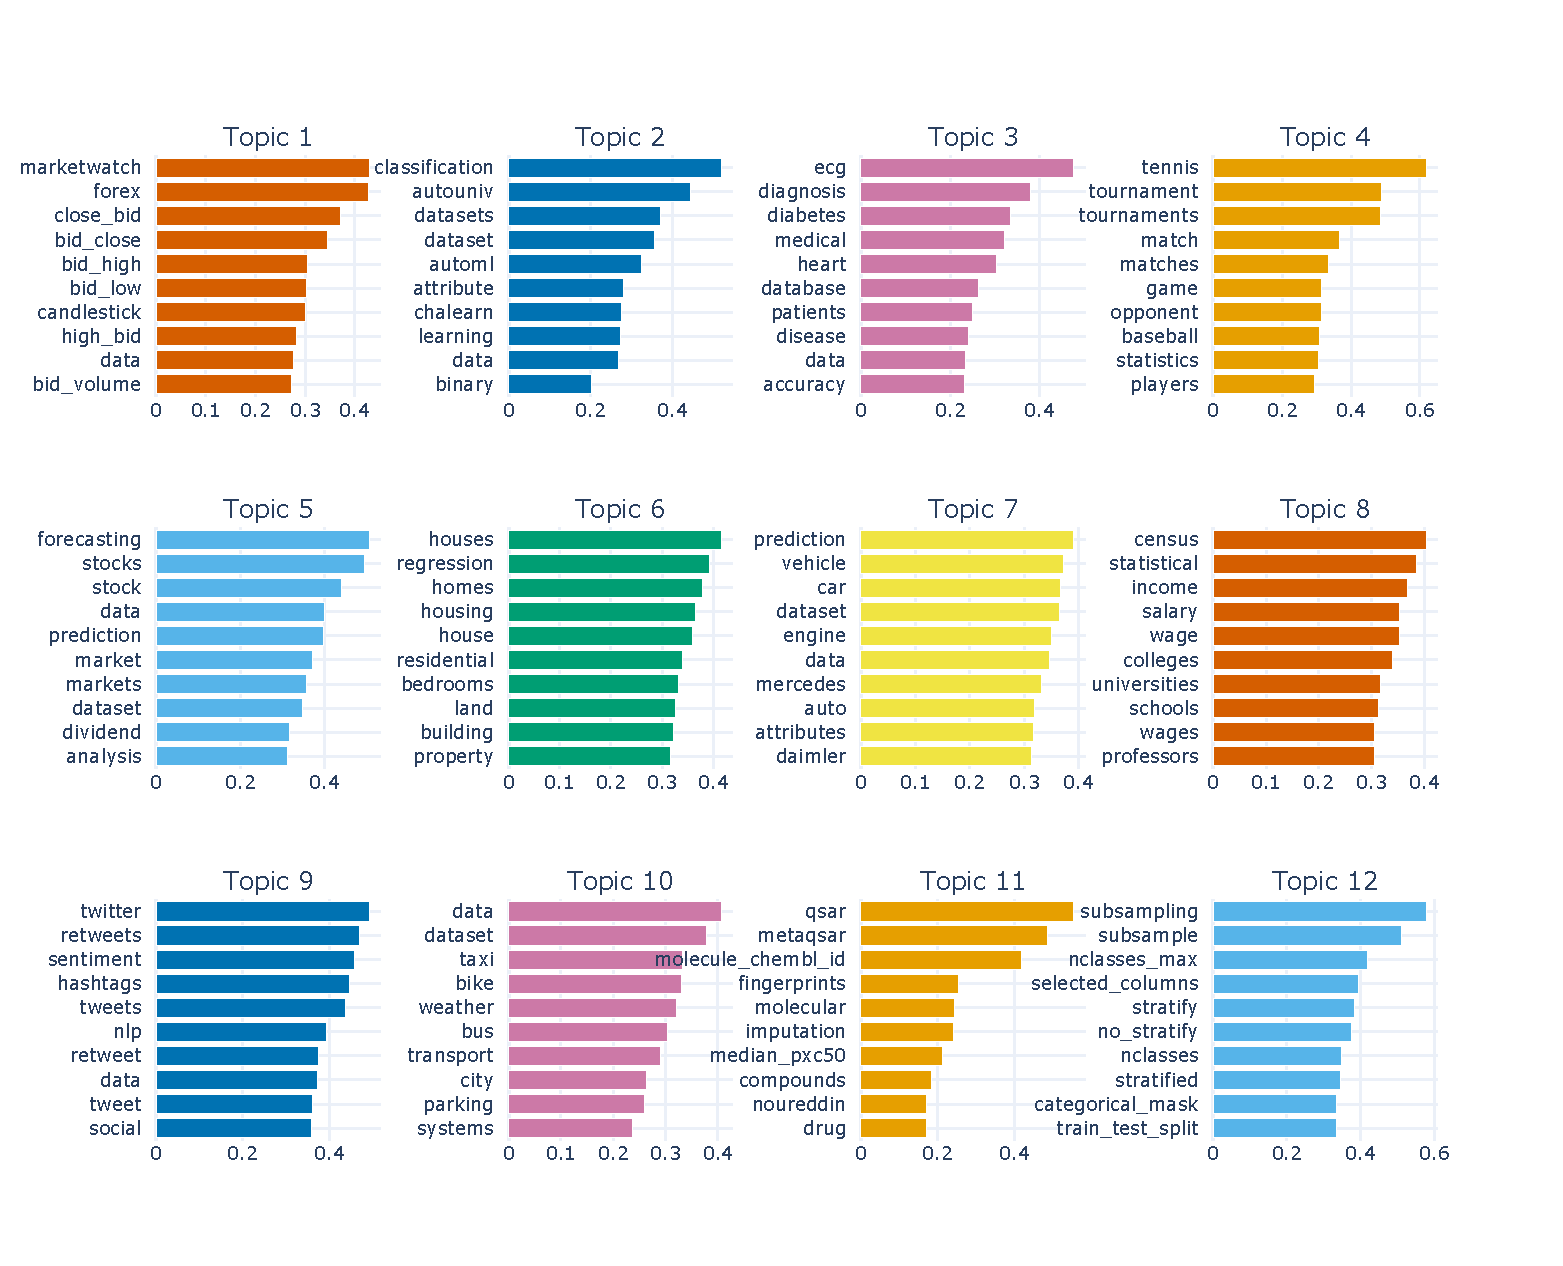
\includegraphics[width=\textwidth]{images/topics_barchart.pdf}
    \caption{Topic word scores}
    \label{fig:topics_barchart}
\end{figure}

However, it can be seen that certain topics contain terms that are not particularly useful. These terms often originate from documents that explain attribute values. For instance, \textit{Topic 11} and \textit{Topic 12} feature terms like \textit{median\_pxc50}, \textit{stratify}, \textit{no\_stratify}, and \textit{train\_test\_split}.

Additionally, many topics contain terms such as \textit{data}, \textit{dataset} and other similar terms that are not particularly descriptive.

Further experimentation with the model is necessary to address these cases.

% \todo[inline]{

% % - Discuss application of ChatGPT to classify topics by Taniya as a preliminary proof of concept?

% - Show my initial BERTopic application on the datasets which shows potential but also some of the challenges that will be faced - lack of descriptions of some datasets, arcane symbols and textual artifacts.


% }

%%------------------------------------------------------------------------------
\section{Other Information}
\label{sec:other}
%%------------------------------------------------------------------------------
\subsection{Data management}
% {
% \color{red}
% Responsible data management is part of good research. To promote effective and efficient data management, data sharing and data reuse, we expect researchers to carefully manage data. Research data are the evidence that underpin the answer to research questions, and can be used to validate findings. Data can be quantitative information or qualitative statements collected by researchers in the course of their work by experimentation, observation, modeling, interview or other methods, or information derived from existing evidence. 

% We understand software as included in the definition of research data. Algorithms, scripts and code developed by researchers in the course of their work may be necessary to access and interpret data. In such cases, the data management plan will be expected to address how information about such items will be made available.

% Research results should be stored in such a way that they can be retrieved and reproduced and/or reused in the long term, also by researchers in disciplines and organisations other than those in which the research took place. The operating principle is that all stored data are, in principle, freely accessible and that access is only limited if needed for reasons such as privacy, public security, ethical restrictions, property rights and commercial interests. Any tools or software (algorithms, scripts and code developed by researchers in the course of their work) necessary to access and interpret data should be made available alongside the data.

% \begin{enumerate}
% \item Will this project involve re-using existing research data?
% \begin{itemize}
% \item Yes: Are there any constraints on its re-use?
% \item No: Have you considered re-using existing data but discarded the possibility? Why?
% \end{itemize}

% \item Will data be collected or generated that are suitable for reuse? 
% \begin{itemize}
% \item Yes: Please answer question 3.
% \item No: Please explain why the research will not result in reusable data or in data that cannot be stored or data that for other reasons are not relevant for reuse. 
% \end{itemize}

% \item After the project has been completed, how will the data be stored for the long-term and made available for the use by third parties? Are there possible restrictions to data sharing or embargo reasons? Please state these here.
% \end{enumerate}
% }

This project will leverage existing datasets from the OpenML platform, utilizing its status as an open-source library with datasets that are freely and publicly accessible. Additionally, datasets from other open-source repositories, such as the Wolfram Data Repository \cite{noauthor_wolfram_nodate} or Huggingface \cite{noauthor_hugging_2024}, may also be employed.

The project will involve the collection and generation of data suitable for reuse. This data is not anticipated to include sensitive information, thus obviating the need for specialized treatment or storage.

Data produced by this project will be made publicly accessible via an open-source repository on a version control platform like GitHub \cite{noauthor_github_nodate}.

Regarding the data to be generated, it will contain a pipeline, including the initialization of data fetching (documents), data cleaning for the topic models, the implementation of the proposed topic model along with benchmark models, and the final output, which consists of a set of topic labels pertaining to the documents. Additionally, benchmarks will be generated based on the evaluation metrics.

\Cref{fig:data_pipeline} shows a flowchart of the pipeline, which contains the following sequential steps:

\begin{enumerate}

    \item \textbf{Data Fetching}: This is the first stage where dataset descriptions are downloaded from OpenML (or other sources).

    \item \textbf{Data Cleaning}: After fetching the data, the next step involves cleaning it. This includes removing noise, correcting errors, and standardizing the format to prepare it for analysis. Data cleaning ensures that the input to the topic model is of high quality, which is crucial for the success of the subsequent modeling steps.

          the next step involves purging inadequate data points, such as excessively short descriptions and duplicates. Stop words are removed for models that require it (LDA). Additionally, the process includes stemming and lemmatization to normalize words to their base forms.

    \item \textbf{Topic Model}: In this step, the proposed topic model is applied to the cleaned data. The topic model is an algorithm that discovers the underlying thematic structure in the collection of documents. In this case, it will be BERTopic.

    \item \textbf{Benchmark Models}: Concurrently with the proposed topic model, benchmark models are run. These models represent established or baseline approaches to topic modeling against which the performance of the proposed topic model is compared. This will involve baseline models such as LDA, NMF and Top2Vec.

    \item \textbf{Topic Labels}: The output from both the topic model and the benchmark models are sets of topics, represented by a cluster of words that are characteristic of a particular topic.

    \item \textbf{Evaluation}: Finally, the performances of the proposed topic model and benchmark models are evaluated. This can include comparing the topic coherence and diversity, as well as the relevance and interpretability of the topics generated. Evaluation metrics may also include quantitative measures such as perplexity, or qualitative assessments through human judgement.

\end{enumerate}

\begin{figure}[h] % adjust placement if needed
    \centering
    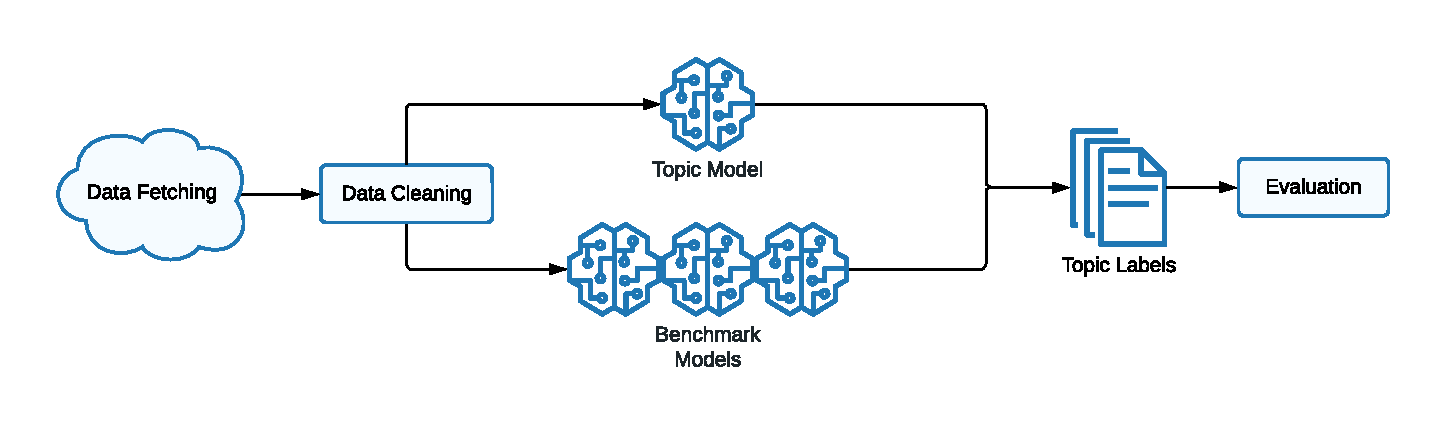
\includegraphics[width=\textwidth]{images/data_pipeline.pdf}
    \caption{Data pipeline}
    \label{fig:data_pipeline}
\end{figure}

% \todo[inline]{

% - Make data to be generated more detailed. Maybe include a figure of the pipeline.

% - Research and list evaluation metrics. List them in literature analysis part and reference them here.}

%%------------------------------------------------------------------------------
\subsection{Motivation for choice of research group / supervisor / company}
% {
% \color{red}
% This subsection can be used to explain why you have chosen this project with respect to supervisor, group and company. It is used to explain your view on the alignment of topic and the project team. 

% Note that the importance of each section and subsection and their respective content and size may vary from proposal to proposal. So you are expected to balance the content and length of each part accordingly. Typically Section~\ref{sec:other} is considerably smaller than the other sections. Often Sections~\ref{sec:goals}, \ref{sec:approach}, and~\ref{sec:evidence} are the largest sections.
% }

In the course of my Master's program, I enrolled in a course titled "Machine Learning Engineering." The course was led by Professor Joaquin Vanschoren, who participates in the Data Mining cluster at the TU/e. Furthermore, I followed several other courses related to machine learning, including "Research Topics in Data Mining," "Machine Learning for Industry," "Data Modeling and Databases," and "Deep Learning." These courses significantly improved my understanding and heightened my interest in the domain of machine learning. By focusing on topic modeling in my Master's thesis, I intend to continue broadening my knowledge and expertise in the field.

Additionally, the open-source status of OpenML played a role in attracting my interest. The prospect of contributing to an open-source project is appealing, since it is beneficial for the developer, practitioner, and research communities. This form of contribution furthers the knowledge in the field and makes it accessible to all.

\bibliographystyle{unsrtnat}
\bibliography{bibliography,references}

\appendix
\section{Appendix}
 {
  \color{red}

  You may provide any type of material as appendix to your project proposal. Typical appendices include additional details about the methodology, further pilot studies for illustration and demonstration of feasibility, images and results that were created, pointers to code (or pseudo-code itself), pointers to data, etc. There is no limit in the length of the appendices. For example, this appendix contain Table~\ref{table:somethinginside}, which has information that are not relevant but shows how to use a table here.

  \begin{table}[ht]
      \caption{Some results of something. It is recommend not to try to understand it.\label{table:somethinginside}}
      \begin{center}
          \begin{tabular}{cccc|cc|cc}
                      &                &           &       & \multicolumn{2}{c|}{Median} & \multicolumn{2}{c}{Maximum}                       \\
              Problem & Description    & Max Value & Nodes & Memory                      & Time(s)                     & Memory    & Time(s) \\
              \hline
              MINAP   & naive Bayes w/ & $10^{6}$  & 50    & $59$                        & $0.06$                      & $84$      & $0.08$  \\
                      & random params  &           & 100   & $125$                       & $0.198$                     & $200$     & $0.285$ \\
                      &                &           & 200   & $396$                       & $1.328$                     & $1238$    & $1.893$ \\
                      &                &           & 300   & $1103$                      & $2.793$                     & $20863$   & $9.893$ \\
              MAP     & naive Bayes w/ & $10^{6}$  & 50    & $5$                         & $0.01$                      & $7$       & $0.015$ \\
                      & random params  &           & 100   & $5$                         & $0.017$                     & $6$       & $0.023$ \\
                      &                &           & 200   & $5$                         & $0.04$                      & $7$       & $0.047$ \\
                      &                &           & 300   & $5$                         & $0.043$                     & $7$       & $0.049$ \\
              MINAP   & partition      & $10^{4}$  & 10    & $512$                       & $0.034$                     & $512$     & $0.039$ \\
                      & problem        &           & 20    & $91857$                     & $11.553$                    & $100842$  & $17.42$ \\
                      &                &           & 30    & $236979$                    & $77.09$                     & $264638$  & $82.81$ \\
                      &                & $10^{5}$  & 10    & $512$                       & $0.036$                     & $512$     & $0.045$ \\
                      &                &           & 20    & $347065$                    & $27.599$                    & $372670$  & $31.10$ \\
                      &                &           & 30    & $2046264$                   & $532.318$                   & $2237859$ & $586.4$ \\
                      &                & $10^{6}$  & 10    & $512$                       & $0.035$                     & $512$     & $0.038$ \\
                      &                &           & 20    & $501347$                    & $34.672$                    & $510413$  & $38.13$ \\
                      &                &           & 30    & $>10$Mln                    & $>600$                      & $>10$Mln  & $>600$  \\
              MINAP   & random struct. & $10^{6}$  & 50    & $57$                        & $0.046$                     & $101$     & $0.073$ \\
                      & and parameters &           & 100   & $143$                       & $0.21$                      & $197$     & $0.326$ \\
                      &                &           & 200   & $417$                       & $1.288$                     & $713$     & $1.761$ \\
                      &                &           & 300   & $1129$                      & $2.509$                     & $10403$   & $14.53$ \\
              MAP     & random struct. & $10^{6}$  & 50    & $5$                         & $0.009$                     & $7$       & $0.014$ \\
                      & and parameters &           & 100   & $5$                         & $0.018$                     & $6$       & $0.023$ \\
                      &                &           & 200   & $5$                         & $0.042$                     & $7$       & $0.047$ \\
                      &                &           & 300   & $6$                         & $0.049$                     & $7$       & $0.061$ \\
              \hline
          \end{tabular}
      \end{center}
  \end{table}

  \lipsum[1-4]
 }
\end{document}

